\documentclass[twoside]{book}

% Packages required by doxygen
\usepackage{fixltx2e}
\usepackage{calc}
\usepackage{doxygen}
\usepackage[export]{adjustbox} % also loads graphicx
\usepackage{graphicx}
\usepackage[utf8]{inputenc}
\usepackage{makeidx}
\usepackage{multicol}
\usepackage{multirow}
\PassOptionsToPackage{warn}{textcomp}
\usepackage{textcomp}
\usepackage[nointegrals]{wasysym}
\usepackage[table]{xcolor}

% Font selection
\usepackage[T1]{fontenc}
\usepackage[scaled=.90]{helvet}
\usepackage{courier}
\usepackage{amssymb}
\usepackage{sectsty}
\renewcommand{\familydefault}{\sfdefault}
\allsectionsfont{%
  \fontseries{bc}\selectfont%
  \color{darkgray}%
}
\renewcommand{\DoxyLabelFont}{%
  \fontseries{bc}\selectfont%
  \color{darkgray}%
}
\newcommand{\+}{\discretionary{\mbox{\scriptsize$\hookleftarrow$}}{}{}}

% Page & text layout
\usepackage{geometry}
\geometry{%
  a4paper,%
  top=2.5cm,%
  bottom=2.5cm,%
  left=2.5cm,%
  right=2.5cm%
}
\tolerance=750
\hfuzz=15pt
\hbadness=750
\setlength{\emergencystretch}{15pt}
\setlength{\parindent}{0cm}
\setlength{\parskip}{3ex plus 2ex minus 2ex}
\makeatletter
\renewcommand{\paragraph}{%
  \@startsection{paragraph}{4}{0ex}{-1.0ex}{1.0ex}{%
    \normalfont\normalsize\bfseries\SS@parafont%
  }%
}
\renewcommand{\subparagraph}{%
  \@startsection{subparagraph}{5}{0ex}{-1.0ex}{1.0ex}{%
    \normalfont\normalsize\bfseries\SS@subparafont%
  }%
}
\makeatother

% Headers & footers
\usepackage{fancyhdr}
\pagestyle{fancyplain}
\fancyhead[LE]{\fancyplain{}{\bfseries\thepage}}
\fancyhead[CE]{\fancyplain{}{}}
\fancyhead[RE]{\fancyplain{}{\bfseries\leftmark}}
\fancyhead[LO]{\fancyplain{}{\bfseries\rightmark}}
\fancyhead[CO]{\fancyplain{}{}}
\fancyhead[RO]{\fancyplain{}{\bfseries\thepage}}
\fancyfoot[LE]{\fancyplain{}{}}
\fancyfoot[CE]{\fancyplain{}{}}
\fancyfoot[RE]{\fancyplain{}{\bfseries\scriptsize Generated by Doxygen }}
\fancyfoot[LO]{\fancyplain{}{\bfseries\scriptsize Generated by Doxygen }}
\fancyfoot[CO]{\fancyplain{}{}}
\fancyfoot[RO]{\fancyplain{}{}}
\renewcommand{\footrulewidth}{0.4pt}
\renewcommand{\chaptermark}[1]{%
  \markboth{#1}{}%
}
\renewcommand{\sectionmark}[1]{%
  \markright{\thesection\ #1}%
}

% Indices & bibliography
\usepackage{natbib}
\usepackage[titles]{tocloft}
\setcounter{tocdepth}{3}
\setcounter{secnumdepth}{5}
\makeindex

% Hyperlinks (required, but should be loaded last)
\usepackage{ifpdf}
\ifpdf
  \usepackage[pdftex,pagebackref=true]{hyperref}
\else
  \usepackage[ps2pdf,pagebackref=true]{hyperref}
\fi
\hypersetup{%
  colorlinks=true,%
  linkcolor=blue,%
  citecolor=blue,%
  unicode%
}

% Custom commands
\newcommand{\clearemptydoublepage}{%
  \newpage{\pagestyle{empty}\cleardoublepage}%
}

\usepackage{caption}
\captionsetup{labelsep=space,justification=centering,font={bf},singlelinecheck=off,skip=4pt,position=top}

%===== C O N T E N T S =====

\begin{document}

% Titlepage & ToC
\hypersetup{pageanchor=false,
             bookmarksnumbered=true,
             pdfencoding=unicode
            }
\pagenumbering{alph}
\begin{titlepage}
\vspace*{7cm}
\begin{center}%
{\Large S\+F\+ML E\+N\+G\+I\+NE }\\
\vspace*{1cm}
{\large Generated by Doxygen 1.8.13}\\
\end{center}
\end{titlepage}
\clearemptydoublepage
\pagenumbering{roman}
\tableofcontents
\clearemptydoublepage
\pagenumbering{arabic}
\hypersetup{pageanchor=true}

%--- Begin generated contents ---
\chapter{Namespace Index}
\input{namespaces}
\chapter{Hierarchical Index}
\section{Class Hierarchy}
This inheritance list is sorted roughly, but not completely, alphabetically\+:\begin{DoxyCompactList}
\item \contentsline{section}{Map\+Layer\+:\+:Animation\+State}{\pageref{structMapLayer_1_1AnimationState}}{}
\item \contentsline{section}{b0x\+\_\+2d\+\_\+\+S\+H\+A\+P\+ES}{\pageref{structb0x__2d__SHAPES}}{}
\item \contentsline{section}{Character}{\pageref{structCharacter}}{}
\item Drawable\begin{DoxyCompactList}
\item \contentsline{section}{Map\+Layer}{\pageref{classMapLayer}}{}
\item \contentsline{section}{Map\+Layer\+:\+:Chunk}{\pageref{classMapLayer_1_1Chunk}}{}
\item \contentsline{section}{Map\+Layer\+:\+:Chunk\+:\+:Chunk\+Array}{\pageref{classMapLayer_1_1Chunk_1_1ChunkArray}}{}
\end{DoxyCompactList}
\item \contentsline{section}{Entity\+Manager}{\pageref{classEntityManager}}{}
\item \contentsline{section}{Game}{\pageref{classGame}}{}
\item \contentsline{section}{game\+\_\+text}{\pageref{classgame__text}}{}
\item \contentsline{section}{Game\+Data}{\pageref{structGameData}}{}
\item \contentsline{section}{Line}{\pageref{classLine}}{}
\item \contentsline{section}{Loading\+Game\+Objects}{\pageref{classLoadingGameObjects}}{}
\item \contentsline{section}{map}{\pageref{classmap}}{}
\item \contentsline{section}{Orthographic\+\_\+camera}{\pageref{classOrthographic__camera}}{}
\item \contentsline{section}{Resource\+Manager}{\pageref{classResourceManager}}{}
\item \contentsline{section}{Shader}{\pageref{classShader}}{}
\item \contentsline{section}{sprite}{\pageref{classsprite}}{}
\item \contentsline{section}{Sprite\+Renderer}{\pageref{classSpriteRenderer}}{}
\item \contentsline{section}{State}{\pageref{classState}}{}
\begin{DoxyCompactList}
\item \contentsline{section}{Game\+Over\+State}{\pageref{classGameOverState}}{}
\item \contentsline{section}{Game\+Play\+State}{\pageref{classGamePlayState}}{}
\item \contentsline{section}{Main\+Menu\+State}{\pageref{classMainMenuState}}{}
\item \contentsline{section}{Splash\+State}{\pageref{classSplashState}}{}
\end{DoxyCompactList}
\item \contentsline{section}{State\+Machine}{\pageref{classStateMachine}}{}
\item \contentsline{section}{stbi\+\_\+io\+\_\+callbacks}{\pageref{structstbi__io__callbacks}}{}
\item \contentsline{section}{Text\+Renderer}{\pageref{classTextRenderer}}{}
\item \contentsline{section}{Texture2D}{\pageref{classTexture2D}}{}
\begin{DoxyCompactList}
\item \contentsline{section}{Entity}{\pageref{classEntity}}{}
\end{DoxyCompactList}
\item Transformable\begin{DoxyCompactList}
\item \contentsline{section}{Map\+Layer\+:\+:Chunk}{\pageref{classMapLayer_1_1Chunk}}{}
\end{DoxyCompactList}
\end{DoxyCompactList}

\chapter{Class Index}
\section{Class List}
Here are the classes, structs, unions and interfaces with brief descriptions\+:\begin{DoxyCompactList}
\item\contentsline{section}{\hyperlink{structMapLayer_1_1AnimationState}{Map\+Layer\+::\+Animation\+State} }{\pageref{structMapLayer_1_1AnimationState}}{}
\item\contentsline{section}{\hyperlink{classSekander_1_1AssetManager}{Sekander\+::\+Asset\+Manager} }{\pageref{classSekander_1_1AssetManager}}{}
\item\contentsline{section}{\hyperlink{structSekander_1_1b0x__2d__SHAPES}{Sekander\+::b0x\+\_\+2d\+\_\+\+S\+H\+A\+P\+ES} }{\pageref{structSekander_1_1b0x__2d__SHAPES}}{}
\item\contentsline{section}{\hyperlink{classSekander_1_1Bullet}{Sekander\+::\+Bullet} }{\pageref{classSekander_1_1Bullet}}{}
\item\contentsline{section}{\hyperlink{classSekander_1_1Button}{Sekander\+::\+Button} }{\pageref{classSekander_1_1Button}}{}
\item\contentsline{section}{\hyperlink{classMapLayer_1_1Chunk}{Map\+Layer\+::\+Chunk} }{\pageref{classMapLayer_1_1Chunk}}{}
\item\contentsline{section}{\hyperlink{classMapLayer_1_1Chunk_1_1ChunkArray}{Map\+Layer\+::\+Chunk\+::\+Chunk\+Array} }{\pageref{classMapLayer_1_1Chunk_1_1ChunkArray}}{}
\item\contentsline{section}{\hyperlink{classSekander_1_1Enemy}{Sekander\+::\+Enemy} }{\pageref{classSekander_1_1Enemy}}{}
\item\contentsline{section}{\hyperlink{classSekander_1_1Entity}{Sekander\+::\+Entity} }{\pageref{classSekander_1_1Entity}}{}
\item\contentsline{section}{\hyperlink{classSekander_1_1EntityManager}{Sekander\+::\+Entity\+Manager} }{\pageref{classSekander_1_1EntityManager}}{}
\item\contentsline{section}{\hyperlink{classSekander_1_1Game}{Sekander\+::\+Game} }{\pageref{classSekander_1_1Game}}{}
\item\contentsline{section}{\hyperlink{structSekander_1_1GameData}{Sekander\+::\+Game\+Data} }{\pageref{structSekander_1_1GameData}}{}
\item\contentsline{section}{\hyperlink{classSekander_1_1GameOverState}{Sekander\+::\+Game\+Over\+State} }{\pageref{classSekander_1_1GameOverState}}{}
\item\contentsline{section}{\hyperlink{classSekander_1_1GameState}{Sekander\+::\+Game\+State} }{\pageref{classSekander_1_1GameState}}{}
\item\contentsline{section}{\hyperlink{classSekander_1_1GameWorld}{Sekander\+::\+Game\+World} }{\pageref{classSekander_1_1GameWorld}}{}
\item\contentsline{section}{\hyperlink{classSekander_1_1Gun}{Sekander\+::\+Gun} }{\pageref{classSekander_1_1Gun}}{}
\item\contentsline{section}{\hyperlink{classSekander_1_1HUD}{Sekander\+::\+H\+UD} }{\pageref{classSekander_1_1HUD}}{}
\item\contentsline{section}{\hyperlink{classSekander_1_1InputManager}{Sekander\+::\+Input\+Manager} }{\pageref{classSekander_1_1InputManager}}{}
\item\contentsline{section}{\hyperlink{classSekander_1_1LoadingGameObjects}{Sekander\+::\+Loading\+Game\+Objects} }{\pageref{classSekander_1_1LoadingGameObjects}}{}
\item\contentsline{section}{\hyperlink{classSekander_1_1Main__Player}{Sekander\+::\+Main\+\_\+\+Player} }{\pageref{classSekander_1_1Main__Player}}{}
\item\contentsline{section}{\hyperlink{classSekander_1_1MainMenuState}{Sekander\+::\+Main\+Menu\+State} }{\pageref{classSekander_1_1MainMenuState}}{}
\item\contentsline{section}{\hyperlink{classMapLayer}{Map\+Layer} }{\pageref{classMapLayer}}{}
\item\contentsline{section}{\hyperlink{classSekander_1_1SplashState}{Sekander\+::\+Splash\+State} }{\pageref{classSekander_1_1SplashState}}{}
\item\contentsline{section}{\hyperlink{classSekander_1_1State}{Sekander\+::\+State} }{\pageref{classSekander_1_1State}}{}
\item\contentsline{section}{\hyperlink{classSekander_1_1StateMachine}{Sekander\+::\+State\+Machine} }{\pageref{classSekander_1_1StateMachine}}{}
\item\contentsline{section}{\hyperlink{classTileMap}{Tile\+Map} }{\pageref{classTileMap}}{}
\end{DoxyCompactList}

\chapter{File Index}
\section{File List}
Here is a list of all files with brief descriptions\+:\begin{DoxyCompactList}
\item\contentsline{section}{/mnt/hdd/\+C0de/\+Engines/\+S\+F\+M\+L/\+S\+F\+M\+L\+\_\+\+Engine/include/\hyperlink{AssetManager_8hpp}{Asset\+Manager.\+hpp} }{\pageref{AssetManager_8hpp}}{}
\item\contentsline{section}{/mnt/hdd/\+C0de/\+Engines/\+S\+F\+M\+L/\+S\+F\+M\+L\+\_\+\+Engine/include/\hyperlink{Bullet_8hpp}{Bullet.\+hpp} }{\pageref{Bullet_8hpp}}{}
\item\contentsline{section}{/mnt/hdd/\+C0de/\+Engines/\+S\+F\+M\+L/\+S\+F\+M\+L\+\_\+\+Engine/include/\hyperlink{Button_8hpp}{Button.\+hpp} }{\pageref{Button_8hpp}}{}
\item\contentsline{section}{/mnt/hdd/\+C0de/\+Engines/\+S\+F\+M\+L/\+S\+F\+M\+L\+\_\+\+Engine/include/\hyperlink{DEFINITIONS_8hpp}{D\+E\+F\+I\+N\+I\+T\+I\+O\+N\+S.\+hpp} }{\pageref{DEFINITIONS_8hpp}}{}
\item\contentsline{section}{/mnt/hdd/\+C0de/\+Engines/\+S\+F\+M\+L/\+S\+F\+M\+L\+\_\+\+Engine/include/\hyperlink{Enemy_8hpp}{Enemy.\+hpp} }{\pageref{Enemy_8hpp}}{}
\item\contentsline{section}{/mnt/hdd/\+C0de/\+Engines/\+S\+F\+M\+L/\+S\+F\+M\+L\+\_\+\+Engine/include/\hyperlink{entity_8h}{entity.\+h} }{\pageref{entity_8h}}{}
\item\contentsline{section}{/mnt/hdd/\+C0de/\+Engines/\+S\+F\+M\+L/\+S\+F\+M\+L\+\_\+\+Engine/include/\hyperlink{entity__manager_8h}{entity\+\_\+manager.\+h} }{\pageref{entity__manager_8h}}{}
\item\contentsline{section}{/mnt/hdd/\+C0de/\+Engines/\+S\+F\+M\+L/\+S\+F\+M\+L\+\_\+\+Engine/include/\hyperlink{Game_8hpp}{Game.\+hpp} }{\pageref{Game_8hpp}}{}
\item\contentsline{section}{/mnt/hdd/\+C0de/\+Engines/\+S\+F\+M\+L/\+S\+F\+M\+L\+\_\+\+Engine/include/\hyperlink{GameOverState_8hpp}{Game\+Over\+State.\+hpp} }{\pageref{GameOverState_8hpp}}{}
\item\contentsline{section}{/mnt/hdd/\+C0de/\+Engines/\+S\+F\+M\+L/\+S\+F\+M\+L\+\_\+\+Engine/include/\hyperlink{GameState_8hpp}{Game\+State.\+hpp} }{\pageref{GameState_8hpp}}{}
\item\contentsline{section}{/mnt/hdd/\+C0de/\+Engines/\+S\+F\+M\+L/\+S\+F\+M\+L\+\_\+\+Engine/include/\hyperlink{GameWorld_8hpp}{Game\+World.\+hpp} }{\pageref{GameWorld_8hpp}}{}
\item\contentsline{section}{/mnt/hdd/\+C0de/\+Engines/\+S\+F\+M\+L/\+S\+F\+M\+L\+\_\+\+Engine/include/\hyperlink{Gun_8hpp}{Gun.\+hpp} }{\pageref{Gun_8hpp}}{}
\item\contentsline{section}{/mnt/hdd/\+C0de/\+Engines/\+S\+F\+M\+L/\+S\+F\+M\+L\+\_\+\+Engine/include/\hyperlink{HUD_8hpp}{H\+U\+D.\+hpp} }{\pageref{HUD_8hpp}}{}
\item\contentsline{section}{/mnt/hdd/\+C0de/\+Engines/\+S\+F\+M\+L/\+S\+F\+M\+L\+\_\+\+Engine/include/\hyperlink{InputManager_8hpp}{Input\+Manager.\+hpp} }{\pageref{InputManager_8hpp}}{}
\item\contentsline{section}{/mnt/hdd/\+C0de/\+Engines/\+S\+F\+M\+L/\+S\+F\+M\+L\+\_\+\+Engine/include/\hyperlink{LoadingGameObjects_8hpp}{Loading\+Game\+Objects.\+hpp} }{\pageref{LoadingGameObjects_8hpp}}{}
\item\contentsline{section}{/mnt/hdd/\+C0de/\+Engines/\+S\+F\+M\+L/\+S\+F\+M\+L\+\_\+\+Engine/include/\hyperlink{Main__Player_8hpp}{Main\+\_\+\+Player.\+hpp} }{\pageref{Main__Player_8hpp}}{}
\item\contentsline{section}{/mnt/hdd/\+C0de/\+Engines/\+S\+F\+M\+L/\+S\+F\+M\+L\+\_\+\+Engine/include/\hyperlink{MainMenuState_8hpp}{Main\+Menu\+State.\+hpp} }{\pageref{MainMenuState_8hpp}}{}
\item\contentsline{section}{/mnt/hdd/\+C0de/\+Engines/\+S\+F\+M\+L/\+S\+F\+M\+L\+\_\+\+Engine/include/\hyperlink{SFMLOrthogonalLayer_8hpp}{S\+F\+M\+L\+Orthogonal\+Layer.\+hpp} }{\pageref{SFMLOrthogonalLayer_8hpp}}{}
\item\contentsline{section}{/mnt/hdd/\+C0de/\+Engines/\+S\+F\+M\+L/\+S\+F\+M\+L\+\_\+\+Engine/include/\hyperlink{SplashState_8hpp}{Splash\+State.\+hpp} }{\pageref{SplashState_8hpp}}{}
\item\contentsline{section}{/mnt/hdd/\+C0de/\+Engines/\+S\+F\+M\+L/\+S\+F\+M\+L\+\_\+\+Engine/include/\hyperlink{State_8hpp}{State.\+hpp} }{\pageref{State_8hpp}}{}
\item\contentsline{section}{/mnt/hdd/\+C0de/\+Engines/\+S\+F\+M\+L/\+S\+F\+M\+L\+\_\+\+Engine/include/\hyperlink{StateMachine_8hpp}{State\+Machine.\+hpp} }{\pageref{StateMachine_8hpp}}{}
\item\contentsline{section}{/mnt/hdd/\+C0de/\+Engines/\+S\+F\+M\+L/\+S\+F\+M\+L\+\_\+\+Engine/include/\hyperlink{TileMap_8hpp}{Tile\+Map.\+hpp} }{\pageref{TileMap_8hpp}}{}
\item\contentsline{section}{/mnt/hdd/\+C0de/\+Engines/\+S\+F\+M\+L/\+S\+F\+M\+L\+\_\+\+Engine/src/\hyperlink{AssetManager_8cpp}{Asset\+Manager.\+cpp} }{\pageref{AssetManager_8cpp}}{}
\item\contentsline{section}{/mnt/hdd/\+C0de/\+Engines/\+S\+F\+M\+L/\+S\+F\+M\+L\+\_\+\+Engine/src/\hyperlink{Bullet_8cpp}{Bullet.\+cpp} }{\pageref{Bullet_8cpp}}{}
\item\contentsline{section}{/mnt/hdd/\+C0de/\+Engines/\+S\+F\+M\+L/\+S\+F\+M\+L\+\_\+\+Engine/src/\hyperlink{Enemy_8cpp}{Enemy.\+cpp} }{\pageref{Enemy_8cpp}}{}
\item\contentsline{section}{/mnt/hdd/\+C0de/\+Engines/\+S\+F\+M\+L/\+S\+F\+M\+L\+\_\+\+Engine/src/\hyperlink{entity_8cpp}{entity.\+cpp} }{\pageref{entity_8cpp}}{}
\item\contentsline{section}{/mnt/hdd/\+C0de/\+Engines/\+S\+F\+M\+L/\+S\+F\+M\+L\+\_\+\+Engine/src/\hyperlink{entity__manager_8cpp}{entity\+\_\+manager.\+cpp} }{\pageref{entity__manager_8cpp}}{}
\item\contentsline{section}{/mnt/hdd/\+C0de/\+Engines/\+S\+F\+M\+L/\+S\+F\+M\+L\+\_\+\+Engine/src/\hyperlink{Game_8cpp}{Game.\+cpp} }{\pageref{Game_8cpp}}{}
\item\contentsline{section}{/mnt/hdd/\+C0de/\+Engines/\+S\+F\+M\+L/\+S\+F\+M\+L\+\_\+\+Engine/src/\hyperlink{GameOverState_8cpp}{Game\+Over\+State.\+cpp} }{\pageref{GameOverState_8cpp}}{}
\item\contentsline{section}{/mnt/hdd/\+C0de/\+Engines/\+S\+F\+M\+L/\+S\+F\+M\+L\+\_\+\+Engine/src/\hyperlink{GameState_8cpp}{Game\+State.\+cpp} }{\pageref{GameState_8cpp}}{}
\item\contentsline{section}{/mnt/hdd/\+C0de/\+Engines/\+S\+F\+M\+L/\+S\+F\+M\+L\+\_\+\+Engine/src/\hyperlink{GameWorld_8cpp}{Game\+World.\+cpp} }{\pageref{GameWorld_8cpp}}{}
\item\contentsline{section}{/mnt/hdd/\+C0de/\+Engines/\+S\+F\+M\+L/\+S\+F\+M\+L\+\_\+\+Engine/src/\hyperlink{Gun_8cpp}{Gun.\+cpp} }{\pageref{Gun_8cpp}}{}
\item\contentsline{section}{/mnt/hdd/\+C0de/\+Engines/\+S\+F\+M\+L/\+S\+F\+M\+L\+\_\+\+Engine/src/\hyperlink{HUD_8cpp}{H\+U\+D.\+cpp} }{\pageref{HUD_8cpp}}{}
\item\contentsline{section}{/mnt/hdd/\+C0de/\+Engines/\+S\+F\+M\+L/\+S\+F\+M\+L\+\_\+\+Engine/src/\hyperlink{InputManager_8cpp}{Input\+Manager.\+cpp} }{\pageref{InputManager_8cpp}}{}
\item\contentsline{section}{/mnt/hdd/\+C0de/\+Engines/\+S\+F\+M\+L/\+S\+F\+M\+L\+\_\+\+Engine/src/\hyperlink{LoadingGameObjects_8cpp}{Loading\+Game\+Objects.\+cpp} }{\pageref{LoadingGameObjects_8cpp}}{}
\item\contentsline{section}{/mnt/hdd/\+C0de/\+Engines/\+S\+F\+M\+L/\+S\+F\+M\+L\+\_\+\+Engine/src/\hyperlink{main_8cpp}{main.\+cpp} }{\pageref{main_8cpp}}{}
\item\contentsline{section}{/mnt/hdd/\+C0de/\+Engines/\+S\+F\+M\+L/\+S\+F\+M\+L\+\_\+\+Engine/src/\hyperlink{Main__Player_8cpp}{Main\+\_\+\+Player.\+cpp} }{\pageref{Main__Player_8cpp}}{}
\item\contentsline{section}{/mnt/hdd/\+C0de/\+Engines/\+S\+F\+M\+L/\+S\+F\+M\+L\+\_\+\+Engine/src/\hyperlink{MainMenuState_8cpp}{Main\+Menu\+State.\+cpp} }{\pageref{MainMenuState_8cpp}}{}
\item\contentsline{section}{/mnt/hdd/\+C0de/\+Engines/\+S\+F\+M\+L/\+S\+F\+M\+L\+\_\+\+Engine/src/\hyperlink{SplashState_8cpp}{Splash\+State.\+cpp} }{\pageref{SplashState_8cpp}}{}
\item\contentsline{section}{/mnt/hdd/\+C0de/\+Engines/\+S\+F\+M\+L/\+S\+F\+M\+L\+\_\+\+Engine/src/\hyperlink{StateMachine_8cpp}{State\+Machine.\+cpp} }{\pageref{StateMachine_8cpp}}{}
\end{DoxyCompactList}

\chapter{Namespace Documentation}
\hypertarget{namespaceSekander}{}\section{Sekander Namespace Reference}
\label{namespaceSekander}\index{Sekander@{Sekander}}
\subsection*{Classes}
\begin{DoxyCompactItemize}
\item 
class \hyperlink{classSekander_1_1AssetManager}{Asset\+Manager}
\item 
struct \hyperlink{structSekander_1_1b0x__2d__SHAPES}{b0x\+\_\+2d\+\_\+\+S\+H\+A\+P\+ES}
\item 
class \hyperlink{classSekander_1_1Bullet}{Bullet}
\item 
class \hyperlink{classSekander_1_1Button}{Button}
\item 
class \hyperlink{classSekander_1_1Enemy}{Enemy}
\item 
class \hyperlink{classSekander_1_1Entity}{Entity}
\item 
class \hyperlink{classSekander_1_1EntityManager}{Entity\+Manager}
\item 
class \hyperlink{classSekander_1_1Game}{Game}
\item 
struct \hyperlink{structSekander_1_1GameData}{Game\+Data}
\item 
class \hyperlink{classSekander_1_1GameOverState}{Game\+Over\+State}
\item 
class \hyperlink{classSekander_1_1GameState}{Game\+State}
\item 
class \hyperlink{classSekander_1_1GameWorld}{Game\+World}
\item 
class \hyperlink{classSekander_1_1Gun}{Gun}
\item 
class \hyperlink{classSekander_1_1HUD}{H\+UD}
\item 
class \hyperlink{classSekander_1_1InputManager}{Input\+Manager}
\item 
class \hyperlink{classSekander_1_1LoadingGameObjects}{Loading\+Game\+Objects}
\item 
class \hyperlink{classSekander_1_1Main__Player}{Main\+\_\+\+Player}
\item 
class \hyperlink{classSekander_1_1MainMenuState}{Main\+Menu\+State}
\item 
class \hyperlink{classSekander_1_1SplashState}{Splash\+State}
\item 
class \hyperlink{classSekander_1_1State}{State}
\item 
class \hyperlink{classSekander_1_1StateMachine}{State\+Machine}
\end{DoxyCompactItemize}
\subsection*{Typedefs}
\begin{DoxyCompactItemize}
\item 
typedef std\+::shared\+\_\+ptr$<$ \hyperlink{structSekander_1_1GameData}{Game\+Data} $>$ \hyperlink{namespaceSekander_a1d69b002ba2d23020901c28f0def5e16}{Game\+Data\+Ref}
\item 
typedef std\+::unique\+\_\+ptr$<$ \hyperlink{classSekander_1_1State}{State} $>$ \hyperlink{namespaceSekander_a8503cedf9c863e9f6986eb29f2296f1a}{State\+Ref}
\end{DoxyCompactItemize}
\subsection*{Enumerations}
\begin{DoxyCompactItemize}
\item 
enum \hyperlink{namespaceSekander_aed8eb219f4685b29738464e9f32c5d94}{shape\+\_\+options} \{ \hyperlink{namespaceSekander_aed8eb219f4685b29738464e9f32c5d94ae1827bea553b36ce0bbc7cddd6c57621}{Square} = 1, 
\hyperlink{namespaceSekander_aed8eb219f4685b29738464e9f32c5d94acafcba9574f3415e8e9f6f194a6cb869}{Circle} = 2
 \}
\end{DoxyCompactItemize}
\subsection*{Functions}
\begin{DoxyCompactItemize}
\item 
void \hyperlink{namespaceSekander_a9abc849b0e833c5c6f3a8b33bdd3f763}{callback\+Func} ()
\end{DoxyCompactItemize}


\subsection{Typedef Documentation}
\mbox{\Hypertarget{namespaceSekander_a1d69b002ba2d23020901c28f0def5e16}\label{namespaceSekander_a1d69b002ba2d23020901c28f0def5e16}} 
\index{Sekander@{Sekander}!Game\+Data\+Ref@{Game\+Data\+Ref}}
\index{Game\+Data\+Ref@{Game\+Data\+Ref}!Sekander@{Sekander}}
\subsubsection{\texorpdfstring{Game\+Data\+Ref}{GameDataRef}}
{\footnotesize\ttfamily typedef std\+::shared\+\_\+ptr$<$\hyperlink{structSekander_1_1GameData}{Game\+Data}$>$ \hyperlink{namespaceSekander_a1d69b002ba2d23020901c28f0def5e16}{Sekander\+::\+Game\+Data\+Ref}}

\mbox{\Hypertarget{namespaceSekander_a8503cedf9c863e9f6986eb29f2296f1a}\label{namespaceSekander_a8503cedf9c863e9f6986eb29f2296f1a}} 
\index{Sekander@{Sekander}!State\+Ref@{State\+Ref}}
\index{State\+Ref@{State\+Ref}!Sekander@{Sekander}}
\subsubsection{\texorpdfstring{State\+Ref}{StateRef}}
{\footnotesize\ttfamily typedef std\+::unique\+\_\+ptr$<$\hyperlink{classSekander_1_1State}{State}$>$ \hyperlink{namespaceSekander_a8503cedf9c863e9f6986eb29f2296f1a}{Sekander\+::\+State\+Ref}}



\subsection{Enumeration Type Documentation}
\mbox{\Hypertarget{namespaceSekander_aed8eb219f4685b29738464e9f32c5d94}\label{namespaceSekander_aed8eb219f4685b29738464e9f32c5d94}} 
\index{Sekander@{Sekander}!shape\+\_\+options@{shape\+\_\+options}}
\index{shape\+\_\+options@{shape\+\_\+options}!Sekander@{Sekander}}
\subsubsection{\texorpdfstring{shape\+\_\+options}{shape\_options}}
{\footnotesize\ttfamily enum \hyperlink{namespaceSekander_aed8eb219f4685b29738464e9f32c5d94}{Sekander\+::shape\+\_\+options}}

\begin{DoxyEnumFields}{Enumerator}
\raisebox{\heightof{T}}[0pt][0pt]{\index{Square@{Square}!Sekander@{Sekander}}\index{Sekander@{Sekander}!Square@{Square}}}\mbox{\Hypertarget{namespaceSekander_aed8eb219f4685b29738464e9f32c5d94ae1827bea553b36ce0bbc7cddd6c57621}\label{namespaceSekander_aed8eb219f4685b29738464e9f32c5d94ae1827bea553b36ce0bbc7cddd6c57621}} 
Square&\\
\hline

\raisebox{\heightof{T}}[0pt][0pt]{\index{Circle@{Circle}!Sekander@{Sekander}}\index{Sekander@{Sekander}!Circle@{Circle}}}\mbox{\Hypertarget{namespaceSekander_aed8eb219f4685b29738464e9f32c5d94acafcba9574f3415e8e9f6f194a6cb869}\label{namespaceSekander_aed8eb219f4685b29738464e9f32c5d94acafcba9574f3415e8e9f6f194a6cb869}} 
Circle&\\
\hline

\end{DoxyEnumFields}


\subsection{Function Documentation}
\mbox{\Hypertarget{namespaceSekander_a9abc849b0e833c5c6f3a8b33bdd3f763}\label{namespaceSekander_a9abc849b0e833c5c6f3a8b33bdd3f763}} 
\index{Sekander@{Sekander}!callback\+Func@{callback\+Func}}
\index{callback\+Func@{callback\+Func}!Sekander@{Sekander}}
\subsubsection{\texorpdfstring{callback\+Func()}{callbackFunc()}}
{\footnotesize\ttfamily void Sekander\+::callback\+Func (\begin{DoxyParamCaption}{ }\end{DoxyParamCaption})}


\chapter{Class Documentation}
\hypertarget{structMapLayer_1_1AnimationState}{}\section{Map\+Layer\+:\+:Animation\+State Struct Reference}
\label{structMapLayer_1_1AnimationState}\index{Map\+Layer\+::\+Animation\+State@{Map\+Layer\+::\+Animation\+State}}


Collaboration diagram for Map\+Layer\+:\+:Animation\+State\+:
\nopagebreak
\begin{figure}[H]
\begin{center}
\leavevmode
\includegraphics[width=212pt]{structMapLayer_1_1AnimationState__coll__graph}
\end{center}
\end{figure}
\subsection*{Public Attributes}
\begin{DoxyCompactItemize}
\item 
sf\+::\+Vector2u \hyperlink{structMapLayer_1_1AnimationState_ab37c9495a8dce1f661f1f4e46b77f17f}{tile\+Cords}
\item 
sf\+::\+Time \hyperlink{structMapLayer_1_1AnimationState_aa9d9ceefb1f56dac58bc7660a1ba7898}{start\+Time}
\item 
sf\+::\+Time \hyperlink{structMapLayer_1_1AnimationState_a836c7a2799636527b08eeeb1783069e8}{current\+Time}
\item 
tmx\+::\+Tileset\+::\+Tile \hyperlink{structMapLayer_1_1AnimationState_aabe80ae4711c86db562b3e7b5e3bb6d1}{anim\+Tile}
\item 
std\+::uint8\+\_\+t \hyperlink{structMapLayer_1_1AnimationState_aa880baa2bb7e1e2f02d37ce7a6c0dc8a}{flip\+Flags}
\end{DoxyCompactItemize}


\subsection{Member Data Documentation}
\mbox{\Hypertarget{structMapLayer_1_1AnimationState_aabe80ae4711c86db562b3e7b5e3bb6d1}\label{structMapLayer_1_1AnimationState_aabe80ae4711c86db562b3e7b5e3bb6d1}} 
\index{Map\+Layer\+::\+Animation\+State@{Map\+Layer\+::\+Animation\+State}!anim\+Tile@{anim\+Tile}}
\index{anim\+Tile@{anim\+Tile}!Map\+Layer\+::\+Animation\+State@{Map\+Layer\+::\+Animation\+State}}
\subsubsection{\texorpdfstring{anim\+Tile}{animTile}}
{\footnotesize\ttfamily tmx\+::\+Tileset\+::\+Tile Map\+Layer\+::\+Animation\+State\+::anim\+Tile}

\mbox{\Hypertarget{structMapLayer_1_1AnimationState_a836c7a2799636527b08eeeb1783069e8}\label{structMapLayer_1_1AnimationState_a836c7a2799636527b08eeeb1783069e8}} 
\index{Map\+Layer\+::\+Animation\+State@{Map\+Layer\+::\+Animation\+State}!current\+Time@{current\+Time}}
\index{current\+Time@{current\+Time}!Map\+Layer\+::\+Animation\+State@{Map\+Layer\+::\+Animation\+State}}
\subsubsection{\texorpdfstring{current\+Time}{currentTime}}
{\footnotesize\ttfamily sf\+::\+Time Map\+Layer\+::\+Animation\+State\+::current\+Time}

\mbox{\Hypertarget{structMapLayer_1_1AnimationState_aa880baa2bb7e1e2f02d37ce7a6c0dc8a}\label{structMapLayer_1_1AnimationState_aa880baa2bb7e1e2f02d37ce7a6c0dc8a}} 
\index{Map\+Layer\+::\+Animation\+State@{Map\+Layer\+::\+Animation\+State}!flip\+Flags@{flip\+Flags}}
\index{flip\+Flags@{flip\+Flags}!Map\+Layer\+::\+Animation\+State@{Map\+Layer\+::\+Animation\+State}}
\subsubsection{\texorpdfstring{flip\+Flags}{flipFlags}}
{\footnotesize\ttfamily std\+::uint8\+\_\+t Map\+Layer\+::\+Animation\+State\+::flip\+Flags}

\mbox{\Hypertarget{structMapLayer_1_1AnimationState_aa9d9ceefb1f56dac58bc7660a1ba7898}\label{structMapLayer_1_1AnimationState_aa9d9ceefb1f56dac58bc7660a1ba7898}} 
\index{Map\+Layer\+::\+Animation\+State@{Map\+Layer\+::\+Animation\+State}!start\+Time@{start\+Time}}
\index{start\+Time@{start\+Time}!Map\+Layer\+::\+Animation\+State@{Map\+Layer\+::\+Animation\+State}}
\subsubsection{\texorpdfstring{start\+Time}{startTime}}
{\footnotesize\ttfamily sf\+::\+Time Map\+Layer\+::\+Animation\+State\+::start\+Time}

\mbox{\Hypertarget{structMapLayer_1_1AnimationState_ab37c9495a8dce1f661f1f4e46b77f17f}\label{structMapLayer_1_1AnimationState_ab37c9495a8dce1f661f1f4e46b77f17f}} 
\index{Map\+Layer\+::\+Animation\+State@{Map\+Layer\+::\+Animation\+State}!tile\+Cords@{tile\+Cords}}
\index{tile\+Cords@{tile\+Cords}!Map\+Layer\+::\+Animation\+State@{Map\+Layer\+::\+Animation\+State}}
\subsubsection{\texorpdfstring{tile\+Cords}{tileCords}}
{\footnotesize\ttfamily sf\+::\+Vector2u Map\+Layer\+::\+Animation\+State\+::tile\+Cords}



The documentation for this struct was generated from the following file\+:\begin{DoxyCompactItemize}
\item 
/mnt/hdd/\+C0de/smart\+\_\+engine/include/\hyperlink{SFMLOrthogonalLayer_8hpp}{S\+F\+M\+L\+Orthogonal\+Layer.\+hpp}\end{DoxyCompactItemize}

\hypertarget{classSekander_1_1AssetManager}{}\section{Sekander\+:\+:Asset\+Manager Class Reference}
\label{classSekander_1_1AssetManager}\index{Sekander\+::\+Asset\+Manager@{Sekander\+::\+Asset\+Manager}}


{\ttfamily \#include $<$Asset\+Manager.\+hpp$>$}



Collaboration diagram for Sekander\+:\+:Asset\+Manager\+:
\nopagebreak
\begin{figure}[H]
\begin{center}
\leavevmode
\includegraphics[width=207pt]{classSekander_1_1AssetManager__coll__graph}
\end{center}
\end{figure}
\subsection*{Public Member Functions}
\begin{DoxyCompactItemize}
\item 
\hyperlink{classSekander_1_1AssetManager_a5d122bc31351cdf6a844d97351243b1b}{Asset\+Manager} ()
\item 
\hyperlink{classSekander_1_1AssetManager_a471be342805da815a3de41b72ed6a763}{$\sim$\+Asset\+Manager} ()
\item 
void \hyperlink{classSekander_1_1AssetManager_a49871c9808fc5e2988059c92fb181c67}{Load\+Texture} (std\+::string name, std\+::string file\+Name)
\item 
sf\+::\+Texture \& \hyperlink{classSekander_1_1AssetManager_a276ceaa15497655f3ecf24d1b74b5122}{Get\+Texture} (std\+::string name)
\item 
void \hyperlink{classSekander_1_1AssetManager_adec8c37238ad13c8756c13ed845150e3}{Load\+Font} (std\+::string name, std\+::string file\+Name)
\item 
sf\+::\+Font \& \hyperlink{classSekander_1_1AssetManager_a745b3164696e8a92fb479119d11ac034}{Get\+Font} (std\+::string name)
\end{DoxyCompactItemize}
\subsection*{Private Attributes}
\begin{DoxyCompactItemize}
\item 
std\+::map$<$ std\+::string, sf\+::\+Texture $>$ \hyperlink{classSekander_1_1AssetManager_a8c48606112891dce7f97438ecb5d78cb}{\+\_\+textures}
\item 
std\+::map$<$ std\+::string, sf\+::\+Font $>$ \hyperlink{classSekander_1_1AssetManager_ab9f59df9ccf2272cde52a93690cad9b7}{\+\_\+fonts}
\end{DoxyCompactItemize}


\subsection{Constructor \& Destructor Documentation}
\mbox{\Hypertarget{classSekander_1_1AssetManager_a5d122bc31351cdf6a844d97351243b1b}\label{classSekander_1_1AssetManager_a5d122bc31351cdf6a844d97351243b1b}} 
\index{Sekander\+::\+Asset\+Manager@{Sekander\+::\+Asset\+Manager}!Asset\+Manager@{Asset\+Manager}}
\index{Asset\+Manager@{Asset\+Manager}!Sekander\+::\+Asset\+Manager@{Sekander\+::\+Asset\+Manager}}
\subsubsection{\texorpdfstring{Asset\+Manager()}{AssetManager()}}
{\footnotesize\ttfamily Sekander\+::\+Asset\+Manager\+::\+Asset\+Manager (\begin{DoxyParamCaption}{ }\end{DoxyParamCaption})\hspace{0.3cm}{\ttfamily [inline]}}

\mbox{\Hypertarget{classSekander_1_1AssetManager_a471be342805da815a3de41b72ed6a763}\label{classSekander_1_1AssetManager_a471be342805da815a3de41b72ed6a763}} 
\index{Sekander\+::\+Asset\+Manager@{Sekander\+::\+Asset\+Manager}!````~Asset\+Manager@{$\sim$\+Asset\+Manager}}
\index{````~Asset\+Manager@{$\sim$\+Asset\+Manager}!Sekander\+::\+Asset\+Manager@{Sekander\+::\+Asset\+Manager}}
\subsubsection{\texorpdfstring{$\sim$\+Asset\+Manager()}{~AssetManager()}}
{\footnotesize\ttfamily Sekander\+::\+Asset\+Manager\+::$\sim$\+Asset\+Manager (\begin{DoxyParamCaption}{ }\end{DoxyParamCaption})\hspace{0.3cm}{\ttfamily [inline]}}



\subsection{Member Function Documentation}
\mbox{\Hypertarget{classSekander_1_1AssetManager_a745b3164696e8a92fb479119d11ac034}\label{classSekander_1_1AssetManager_a745b3164696e8a92fb479119d11ac034}} 
\index{Sekander\+::\+Asset\+Manager@{Sekander\+::\+Asset\+Manager}!Get\+Font@{Get\+Font}}
\index{Get\+Font@{Get\+Font}!Sekander\+::\+Asset\+Manager@{Sekander\+::\+Asset\+Manager}}
\subsubsection{\texorpdfstring{Get\+Font()}{GetFont()}}
{\footnotesize\ttfamily sf\+::\+Font \& Sekander\+::\+Asset\+Manager\+::\+Get\+Font (\begin{DoxyParamCaption}\item[{std\+::string}]{name }\end{DoxyParamCaption})}

\mbox{\Hypertarget{classSekander_1_1AssetManager_a276ceaa15497655f3ecf24d1b74b5122}\label{classSekander_1_1AssetManager_a276ceaa15497655f3ecf24d1b74b5122}} 
\index{Sekander\+::\+Asset\+Manager@{Sekander\+::\+Asset\+Manager}!Get\+Texture@{Get\+Texture}}
\index{Get\+Texture@{Get\+Texture}!Sekander\+::\+Asset\+Manager@{Sekander\+::\+Asset\+Manager}}
\subsubsection{\texorpdfstring{Get\+Texture()}{GetTexture()}}
{\footnotesize\ttfamily sf\+::\+Texture \& Sekander\+::\+Asset\+Manager\+::\+Get\+Texture (\begin{DoxyParamCaption}\item[{std\+::string}]{name }\end{DoxyParamCaption})}

\mbox{\Hypertarget{classSekander_1_1AssetManager_adec8c37238ad13c8756c13ed845150e3}\label{classSekander_1_1AssetManager_adec8c37238ad13c8756c13ed845150e3}} 
\index{Sekander\+::\+Asset\+Manager@{Sekander\+::\+Asset\+Manager}!Load\+Font@{Load\+Font}}
\index{Load\+Font@{Load\+Font}!Sekander\+::\+Asset\+Manager@{Sekander\+::\+Asset\+Manager}}
\subsubsection{\texorpdfstring{Load\+Font()}{LoadFont()}}
{\footnotesize\ttfamily void Sekander\+::\+Asset\+Manager\+::\+Load\+Font (\begin{DoxyParamCaption}\item[{std\+::string}]{name,  }\item[{std\+::string}]{file\+Name }\end{DoxyParamCaption})}

\mbox{\Hypertarget{classSekander_1_1AssetManager_a49871c9808fc5e2988059c92fb181c67}\label{classSekander_1_1AssetManager_a49871c9808fc5e2988059c92fb181c67}} 
\index{Sekander\+::\+Asset\+Manager@{Sekander\+::\+Asset\+Manager}!Load\+Texture@{Load\+Texture}}
\index{Load\+Texture@{Load\+Texture}!Sekander\+::\+Asset\+Manager@{Sekander\+::\+Asset\+Manager}}
\subsubsection{\texorpdfstring{Load\+Texture()}{LoadTexture()}}
{\footnotesize\ttfamily void Sekander\+::\+Asset\+Manager\+::\+Load\+Texture (\begin{DoxyParamCaption}\item[{std\+::string}]{name,  }\item[{std\+::string}]{file\+Name }\end{DoxyParamCaption})}



\subsection{Member Data Documentation}
\mbox{\Hypertarget{classSekander_1_1AssetManager_ab9f59df9ccf2272cde52a93690cad9b7}\label{classSekander_1_1AssetManager_ab9f59df9ccf2272cde52a93690cad9b7}} 
\index{Sekander\+::\+Asset\+Manager@{Sekander\+::\+Asset\+Manager}!\+\_\+fonts@{\+\_\+fonts}}
\index{\+\_\+fonts@{\+\_\+fonts}!Sekander\+::\+Asset\+Manager@{Sekander\+::\+Asset\+Manager}}
\subsubsection{\texorpdfstring{\+\_\+fonts}{\_fonts}}
{\footnotesize\ttfamily std\+::map$<$std\+::string, sf\+::\+Font$>$ Sekander\+::\+Asset\+Manager\+::\+\_\+fonts\hspace{0.3cm}{\ttfamily [private]}}

\mbox{\Hypertarget{classSekander_1_1AssetManager_a8c48606112891dce7f97438ecb5d78cb}\label{classSekander_1_1AssetManager_a8c48606112891dce7f97438ecb5d78cb}} 
\index{Sekander\+::\+Asset\+Manager@{Sekander\+::\+Asset\+Manager}!\+\_\+textures@{\+\_\+textures}}
\index{\+\_\+textures@{\+\_\+textures}!Sekander\+::\+Asset\+Manager@{Sekander\+::\+Asset\+Manager}}
\subsubsection{\texorpdfstring{\+\_\+textures}{\_textures}}
{\footnotesize\ttfamily std\+::map$<$std\+::string, sf\+::\+Texture$>$ Sekander\+::\+Asset\+Manager\+::\+\_\+textures\hspace{0.3cm}{\ttfamily [private]}}



The documentation for this class was generated from the following files\+:\begin{DoxyCompactItemize}
\item 
/mnt/hdd/\+C0de/\+Engines/\+S\+F\+M\+L/\+S\+F\+M\+L\+\_\+\+Engine/include/\hyperlink{AssetManager_8hpp}{Asset\+Manager.\+hpp}\item 
/mnt/hdd/\+C0de/\+Engines/\+S\+F\+M\+L/\+S\+F\+M\+L\+\_\+\+Engine/src/\hyperlink{AssetManager_8cpp}{Asset\+Manager.\+cpp}\end{DoxyCompactItemize}

\hypertarget{structSekander_1_1b0x__2d__SHAPES}{}\section{Sekander\+:\+:b0x\+\_\+2d\+\_\+\+S\+H\+A\+P\+ES Struct Reference}
\label{structSekander_1_1b0x__2d__SHAPES}\index{Sekander\+::b0x\+\_\+2d\+\_\+\+S\+H\+A\+P\+ES@{Sekander\+::b0x\+\_\+2d\+\_\+\+S\+H\+A\+P\+ES}}


{\ttfamily \#include $<$entity.\+h$>$}



Collaboration diagram for Sekander\+:\+:b0x\+\_\+2d\+\_\+\+S\+H\+A\+P\+ES\+:
\nopagebreak
\begin{figure}[H]
\begin{center}
\leavevmode
\includegraphics[width=222pt]{structSekander_1_1b0x__2d__SHAPES__coll__graph}
\end{center}
\end{figure}
\subsection*{Public Attributes}
\begin{DoxyCompactItemize}
\item 
b2\+Circle\+Shape \hyperlink{structSekander_1_1b0x__2d__SHAPES_a568e7f02c413a6a3148c7d82ae153a90}{circle}
\end{DoxyCompactItemize}


\subsection{Member Data Documentation}
\mbox{\Hypertarget{structSekander_1_1b0x__2d__SHAPES_a568e7f02c413a6a3148c7d82ae153a90}\label{structSekander_1_1b0x__2d__SHAPES_a568e7f02c413a6a3148c7d82ae153a90}} 
\index{Sekander\+::b0x\+\_\+2d\+\_\+\+S\+H\+A\+P\+ES@{Sekander\+::b0x\+\_\+2d\+\_\+\+S\+H\+A\+P\+ES}!circle@{circle}}
\index{circle@{circle}!Sekander\+::b0x\+\_\+2d\+\_\+\+S\+H\+A\+P\+ES@{Sekander\+::b0x\+\_\+2d\+\_\+\+S\+H\+A\+P\+ES}}
\subsubsection{\texorpdfstring{circle}{circle}}
{\footnotesize\ttfamily b2\+Circle\+Shape Sekander\+::b0x\+\_\+2d\+\_\+\+S\+H\+A\+P\+E\+S\+::circle}



The documentation for this struct was generated from the following file\+:\begin{DoxyCompactItemize}
\item 
/mnt/hdd/\+C0de/\+Engines/\+S\+F\+M\+L/\+S\+F\+M\+L\+\_\+\+Engine/include/\hyperlink{entity_8h}{entity.\+h}\end{DoxyCompactItemize}

\hypertarget{classSekander_1_1Bullet}{}\section{Sekander\+:\+:Bullet Class Reference}
\label{classSekander_1_1Bullet}\index{Sekander\+::\+Bullet@{Sekander\+::\+Bullet}}


{\ttfamily \#include $<$Bullet.\+hpp$>$}



Inheritance diagram for Sekander\+:\+:Bullet\+:
\nopagebreak
\begin{figure}[H]
\begin{center}
\leavevmode
\includegraphics[height=550pt]{classSekander_1_1Bullet__inherit__graph}
\end{center}
\end{figure}


Collaboration diagram for Sekander\+:\+:Bullet\+:
\nopagebreak
\begin{figure}[H]
\begin{center}
\leavevmode
\includegraphics[height=550pt]{classSekander_1_1Bullet__coll__graph}
\end{center}
\end{figure}
\subsection*{Public Member Functions}
\begin{DoxyCompactItemize}
\item 
\hyperlink{classSekander_1_1Bullet_aa01f203963a28b68470ad288d1fd37f7}{Bullet} ()
\item 
\hyperlink{classSekander_1_1Bullet_a003f538d802703d9a85898f4c7c9aabd}{Bullet} (\hyperlink{namespaceSekander_a1d69b002ba2d23020901c28f0def5e16}{Game\+Data\+Ref} data, std\+::string key, std\+::string file\+\_\+name, int source\+\_\+x, int source\+\_\+y, int sprite\+\_\+\+W\+I\+D\+TH, int sprite\+\_\+\+H\+E\+I\+G\+HT, bool dynamic, int sprite\+\_\+\+X\+\_\+\+F\+R\+A\+M\+ES, int sprite\+\_\+\+Y\+\_\+\+F\+R\+A\+M\+ES, float sprite\+\_\+\+X\+\_\+\+P\+OS, float sprite\+\_\+\+Y\+\_\+\+P\+OS, float sprite\+\_\+\+A\+N\+G\+LE)
\item 
void \hyperlink{classSekander_1_1Bullet_a7b55b501f075c0e647e36d9027c5a6e0}{Set\+Origin} (float x, float y)
\item 
void \hyperlink{classSekander_1_1Bullet_ad44291d034b112d561ec65d9b57b3fe6}{Set\+Speed} (float speedX, float speedY)
\item 
float \hyperlink{classSekander_1_1Bullet_a149639cae1ad1f688a3ba3fcef0b3985}{Get\+\_\+\+X\+\_\+\+P\+OS} ()
\item 
float \hyperlink{classSekander_1_1Bullet_a2ba3aa653350110aad9552b3b7b9d4a5}{Get\+\_\+\+Y\+\_\+\+P\+OS} ()
\item 
void \hyperlink{classSekander_1_1Bullet_af301fa12205fe6c3068fffde3a79168f}{Set\+\_\+\+X\+\_\+\+P\+OS} (float x)
\item 
void \hyperlink{classSekander_1_1Bullet_a463b5aa21e128bd022c38989cef6280b}{Set\+\_\+\+Y\+\_\+\+P\+OS} (float y)
\item 
std\+::string \hyperlink{classSekander_1_1Bullet_a0014d85f72f42816b9e095c4d2fe8199}{Get\+\_\+\+Name} ()
\item 
void \hyperlink{classSekander_1_1Bullet_a12294c6407f43a86cf9d937e54554712}{Is\+Bullet\+Alive} (sf\+::\+View v)
\item 
void \hyperlink{classSekander_1_1Bullet_addf91b40d0c5f045226f853615079ac0}{Update} (float dt)
\end{DoxyCompactItemize}
\subsection*{Private Attributes}
\begin{DoxyCompactItemize}
\item 
\hyperlink{namespaceSekander_a1d69b002ba2d23020901c28f0def5e16}{Game\+Data\+Ref} \hyperlink{classSekander_1_1Bullet_a8364cf9123fa3cef559b728365e5dfbd}{\+\_\+data}
\item 
std\+::string \hyperlink{classSekander_1_1Bullet_a9bfd31dd2969cb13c030e4855ad6e941}{m\+\_\+key}
\item 
float \hyperlink{classSekander_1_1Bullet_a812362902ae2d81e34d422da1236effb}{m\+\_\+sprite\+\_\+\+X\+\_\+\+P\+OS}
\item 
float \hyperlink{classSekander_1_1Bullet_ad02929665b73be5d20513a2b2dd0aa25}{m\+\_\+sprite\+\_\+\+Y\+\_\+\+P\+OS}
\item 
bool \hyperlink{classSekander_1_1Bullet_a053f4f8f61626e60764502601db6910e}{m\+\_\+is\+\_\+\+Moving}
\item 
float \hyperlink{classSekander_1_1Bullet_a3ffffd748d6b7c0e7afd88a1c2603642}{update\+\_\+speed}
\end{DoxyCompactItemize}
\subsection*{Additional Inherited Members}


\subsection{Constructor \& Destructor Documentation}
\mbox{\Hypertarget{classSekander_1_1Bullet_aa01f203963a28b68470ad288d1fd37f7}\label{classSekander_1_1Bullet_aa01f203963a28b68470ad288d1fd37f7}} 
\index{Sekander\+::\+Bullet@{Sekander\+::\+Bullet}!Bullet@{Bullet}}
\index{Bullet@{Bullet}!Sekander\+::\+Bullet@{Sekander\+::\+Bullet}}
\subsubsection{\texorpdfstring{Bullet()}{Bullet()}\hspace{0.1cm}{\footnotesize\ttfamily [1/2]}}
{\footnotesize\ttfamily Sekander\+::\+Bullet\+::\+Bullet (\begin{DoxyParamCaption}{ }\end{DoxyParamCaption})\hspace{0.3cm}{\ttfamily [inline]}, {\ttfamily [explicit]}}

\mbox{\Hypertarget{classSekander_1_1Bullet_a003f538d802703d9a85898f4c7c9aabd}\label{classSekander_1_1Bullet_a003f538d802703d9a85898f4c7c9aabd}} 
\index{Sekander\+::\+Bullet@{Sekander\+::\+Bullet}!Bullet@{Bullet}}
\index{Bullet@{Bullet}!Sekander\+::\+Bullet@{Sekander\+::\+Bullet}}
\subsubsection{\texorpdfstring{Bullet()}{Bullet()}\hspace{0.1cm}{\footnotesize\ttfamily [2/2]}}
{\footnotesize\ttfamily Sekander\+::\+Bullet\+::\+Bullet (\begin{DoxyParamCaption}\item[{\hyperlink{namespaceSekander_a1d69b002ba2d23020901c28f0def5e16}{Game\+Data\+Ref}}]{data,  }\item[{std\+::string}]{key,  }\item[{std\+::string}]{file\+\_\+name,  }\item[{int}]{source\+\_\+x,  }\item[{int}]{source\+\_\+y,  }\item[{int}]{sprite\+\_\+\+W\+I\+D\+TH,  }\item[{int}]{sprite\+\_\+\+H\+E\+I\+G\+HT,  }\item[{bool}]{dynamic,  }\item[{int}]{sprite\+\_\+\+X\+\_\+\+F\+R\+A\+M\+ES,  }\item[{int}]{sprite\+\_\+\+Y\+\_\+\+F\+R\+A\+M\+ES,  }\item[{float}]{sprite\+\_\+\+X\+\_\+\+P\+OS,  }\item[{float}]{sprite\+\_\+\+Y\+\_\+\+P\+OS,  }\item[{float}]{sprite\+\_\+\+A\+N\+G\+LE }\end{DoxyParamCaption})\hspace{0.3cm}{\ttfamily [inline]}, {\ttfamily [explicit]}}



\subsection{Member Function Documentation}
\mbox{\Hypertarget{classSekander_1_1Bullet_a0014d85f72f42816b9e095c4d2fe8199}\label{classSekander_1_1Bullet_a0014d85f72f42816b9e095c4d2fe8199}} 
\index{Sekander\+::\+Bullet@{Sekander\+::\+Bullet}!Get\+\_\+\+Name@{Get\+\_\+\+Name}}
\index{Get\+\_\+\+Name@{Get\+\_\+\+Name}!Sekander\+::\+Bullet@{Sekander\+::\+Bullet}}
\subsubsection{\texorpdfstring{Get\+\_\+\+Name()}{Get\_Name()}}
{\footnotesize\ttfamily std\+::string Sekander\+::\+Bullet\+::\+Get\+\_\+\+Name (\begin{DoxyParamCaption}{ }\end{DoxyParamCaption})\hspace{0.3cm}{\ttfamily [inline]}}

\mbox{\Hypertarget{classSekander_1_1Bullet_a149639cae1ad1f688a3ba3fcef0b3985}\label{classSekander_1_1Bullet_a149639cae1ad1f688a3ba3fcef0b3985}} 
\index{Sekander\+::\+Bullet@{Sekander\+::\+Bullet}!Get\+\_\+\+X\+\_\+\+P\+OS@{Get\+\_\+\+X\+\_\+\+P\+OS}}
\index{Get\+\_\+\+X\+\_\+\+P\+OS@{Get\+\_\+\+X\+\_\+\+P\+OS}!Sekander\+::\+Bullet@{Sekander\+::\+Bullet}}
\subsubsection{\texorpdfstring{Get\+\_\+\+X\+\_\+\+P\+O\+S()}{Get\_X\_POS()}}
{\footnotesize\ttfamily float Sekander\+::\+Bullet\+::\+Get\+\_\+\+X\+\_\+\+P\+OS (\begin{DoxyParamCaption}{ }\end{DoxyParamCaption})\hspace{0.3cm}{\ttfamily [inline]}}

\mbox{\Hypertarget{classSekander_1_1Bullet_a2ba3aa653350110aad9552b3b7b9d4a5}\label{classSekander_1_1Bullet_a2ba3aa653350110aad9552b3b7b9d4a5}} 
\index{Sekander\+::\+Bullet@{Sekander\+::\+Bullet}!Get\+\_\+\+Y\+\_\+\+P\+OS@{Get\+\_\+\+Y\+\_\+\+P\+OS}}
\index{Get\+\_\+\+Y\+\_\+\+P\+OS@{Get\+\_\+\+Y\+\_\+\+P\+OS}!Sekander\+::\+Bullet@{Sekander\+::\+Bullet}}
\subsubsection{\texorpdfstring{Get\+\_\+\+Y\+\_\+\+P\+O\+S()}{Get\_Y\_POS()}}
{\footnotesize\ttfamily float Sekander\+::\+Bullet\+::\+Get\+\_\+\+Y\+\_\+\+P\+OS (\begin{DoxyParamCaption}{ }\end{DoxyParamCaption})\hspace{0.3cm}{\ttfamily [inline]}}

\mbox{\Hypertarget{classSekander_1_1Bullet_a12294c6407f43a86cf9d937e54554712}\label{classSekander_1_1Bullet_a12294c6407f43a86cf9d937e54554712}} 
\index{Sekander\+::\+Bullet@{Sekander\+::\+Bullet}!Is\+Bullet\+Alive@{Is\+Bullet\+Alive}}
\index{Is\+Bullet\+Alive@{Is\+Bullet\+Alive}!Sekander\+::\+Bullet@{Sekander\+::\+Bullet}}
\subsubsection{\texorpdfstring{Is\+Bullet\+Alive()}{IsBulletAlive()}}
{\footnotesize\ttfamily void Sekander\+::\+Bullet\+::\+Is\+Bullet\+Alive (\begin{DoxyParamCaption}\item[{sf\+::\+View}]{v }\end{DoxyParamCaption})\hspace{0.3cm}{\ttfamily [inline]}}

std\+::cout $<$$<$ window\+Space.\+get\+Size().x $<$$<$ std\+::endl; \mbox{\Hypertarget{classSekander_1_1Bullet_af301fa12205fe6c3068fffde3a79168f}\label{classSekander_1_1Bullet_af301fa12205fe6c3068fffde3a79168f}} 
\index{Sekander\+::\+Bullet@{Sekander\+::\+Bullet}!Set\+\_\+\+X\+\_\+\+P\+OS@{Set\+\_\+\+X\+\_\+\+P\+OS}}
\index{Set\+\_\+\+X\+\_\+\+P\+OS@{Set\+\_\+\+X\+\_\+\+P\+OS}!Sekander\+::\+Bullet@{Sekander\+::\+Bullet}}
\subsubsection{\texorpdfstring{Set\+\_\+\+X\+\_\+\+P\+O\+S()}{Set\_X\_POS()}}
{\footnotesize\ttfamily void Sekander\+::\+Bullet\+::\+Set\+\_\+\+X\+\_\+\+P\+OS (\begin{DoxyParamCaption}\item[{float}]{x }\end{DoxyParamCaption})\hspace{0.3cm}{\ttfamily [inline]}}

\mbox{\Hypertarget{classSekander_1_1Bullet_a463b5aa21e128bd022c38989cef6280b}\label{classSekander_1_1Bullet_a463b5aa21e128bd022c38989cef6280b}} 
\index{Sekander\+::\+Bullet@{Sekander\+::\+Bullet}!Set\+\_\+\+Y\+\_\+\+P\+OS@{Set\+\_\+\+Y\+\_\+\+P\+OS}}
\index{Set\+\_\+\+Y\+\_\+\+P\+OS@{Set\+\_\+\+Y\+\_\+\+P\+OS}!Sekander\+::\+Bullet@{Sekander\+::\+Bullet}}
\subsubsection{\texorpdfstring{Set\+\_\+\+Y\+\_\+\+P\+O\+S()}{Set\_Y\_POS()}}
{\footnotesize\ttfamily void Sekander\+::\+Bullet\+::\+Set\+\_\+\+Y\+\_\+\+P\+OS (\begin{DoxyParamCaption}\item[{float}]{y }\end{DoxyParamCaption})\hspace{0.3cm}{\ttfamily [inline]}}

\mbox{\Hypertarget{classSekander_1_1Bullet_a7b55b501f075c0e647e36d9027c5a6e0}\label{classSekander_1_1Bullet_a7b55b501f075c0e647e36d9027c5a6e0}} 
\index{Sekander\+::\+Bullet@{Sekander\+::\+Bullet}!Set\+Origin@{Set\+Origin}}
\index{Set\+Origin@{Set\+Origin}!Sekander\+::\+Bullet@{Sekander\+::\+Bullet}}
\subsubsection{\texorpdfstring{Set\+Origin()}{SetOrigin()}}
{\footnotesize\ttfamily void Sekander\+::\+Bullet\+::\+Set\+Origin (\begin{DoxyParamCaption}\item[{float}]{x,  }\item[{float}]{y }\end{DoxyParamCaption})\hspace{0.3cm}{\ttfamily [inline]}}

\mbox{\Hypertarget{classSekander_1_1Bullet_ad44291d034b112d561ec65d9b57b3fe6}\label{classSekander_1_1Bullet_ad44291d034b112d561ec65d9b57b3fe6}} 
\index{Sekander\+::\+Bullet@{Sekander\+::\+Bullet}!Set\+Speed@{Set\+Speed}}
\index{Set\+Speed@{Set\+Speed}!Sekander\+::\+Bullet@{Sekander\+::\+Bullet}}
\subsubsection{\texorpdfstring{Set\+Speed()}{SetSpeed()}}
{\footnotesize\ttfamily void Sekander\+::\+Bullet\+::\+Set\+Speed (\begin{DoxyParamCaption}\item[{float}]{speedX,  }\item[{float}]{speedY }\end{DoxyParamCaption})\hspace{0.3cm}{\ttfamily [inline]}}

\mbox{\Hypertarget{classSekander_1_1Bullet_addf91b40d0c5f045226f853615079ac0}\label{classSekander_1_1Bullet_addf91b40d0c5f045226f853615079ac0}} 
\index{Sekander\+::\+Bullet@{Sekander\+::\+Bullet}!Update@{Update}}
\index{Update@{Update}!Sekander\+::\+Bullet@{Sekander\+::\+Bullet}}
\subsubsection{\texorpdfstring{Update()}{Update()}}
{\footnotesize\ttfamily void Sekander\+::\+Bullet\+::\+Update (\begin{DoxyParamCaption}\item[{float}]{dt }\end{DoxyParamCaption})\hspace{0.3cm}{\ttfamily [inline]}}



\subsection{Member Data Documentation}
\mbox{\Hypertarget{classSekander_1_1Bullet_a8364cf9123fa3cef559b728365e5dfbd}\label{classSekander_1_1Bullet_a8364cf9123fa3cef559b728365e5dfbd}} 
\index{Sekander\+::\+Bullet@{Sekander\+::\+Bullet}!\+\_\+data@{\+\_\+data}}
\index{\+\_\+data@{\+\_\+data}!Sekander\+::\+Bullet@{Sekander\+::\+Bullet}}
\subsubsection{\texorpdfstring{\+\_\+data}{\_data}}
{\footnotesize\ttfamily \hyperlink{namespaceSekander_a1d69b002ba2d23020901c28f0def5e16}{Game\+Data\+Ref} Sekander\+::\+Bullet\+::\+\_\+data\hspace{0.3cm}{\ttfamily [private]}}

\mbox{\Hypertarget{classSekander_1_1Bullet_a053f4f8f61626e60764502601db6910e}\label{classSekander_1_1Bullet_a053f4f8f61626e60764502601db6910e}} 
\index{Sekander\+::\+Bullet@{Sekander\+::\+Bullet}!m\+\_\+is\+\_\+\+Moving@{m\+\_\+is\+\_\+\+Moving}}
\index{m\+\_\+is\+\_\+\+Moving@{m\+\_\+is\+\_\+\+Moving}!Sekander\+::\+Bullet@{Sekander\+::\+Bullet}}
\subsubsection{\texorpdfstring{m\+\_\+is\+\_\+\+Moving}{m\_is\_Moving}}
{\footnotesize\ttfamily bool Sekander\+::\+Bullet\+::m\+\_\+is\+\_\+\+Moving\hspace{0.3cm}{\ttfamily [private]}}

\mbox{\Hypertarget{classSekander_1_1Bullet_a9bfd31dd2969cb13c030e4855ad6e941}\label{classSekander_1_1Bullet_a9bfd31dd2969cb13c030e4855ad6e941}} 
\index{Sekander\+::\+Bullet@{Sekander\+::\+Bullet}!m\+\_\+key@{m\+\_\+key}}
\index{m\+\_\+key@{m\+\_\+key}!Sekander\+::\+Bullet@{Sekander\+::\+Bullet}}
\subsubsection{\texorpdfstring{m\+\_\+key}{m\_key}}
{\footnotesize\ttfamily std\+::string Sekander\+::\+Bullet\+::m\+\_\+key\hspace{0.3cm}{\ttfamily [private]}}

\mbox{\Hypertarget{classSekander_1_1Bullet_a812362902ae2d81e34d422da1236effb}\label{classSekander_1_1Bullet_a812362902ae2d81e34d422da1236effb}} 
\index{Sekander\+::\+Bullet@{Sekander\+::\+Bullet}!m\+\_\+sprite\+\_\+\+X\+\_\+\+P\+OS@{m\+\_\+sprite\+\_\+\+X\+\_\+\+P\+OS}}
\index{m\+\_\+sprite\+\_\+\+X\+\_\+\+P\+OS@{m\+\_\+sprite\+\_\+\+X\+\_\+\+P\+OS}!Sekander\+::\+Bullet@{Sekander\+::\+Bullet}}
\subsubsection{\texorpdfstring{m\+\_\+sprite\+\_\+\+X\+\_\+\+P\+OS}{m\_sprite\_X\_POS}}
{\footnotesize\ttfamily float Sekander\+::\+Bullet\+::m\+\_\+sprite\+\_\+\+X\+\_\+\+P\+OS\hspace{0.3cm}{\ttfamily [private]}}

\mbox{\Hypertarget{classSekander_1_1Bullet_ad02929665b73be5d20513a2b2dd0aa25}\label{classSekander_1_1Bullet_ad02929665b73be5d20513a2b2dd0aa25}} 
\index{Sekander\+::\+Bullet@{Sekander\+::\+Bullet}!m\+\_\+sprite\+\_\+\+Y\+\_\+\+P\+OS@{m\+\_\+sprite\+\_\+\+Y\+\_\+\+P\+OS}}
\index{m\+\_\+sprite\+\_\+\+Y\+\_\+\+P\+OS@{m\+\_\+sprite\+\_\+\+Y\+\_\+\+P\+OS}!Sekander\+::\+Bullet@{Sekander\+::\+Bullet}}
\subsubsection{\texorpdfstring{m\+\_\+sprite\+\_\+\+Y\+\_\+\+P\+OS}{m\_sprite\_Y\_POS}}
{\footnotesize\ttfamily float Sekander\+::\+Bullet\+::m\+\_\+sprite\+\_\+\+Y\+\_\+\+P\+OS\hspace{0.3cm}{\ttfamily [private]}}

\mbox{\Hypertarget{classSekander_1_1Bullet_a3ffffd748d6b7c0e7afd88a1c2603642}\label{classSekander_1_1Bullet_a3ffffd748d6b7c0e7afd88a1c2603642}} 
\index{Sekander\+::\+Bullet@{Sekander\+::\+Bullet}!update\+\_\+speed@{update\+\_\+speed}}
\index{update\+\_\+speed@{update\+\_\+speed}!Sekander\+::\+Bullet@{Sekander\+::\+Bullet}}
\subsubsection{\texorpdfstring{update\+\_\+speed}{update\_speed}}
{\footnotesize\ttfamily float Sekander\+::\+Bullet\+::update\+\_\+speed\hspace{0.3cm}{\ttfamily [private]}}



The documentation for this class was generated from the following file\+:\begin{DoxyCompactItemize}
\item 
/mnt/hdd/\+C0de/\+Engines/\+S\+F\+M\+L/\+S\+F\+M\+L\+\_\+\+Engine/include/\hyperlink{Bullet_8hpp}{Bullet.\+hpp}\end{DoxyCompactItemize}

\hypertarget{classSekander_1_1Button}{}\section{Sekander\+:\+:Button Class Reference}
\label{classSekander_1_1Button}\index{Sekander\+::\+Button@{Sekander\+::\+Button}}


{\ttfamily \#include $<$Button.\+hpp$>$}



Collaboration diagram for Sekander\+:\+:Button\+:
\nopagebreak
\begin{figure}[H]
\begin{center}
\leavevmode
\includegraphics[width=172pt]{classSekander_1_1Button__coll__graph}
\end{center}
\end{figure}
\subsection*{Public Member Functions}
\begin{DoxyCompactItemize}
\item 
\hyperlink{classSekander_1_1Button_a97a6651579e507d76aafcd5734b3df34}{Button} (\hyperlink{namespaceSekander_a1d69b002ba2d23020901c28f0def5e16}{Game\+Data\+Ref} data)
\item 
\hyperlink{classSekander_1_1Button_a4c70ac65fcbc97dc548b57bc1ef87157}{$\sim$\+Button} ()
\end{DoxyCompactItemize}
\subsection*{Private Attributes}
\begin{DoxyCompactItemize}
\item 
sf\+::\+Sprite \hyperlink{classSekander_1_1Button_a764d03180d09cc16d5b0075e64ed690e}{sf}
\item 
std\+::string \hyperlink{classSekander_1_1Button_a886b33cb3c488812c52b7aba318b5f17}{\+\_\+object\+\_\+name}
\item 
\hyperlink{namespaceSekander_a1d69b002ba2d23020901c28f0def5e16}{Game\+Data\+Ref} \hyperlink{classSekander_1_1Button_a20e3f9a6f7533f122c793a5660305f8a}{\+\_\+data}
\end{DoxyCompactItemize}


\subsection{Constructor \& Destructor Documentation}
\mbox{\Hypertarget{classSekander_1_1Button_a97a6651579e507d76aafcd5734b3df34}\label{classSekander_1_1Button_a97a6651579e507d76aafcd5734b3df34}} 
\index{Sekander\+::\+Button@{Sekander\+::\+Button}!Button@{Button}}
\index{Button@{Button}!Sekander\+::\+Button@{Sekander\+::\+Button}}
\subsubsection{\texorpdfstring{Button()}{Button()}}
{\footnotesize\ttfamily Sekander\+::\+Button\+::\+Button (\begin{DoxyParamCaption}\item[{\hyperlink{namespaceSekander_a1d69b002ba2d23020901c28f0def5e16}{Game\+Data\+Ref}}]{data }\end{DoxyParamCaption})}

\mbox{\Hypertarget{classSekander_1_1Button_a4c70ac65fcbc97dc548b57bc1ef87157}\label{classSekander_1_1Button_a4c70ac65fcbc97dc548b57bc1ef87157}} 
\index{Sekander\+::\+Button@{Sekander\+::\+Button}!````~Button@{$\sim$\+Button}}
\index{````~Button@{$\sim$\+Button}!Sekander\+::\+Button@{Sekander\+::\+Button}}
\subsubsection{\texorpdfstring{$\sim$\+Button()}{~Button()}}
{\footnotesize\ttfamily Sekander\+::\+Button\+::$\sim$\+Button (\begin{DoxyParamCaption}{ }\end{DoxyParamCaption})}



\subsection{Member Data Documentation}
\mbox{\Hypertarget{classSekander_1_1Button_a20e3f9a6f7533f122c793a5660305f8a}\label{classSekander_1_1Button_a20e3f9a6f7533f122c793a5660305f8a}} 
\index{Sekander\+::\+Button@{Sekander\+::\+Button}!\+\_\+data@{\+\_\+data}}
\index{\+\_\+data@{\+\_\+data}!Sekander\+::\+Button@{Sekander\+::\+Button}}
\subsubsection{\texorpdfstring{\+\_\+data}{\_data}}
{\footnotesize\ttfamily \hyperlink{namespaceSekander_a1d69b002ba2d23020901c28f0def5e16}{Game\+Data\+Ref} Sekander\+::\+Button\+::\+\_\+data\hspace{0.3cm}{\ttfamily [private]}}

\mbox{\Hypertarget{classSekander_1_1Button_a886b33cb3c488812c52b7aba318b5f17}\label{classSekander_1_1Button_a886b33cb3c488812c52b7aba318b5f17}} 
\index{Sekander\+::\+Button@{Sekander\+::\+Button}!\+\_\+object\+\_\+name@{\+\_\+object\+\_\+name}}
\index{\+\_\+object\+\_\+name@{\+\_\+object\+\_\+name}!Sekander\+::\+Button@{Sekander\+::\+Button}}
\subsubsection{\texorpdfstring{\+\_\+object\+\_\+name}{\_object\_name}}
{\footnotesize\ttfamily std\+::string Sekander\+::\+Button\+::\+\_\+object\+\_\+name\hspace{0.3cm}{\ttfamily [private]}}

\mbox{\Hypertarget{classSekander_1_1Button_a764d03180d09cc16d5b0075e64ed690e}\label{classSekander_1_1Button_a764d03180d09cc16d5b0075e64ed690e}} 
\index{Sekander\+::\+Button@{Sekander\+::\+Button}!sf@{sf}}
\index{sf@{sf}!Sekander\+::\+Button@{Sekander\+::\+Button}}
\subsubsection{\texorpdfstring{sf}{sf}}
{\footnotesize\ttfamily sf\+::\+Sprite Sekander\+::\+Button\+::sf\hspace{0.3cm}{\ttfamily [private]}}



The documentation for this class was generated from the following file\+:\begin{DoxyCompactItemize}
\item 
/mnt/hdd/\+C0de/\+Engines/\+S\+F\+M\+L/\+S\+F\+M\+L\+\_\+\+Engine/include/\hyperlink{Button_8hpp}{Button.\+hpp}\end{DoxyCompactItemize}

\hypertarget{classMapLayer_1_1Chunk}{}\section{Map\+Layer\+:\+:Chunk Class Reference}
\label{classMapLayer_1_1Chunk}\index{Map\+Layer\+::\+Chunk@{Map\+Layer\+::\+Chunk}}


Inheritance diagram for Map\+Layer\+:\+:Chunk\+:
\nopagebreak
\begin{figure}[H]
\begin{center}
\leavevmode
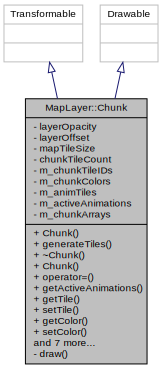
\includegraphics[width=235pt]{classMapLayer_1_1Chunk__inherit__graph}
\end{center}
\end{figure}


Collaboration diagram for Map\+Layer\+:\+:Chunk\+:
\nopagebreak
\begin{figure}[H]
\begin{center}
\leavevmode
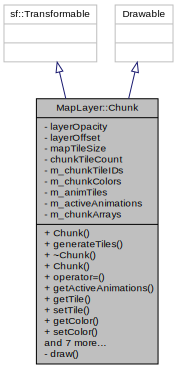
\includegraphics[width=235pt]{classMapLayer_1_1Chunk__coll__graph}
\end{center}
\end{figure}
\subsection*{Classes}
\begin{DoxyCompactItemize}
\item 
class \hyperlink{classMapLayer_1_1Chunk_1_1ChunkArray}{Chunk\+Array}
\end{DoxyCompactItemize}
\subsection*{Public Types}
\begin{DoxyCompactItemize}
\item 
using \hyperlink{classMapLayer_1_1Chunk_ab1df4d3621c5d9f83c2edb46d0744078}{Ptr} = std\+::unique\+\_\+ptr$<$ \hyperlink{classMapLayer_1_1Chunk}{Chunk} $>$
\item 
using \hyperlink{classMapLayer_1_1Chunk_a2137a288bfd4120eb3e4db5934b802f3}{Tile} = std\+::array$<$ sf\+::\+Vertex, 4u $>$
\end{DoxyCompactItemize}
\subsection*{Public Member Functions}
\begin{DoxyCompactItemize}
\item 
\hyperlink{classMapLayer_1_1Chunk_a793a265040a7e0e117d47463b5d1f762}{Chunk} (const tmx\+::\+Tile\+Layer \&layer, std\+::vector$<$ const tmx\+::\+Tileset $\ast$$>$ tilesets, const sf\+::\+Vector2f \&position, const sf\+::\+Vector2f \&tile\+Count, const sf\+::\+Vector2u \&tile\+Size, std\+::size\+\_\+t row\+Size, \hyperlink{classMapLayer_a64011087426e436e3cb8374570378d68}{Texture\+Resource} \&tr, const std\+::map$<$ std\+::uint32\+\_\+t, tmx\+::\+Tileset\+::\+Tile $>$ \&anim\+Tiles)
\item 
void \hyperlink{classMapLayer_1_1Chunk_aa8e16ad1e2e77a00313c4ed92f0a87b7}{generate\+Tiles} (bool register\+Animation=false)
\item 
\hyperlink{classMapLayer_1_1Chunk_a868f8750a2139ead6a79ae6f228303f5}{$\sim$\+Chunk} ()=default
\item 
\hyperlink{classMapLayer_1_1Chunk_ad135fca4082657b3babebd9c5b3402a8}{Chunk} (const \hyperlink{classMapLayer_1_1Chunk}{Chunk} \&)=delete
\item 
\hyperlink{classMapLayer_1_1Chunk}{Chunk} \& \hyperlink{classMapLayer_1_1Chunk_aad57eee35df69297877377ac64dceb6f}{operator=} (const \hyperlink{classMapLayer_1_1Chunk}{Chunk} \&)=delete
\item 
std\+::vector$<$ \hyperlink{structMapLayer_1_1AnimationState}{Animation\+State} $>$ \& \hyperlink{classMapLayer_1_1Chunk_adc0fdad3f30d7ff327b2a538efc8c949}{get\+Active\+Animations} ()
\item 
tmx\+::\+Tile\+Layer\+::\+Tile \hyperlink{classMapLayer_1_1Chunk_ae70972baf5ed18a69709f180e62f4eb5}{get\+Tile} (int x, int y) const
\item 
void \hyperlink{classMapLayer_1_1Chunk_a557343f1e955e78b6f68623007fb9a7a}{set\+Tile} (int x, int y, tmx\+::\+Tile\+Layer\+::\+Tile tile, bool refresh)
\item 
sf\+::\+Color \hyperlink{classMapLayer_1_1Chunk_aeee5ad34f7c428e1fd290b2a1a695397}{get\+Color} (int x, int y) const
\item 
void \hyperlink{classMapLayer_1_1Chunk_addf26b112e46bc6995f03a886cf46dc8}{set\+Color} (int x, int y, sf\+::\+Color color, bool refresh)
\item 
void \hyperlink{classMapLayer_1_1Chunk_abf755ab4f7b9430aae29a631eb2ee48e}{maybe\+Regenerate} (bool refresh)
\item 
int \hyperlink{classMapLayer_1_1Chunk_a3df37cf62d435f242780c6ae3cf0f339}{calc\+Index\+From} (int x, int y) const
\item 
bool \hyperlink{classMapLayer_1_1Chunk_ad7e91d957e932e8c4235f5008cbd03c8}{empty} () const
\item 
void \hyperlink{classMapLayer_1_1Chunk_a6de781e426b23c3b33e34a1ea70eb14f}{flipY} (sf\+::\+Vector2f $\ast$v0, sf\+::\+Vector2f $\ast$v1, sf\+::\+Vector2f $\ast$v2, sf\+::\+Vector2f $\ast$v3)
\item 
void \hyperlink{classMapLayer_1_1Chunk_a0bd785f9c54b97ae99417261210b9579}{flipX} (sf\+::\+Vector2f $\ast$v0, sf\+::\+Vector2f $\ast$v1, sf\+::\+Vector2f $\ast$v2, sf\+::\+Vector2f $\ast$v3)
\item 
void \hyperlink{classMapLayer_1_1Chunk_a82346cb03113d15eb2b135c082257b0e}{flipD} (sf\+::\+Vector2f $\ast$v0, sf\+::\+Vector2f $\ast$v1, sf\+::\+Vector2f $\ast$v2, sf\+::\+Vector2f $\ast$v3)
\item 
void \hyperlink{classMapLayer_1_1Chunk_ac90c3c9041c12cf6955707966c20d0cc}{do\+Flips} (std\+::uint8\+\_\+t bits, sf\+::\+Vector2f $\ast$v0, sf\+::\+Vector2f $\ast$v1, sf\+::\+Vector2f $\ast$v2, sf\+::\+Vector2f $\ast$v3)
\end{DoxyCompactItemize}
\subsection*{Private Member Functions}
\begin{DoxyCompactItemize}
\item 
void \hyperlink{classMapLayer_1_1Chunk_ab2f932fad581f2dd23d1570ebb4c76b9}{draw} (sf\+::\+Render\+Target \&rt, sf\+::\+Render\+States states) const override
\end{DoxyCompactItemize}
\subsection*{Private Attributes}
\begin{DoxyCompactItemize}
\item 
sf\+::\+Uint8 \hyperlink{classMapLayer_1_1Chunk_a2540be672f38d7f6826eebb944881429}{layer\+Opacity}
\item 
sf\+::\+Vector2f \hyperlink{classMapLayer_1_1Chunk_a58aafb7ea1d939755673bef91bfe313e}{layer\+Offset}
\item 
sf\+::\+Vector2u \hyperlink{classMapLayer_1_1Chunk_a010215bc42e515278da75b680c88dcdf}{map\+Tile\+Size}
\item 
sf\+::\+Vector2f \hyperlink{classMapLayer_1_1Chunk_a48d8fc51f7358f229818659ae7869485}{chunk\+Tile\+Count}
\item 
std\+::vector$<$ tmx\+::\+Tile\+Layer\+::\+Tile $>$ \hyperlink{classMapLayer_1_1Chunk_ab40e4c80d3c205fc62db6a1c90e6afe7}{m\+\_\+chunk\+Tile\+I\+Ds}
\item 
std\+::vector$<$ sf\+::\+Color $>$ \hyperlink{classMapLayer_1_1Chunk_ab09b61a5d77f4acad152ac60db3cd333}{m\+\_\+chunk\+Colors}
\item 
std\+::map$<$ std\+::uint32\+\_\+t, tmx\+::\+Tileset\+::\+Tile $>$ \hyperlink{classMapLayer_1_1Chunk_a70854589957a8232358b04f971c1a1ec}{m\+\_\+anim\+Tiles}
\item 
std\+::vector$<$ \hyperlink{structMapLayer_1_1AnimationState}{Animation\+State} $>$ \hyperlink{classMapLayer_1_1Chunk_a8b618ddd7286a02a668fb9f8404427b6}{m\+\_\+active\+Animations}
\item 
std\+::vector$<$ \hyperlink{classMapLayer_1_1Chunk_1_1ChunkArray_a6d944dee2fc89a76d7a252405e2732b0}{Chunk\+Array\+::\+Ptr} $>$ \hyperlink{classMapLayer_1_1Chunk_ab264049d7a576a9b8efd88df159704bf}{m\+\_\+chunk\+Arrays}
\end{DoxyCompactItemize}


\subsection{Member Typedef Documentation}
\mbox{\Hypertarget{classMapLayer_1_1Chunk_ab1df4d3621c5d9f83c2edb46d0744078}\label{classMapLayer_1_1Chunk_ab1df4d3621c5d9f83c2edb46d0744078}} 
\index{Map\+Layer\+::\+Chunk@{Map\+Layer\+::\+Chunk}!Ptr@{Ptr}}
\index{Ptr@{Ptr}!Map\+Layer\+::\+Chunk@{Map\+Layer\+::\+Chunk}}
\subsubsection{\texorpdfstring{Ptr}{Ptr}}
{\footnotesize\ttfamily using \hyperlink{classMapLayer_1_1Chunk_ab1df4d3621c5d9f83c2edb46d0744078}{Map\+Layer\+::\+Chunk\+::\+Ptr} =  std\+::unique\+\_\+ptr$<$\hyperlink{classMapLayer_1_1Chunk}{Chunk}$>$}

\mbox{\Hypertarget{classMapLayer_1_1Chunk_a2137a288bfd4120eb3e4db5934b802f3}\label{classMapLayer_1_1Chunk_a2137a288bfd4120eb3e4db5934b802f3}} 
\index{Map\+Layer\+::\+Chunk@{Map\+Layer\+::\+Chunk}!Tile@{Tile}}
\index{Tile@{Tile}!Map\+Layer\+::\+Chunk@{Map\+Layer\+::\+Chunk}}
\subsubsection{\texorpdfstring{Tile}{Tile}}
{\footnotesize\ttfamily using \hyperlink{classMapLayer_1_1Chunk_a2137a288bfd4120eb3e4db5934b802f3}{Map\+Layer\+::\+Chunk\+::\+Tile} =  std\+::array$<$sf\+::\+Vertex, 4u$>$}



\subsection{Constructor \& Destructor Documentation}
\mbox{\Hypertarget{classMapLayer_1_1Chunk_a793a265040a7e0e117d47463b5d1f762}\label{classMapLayer_1_1Chunk_a793a265040a7e0e117d47463b5d1f762}} 
\index{Map\+Layer\+::\+Chunk@{Map\+Layer\+::\+Chunk}!Chunk@{Chunk}}
\index{Chunk@{Chunk}!Map\+Layer\+::\+Chunk@{Map\+Layer\+::\+Chunk}}
\subsubsection{\texorpdfstring{Chunk()}{Chunk()}\hspace{0.1cm}{\footnotesize\ttfamily [1/2]}}
{\footnotesize\ttfamily Map\+Layer\+::\+Chunk\+::\+Chunk (\begin{DoxyParamCaption}\item[{const tmx\+::\+Tile\+Layer \&}]{layer,  }\item[{std\+::vector$<$ const tmx\+::\+Tileset $\ast$$>$}]{tilesets,  }\item[{const sf\+::\+Vector2f \&}]{position,  }\item[{const sf\+::\+Vector2f \&}]{tile\+Count,  }\item[{const sf\+::\+Vector2u \&}]{tile\+Size,  }\item[{std\+::size\+\_\+t}]{row\+Size,  }\item[{\hyperlink{classMapLayer_a64011087426e436e3cb8374570378d68}{Texture\+Resource} \&}]{tr,  }\item[{const std\+::map$<$ std\+::uint32\+\_\+t, tmx\+::\+Tileset\+::\+Tile $>$ \&}]{anim\+Tiles }\end{DoxyParamCaption})\hspace{0.3cm}{\ttfamily [inline]}}

\mbox{\Hypertarget{classMapLayer_1_1Chunk_a868f8750a2139ead6a79ae6f228303f5}\label{classMapLayer_1_1Chunk_a868f8750a2139ead6a79ae6f228303f5}} 
\index{Map\+Layer\+::\+Chunk@{Map\+Layer\+::\+Chunk}!````~Chunk@{$\sim$\+Chunk}}
\index{````~Chunk@{$\sim$\+Chunk}!Map\+Layer\+::\+Chunk@{Map\+Layer\+::\+Chunk}}
\subsubsection{\texorpdfstring{$\sim$\+Chunk()}{~Chunk()}}
{\footnotesize\ttfamily Map\+Layer\+::\+Chunk\+::$\sim$\+Chunk (\begin{DoxyParamCaption}{ }\end{DoxyParamCaption})\hspace{0.3cm}{\ttfamily [default]}}

\mbox{\Hypertarget{classMapLayer_1_1Chunk_ad135fca4082657b3babebd9c5b3402a8}\label{classMapLayer_1_1Chunk_ad135fca4082657b3babebd9c5b3402a8}} 
\index{Map\+Layer\+::\+Chunk@{Map\+Layer\+::\+Chunk}!Chunk@{Chunk}}
\index{Chunk@{Chunk}!Map\+Layer\+::\+Chunk@{Map\+Layer\+::\+Chunk}}
\subsubsection{\texorpdfstring{Chunk()}{Chunk()}\hspace{0.1cm}{\footnotesize\ttfamily [2/2]}}
{\footnotesize\ttfamily Map\+Layer\+::\+Chunk\+::\+Chunk (\begin{DoxyParamCaption}\item[{const \hyperlink{classMapLayer_1_1Chunk}{Chunk} \&}]{ }\end{DoxyParamCaption})\hspace{0.3cm}{\ttfamily [delete]}}



\subsection{Member Function Documentation}
\mbox{\Hypertarget{classMapLayer_1_1Chunk_a3df37cf62d435f242780c6ae3cf0f339}\label{classMapLayer_1_1Chunk_a3df37cf62d435f242780c6ae3cf0f339}} 
\index{Map\+Layer\+::\+Chunk@{Map\+Layer\+::\+Chunk}!calc\+Index\+From@{calc\+Index\+From}}
\index{calc\+Index\+From@{calc\+Index\+From}!Map\+Layer\+::\+Chunk@{Map\+Layer\+::\+Chunk}}
\subsubsection{\texorpdfstring{calc\+Index\+From()}{calcIndexFrom()}}
{\footnotesize\ttfamily int Map\+Layer\+::\+Chunk\+::calc\+Index\+From (\begin{DoxyParamCaption}\item[{int}]{x,  }\item[{int}]{y }\end{DoxyParamCaption}) const\hspace{0.3cm}{\ttfamily [inline]}}

\mbox{\Hypertarget{classMapLayer_1_1Chunk_ac90c3c9041c12cf6955707966c20d0cc}\label{classMapLayer_1_1Chunk_ac90c3c9041c12cf6955707966c20d0cc}} 
\index{Map\+Layer\+::\+Chunk@{Map\+Layer\+::\+Chunk}!do\+Flips@{do\+Flips}}
\index{do\+Flips@{do\+Flips}!Map\+Layer\+::\+Chunk@{Map\+Layer\+::\+Chunk}}
\subsubsection{\texorpdfstring{do\+Flips()}{doFlips()}}
{\footnotesize\ttfamily void Map\+Layer\+::\+Chunk\+::do\+Flips (\begin{DoxyParamCaption}\item[{std\+::uint8\+\_\+t}]{bits,  }\item[{sf\+::\+Vector2f $\ast$}]{v0,  }\item[{sf\+::\+Vector2f $\ast$}]{v1,  }\item[{sf\+::\+Vector2f $\ast$}]{v2,  }\item[{sf\+::\+Vector2f $\ast$}]{v3 }\end{DoxyParamCaption})\hspace{0.3cm}{\ttfamily [inline]}}

\mbox{\Hypertarget{classMapLayer_1_1Chunk_ab2f932fad581f2dd23d1570ebb4c76b9}\label{classMapLayer_1_1Chunk_ab2f932fad581f2dd23d1570ebb4c76b9}} 
\index{Map\+Layer\+::\+Chunk@{Map\+Layer\+::\+Chunk}!draw@{draw}}
\index{draw@{draw}!Map\+Layer\+::\+Chunk@{Map\+Layer\+::\+Chunk}}
\subsubsection{\texorpdfstring{draw()}{draw()}}
{\footnotesize\ttfamily void Map\+Layer\+::\+Chunk\+::draw (\begin{DoxyParamCaption}\item[{sf\+::\+Render\+Target \&}]{rt,  }\item[{sf\+::\+Render\+States}]{states }\end{DoxyParamCaption}) const\hspace{0.3cm}{\ttfamily [inline]}, {\ttfamily [override]}, {\ttfamily [private]}}

\mbox{\Hypertarget{classMapLayer_1_1Chunk_ad7e91d957e932e8c4235f5008cbd03c8}\label{classMapLayer_1_1Chunk_ad7e91d957e932e8c4235f5008cbd03c8}} 
\index{Map\+Layer\+::\+Chunk@{Map\+Layer\+::\+Chunk}!empty@{empty}}
\index{empty@{empty}!Map\+Layer\+::\+Chunk@{Map\+Layer\+::\+Chunk}}
\subsubsection{\texorpdfstring{empty()}{empty()}}
{\footnotesize\ttfamily bool Map\+Layer\+::\+Chunk\+::empty (\begin{DoxyParamCaption}{ }\end{DoxyParamCaption}) const\hspace{0.3cm}{\ttfamily [inline]}}

\mbox{\Hypertarget{classMapLayer_1_1Chunk_a82346cb03113d15eb2b135c082257b0e}\label{classMapLayer_1_1Chunk_a82346cb03113d15eb2b135c082257b0e}} 
\index{Map\+Layer\+::\+Chunk@{Map\+Layer\+::\+Chunk}!flipD@{flipD}}
\index{flipD@{flipD}!Map\+Layer\+::\+Chunk@{Map\+Layer\+::\+Chunk}}
\subsubsection{\texorpdfstring{flip\+D()}{flipD()}}
{\footnotesize\ttfamily void Map\+Layer\+::\+Chunk\+::flipD (\begin{DoxyParamCaption}\item[{sf\+::\+Vector2f $\ast$}]{v0,  }\item[{sf\+::\+Vector2f $\ast$}]{v1,  }\item[{sf\+::\+Vector2f $\ast$}]{v2,  }\item[{sf\+::\+Vector2f $\ast$}]{v3 }\end{DoxyParamCaption})\hspace{0.3cm}{\ttfamily [inline]}}

\mbox{\Hypertarget{classMapLayer_1_1Chunk_a0bd785f9c54b97ae99417261210b9579}\label{classMapLayer_1_1Chunk_a0bd785f9c54b97ae99417261210b9579}} 
\index{Map\+Layer\+::\+Chunk@{Map\+Layer\+::\+Chunk}!flipX@{flipX}}
\index{flipX@{flipX}!Map\+Layer\+::\+Chunk@{Map\+Layer\+::\+Chunk}}
\subsubsection{\texorpdfstring{flip\+X()}{flipX()}}
{\footnotesize\ttfamily void Map\+Layer\+::\+Chunk\+::flipX (\begin{DoxyParamCaption}\item[{sf\+::\+Vector2f $\ast$}]{v0,  }\item[{sf\+::\+Vector2f $\ast$}]{v1,  }\item[{sf\+::\+Vector2f $\ast$}]{v2,  }\item[{sf\+::\+Vector2f $\ast$}]{v3 }\end{DoxyParamCaption})\hspace{0.3cm}{\ttfamily [inline]}}

\mbox{\Hypertarget{classMapLayer_1_1Chunk_a6de781e426b23c3b33e34a1ea70eb14f}\label{classMapLayer_1_1Chunk_a6de781e426b23c3b33e34a1ea70eb14f}} 
\index{Map\+Layer\+::\+Chunk@{Map\+Layer\+::\+Chunk}!flipY@{flipY}}
\index{flipY@{flipY}!Map\+Layer\+::\+Chunk@{Map\+Layer\+::\+Chunk}}
\subsubsection{\texorpdfstring{flip\+Y()}{flipY()}}
{\footnotesize\ttfamily void Map\+Layer\+::\+Chunk\+::flipY (\begin{DoxyParamCaption}\item[{sf\+::\+Vector2f $\ast$}]{v0,  }\item[{sf\+::\+Vector2f $\ast$}]{v1,  }\item[{sf\+::\+Vector2f $\ast$}]{v2,  }\item[{sf\+::\+Vector2f $\ast$}]{v3 }\end{DoxyParamCaption})\hspace{0.3cm}{\ttfamily [inline]}}

\mbox{\Hypertarget{classMapLayer_1_1Chunk_aa8e16ad1e2e77a00313c4ed92f0a87b7}\label{classMapLayer_1_1Chunk_aa8e16ad1e2e77a00313c4ed92f0a87b7}} 
\index{Map\+Layer\+::\+Chunk@{Map\+Layer\+::\+Chunk}!generate\+Tiles@{generate\+Tiles}}
\index{generate\+Tiles@{generate\+Tiles}!Map\+Layer\+::\+Chunk@{Map\+Layer\+::\+Chunk}}
\subsubsection{\texorpdfstring{generate\+Tiles()}{generateTiles()}}
{\footnotesize\ttfamily void Map\+Layer\+::\+Chunk\+::generate\+Tiles (\begin{DoxyParamCaption}\item[{bool}]{register\+Animation = {\ttfamily false} }\end{DoxyParamCaption})\hspace{0.3cm}{\ttfamily [inline]}}

\mbox{\Hypertarget{classMapLayer_1_1Chunk_adc0fdad3f30d7ff327b2a538efc8c949}\label{classMapLayer_1_1Chunk_adc0fdad3f30d7ff327b2a538efc8c949}} 
\index{Map\+Layer\+::\+Chunk@{Map\+Layer\+::\+Chunk}!get\+Active\+Animations@{get\+Active\+Animations}}
\index{get\+Active\+Animations@{get\+Active\+Animations}!Map\+Layer\+::\+Chunk@{Map\+Layer\+::\+Chunk}}
\subsubsection{\texorpdfstring{get\+Active\+Animations()}{getActiveAnimations()}}
{\footnotesize\ttfamily std\+::vector$<$\hyperlink{structMapLayer_1_1AnimationState}{Animation\+State}$>$\& Map\+Layer\+::\+Chunk\+::get\+Active\+Animations (\begin{DoxyParamCaption}{ }\end{DoxyParamCaption})\hspace{0.3cm}{\ttfamily [inline]}}

\mbox{\Hypertarget{classMapLayer_1_1Chunk_aeee5ad34f7c428e1fd290b2a1a695397}\label{classMapLayer_1_1Chunk_aeee5ad34f7c428e1fd290b2a1a695397}} 
\index{Map\+Layer\+::\+Chunk@{Map\+Layer\+::\+Chunk}!get\+Color@{get\+Color}}
\index{get\+Color@{get\+Color}!Map\+Layer\+::\+Chunk@{Map\+Layer\+::\+Chunk}}
\subsubsection{\texorpdfstring{get\+Color()}{getColor()}}
{\footnotesize\ttfamily sf\+::\+Color Map\+Layer\+::\+Chunk\+::get\+Color (\begin{DoxyParamCaption}\item[{int}]{x,  }\item[{int}]{y }\end{DoxyParamCaption}) const\hspace{0.3cm}{\ttfamily [inline]}}

\mbox{\Hypertarget{classMapLayer_1_1Chunk_ae70972baf5ed18a69709f180e62f4eb5}\label{classMapLayer_1_1Chunk_ae70972baf5ed18a69709f180e62f4eb5}} 
\index{Map\+Layer\+::\+Chunk@{Map\+Layer\+::\+Chunk}!get\+Tile@{get\+Tile}}
\index{get\+Tile@{get\+Tile}!Map\+Layer\+::\+Chunk@{Map\+Layer\+::\+Chunk}}
\subsubsection{\texorpdfstring{get\+Tile()}{getTile()}}
{\footnotesize\ttfamily tmx\+::\+Tile\+Layer\+::\+Tile Map\+Layer\+::\+Chunk\+::get\+Tile (\begin{DoxyParamCaption}\item[{int}]{x,  }\item[{int}]{y }\end{DoxyParamCaption}) const\hspace{0.3cm}{\ttfamily [inline]}}

\mbox{\Hypertarget{classMapLayer_1_1Chunk_abf755ab4f7b9430aae29a631eb2ee48e}\label{classMapLayer_1_1Chunk_abf755ab4f7b9430aae29a631eb2ee48e}} 
\index{Map\+Layer\+::\+Chunk@{Map\+Layer\+::\+Chunk}!maybe\+Regenerate@{maybe\+Regenerate}}
\index{maybe\+Regenerate@{maybe\+Regenerate}!Map\+Layer\+::\+Chunk@{Map\+Layer\+::\+Chunk}}
\subsubsection{\texorpdfstring{maybe\+Regenerate()}{maybeRegenerate()}}
{\footnotesize\ttfamily void Map\+Layer\+::\+Chunk\+::maybe\+Regenerate (\begin{DoxyParamCaption}\item[{bool}]{refresh }\end{DoxyParamCaption})\hspace{0.3cm}{\ttfamily [inline]}}

\mbox{\Hypertarget{classMapLayer_1_1Chunk_aad57eee35df69297877377ac64dceb6f}\label{classMapLayer_1_1Chunk_aad57eee35df69297877377ac64dceb6f}} 
\index{Map\+Layer\+::\+Chunk@{Map\+Layer\+::\+Chunk}!operator=@{operator=}}
\index{operator=@{operator=}!Map\+Layer\+::\+Chunk@{Map\+Layer\+::\+Chunk}}
\subsubsection{\texorpdfstring{operator=()}{operator=()}}
{\footnotesize\ttfamily \hyperlink{classMapLayer_1_1Chunk}{Chunk}\& Map\+Layer\+::\+Chunk\+::operator= (\begin{DoxyParamCaption}\item[{const \hyperlink{classMapLayer_1_1Chunk}{Chunk} \&}]{ }\end{DoxyParamCaption})\hspace{0.3cm}{\ttfamily [delete]}}

\mbox{\Hypertarget{classMapLayer_1_1Chunk_addf26b112e46bc6995f03a886cf46dc8}\label{classMapLayer_1_1Chunk_addf26b112e46bc6995f03a886cf46dc8}} 
\index{Map\+Layer\+::\+Chunk@{Map\+Layer\+::\+Chunk}!set\+Color@{set\+Color}}
\index{set\+Color@{set\+Color}!Map\+Layer\+::\+Chunk@{Map\+Layer\+::\+Chunk}}
\subsubsection{\texorpdfstring{set\+Color()}{setColor()}}
{\footnotesize\ttfamily void Map\+Layer\+::\+Chunk\+::set\+Color (\begin{DoxyParamCaption}\item[{int}]{x,  }\item[{int}]{y,  }\item[{sf\+::\+Color}]{color,  }\item[{bool}]{refresh }\end{DoxyParamCaption})\hspace{0.3cm}{\ttfamily [inline]}}

\mbox{\Hypertarget{classMapLayer_1_1Chunk_a557343f1e955e78b6f68623007fb9a7a}\label{classMapLayer_1_1Chunk_a557343f1e955e78b6f68623007fb9a7a}} 
\index{Map\+Layer\+::\+Chunk@{Map\+Layer\+::\+Chunk}!set\+Tile@{set\+Tile}}
\index{set\+Tile@{set\+Tile}!Map\+Layer\+::\+Chunk@{Map\+Layer\+::\+Chunk}}
\subsubsection{\texorpdfstring{set\+Tile()}{setTile()}}
{\footnotesize\ttfamily void Map\+Layer\+::\+Chunk\+::set\+Tile (\begin{DoxyParamCaption}\item[{int}]{x,  }\item[{int}]{y,  }\item[{tmx\+::\+Tile\+Layer\+::\+Tile}]{tile,  }\item[{bool}]{refresh }\end{DoxyParamCaption})\hspace{0.3cm}{\ttfamily [inline]}}



\subsection{Member Data Documentation}
\mbox{\Hypertarget{classMapLayer_1_1Chunk_a48d8fc51f7358f229818659ae7869485}\label{classMapLayer_1_1Chunk_a48d8fc51f7358f229818659ae7869485}} 
\index{Map\+Layer\+::\+Chunk@{Map\+Layer\+::\+Chunk}!chunk\+Tile\+Count@{chunk\+Tile\+Count}}
\index{chunk\+Tile\+Count@{chunk\+Tile\+Count}!Map\+Layer\+::\+Chunk@{Map\+Layer\+::\+Chunk}}
\subsubsection{\texorpdfstring{chunk\+Tile\+Count}{chunkTileCount}}
{\footnotesize\ttfamily sf\+::\+Vector2f Map\+Layer\+::\+Chunk\+::chunk\+Tile\+Count\hspace{0.3cm}{\ttfamily [private]}}

\mbox{\Hypertarget{classMapLayer_1_1Chunk_a58aafb7ea1d939755673bef91bfe313e}\label{classMapLayer_1_1Chunk_a58aafb7ea1d939755673bef91bfe313e}} 
\index{Map\+Layer\+::\+Chunk@{Map\+Layer\+::\+Chunk}!layer\+Offset@{layer\+Offset}}
\index{layer\+Offset@{layer\+Offset}!Map\+Layer\+::\+Chunk@{Map\+Layer\+::\+Chunk}}
\subsubsection{\texorpdfstring{layer\+Offset}{layerOffset}}
{\footnotesize\ttfamily sf\+::\+Vector2f Map\+Layer\+::\+Chunk\+::layer\+Offset\hspace{0.3cm}{\ttfamily [private]}}

\mbox{\Hypertarget{classMapLayer_1_1Chunk_a2540be672f38d7f6826eebb944881429}\label{classMapLayer_1_1Chunk_a2540be672f38d7f6826eebb944881429}} 
\index{Map\+Layer\+::\+Chunk@{Map\+Layer\+::\+Chunk}!layer\+Opacity@{layer\+Opacity}}
\index{layer\+Opacity@{layer\+Opacity}!Map\+Layer\+::\+Chunk@{Map\+Layer\+::\+Chunk}}
\subsubsection{\texorpdfstring{layer\+Opacity}{layerOpacity}}
{\footnotesize\ttfamily sf\+::\+Uint8 Map\+Layer\+::\+Chunk\+::layer\+Opacity\hspace{0.3cm}{\ttfamily [private]}}

\mbox{\Hypertarget{classMapLayer_1_1Chunk_a8b618ddd7286a02a668fb9f8404427b6}\label{classMapLayer_1_1Chunk_a8b618ddd7286a02a668fb9f8404427b6}} 
\index{Map\+Layer\+::\+Chunk@{Map\+Layer\+::\+Chunk}!m\+\_\+active\+Animations@{m\+\_\+active\+Animations}}
\index{m\+\_\+active\+Animations@{m\+\_\+active\+Animations}!Map\+Layer\+::\+Chunk@{Map\+Layer\+::\+Chunk}}
\subsubsection{\texorpdfstring{m\+\_\+active\+Animations}{m\_activeAnimations}}
{\footnotesize\ttfamily std\+::vector$<$\hyperlink{structMapLayer_1_1AnimationState}{Animation\+State}$>$ Map\+Layer\+::\+Chunk\+::m\+\_\+active\+Animations\hspace{0.3cm}{\ttfamily [private]}}

\mbox{\Hypertarget{classMapLayer_1_1Chunk_a70854589957a8232358b04f971c1a1ec}\label{classMapLayer_1_1Chunk_a70854589957a8232358b04f971c1a1ec}} 
\index{Map\+Layer\+::\+Chunk@{Map\+Layer\+::\+Chunk}!m\+\_\+anim\+Tiles@{m\+\_\+anim\+Tiles}}
\index{m\+\_\+anim\+Tiles@{m\+\_\+anim\+Tiles}!Map\+Layer\+::\+Chunk@{Map\+Layer\+::\+Chunk}}
\subsubsection{\texorpdfstring{m\+\_\+anim\+Tiles}{m\_animTiles}}
{\footnotesize\ttfamily std\+::map$<$std\+::uint32\+\_\+t, tmx\+::\+Tileset\+::\+Tile$>$ Map\+Layer\+::\+Chunk\+::m\+\_\+anim\+Tiles\hspace{0.3cm}{\ttfamily [private]}}

\mbox{\Hypertarget{classMapLayer_1_1Chunk_ab264049d7a576a9b8efd88df159704bf}\label{classMapLayer_1_1Chunk_ab264049d7a576a9b8efd88df159704bf}} 
\index{Map\+Layer\+::\+Chunk@{Map\+Layer\+::\+Chunk}!m\+\_\+chunk\+Arrays@{m\+\_\+chunk\+Arrays}}
\index{m\+\_\+chunk\+Arrays@{m\+\_\+chunk\+Arrays}!Map\+Layer\+::\+Chunk@{Map\+Layer\+::\+Chunk}}
\subsubsection{\texorpdfstring{m\+\_\+chunk\+Arrays}{m\_chunkArrays}}
{\footnotesize\ttfamily std\+::vector$<$\hyperlink{classMapLayer_1_1Chunk_1_1ChunkArray_a6d944dee2fc89a76d7a252405e2732b0}{Chunk\+Array\+::\+Ptr}$>$ Map\+Layer\+::\+Chunk\+::m\+\_\+chunk\+Arrays\hspace{0.3cm}{\ttfamily [private]}}

\mbox{\Hypertarget{classMapLayer_1_1Chunk_ab09b61a5d77f4acad152ac60db3cd333}\label{classMapLayer_1_1Chunk_ab09b61a5d77f4acad152ac60db3cd333}} 
\index{Map\+Layer\+::\+Chunk@{Map\+Layer\+::\+Chunk}!m\+\_\+chunk\+Colors@{m\+\_\+chunk\+Colors}}
\index{m\+\_\+chunk\+Colors@{m\+\_\+chunk\+Colors}!Map\+Layer\+::\+Chunk@{Map\+Layer\+::\+Chunk}}
\subsubsection{\texorpdfstring{m\+\_\+chunk\+Colors}{m\_chunkColors}}
{\footnotesize\ttfamily std\+::vector$<$sf\+::\+Color$>$ Map\+Layer\+::\+Chunk\+::m\+\_\+chunk\+Colors\hspace{0.3cm}{\ttfamily [private]}}

\mbox{\Hypertarget{classMapLayer_1_1Chunk_ab40e4c80d3c205fc62db6a1c90e6afe7}\label{classMapLayer_1_1Chunk_ab40e4c80d3c205fc62db6a1c90e6afe7}} 
\index{Map\+Layer\+::\+Chunk@{Map\+Layer\+::\+Chunk}!m\+\_\+chunk\+Tile\+I\+Ds@{m\+\_\+chunk\+Tile\+I\+Ds}}
\index{m\+\_\+chunk\+Tile\+I\+Ds@{m\+\_\+chunk\+Tile\+I\+Ds}!Map\+Layer\+::\+Chunk@{Map\+Layer\+::\+Chunk}}
\subsubsection{\texorpdfstring{m\+\_\+chunk\+Tile\+I\+Ds}{m\_chunkTileIDs}}
{\footnotesize\ttfamily std\+::vector$<$tmx\+::\+Tile\+Layer\+::\+Tile$>$ Map\+Layer\+::\+Chunk\+::m\+\_\+chunk\+Tile\+I\+Ds\hspace{0.3cm}{\ttfamily [private]}}

\mbox{\Hypertarget{classMapLayer_1_1Chunk_a010215bc42e515278da75b680c88dcdf}\label{classMapLayer_1_1Chunk_a010215bc42e515278da75b680c88dcdf}} 
\index{Map\+Layer\+::\+Chunk@{Map\+Layer\+::\+Chunk}!map\+Tile\+Size@{map\+Tile\+Size}}
\index{map\+Tile\+Size@{map\+Tile\+Size}!Map\+Layer\+::\+Chunk@{Map\+Layer\+::\+Chunk}}
\subsubsection{\texorpdfstring{map\+Tile\+Size}{mapTileSize}}
{\footnotesize\ttfamily sf\+::\+Vector2u Map\+Layer\+::\+Chunk\+::map\+Tile\+Size\hspace{0.3cm}{\ttfamily [private]}}



The documentation for this class was generated from the following file\+:\begin{DoxyCompactItemize}
\item 
/mnt/hdd/\+C0de/\+Engines/\+S\+F\+M\+L/\+S\+F\+M\+L\+\_\+\+Engine/include/\hyperlink{SFMLOrthogonalLayer_8hpp}{S\+F\+M\+L\+Orthogonal\+Layer.\+hpp}\end{DoxyCompactItemize}

\hypertarget{classMapLayer_1_1Chunk_1_1ChunkArray}{}\section{Map\+Layer\+:\+:Chunk\+:\+:Chunk\+Array Class Reference}
\label{classMapLayer_1_1Chunk_1_1ChunkArray}\index{Map\+Layer\+::\+Chunk\+::\+Chunk\+Array@{Map\+Layer\+::\+Chunk\+::\+Chunk\+Array}}


Inheritance diagram for Map\+Layer\+:\+:Chunk\+:\+:Chunk\+Array\+:
\nopagebreak
\begin{figure}[H]
\begin{center}
\leavevmode
\includegraphics[width=232pt]{classMapLayer_1_1Chunk_1_1ChunkArray__inherit__graph}
\end{center}
\end{figure}


Collaboration diagram for Map\+Layer\+:\+:Chunk\+:\+:Chunk\+Array\+:
\nopagebreak
\begin{figure}[H]
\begin{center}
\leavevmode
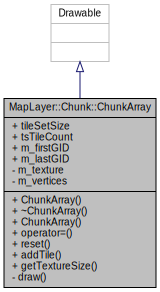
\includegraphics[width=232pt]{classMapLayer_1_1Chunk_1_1ChunkArray__coll__graph}
\end{center}
\end{figure}
\subsection*{Public Types}
\begin{DoxyCompactItemize}
\item 
using \hyperlink{classMapLayer_1_1Chunk_1_1ChunkArray_a6d944dee2fc89a76d7a252405e2732b0}{Ptr} = std\+::unique\+\_\+ptr$<$ \hyperlink{classMapLayer_1_1Chunk_1_1ChunkArray}{Chunk\+Array} $>$
\end{DoxyCompactItemize}
\subsection*{Public Member Functions}
\begin{DoxyCompactItemize}
\item 
\hyperlink{classMapLayer_1_1Chunk_1_1ChunkArray_a566f7f2c8c1fd2405ed8a359a9cf8717}{Chunk\+Array} (const sf\+::\+Texture \&t, const tmx\+::\+Tileset \&ts)
\item 
\hyperlink{classMapLayer_1_1Chunk_1_1ChunkArray_a032e0fa8a35d86815109eb0e1296c567}{$\sim$\+Chunk\+Array} ()=default
\item 
\hyperlink{classMapLayer_1_1Chunk_1_1ChunkArray_a85a82c50eae1a835b7a355813b560cbf}{Chunk\+Array} (const \hyperlink{classMapLayer_1_1Chunk_1_1ChunkArray}{Chunk\+Array} \&)=delete
\item 
\hyperlink{classMapLayer_1_1Chunk_1_1ChunkArray}{Chunk\+Array} \& \hyperlink{classMapLayer_1_1Chunk_1_1ChunkArray_ad5c7843e61bbddfb1be30ec93d75510f}{operator=} (const \hyperlink{classMapLayer_1_1Chunk_1_1ChunkArray}{Chunk\+Array} \&)=delete
\item 
void \hyperlink{classMapLayer_1_1Chunk_1_1ChunkArray_a4f93efce951889766d0336525e697cdd}{reset} ()
\item 
void \hyperlink{classMapLayer_1_1Chunk_1_1ChunkArray_a5d3cc7cca03c66402b6a73978e1440dc}{add\+Tile} (const \hyperlink{classMapLayer_1_1Chunk_a2137a288bfd4120eb3e4db5934b802f3}{Chunk\+::\+Tile} \&tile)
\item 
sf\+::\+Vector2u \hyperlink{classMapLayer_1_1Chunk_1_1ChunkArray_a6de1bdb0370138d0b63b8817da6fb2a2}{get\+Texture\+Size} () const
\end{DoxyCompactItemize}
\subsection*{Public Attributes}
\begin{DoxyCompactItemize}
\item 
tmx\+::\+Vector2u \hyperlink{classMapLayer_1_1Chunk_1_1ChunkArray_a2338cdb0f900b21dd175ac86f7d4d984}{tile\+Set\+Size}
\item 
sf\+::\+Vector2u \hyperlink{classMapLayer_1_1Chunk_1_1ChunkArray_a2248df4d35f691b2b2afe3aeb02f50ed}{ts\+Tile\+Count}
\item 
std\+::uint32\+\_\+t \hyperlink{classMapLayer_1_1Chunk_1_1ChunkArray_a5f4d6066ddf867552b992d8215fbffcb}{m\+\_\+first\+G\+ID}
\item 
std\+::uint32\+\_\+t \hyperlink{classMapLayer_1_1Chunk_1_1ChunkArray_a02890e0578dbc2550e74ac1734b6c608}{m\+\_\+last\+G\+ID}
\end{DoxyCompactItemize}
\subsection*{Private Member Functions}
\begin{DoxyCompactItemize}
\item 
void \hyperlink{classMapLayer_1_1Chunk_1_1ChunkArray_a9eb79b994907878e26c521a4d0c111b4}{draw} (sf\+::\+Render\+Target \&rt, sf\+::\+Render\+States states) const override
\end{DoxyCompactItemize}
\subsection*{Private Attributes}
\begin{DoxyCompactItemize}
\item 
const sf\+::\+Texture \& \hyperlink{classMapLayer_1_1Chunk_1_1ChunkArray_a84294fb3f90d1363a3095a978f0b89f8}{m\+\_\+texture}
\item 
std\+::vector$<$ sf\+::\+Vertex $>$ \hyperlink{classMapLayer_1_1Chunk_1_1ChunkArray_a43fbfdccc94de7aa7e3f822d93789dc6}{m\+\_\+vertices}
\end{DoxyCompactItemize}


\subsection{Member Typedef Documentation}
\mbox{\Hypertarget{classMapLayer_1_1Chunk_1_1ChunkArray_a6d944dee2fc89a76d7a252405e2732b0}\label{classMapLayer_1_1Chunk_1_1ChunkArray_a6d944dee2fc89a76d7a252405e2732b0}} 
\index{Map\+Layer\+::\+Chunk\+::\+Chunk\+Array@{Map\+Layer\+::\+Chunk\+::\+Chunk\+Array}!Ptr@{Ptr}}
\index{Ptr@{Ptr}!Map\+Layer\+::\+Chunk\+::\+Chunk\+Array@{Map\+Layer\+::\+Chunk\+::\+Chunk\+Array}}
\subsubsection{\texorpdfstring{Ptr}{Ptr}}
{\footnotesize\ttfamily using \hyperlink{classMapLayer_1_1Chunk_1_1ChunkArray_a6d944dee2fc89a76d7a252405e2732b0}{Map\+Layer\+::\+Chunk\+::\+Chunk\+Array\+::\+Ptr} =  std\+::unique\+\_\+ptr$<$\hyperlink{classMapLayer_1_1Chunk_1_1ChunkArray}{Chunk\+Array}$>$}



\subsection{Constructor \& Destructor Documentation}
\mbox{\Hypertarget{classMapLayer_1_1Chunk_1_1ChunkArray_a566f7f2c8c1fd2405ed8a359a9cf8717}\label{classMapLayer_1_1Chunk_1_1ChunkArray_a566f7f2c8c1fd2405ed8a359a9cf8717}} 
\index{Map\+Layer\+::\+Chunk\+::\+Chunk\+Array@{Map\+Layer\+::\+Chunk\+::\+Chunk\+Array}!Chunk\+Array@{Chunk\+Array}}
\index{Chunk\+Array@{Chunk\+Array}!Map\+Layer\+::\+Chunk\+::\+Chunk\+Array@{Map\+Layer\+::\+Chunk\+::\+Chunk\+Array}}
\subsubsection{\texorpdfstring{Chunk\+Array()}{ChunkArray()}\hspace{0.1cm}{\footnotesize\ttfamily [1/2]}}
{\footnotesize\ttfamily Map\+Layer\+::\+Chunk\+::\+Chunk\+Array\+::\+Chunk\+Array (\begin{DoxyParamCaption}\item[{const sf\+::\+Texture \&}]{t,  }\item[{const tmx\+::\+Tileset \&}]{ts }\end{DoxyParamCaption})\hspace{0.3cm}{\ttfamily [inline]}, {\ttfamily [explicit]}}

\mbox{\Hypertarget{classMapLayer_1_1Chunk_1_1ChunkArray_a032e0fa8a35d86815109eb0e1296c567}\label{classMapLayer_1_1Chunk_1_1ChunkArray_a032e0fa8a35d86815109eb0e1296c567}} 
\index{Map\+Layer\+::\+Chunk\+::\+Chunk\+Array@{Map\+Layer\+::\+Chunk\+::\+Chunk\+Array}!````~Chunk\+Array@{$\sim$\+Chunk\+Array}}
\index{````~Chunk\+Array@{$\sim$\+Chunk\+Array}!Map\+Layer\+::\+Chunk\+::\+Chunk\+Array@{Map\+Layer\+::\+Chunk\+::\+Chunk\+Array}}
\subsubsection{\texorpdfstring{$\sim$\+Chunk\+Array()}{~ChunkArray()}}
{\footnotesize\ttfamily Map\+Layer\+::\+Chunk\+::\+Chunk\+Array\+::$\sim$\+Chunk\+Array (\begin{DoxyParamCaption}{ }\end{DoxyParamCaption})\hspace{0.3cm}{\ttfamily [default]}}

\mbox{\Hypertarget{classMapLayer_1_1Chunk_1_1ChunkArray_a85a82c50eae1a835b7a355813b560cbf}\label{classMapLayer_1_1Chunk_1_1ChunkArray_a85a82c50eae1a835b7a355813b560cbf}} 
\index{Map\+Layer\+::\+Chunk\+::\+Chunk\+Array@{Map\+Layer\+::\+Chunk\+::\+Chunk\+Array}!Chunk\+Array@{Chunk\+Array}}
\index{Chunk\+Array@{Chunk\+Array}!Map\+Layer\+::\+Chunk\+::\+Chunk\+Array@{Map\+Layer\+::\+Chunk\+::\+Chunk\+Array}}
\subsubsection{\texorpdfstring{Chunk\+Array()}{ChunkArray()}\hspace{0.1cm}{\footnotesize\ttfamily [2/2]}}
{\footnotesize\ttfamily Map\+Layer\+::\+Chunk\+::\+Chunk\+Array\+::\+Chunk\+Array (\begin{DoxyParamCaption}\item[{const \hyperlink{classMapLayer_1_1Chunk_1_1ChunkArray}{Chunk\+Array} \&}]{ }\end{DoxyParamCaption})\hspace{0.3cm}{\ttfamily [delete]}}



\subsection{Member Function Documentation}
\mbox{\Hypertarget{classMapLayer_1_1Chunk_1_1ChunkArray_a5d3cc7cca03c66402b6a73978e1440dc}\label{classMapLayer_1_1Chunk_1_1ChunkArray_a5d3cc7cca03c66402b6a73978e1440dc}} 
\index{Map\+Layer\+::\+Chunk\+::\+Chunk\+Array@{Map\+Layer\+::\+Chunk\+::\+Chunk\+Array}!add\+Tile@{add\+Tile}}
\index{add\+Tile@{add\+Tile}!Map\+Layer\+::\+Chunk\+::\+Chunk\+Array@{Map\+Layer\+::\+Chunk\+::\+Chunk\+Array}}
\subsubsection{\texorpdfstring{add\+Tile()}{addTile()}}
{\footnotesize\ttfamily void Map\+Layer\+::\+Chunk\+::\+Chunk\+Array\+::add\+Tile (\begin{DoxyParamCaption}\item[{const \hyperlink{classMapLayer_1_1Chunk_a2137a288bfd4120eb3e4db5934b802f3}{Chunk\+::\+Tile} \&}]{tile }\end{DoxyParamCaption})\hspace{0.3cm}{\ttfamily [inline]}}

\mbox{\Hypertarget{classMapLayer_1_1Chunk_1_1ChunkArray_a9eb79b994907878e26c521a4d0c111b4}\label{classMapLayer_1_1Chunk_1_1ChunkArray_a9eb79b994907878e26c521a4d0c111b4}} 
\index{Map\+Layer\+::\+Chunk\+::\+Chunk\+Array@{Map\+Layer\+::\+Chunk\+::\+Chunk\+Array}!draw@{draw}}
\index{draw@{draw}!Map\+Layer\+::\+Chunk\+::\+Chunk\+Array@{Map\+Layer\+::\+Chunk\+::\+Chunk\+Array}}
\subsubsection{\texorpdfstring{draw()}{draw()}}
{\footnotesize\ttfamily void Map\+Layer\+::\+Chunk\+::\+Chunk\+Array\+::draw (\begin{DoxyParamCaption}\item[{sf\+::\+Render\+Target \&}]{rt,  }\item[{sf\+::\+Render\+States}]{states }\end{DoxyParamCaption}) const\hspace{0.3cm}{\ttfamily [inline]}, {\ttfamily [override]}, {\ttfamily [private]}}

\mbox{\Hypertarget{classMapLayer_1_1Chunk_1_1ChunkArray_a6de1bdb0370138d0b63b8817da6fb2a2}\label{classMapLayer_1_1Chunk_1_1ChunkArray_a6de1bdb0370138d0b63b8817da6fb2a2}} 
\index{Map\+Layer\+::\+Chunk\+::\+Chunk\+Array@{Map\+Layer\+::\+Chunk\+::\+Chunk\+Array}!get\+Texture\+Size@{get\+Texture\+Size}}
\index{get\+Texture\+Size@{get\+Texture\+Size}!Map\+Layer\+::\+Chunk\+::\+Chunk\+Array@{Map\+Layer\+::\+Chunk\+::\+Chunk\+Array}}
\subsubsection{\texorpdfstring{get\+Texture\+Size()}{getTextureSize()}}
{\footnotesize\ttfamily sf\+::\+Vector2u Map\+Layer\+::\+Chunk\+::\+Chunk\+Array\+::get\+Texture\+Size (\begin{DoxyParamCaption}{ }\end{DoxyParamCaption}) const\hspace{0.3cm}{\ttfamily [inline]}}

\mbox{\Hypertarget{classMapLayer_1_1Chunk_1_1ChunkArray_ad5c7843e61bbddfb1be30ec93d75510f}\label{classMapLayer_1_1Chunk_1_1ChunkArray_ad5c7843e61bbddfb1be30ec93d75510f}} 
\index{Map\+Layer\+::\+Chunk\+::\+Chunk\+Array@{Map\+Layer\+::\+Chunk\+::\+Chunk\+Array}!operator=@{operator=}}
\index{operator=@{operator=}!Map\+Layer\+::\+Chunk\+::\+Chunk\+Array@{Map\+Layer\+::\+Chunk\+::\+Chunk\+Array}}
\subsubsection{\texorpdfstring{operator=()}{operator=()}}
{\footnotesize\ttfamily \hyperlink{classMapLayer_1_1Chunk_1_1ChunkArray}{Chunk\+Array}\& Map\+Layer\+::\+Chunk\+::\+Chunk\+Array\+::operator= (\begin{DoxyParamCaption}\item[{const \hyperlink{classMapLayer_1_1Chunk_1_1ChunkArray}{Chunk\+Array} \&}]{ }\end{DoxyParamCaption})\hspace{0.3cm}{\ttfamily [delete]}}

\mbox{\Hypertarget{classMapLayer_1_1Chunk_1_1ChunkArray_a4f93efce951889766d0336525e697cdd}\label{classMapLayer_1_1Chunk_1_1ChunkArray_a4f93efce951889766d0336525e697cdd}} 
\index{Map\+Layer\+::\+Chunk\+::\+Chunk\+Array@{Map\+Layer\+::\+Chunk\+::\+Chunk\+Array}!reset@{reset}}
\index{reset@{reset}!Map\+Layer\+::\+Chunk\+::\+Chunk\+Array@{Map\+Layer\+::\+Chunk\+::\+Chunk\+Array}}
\subsubsection{\texorpdfstring{reset()}{reset()}}
{\footnotesize\ttfamily void Map\+Layer\+::\+Chunk\+::\+Chunk\+Array\+::reset (\begin{DoxyParamCaption}{ }\end{DoxyParamCaption})\hspace{0.3cm}{\ttfamily [inline]}}



\subsection{Member Data Documentation}
\mbox{\Hypertarget{classMapLayer_1_1Chunk_1_1ChunkArray_a5f4d6066ddf867552b992d8215fbffcb}\label{classMapLayer_1_1Chunk_1_1ChunkArray_a5f4d6066ddf867552b992d8215fbffcb}} 
\index{Map\+Layer\+::\+Chunk\+::\+Chunk\+Array@{Map\+Layer\+::\+Chunk\+::\+Chunk\+Array}!m\+\_\+first\+G\+ID@{m\+\_\+first\+G\+ID}}
\index{m\+\_\+first\+G\+ID@{m\+\_\+first\+G\+ID}!Map\+Layer\+::\+Chunk\+::\+Chunk\+Array@{Map\+Layer\+::\+Chunk\+::\+Chunk\+Array}}
\subsubsection{\texorpdfstring{m\+\_\+first\+G\+ID}{m\_firstGID}}
{\footnotesize\ttfamily std\+::uint32\+\_\+t Map\+Layer\+::\+Chunk\+::\+Chunk\+Array\+::m\+\_\+first\+G\+ID}

\mbox{\Hypertarget{classMapLayer_1_1Chunk_1_1ChunkArray_a02890e0578dbc2550e74ac1734b6c608}\label{classMapLayer_1_1Chunk_1_1ChunkArray_a02890e0578dbc2550e74ac1734b6c608}} 
\index{Map\+Layer\+::\+Chunk\+::\+Chunk\+Array@{Map\+Layer\+::\+Chunk\+::\+Chunk\+Array}!m\+\_\+last\+G\+ID@{m\+\_\+last\+G\+ID}}
\index{m\+\_\+last\+G\+ID@{m\+\_\+last\+G\+ID}!Map\+Layer\+::\+Chunk\+::\+Chunk\+Array@{Map\+Layer\+::\+Chunk\+::\+Chunk\+Array}}
\subsubsection{\texorpdfstring{m\+\_\+last\+G\+ID}{m\_lastGID}}
{\footnotesize\ttfamily std\+::uint32\+\_\+t Map\+Layer\+::\+Chunk\+::\+Chunk\+Array\+::m\+\_\+last\+G\+ID}

\mbox{\Hypertarget{classMapLayer_1_1Chunk_1_1ChunkArray_a84294fb3f90d1363a3095a978f0b89f8}\label{classMapLayer_1_1Chunk_1_1ChunkArray_a84294fb3f90d1363a3095a978f0b89f8}} 
\index{Map\+Layer\+::\+Chunk\+::\+Chunk\+Array@{Map\+Layer\+::\+Chunk\+::\+Chunk\+Array}!m\+\_\+texture@{m\+\_\+texture}}
\index{m\+\_\+texture@{m\+\_\+texture}!Map\+Layer\+::\+Chunk\+::\+Chunk\+Array@{Map\+Layer\+::\+Chunk\+::\+Chunk\+Array}}
\subsubsection{\texorpdfstring{m\+\_\+texture}{m\_texture}}
{\footnotesize\ttfamily const sf\+::\+Texture\& Map\+Layer\+::\+Chunk\+::\+Chunk\+Array\+::m\+\_\+texture\hspace{0.3cm}{\ttfamily [private]}}

\mbox{\Hypertarget{classMapLayer_1_1Chunk_1_1ChunkArray_a43fbfdccc94de7aa7e3f822d93789dc6}\label{classMapLayer_1_1Chunk_1_1ChunkArray_a43fbfdccc94de7aa7e3f822d93789dc6}} 
\index{Map\+Layer\+::\+Chunk\+::\+Chunk\+Array@{Map\+Layer\+::\+Chunk\+::\+Chunk\+Array}!m\+\_\+vertices@{m\+\_\+vertices}}
\index{m\+\_\+vertices@{m\+\_\+vertices}!Map\+Layer\+::\+Chunk\+::\+Chunk\+Array@{Map\+Layer\+::\+Chunk\+::\+Chunk\+Array}}
\subsubsection{\texorpdfstring{m\+\_\+vertices}{m\_vertices}}
{\footnotesize\ttfamily std\+::vector$<$sf\+::\+Vertex$>$ Map\+Layer\+::\+Chunk\+::\+Chunk\+Array\+::m\+\_\+vertices\hspace{0.3cm}{\ttfamily [private]}}

\mbox{\Hypertarget{classMapLayer_1_1Chunk_1_1ChunkArray_a2338cdb0f900b21dd175ac86f7d4d984}\label{classMapLayer_1_1Chunk_1_1ChunkArray_a2338cdb0f900b21dd175ac86f7d4d984}} 
\index{Map\+Layer\+::\+Chunk\+::\+Chunk\+Array@{Map\+Layer\+::\+Chunk\+::\+Chunk\+Array}!tile\+Set\+Size@{tile\+Set\+Size}}
\index{tile\+Set\+Size@{tile\+Set\+Size}!Map\+Layer\+::\+Chunk\+::\+Chunk\+Array@{Map\+Layer\+::\+Chunk\+::\+Chunk\+Array}}
\subsubsection{\texorpdfstring{tile\+Set\+Size}{tileSetSize}}
{\footnotesize\ttfamily tmx\+::\+Vector2u Map\+Layer\+::\+Chunk\+::\+Chunk\+Array\+::tile\+Set\+Size}

\mbox{\Hypertarget{classMapLayer_1_1Chunk_1_1ChunkArray_a2248df4d35f691b2b2afe3aeb02f50ed}\label{classMapLayer_1_1Chunk_1_1ChunkArray_a2248df4d35f691b2b2afe3aeb02f50ed}} 
\index{Map\+Layer\+::\+Chunk\+::\+Chunk\+Array@{Map\+Layer\+::\+Chunk\+::\+Chunk\+Array}!ts\+Tile\+Count@{ts\+Tile\+Count}}
\index{ts\+Tile\+Count@{ts\+Tile\+Count}!Map\+Layer\+::\+Chunk\+::\+Chunk\+Array@{Map\+Layer\+::\+Chunk\+::\+Chunk\+Array}}
\subsubsection{\texorpdfstring{ts\+Tile\+Count}{tsTileCount}}
{\footnotesize\ttfamily sf\+::\+Vector2u Map\+Layer\+::\+Chunk\+::\+Chunk\+Array\+::ts\+Tile\+Count}



The documentation for this class was generated from the following file\+:\begin{DoxyCompactItemize}
\item 
/mnt/hdd/\+C0de/\+Engines/\+S\+F\+M\+L/\+S\+F\+M\+L\+\_\+\+Engine/include/\hyperlink{SFMLOrthogonalLayer_8hpp}{S\+F\+M\+L\+Orthogonal\+Layer.\+hpp}\end{DoxyCompactItemize}

\hypertarget{classSekander_1_1Enemy}{}\section{Sekander\+:\+:Enemy Class Reference}
\label{classSekander_1_1Enemy}\index{Sekander\+::\+Enemy@{Sekander\+::\+Enemy}}


{\ttfamily \#include $<$Enemy.\+hpp$>$}



Inheritance diagram for Sekander\+:\+:Enemy\+:
\nopagebreak
\begin{figure}[H]
\begin{center}
\leavevmode
\includegraphics[height=550pt]{classSekander_1_1Enemy__inherit__graph}
\end{center}
\end{figure}


Collaboration diagram for Sekander\+:\+:Enemy\+:
\nopagebreak
\begin{figure}[H]
\begin{center}
\leavevmode
\includegraphics[height=550pt]{classSekander_1_1Enemy__coll__graph}
\end{center}
\end{figure}
\subsection*{Public Member Functions}
\begin{DoxyCompactItemize}
\item 
\hyperlink{classSekander_1_1Enemy_af9081f1217d2f9b122eaa77361139be9}{Enemy} ()
\item 
\hyperlink{classSekander_1_1Enemy_aa5be2d2f7c44b05ed64686363b465bab}{Enemy} (\hyperlink{namespaceSekander_a1d69b002ba2d23020901c28f0def5e16}{Game\+Data\+Ref} data, std\+::string key, std\+::string file\+\_\+name, int source\+\_\+x, int source\+\_\+y, int sprite\+\_\+\+W\+I\+D\+TH, int sprite\+\_\+\+H\+E\+I\+G\+HT, bool dynamic, int sprite\+\_\+\+X\+\_\+\+F\+R\+A\+M\+ES, int sprite\+\_\+\+Y\+\_\+\+F\+R\+A\+M\+ES, float sprite\+\_\+\+X\+\_\+\+P\+OS, float sprite\+\_\+\+Y\+\_\+\+P\+OS, float sprite\+\_\+\+A\+N\+G\+LE, int enemy\+\_\+walking\+\_\+distance, float attack\+\_\+square\+\_\+x, float attack\+\_\+square\+\_\+y, float bullet\+\_\+speed\+\_\+x, float bullet\+\_\+speed\+\_\+y, float \hyperlink{classSekander_1_1Enemy_ad3dc624095323fabfb2be9e4805afd24}{enemy\+\_\+speed\+\_\+x}, float \hyperlink{classSekander_1_1Enemy_a0f04d6bca363cdfcac06832f3de87aaa}{enemy\+\_\+speed\+\_\+y})
\item 
void \hyperlink{classSekander_1_1Enemy_adc8510b9f333718163e4f319cfc9a2f1}{Set\+Origin} (float x, float y)
\item 
void \hyperlink{classSekander_1_1Enemy_a140204b200a98b84fd51bd63d621cfec}{Set\+Speed} (float speedX, float speedY)
\item 
void \hyperlink{classSekander_1_1Enemy_a110643efd2b4f89e00c66ddfd447361a}{Damage} ()
\item 
void \hyperlink{classSekander_1_1Enemy_ae788a59ac3cef89141f7c961ff37489d}{Set\+\_\+\+Health} (int h)
\item 
int \hyperlink{classSekander_1_1Enemy_abfcf9b9d10c3b0306bc761b4c582e51c}{Get\+Health} ()
\item 
void \hyperlink{classSekander_1_1Enemy_a8f28e7a9f1fa9f039ea780e741683f14}{Jump} ()
\item 
float \hyperlink{classSekander_1_1Enemy_a81ee82bd48b940bb2f9533c039af03c2}{Get\+\_\+\+X\+\_\+\+P\+OS} ()
\item 
float \hyperlink{classSekander_1_1Enemy_a437363f7582bf66f03e8502c9e30e6af}{Get\+\_\+\+Y\+\_\+\+P\+OS} ()
\item 
void \hyperlink{classSekander_1_1Enemy_a1e830bd6c9ff60a6b794fbc0f828b357}{Set\+\_\+\+X\+\_\+\+P\+OS} (float x)
\item 
void \hyperlink{classSekander_1_1Enemy_a796c49f19dafbec62ce907e6ea8c90cb}{Set\+\_\+\+Y\+\_\+\+P\+OS} (float y)
\item 
void \hyperlink{classSekander_1_1Enemy_ada6336570f2bbc3294cab31247ff21a9}{Hold\+\_\+\+Gun} (\hyperlink{classSekander_1_1Gun}{Gun} \&gw)
\item 
void \hyperlink{classSekander_1_1Enemy_a53a51c2c7734f378c1ea3fb21f47de0b}{Shooting} (\hyperlink{classSekander_1_1Gun}{Gun} \&, std\+::unordered\+\_\+map$<$ std\+::string, \hyperlink{classSekander_1_1Bullet}{Bullet} $\ast$$>$)
\item 
void \hyperlink{classSekander_1_1Enemy_aaf647778a6a1a598006fc905ed98df66}{Shooting} (std\+::unordered\+\_\+map$<$ std\+::string, \hyperlink{classSekander_1_1Bullet}{Bullet} $\ast$$>$)
\item 
void \hyperlink{classSekander_1_1Enemy_a96b8ac3dfecca684c03179f01606ba38}{Shoot\+\_\+\+Gun} (\hyperlink{classSekander_1_1Bullet}{Bullet} $\ast$bw, bool right, bool left, bool up, bool down, float x, float y)
\item 
std\+::string \hyperlink{classSekander_1_1Enemy_a1db56100425ba6f05092351fc37330e6}{Get\+\_\+\+Name} ()
\item 
void \hyperlink{classSekander_1_1Enemy_aaccf2d86ea82595234cee826bc176cfa}{Update} (float dt)
\item 
bool \hyperlink{classSekander_1_1Enemy_aebe5e0b142382a975f23f3e106f70781}{Get\+\_\+enemy\+\_\+alive\+\_\+status} ()
\item 
void \hyperlink{classSekander_1_1Enemy_aa2d533f838eef9cb0ca74757ff8bcd7d}{Draw} ()
\item 
void \hyperlink{classSekander_1_1Enemy_abbebd093db5e9b28405a5ebaffb70dc4}{set\+\_\+damage} (bool s)
\item 
void \hyperlink{classSekander_1_1Enemy_a6012a5db0603ade87347e4daef7d812c}{set\+\_\+\+Alive} (bool s)
\item 
bool \hyperlink{classSekander_1_1Enemy_a61d05dd6c2d4bb57366e99a6f95d3ba4}{Check\+Collision} (std\+::string bw)
\item 
sf\+::\+Rectangle\+Shape \hyperlink{classSekander_1_1Enemy_ad6e0ecb52ea0c775b09e6b353ae7ef04}{get\+\_\+attack\+\_\+square} ()
\end{DoxyCompactItemize}
\subsection*{Private Attributes}
\begin{DoxyCompactItemize}
\item 
\hyperlink{namespaceSekander_a1d69b002ba2d23020901c28f0def5e16}{Game\+Data\+Ref} \hyperlink{classSekander_1_1Enemy_aa396253ab86229a1ccd7fd780821dbaa}{\+\_\+data}
\item 
std\+::string \hyperlink{classSekander_1_1Enemy_ae0e65a6e8bd507863c18885083d536ef}{m\+\_\+key}
\item 
float \hyperlink{classSekander_1_1Enemy_aa7f0768b14bb1a963a7b71b4e53538b7}{m\+\_\+sprite\+\_\+\+X\+\_\+\+P\+OS}
\item 
float \hyperlink{classSekander_1_1Enemy_a2987bd4a4703077ba392c61394ba1a70}{m\+\_\+sprite\+\_\+\+Y\+\_\+\+P\+OS}
\item 
bool \hyperlink{classSekander_1_1Enemy_a0e4ef1c23f56e5aafca0548afe52296b}{m\+\_\+is\+\_\+\+Moving}
\item 
int \hyperlink{classSekander_1_1Enemy_a67150f00eab0f36b392e942c5de06c4d}{m\+\_\+health}
\item 
sf\+::\+Text \hyperlink{classSekander_1_1Enemy_ab8bc34ab4da56cb9bf549b84da14b01d}{m\+\_\+health\+\_\+text}
\item 
bool \hyperlink{classSekander_1_1Enemy_a0d11445e38fea6233e044a3e2078f195}{m\+\_\+took\+\_\+damage}
\item 
bool \hyperlink{classSekander_1_1Enemy_adb9b64f9077c99f9ce86627dd6f03edb}{is\+\_\+alive}
\item 
bool \hyperlink{classSekander_1_1Enemy_a7b2f42cd29c9e7ddf9a4b7be2e969ced}{m\+\_\+dead}
\item 
int \hyperlink{classSekander_1_1Enemy_ab69631c38275545e87d25270cce950e0}{delay} = 0
\item 
int \hyperlink{classSekander_1_1Enemy_ad85d76ca502ce719d6c089f9bbfe1500}{bullet\+\_\+counter} = 0
\item 
bool \hyperlink{classSekander_1_1Enemy_a977b28535f3457d2c83c9dcb1c955440}{dead\+\_\+gun}
\item 
int \hyperlink{classSekander_1_1Enemy_ac47bd10558b515703d7ceb582303b56b}{m\+\_\+sprite\+\_\+\+W\+I\+D\+TH}
\item 
bool \hyperlink{classSekander_1_1Enemy_a2e5af993eedfeacbc410a2d70c4ab26b}{m\+\_\+am\+\_\+\+I\+\_\+backwards} = false
\item 
float \hyperlink{classSekander_1_1Enemy_aa00ab089845d470adeae537f1c2cbe57}{capture\+\_\+time}
\item 
sf\+::\+Clock \hyperlink{classSekander_1_1Enemy_ab92eef06a3ab1207d5611aa660211d6e}{gun\+\_\+clock}
\item 
sf\+::\+Time \hyperlink{classSekander_1_1Enemy_a1ad3f90651834f3f27b4a1c415b5ae15}{time\+\_\+g}
\item 
sf\+::\+Rectangle\+Shape \hyperlink{classSekander_1_1Enemy_ad599a3359bf97e830e840460d36ec9d3}{enemy\+\_\+attack\+\_\+square}
\item 
int \hyperlink{classSekander_1_1Enemy_a44be07820e6bb5f22675a3096d9fd12e}{pixel\+\_\+walking\+\_\+distance}
\item 
float \hyperlink{classSekander_1_1Enemy_a77dd464f39a883a164fe52b23949a5ee}{e\+\_\+attack\+\_\+square\+\_\+x}
\item 
float \hyperlink{classSekander_1_1Enemy_aebdb2d8499d594e233c25ae829525ac1}{e\+\_\+attack\+\_\+square\+\_\+y}
\item 
float \hyperlink{classSekander_1_1Enemy_aadd7613e3130e4f60274bfb22c8d983b}{b\+\_\+speed\+\_\+x}
\item 
float \hyperlink{classSekander_1_1Enemy_ab6bae906e643c667e3fddefc710a7671}{b\+\_\+speed\+\_\+y}
\item 
float \hyperlink{classSekander_1_1Enemy_ad3dc624095323fabfb2be9e4805afd24}{enemy\+\_\+speed\+\_\+x}
\item 
float \hyperlink{classSekander_1_1Enemy_a0f04d6bca363cdfcac06832f3de87aaa}{enemy\+\_\+speed\+\_\+y}
\end{DoxyCompactItemize}
\subsection*{Additional Inherited Members}


\subsection{Constructor \& Destructor Documentation}
\mbox{\Hypertarget{classSekander_1_1Enemy_af9081f1217d2f9b122eaa77361139be9}\label{classSekander_1_1Enemy_af9081f1217d2f9b122eaa77361139be9}} 
\index{Sekander\+::\+Enemy@{Sekander\+::\+Enemy}!Enemy@{Enemy}}
\index{Enemy@{Enemy}!Sekander\+::\+Enemy@{Sekander\+::\+Enemy}}
\subsubsection{\texorpdfstring{Enemy()}{Enemy()}\hspace{0.1cm}{\footnotesize\ttfamily [1/2]}}
{\footnotesize\ttfamily Sekander\+::\+Enemy\+::\+Enemy (\begin{DoxyParamCaption}{ }\end{DoxyParamCaption})\hspace{0.3cm}{\ttfamily [inline]}, {\ttfamily [explicit]}}

\mbox{\Hypertarget{classSekander_1_1Enemy_aa5be2d2f7c44b05ed64686363b465bab}\label{classSekander_1_1Enemy_aa5be2d2f7c44b05ed64686363b465bab}} 
\index{Sekander\+::\+Enemy@{Sekander\+::\+Enemy}!Enemy@{Enemy}}
\index{Enemy@{Enemy}!Sekander\+::\+Enemy@{Sekander\+::\+Enemy}}
\subsubsection{\texorpdfstring{Enemy()}{Enemy()}\hspace{0.1cm}{\footnotesize\ttfamily [2/2]}}
{\footnotesize\ttfamily Sekander\+::\+Enemy\+::\+Enemy (\begin{DoxyParamCaption}\item[{\hyperlink{namespaceSekander_a1d69b002ba2d23020901c28f0def5e16}{Game\+Data\+Ref}}]{data,  }\item[{std\+::string}]{key,  }\item[{std\+::string}]{file\+\_\+name,  }\item[{int}]{source\+\_\+x,  }\item[{int}]{source\+\_\+y,  }\item[{int}]{sprite\+\_\+\+W\+I\+D\+TH,  }\item[{int}]{sprite\+\_\+\+H\+E\+I\+G\+HT,  }\item[{bool}]{dynamic,  }\item[{int}]{sprite\+\_\+\+X\+\_\+\+F\+R\+A\+M\+ES,  }\item[{int}]{sprite\+\_\+\+Y\+\_\+\+F\+R\+A\+M\+ES,  }\item[{float}]{sprite\+\_\+\+X\+\_\+\+P\+OS,  }\item[{float}]{sprite\+\_\+\+Y\+\_\+\+P\+OS,  }\item[{float}]{sprite\+\_\+\+A\+N\+G\+LE,  }\item[{int}]{enemy\+\_\+walking\+\_\+distance,  }\item[{float}]{attack\+\_\+square\+\_\+x,  }\item[{float}]{attack\+\_\+square\+\_\+y,  }\item[{float}]{bullet\+\_\+speed\+\_\+x,  }\item[{float}]{bullet\+\_\+speed\+\_\+y,  }\item[{float}]{enemy\+\_\+speed\+\_\+x,  }\item[{float}]{enemy\+\_\+speed\+\_\+y }\end{DoxyParamCaption})\hspace{0.3cm}{\ttfamily [inline]}, {\ttfamily [explicit]}}



\subsection{Member Function Documentation}
\mbox{\Hypertarget{classSekander_1_1Enemy_a61d05dd6c2d4bb57366e99a6f95d3ba4}\label{classSekander_1_1Enemy_a61d05dd6c2d4bb57366e99a6f95d3ba4}} 
\index{Sekander\+::\+Enemy@{Sekander\+::\+Enemy}!Check\+Collision@{Check\+Collision}}
\index{Check\+Collision@{Check\+Collision}!Sekander\+::\+Enemy@{Sekander\+::\+Enemy}}
\subsubsection{\texorpdfstring{Check\+Collision()}{CheckCollision()}}
{\footnotesize\ttfamily bool Sekander\+::\+Enemy\+::\+Check\+Collision (\begin{DoxyParamCaption}\item[{std\+::string}]{bw }\end{DoxyParamCaption})\hspace{0.3cm}{\ttfamily [inline]}}

\mbox{\Hypertarget{classSekander_1_1Enemy_a110643efd2b4f89e00c66ddfd447361a}\label{classSekander_1_1Enemy_a110643efd2b4f89e00c66ddfd447361a}} 
\index{Sekander\+::\+Enemy@{Sekander\+::\+Enemy}!Damage@{Damage}}
\index{Damage@{Damage}!Sekander\+::\+Enemy@{Sekander\+::\+Enemy}}
\subsubsection{\texorpdfstring{Damage()}{Damage()}}
{\footnotesize\ttfamily void Sekander\+::\+Enemy\+::\+Damage (\begin{DoxyParamCaption}{ }\end{DoxyParamCaption})\hspace{0.3cm}{\ttfamily [inline]}}

\mbox{\Hypertarget{classSekander_1_1Enemy_aa2d533f838eef9cb0ca74757ff8bcd7d}\label{classSekander_1_1Enemy_aa2d533f838eef9cb0ca74757ff8bcd7d}} 
\index{Sekander\+::\+Enemy@{Sekander\+::\+Enemy}!Draw@{Draw}}
\index{Draw@{Draw}!Sekander\+::\+Enemy@{Sekander\+::\+Enemy}}
\subsubsection{\texorpdfstring{Draw()}{Draw()}}
{\footnotesize\ttfamily void Sekander\+::\+Enemy\+::\+Draw (\begin{DoxyParamCaption}{ }\end{DoxyParamCaption})\hspace{0.3cm}{\ttfamily [inline]}}

\mbox{\Hypertarget{classSekander_1_1Enemy_ad6e0ecb52ea0c775b09e6b353ae7ef04}\label{classSekander_1_1Enemy_ad6e0ecb52ea0c775b09e6b353ae7ef04}} 
\index{Sekander\+::\+Enemy@{Sekander\+::\+Enemy}!get\+\_\+attack\+\_\+square@{get\+\_\+attack\+\_\+square}}
\index{get\+\_\+attack\+\_\+square@{get\+\_\+attack\+\_\+square}!Sekander\+::\+Enemy@{Sekander\+::\+Enemy}}
\subsubsection{\texorpdfstring{get\+\_\+attack\+\_\+square()}{get\_attack\_square()}}
{\footnotesize\ttfamily sf\+::\+Rectangle\+Shape Sekander\+::\+Enemy\+::get\+\_\+attack\+\_\+square (\begin{DoxyParamCaption}{ }\end{DoxyParamCaption})\hspace{0.3cm}{\ttfamily [inline]}}

\mbox{\Hypertarget{classSekander_1_1Enemy_aebe5e0b142382a975f23f3e106f70781}\label{classSekander_1_1Enemy_aebe5e0b142382a975f23f3e106f70781}} 
\index{Sekander\+::\+Enemy@{Sekander\+::\+Enemy}!Get\+\_\+enemy\+\_\+alive\+\_\+status@{Get\+\_\+enemy\+\_\+alive\+\_\+status}}
\index{Get\+\_\+enemy\+\_\+alive\+\_\+status@{Get\+\_\+enemy\+\_\+alive\+\_\+status}!Sekander\+::\+Enemy@{Sekander\+::\+Enemy}}
\subsubsection{\texorpdfstring{Get\+\_\+enemy\+\_\+alive\+\_\+status()}{Get\_enemy\_alive\_status()}}
{\footnotesize\ttfamily bool Sekander\+::\+Enemy\+::\+Get\+\_\+enemy\+\_\+alive\+\_\+status (\begin{DoxyParamCaption}{ }\end{DoxyParamCaption})\hspace{0.3cm}{\ttfamily [inline]}}

\mbox{\Hypertarget{classSekander_1_1Enemy_a1db56100425ba6f05092351fc37330e6}\label{classSekander_1_1Enemy_a1db56100425ba6f05092351fc37330e6}} 
\index{Sekander\+::\+Enemy@{Sekander\+::\+Enemy}!Get\+\_\+\+Name@{Get\+\_\+\+Name}}
\index{Get\+\_\+\+Name@{Get\+\_\+\+Name}!Sekander\+::\+Enemy@{Sekander\+::\+Enemy}}
\subsubsection{\texorpdfstring{Get\+\_\+\+Name()}{Get\_Name()}}
{\footnotesize\ttfamily std\+::string Sekander\+::\+Enemy\+::\+Get\+\_\+\+Name (\begin{DoxyParamCaption}{ }\end{DoxyParamCaption})\hspace{0.3cm}{\ttfamily [inline]}}

\mbox{\Hypertarget{classSekander_1_1Enemy_a81ee82bd48b940bb2f9533c039af03c2}\label{classSekander_1_1Enemy_a81ee82bd48b940bb2f9533c039af03c2}} 
\index{Sekander\+::\+Enemy@{Sekander\+::\+Enemy}!Get\+\_\+\+X\+\_\+\+P\+OS@{Get\+\_\+\+X\+\_\+\+P\+OS}}
\index{Get\+\_\+\+X\+\_\+\+P\+OS@{Get\+\_\+\+X\+\_\+\+P\+OS}!Sekander\+::\+Enemy@{Sekander\+::\+Enemy}}
\subsubsection{\texorpdfstring{Get\+\_\+\+X\+\_\+\+P\+O\+S()}{Get\_X\_POS()}}
{\footnotesize\ttfamily float Sekander\+::\+Enemy\+::\+Get\+\_\+\+X\+\_\+\+P\+OS (\begin{DoxyParamCaption}{ }\end{DoxyParamCaption})\hspace{0.3cm}{\ttfamily [inline]}}

\mbox{\Hypertarget{classSekander_1_1Enemy_a437363f7582bf66f03e8502c9e30e6af}\label{classSekander_1_1Enemy_a437363f7582bf66f03e8502c9e30e6af}} 
\index{Sekander\+::\+Enemy@{Sekander\+::\+Enemy}!Get\+\_\+\+Y\+\_\+\+P\+OS@{Get\+\_\+\+Y\+\_\+\+P\+OS}}
\index{Get\+\_\+\+Y\+\_\+\+P\+OS@{Get\+\_\+\+Y\+\_\+\+P\+OS}!Sekander\+::\+Enemy@{Sekander\+::\+Enemy}}
\subsubsection{\texorpdfstring{Get\+\_\+\+Y\+\_\+\+P\+O\+S()}{Get\_Y\_POS()}}
{\footnotesize\ttfamily float Sekander\+::\+Enemy\+::\+Get\+\_\+\+Y\+\_\+\+P\+OS (\begin{DoxyParamCaption}{ }\end{DoxyParamCaption})\hspace{0.3cm}{\ttfamily [inline]}}

\mbox{\Hypertarget{classSekander_1_1Enemy_abfcf9b9d10c3b0306bc761b4c582e51c}\label{classSekander_1_1Enemy_abfcf9b9d10c3b0306bc761b4c582e51c}} 
\index{Sekander\+::\+Enemy@{Sekander\+::\+Enemy}!Get\+Health@{Get\+Health}}
\index{Get\+Health@{Get\+Health}!Sekander\+::\+Enemy@{Sekander\+::\+Enemy}}
\subsubsection{\texorpdfstring{Get\+Health()}{GetHealth()}}
{\footnotesize\ttfamily int Sekander\+::\+Enemy\+::\+Get\+Health (\begin{DoxyParamCaption}{ }\end{DoxyParamCaption})\hspace{0.3cm}{\ttfamily [inline]}}

\mbox{\Hypertarget{classSekander_1_1Enemy_ada6336570f2bbc3294cab31247ff21a9}\label{classSekander_1_1Enemy_ada6336570f2bbc3294cab31247ff21a9}} 
\index{Sekander\+::\+Enemy@{Sekander\+::\+Enemy}!Hold\+\_\+\+Gun@{Hold\+\_\+\+Gun}}
\index{Hold\+\_\+\+Gun@{Hold\+\_\+\+Gun}!Sekander\+::\+Enemy@{Sekander\+::\+Enemy}}
\subsubsection{\texorpdfstring{Hold\+\_\+\+Gun()}{Hold\_Gun()}}
{\footnotesize\ttfamily void Sekander\+::\+Enemy\+::\+Hold\+\_\+\+Gun (\begin{DoxyParamCaption}\item[{\hyperlink{classSekander_1_1Gun}{Gun} \&}]{gw }\end{DoxyParamCaption})}

\mbox{\Hypertarget{classSekander_1_1Enemy_a8f28e7a9f1fa9f039ea780e741683f14}\label{classSekander_1_1Enemy_a8f28e7a9f1fa9f039ea780e741683f14}} 
\index{Sekander\+::\+Enemy@{Sekander\+::\+Enemy}!Jump@{Jump}}
\index{Jump@{Jump}!Sekander\+::\+Enemy@{Sekander\+::\+Enemy}}
\subsubsection{\texorpdfstring{Jump()}{Jump()}}
{\footnotesize\ttfamily void Sekander\+::\+Enemy\+::\+Jump (\begin{DoxyParamCaption}{ }\end{DoxyParamCaption})}

\mbox{\Hypertarget{classSekander_1_1Enemy_a6012a5db0603ade87347e4daef7d812c}\label{classSekander_1_1Enemy_a6012a5db0603ade87347e4daef7d812c}} 
\index{Sekander\+::\+Enemy@{Sekander\+::\+Enemy}!set\+\_\+\+Alive@{set\+\_\+\+Alive}}
\index{set\+\_\+\+Alive@{set\+\_\+\+Alive}!Sekander\+::\+Enemy@{Sekander\+::\+Enemy}}
\subsubsection{\texorpdfstring{set\+\_\+\+Alive()}{set\_Alive()}}
{\footnotesize\ttfamily void Sekander\+::\+Enemy\+::set\+\_\+\+Alive (\begin{DoxyParamCaption}\item[{bool}]{s }\end{DoxyParamCaption})\hspace{0.3cm}{\ttfamily [inline]}}

\mbox{\Hypertarget{classSekander_1_1Enemy_abbebd093db5e9b28405a5ebaffb70dc4}\label{classSekander_1_1Enemy_abbebd093db5e9b28405a5ebaffb70dc4}} 
\index{Sekander\+::\+Enemy@{Sekander\+::\+Enemy}!set\+\_\+damage@{set\+\_\+damage}}
\index{set\+\_\+damage@{set\+\_\+damage}!Sekander\+::\+Enemy@{Sekander\+::\+Enemy}}
\subsubsection{\texorpdfstring{set\+\_\+damage()}{set\_damage()}}
{\footnotesize\ttfamily void Sekander\+::\+Enemy\+::set\+\_\+damage (\begin{DoxyParamCaption}\item[{bool}]{s }\end{DoxyParamCaption})\hspace{0.3cm}{\ttfamily [inline]}}

\mbox{\Hypertarget{classSekander_1_1Enemy_ae788a59ac3cef89141f7c961ff37489d}\label{classSekander_1_1Enemy_ae788a59ac3cef89141f7c961ff37489d}} 
\index{Sekander\+::\+Enemy@{Sekander\+::\+Enemy}!Set\+\_\+\+Health@{Set\+\_\+\+Health}}
\index{Set\+\_\+\+Health@{Set\+\_\+\+Health}!Sekander\+::\+Enemy@{Sekander\+::\+Enemy}}
\subsubsection{\texorpdfstring{Set\+\_\+\+Health()}{Set\_Health()}}
{\footnotesize\ttfamily void Sekander\+::\+Enemy\+::\+Set\+\_\+\+Health (\begin{DoxyParamCaption}\item[{int}]{h }\end{DoxyParamCaption})\hspace{0.3cm}{\ttfamily [inline]}}

\mbox{\Hypertarget{classSekander_1_1Enemy_a1e830bd6c9ff60a6b794fbc0f828b357}\label{classSekander_1_1Enemy_a1e830bd6c9ff60a6b794fbc0f828b357}} 
\index{Sekander\+::\+Enemy@{Sekander\+::\+Enemy}!Set\+\_\+\+X\+\_\+\+P\+OS@{Set\+\_\+\+X\+\_\+\+P\+OS}}
\index{Set\+\_\+\+X\+\_\+\+P\+OS@{Set\+\_\+\+X\+\_\+\+P\+OS}!Sekander\+::\+Enemy@{Sekander\+::\+Enemy}}
\subsubsection{\texorpdfstring{Set\+\_\+\+X\+\_\+\+P\+O\+S()}{Set\_X\_POS()}}
{\footnotesize\ttfamily void Sekander\+::\+Enemy\+::\+Set\+\_\+\+X\+\_\+\+P\+OS (\begin{DoxyParamCaption}\item[{float}]{x }\end{DoxyParamCaption})\hspace{0.3cm}{\ttfamily [inline]}}

\mbox{\Hypertarget{classSekander_1_1Enemy_a796c49f19dafbec62ce907e6ea8c90cb}\label{classSekander_1_1Enemy_a796c49f19dafbec62ce907e6ea8c90cb}} 
\index{Sekander\+::\+Enemy@{Sekander\+::\+Enemy}!Set\+\_\+\+Y\+\_\+\+P\+OS@{Set\+\_\+\+Y\+\_\+\+P\+OS}}
\index{Set\+\_\+\+Y\+\_\+\+P\+OS@{Set\+\_\+\+Y\+\_\+\+P\+OS}!Sekander\+::\+Enemy@{Sekander\+::\+Enemy}}
\subsubsection{\texorpdfstring{Set\+\_\+\+Y\+\_\+\+P\+O\+S()}{Set\_Y\_POS()}}
{\footnotesize\ttfamily void Sekander\+::\+Enemy\+::\+Set\+\_\+\+Y\+\_\+\+P\+OS (\begin{DoxyParamCaption}\item[{float}]{y }\end{DoxyParamCaption})\hspace{0.3cm}{\ttfamily [inline]}}

\mbox{\Hypertarget{classSekander_1_1Enemy_adc8510b9f333718163e4f319cfc9a2f1}\label{classSekander_1_1Enemy_adc8510b9f333718163e4f319cfc9a2f1}} 
\index{Sekander\+::\+Enemy@{Sekander\+::\+Enemy}!Set\+Origin@{Set\+Origin}}
\index{Set\+Origin@{Set\+Origin}!Sekander\+::\+Enemy@{Sekander\+::\+Enemy}}
\subsubsection{\texorpdfstring{Set\+Origin()}{SetOrigin()}}
{\footnotesize\ttfamily void Sekander\+::\+Enemy\+::\+Set\+Origin (\begin{DoxyParamCaption}\item[{float}]{x,  }\item[{float}]{y }\end{DoxyParamCaption})\hspace{0.3cm}{\ttfamily [inline]}}

\mbox{\Hypertarget{classSekander_1_1Enemy_a140204b200a98b84fd51bd63d621cfec}\label{classSekander_1_1Enemy_a140204b200a98b84fd51bd63d621cfec}} 
\index{Sekander\+::\+Enemy@{Sekander\+::\+Enemy}!Set\+Speed@{Set\+Speed}}
\index{Set\+Speed@{Set\+Speed}!Sekander\+::\+Enemy@{Sekander\+::\+Enemy}}
\subsubsection{\texorpdfstring{Set\+Speed()}{SetSpeed()}}
{\footnotesize\ttfamily void Sekander\+::\+Enemy\+::\+Set\+Speed (\begin{DoxyParamCaption}\item[{float}]{speedX,  }\item[{float}]{speedY }\end{DoxyParamCaption})\hspace{0.3cm}{\ttfamily [inline]}}

\mbox{\Hypertarget{classSekander_1_1Enemy_a96b8ac3dfecca684c03179f01606ba38}\label{classSekander_1_1Enemy_a96b8ac3dfecca684c03179f01606ba38}} 
\index{Sekander\+::\+Enemy@{Sekander\+::\+Enemy}!Shoot\+\_\+\+Gun@{Shoot\+\_\+\+Gun}}
\index{Shoot\+\_\+\+Gun@{Shoot\+\_\+\+Gun}!Sekander\+::\+Enemy@{Sekander\+::\+Enemy}}
\subsubsection{\texorpdfstring{Shoot\+\_\+\+Gun()}{Shoot\_Gun()}}
{\footnotesize\ttfamily void Sekander\+::\+Enemy\+::\+Shoot\+\_\+\+Gun (\begin{DoxyParamCaption}\item[{\hyperlink{classSekander_1_1Bullet}{Bullet} $\ast$}]{bw,  }\item[{bool}]{right,  }\item[{bool}]{left,  }\item[{bool}]{up,  }\item[{bool}]{down,  }\item[{float}]{x,  }\item[{float}]{y }\end{DoxyParamCaption})}

\mbox{\Hypertarget{classSekander_1_1Enemy_a53a51c2c7734f378c1ea3fb21f47de0b}\label{classSekander_1_1Enemy_a53a51c2c7734f378c1ea3fb21f47de0b}} 
\index{Sekander\+::\+Enemy@{Sekander\+::\+Enemy}!Shooting@{Shooting}}
\index{Shooting@{Shooting}!Sekander\+::\+Enemy@{Sekander\+::\+Enemy}}
\subsubsection{\texorpdfstring{Shooting()}{Shooting()}\hspace{0.1cm}{\footnotesize\ttfamily [1/2]}}
{\footnotesize\ttfamily void Sekander\+::\+Enemy\+::\+Shooting (\begin{DoxyParamCaption}\item[{\hyperlink{classSekander_1_1Gun}{Gun} \&}]{gw,  }\item[{std\+::unordered\+\_\+map$<$ std\+::string, \hyperlink{classSekander_1_1Bullet}{Bullet} $\ast$$>$}]{bullet\+\_\+list }\end{DoxyParamCaption})}

\mbox{\Hypertarget{classSekander_1_1Enemy_aaf647778a6a1a598006fc905ed98df66}\label{classSekander_1_1Enemy_aaf647778a6a1a598006fc905ed98df66}} 
\index{Sekander\+::\+Enemy@{Sekander\+::\+Enemy}!Shooting@{Shooting}}
\index{Shooting@{Shooting}!Sekander\+::\+Enemy@{Sekander\+::\+Enemy}}
\subsubsection{\texorpdfstring{Shooting()}{Shooting()}\hspace{0.1cm}{\footnotesize\ttfamily [2/2]}}
{\footnotesize\ttfamily void Sekander\+::\+Enemy\+::\+Shooting (\begin{DoxyParamCaption}\item[{std\+::unordered\+\_\+map$<$ std\+::string, \hyperlink{classSekander_1_1Bullet}{Bullet} $\ast$$>$}]{bullet\+\_\+list }\end{DoxyParamCaption})}

\mbox{\Hypertarget{classSekander_1_1Enemy_aaccf2d86ea82595234cee826bc176cfa}\label{classSekander_1_1Enemy_aaccf2d86ea82595234cee826bc176cfa}} 
\index{Sekander\+::\+Enemy@{Sekander\+::\+Enemy}!Update@{Update}}
\index{Update@{Update}!Sekander\+::\+Enemy@{Sekander\+::\+Enemy}}
\subsubsection{\texorpdfstring{Update()}{Update()}}
{\footnotesize\ttfamily void Sekander\+::\+Enemy\+::\+Update (\begin{DoxyParamCaption}\item[{float}]{dt }\end{DoxyParamCaption})\hspace{0.3cm}{\ttfamily [inline]}}



\subsection{Member Data Documentation}
\mbox{\Hypertarget{classSekander_1_1Enemy_aa396253ab86229a1ccd7fd780821dbaa}\label{classSekander_1_1Enemy_aa396253ab86229a1ccd7fd780821dbaa}} 
\index{Sekander\+::\+Enemy@{Sekander\+::\+Enemy}!\+\_\+data@{\+\_\+data}}
\index{\+\_\+data@{\+\_\+data}!Sekander\+::\+Enemy@{Sekander\+::\+Enemy}}
\subsubsection{\texorpdfstring{\+\_\+data}{\_data}}
{\footnotesize\ttfamily \hyperlink{namespaceSekander_a1d69b002ba2d23020901c28f0def5e16}{Game\+Data\+Ref} Sekander\+::\+Enemy\+::\+\_\+data\hspace{0.3cm}{\ttfamily [private]}}

\mbox{\Hypertarget{classSekander_1_1Enemy_aadd7613e3130e4f60274bfb22c8d983b}\label{classSekander_1_1Enemy_aadd7613e3130e4f60274bfb22c8d983b}} 
\index{Sekander\+::\+Enemy@{Sekander\+::\+Enemy}!b\+\_\+speed\+\_\+x@{b\+\_\+speed\+\_\+x}}
\index{b\+\_\+speed\+\_\+x@{b\+\_\+speed\+\_\+x}!Sekander\+::\+Enemy@{Sekander\+::\+Enemy}}
\subsubsection{\texorpdfstring{b\+\_\+speed\+\_\+x}{b\_speed\_x}}
{\footnotesize\ttfamily float Sekander\+::\+Enemy\+::b\+\_\+speed\+\_\+x\hspace{0.3cm}{\ttfamily [private]}}

\mbox{\Hypertarget{classSekander_1_1Enemy_ab6bae906e643c667e3fddefc710a7671}\label{classSekander_1_1Enemy_ab6bae906e643c667e3fddefc710a7671}} 
\index{Sekander\+::\+Enemy@{Sekander\+::\+Enemy}!b\+\_\+speed\+\_\+y@{b\+\_\+speed\+\_\+y}}
\index{b\+\_\+speed\+\_\+y@{b\+\_\+speed\+\_\+y}!Sekander\+::\+Enemy@{Sekander\+::\+Enemy}}
\subsubsection{\texorpdfstring{b\+\_\+speed\+\_\+y}{b\_speed\_y}}
{\footnotesize\ttfamily float Sekander\+::\+Enemy\+::b\+\_\+speed\+\_\+y\hspace{0.3cm}{\ttfamily [private]}}

\mbox{\Hypertarget{classSekander_1_1Enemy_ad85d76ca502ce719d6c089f9bbfe1500}\label{classSekander_1_1Enemy_ad85d76ca502ce719d6c089f9bbfe1500}} 
\index{Sekander\+::\+Enemy@{Sekander\+::\+Enemy}!bullet\+\_\+counter@{bullet\+\_\+counter}}
\index{bullet\+\_\+counter@{bullet\+\_\+counter}!Sekander\+::\+Enemy@{Sekander\+::\+Enemy}}
\subsubsection{\texorpdfstring{bullet\+\_\+counter}{bullet\_counter}}
{\footnotesize\ttfamily int Sekander\+::\+Enemy\+::bullet\+\_\+counter = 0\hspace{0.3cm}{\ttfamily [private]}}

\mbox{\Hypertarget{classSekander_1_1Enemy_aa00ab089845d470adeae537f1c2cbe57}\label{classSekander_1_1Enemy_aa00ab089845d470adeae537f1c2cbe57}} 
\index{Sekander\+::\+Enemy@{Sekander\+::\+Enemy}!capture\+\_\+time@{capture\+\_\+time}}
\index{capture\+\_\+time@{capture\+\_\+time}!Sekander\+::\+Enemy@{Sekander\+::\+Enemy}}
\subsubsection{\texorpdfstring{capture\+\_\+time}{capture\_time}}
{\footnotesize\ttfamily float Sekander\+::\+Enemy\+::capture\+\_\+time\hspace{0.3cm}{\ttfamily [private]}}

\mbox{\Hypertarget{classSekander_1_1Enemy_a977b28535f3457d2c83c9dcb1c955440}\label{classSekander_1_1Enemy_a977b28535f3457d2c83c9dcb1c955440}} 
\index{Sekander\+::\+Enemy@{Sekander\+::\+Enemy}!dead\+\_\+gun@{dead\+\_\+gun}}
\index{dead\+\_\+gun@{dead\+\_\+gun}!Sekander\+::\+Enemy@{Sekander\+::\+Enemy}}
\subsubsection{\texorpdfstring{dead\+\_\+gun}{dead\_gun}}
{\footnotesize\ttfamily bool Sekander\+::\+Enemy\+::dead\+\_\+gun\hspace{0.3cm}{\ttfamily [private]}}

\mbox{\Hypertarget{classSekander_1_1Enemy_ab69631c38275545e87d25270cce950e0}\label{classSekander_1_1Enemy_ab69631c38275545e87d25270cce950e0}} 
\index{Sekander\+::\+Enemy@{Sekander\+::\+Enemy}!delay@{delay}}
\index{delay@{delay}!Sekander\+::\+Enemy@{Sekander\+::\+Enemy}}
\subsubsection{\texorpdfstring{delay}{delay}}
{\footnotesize\ttfamily int Sekander\+::\+Enemy\+::delay = 0\hspace{0.3cm}{\ttfamily [private]}}

\mbox{\Hypertarget{classSekander_1_1Enemy_a77dd464f39a883a164fe52b23949a5ee}\label{classSekander_1_1Enemy_a77dd464f39a883a164fe52b23949a5ee}} 
\index{Sekander\+::\+Enemy@{Sekander\+::\+Enemy}!e\+\_\+attack\+\_\+square\+\_\+x@{e\+\_\+attack\+\_\+square\+\_\+x}}
\index{e\+\_\+attack\+\_\+square\+\_\+x@{e\+\_\+attack\+\_\+square\+\_\+x}!Sekander\+::\+Enemy@{Sekander\+::\+Enemy}}
\subsubsection{\texorpdfstring{e\+\_\+attack\+\_\+square\+\_\+x}{e\_attack\_square\_x}}
{\footnotesize\ttfamily float Sekander\+::\+Enemy\+::e\+\_\+attack\+\_\+square\+\_\+x\hspace{0.3cm}{\ttfamily [private]}}

\mbox{\Hypertarget{classSekander_1_1Enemy_aebdb2d8499d594e233c25ae829525ac1}\label{classSekander_1_1Enemy_aebdb2d8499d594e233c25ae829525ac1}} 
\index{Sekander\+::\+Enemy@{Sekander\+::\+Enemy}!e\+\_\+attack\+\_\+square\+\_\+y@{e\+\_\+attack\+\_\+square\+\_\+y}}
\index{e\+\_\+attack\+\_\+square\+\_\+y@{e\+\_\+attack\+\_\+square\+\_\+y}!Sekander\+::\+Enemy@{Sekander\+::\+Enemy}}
\subsubsection{\texorpdfstring{e\+\_\+attack\+\_\+square\+\_\+y}{e\_attack\_square\_y}}
{\footnotesize\ttfamily float Sekander\+::\+Enemy\+::e\+\_\+attack\+\_\+square\+\_\+y\hspace{0.3cm}{\ttfamily [private]}}

\mbox{\Hypertarget{classSekander_1_1Enemy_ad599a3359bf97e830e840460d36ec9d3}\label{classSekander_1_1Enemy_ad599a3359bf97e830e840460d36ec9d3}} 
\index{Sekander\+::\+Enemy@{Sekander\+::\+Enemy}!enemy\+\_\+attack\+\_\+square@{enemy\+\_\+attack\+\_\+square}}
\index{enemy\+\_\+attack\+\_\+square@{enemy\+\_\+attack\+\_\+square}!Sekander\+::\+Enemy@{Sekander\+::\+Enemy}}
\subsubsection{\texorpdfstring{enemy\+\_\+attack\+\_\+square}{enemy\_attack\_square}}
{\footnotesize\ttfamily sf\+::\+Rectangle\+Shape Sekander\+::\+Enemy\+::enemy\+\_\+attack\+\_\+square\hspace{0.3cm}{\ttfamily [private]}}

\mbox{\Hypertarget{classSekander_1_1Enemy_ad3dc624095323fabfb2be9e4805afd24}\label{classSekander_1_1Enemy_ad3dc624095323fabfb2be9e4805afd24}} 
\index{Sekander\+::\+Enemy@{Sekander\+::\+Enemy}!enemy\+\_\+speed\+\_\+x@{enemy\+\_\+speed\+\_\+x}}
\index{enemy\+\_\+speed\+\_\+x@{enemy\+\_\+speed\+\_\+x}!Sekander\+::\+Enemy@{Sekander\+::\+Enemy}}
\subsubsection{\texorpdfstring{enemy\+\_\+speed\+\_\+x}{enemy\_speed\_x}}
{\footnotesize\ttfamily float Sekander\+::\+Enemy\+::enemy\+\_\+speed\+\_\+x\hspace{0.3cm}{\ttfamily [private]}}

\mbox{\Hypertarget{classSekander_1_1Enemy_a0f04d6bca363cdfcac06832f3de87aaa}\label{classSekander_1_1Enemy_a0f04d6bca363cdfcac06832f3de87aaa}} 
\index{Sekander\+::\+Enemy@{Sekander\+::\+Enemy}!enemy\+\_\+speed\+\_\+y@{enemy\+\_\+speed\+\_\+y}}
\index{enemy\+\_\+speed\+\_\+y@{enemy\+\_\+speed\+\_\+y}!Sekander\+::\+Enemy@{Sekander\+::\+Enemy}}
\subsubsection{\texorpdfstring{enemy\+\_\+speed\+\_\+y}{enemy\_speed\_y}}
{\footnotesize\ttfamily float Sekander\+::\+Enemy\+::enemy\+\_\+speed\+\_\+y\hspace{0.3cm}{\ttfamily [private]}}

\mbox{\Hypertarget{classSekander_1_1Enemy_ab92eef06a3ab1207d5611aa660211d6e}\label{classSekander_1_1Enemy_ab92eef06a3ab1207d5611aa660211d6e}} 
\index{Sekander\+::\+Enemy@{Sekander\+::\+Enemy}!gun\+\_\+clock@{gun\+\_\+clock}}
\index{gun\+\_\+clock@{gun\+\_\+clock}!Sekander\+::\+Enemy@{Sekander\+::\+Enemy}}
\subsubsection{\texorpdfstring{gun\+\_\+clock}{gun\_clock}}
{\footnotesize\ttfamily sf\+::\+Clock Sekander\+::\+Enemy\+::gun\+\_\+clock\hspace{0.3cm}{\ttfamily [private]}}

\mbox{\Hypertarget{classSekander_1_1Enemy_adb9b64f9077c99f9ce86627dd6f03edb}\label{classSekander_1_1Enemy_adb9b64f9077c99f9ce86627dd6f03edb}} 
\index{Sekander\+::\+Enemy@{Sekander\+::\+Enemy}!is\+\_\+alive@{is\+\_\+alive}}
\index{is\+\_\+alive@{is\+\_\+alive}!Sekander\+::\+Enemy@{Sekander\+::\+Enemy}}
\subsubsection{\texorpdfstring{is\+\_\+alive}{is\_alive}}
{\footnotesize\ttfamily bool Sekander\+::\+Enemy\+::is\+\_\+alive\hspace{0.3cm}{\ttfamily [private]}}

\mbox{\Hypertarget{classSekander_1_1Enemy_a2e5af993eedfeacbc410a2d70c4ab26b}\label{classSekander_1_1Enemy_a2e5af993eedfeacbc410a2d70c4ab26b}} 
\index{Sekander\+::\+Enemy@{Sekander\+::\+Enemy}!m\+\_\+am\+\_\+\+I\+\_\+backwards@{m\+\_\+am\+\_\+\+I\+\_\+backwards}}
\index{m\+\_\+am\+\_\+\+I\+\_\+backwards@{m\+\_\+am\+\_\+\+I\+\_\+backwards}!Sekander\+::\+Enemy@{Sekander\+::\+Enemy}}
\subsubsection{\texorpdfstring{m\+\_\+am\+\_\+\+I\+\_\+backwards}{m\_am\_I\_backwards}}
{\footnotesize\ttfamily bool Sekander\+::\+Enemy\+::m\+\_\+am\+\_\+\+I\+\_\+backwards = false\hspace{0.3cm}{\ttfamily [private]}}

\mbox{\Hypertarget{classSekander_1_1Enemy_a7b2f42cd29c9e7ddf9a4b7be2e969ced}\label{classSekander_1_1Enemy_a7b2f42cd29c9e7ddf9a4b7be2e969ced}} 
\index{Sekander\+::\+Enemy@{Sekander\+::\+Enemy}!m\+\_\+dead@{m\+\_\+dead}}
\index{m\+\_\+dead@{m\+\_\+dead}!Sekander\+::\+Enemy@{Sekander\+::\+Enemy}}
\subsubsection{\texorpdfstring{m\+\_\+dead}{m\_dead}}
{\footnotesize\ttfamily bool Sekander\+::\+Enemy\+::m\+\_\+dead\hspace{0.3cm}{\ttfamily [private]}}

\mbox{\Hypertarget{classSekander_1_1Enemy_a67150f00eab0f36b392e942c5de06c4d}\label{classSekander_1_1Enemy_a67150f00eab0f36b392e942c5de06c4d}} 
\index{Sekander\+::\+Enemy@{Sekander\+::\+Enemy}!m\+\_\+health@{m\+\_\+health}}
\index{m\+\_\+health@{m\+\_\+health}!Sekander\+::\+Enemy@{Sekander\+::\+Enemy}}
\subsubsection{\texorpdfstring{m\+\_\+health}{m\_health}}
{\footnotesize\ttfamily int Sekander\+::\+Enemy\+::m\+\_\+health\hspace{0.3cm}{\ttfamily [private]}}

\mbox{\Hypertarget{classSekander_1_1Enemy_ab8bc34ab4da56cb9bf549b84da14b01d}\label{classSekander_1_1Enemy_ab8bc34ab4da56cb9bf549b84da14b01d}} 
\index{Sekander\+::\+Enemy@{Sekander\+::\+Enemy}!m\+\_\+health\+\_\+text@{m\+\_\+health\+\_\+text}}
\index{m\+\_\+health\+\_\+text@{m\+\_\+health\+\_\+text}!Sekander\+::\+Enemy@{Sekander\+::\+Enemy}}
\subsubsection{\texorpdfstring{m\+\_\+health\+\_\+text}{m\_health\_text}}
{\footnotesize\ttfamily sf\+::\+Text Sekander\+::\+Enemy\+::m\+\_\+health\+\_\+text\hspace{0.3cm}{\ttfamily [private]}}

\mbox{\Hypertarget{classSekander_1_1Enemy_a0e4ef1c23f56e5aafca0548afe52296b}\label{classSekander_1_1Enemy_a0e4ef1c23f56e5aafca0548afe52296b}} 
\index{Sekander\+::\+Enemy@{Sekander\+::\+Enemy}!m\+\_\+is\+\_\+\+Moving@{m\+\_\+is\+\_\+\+Moving}}
\index{m\+\_\+is\+\_\+\+Moving@{m\+\_\+is\+\_\+\+Moving}!Sekander\+::\+Enemy@{Sekander\+::\+Enemy}}
\subsubsection{\texorpdfstring{m\+\_\+is\+\_\+\+Moving}{m\_is\_Moving}}
{\footnotesize\ttfamily bool Sekander\+::\+Enemy\+::m\+\_\+is\+\_\+\+Moving\hspace{0.3cm}{\ttfamily [private]}}

\mbox{\Hypertarget{classSekander_1_1Enemy_ae0e65a6e8bd507863c18885083d536ef}\label{classSekander_1_1Enemy_ae0e65a6e8bd507863c18885083d536ef}} 
\index{Sekander\+::\+Enemy@{Sekander\+::\+Enemy}!m\+\_\+key@{m\+\_\+key}}
\index{m\+\_\+key@{m\+\_\+key}!Sekander\+::\+Enemy@{Sekander\+::\+Enemy}}
\subsubsection{\texorpdfstring{m\+\_\+key}{m\_key}}
{\footnotesize\ttfamily std\+::string Sekander\+::\+Enemy\+::m\+\_\+key\hspace{0.3cm}{\ttfamily [private]}}

\mbox{\Hypertarget{classSekander_1_1Enemy_ac47bd10558b515703d7ceb582303b56b}\label{classSekander_1_1Enemy_ac47bd10558b515703d7ceb582303b56b}} 
\index{Sekander\+::\+Enemy@{Sekander\+::\+Enemy}!m\+\_\+sprite\+\_\+\+W\+I\+D\+TH@{m\+\_\+sprite\+\_\+\+W\+I\+D\+TH}}
\index{m\+\_\+sprite\+\_\+\+W\+I\+D\+TH@{m\+\_\+sprite\+\_\+\+W\+I\+D\+TH}!Sekander\+::\+Enemy@{Sekander\+::\+Enemy}}
\subsubsection{\texorpdfstring{m\+\_\+sprite\+\_\+\+W\+I\+D\+TH}{m\_sprite\_WIDTH}}
{\footnotesize\ttfamily int Sekander\+::\+Enemy\+::m\+\_\+sprite\+\_\+\+W\+I\+D\+TH\hspace{0.3cm}{\ttfamily [private]}}

\mbox{\Hypertarget{classSekander_1_1Enemy_aa7f0768b14bb1a963a7b71b4e53538b7}\label{classSekander_1_1Enemy_aa7f0768b14bb1a963a7b71b4e53538b7}} 
\index{Sekander\+::\+Enemy@{Sekander\+::\+Enemy}!m\+\_\+sprite\+\_\+\+X\+\_\+\+P\+OS@{m\+\_\+sprite\+\_\+\+X\+\_\+\+P\+OS}}
\index{m\+\_\+sprite\+\_\+\+X\+\_\+\+P\+OS@{m\+\_\+sprite\+\_\+\+X\+\_\+\+P\+OS}!Sekander\+::\+Enemy@{Sekander\+::\+Enemy}}
\subsubsection{\texorpdfstring{m\+\_\+sprite\+\_\+\+X\+\_\+\+P\+OS}{m\_sprite\_X\_POS}}
{\footnotesize\ttfamily float Sekander\+::\+Enemy\+::m\+\_\+sprite\+\_\+\+X\+\_\+\+P\+OS\hspace{0.3cm}{\ttfamily [private]}}

\mbox{\Hypertarget{classSekander_1_1Enemy_a2987bd4a4703077ba392c61394ba1a70}\label{classSekander_1_1Enemy_a2987bd4a4703077ba392c61394ba1a70}} 
\index{Sekander\+::\+Enemy@{Sekander\+::\+Enemy}!m\+\_\+sprite\+\_\+\+Y\+\_\+\+P\+OS@{m\+\_\+sprite\+\_\+\+Y\+\_\+\+P\+OS}}
\index{m\+\_\+sprite\+\_\+\+Y\+\_\+\+P\+OS@{m\+\_\+sprite\+\_\+\+Y\+\_\+\+P\+OS}!Sekander\+::\+Enemy@{Sekander\+::\+Enemy}}
\subsubsection{\texorpdfstring{m\+\_\+sprite\+\_\+\+Y\+\_\+\+P\+OS}{m\_sprite\_Y\_POS}}
{\footnotesize\ttfamily float Sekander\+::\+Enemy\+::m\+\_\+sprite\+\_\+\+Y\+\_\+\+P\+OS\hspace{0.3cm}{\ttfamily [private]}}

\mbox{\Hypertarget{classSekander_1_1Enemy_a0d11445e38fea6233e044a3e2078f195}\label{classSekander_1_1Enemy_a0d11445e38fea6233e044a3e2078f195}} 
\index{Sekander\+::\+Enemy@{Sekander\+::\+Enemy}!m\+\_\+took\+\_\+damage@{m\+\_\+took\+\_\+damage}}
\index{m\+\_\+took\+\_\+damage@{m\+\_\+took\+\_\+damage}!Sekander\+::\+Enemy@{Sekander\+::\+Enemy}}
\subsubsection{\texorpdfstring{m\+\_\+took\+\_\+damage}{m\_took\_damage}}
{\footnotesize\ttfamily bool Sekander\+::\+Enemy\+::m\+\_\+took\+\_\+damage\hspace{0.3cm}{\ttfamily [private]}}

\mbox{\Hypertarget{classSekander_1_1Enemy_a44be07820e6bb5f22675a3096d9fd12e}\label{classSekander_1_1Enemy_a44be07820e6bb5f22675a3096d9fd12e}} 
\index{Sekander\+::\+Enemy@{Sekander\+::\+Enemy}!pixel\+\_\+walking\+\_\+distance@{pixel\+\_\+walking\+\_\+distance}}
\index{pixel\+\_\+walking\+\_\+distance@{pixel\+\_\+walking\+\_\+distance}!Sekander\+::\+Enemy@{Sekander\+::\+Enemy}}
\subsubsection{\texorpdfstring{pixel\+\_\+walking\+\_\+distance}{pixel\_walking\_distance}}
{\footnotesize\ttfamily int Sekander\+::\+Enemy\+::pixel\+\_\+walking\+\_\+distance\hspace{0.3cm}{\ttfamily [private]}}

\mbox{\Hypertarget{classSekander_1_1Enemy_a1ad3f90651834f3f27b4a1c415b5ae15}\label{classSekander_1_1Enemy_a1ad3f90651834f3f27b4a1c415b5ae15}} 
\index{Sekander\+::\+Enemy@{Sekander\+::\+Enemy}!time\+\_\+g@{time\+\_\+g}}
\index{time\+\_\+g@{time\+\_\+g}!Sekander\+::\+Enemy@{Sekander\+::\+Enemy}}
\subsubsection{\texorpdfstring{time\+\_\+g}{time\_g}}
{\footnotesize\ttfamily sf\+::\+Time Sekander\+::\+Enemy\+::time\+\_\+g\hspace{0.3cm}{\ttfamily [private]}}



The documentation for this class was generated from the following files\+:\begin{DoxyCompactItemize}
\item 
/mnt/hdd/\+C0de/\+Engines/\+S\+F\+M\+L/\+S\+F\+M\+L\+\_\+\+Engine/include/\hyperlink{Enemy_8hpp}{Enemy.\+hpp}\item 
/mnt/hdd/\+C0de/\+Engines/\+S\+F\+M\+L/\+S\+F\+M\+L\+\_\+\+Engine/src/\hyperlink{Enemy_8cpp}{Enemy.\+cpp}\end{DoxyCompactItemize}

\hypertarget{classSekander_1_1Entity}{}\section{Sekander\+:\+:Entity Class Reference}
\label{classSekander_1_1Entity}\index{Sekander\+::\+Entity@{Sekander\+::\+Entity}}


{\ttfamily \#include $<$entity.\+h$>$}



Inheritance diagram for Sekander\+:\+:Entity\+:
\nopagebreak
\begin{figure}[H]
\begin{center}
\leavevmode
\includegraphics[width=178pt]{classSekander_1_1Entity__inherit__graph}
\end{center}
\end{figure}


Collaboration diagram for Sekander\+:\+:Entity\+:
\nopagebreak
\begin{figure}[H]
\begin{center}
\leavevmode
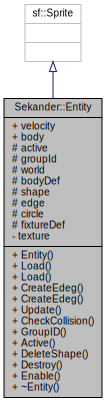
\includegraphics[width=178pt]{classSekander_1_1Entity__coll__graph}
\end{center}
\end{figure}
\subsection*{Public Member Functions}
\begin{DoxyCompactItemize}
\item 
\hyperlink{classSekander_1_1Entity_a2457570ea4a0a1009937a153f8f071f8}{Entity} (b2\+World $\ast$\hyperlink{classSekander_1_1Entity_a6c88c4e735203734409fdd7b1eddca39}{world})
\item 
void \hyperlink{classSekander_1_1Entity_a80ce51e0d09a5ac63eb3c385c47f5d73}{Load} (std\+::string filename, bool dynamic, unsigned const short int x\+\_\+frame, unsigned const short int y\+\_\+frame)
\item 
void \hyperlink{classSekander_1_1Entity_a3381ab7a718fbb980415910f47970468}{Load} (std\+::string filename, bool dynamic, struct \hyperlink{structSekander_1_1b0x__2d__SHAPES}{b0x\+\_\+2d\+\_\+\+S\+H\+A\+P\+ES} $\ast$\hyperlink{classSekander_1_1Entity_a51d32e27f0af3c9f1d68cc27117310ad}{shape}, unsigned const short int x\+\_\+frame, unsigned const short int y\+\_\+frame)
\item 
void \hyperlink{classSekander_1_1Entity_a0f2ae50422b408ef0de2cdcb31f120b4}{Create\+Edeg} (float, float, float, float)
\item 
void \hyperlink{classSekander_1_1Entity_a194f6b6f8a256a3bc0ee73f3eadeb0d0}{Create\+Edeg} ()
\item 
bool \hyperlink{classSekander_1_1Entity_a37320c3ef99e534f80f0306ebdf084ed}{Update} (sf\+::\+Render\+Window \&window)
\item 
bool \hyperlink{classSekander_1_1Entity_a202c7a8db6bcd754ebdd907d4383a6fb}{Check\+Collision} (\hyperlink{classSekander_1_1Entity}{Entity} $\ast$entity)
\item 
int \hyperlink{classSekander_1_1Entity_aaca12636d13d15fe2c84d48c64c43dc4}{Group\+ID} ()
\item 
int \hyperlink{classSekander_1_1Entity_af8b43d3ca6c6740d3e356d98656fa370}{Active} ()
\item 
void \hyperlink{classSekander_1_1Entity_a55dcbd586dfa0b339d5116ff14d58cbd}{Delete\+Shape} ()
\item 
void \hyperlink{classSekander_1_1Entity_a85095c868a53dffcb7d1f9c080448c7f}{Destroy} ()
\item 
void \hyperlink{classSekander_1_1Entity_a084a9bfb47b0efd2c5098e5f97b51c79}{Enable} ()
\item 
\hyperlink{classSekander_1_1Entity_a2246c81f180544956e614c786b7a2427}{$\sim$\+Entity} ()
\end{DoxyCompactItemize}
\subsection*{Public Attributes}
\begin{DoxyCompactItemize}
\item 
sf\+::\+Vector2f \hyperlink{classSekander_1_1Entity_a7c88f6c5a89eca36cb1204c4eaf0868e}{velocity}
\item 
b2\+Body $\ast$ \hyperlink{classSekander_1_1Entity_a61bec1a7b77dd9b5e08c0908566450d4}{body}
\end{DoxyCompactItemize}
\subsection*{Protected Attributes}
\begin{DoxyCompactItemize}
\item 
int \hyperlink{classSekander_1_1Entity_a6bd181c05edd3e27fa18efdd5dab2895}{active}
\item 
int \hyperlink{classSekander_1_1Entity_a877b3b7b7b81c7e11cb174d1a4fc3b85}{group\+Id}
\item 
b2\+World $\ast$ \hyperlink{classSekander_1_1Entity_a6c88c4e735203734409fdd7b1eddca39}{world}
\item 
b2\+Body\+Def $\ast$ \hyperlink{classSekander_1_1Entity_af8218d721852341a99eb08ee8ead53ff}{body\+Def}
\item 
b2\+Polygon\+Shape $\ast$ \hyperlink{classSekander_1_1Entity_a51d32e27f0af3c9f1d68cc27117310ad}{shape}
\item 
b2\+Edge\+Shape $\ast$ \hyperlink{classSekander_1_1Entity_a85af7309806860be286eb7b7fa89856e}{edge}
\item 
b2\+Circle\+Shape $\ast$ \hyperlink{classSekander_1_1Entity_ab1117f25502fe84887cae07b40272bbf}{circle}
\item 
b2\+Fixture\+Def $\ast$ \hyperlink{classSekander_1_1Entity_a1320e01ecadb8733a7a6204c8383bd4c}{fixture\+Def}
\end{DoxyCompactItemize}
\subsection*{Private Attributes}
\begin{DoxyCompactItemize}
\item 
sf\+::\+Texture $\ast$ \hyperlink{classSekander_1_1Entity_afb04e74d48d113702c32c991accda0cc}{texture}
\end{DoxyCompactItemize}


\subsection{Constructor \& Destructor Documentation}
\mbox{\Hypertarget{classSekander_1_1Entity_a2457570ea4a0a1009937a153f8f071f8}\label{classSekander_1_1Entity_a2457570ea4a0a1009937a153f8f071f8}} 
\index{Sekander\+::\+Entity@{Sekander\+::\+Entity}!Entity@{Entity}}
\index{Entity@{Entity}!Sekander\+::\+Entity@{Sekander\+::\+Entity}}
\subsubsection{\texorpdfstring{Entity()}{Entity()}}
{\footnotesize\ttfamily Sekander\+::\+Entity\+::\+Entity (\begin{DoxyParamCaption}\item[{b2\+World $\ast$}]{world }\end{DoxyParamCaption})}

\mbox{\Hypertarget{classSekander_1_1Entity_a2246c81f180544956e614c786b7a2427}\label{classSekander_1_1Entity_a2246c81f180544956e614c786b7a2427}} 
\index{Sekander\+::\+Entity@{Sekander\+::\+Entity}!````~Entity@{$\sim$\+Entity}}
\index{````~Entity@{$\sim$\+Entity}!Sekander\+::\+Entity@{Sekander\+::\+Entity}}
\subsubsection{\texorpdfstring{$\sim$\+Entity()}{~Entity()}}
{\footnotesize\ttfamily Sekander\+::\+Entity\+::$\sim$\+Entity (\begin{DoxyParamCaption}{ }\end{DoxyParamCaption})}



\subsection{Member Function Documentation}
\mbox{\Hypertarget{classSekander_1_1Entity_af8b43d3ca6c6740d3e356d98656fa370}\label{classSekander_1_1Entity_af8b43d3ca6c6740d3e356d98656fa370}} 
\index{Sekander\+::\+Entity@{Sekander\+::\+Entity}!Active@{Active}}
\index{Active@{Active}!Sekander\+::\+Entity@{Sekander\+::\+Entity}}
\subsubsection{\texorpdfstring{Active()}{Active()}}
{\footnotesize\ttfamily int Sekander\+::\+Entity\+::\+Active (\begin{DoxyParamCaption}{ }\end{DoxyParamCaption})\hspace{0.3cm}{\ttfamily [inline]}}

\mbox{\Hypertarget{classSekander_1_1Entity_a202c7a8db6bcd754ebdd907d4383a6fb}\label{classSekander_1_1Entity_a202c7a8db6bcd754ebdd907d4383a6fb}} 
\index{Sekander\+::\+Entity@{Sekander\+::\+Entity}!Check\+Collision@{Check\+Collision}}
\index{Check\+Collision@{Check\+Collision}!Sekander\+::\+Entity@{Sekander\+::\+Entity}}
\subsubsection{\texorpdfstring{Check\+Collision()}{CheckCollision()}}
{\footnotesize\ttfamily bool Sekander\+::\+Entity\+::\+Check\+Collision (\begin{DoxyParamCaption}\item[{\hyperlink{classSekander_1_1Entity}{Entity} $\ast$}]{entity }\end{DoxyParamCaption})}

\mbox{\Hypertarget{classSekander_1_1Entity_a0f2ae50422b408ef0de2cdcb31f120b4}\label{classSekander_1_1Entity_a0f2ae50422b408ef0de2cdcb31f120b4}} 
\index{Sekander\+::\+Entity@{Sekander\+::\+Entity}!Create\+Edeg@{Create\+Edeg}}
\index{Create\+Edeg@{Create\+Edeg}!Sekander\+::\+Entity@{Sekander\+::\+Entity}}
\subsubsection{\texorpdfstring{Create\+Edeg()}{CreateEdeg()}\hspace{0.1cm}{\footnotesize\ttfamily [1/2]}}
{\footnotesize\ttfamily void Sekander\+::\+Entity\+::\+Create\+Edeg (\begin{DoxyParamCaption}\item[{float}]{x\+\_\+point\+\_\+origin,  }\item[{float}]{y\+\_\+point\+\_\+origin,  }\item[{float}]{x\+\_\+point\+\_\+dest,  }\item[{float}]{y\+\_\+point\+\_\+dest }\end{DoxyParamCaption})}

\mbox{\Hypertarget{classSekander_1_1Entity_a194f6b6f8a256a3bc0ee73f3eadeb0d0}\label{classSekander_1_1Entity_a194f6b6f8a256a3bc0ee73f3eadeb0d0}} 
\index{Sekander\+::\+Entity@{Sekander\+::\+Entity}!Create\+Edeg@{Create\+Edeg}}
\index{Create\+Edeg@{Create\+Edeg}!Sekander\+::\+Entity@{Sekander\+::\+Entity}}
\subsubsection{\texorpdfstring{Create\+Edeg()}{CreateEdeg()}\hspace{0.1cm}{\footnotesize\ttfamily [2/2]}}
{\footnotesize\ttfamily void Sekander\+::\+Entity\+::\+Create\+Edeg (\begin{DoxyParamCaption}{ }\end{DoxyParamCaption})}

\mbox{\Hypertarget{classSekander_1_1Entity_a55dcbd586dfa0b339d5116ff14d58cbd}\label{classSekander_1_1Entity_a55dcbd586dfa0b339d5116ff14d58cbd}} 
\index{Sekander\+::\+Entity@{Sekander\+::\+Entity}!Delete\+Shape@{Delete\+Shape}}
\index{Delete\+Shape@{Delete\+Shape}!Sekander\+::\+Entity@{Sekander\+::\+Entity}}
\subsubsection{\texorpdfstring{Delete\+Shape()}{DeleteShape()}}
{\footnotesize\ttfamily void Sekander\+::\+Entity\+::\+Delete\+Shape (\begin{DoxyParamCaption}{ }\end{DoxyParamCaption})\hspace{0.3cm}{\ttfamily [inline]}}

\mbox{\Hypertarget{classSekander_1_1Entity_a85095c868a53dffcb7d1f9c080448c7f}\label{classSekander_1_1Entity_a85095c868a53dffcb7d1f9c080448c7f}} 
\index{Sekander\+::\+Entity@{Sekander\+::\+Entity}!Destroy@{Destroy}}
\index{Destroy@{Destroy}!Sekander\+::\+Entity@{Sekander\+::\+Entity}}
\subsubsection{\texorpdfstring{Destroy()}{Destroy()}}
{\footnotesize\ttfamily void Sekander\+::\+Entity\+::\+Destroy (\begin{DoxyParamCaption}{ }\end{DoxyParamCaption})}

\mbox{\Hypertarget{classSekander_1_1Entity_a084a9bfb47b0efd2c5098e5f97b51c79}\label{classSekander_1_1Entity_a084a9bfb47b0efd2c5098e5f97b51c79}} 
\index{Sekander\+::\+Entity@{Sekander\+::\+Entity}!Enable@{Enable}}
\index{Enable@{Enable}!Sekander\+::\+Entity@{Sekander\+::\+Entity}}
\subsubsection{\texorpdfstring{Enable()}{Enable()}}
{\footnotesize\ttfamily void Sekander\+::\+Entity\+::\+Enable (\begin{DoxyParamCaption}{ }\end{DoxyParamCaption})}

\mbox{\Hypertarget{classSekander_1_1Entity_aaca12636d13d15fe2c84d48c64c43dc4}\label{classSekander_1_1Entity_aaca12636d13d15fe2c84d48c64c43dc4}} 
\index{Sekander\+::\+Entity@{Sekander\+::\+Entity}!Group\+ID@{Group\+ID}}
\index{Group\+ID@{Group\+ID}!Sekander\+::\+Entity@{Sekander\+::\+Entity}}
\subsubsection{\texorpdfstring{Group\+I\+D()}{GroupID()}}
{\footnotesize\ttfamily int Sekander\+::\+Entity\+::\+Group\+ID (\begin{DoxyParamCaption}{ }\end{DoxyParamCaption})\hspace{0.3cm}{\ttfamily [inline]}}

\mbox{\Hypertarget{classSekander_1_1Entity_a80ce51e0d09a5ac63eb3c385c47f5d73}\label{classSekander_1_1Entity_a80ce51e0d09a5ac63eb3c385c47f5d73}} 
\index{Sekander\+::\+Entity@{Sekander\+::\+Entity}!Load@{Load}}
\index{Load@{Load}!Sekander\+::\+Entity@{Sekander\+::\+Entity}}
\subsubsection{\texorpdfstring{Load()}{Load()}\hspace{0.1cm}{\footnotesize\ttfamily [1/2]}}
{\footnotesize\ttfamily void Sekander\+::\+Entity\+::\+Load (\begin{DoxyParamCaption}\item[{std\+::string}]{filename,  }\item[{bool}]{dynamic,  }\item[{unsigned const short int}]{x\+\_\+frame,  }\item[{unsigned const short int}]{y\+\_\+frame }\end{DoxyParamCaption})}

\mbox{\Hypertarget{classSekander_1_1Entity_a3381ab7a718fbb980415910f47970468}\label{classSekander_1_1Entity_a3381ab7a718fbb980415910f47970468}} 
\index{Sekander\+::\+Entity@{Sekander\+::\+Entity}!Load@{Load}}
\index{Load@{Load}!Sekander\+::\+Entity@{Sekander\+::\+Entity}}
\subsubsection{\texorpdfstring{Load()}{Load()}\hspace{0.1cm}{\footnotesize\ttfamily [2/2]}}
{\footnotesize\ttfamily void Sekander\+::\+Entity\+::\+Load (\begin{DoxyParamCaption}\item[{std\+::string}]{filename,  }\item[{bool}]{dynamic,  }\item[{struct \hyperlink{structSekander_1_1b0x__2d__SHAPES}{b0x\+\_\+2d\+\_\+\+S\+H\+A\+P\+ES} $\ast$}]{shape,  }\item[{unsigned const short int}]{x\+\_\+frame,  }\item[{unsigned const short int}]{y\+\_\+frame }\end{DoxyParamCaption})}

\mbox{\Hypertarget{classSekander_1_1Entity_a37320c3ef99e534f80f0306ebdf084ed}\label{classSekander_1_1Entity_a37320c3ef99e534f80f0306ebdf084ed}} 
\index{Sekander\+::\+Entity@{Sekander\+::\+Entity}!Update@{Update}}
\index{Update@{Update}!Sekander\+::\+Entity@{Sekander\+::\+Entity}}
\subsubsection{\texorpdfstring{Update()}{Update()}}
{\footnotesize\ttfamily bool Sekander\+::\+Entity\+::\+Update (\begin{DoxyParamCaption}\item[{sf\+::\+Render\+Window \&}]{window }\end{DoxyParamCaption})}



\subsection{Member Data Documentation}
\mbox{\Hypertarget{classSekander_1_1Entity_a6bd181c05edd3e27fa18efdd5dab2895}\label{classSekander_1_1Entity_a6bd181c05edd3e27fa18efdd5dab2895}} 
\index{Sekander\+::\+Entity@{Sekander\+::\+Entity}!active@{active}}
\index{active@{active}!Sekander\+::\+Entity@{Sekander\+::\+Entity}}
\subsubsection{\texorpdfstring{active}{active}}
{\footnotesize\ttfamily int Sekander\+::\+Entity\+::active\hspace{0.3cm}{\ttfamily [protected]}}

\mbox{\Hypertarget{classSekander_1_1Entity_a61bec1a7b77dd9b5e08c0908566450d4}\label{classSekander_1_1Entity_a61bec1a7b77dd9b5e08c0908566450d4}} 
\index{Sekander\+::\+Entity@{Sekander\+::\+Entity}!body@{body}}
\index{body@{body}!Sekander\+::\+Entity@{Sekander\+::\+Entity}}
\subsubsection{\texorpdfstring{body}{body}}
{\footnotesize\ttfamily b2\+Body$\ast$ Sekander\+::\+Entity\+::body}

\mbox{\Hypertarget{classSekander_1_1Entity_af8218d721852341a99eb08ee8ead53ff}\label{classSekander_1_1Entity_af8218d721852341a99eb08ee8ead53ff}} 
\index{Sekander\+::\+Entity@{Sekander\+::\+Entity}!body\+Def@{body\+Def}}
\index{body\+Def@{body\+Def}!Sekander\+::\+Entity@{Sekander\+::\+Entity}}
\subsubsection{\texorpdfstring{body\+Def}{bodyDef}}
{\footnotesize\ttfamily b2\+Body\+Def$\ast$ Sekander\+::\+Entity\+::body\+Def\hspace{0.3cm}{\ttfamily [protected]}}

\mbox{\Hypertarget{classSekander_1_1Entity_ab1117f25502fe84887cae07b40272bbf}\label{classSekander_1_1Entity_ab1117f25502fe84887cae07b40272bbf}} 
\index{Sekander\+::\+Entity@{Sekander\+::\+Entity}!circle@{circle}}
\index{circle@{circle}!Sekander\+::\+Entity@{Sekander\+::\+Entity}}
\subsubsection{\texorpdfstring{circle}{circle}}
{\footnotesize\ttfamily b2\+Circle\+Shape$\ast$ Sekander\+::\+Entity\+::circle\hspace{0.3cm}{\ttfamily [protected]}}

\mbox{\Hypertarget{classSekander_1_1Entity_a85af7309806860be286eb7b7fa89856e}\label{classSekander_1_1Entity_a85af7309806860be286eb7b7fa89856e}} 
\index{Sekander\+::\+Entity@{Sekander\+::\+Entity}!edge@{edge}}
\index{edge@{edge}!Sekander\+::\+Entity@{Sekander\+::\+Entity}}
\subsubsection{\texorpdfstring{edge}{edge}}
{\footnotesize\ttfamily b2\+Edge\+Shape$\ast$ Sekander\+::\+Entity\+::edge\hspace{0.3cm}{\ttfamily [protected]}}

\mbox{\Hypertarget{classSekander_1_1Entity_a1320e01ecadb8733a7a6204c8383bd4c}\label{classSekander_1_1Entity_a1320e01ecadb8733a7a6204c8383bd4c}} 
\index{Sekander\+::\+Entity@{Sekander\+::\+Entity}!fixture\+Def@{fixture\+Def}}
\index{fixture\+Def@{fixture\+Def}!Sekander\+::\+Entity@{Sekander\+::\+Entity}}
\subsubsection{\texorpdfstring{fixture\+Def}{fixtureDef}}
{\footnotesize\ttfamily b2\+Fixture\+Def$\ast$ Sekander\+::\+Entity\+::fixture\+Def\hspace{0.3cm}{\ttfamily [protected]}}

\mbox{\Hypertarget{classSekander_1_1Entity_a877b3b7b7b81c7e11cb174d1a4fc3b85}\label{classSekander_1_1Entity_a877b3b7b7b81c7e11cb174d1a4fc3b85}} 
\index{Sekander\+::\+Entity@{Sekander\+::\+Entity}!group\+Id@{group\+Id}}
\index{group\+Id@{group\+Id}!Sekander\+::\+Entity@{Sekander\+::\+Entity}}
\subsubsection{\texorpdfstring{group\+Id}{groupId}}
{\footnotesize\ttfamily int Sekander\+::\+Entity\+::group\+Id\hspace{0.3cm}{\ttfamily [protected]}}

\mbox{\Hypertarget{classSekander_1_1Entity_a51d32e27f0af3c9f1d68cc27117310ad}\label{classSekander_1_1Entity_a51d32e27f0af3c9f1d68cc27117310ad}} 
\index{Sekander\+::\+Entity@{Sekander\+::\+Entity}!shape@{shape}}
\index{shape@{shape}!Sekander\+::\+Entity@{Sekander\+::\+Entity}}
\subsubsection{\texorpdfstring{shape}{shape}}
{\footnotesize\ttfamily b2\+Polygon\+Shape$\ast$ Sekander\+::\+Entity\+::shape\hspace{0.3cm}{\ttfamily [protected]}}

\mbox{\Hypertarget{classSekander_1_1Entity_afb04e74d48d113702c32c991accda0cc}\label{classSekander_1_1Entity_afb04e74d48d113702c32c991accda0cc}} 
\index{Sekander\+::\+Entity@{Sekander\+::\+Entity}!texture@{texture}}
\index{texture@{texture}!Sekander\+::\+Entity@{Sekander\+::\+Entity}}
\subsubsection{\texorpdfstring{texture}{texture}}
{\footnotesize\ttfamily sf\+::\+Texture$\ast$ Sekander\+::\+Entity\+::texture\hspace{0.3cm}{\ttfamily [private]}}

\mbox{\Hypertarget{classSekander_1_1Entity_a7c88f6c5a89eca36cb1204c4eaf0868e}\label{classSekander_1_1Entity_a7c88f6c5a89eca36cb1204c4eaf0868e}} 
\index{Sekander\+::\+Entity@{Sekander\+::\+Entity}!velocity@{velocity}}
\index{velocity@{velocity}!Sekander\+::\+Entity@{Sekander\+::\+Entity}}
\subsubsection{\texorpdfstring{velocity}{velocity}}
{\footnotesize\ttfamily sf\+::\+Vector2f Sekander\+::\+Entity\+::velocity}

\mbox{\Hypertarget{classSekander_1_1Entity_a6c88c4e735203734409fdd7b1eddca39}\label{classSekander_1_1Entity_a6c88c4e735203734409fdd7b1eddca39}} 
\index{Sekander\+::\+Entity@{Sekander\+::\+Entity}!world@{world}}
\index{world@{world}!Sekander\+::\+Entity@{Sekander\+::\+Entity}}
\subsubsection{\texorpdfstring{world}{world}}
{\footnotesize\ttfamily b2\+World$\ast$ Sekander\+::\+Entity\+::world\hspace{0.3cm}{\ttfamily [protected]}}



The documentation for this class was generated from the following files\+:\begin{DoxyCompactItemize}
\item 
/mnt/hdd/\+C0de/\+Engines/\+S\+F\+M\+L/\+S\+F\+M\+L\+\_\+\+Engine/include/\hyperlink{entity_8h}{entity.\+h}\item 
/mnt/hdd/\+C0de/\+Engines/\+S\+F\+M\+L/\+S\+F\+M\+L\+\_\+\+Engine/src/\hyperlink{entity_8cpp}{entity.\+cpp}\end{DoxyCompactItemize}

\hypertarget{classSekander_1_1EntityManager}{}\section{Sekander\+:\+:Entity\+Manager Class Reference}
\label{classSekander_1_1EntityManager}\index{Sekander\+::\+Entity\+Manager@{Sekander\+::\+Entity\+Manager}}


{\ttfamily \#include $<$entity\+\_\+manager.\+h$>$}



Collaboration diagram for Sekander\+:\+:Entity\+Manager\+:
\nopagebreak
\begin{figure}[H]
\begin{center}
\leavevmode
\includegraphics[width=207pt]{classSekander_1_1EntityManager__coll__graph}
\end{center}
\end{figure}
\subsection*{Public Member Functions}
\begin{DoxyCompactItemize}
\item 
\hyperlink{classSekander_1_1EntityManager_a98a085b51de53396a9a9b7803422c6ff}{Entity\+Manager} ()
\item 
void \hyperlink{classSekander_1_1EntityManager_afaae67bb65ba3dac38417caf4e2c2f2b}{Add} (std\+::string name, std\+::string filename, bool dynamic, unsigned const short int, unsigned const short int)
\item 
void \hyperlink{classSekander_1_1EntityManager_a4b0fdd5fb634533e04fe33c48a25f6e9}{Add} (std\+::string name, std\+::string filename, bool dynamic, \hyperlink{namespaceSekander_aed8eb219f4685b29738464e9f32c5d94}{shape\+\_\+options})
\item 
void \hyperlink{classSekander_1_1EntityManager_ab5c80c9646fea25cb0ab110a4ac51d38}{new\+Edge} (std\+::string name)
\item 
void \hyperlink{classSekander_1_1EntityManager_a0debb38e1fb1e88d3d4e5af522e80b90}{new\+Edge} (std\+::string, float, float, float, float)
\item 
\hyperlink{classSekander_1_1Entity}{Entity} $\ast$ \hyperlink{classSekander_1_1EntityManager_a9c4fa2dc9649cdd63ba64bea469c267c}{Get} (std\+::string name)
\item 
void \hyperlink{classSekander_1_1EntityManager_a10a4ff59b03ab00e9688063de4bc9c98}{List\+All\+Enties} ()
\item 
std\+::unordered\+\_\+map$<$ std\+::string, \hyperlink{classSekander_1_1Entity}{Entity} $\ast$ $>$ \hyperlink{classSekander_1_1EntityManager_aff93fbae10b873e3bd402ad1acc23b32}{Return\+Map} ()
\item 
bool \hyperlink{classSekander_1_1EntityManager_ac2385e541fe3ac866f90daad53892a00}{Update} (sf\+::\+Render\+Window \&window)
\item 
void \hyperlink{classSekander_1_1EntityManager_a24bc2a30b608d425aaeded98c1c18cfc}{Render} (sf\+::\+Render\+Window \&window)
\item 
void \hyperlink{classSekander_1_1EntityManager_a71d1b6d1c1a80efa0117e3bf8e982562}{Delete\+Entity} ()
\item 
void \hyperlink{classSekander_1_1EntityManager_a5ce5af4eb68c0dd7d019877f65ea4c83}{Enable\+Entity} ()
\item 
\hyperlink{classSekander_1_1EntityManager_adcd3f85835de9ac2eb2af3c876899244}{$\sim$\+Entity\+Manager} ()
\end{DoxyCompactItemize}
\subsection*{Private Attributes}
\begin{DoxyCompactItemize}
\item 
std\+::unordered\+\_\+map$<$ std\+::string, \hyperlink{classSekander_1_1Entity}{Entity} $\ast$ $>$ \hyperlink{classSekander_1_1EntityManager_a8ee9d64c41a23790dc4c1e3f1ce3ea56}{entities}
\item 
b2\+World $\ast$ \hyperlink{classSekander_1_1EntityManager_ad2d38ab329ff4b57b2d66b807dacdbb3}{world}
\item 
sf\+::\+Vertex \hyperlink{classSekander_1_1EntityManager_af00445583df085f6c28390b4b940ccc5}{vertices} \mbox{[}2\mbox{]}
\item 
std\+::vector$<$ sf\+::\+Vertex $>$ \hyperlink{classSekander_1_1EntityManager_a40f45e16f17a739a730c1373021e5cc9}{vertices\+\_\+vec}
\end{DoxyCompactItemize}


\subsection{Constructor \& Destructor Documentation}
\mbox{\Hypertarget{classSekander_1_1EntityManager_a98a085b51de53396a9a9b7803422c6ff}\label{classSekander_1_1EntityManager_a98a085b51de53396a9a9b7803422c6ff}} 
\index{Sekander\+::\+Entity\+Manager@{Sekander\+::\+Entity\+Manager}!Entity\+Manager@{Entity\+Manager}}
\index{Entity\+Manager@{Entity\+Manager}!Sekander\+::\+Entity\+Manager@{Sekander\+::\+Entity\+Manager}}
\subsubsection{\texorpdfstring{Entity\+Manager()}{EntityManager()}}
{\footnotesize\ttfamily Sekander\+::\+Entity\+Manager\+::\+Entity\+Manager (\begin{DoxyParamCaption}{ }\end{DoxyParamCaption})}

\mbox{\Hypertarget{classSekander_1_1EntityManager_adcd3f85835de9ac2eb2af3c876899244}\label{classSekander_1_1EntityManager_adcd3f85835de9ac2eb2af3c876899244}} 
\index{Sekander\+::\+Entity\+Manager@{Sekander\+::\+Entity\+Manager}!````~Entity\+Manager@{$\sim$\+Entity\+Manager}}
\index{````~Entity\+Manager@{$\sim$\+Entity\+Manager}!Sekander\+::\+Entity\+Manager@{Sekander\+::\+Entity\+Manager}}
\subsubsection{\texorpdfstring{$\sim$\+Entity\+Manager()}{~EntityManager()}}
{\footnotesize\ttfamily Sekander\+::\+Entity\+Manager\+::$\sim$\+Entity\+Manager (\begin{DoxyParamCaption}{ }\end{DoxyParamCaption})}



\subsection{Member Function Documentation}
\mbox{\Hypertarget{classSekander_1_1EntityManager_afaae67bb65ba3dac38417caf4e2c2f2b}\label{classSekander_1_1EntityManager_afaae67bb65ba3dac38417caf4e2c2f2b}} 
\index{Sekander\+::\+Entity\+Manager@{Sekander\+::\+Entity\+Manager}!Add@{Add}}
\index{Add@{Add}!Sekander\+::\+Entity\+Manager@{Sekander\+::\+Entity\+Manager}}
\subsubsection{\texorpdfstring{Add()}{Add()}\hspace{0.1cm}{\footnotesize\ttfamily [1/2]}}
{\footnotesize\ttfamily void Sekander\+::\+Entity\+Manager\+::\+Add (\begin{DoxyParamCaption}\item[{std\+::string}]{name,  }\item[{std\+::string}]{filename,  }\item[{bool}]{dynamic,  }\item[{unsigned const short int}]{x\+\_\+frames,  }\item[{unsigned const short int}]{y\+\_\+frames }\end{DoxyParamCaption})}

\mbox{\Hypertarget{classSekander_1_1EntityManager_a4b0fdd5fb634533e04fe33c48a25f6e9}\label{classSekander_1_1EntityManager_a4b0fdd5fb634533e04fe33c48a25f6e9}} 
\index{Sekander\+::\+Entity\+Manager@{Sekander\+::\+Entity\+Manager}!Add@{Add}}
\index{Add@{Add}!Sekander\+::\+Entity\+Manager@{Sekander\+::\+Entity\+Manager}}
\subsubsection{\texorpdfstring{Add()}{Add()}\hspace{0.1cm}{\footnotesize\ttfamily [2/2]}}
{\footnotesize\ttfamily void Sekander\+::\+Entity\+Manager\+::\+Add (\begin{DoxyParamCaption}\item[{std\+::string}]{name,  }\item[{std\+::string}]{filename,  }\item[{bool}]{dynamic,  }\item[{\hyperlink{namespaceSekander_aed8eb219f4685b29738464e9f32c5d94}{shape\+\_\+options}}]{shapes }\end{DoxyParamCaption})}

\mbox{\Hypertarget{classSekander_1_1EntityManager_a71d1b6d1c1a80efa0117e3bf8e982562}\label{classSekander_1_1EntityManager_a71d1b6d1c1a80efa0117e3bf8e982562}} 
\index{Sekander\+::\+Entity\+Manager@{Sekander\+::\+Entity\+Manager}!Delete\+Entity@{Delete\+Entity}}
\index{Delete\+Entity@{Delete\+Entity}!Sekander\+::\+Entity\+Manager@{Sekander\+::\+Entity\+Manager}}
\subsubsection{\texorpdfstring{Delete\+Entity()}{DeleteEntity()}}
{\footnotesize\ttfamily void Sekander\+::\+Entity\+Manager\+::\+Delete\+Entity (\begin{DoxyParamCaption}{ }\end{DoxyParamCaption})}

\mbox{\Hypertarget{classSekander_1_1EntityManager_a5ce5af4eb68c0dd7d019877f65ea4c83}\label{classSekander_1_1EntityManager_a5ce5af4eb68c0dd7d019877f65ea4c83}} 
\index{Sekander\+::\+Entity\+Manager@{Sekander\+::\+Entity\+Manager}!Enable\+Entity@{Enable\+Entity}}
\index{Enable\+Entity@{Enable\+Entity}!Sekander\+::\+Entity\+Manager@{Sekander\+::\+Entity\+Manager}}
\subsubsection{\texorpdfstring{Enable\+Entity()}{EnableEntity()}}
{\footnotesize\ttfamily void Sekander\+::\+Entity\+Manager\+::\+Enable\+Entity (\begin{DoxyParamCaption}{ }\end{DoxyParamCaption})}

\mbox{\Hypertarget{classSekander_1_1EntityManager_a9c4fa2dc9649cdd63ba64bea469c267c}\label{classSekander_1_1EntityManager_a9c4fa2dc9649cdd63ba64bea469c267c}} 
\index{Sekander\+::\+Entity\+Manager@{Sekander\+::\+Entity\+Manager}!Get@{Get}}
\index{Get@{Get}!Sekander\+::\+Entity\+Manager@{Sekander\+::\+Entity\+Manager}}
\subsubsection{\texorpdfstring{Get()}{Get()}}
{\footnotesize\ttfamily \hyperlink{classSekander_1_1Entity}{Entity} $\ast$ Sekander\+::\+Entity\+Manager\+::\+Get (\begin{DoxyParamCaption}\item[{std\+::string}]{name }\end{DoxyParamCaption})}

\mbox{\Hypertarget{classSekander_1_1EntityManager_a10a4ff59b03ab00e9688063de4bc9c98}\label{classSekander_1_1EntityManager_a10a4ff59b03ab00e9688063de4bc9c98}} 
\index{Sekander\+::\+Entity\+Manager@{Sekander\+::\+Entity\+Manager}!List\+All\+Enties@{List\+All\+Enties}}
\index{List\+All\+Enties@{List\+All\+Enties}!Sekander\+::\+Entity\+Manager@{Sekander\+::\+Entity\+Manager}}
\subsubsection{\texorpdfstring{List\+All\+Enties()}{ListAllEnties()}}
{\footnotesize\ttfamily void Sekander\+::\+Entity\+Manager\+::\+List\+All\+Enties (\begin{DoxyParamCaption}{ }\end{DoxyParamCaption})}

\mbox{\Hypertarget{classSekander_1_1EntityManager_ab5c80c9646fea25cb0ab110a4ac51d38}\label{classSekander_1_1EntityManager_ab5c80c9646fea25cb0ab110a4ac51d38}} 
\index{Sekander\+::\+Entity\+Manager@{Sekander\+::\+Entity\+Manager}!new\+Edge@{new\+Edge}}
\index{new\+Edge@{new\+Edge}!Sekander\+::\+Entity\+Manager@{Sekander\+::\+Entity\+Manager}}
\subsubsection{\texorpdfstring{new\+Edge()}{newEdge()}\hspace{0.1cm}{\footnotesize\ttfamily [1/2]}}
{\footnotesize\ttfamily void Sekander\+::\+Entity\+Manager\+::new\+Edge (\begin{DoxyParamCaption}\item[{std\+::string}]{name }\end{DoxyParamCaption})}

\mbox{\Hypertarget{classSekander_1_1EntityManager_a0debb38e1fb1e88d3d4e5af522e80b90}\label{classSekander_1_1EntityManager_a0debb38e1fb1e88d3d4e5af522e80b90}} 
\index{Sekander\+::\+Entity\+Manager@{Sekander\+::\+Entity\+Manager}!new\+Edge@{new\+Edge}}
\index{new\+Edge@{new\+Edge}!Sekander\+::\+Entity\+Manager@{Sekander\+::\+Entity\+Manager}}
\subsubsection{\texorpdfstring{new\+Edge()}{newEdge()}\hspace{0.1cm}{\footnotesize\ttfamily [2/2]}}
{\footnotesize\ttfamily void Sekander\+::\+Entity\+Manager\+::new\+Edge (\begin{DoxyParamCaption}\item[{std\+::string}]{name,  }\item[{float}]{xo,  }\item[{float}]{yo,  }\item[{float}]{xd,  }\item[{float}]{yd }\end{DoxyParamCaption})}

\mbox{\Hypertarget{classSekander_1_1EntityManager_a24bc2a30b608d425aaeded98c1c18cfc}\label{classSekander_1_1EntityManager_a24bc2a30b608d425aaeded98c1c18cfc}} 
\index{Sekander\+::\+Entity\+Manager@{Sekander\+::\+Entity\+Manager}!Render@{Render}}
\index{Render@{Render}!Sekander\+::\+Entity\+Manager@{Sekander\+::\+Entity\+Manager}}
\subsubsection{\texorpdfstring{Render()}{Render()}}
{\footnotesize\ttfamily void Sekander\+::\+Entity\+Manager\+::\+Render (\begin{DoxyParamCaption}\item[{sf\+::\+Render\+Window \&}]{window }\end{DoxyParamCaption})}

\mbox{\Hypertarget{classSekander_1_1EntityManager_aff93fbae10b873e3bd402ad1acc23b32}\label{classSekander_1_1EntityManager_aff93fbae10b873e3bd402ad1acc23b32}} 
\index{Sekander\+::\+Entity\+Manager@{Sekander\+::\+Entity\+Manager}!Return\+Map@{Return\+Map}}
\index{Return\+Map@{Return\+Map}!Sekander\+::\+Entity\+Manager@{Sekander\+::\+Entity\+Manager}}
\subsubsection{\texorpdfstring{Return\+Map()}{ReturnMap()}}
{\footnotesize\ttfamily std\+::unordered\+\_\+map$<$std\+::string, \hyperlink{classSekander_1_1Entity}{Entity}$\ast$$>$ Sekander\+::\+Entity\+Manager\+::\+Return\+Map (\begin{DoxyParamCaption}{ }\end{DoxyParamCaption})\hspace{0.3cm}{\ttfamily [inline]}}

\mbox{\Hypertarget{classSekander_1_1EntityManager_ac2385e541fe3ac866f90daad53892a00}\label{classSekander_1_1EntityManager_ac2385e541fe3ac866f90daad53892a00}} 
\index{Sekander\+::\+Entity\+Manager@{Sekander\+::\+Entity\+Manager}!Update@{Update}}
\index{Update@{Update}!Sekander\+::\+Entity\+Manager@{Sekander\+::\+Entity\+Manager}}
\subsubsection{\texorpdfstring{Update()}{Update()}}
{\footnotesize\ttfamily bool Sekander\+::\+Entity\+Manager\+::\+Update (\begin{DoxyParamCaption}\item[{sf\+::\+Render\+Window \&}]{window }\end{DoxyParamCaption})}



\subsection{Member Data Documentation}
\mbox{\Hypertarget{classSekander_1_1EntityManager_a8ee9d64c41a23790dc4c1e3f1ce3ea56}\label{classSekander_1_1EntityManager_a8ee9d64c41a23790dc4c1e3f1ce3ea56}} 
\index{Sekander\+::\+Entity\+Manager@{Sekander\+::\+Entity\+Manager}!entities@{entities}}
\index{entities@{entities}!Sekander\+::\+Entity\+Manager@{Sekander\+::\+Entity\+Manager}}
\subsubsection{\texorpdfstring{entities}{entities}}
{\footnotesize\ttfamily std\+::unordered\+\_\+map$<$std\+::string, \hyperlink{classSekander_1_1Entity}{Entity}$\ast$$>$ Sekander\+::\+Entity\+Manager\+::entities\hspace{0.3cm}{\ttfamily [private]}}

\mbox{\Hypertarget{classSekander_1_1EntityManager_af00445583df085f6c28390b4b940ccc5}\label{classSekander_1_1EntityManager_af00445583df085f6c28390b4b940ccc5}} 
\index{Sekander\+::\+Entity\+Manager@{Sekander\+::\+Entity\+Manager}!vertices@{vertices}}
\index{vertices@{vertices}!Sekander\+::\+Entity\+Manager@{Sekander\+::\+Entity\+Manager}}
\subsubsection{\texorpdfstring{vertices}{vertices}}
{\footnotesize\ttfamily sf\+::\+Vertex Sekander\+::\+Entity\+Manager\+::vertices\mbox{[}2\mbox{]}\hspace{0.3cm}{\ttfamily [private]}}

\mbox{\Hypertarget{classSekander_1_1EntityManager_a40f45e16f17a739a730c1373021e5cc9}\label{classSekander_1_1EntityManager_a40f45e16f17a739a730c1373021e5cc9}} 
\index{Sekander\+::\+Entity\+Manager@{Sekander\+::\+Entity\+Manager}!vertices\+\_\+vec@{vertices\+\_\+vec}}
\index{vertices\+\_\+vec@{vertices\+\_\+vec}!Sekander\+::\+Entity\+Manager@{Sekander\+::\+Entity\+Manager}}
\subsubsection{\texorpdfstring{vertices\+\_\+vec}{vertices\_vec}}
{\footnotesize\ttfamily std\+::vector$<$sf\+::\+Vertex$>$ Sekander\+::\+Entity\+Manager\+::vertices\+\_\+vec\hspace{0.3cm}{\ttfamily [private]}}

\mbox{\Hypertarget{classSekander_1_1EntityManager_ad2d38ab329ff4b57b2d66b807dacdbb3}\label{classSekander_1_1EntityManager_ad2d38ab329ff4b57b2d66b807dacdbb3}} 
\index{Sekander\+::\+Entity\+Manager@{Sekander\+::\+Entity\+Manager}!world@{world}}
\index{world@{world}!Sekander\+::\+Entity\+Manager@{Sekander\+::\+Entity\+Manager}}
\subsubsection{\texorpdfstring{world}{world}}
{\footnotesize\ttfamily b2\+World$\ast$ Sekander\+::\+Entity\+Manager\+::world\hspace{0.3cm}{\ttfamily [private]}}



The documentation for this class was generated from the following files\+:\begin{DoxyCompactItemize}
\item 
/mnt/hdd/\+C0de/\+Engines/\+S\+F\+M\+L/\+S\+F\+M\+L\+\_\+\+Engine/include/\hyperlink{entity__manager_8h}{entity\+\_\+manager.\+h}\item 
/mnt/hdd/\+C0de/\+Engines/\+S\+F\+M\+L/\+S\+F\+M\+L\+\_\+\+Engine/src/\hyperlink{entity__manager_8cpp}{entity\+\_\+manager.\+cpp}\end{DoxyCompactItemize}

\hypertarget{classSekander_1_1Game}{}\section{Sekander\+:\+:Game Class Reference}
\label{classSekander_1_1Game}\index{Sekander\+::\+Game@{Sekander\+::\+Game}}


{\ttfamily \#include $<$Game.\+hpp$>$}



Collaboration diagram for Sekander\+:\+:Game\+:
\nopagebreak
\begin{figure}[H]
\begin{center}
\leavevmode
\includegraphics[width=186pt]{classSekander_1_1Game__coll__graph}
\end{center}
\end{figure}
\subsection*{Public Member Functions}
\begin{DoxyCompactItemize}
\item 
\hyperlink{classSekander_1_1Game_a53c182b8b8b63723740aaef1b0cc25a0}{Game} (int width, int height, std\+::string title)
\item 
\hyperlink{classSekander_1_1Game_afe9c8ee4d47148de8fed696efe7bd9ac}{Game} (int width, int height, std\+::string title, bool)
\item 
\hyperlink{classSekander_1_1Game_a187c141c1b8b70416dccfbfb15d2a3db}{Game} (int width, int height, std\+::string title, bool, const char $\ast$xml\+\_\+\+D\+OC)
\item 
void \hyperlink{classSekander_1_1Game_a2bf4207f57e28e619fcdf383079c3a9d}{Toggle\+Fullscreen} ()
\item 
bool \hyperlink{classSekander_1_1Game_a70fe3c4cc2af6708dc19ffd54a782283}{Is\+Done} ()
\item 
bool \hyperlink{classSekander_1_1Game_aa919e9a5695d21c1ab19b2c8abe54041}{Is\+Fullscreen} ()
\end{DoxyCompactItemize}
\subsection*{Private Member Functions}
\begin{DoxyCompactItemize}
\item 
void \hyperlink{classSekander_1_1Game_ac944cfcfb5783b7788e591cd748ee51e}{Run} ()
\end{DoxyCompactItemize}
\subsection*{Private Attributes}
\begin{DoxyCompactItemize}
\item 
const float \hyperlink{classSekander_1_1Game_ad38a233b0015262e84bd4f200378c295}{dt} = 1.\+0f / 60.\+0f
\item 
sf\+::\+Clock \hyperlink{classSekander_1_1Game_a834d5264e03e48eb2cf4fbc11e46b58d}{\+\_\+clock}
\item 
\hyperlink{namespaceSekander_a1d69b002ba2d23020901c28f0def5e16}{Game\+Data\+Ref} \hyperlink{classSekander_1_1Game_a2a48d9df37ee8bb23b687a7f9c83a471}{\+\_\+data} = std\+::make\+\_\+shared$<$\hyperlink{structSekander_1_1GameData}{Game\+Data}$>$()
\item 
bool \hyperlink{classSekander_1_1Game_a416e310b39c99a719a9429b8366e7a0b}{m\+\_\+is\+Fullscreen}
\end{DoxyCompactItemize}


\subsection{Constructor \& Destructor Documentation}
\mbox{\Hypertarget{classSekander_1_1Game_a53c182b8b8b63723740aaef1b0cc25a0}\label{classSekander_1_1Game_a53c182b8b8b63723740aaef1b0cc25a0}} 
\index{Sekander\+::\+Game@{Sekander\+::\+Game}!Game@{Game}}
\index{Game@{Game}!Sekander\+::\+Game@{Sekander\+::\+Game}}
\subsubsection{\texorpdfstring{Game()}{Game()}\hspace{0.1cm}{\footnotesize\ttfamily [1/3]}}
{\footnotesize\ttfamily Sekander\+::\+Game\+::\+Game (\begin{DoxyParamCaption}\item[{int}]{width,  }\item[{int}]{height,  }\item[{std\+::string}]{title }\end{DoxyParamCaption})}

\mbox{\Hypertarget{classSekander_1_1Game_afe9c8ee4d47148de8fed696efe7bd9ac}\label{classSekander_1_1Game_afe9c8ee4d47148de8fed696efe7bd9ac}} 
\index{Sekander\+::\+Game@{Sekander\+::\+Game}!Game@{Game}}
\index{Game@{Game}!Sekander\+::\+Game@{Sekander\+::\+Game}}
\subsubsection{\texorpdfstring{Game()}{Game()}\hspace{0.1cm}{\footnotesize\ttfamily [2/3]}}
{\footnotesize\ttfamily Sekander\+::\+Game\+::\+Game (\begin{DoxyParamCaption}\item[{int}]{width,  }\item[{int}]{height,  }\item[{std\+::string}]{title,  }\item[{bool}]{full\+Screen }\end{DoxyParamCaption})}

\mbox{\Hypertarget{classSekander_1_1Game_a187c141c1b8b70416dccfbfb15d2a3db}\label{classSekander_1_1Game_a187c141c1b8b70416dccfbfb15d2a3db}} 
\index{Sekander\+::\+Game@{Sekander\+::\+Game}!Game@{Game}}
\index{Game@{Game}!Sekander\+::\+Game@{Sekander\+::\+Game}}
\subsubsection{\texorpdfstring{Game()}{Game()}\hspace{0.1cm}{\footnotesize\ttfamily [3/3]}}
{\footnotesize\ttfamily Sekander\+::\+Game\+::\+Game (\begin{DoxyParamCaption}\item[{int}]{width,  }\item[{int}]{height,  }\item[{std\+::string}]{title,  }\item[{bool}]{full\+Screen,  }\item[{const char $\ast$}]{xml\+\_\+\+D\+OC }\end{DoxyParamCaption})}



\subsection{Member Function Documentation}
\mbox{\Hypertarget{classSekander_1_1Game_a70fe3c4cc2af6708dc19ffd54a782283}\label{classSekander_1_1Game_a70fe3c4cc2af6708dc19ffd54a782283}} 
\index{Sekander\+::\+Game@{Sekander\+::\+Game}!Is\+Done@{Is\+Done}}
\index{Is\+Done@{Is\+Done}!Sekander\+::\+Game@{Sekander\+::\+Game}}
\subsubsection{\texorpdfstring{Is\+Done()}{IsDone()}}
{\footnotesize\ttfamily bool Sekander\+::\+Game\+::\+Is\+Done (\begin{DoxyParamCaption}{ }\end{DoxyParamCaption})}

\mbox{\Hypertarget{classSekander_1_1Game_aa919e9a5695d21c1ab19b2c8abe54041}\label{classSekander_1_1Game_aa919e9a5695d21c1ab19b2c8abe54041}} 
\index{Sekander\+::\+Game@{Sekander\+::\+Game}!Is\+Fullscreen@{Is\+Fullscreen}}
\index{Is\+Fullscreen@{Is\+Fullscreen}!Sekander\+::\+Game@{Sekander\+::\+Game}}
\subsubsection{\texorpdfstring{Is\+Fullscreen()}{IsFullscreen()}}
{\footnotesize\ttfamily bool Sekander\+::\+Game\+::\+Is\+Fullscreen (\begin{DoxyParamCaption}{ }\end{DoxyParamCaption})}

\mbox{\Hypertarget{classSekander_1_1Game_ac944cfcfb5783b7788e591cd748ee51e}\label{classSekander_1_1Game_ac944cfcfb5783b7788e591cd748ee51e}} 
\index{Sekander\+::\+Game@{Sekander\+::\+Game}!Run@{Run}}
\index{Run@{Run}!Sekander\+::\+Game@{Sekander\+::\+Game}}
\subsubsection{\texorpdfstring{Run()}{Run()}}
{\footnotesize\ttfamily void Sekander\+::\+Game\+::\+Run (\begin{DoxyParamCaption}{ }\end{DoxyParamCaption})\hspace{0.3cm}{\ttfamily [private]}}

\mbox{\Hypertarget{classSekander_1_1Game_a2bf4207f57e28e619fcdf383079c3a9d}\label{classSekander_1_1Game_a2bf4207f57e28e619fcdf383079c3a9d}} 
\index{Sekander\+::\+Game@{Sekander\+::\+Game}!Toggle\+Fullscreen@{Toggle\+Fullscreen}}
\index{Toggle\+Fullscreen@{Toggle\+Fullscreen}!Sekander\+::\+Game@{Sekander\+::\+Game}}
\subsubsection{\texorpdfstring{Toggle\+Fullscreen()}{ToggleFullscreen()}}
{\footnotesize\ttfamily void Sekander\+::\+Game\+::\+Toggle\+Fullscreen (\begin{DoxyParamCaption}{ }\end{DoxyParamCaption})}



\subsection{Member Data Documentation}
\mbox{\Hypertarget{classSekander_1_1Game_a834d5264e03e48eb2cf4fbc11e46b58d}\label{classSekander_1_1Game_a834d5264e03e48eb2cf4fbc11e46b58d}} 
\index{Sekander\+::\+Game@{Sekander\+::\+Game}!\+\_\+clock@{\+\_\+clock}}
\index{\+\_\+clock@{\+\_\+clock}!Sekander\+::\+Game@{Sekander\+::\+Game}}
\subsubsection{\texorpdfstring{\+\_\+clock}{\_clock}}
{\footnotesize\ttfamily sf\+::\+Clock Sekander\+::\+Game\+::\+\_\+clock\hspace{0.3cm}{\ttfamily [private]}}

\mbox{\Hypertarget{classSekander_1_1Game_a2a48d9df37ee8bb23b687a7f9c83a471}\label{classSekander_1_1Game_a2a48d9df37ee8bb23b687a7f9c83a471}} 
\index{Sekander\+::\+Game@{Sekander\+::\+Game}!\+\_\+data@{\+\_\+data}}
\index{\+\_\+data@{\+\_\+data}!Sekander\+::\+Game@{Sekander\+::\+Game}}
\subsubsection{\texorpdfstring{\+\_\+data}{\_data}}
{\footnotesize\ttfamily \hyperlink{namespaceSekander_a1d69b002ba2d23020901c28f0def5e16}{Game\+Data\+Ref} Sekander\+::\+Game\+::\+\_\+data = std\+::make\+\_\+shared$<$\hyperlink{structSekander_1_1GameData}{Game\+Data}$>$()\hspace{0.3cm}{\ttfamily [private]}}

\mbox{\Hypertarget{classSekander_1_1Game_ad38a233b0015262e84bd4f200378c295}\label{classSekander_1_1Game_ad38a233b0015262e84bd4f200378c295}} 
\index{Sekander\+::\+Game@{Sekander\+::\+Game}!dt@{dt}}
\index{dt@{dt}!Sekander\+::\+Game@{Sekander\+::\+Game}}
\subsubsection{\texorpdfstring{dt}{dt}}
{\footnotesize\ttfamily const float Sekander\+::\+Game\+::dt = 1.\+0f / 60.\+0f\hspace{0.3cm}{\ttfamily [private]}}

\mbox{\Hypertarget{classSekander_1_1Game_a416e310b39c99a719a9429b8366e7a0b}\label{classSekander_1_1Game_a416e310b39c99a719a9429b8366e7a0b}} 
\index{Sekander\+::\+Game@{Sekander\+::\+Game}!m\+\_\+is\+Fullscreen@{m\+\_\+is\+Fullscreen}}
\index{m\+\_\+is\+Fullscreen@{m\+\_\+is\+Fullscreen}!Sekander\+::\+Game@{Sekander\+::\+Game}}
\subsubsection{\texorpdfstring{m\+\_\+is\+Fullscreen}{m\_isFullscreen}}
{\footnotesize\ttfamily bool Sekander\+::\+Game\+::m\+\_\+is\+Fullscreen\hspace{0.3cm}{\ttfamily [private]}}



The documentation for this class was generated from the following files\+:\begin{DoxyCompactItemize}
\item 
/mnt/hdd/\+C0de/\+Engines/\+S\+F\+M\+L/\+S\+F\+M\+L\+\_\+\+Engine/include/\hyperlink{Game_8hpp}{Game.\+hpp}\item 
/mnt/hdd/\+C0de/\+Engines/\+S\+F\+M\+L/\+S\+F\+M\+L\+\_\+\+Engine/src/\hyperlink{Game_8cpp}{Game.\+cpp}\end{DoxyCompactItemize}

\hypertarget{structSekander_1_1GameData}{}\section{Sekander\+:\+:Game\+Data Struct Reference}
\label{structSekander_1_1GameData}\index{Sekander\+::\+Game\+Data@{Sekander\+::\+Game\+Data}}


{\ttfamily \#include $<$Game.\+hpp$>$}



Collaboration diagram for Sekander\+:\+:Game\+Data\+:
\nopagebreak
\begin{figure}[H]
\begin{center}
\leavevmode
\includegraphics[width=350pt]{structSekander_1_1GameData__coll__graph}
\end{center}
\end{figure}
\subsection*{Public Attributes}
\begin{DoxyCompactItemize}
\item 
\hyperlink{classSekander_1_1StateMachine}{State\+Machine} \hyperlink{structSekander_1_1GameData_a6f701ff9c5018ee293869248798f02a4}{machine}
\item 
sf\+::\+Render\+Window \hyperlink{structSekander_1_1GameData_a01dc93a762f8235e2e95eb2c79fa25fc}{window}
\item 
\hyperlink{classSekander_1_1AssetManager}{Asset\+Manager} \hyperlink{structSekander_1_1GameData_a2540773e72a9b18686041a4b626fd90f}{assets}
\item 
\hyperlink{classSekander_1_1InputManager}{Input\+Manager} \hyperlink{structSekander_1_1GameData_afe024ef371741c95bad3abaf8ddeebf1}{input}
\item 
\hyperlink{classSekander_1_1EntityManager}{Entity\+Manager} \hyperlink{structSekander_1_1GameData_a5d4bea0451d09e81fee2b4c38c2b6ca5}{manager}
\end{DoxyCompactItemize}


\subsection{Member Data Documentation}
\mbox{\Hypertarget{structSekander_1_1GameData_a2540773e72a9b18686041a4b626fd90f}\label{structSekander_1_1GameData_a2540773e72a9b18686041a4b626fd90f}} 
\index{Sekander\+::\+Game\+Data@{Sekander\+::\+Game\+Data}!assets@{assets}}
\index{assets@{assets}!Sekander\+::\+Game\+Data@{Sekander\+::\+Game\+Data}}
\subsubsection{\texorpdfstring{assets}{assets}}
{\footnotesize\ttfamily \hyperlink{classSekander_1_1AssetManager}{Asset\+Manager} Sekander\+::\+Game\+Data\+::assets}

\mbox{\Hypertarget{structSekander_1_1GameData_afe024ef371741c95bad3abaf8ddeebf1}\label{structSekander_1_1GameData_afe024ef371741c95bad3abaf8ddeebf1}} 
\index{Sekander\+::\+Game\+Data@{Sekander\+::\+Game\+Data}!input@{input}}
\index{input@{input}!Sekander\+::\+Game\+Data@{Sekander\+::\+Game\+Data}}
\subsubsection{\texorpdfstring{input}{input}}
{\footnotesize\ttfamily \hyperlink{classSekander_1_1InputManager}{Input\+Manager} Sekander\+::\+Game\+Data\+::input}

\mbox{\Hypertarget{structSekander_1_1GameData_a6f701ff9c5018ee293869248798f02a4}\label{structSekander_1_1GameData_a6f701ff9c5018ee293869248798f02a4}} 
\index{Sekander\+::\+Game\+Data@{Sekander\+::\+Game\+Data}!machine@{machine}}
\index{machine@{machine}!Sekander\+::\+Game\+Data@{Sekander\+::\+Game\+Data}}
\subsubsection{\texorpdfstring{machine}{machine}}
{\footnotesize\ttfamily \hyperlink{classSekander_1_1StateMachine}{State\+Machine} Sekander\+::\+Game\+Data\+::machine}

\mbox{\Hypertarget{structSekander_1_1GameData_a5d4bea0451d09e81fee2b4c38c2b6ca5}\label{structSekander_1_1GameData_a5d4bea0451d09e81fee2b4c38c2b6ca5}} 
\index{Sekander\+::\+Game\+Data@{Sekander\+::\+Game\+Data}!manager@{manager}}
\index{manager@{manager}!Sekander\+::\+Game\+Data@{Sekander\+::\+Game\+Data}}
\subsubsection{\texorpdfstring{manager}{manager}}
{\footnotesize\ttfamily \hyperlink{classSekander_1_1EntityManager}{Entity\+Manager} Sekander\+::\+Game\+Data\+::manager}

\mbox{\Hypertarget{structSekander_1_1GameData_a01dc93a762f8235e2e95eb2c79fa25fc}\label{structSekander_1_1GameData_a01dc93a762f8235e2e95eb2c79fa25fc}} 
\index{Sekander\+::\+Game\+Data@{Sekander\+::\+Game\+Data}!window@{window}}
\index{window@{window}!Sekander\+::\+Game\+Data@{Sekander\+::\+Game\+Data}}
\subsubsection{\texorpdfstring{window}{window}}
{\footnotesize\ttfamily sf\+::\+Render\+Window Sekander\+::\+Game\+Data\+::window}



The documentation for this struct was generated from the following file\+:\begin{DoxyCompactItemize}
\item 
/mnt/hdd/\+C0de/\+Engines/\+S\+F\+M\+L/\+S\+F\+M\+L\+\_\+\+Engine/include/\hyperlink{Game_8hpp}{Game.\+hpp}\end{DoxyCompactItemize}

\hypertarget{classSekander_1_1GameOverState}{}\section{Sekander\+:\+:Game\+Over\+State Class Reference}
\label{classSekander_1_1GameOverState}\index{Sekander\+::\+Game\+Over\+State@{Sekander\+::\+Game\+Over\+State}}


{\ttfamily \#include $<$Game\+Over\+State.\+hpp$>$}



Inheritance diagram for Sekander\+:\+:Game\+Over\+State\+:
\nopagebreak
\begin{figure}[H]
\begin{center}
\leavevmode
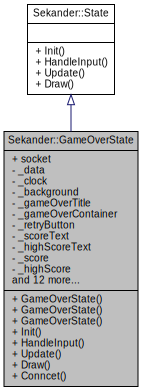
\includegraphics[width=214pt]{classSekander_1_1GameOverState__inherit__graph}
\end{center}
\end{figure}


Collaboration diagram for Sekander\+:\+:Game\+Over\+State\+:
\nopagebreak
\begin{figure}[H]
\begin{center}
\leavevmode
\includegraphics[height=550pt]{classSekander_1_1GameOverState__coll__graph}
\end{center}
\end{figure}
\subsection*{Public Member Functions}
\begin{DoxyCompactItemize}
\item 
\hyperlink{classSekander_1_1GameOverState_a8248a663f0624ca7f1c081cd0174b396}{Game\+Over\+State} (\hyperlink{namespaceSekander_a1d69b002ba2d23020901c28f0def5e16}{Game\+Data\+Ref} data, int score)
\item 
\hyperlink{classSekander_1_1GameOverState_a3e432a73ee48a8048c2d5a34226cae4b}{Game\+Over\+State} (\hyperlink{namespaceSekander_a1d69b002ba2d23020901c28f0def5e16}{Game\+Data\+Ref} data, int score, const char $\ast$xml\+\_\+\+D\+OC)
\item 
\hyperlink{classSekander_1_1GameOverState_aa856c012e9c97ac48360e089d39f0fb5}{Game\+Over\+State} (\hyperlink{namespaceSekander_a1d69b002ba2d23020901c28f0def5e16}{Game\+Data\+Ref} data, int score, const char $\ast$xml\+\_\+\+D\+OC, std\+::vector$<$ sf\+::\+Tcp\+Socket $\ast$$>$, bool, bool)
\item 
void \hyperlink{classSekander_1_1GameOverState_a1f0b4815da9cfb5221f2e3374b003de0}{Init} ()
\item 
void \hyperlink{classSekander_1_1GameOverState_ade27fc3af036b3c50df4ccf6cb795627}{Handle\+Input} ()
\item 
void \hyperlink{classSekander_1_1GameOverState_a00b3dcb61cb0342cf0fe4cc181e99b6b}{Update} (float dt)
\item 
void \hyperlink{classSekander_1_1GameOverState_af2407df4e95d8add41ed995157bc0905}{Draw} (float dt)
\item 
void \hyperlink{classSekander_1_1GameOverState_a577c6f01f9d687d772cefd17c2643e5f}{Conncet} ()
\end{DoxyCompactItemize}
\subsection*{Public Attributes}
\begin{DoxyCompactItemize}
\item 
sf\+::\+Tcp\+Socket \hyperlink{classSekander_1_1GameOverState_a664bfe46410e08bd6a9d399ac3e79dc3}{socket}
\end{DoxyCompactItemize}
\subsection*{Private Attributes}
\begin{DoxyCompactItemize}
\item 
\hyperlink{namespaceSekander_a1d69b002ba2d23020901c28f0def5e16}{Game\+Data\+Ref} \hyperlink{classSekander_1_1GameOverState_ac60174d0e0b62802ab2b0c05247d33b5}{\+\_\+data}
\item 
sf\+::\+Clock \hyperlink{classSekander_1_1GameOverState_a3b1c892e022575bd70cf97928d79b7da}{\+\_\+clock}
\item 
sf\+::\+Sprite \hyperlink{classSekander_1_1GameOverState_a250cf3a483960abc015415739067f6a5}{\+\_\+background}
\item 
sf\+::\+Sprite \hyperlink{classSekander_1_1GameOverState_a48e09487fe6fe308acbae0971d041710}{\+\_\+game\+Over\+Title}
\item 
sf\+::\+Sprite \hyperlink{classSekander_1_1GameOverState_ae699b96a7881e8852a2e64431ea5bda9}{\+\_\+game\+Over\+Container}
\item 
sf\+::\+Sprite \hyperlink{classSekander_1_1GameOverState_a1fc5e8938f774f4dc10d42b3876030ac}{\+\_\+retry\+Button}
\item 
sf\+::\+Text \hyperlink{classSekander_1_1GameOverState_adb60ef9a4d2fea746dfd3a9edf51d02b}{\+\_\+score\+Text}
\item 
sf\+::\+Text \hyperlink{classSekander_1_1GameOverState_afdd0049bf1354a13782e7ba21fb4befd}{\+\_\+high\+Score\+Text}
\item 
int \hyperlink{classSekander_1_1GameOverState_ad79b72fc4efc8b770422c2c16d07d6c3}{\+\_\+score}
\item 
int \hyperlink{classSekander_1_1GameOverState_ad7ba3fadc25c0470994d46ce91170108}{\+\_\+high\+Score}
\item 
int \hyperlink{classSekander_1_1GameOverState_ac04064783eaa87ca083beb919737635c}{\+\_\+temp\+\_\+score}
\item 
const char $\ast$ \hyperlink{classSekander_1_1GameOverState_a12cfdad7be4cb5ecc3d6678e1ed0b957}{\+\_\+xml\+\_\+\+D\+OC}
\item 
\hyperlink{classSekander_1_1LoadingGameObjects}{Loading\+Game\+Objects} $\ast$ \hyperlink{classSekander_1_1GameOverState_a5f0d39a093c067de484c17561f862de2}{ld}
\item 
sf\+::\+Rectangle\+Shape \hyperlink{classSekander_1_1GameOverState_aad418282474c59558d02e5b7f52a841c}{window\+\_\+rec}
\item 
sf\+::\+Rectangle\+Shape \hyperlink{classSekander_1_1GameOverState_afef7263e74fde41d6c779a473fd93105}{window\+\_\+rec2}
\item 
int \hyperlink{classSekander_1_1GameOverState_ac0f2e82316a36af6239ae24a03f2824f}{r} = 100
\item 
int \hyperlink{classSekander_1_1GameOverState_a48dbce2f5fb70dbaec0edf0d2de4aea6}{b} = 100
\item 
int \hyperlink{classSekander_1_1GameOverState_a7689bd10edad691528b434f0868c9e72}{g} = 0
\item 
int \hyperlink{classSekander_1_1GameOverState_a982c7e95494397743efa83e216ccd055}{a} = 255
\item 
int \hyperlink{classSekander_1_1GameOverState_aaf30770d2b2ab5f5be8a4d3443a2aa55}{a\+\_\+b} = 0
\item 
bool \hyperlink{classSekander_1_1GameOverState_a5656ae0aefaffa2409a51b1c3bd0f88c}{\+\_\+max}
\item 
bool \hyperlink{classSekander_1_1GameOverState_af8260bf3049c7b7cb7d2ea3781e3beae}{fade\+\_\+out}
\end{DoxyCompactItemize}


\subsection{Constructor \& Destructor Documentation}
\mbox{\Hypertarget{classSekander_1_1GameOverState_a8248a663f0624ca7f1c081cd0174b396}\label{classSekander_1_1GameOverState_a8248a663f0624ca7f1c081cd0174b396}} 
\index{Sekander\+::\+Game\+Over\+State@{Sekander\+::\+Game\+Over\+State}!Game\+Over\+State@{Game\+Over\+State}}
\index{Game\+Over\+State@{Game\+Over\+State}!Sekander\+::\+Game\+Over\+State@{Sekander\+::\+Game\+Over\+State}}
\subsubsection{\texorpdfstring{Game\+Over\+State()}{GameOverState()}\hspace{0.1cm}{\footnotesize\ttfamily [1/3]}}
{\footnotesize\ttfamily Sekander\+::\+Game\+Over\+State\+::\+Game\+Over\+State (\begin{DoxyParamCaption}\item[{\hyperlink{namespaceSekander_a1d69b002ba2d23020901c28f0def5e16}{Game\+Data\+Ref}}]{data,  }\item[{int}]{score }\end{DoxyParamCaption})}

\mbox{\Hypertarget{classSekander_1_1GameOverState_a3e432a73ee48a8048c2d5a34226cae4b}\label{classSekander_1_1GameOverState_a3e432a73ee48a8048c2d5a34226cae4b}} 
\index{Sekander\+::\+Game\+Over\+State@{Sekander\+::\+Game\+Over\+State}!Game\+Over\+State@{Game\+Over\+State}}
\index{Game\+Over\+State@{Game\+Over\+State}!Sekander\+::\+Game\+Over\+State@{Sekander\+::\+Game\+Over\+State}}
\subsubsection{\texorpdfstring{Game\+Over\+State()}{GameOverState()}\hspace{0.1cm}{\footnotesize\ttfamily [2/3]}}
{\footnotesize\ttfamily Sekander\+::\+Game\+Over\+State\+::\+Game\+Over\+State (\begin{DoxyParamCaption}\item[{\hyperlink{namespaceSekander_a1d69b002ba2d23020901c28f0def5e16}{Game\+Data\+Ref}}]{data,  }\item[{int}]{score,  }\item[{const char $\ast$}]{xml\+\_\+\+D\+OC }\end{DoxyParamCaption})}

\mbox{\Hypertarget{classSekander_1_1GameOverState_aa856c012e9c97ac48360e089d39f0fb5}\label{classSekander_1_1GameOverState_aa856c012e9c97ac48360e089d39f0fb5}} 
\index{Sekander\+::\+Game\+Over\+State@{Sekander\+::\+Game\+Over\+State}!Game\+Over\+State@{Game\+Over\+State}}
\index{Game\+Over\+State@{Game\+Over\+State}!Sekander\+::\+Game\+Over\+State@{Sekander\+::\+Game\+Over\+State}}
\subsubsection{\texorpdfstring{Game\+Over\+State()}{GameOverState()}\hspace{0.1cm}{\footnotesize\ttfamily [3/3]}}
{\footnotesize\ttfamily Sekander\+::\+Game\+Over\+State\+::\+Game\+Over\+State (\begin{DoxyParamCaption}\item[{\hyperlink{namespaceSekander_a1d69b002ba2d23020901c28f0def5e16}{Game\+Data\+Ref}}]{data,  }\item[{int}]{score,  }\item[{const char $\ast$}]{xml\+\_\+\+D\+OC,  }\item[{std\+::vector$<$ sf\+::\+Tcp\+Socket $\ast$$>$}]{socket\+\_\+list,  }\item[{bool}]{i\+\_\+am\+\_\+the\+\_\+\+H\+O\+ST,  }\item[{bool}]{i\+\_\+am\+\_\+the\+\_\+\+C\+L\+I\+E\+NT }\end{DoxyParamCaption})}



\subsection{Member Function Documentation}
\mbox{\Hypertarget{classSekander_1_1GameOverState_a577c6f01f9d687d772cefd17c2643e5f}\label{classSekander_1_1GameOverState_a577c6f01f9d687d772cefd17c2643e5f}} 
\index{Sekander\+::\+Game\+Over\+State@{Sekander\+::\+Game\+Over\+State}!Conncet@{Conncet}}
\index{Conncet@{Conncet}!Sekander\+::\+Game\+Over\+State@{Sekander\+::\+Game\+Over\+State}}
\subsubsection{\texorpdfstring{Conncet()}{Conncet()}}
{\footnotesize\ttfamily void Sekander\+::\+Game\+Over\+State\+::\+Conncet (\begin{DoxyParamCaption}{ }\end{DoxyParamCaption})\hspace{0.3cm}{\ttfamily [inline]}}

\mbox{\Hypertarget{classSekander_1_1GameOverState_af2407df4e95d8add41ed995157bc0905}\label{classSekander_1_1GameOverState_af2407df4e95d8add41ed995157bc0905}} 
\index{Sekander\+::\+Game\+Over\+State@{Sekander\+::\+Game\+Over\+State}!Draw@{Draw}}
\index{Draw@{Draw}!Sekander\+::\+Game\+Over\+State@{Sekander\+::\+Game\+Over\+State}}
\subsubsection{\texorpdfstring{Draw()}{Draw()}}
{\footnotesize\ttfamily void Sekander\+::\+Game\+Over\+State\+::\+Draw (\begin{DoxyParamCaption}\item[{float}]{dt }\end{DoxyParamCaption})\hspace{0.3cm}{\ttfamily [virtual]}}



Implements \hyperlink{classSekander_1_1State_a6ae7c2de1985461232a3ad694ca736b5}{Sekander\+::\+State}.

\mbox{\Hypertarget{classSekander_1_1GameOverState_ade27fc3af036b3c50df4ccf6cb795627}\label{classSekander_1_1GameOverState_ade27fc3af036b3c50df4ccf6cb795627}} 
\index{Sekander\+::\+Game\+Over\+State@{Sekander\+::\+Game\+Over\+State}!Handle\+Input@{Handle\+Input}}
\index{Handle\+Input@{Handle\+Input}!Sekander\+::\+Game\+Over\+State@{Sekander\+::\+Game\+Over\+State}}
\subsubsection{\texorpdfstring{Handle\+Input()}{HandleInput()}}
{\footnotesize\ttfamily void Sekander\+::\+Game\+Over\+State\+::\+Handle\+Input (\begin{DoxyParamCaption}{ }\end{DoxyParamCaption})\hspace{0.3cm}{\ttfamily [virtual]}}



Implements \hyperlink{classSekander_1_1State_ad55ae42f5887db5745fda9f2bd30aaa3}{Sekander\+::\+State}.

\mbox{\Hypertarget{classSekander_1_1GameOverState_a1f0b4815da9cfb5221f2e3374b003de0}\label{classSekander_1_1GameOverState_a1f0b4815da9cfb5221f2e3374b003de0}} 
\index{Sekander\+::\+Game\+Over\+State@{Sekander\+::\+Game\+Over\+State}!Init@{Init}}
\index{Init@{Init}!Sekander\+::\+Game\+Over\+State@{Sekander\+::\+Game\+Over\+State}}
\subsubsection{\texorpdfstring{Init()}{Init()}}
{\footnotesize\ttfamily void Sekander\+::\+Game\+Over\+State\+::\+Init (\begin{DoxyParamCaption}{ }\end{DoxyParamCaption})\hspace{0.3cm}{\ttfamily [virtual]}}



Implements \hyperlink{classSekander_1_1State_a171be4b77d4c13e01849b867bd3fa8f5}{Sekander\+::\+State}.

\mbox{\Hypertarget{classSekander_1_1GameOverState_a00b3dcb61cb0342cf0fe4cc181e99b6b}\label{classSekander_1_1GameOverState_a00b3dcb61cb0342cf0fe4cc181e99b6b}} 
\index{Sekander\+::\+Game\+Over\+State@{Sekander\+::\+Game\+Over\+State}!Update@{Update}}
\index{Update@{Update}!Sekander\+::\+Game\+Over\+State@{Sekander\+::\+Game\+Over\+State}}
\subsubsection{\texorpdfstring{Update()}{Update()}}
{\footnotesize\ttfamily void Sekander\+::\+Game\+Over\+State\+::\+Update (\begin{DoxyParamCaption}\item[{float}]{dt }\end{DoxyParamCaption})\hspace{0.3cm}{\ttfamily [virtual]}}



Implements \hyperlink{classSekander_1_1State_a08d49e399db6f68247f410f7fddc7963}{Sekander\+::\+State}.



\subsection{Member Data Documentation}
\mbox{\Hypertarget{classSekander_1_1GameOverState_a250cf3a483960abc015415739067f6a5}\label{classSekander_1_1GameOverState_a250cf3a483960abc015415739067f6a5}} 
\index{Sekander\+::\+Game\+Over\+State@{Sekander\+::\+Game\+Over\+State}!\+\_\+background@{\+\_\+background}}
\index{\+\_\+background@{\+\_\+background}!Sekander\+::\+Game\+Over\+State@{Sekander\+::\+Game\+Over\+State}}
\subsubsection{\texorpdfstring{\+\_\+background}{\_background}}
{\footnotesize\ttfamily sf\+::\+Sprite Sekander\+::\+Game\+Over\+State\+::\+\_\+background\hspace{0.3cm}{\ttfamily [private]}}

\mbox{\Hypertarget{classSekander_1_1GameOverState_a3b1c892e022575bd70cf97928d79b7da}\label{classSekander_1_1GameOverState_a3b1c892e022575bd70cf97928d79b7da}} 
\index{Sekander\+::\+Game\+Over\+State@{Sekander\+::\+Game\+Over\+State}!\+\_\+clock@{\+\_\+clock}}
\index{\+\_\+clock@{\+\_\+clock}!Sekander\+::\+Game\+Over\+State@{Sekander\+::\+Game\+Over\+State}}
\subsubsection{\texorpdfstring{\+\_\+clock}{\_clock}}
{\footnotesize\ttfamily sf\+::\+Clock Sekander\+::\+Game\+Over\+State\+::\+\_\+clock\hspace{0.3cm}{\ttfamily [private]}}

\mbox{\Hypertarget{classSekander_1_1GameOverState_ac60174d0e0b62802ab2b0c05247d33b5}\label{classSekander_1_1GameOverState_ac60174d0e0b62802ab2b0c05247d33b5}} 
\index{Sekander\+::\+Game\+Over\+State@{Sekander\+::\+Game\+Over\+State}!\+\_\+data@{\+\_\+data}}
\index{\+\_\+data@{\+\_\+data}!Sekander\+::\+Game\+Over\+State@{Sekander\+::\+Game\+Over\+State}}
\subsubsection{\texorpdfstring{\+\_\+data}{\_data}}
{\footnotesize\ttfamily \hyperlink{namespaceSekander_a1d69b002ba2d23020901c28f0def5e16}{Game\+Data\+Ref} Sekander\+::\+Game\+Over\+State\+::\+\_\+data\hspace{0.3cm}{\ttfamily [private]}}

\mbox{\Hypertarget{classSekander_1_1GameOverState_ae699b96a7881e8852a2e64431ea5bda9}\label{classSekander_1_1GameOverState_ae699b96a7881e8852a2e64431ea5bda9}} 
\index{Sekander\+::\+Game\+Over\+State@{Sekander\+::\+Game\+Over\+State}!\+\_\+game\+Over\+Container@{\+\_\+game\+Over\+Container}}
\index{\+\_\+game\+Over\+Container@{\+\_\+game\+Over\+Container}!Sekander\+::\+Game\+Over\+State@{Sekander\+::\+Game\+Over\+State}}
\subsubsection{\texorpdfstring{\+\_\+game\+Over\+Container}{\_gameOverContainer}}
{\footnotesize\ttfamily sf\+::\+Sprite Sekander\+::\+Game\+Over\+State\+::\+\_\+game\+Over\+Container\hspace{0.3cm}{\ttfamily [private]}}

\mbox{\Hypertarget{classSekander_1_1GameOverState_a48e09487fe6fe308acbae0971d041710}\label{classSekander_1_1GameOverState_a48e09487fe6fe308acbae0971d041710}} 
\index{Sekander\+::\+Game\+Over\+State@{Sekander\+::\+Game\+Over\+State}!\+\_\+game\+Over\+Title@{\+\_\+game\+Over\+Title}}
\index{\+\_\+game\+Over\+Title@{\+\_\+game\+Over\+Title}!Sekander\+::\+Game\+Over\+State@{Sekander\+::\+Game\+Over\+State}}
\subsubsection{\texorpdfstring{\+\_\+game\+Over\+Title}{\_gameOverTitle}}
{\footnotesize\ttfamily sf\+::\+Sprite Sekander\+::\+Game\+Over\+State\+::\+\_\+game\+Over\+Title\hspace{0.3cm}{\ttfamily [private]}}

\mbox{\Hypertarget{classSekander_1_1GameOverState_ad7ba3fadc25c0470994d46ce91170108}\label{classSekander_1_1GameOverState_ad7ba3fadc25c0470994d46ce91170108}} 
\index{Sekander\+::\+Game\+Over\+State@{Sekander\+::\+Game\+Over\+State}!\+\_\+high\+Score@{\+\_\+high\+Score}}
\index{\+\_\+high\+Score@{\+\_\+high\+Score}!Sekander\+::\+Game\+Over\+State@{Sekander\+::\+Game\+Over\+State}}
\subsubsection{\texorpdfstring{\+\_\+high\+Score}{\_highScore}}
{\footnotesize\ttfamily int Sekander\+::\+Game\+Over\+State\+::\+\_\+high\+Score\hspace{0.3cm}{\ttfamily [private]}}

\mbox{\Hypertarget{classSekander_1_1GameOverState_afdd0049bf1354a13782e7ba21fb4befd}\label{classSekander_1_1GameOverState_afdd0049bf1354a13782e7ba21fb4befd}} 
\index{Sekander\+::\+Game\+Over\+State@{Sekander\+::\+Game\+Over\+State}!\+\_\+high\+Score\+Text@{\+\_\+high\+Score\+Text}}
\index{\+\_\+high\+Score\+Text@{\+\_\+high\+Score\+Text}!Sekander\+::\+Game\+Over\+State@{Sekander\+::\+Game\+Over\+State}}
\subsubsection{\texorpdfstring{\+\_\+high\+Score\+Text}{\_highScoreText}}
{\footnotesize\ttfamily sf\+::\+Text Sekander\+::\+Game\+Over\+State\+::\+\_\+high\+Score\+Text\hspace{0.3cm}{\ttfamily [private]}}

\mbox{\Hypertarget{classSekander_1_1GameOverState_a5656ae0aefaffa2409a51b1c3bd0f88c}\label{classSekander_1_1GameOverState_a5656ae0aefaffa2409a51b1c3bd0f88c}} 
\index{Sekander\+::\+Game\+Over\+State@{Sekander\+::\+Game\+Over\+State}!\+\_\+max@{\+\_\+max}}
\index{\+\_\+max@{\+\_\+max}!Sekander\+::\+Game\+Over\+State@{Sekander\+::\+Game\+Over\+State}}
\subsubsection{\texorpdfstring{\+\_\+max}{\_max}}
{\footnotesize\ttfamily bool Sekander\+::\+Game\+Over\+State\+::\+\_\+max\hspace{0.3cm}{\ttfamily [private]}}

\mbox{\Hypertarget{classSekander_1_1GameOverState_a1fc5e8938f774f4dc10d42b3876030ac}\label{classSekander_1_1GameOverState_a1fc5e8938f774f4dc10d42b3876030ac}} 
\index{Sekander\+::\+Game\+Over\+State@{Sekander\+::\+Game\+Over\+State}!\+\_\+retry\+Button@{\+\_\+retry\+Button}}
\index{\+\_\+retry\+Button@{\+\_\+retry\+Button}!Sekander\+::\+Game\+Over\+State@{Sekander\+::\+Game\+Over\+State}}
\subsubsection{\texorpdfstring{\+\_\+retry\+Button}{\_retryButton}}
{\footnotesize\ttfamily sf\+::\+Sprite Sekander\+::\+Game\+Over\+State\+::\+\_\+retry\+Button\hspace{0.3cm}{\ttfamily [private]}}

\mbox{\Hypertarget{classSekander_1_1GameOverState_ad79b72fc4efc8b770422c2c16d07d6c3}\label{classSekander_1_1GameOverState_ad79b72fc4efc8b770422c2c16d07d6c3}} 
\index{Sekander\+::\+Game\+Over\+State@{Sekander\+::\+Game\+Over\+State}!\+\_\+score@{\+\_\+score}}
\index{\+\_\+score@{\+\_\+score}!Sekander\+::\+Game\+Over\+State@{Sekander\+::\+Game\+Over\+State}}
\subsubsection{\texorpdfstring{\+\_\+score}{\_score}}
{\footnotesize\ttfamily int Sekander\+::\+Game\+Over\+State\+::\+\_\+score\hspace{0.3cm}{\ttfamily [private]}}

\mbox{\Hypertarget{classSekander_1_1GameOverState_adb60ef9a4d2fea746dfd3a9edf51d02b}\label{classSekander_1_1GameOverState_adb60ef9a4d2fea746dfd3a9edf51d02b}} 
\index{Sekander\+::\+Game\+Over\+State@{Sekander\+::\+Game\+Over\+State}!\+\_\+score\+Text@{\+\_\+score\+Text}}
\index{\+\_\+score\+Text@{\+\_\+score\+Text}!Sekander\+::\+Game\+Over\+State@{Sekander\+::\+Game\+Over\+State}}
\subsubsection{\texorpdfstring{\+\_\+score\+Text}{\_scoreText}}
{\footnotesize\ttfamily sf\+::\+Text Sekander\+::\+Game\+Over\+State\+::\+\_\+score\+Text\hspace{0.3cm}{\ttfamily [private]}}

\mbox{\Hypertarget{classSekander_1_1GameOverState_ac04064783eaa87ca083beb919737635c}\label{classSekander_1_1GameOverState_ac04064783eaa87ca083beb919737635c}} 
\index{Sekander\+::\+Game\+Over\+State@{Sekander\+::\+Game\+Over\+State}!\+\_\+temp\+\_\+score@{\+\_\+temp\+\_\+score}}
\index{\+\_\+temp\+\_\+score@{\+\_\+temp\+\_\+score}!Sekander\+::\+Game\+Over\+State@{Sekander\+::\+Game\+Over\+State}}
\subsubsection{\texorpdfstring{\+\_\+temp\+\_\+score}{\_temp\_score}}
{\footnotesize\ttfamily int Sekander\+::\+Game\+Over\+State\+::\+\_\+temp\+\_\+score\hspace{0.3cm}{\ttfamily [private]}}

\mbox{\Hypertarget{classSekander_1_1GameOverState_a12cfdad7be4cb5ecc3d6678e1ed0b957}\label{classSekander_1_1GameOverState_a12cfdad7be4cb5ecc3d6678e1ed0b957}} 
\index{Sekander\+::\+Game\+Over\+State@{Sekander\+::\+Game\+Over\+State}!\+\_\+xml\+\_\+\+D\+OC@{\+\_\+xml\+\_\+\+D\+OC}}
\index{\+\_\+xml\+\_\+\+D\+OC@{\+\_\+xml\+\_\+\+D\+OC}!Sekander\+::\+Game\+Over\+State@{Sekander\+::\+Game\+Over\+State}}
\subsubsection{\texorpdfstring{\+\_\+xml\+\_\+\+D\+OC}{\_xml\_DOC}}
{\footnotesize\ttfamily const char$\ast$ Sekander\+::\+Game\+Over\+State\+::\+\_\+xml\+\_\+\+D\+OC\hspace{0.3cm}{\ttfamily [private]}}

\mbox{\Hypertarget{classSekander_1_1GameOverState_a982c7e95494397743efa83e216ccd055}\label{classSekander_1_1GameOverState_a982c7e95494397743efa83e216ccd055}} 
\index{Sekander\+::\+Game\+Over\+State@{Sekander\+::\+Game\+Over\+State}!a@{a}}
\index{a@{a}!Sekander\+::\+Game\+Over\+State@{Sekander\+::\+Game\+Over\+State}}
\subsubsection{\texorpdfstring{a}{a}}
{\footnotesize\ttfamily int Sekander\+::\+Game\+Over\+State\+::a = 255\hspace{0.3cm}{\ttfamily [private]}}

\mbox{\Hypertarget{classSekander_1_1GameOverState_aaf30770d2b2ab5f5be8a4d3443a2aa55}\label{classSekander_1_1GameOverState_aaf30770d2b2ab5f5be8a4d3443a2aa55}} 
\index{Sekander\+::\+Game\+Over\+State@{Sekander\+::\+Game\+Over\+State}!a\+\_\+b@{a\+\_\+b}}
\index{a\+\_\+b@{a\+\_\+b}!Sekander\+::\+Game\+Over\+State@{Sekander\+::\+Game\+Over\+State}}
\subsubsection{\texorpdfstring{a\+\_\+b}{a\_b}}
{\footnotesize\ttfamily int Sekander\+::\+Game\+Over\+State\+::a\+\_\+b = 0\hspace{0.3cm}{\ttfamily [private]}}

\mbox{\Hypertarget{classSekander_1_1GameOverState_a48dbce2f5fb70dbaec0edf0d2de4aea6}\label{classSekander_1_1GameOverState_a48dbce2f5fb70dbaec0edf0d2de4aea6}} 
\index{Sekander\+::\+Game\+Over\+State@{Sekander\+::\+Game\+Over\+State}!b@{b}}
\index{b@{b}!Sekander\+::\+Game\+Over\+State@{Sekander\+::\+Game\+Over\+State}}
\subsubsection{\texorpdfstring{b}{b}}
{\footnotesize\ttfamily int Sekander\+::\+Game\+Over\+State\+::b = 100\hspace{0.3cm}{\ttfamily [private]}}

\mbox{\Hypertarget{classSekander_1_1GameOverState_af8260bf3049c7b7cb7d2ea3781e3beae}\label{classSekander_1_1GameOverState_af8260bf3049c7b7cb7d2ea3781e3beae}} 
\index{Sekander\+::\+Game\+Over\+State@{Sekander\+::\+Game\+Over\+State}!fade\+\_\+out@{fade\+\_\+out}}
\index{fade\+\_\+out@{fade\+\_\+out}!Sekander\+::\+Game\+Over\+State@{Sekander\+::\+Game\+Over\+State}}
\subsubsection{\texorpdfstring{fade\+\_\+out}{fade\_out}}
{\footnotesize\ttfamily bool Sekander\+::\+Game\+Over\+State\+::fade\+\_\+out\hspace{0.3cm}{\ttfamily [private]}}

\mbox{\Hypertarget{classSekander_1_1GameOverState_a7689bd10edad691528b434f0868c9e72}\label{classSekander_1_1GameOverState_a7689bd10edad691528b434f0868c9e72}} 
\index{Sekander\+::\+Game\+Over\+State@{Sekander\+::\+Game\+Over\+State}!g@{g}}
\index{g@{g}!Sekander\+::\+Game\+Over\+State@{Sekander\+::\+Game\+Over\+State}}
\subsubsection{\texorpdfstring{g}{g}}
{\footnotesize\ttfamily int Sekander\+::\+Game\+Over\+State\+::g = 0\hspace{0.3cm}{\ttfamily [private]}}

\mbox{\Hypertarget{classSekander_1_1GameOverState_a5f0d39a093c067de484c17561f862de2}\label{classSekander_1_1GameOverState_a5f0d39a093c067de484c17561f862de2}} 
\index{Sekander\+::\+Game\+Over\+State@{Sekander\+::\+Game\+Over\+State}!ld@{ld}}
\index{ld@{ld}!Sekander\+::\+Game\+Over\+State@{Sekander\+::\+Game\+Over\+State}}
\subsubsection{\texorpdfstring{ld}{ld}}
{\footnotesize\ttfamily \hyperlink{classSekander_1_1LoadingGameObjects}{Loading\+Game\+Objects}$\ast$ Sekander\+::\+Game\+Over\+State\+::ld\hspace{0.3cm}{\ttfamily [private]}}

\mbox{\Hypertarget{classSekander_1_1GameOverState_ac0f2e82316a36af6239ae24a03f2824f}\label{classSekander_1_1GameOverState_ac0f2e82316a36af6239ae24a03f2824f}} 
\index{Sekander\+::\+Game\+Over\+State@{Sekander\+::\+Game\+Over\+State}!r@{r}}
\index{r@{r}!Sekander\+::\+Game\+Over\+State@{Sekander\+::\+Game\+Over\+State}}
\subsubsection{\texorpdfstring{r}{r}}
{\footnotesize\ttfamily int Sekander\+::\+Game\+Over\+State\+::r = 100\hspace{0.3cm}{\ttfamily [private]}}

\mbox{\Hypertarget{classSekander_1_1GameOverState_a664bfe46410e08bd6a9d399ac3e79dc3}\label{classSekander_1_1GameOverState_a664bfe46410e08bd6a9d399ac3e79dc3}} 
\index{Sekander\+::\+Game\+Over\+State@{Sekander\+::\+Game\+Over\+State}!socket@{socket}}
\index{socket@{socket}!Sekander\+::\+Game\+Over\+State@{Sekander\+::\+Game\+Over\+State}}
\subsubsection{\texorpdfstring{socket}{socket}}
{\footnotesize\ttfamily sf\+::\+Tcp\+Socket Sekander\+::\+Game\+Over\+State\+::socket}

\mbox{\Hypertarget{classSekander_1_1GameOverState_aad418282474c59558d02e5b7f52a841c}\label{classSekander_1_1GameOverState_aad418282474c59558d02e5b7f52a841c}} 
\index{Sekander\+::\+Game\+Over\+State@{Sekander\+::\+Game\+Over\+State}!window\+\_\+rec@{window\+\_\+rec}}
\index{window\+\_\+rec@{window\+\_\+rec}!Sekander\+::\+Game\+Over\+State@{Sekander\+::\+Game\+Over\+State}}
\subsubsection{\texorpdfstring{window\+\_\+rec}{window\_rec}}
{\footnotesize\ttfamily sf\+::\+Rectangle\+Shape Sekander\+::\+Game\+Over\+State\+::window\+\_\+rec\hspace{0.3cm}{\ttfamily [private]}}

\mbox{\Hypertarget{classSekander_1_1GameOverState_afef7263e74fde41d6c779a473fd93105}\label{classSekander_1_1GameOverState_afef7263e74fde41d6c779a473fd93105}} 
\index{Sekander\+::\+Game\+Over\+State@{Sekander\+::\+Game\+Over\+State}!window\+\_\+rec2@{window\+\_\+rec2}}
\index{window\+\_\+rec2@{window\+\_\+rec2}!Sekander\+::\+Game\+Over\+State@{Sekander\+::\+Game\+Over\+State}}
\subsubsection{\texorpdfstring{window\+\_\+rec2}{window\_rec2}}
{\footnotesize\ttfamily sf\+::\+Rectangle\+Shape Sekander\+::\+Game\+Over\+State\+::window\+\_\+rec2\hspace{0.3cm}{\ttfamily [private]}}



The documentation for this class was generated from the following files\+:\begin{DoxyCompactItemize}
\item 
/mnt/hdd/\+C0de/\+Engines/\+S\+F\+M\+L/\+S\+F\+M\+L\+\_\+\+Engine/include/\hyperlink{GameOverState_8hpp}{Game\+Over\+State.\+hpp}\item 
/mnt/hdd/\+C0de/\+Engines/\+S\+F\+M\+L/\+S\+F\+M\+L\+\_\+\+Engine/src/\hyperlink{GameOverState_8cpp}{Game\+Over\+State.\+cpp}\end{DoxyCompactItemize}

\hypertarget{classSekander_1_1GameState}{}\section{Sekander\+:\+:Game\+State Class Reference}
\label{classSekander_1_1GameState}\index{Sekander\+::\+Game\+State@{Sekander\+::\+Game\+State}}


{\ttfamily \#include $<$Game\+State.\+hpp$>$}



Inheritance diagram for Sekander\+:\+:Game\+State\+:
\nopagebreak
\begin{figure}[H]
\begin{center}
\leavevmode
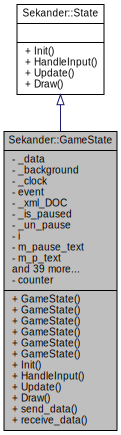
\includegraphics[width=193pt]{classSekander_1_1GameState__inherit__graph}
\end{center}
\end{figure}


Collaboration diagram for Sekander\+:\+:Game\+State\+:
\nopagebreak
\begin{figure}[H]
\begin{center}
\leavevmode
\includegraphics[width=350pt]{classSekander_1_1GameState__coll__graph}
\end{center}
\end{figure}
\subsection*{Public Member Functions}
\begin{DoxyCompactItemize}
\item 
\hyperlink{classSekander_1_1GameState_af47a4f5c384bf320048bea9b95b854ea}{Game\+State} (\hyperlink{namespaceSekander_a1d69b002ba2d23020901c28f0def5e16}{Game\+Data\+Ref} \hyperlink{classSekander_1_1GameState_ab267d83dd406910063033004946c83e3}{data})
\item 
\hyperlink{classSekander_1_1GameState_a6003e8f7b7ed16e9cd005972c1738714}{Game\+State} (\hyperlink{namespaceSekander_a1d69b002ba2d23020901c28f0def5e16}{Game\+Data\+Ref} \hyperlink{classSekander_1_1GameState_ab267d83dd406910063033004946c83e3}{data}, const char $\ast$xml\+\_\+\+D\+OC)
\item 
\hyperlink{classSekander_1_1GameState_ada3b0410f31b43c596dfbaf729e82546}{Game\+State} (\hyperlink{namespaceSekander_a1d69b002ba2d23020901c28f0def5e16}{Game\+Data\+Ref} \hyperlink{classSekander_1_1GameState_ab267d83dd406910063033004946c83e3}{data}, const char $\ast$xml\+\_\+\+D\+OC, sf\+::\+Tcp\+Socket $\ast$socket)
\item 
\hyperlink{classSekander_1_1GameState_a00cf0995110149d2e86240bd7514b141}{Game\+State} (\hyperlink{namespaceSekander_a1d69b002ba2d23020901c28f0def5e16}{Game\+Data\+Ref} \hyperlink{classSekander_1_1GameState_ab267d83dd406910063033004946c83e3}{data}, const char $\ast$xml\+\_\+\+D\+OC, sf\+::\+Tcp\+Socket $\ast$socket, sf\+::\+Tcp\+Socket $\ast$\hyperlink{classSekander_1_1GameState_a4096b6555a755229b11091167b02c1f9}{client})
\item 
\hyperlink{classSekander_1_1GameState_acbb55fb2bbaee0294648eb7ea6ab6193}{Game\+State} (\hyperlink{namespaceSekander_a1d69b002ba2d23020901c28f0def5e16}{Game\+Data\+Ref} \hyperlink{classSekander_1_1GameState_ab267d83dd406910063033004946c83e3}{data}, const char $\ast$xml\+\_\+\+D\+OC, sf\+::\+Tcp\+Socket $\ast$socket, sf\+::\+Tcp\+Socket $\ast$\hyperlink{classSekander_1_1GameState_a4096b6555a755229b11091167b02c1f9}{client}, bool, bool)
\item 
\hyperlink{classSekander_1_1GameState_a80541160bcb4bc8edbc1a54bff777817}{Game\+State} (\hyperlink{namespaceSekander_a1d69b002ba2d23020901c28f0def5e16}{Game\+Data\+Ref} \hyperlink{classSekander_1_1GameState_ab267d83dd406910063033004946c83e3}{data}, const char $\ast$xml\+\_\+\+D\+OC, std\+::vector$<$ sf\+::\+Tcp\+Socket $\ast$$>$, bool, bool)
\item 
void \hyperlink{classSekander_1_1GameState_af27f06a5535b1fbc2f52299a1eb3bee2}{Init} ()
\item 
void \hyperlink{classSekander_1_1GameState_ab3e0961a77a513cdc49fe8e6b3962280}{Handle\+Input} ()
\item 
void \hyperlink{classSekander_1_1GameState_ac04d512257bd38244f2d6d1484aa9040}{Update} (float dt)
\item 
void \hyperlink{classSekander_1_1GameState_ae940d623e220e069c6574810c5d083be}{Draw} (float dt)
\item 
void \hyperlink{classSekander_1_1GameState_a56d41e63267e7c6b2489c6940de0a402}{send\+\_\+data} ()
\item 
void \hyperlink{classSekander_1_1GameState_ae10726ccc07765dd37eae75c55ef9a39}{receive\+\_\+data} ()
\end{DoxyCompactItemize}
\subsection*{Private Attributes}
\begin{DoxyCompactItemize}
\item 
\hyperlink{namespaceSekander_a1d69b002ba2d23020901c28f0def5e16}{Game\+Data\+Ref} \hyperlink{classSekander_1_1GameState_a8d4871b8f695026f712a631f4d15a7bc}{\+\_\+data}
\item 
sf\+::\+Sprite \hyperlink{classSekander_1_1GameState_ac757f96251226e5d5cd07b8c75671299}{\+\_\+background}
\item 
sf\+::\+Clock \hyperlink{classSekander_1_1GameState_a3ed5ec609d3994afe8b25a6b3359abb7}{\+\_\+clock}
\item 
sf\+::\+Event \hyperlink{classSekander_1_1GameState_a51627fd89906e418c311a4853e7509ed}{event}
\item 
const char $\ast$ \hyperlink{classSekander_1_1GameState_a664c380e695b82fb68aead1cd9828282}{\+\_\+xml\+\_\+\+D\+OC}
\item 
bool \hyperlink{classSekander_1_1GameState_a64afed7f84d58d0b0d52752b33969ba2}{\+\_\+is\+\_\+paused}
\item 
bool \hyperlink{classSekander_1_1GameState_ace01a1a5682f32d83ddc4308c2dd5a0a}{\+\_\+un\+\_\+pause}
\item 
int \hyperlink{classSekander_1_1GameState_a9017176374407458e6fe4b0369ae63ba}{i} = 0
\item 
sf\+::\+Text \hyperlink{classSekander_1_1GameState_a9e4007a56ece8fb04e344198f3f00681}{m\+\_\+pause\+\_\+text}
\item 
sf\+::\+Text \hyperlink{classSekander_1_1GameState_ab8a913dd7ad77c86fd2588ab3cea7a3d}{m\+\_\+p\+\_\+text}
\item 
sf\+::\+Text \hyperlink{classSekander_1_1GameState_a6eae10c82abd67f0c5f277d476040fa7}{m\+\_\+a\+\_\+text}
\item 
sf\+::\+Text \hyperlink{classSekander_1_1GameState_a4d4f6d805ef4f5964cfa985c9eb49863}{m\+\_\+u\+\_\+text}
\item 
sf\+::\+Text \hyperlink{classSekander_1_1GameState_a003a29119d0c6036f48f6629c310e982}{m\+\_\+s\+\_\+text}
\item 
sf\+::\+Text \hyperlink{classSekander_1_1GameState_a5e1efc74f4b4c89981980762f7746188}{m\+\_\+e\+\_\+text}
\item 
char \hyperlink{classSekander_1_1GameState_ab267d83dd406910063033004946c83e3}{data} \mbox{[}100\mbox{]}
\item 
std\+::size\+\_\+t \hyperlink{classSekander_1_1GameState_a274e8d0ee8913f96c2973b34425c6d7f}{received}
\item 
sf\+::\+Tcp\+Socket $\ast$ \hyperlink{classSekander_1_1GameState_a2e6284526beda16cd853f964709a1dde}{game\+\_\+socket}
\item 
sf\+::\+Tcp\+Socket $\ast$ \hyperlink{classSekander_1_1GameState_ae85e17486292dcebc783c4cff136aea6}{game\+\_\+client}
\item 
std\+::vector$<$ sf\+::\+Tcp\+Socket $\ast$ $>$ \hyperlink{classSekander_1_1GameState_a930e32721a40b8e9f8eeaef3d1da9852}{\+\_\+socket\+\_\+list}
\item 
bool \hyperlink{classSekander_1_1GameState_aa0e1e7537cad0505a0ff751a5bca1cf3}{host}
\item 
bool \hyperlink{classSekander_1_1GameState_a4096b6555a755229b11091167b02c1f9}{client}
\item 
bool \hyperlink{classSekander_1_1GameState_a3f0cf150c794b1371bf2a20bf29d8463}{network\+\_\+game}
\item 
\hyperlink{classSekander_1_1LoadingGameObjects}{Loading\+Game\+Objects} $\ast$ \hyperlink{classSekander_1_1GameState_ad0cf3bf4943c3f025a9d46d1afc8f4ab}{ld}
\item 
\hyperlink{classSekander_1_1HUD}{H\+UD} $\ast$ \hyperlink{classSekander_1_1GameState_ab15428b5c508516dfb67eb4b5cdc313d}{hud}
\item 
int \hyperlink{classSekander_1_1GameState_a628790c63ef07329a39c322f370e52db}{\+\_\+game\+State}
\item 
int \hyperlink{classSekander_1_1GameState_a1722679ccb49b683a33dafbcc9cca6d7}{\+\_\+current\+\_\+state}
\item 
int \hyperlink{classSekander_1_1GameState_ac8ac6b28d48f95b723ec17ae37f7509e}{\+\_\+score}
\item 
tmx\+::\+Map \hyperlink{classSekander_1_1GameState_aa259af22c10b0f71cedc50c90a13b6ce}{map}
\item 
\hyperlink{classMapLayer}{Map\+Layer} $\ast$ \hyperlink{classSekander_1_1GameState_ae5ef3760e93eaa779734d0287dcca4fb}{layer1}
\item 
\hyperlink{classMapLayer}{Map\+Layer} $\ast$ \hyperlink{classSekander_1_1GameState_a4a24b0070e7d22098f6b057964cb0a91}{layer2}
\item 
\hyperlink{classMapLayer}{Map\+Layer} $\ast$ \hyperlink{classSekander_1_1GameState_aa6f018f199cabb2f40721403c62b308a}{layer3}
\item 
\hyperlink{classMapLayer}{Map\+Layer} $\ast$ \hyperlink{classSekander_1_1GameState_a69bd6996c7e1a849f95679bf93472407}{layer4}
\item 
b2\+Vec2 \hyperlink{classSekander_1_1GameState_a3967f08ea45421b5c4ec1a4e6fd1116b}{\+\_\+game\+Screen} = b2\+Vec2(\hyperlink{DEFINITIONS_8hpp_a6974d08a74da681b3957b2fead2608b8}{S\+C\+R\+E\+E\+N\+\_\+\+H\+E\+I\+G\+HT}, \hyperlink{DEFINITIONS_8hpp_a2cd109632a6dcccaa80b43561b1ab700}{S\+C\+R\+E\+E\+N\+\_\+\+W\+I\+D\+TH})
\item 
bool \hyperlink{classSekander_1_1GameState_ad03cd6358b24a3559c71eb904df73d5f}{is\+Key\+Released}
\item 
sf\+::\+View \hyperlink{classSekander_1_1GameState_ae5db885953e773fdbce4faf6ad03d480}{main\+\_\+view} = \hyperlink{classSekander_1_1GameState_a8d4871b8f695026f712a631f4d15a7bc}{\+\_\+data}-\/$>$window.\+get\+Default\+View()
\item 
sf\+::\+View \hyperlink{classSekander_1_1GameState_a4eacd2ce75969c80fc68be5fecd97c70}{minimap\+View}
\item 
sf\+::\+Rectangle\+Shape \hyperlink{classSekander_1_1GameState_add4fe356184898f68a463d3d7b06303f}{back}
\item 
sf\+::\+Rectangle\+Shape \hyperlink{classSekander_1_1GameState_a3b73733184431654c40332cf76735265}{rect}
\item 
sf\+::\+Rectangle\+Shape \hyperlink{classSekander_1_1GameState_a2ee11887ef73fd6176d8d2ce8ef3c110}{pause\+\_\+window\+\_\+rec}
\item 
sf\+::\+Rectangle\+Shape \hyperlink{classSekander_1_1GameState_a5286183d60d019bb4a2883e46a183b86}{debug\+\_\+rec}
\item 
int \hyperlink{classSekander_1_1GameState_a0d3ea2a26abb6cd10c3e493381400ada}{r} = 100
\item 
int \hyperlink{classSekander_1_1GameState_a6985b7cdb15e9be323ccc856379c15bb}{b} = 255
\item 
int \hyperlink{classSekander_1_1GameState_a31e0ac873c64d342e1d010e12edc0e22}{g} = 0
\item 
sf\+::\+Rectangle\+Shape \hyperlink{classSekander_1_1GameState_ad44c780816824050101c1489f0f231be}{window\+\_\+rec}
\item 
int \hyperlink{classSekander_1_1GameState_a5801f9acb771c8886aba02eb17a7b6eb}{a} = 255
\item 
bool \hyperlink{classSekander_1_1GameState_ad905829e53a1e331b6859010ddea5d86}{\+\_\+max}
\item 
float \hyperlink{classSekander_1_1GameState_a272cac0ace6067683e12a7a37c0ab759}{time\+\_\+\+Start}
\item 
float \hyperlink{classSekander_1_1GameState_a676037f8cc02d84ad0ef52f8b73ee1ad}{time\+\_\+\+Finish}
\item 
float \hyperlink{classSekander_1_1GameState_a1f7b418a56b6e8f31d33db63b1c4fd91}{input\+\_\+counter}
\end{DoxyCompactItemize}
\subsection*{Static Private Attributes}
\begin{DoxyCompactItemize}
\item 
static unsigned short int \hyperlink{classSekander_1_1GameState_af70f88a071cda53e0a020a4d2d21dbd3}{counter}
\end{DoxyCompactItemize}


\subsection{Constructor \& Destructor Documentation}
\mbox{\Hypertarget{classSekander_1_1GameState_af47a4f5c384bf320048bea9b95b854ea}\label{classSekander_1_1GameState_af47a4f5c384bf320048bea9b95b854ea}} 
\index{Sekander\+::\+Game\+State@{Sekander\+::\+Game\+State}!Game\+State@{Game\+State}}
\index{Game\+State@{Game\+State}!Sekander\+::\+Game\+State@{Sekander\+::\+Game\+State}}
\subsubsection{\texorpdfstring{Game\+State()}{GameState()}\hspace{0.1cm}{\footnotesize\ttfamily [1/6]}}
{\footnotesize\ttfamily Sekander\+::\+Game\+State\+::\+Game\+State (\begin{DoxyParamCaption}\item[{\hyperlink{namespaceSekander_a1d69b002ba2d23020901c28f0def5e16}{Game\+Data\+Ref}}]{data }\end{DoxyParamCaption})}

\mbox{\Hypertarget{classSekander_1_1GameState_a6003e8f7b7ed16e9cd005972c1738714}\label{classSekander_1_1GameState_a6003e8f7b7ed16e9cd005972c1738714}} 
\index{Sekander\+::\+Game\+State@{Sekander\+::\+Game\+State}!Game\+State@{Game\+State}}
\index{Game\+State@{Game\+State}!Sekander\+::\+Game\+State@{Sekander\+::\+Game\+State}}
\subsubsection{\texorpdfstring{Game\+State()}{GameState()}\hspace{0.1cm}{\footnotesize\ttfamily [2/6]}}
{\footnotesize\ttfamily Sekander\+::\+Game\+State\+::\+Game\+State (\begin{DoxyParamCaption}\item[{\hyperlink{namespaceSekander_a1d69b002ba2d23020901c28f0def5e16}{Game\+Data\+Ref}}]{data,  }\item[{const char $\ast$}]{xml\+\_\+\+D\+OC }\end{DoxyParamCaption})}

\mbox{\Hypertarget{classSekander_1_1GameState_ada3b0410f31b43c596dfbaf729e82546}\label{classSekander_1_1GameState_ada3b0410f31b43c596dfbaf729e82546}} 
\index{Sekander\+::\+Game\+State@{Sekander\+::\+Game\+State}!Game\+State@{Game\+State}}
\index{Game\+State@{Game\+State}!Sekander\+::\+Game\+State@{Sekander\+::\+Game\+State}}
\subsubsection{\texorpdfstring{Game\+State()}{GameState()}\hspace{0.1cm}{\footnotesize\ttfamily [3/6]}}
{\footnotesize\ttfamily Sekander\+::\+Game\+State\+::\+Game\+State (\begin{DoxyParamCaption}\item[{\hyperlink{namespaceSekander_a1d69b002ba2d23020901c28f0def5e16}{Game\+Data\+Ref}}]{data,  }\item[{const char $\ast$}]{xml\+\_\+\+D\+OC,  }\item[{sf\+::\+Tcp\+Socket $\ast$}]{socket }\end{DoxyParamCaption})}

\mbox{\Hypertarget{classSekander_1_1GameState_a00cf0995110149d2e86240bd7514b141}\label{classSekander_1_1GameState_a00cf0995110149d2e86240bd7514b141}} 
\index{Sekander\+::\+Game\+State@{Sekander\+::\+Game\+State}!Game\+State@{Game\+State}}
\index{Game\+State@{Game\+State}!Sekander\+::\+Game\+State@{Sekander\+::\+Game\+State}}
\subsubsection{\texorpdfstring{Game\+State()}{GameState()}\hspace{0.1cm}{\footnotesize\ttfamily [4/6]}}
{\footnotesize\ttfamily Sekander\+::\+Game\+State\+::\+Game\+State (\begin{DoxyParamCaption}\item[{\hyperlink{namespaceSekander_a1d69b002ba2d23020901c28f0def5e16}{Game\+Data\+Ref}}]{data,  }\item[{const char $\ast$}]{xml\+\_\+\+D\+OC,  }\item[{sf\+::\+Tcp\+Socket $\ast$}]{socket,  }\item[{sf\+::\+Tcp\+Socket $\ast$}]{client }\end{DoxyParamCaption})}

\mbox{\Hypertarget{classSekander_1_1GameState_acbb55fb2bbaee0294648eb7ea6ab6193}\label{classSekander_1_1GameState_acbb55fb2bbaee0294648eb7ea6ab6193}} 
\index{Sekander\+::\+Game\+State@{Sekander\+::\+Game\+State}!Game\+State@{Game\+State}}
\index{Game\+State@{Game\+State}!Sekander\+::\+Game\+State@{Sekander\+::\+Game\+State}}
\subsubsection{\texorpdfstring{Game\+State()}{GameState()}\hspace{0.1cm}{\footnotesize\ttfamily [5/6]}}
{\footnotesize\ttfamily Sekander\+::\+Game\+State\+::\+Game\+State (\begin{DoxyParamCaption}\item[{\hyperlink{namespaceSekander_a1d69b002ba2d23020901c28f0def5e16}{Game\+Data\+Ref}}]{data,  }\item[{const char $\ast$}]{xml\+\_\+\+D\+OC,  }\item[{sf\+::\+Tcp\+Socket $\ast$}]{socket,  }\item[{sf\+::\+Tcp\+Socket $\ast$}]{client,  }\item[{bool}]{i\+\_\+am\+\_\+the\+\_\+\+H\+O\+ST,  }\item[{bool}]{i\+\_\+am\+\_\+the\+\_\+\+C\+L\+I\+E\+NT }\end{DoxyParamCaption})}

\mbox{\Hypertarget{classSekander_1_1GameState_a80541160bcb4bc8edbc1a54bff777817}\label{classSekander_1_1GameState_a80541160bcb4bc8edbc1a54bff777817}} 
\index{Sekander\+::\+Game\+State@{Sekander\+::\+Game\+State}!Game\+State@{Game\+State}}
\index{Game\+State@{Game\+State}!Sekander\+::\+Game\+State@{Sekander\+::\+Game\+State}}
\subsubsection{\texorpdfstring{Game\+State()}{GameState()}\hspace{0.1cm}{\footnotesize\ttfamily [6/6]}}
{\footnotesize\ttfamily Sekander\+::\+Game\+State\+::\+Game\+State (\begin{DoxyParamCaption}\item[{\hyperlink{namespaceSekander_a1d69b002ba2d23020901c28f0def5e16}{Game\+Data\+Ref}}]{data,  }\item[{const char $\ast$}]{xml\+\_\+\+D\+OC,  }\item[{std\+::vector$<$ sf\+::\+Tcp\+Socket $\ast$$>$}]{socket\+\_\+list,  }\item[{bool}]{i\+\_\+am\+\_\+the\+\_\+\+H\+O\+ST,  }\item[{bool}]{i\+\_\+am\+\_\+the\+\_\+\+C\+L\+I\+E\+NT }\end{DoxyParamCaption})}



\subsection{Member Function Documentation}
\mbox{\Hypertarget{classSekander_1_1GameState_ae940d623e220e069c6574810c5d083be}\label{classSekander_1_1GameState_ae940d623e220e069c6574810c5d083be}} 
\index{Sekander\+::\+Game\+State@{Sekander\+::\+Game\+State}!Draw@{Draw}}
\index{Draw@{Draw}!Sekander\+::\+Game\+State@{Sekander\+::\+Game\+State}}
\subsubsection{\texorpdfstring{Draw()}{Draw()}}
{\footnotesize\ttfamily void Sekander\+::\+Game\+State\+::\+Draw (\begin{DoxyParamCaption}\item[{float}]{dt }\end{DoxyParamCaption})\hspace{0.3cm}{\ttfamily [virtual]}}



Implements \hyperlink{classSekander_1_1State_a6ae7c2de1985461232a3ad694ca736b5}{Sekander\+::\+State}.

\mbox{\Hypertarget{classSekander_1_1GameState_ab3e0961a77a513cdc49fe8e6b3962280}\label{classSekander_1_1GameState_ab3e0961a77a513cdc49fe8e6b3962280}} 
\index{Sekander\+::\+Game\+State@{Sekander\+::\+Game\+State}!Handle\+Input@{Handle\+Input}}
\index{Handle\+Input@{Handle\+Input}!Sekander\+::\+Game\+State@{Sekander\+::\+Game\+State}}
\subsubsection{\texorpdfstring{Handle\+Input()}{HandleInput()}}
{\footnotesize\ttfamily void Sekander\+::\+Game\+State\+::\+Handle\+Input (\begin{DoxyParamCaption}{ }\end{DoxyParamCaption})\hspace{0.3cm}{\ttfamily [virtual]}}



Implements \hyperlink{classSekander_1_1State_ad55ae42f5887db5745fda9f2bd30aaa3}{Sekander\+::\+State}.

\mbox{\Hypertarget{classSekander_1_1GameState_af27f06a5535b1fbc2f52299a1eb3bee2}\label{classSekander_1_1GameState_af27f06a5535b1fbc2f52299a1eb3bee2}} 
\index{Sekander\+::\+Game\+State@{Sekander\+::\+Game\+State}!Init@{Init}}
\index{Init@{Init}!Sekander\+::\+Game\+State@{Sekander\+::\+Game\+State}}
\subsubsection{\texorpdfstring{Init()}{Init()}}
{\footnotesize\ttfamily void Sekander\+::\+Game\+State\+::\+Init (\begin{DoxyParamCaption}{ }\end{DoxyParamCaption})\hspace{0.3cm}{\ttfamily [virtual]}}



Implements \hyperlink{classSekander_1_1State_a171be4b77d4c13e01849b867bd3fa8f5}{Sekander\+::\+State}.

\mbox{\Hypertarget{classSekander_1_1GameState_ae10726ccc07765dd37eae75c55ef9a39}\label{classSekander_1_1GameState_ae10726ccc07765dd37eae75c55ef9a39}} 
\index{Sekander\+::\+Game\+State@{Sekander\+::\+Game\+State}!receive\+\_\+data@{receive\+\_\+data}}
\index{receive\+\_\+data@{receive\+\_\+data}!Sekander\+::\+Game\+State@{Sekander\+::\+Game\+State}}
\subsubsection{\texorpdfstring{receive\+\_\+data()}{receive\_data()}}
{\footnotesize\ttfamily void Sekander\+::\+Game\+State\+::receive\+\_\+data (\begin{DoxyParamCaption}{ }\end{DoxyParamCaption})}

\mbox{\Hypertarget{classSekander_1_1GameState_a56d41e63267e7c6b2489c6940de0a402}\label{classSekander_1_1GameState_a56d41e63267e7c6b2489c6940de0a402}} 
\index{Sekander\+::\+Game\+State@{Sekander\+::\+Game\+State}!send\+\_\+data@{send\+\_\+data}}
\index{send\+\_\+data@{send\+\_\+data}!Sekander\+::\+Game\+State@{Sekander\+::\+Game\+State}}
\subsubsection{\texorpdfstring{send\+\_\+data()}{send\_data()}}
{\footnotesize\ttfamily void Sekander\+::\+Game\+State\+::send\+\_\+data (\begin{DoxyParamCaption}{ }\end{DoxyParamCaption})}

\mbox{\Hypertarget{classSekander_1_1GameState_ac04d512257bd38244f2d6d1484aa9040}\label{classSekander_1_1GameState_ac04d512257bd38244f2d6d1484aa9040}} 
\index{Sekander\+::\+Game\+State@{Sekander\+::\+Game\+State}!Update@{Update}}
\index{Update@{Update}!Sekander\+::\+Game\+State@{Sekander\+::\+Game\+State}}
\subsubsection{\texorpdfstring{Update()}{Update()}}
{\footnotesize\ttfamily void Sekander\+::\+Game\+State\+::\+Update (\begin{DoxyParamCaption}\item[{float}]{dt }\end{DoxyParamCaption})\hspace{0.3cm}{\ttfamily [virtual]}}

std\+::cout $<$$<$ \char`\"{}\+Gun \+: \char`\"{} $<$$<$ s-\/$>$second-\/$>$Get\+\_\+key() $<$$<$ std\+::endl; 

Implements \hyperlink{classSekander_1_1State_a08d49e399db6f68247f410f7fddc7963}{Sekander\+::\+State}.



\subsection{Member Data Documentation}
\mbox{\Hypertarget{classSekander_1_1GameState_ac757f96251226e5d5cd07b8c75671299}\label{classSekander_1_1GameState_ac757f96251226e5d5cd07b8c75671299}} 
\index{Sekander\+::\+Game\+State@{Sekander\+::\+Game\+State}!\+\_\+background@{\+\_\+background}}
\index{\+\_\+background@{\+\_\+background}!Sekander\+::\+Game\+State@{Sekander\+::\+Game\+State}}
\subsubsection{\texorpdfstring{\+\_\+background}{\_background}}
{\footnotesize\ttfamily sf\+::\+Sprite Sekander\+::\+Game\+State\+::\+\_\+background\hspace{0.3cm}{\ttfamily [private]}}

\mbox{\Hypertarget{classSekander_1_1GameState_a3ed5ec609d3994afe8b25a6b3359abb7}\label{classSekander_1_1GameState_a3ed5ec609d3994afe8b25a6b3359abb7}} 
\index{Sekander\+::\+Game\+State@{Sekander\+::\+Game\+State}!\+\_\+clock@{\+\_\+clock}}
\index{\+\_\+clock@{\+\_\+clock}!Sekander\+::\+Game\+State@{Sekander\+::\+Game\+State}}
\subsubsection{\texorpdfstring{\+\_\+clock}{\_clock}}
{\footnotesize\ttfamily sf\+::\+Clock Sekander\+::\+Game\+State\+::\+\_\+clock\hspace{0.3cm}{\ttfamily [private]}}

\mbox{\Hypertarget{classSekander_1_1GameState_a1722679ccb49b683a33dafbcc9cca6d7}\label{classSekander_1_1GameState_a1722679ccb49b683a33dafbcc9cca6d7}} 
\index{Sekander\+::\+Game\+State@{Sekander\+::\+Game\+State}!\+\_\+current\+\_\+state@{\+\_\+current\+\_\+state}}
\index{\+\_\+current\+\_\+state@{\+\_\+current\+\_\+state}!Sekander\+::\+Game\+State@{Sekander\+::\+Game\+State}}
\subsubsection{\texorpdfstring{\+\_\+current\+\_\+state}{\_current\_state}}
{\footnotesize\ttfamily int Sekander\+::\+Game\+State\+::\+\_\+current\+\_\+state\hspace{0.3cm}{\ttfamily [private]}}

\mbox{\Hypertarget{classSekander_1_1GameState_a8d4871b8f695026f712a631f4d15a7bc}\label{classSekander_1_1GameState_a8d4871b8f695026f712a631f4d15a7bc}} 
\index{Sekander\+::\+Game\+State@{Sekander\+::\+Game\+State}!\+\_\+data@{\+\_\+data}}
\index{\+\_\+data@{\+\_\+data}!Sekander\+::\+Game\+State@{Sekander\+::\+Game\+State}}
\subsubsection{\texorpdfstring{\+\_\+data}{\_data}}
{\footnotesize\ttfamily \hyperlink{namespaceSekander_a1d69b002ba2d23020901c28f0def5e16}{Game\+Data\+Ref} Sekander\+::\+Game\+State\+::\+\_\+data\hspace{0.3cm}{\ttfamily [private]}}

\mbox{\Hypertarget{classSekander_1_1GameState_a3967f08ea45421b5c4ec1a4e6fd1116b}\label{classSekander_1_1GameState_a3967f08ea45421b5c4ec1a4e6fd1116b}} 
\index{Sekander\+::\+Game\+State@{Sekander\+::\+Game\+State}!\+\_\+game\+Screen@{\+\_\+game\+Screen}}
\index{\+\_\+game\+Screen@{\+\_\+game\+Screen}!Sekander\+::\+Game\+State@{Sekander\+::\+Game\+State}}
\subsubsection{\texorpdfstring{\+\_\+game\+Screen}{\_gameScreen}}
{\footnotesize\ttfamily b2\+Vec2 Sekander\+::\+Game\+State\+::\+\_\+game\+Screen = b2\+Vec2(\hyperlink{DEFINITIONS_8hpp_a6974d08a74da681b3957b2fead2608b8}{S\+C\+R\+E\+E\+N\+\_\+\+H\+E\+I\+G\+HT}, \hyperlink{DEFINITIONS_8hpp_a2cd109632a6dcccaa80b43561b1ab700}{S\+C\+R\+E\+E\+N\+\_\+\+W\+I\+D\+TH})\hspace{0.3cm}{\ttfamily [private]}}

\mbox{\Hypertarget{classSekander_1_1GameState_a628790c63ef07329a39c322f370e52db}\label{classSekander_1_1GameState_a628790c63ef07329a39c322f370e52db}} 
\index{Sekander\+::\+Game\+State@{Sekander\+::\+Game\+State}!\+\_\+game\+State@{\+\_\+game\+State}}
\index{\+\_\+game\+State@{\+\_\+game\+State}!Sekander\+::\+Game\+State@{Sekander\+::\+Game\+State}}
\subsubsection{\texorpdfstring{\+\_\+game\+State}{\_gameState}}
{\footnotesize\ttfamily int Sekander\+::\+Game\+State\+::\+\_\+game\+State\hspace{0.3cm}{\ttfamily [private]}}

\mbox{\Hypertarget{classSekander_1_1GameState_a64afed7f84d58d0b0d52752b33969ba2}\label{classSekander_1_1GameState_a64afed7f84d58d0b0d52752b33969ba2}} 
\index{Sekander\+::\+Game\+State@{Sekander\+::\+Game\+State}!\+\_\+is\+\_\+paused@{\+\_\+is\+\_\+paused}}
\index{\+\_\+is\+\_\+paused@{\+\_\+is\+\_\+paused}!Sekander\+::\+Game\+State@{Sekander\+::\+Game\+State}}
\subsubsection{\texorpdfstring{\+\_\+is\+\_\+paused}{\_is\_paused}}
{\footnotesize\ttfamily bool Sekander\+::\+Game\+State\+::\+\_\+is\+\_\+paused\hspace{0.3cm}{\ttfamily [private]}}

\mbox{\Hypertarget{classSekander_1_1GameState_ad905829e53a1e331b6859010ddea5d86}\label{classSekander_1_1GameState_ad905829e53a1e331b6859010ddea5d86}} 
\index{Sekander\+::\+Game\+State@{Sekander\+::\+Game\+State}!\+\_\+max@{\+\_\+max}}
\index{\+\_\+max@{\+\_\+max}!Sekander\+::\+Game\+State@{Sekander\+::\+Game\+State}}
\subsubsection{\texorpdfstring{\+\_\+max}{\_max}}
{\footnotesize\ttfamily bool Sekander\+::\+Game\+State\+::\+\_\+max\hspace{0.3cm}{\ttfamily [private]}}

\mbox{\Hypertarget{classSekander_1_1GameState_ac8ac6b28d48f95b723ec17ae37f7509e}\label{classSekander_1_1GameState_ac8ac6b28d48f95b723ec17ae37f7509e}} 
\index{Sekander\+::\+Game\+State@{Sekander\+::\+Game\+State}!\+\_\+score@{\+\_\+score}}
\index{\+\_\+score@{\+\_\+score}!Sekander\+::\+Game\+State@{Sekander\+::\+Game\+State}}
\subsubsection{\texorpdfstring{\+\_\+score}{\_score}}
{\footnotesize\ttfamily int Sekander\+::\+Game\+State\+::\+\_\+score\hspace{0.3cm}{\ttfamily [private]}}

\mbox{\Hypertarget{classSekander_1_1GameState_a930e32721a40b8e9f8eeaef3d1da9852}\label{classSekander_1_1GameState_a930e32721a40b8e9f8eeaef3d1da9852}} 
\index{Sekander\+::\+Game\+State@{Sekander\+::\+Game\+State}!\+\_\+socket\+\_\+list@{\+\_\+socket\+\_\+list}}
\index{\+\_\+socket\+\_\+list@{\+\_\+socket\+\_\+list}!Sekander\+::\+Game\+State@{Sekander\+::\+Game\+State}}
\subsubsection{\texorpdfstring{\+\_\+socket\+\_\+list}{\_socket\_list}}
{\footnotesize\ttfamily std\+::vector$<$sf\+::\+Tcp\+Socket$\ast$$>$ Sekander\+::\+Game\+State\+::\+\_\+socket\+\_\+list\hspace{0.3cm}{\ttfamily [private]}}

\mbox{\Hypertarget{classSekander_1_1GameState_ace01a1a5682f32d83ddc4308c2dd5a0a}\label{classSekander_1_1GameState_ace01a1a5682f32d83ddc4308c2dd5a0a}} 
\index{Sekander\+::\+Game\+State@{Sekander\+::\+Game\+State}!\+\_\+un\+\_\+pause@{\+\_\+un\+\_\+pause}}
\index{\+\_\+un\+\_\+pause@{\+\_\+un\+\_\+pause}!Sekander\+::\+Game\+State@{Sekander\+::\+Game\+State}}
\subsubsection{\texorpdfstring{\+\_\+un\+\_\+pause}{\_un\_pause}}
{\footnotesize\ttfamily bool Sekander\+::\+Game\+State\+::\+\_\+un\+\_\+pause\hspace{0.3cm}{\ttfamily [private]}}

\mbox{\Hypertarget{classSekander_1_1GameState_a664c380e695b82fb68aead1cd9828282}\label{classSekander_1_1GameState_a664c380e695b82fb68aead1cd9828282}} 
\index{Sekander\+::\+Game\+State@{Sekander\+::\+Game\+State}!\+\_\+xml\+\_\+\+D\+OC@{\+\_\+xml\+\_\+\+D\+OC}}
\index{\+\_\+xml\+\_\+\+D\+OC@{\+\_\+xml\+\_\+\+D\+OC}!Sekander\+::\+Game\+State@{Sekander\+::\+Game\+State}}
\subsubsection{\texorpdfstring{\+\_\+xml\+\_\+\+D\+OC}{\_xml\_DOC}}
{\footnotesize\ttfamily const char$\ast$ Sekander\+::\+Game\+State\+::\+\_\+xml\+\_\+\+D\+OC\hspace{0.3cm}{\ttfamily [private]}}

\mbox{\Hypertarget{classSekander_1_1GameState_a5801f9acb771c8886aba02eb17a7b6eb}\label{classSekander_1_1GameState_a5801f9acb771c8886aba02eb17a7b6eb}} 
\index{Sekander\+::\+Game\+State@{Sekander\+::\+Game\+State}!a@{a}}
\index{a@{a}!Sekander\+::\+Game\+State@{Sekander\+::\+Game\+State}}
\subsubsection{\texorpdfstring{a}{a}}
{\footnotesize\ttfamily int Sekander\+::\+Game\+State\+::a = 255\hspace{0.3cm}{\ttfamily [private]}}

\mbox{\Hypertarget{classSekander_1_1GameState_a6985b7cdb15e9be323ccc856379c15bb}\label{classSekander_1_1GameState_a6985b7cdb15e9be323ccc856379c15bb}} 
\index{Sekander\+::\+Game\+State@{Sekander\+::\+Game\+State}!b@{b}}
\index{b@{b}!Sekander\+::\+Game\+State@{Sekander\+::\+Game\+State}}
\subsubsection{\texorpdfstring{b}{b}}
{\footnotesize\ttfamily int Sekander\+::\+Game\+State\+::b = 255\hspace{0.3cm}{\ttfamily [private]}}

\mbox{\Hypertarget{classSekander_1_1GameState_add4fe356184898f68a463d3d7b06303f}\label{classSekander_1_1GameState_add4fe356184898f68a463d3d7b06303f}} 
\index{Sekander\+::\+Game\+State@{Sekander\+::\+Game\+State}!back@{back}}
\index{back@{back}!Sekander\+::\+Game\+State@{Sekander\+::\+Game\+State}}
\subsubsection{\texorpdfstring{back}{back}}
{\footnotesize\ttfamily sf\+::\+Rectangle\+Shape Sekander\+::\+Game\+State\+::back\hspace{0.3cm}{\ttfamily [private]}}

\mbox{\Hypertarget{classSekander_1_1GameState_a4096b6555a755229b11091167b02c1f9}\label{classSekander_1_1GameState_a4096b6555a755229b11091167b02c1f9}} 
\index{Sekander\+::\+Game\+State@{Sekander\+::\+Game\+State}!client@{client}}
\index{client@{client}!Sekander\+::\+Game\+State@{Sekander\+::\+Game\+State}}
\subsubsection{\texorpdfstring{client}{client}}
{\footnotesize\ttfamily bool Sekander\+::\+Game\+State\+::client\hspace{0.3cm}{\ttfamily [private]}}

\mbox{\Hypertarget{classSekander_1_1GameState_af70f88a071cda53e0a020a4d2d21dbd3}\label{classSekander_1_1GameState_af70f88a071cda53e0a020a4d2d21dbd3}} 
\index{Sekander\+::\+Game\+State@{Sekander\+::\+Game\+State}!counter@{counter}}
\index{counter@{counter}!Sekander\+::\+Game\+State@{Sekander\+::\+Game\+State}}
\subsubsection{\texorpdfstring{counter}{counter}}
{\footnotesize\ttfamily unsigned short int Sekander\+::\+Game\+State\+::counter\hspace{0.3cm}{\ttfamily [inline]}, {\ttfamily [static]}, {\ttfamily [private]}}

\mbox{\Hypertarget{classSekander_1_1GameState_ab267d83dd406910063033004946c83e3}\label{classSekander_1_1GameState_ab267d83dd406910063033004946c83e3}} 
\index{Sekander\+::\+Game\+State@{Sekander\+::\+Game\+State}!data@{data}}
\index{data@{data}!Sekander\+::\+Game\+State@{Sekander\+::\+Game\+State}}
\subsubsection{\texorpdfstring{data}{data}}
{\footnotesize\ttfamily char Sekander\+::\+Game\+State\+::data\mbox{[}100\mbox{]}\hspace{0.3cm}{\ttfamily [private]}}

\mbox{\Hypertarget{classSekander_1_1GameState_a5286183d60d019bb4a2883e46a183b86}\label{classSekander_1_1GameState_a5286183d60d019bb4a2883e46a183b86}} 
\index{Sekander\+::\+Game\+State@{Sekander\+::\+Game\+State}!debug\+\_\+rec@{debug\+\_\+rec}}
\index{debug\+\_\+rec@{debug\+\_\+rec}!Sekander\+::\+Game\+State@{Sekander\+::\+Game\+State}}
\subsubsection{\texorpdfstring{debug\+\_\+rec}{debug\_rec}}
{\footnotesize\ttfamily sf\+::\+Rectangle\+Shape Sekander\+::\+Game\+State\+::debug\+\_\+rec\hspace{0.3cm}{\ttfamily [private]}}

\mbox{\Hypertarget{classSekander_1_1GameState_a51627fd89906e418c311a4853e7509ed}\label{classSekander_1_1GameState_a51627fd89906e418c311a4853e7509ed}} 
\index{Sekander\+::\+Game\+State@{Sekander\+::\+Game\+State}!event@{event}}
\index{event@{event}!Sekander\+::\+Game\+State@{Sekander\+::\+Game\+State}}
\subsubsection{\texorpdfstring{event}{event}}
{\footnotesize\ttfamily sf\+::\+Event Sekander\+::\+Game\+State\+::event\hspace{0.3cm}{\ttfamily [private]}}

\mbox{\Hypertarget{classSekander_1_1GameState_a31e0ac873c64d342e1d010e12edc0e22}\label{classSekander_1_1GameState_a31e0ac873c64d342e1d010e12edc0e22}} 
\index{Sekander\+::\+Game\+State@{Sekander\+::\+Game\+State}!g@{g}}
\index{g@{g}!Sekander\+::\+Game\+State@{Sekander\+::\+Game\+State}}
\subsubsection{\texorpdfstring{g}{g}}
{\footnotesize\ttfamily int Sekander\+::\+Game\+State\+::g = 0\hspace{0.3cm}{\ttfamily [private]}}

\mbox{\Hypertarget{classSekander_1_1GameState_ae85e17486292dcebc783c4cff136aea6}\label{classSekander_1_1GameState_ae85e17486292dcebc783c4cff136aea6}} 
\index{Sekander\+::\+Game\+State@{Sekander\+::\+Game\+State}!game\+\_\+client@{game\+\_\+client}}
\index{game\+\_\+client@{game\+\_\+client}!Sekander\+::\+Game\+State@{Sekander\+::\+Game\+State}}
\subsubsection{\texorpdfstring{game\+\_\+client}{game\_client}}
{\footnotesize\ttfamily sf\+::\+Tcp\+Socket $\ast$ Sekander\+::\+Game\+State\+::game\+\_\+client\hspace{0.3cm}{\ttfamily [private]}}

\mbox{\Hypertarget{classSekander_1_1GameState_a2e6284526beda16cd853f964709a1dde}\label{classSekander_1_1GameState_a2e6284526beda16cd853f964709a1dde}} 
\index{Sekander\+::\+Game\+State@{Sekander\+::\+Game\+State}!game\+\_\+socket@{game\+\_\+socket}}
\index{game\+\_\+socket@{game\+\_\+socket}!Sekander\+::\+Game\+State@{Sekander\+::\+Game\+State}}
\subsubsection{\texorpdfstring{game\+\_\+socket}{game\_socket}}
{\footnotesize\ttfamily sf\+::\+Tcp\+Socket$\ast$ Sekander\+::\+Game\+State\+::game\+\_\+socket\hspace{0.3cm}{\ttfamily [private]}}

\mbox{\Hypertarget{classSekander_1_1GameState_aa0e1e7537cad0505a0ff751a5bca1cf3}\label{classSekander_1_1GameState_aa0e1e7537cad0505a0ff751a5bca1cf3}} 
\index{Sekander\+::\+Game\+State@{Sekander\+::\+Game\+State}!host@{host}}
\index{host@{host}!Sekander\+::\+Game\+State@{Sekander\+::\+Game\+State}}
\subsubsection{\texorpdfstring{host}{host}}
{\footnotesize\ttfamily bool Sekander\+::\+Game\+State\+::host\hspace{0.3cm}{\ttfamily [private]}}

\mbox{\Hypertarget{classSekander_1_1GameState_ab15428b5c508516dfb67eb4b5cdc313d}\label{classSekander_1_1GameState_ab15428b5c508516dfb67eb4b5cdc313d}} 
\index{Sekander\+::\+Game\+State@{Sekander\+::\+Game\+State}!hud@{hud}}
\index{hud@{hud}!Sekander\+::\+Game\+State@{Sekander\+::\+Game\+State}}
\subsubsection{\texorpdfstring{hud}{hud}}
{\footnotesize\ttfamily \hyperlink{classSekander_1_1HUD}{H\+UD}$\ast$ Sekander\+::\+Game\+State\+::hud\hspace{0.3cm}{\ttfamily [private]}}

\mbox{\Hypertarget{classSekander_1_1GameState_a9017176374407458e6fe4b0369ae63ba}\label{classSekander_1_1GameState_a9017176374407458e6fe4b0369ae63ba}} 
\index{Sekander\+::\+Game\+State@{Sekander\+::\+Game\+State}!i@{i}}
\index{i@{i}!Sekander\+::\+Game\+State@{Sekander\+::\+Game\+State}}
\subsubsection{\texorpdfstring{i}{i}}
{\footnotesize\ttfamily int Sekander\+::\+Game\+State\+::i = 0\hspace{0.3cm}{\ttfamily [private]}}

\mbox{\Hypertarget{classSekander_1_1GameState_a1f7b418a56b6e8f31d33db63b1c4fd91}\label{classSekander_1_1GameState_a1f7b418a56b6e8f31d33db63b1c4fd91}} 
\index{Sekander\+::\+Game\+State@{Sekander\+::\+Game\+State}!input\+\_\+counter@{input\+\_\+counter}}
\index{input\+\_\+counter@{input\+\_\+counter}!Sekander\+::\+Game\+State@{Sekander\+::\+Game\+State}}
\subsubsection{\texorpdfstring{input\+\_\+counter}{input\_counter}}
{\footnotesize\ttfamily float Sekander\+::\+Game\+State\+::input\+\_\+counter\hspace{0.3cm}{\ttfamily [private]}}

\mbox{\Hypertarget{classSekander_1_1GameState_ad03cd6358b24a3559c71eb904df73d5f}\label{classSekander_1_1GameState_ad03cd6358b24a3559c71eb904df73d5f}} 
\index{Sekander\+::\+Game\+State@{Sekander\+::\+Game\+State}!is\+Key\+Released@{is\+Key\+Released}}
\index{is\+Key\+Released@{is\+Key\+Released}!Sekander\+::\+Game\+State@{Sekander\+::\+Game\+State}}
\subsubsection{\texorpdfstring{is\+Key\+Released}{isKeyReleased}}
{\footnotesize\ttfamily bool Sekander\+::\+Game\+State\+::is\+Key\+Released\hspace{0.3cm}{\ttfamily [private]}}

\mbox{\Hypertarget{classSekander_1_1GameState_ae5ef3760e93eaa779734d0287dcca4fb}\label{classSekander_1_1GameState_ae5ef3760e93eaa779734d0287dcca4fb}} 
\index{Sekander\+::\+Game\+State@{Sekander\+::\+Game\+State}!layer1@{layer1}}
\index{layer1@{layer1}!Sekander\+::\+Game\+State@{Sekander\+::\+Game\+State}}
\subsubsection{\texorpdfstring{layer1}{layer1}}
{\footnotesize\ttfamily \hyperlink{classMapLayer}{Map\+Layer}$\ast$ Sekander\+::\+Game\+State\+::layer1\hspace{0.3cm}{\ttfamily [private]}}

\mbox{\Hypertarget{classSekander_1_1GameState_a4a24b0070e7d22098f6b057964cb0a91}\label{classSekander_1_1GameState_a4a24b0070e7d22098f6b057964cb0a91}} 
\index{Sekander\+::\+Game\+State@{Sekander\+::\+Game\+State}!layer2@{layer2}}
\index{layer2@{layer2}!Sekander\+::\+Game\+State@{Sekander\+::\+Game\+State}}
\subsubsection{\texorpdfstring{layer2}{layer2}}
{\footnotesize\ttfamily \hyperlink{classMapLayer}{Map\+Layer}$\ast$ Sekander\+::\+Game\+State\+::layer2\hspace{0.3cm}{\ttfamily [private]}}

\mbox{\Hypertarget{classSekander_1_1GameState_aa6f018f199cabb2f40721403c62b308a}\label{classSekander_1_1GameState_aa6f018f199cabb2f40721403c62b308a}} 
\index{Sekander\+::\+Game\+State@{Sekander\+::\+Game\+State}!layer3@{layer3}}
\index{layer3@{layer3}!Sekander\+::\+Game\+State@{Sekander\+::\+Game\+State}}
\subsubsection{\texorpdfstring{layer3}{layer3}}
{\footnotesize\ttfamily \hyperlink{classMapLayer}{Map\+Layer}$\ast$ Sekander\+::\+Game\+State\+::layer3\hspace{0.3cm}{\ttfamily [private]}}

\mbox{\Hypertarget{classSekander_1_1GameState_a69bd6996c7e1a849f95679bf93472407}\label{classSekander_1_1GameState_a69bd6996c7e1a849f95679bf93472407}} 
\index{Sekander\+::\+Game\+State@{Sekander\+::\+Game\+State}!layer4@{layer4}}
\index{layer4@{layer4}!Sekander\+::\+Game\+State@{Sekander\+::\+Game\+State}}
\subsubsection{\texorpdfstring{layer4}{layer4}}
{\footnotesize\ttfamily \hyperlink{classMapLayer}{Map\+Layer}$\ast$ Sekander\+::\+Game\+State\+::layer4\hspace{0.3cm}{\ttfamily [private]}}

\mbox{\Hypertarget{classSekander_1_1GameState_ad0cf3bf4943c3f025a9d46d1afc8f4ab}\label{classSekander_1_1GameState_ad0cf3bf4943c3f025a9d46d1afc8f4ab}} 
\index{Sekander\+::\+Game\+State@{Sekander\+::\+Game\+State}!ld@{ld}}
\index{ld@{ld}!Sekander\+::\+Game\+State@{Sekander\+::\+Game\+State}}
\subsubsection{\texorpdfstring{ld}{ld}}
{\footnotesize\ttfamily \hyperlink{classSekander_1_1LoadingGameObjects}{Loading\+Game\+Objects}$\ast$ Sekander\+::\+Game\+State\+::ld\hspace{0.3cm}{\ttfamily [private]}}

\mbox{\Hypertarget{classSekander_1_1GameState_a6eae10c82abd67f0c5f277d476040fa7}\label{classSekander_1_1GameState_a6eae10c82abd67f0c5f277d476040fa7}} 
\index{Sekander\+::\+Game\+State@{Sekander\+::\+Game\+State}!m\+\_\+a\+\_\+text@{m\+\_\+a\+\_\+text}}
\index{m\+\_\+a\+\_\+text@{m\+\_\+a\+\_\+text}!Sekander\+::\+Game\+State@{Sekander\+::\+Game\+State}}
\subsubsection{\texorpdfstring{m\+\_\+a\+\_\+text}{m\_a\_text}}
{\footnotesize\ttfamily sf\+::\+Text Sekander\+::\+Game\+State\+::m\+\_\+a\+\_\+text\hspace{0.3cm}{\ttfamily [private]}}

\mbox{\Hypertarget{classSekander_1_1GameState_a5e1efc74f4b4c89981980762f7746188}\label{classSekander_1_1GameState_a5e1efc74f4b4c89981980762f7746188}} 
\index{Sekander\+::\+Game\+State@{Sekander\+::\+Game\+State}!m\+\_\+e\+\_\+text@{m\+\_\+e\+\_\+text}}
\index{m\+\_\+e\+\_\+text@{m\+\_\+e\+\_\+text}!Sekander\+::\+Game\+State@{Sekander\+::\+Game\+State}}
\subsubsection{\texorpdfstring{m\+\_\+e\+\_\+text}{m\_e\_text}}
{\footnotesize\ttfamily sf\+::\+Text Sekander\+::\+Game\+State\+::m\+\_\+e\+\_\+text\hspace{0.3cm}{\ttfamily [private]}}

\mbox{\Hypertarget{classSekander_1_1GameState_ab8a913dd7ad77c86fd2588ab3cea7a3d}\label{classSekander_1_1GameState_ab8a913dd7ad77c86fd2588ab3cea7a3d}} 
\index{Sekander\+::\+Game\+State@{Sekander\+::\+Game\+State}!m\+\_\+p\+\_\+text@{m\+\_\+p\+\_\+text}}
\index{m\+\_\+p\+\_\+text@{m\+\_\+p\+\_\+text}!Sekander\+::\+Game\+State@{Sekander\+::\+Game\+State}}
\subsubsection{\texorpdfstring{m\+\_\+p\+\_\+text}{m\_p\_text}}
{\footnotesize\ttfamily sf\+::\+Text Sekander\+::\+Game\+State\+::m\+\_\+p\+\_\+text\hspace{0.3cm}{\ttfamily [private]}}

\mbox{\Hypertarget{classSekander_1_1GameState_a9e4007a56ece8fb04e344198f3f00681}\label{classSekander_1_1GameState_a9e4007a56ece8fb04e344198f3f00681}} 
\index{Sekander\+::\+Game\+State@{Sekander\+::\+Game\+State}!m\+\_\+pause\+\_\+text@{m\+\_\+pause\+\_\+text}}
\index{m\+\_\+pause\+\_\+text@{m\+\_\+pause\+\_\+text}!Sekander\+::\+Game\+State@{Sekander\+::\+Game\+State}}
\subsubsection{\texorpdfstring{m\+\_\+pause\+\_\+text}{m\_pause\_text}}
{\footnotesize\ttfamily sf\+::\+Text Sekander\+::\+Game\+State\+::m\+\_\+pause\+\_\+text\hspace{0.3cm}{\ttfamily [private]}}

\mbox{\Hypertarget{classSekander_1_1GameState_a003a29119d0c6036f48f6629c310e982}\label{classSekander_1_1GameState_a003a29119d0c6036f48f6629c310e982}} 
\index{Sekander\+::\+Game\+State@{Sekander\+::\+Game\+State}!m\+\_\+s\+\_\+text@{m\+\_\+s\+\_\+text}}
\index{m\+\_\+s\+\_\+text@{m\+\_\+s\+\_\+text}!Sekander\+::\+Game\+State@{Sekander\+::\+Game\+State}}
\subsubsection{\texorpdfstring{m\+\_\+s\+\_\+text}{m\_s\_text}}
{\footnotesize\ttfamily sf\+::\+Text Sekander\+::\+Game\+State\+::m\+\_\+s\+\_\+text\hspace{0.3cm}{\ttfamily [private]}}

\mbox{\Hypertarget{classSekander_1_1GameState_a4d4f6d805ef4f5964cfa985c9eb49863}\label{classSekander_1_1GameState_a4d4f6d805ef4f5964cfa985c9eb49863}} 
\index{Sekander\+::\+Game\+State@{Sekander\+::\+Game\+State}!m\+\_\+u\+\_\+text@{m\+\_\+u\+\_\+text}}
\index{m\+\_\+u\+\_\+text@{m\+\_\+u\+\_\+text}!Sekander\+::\+Game\+State@{Sekander\+::\+Game\+State}}
\subsubsection{\texorpdfstring{m\+\_\+u\+\_\+text}{m\_u\_text}}
{\footnotesize\ttfamily sf\+::\+Text Sekander\+::\+Game\+State\+::m\+\_\+u\+\_\+text\hspace{0.3cm}{\ttfamily [private]}}

\mbox{\Hypertarget{classSekander_1_1GameState_ae5db885953e773fdbce4faf6ad03d480}\label{classSekander_1_1GameState_ae5db885953e773fdbce4faf6ad03d480}} 
\index{Sekander\+::\+Game\+State@{Sekander\+::\+Game\+State}!main\+\_\+view@{main\+\_\+view}}
\index{main\+\_\+view@{main\+\_\+view}!Sekander\+::\+Game\+State@{Sekander\+::\+Game\+State}}
\subsubsection{\texorpdfstring{main\+\_\+view}{main\_view}}
{\footnotesize\ttfamily sf\+::\+View Sekander\+::\+Game\+State\+::main\+\_\+view = \hyperlink{classSekander_1_1GameState_a8d4871b8f695026f712a631f4d15a7bc}{\+\_\+data}-\/$>$window.\+get\+Default\+View()\hspace{0.3cm}{\ttfamily [private]}}

\mbox{\Hypertarget{classSekander_1_1GameState_aa259af22c10b0f71cedc50c90a13b6ce}\label{classSekander_1_1GameState_aa259af22c10b0f71cedc50c90a13b6ce}} 
\index{Sekander\+::\+Game\+State@{Sekander\+::\+Game\+State}!map@{map}}
\index{map@{map}!Sekander\+::\+Game\+State@{Sekander\+::\+Game\+State}}
\subsubsection{\texorpdfstring{map}{map}}
{\footnotesize\ttfamily tmx\+::\+Map Sekander\+::\+Game\+State\+::map\hspace{0.3cm}{\ttfamily [private]}}

\mbox{\Hypertarget{classSekander_1_1GameState_a4eacd2ce75969c80fc68be5fecd97c70}\label{classSekander_1_1GameState_a4eacd2ce75969c80fc68be5fecd97c70}} 
\index{Sekander\+::\+Game\+State@{Sekander\+::\+Game\+State}!minimap\+View@{minimap\+View}}
\index{minimap\+View@{minimap\+View}!Sekander\+::\+Game\+State@{Sekander\+::\+Game\+State}}
\subsubsection{\texorpdfstring{minimap\+View}{minimapView}}
{\footnotesize\ttfamily sf\+::\+View Sekander\+::\+Game\+State\+::minimap\+View\hspace{0.3cm}{\ttfamily [private]}}

\mbox{\Hypertarget{classSekander_1_1GameState_a3f0cf150c794b1371bf2a20bf29d8463}\label{classSekander_1_1GameState_a3f0cf150c794b1371bf2a20bf29d8463}} 
\index{Sekander\+::\+Game\+State@{Sekander\+::\+Game\+State}!network\+\_\+game@{network\+\_\+game}}
\index{network\+\_\+game@{network\+\_\+game}!Sekander\+::\+Game\+State@{Sekander\+::\+Game\+State}}
\subsubsection{\texorpdfstring{network\+\_\+game}{network\_game}}
{\footnotesize\ttfamily bool Sekander\+::\+Game\+State\+::network\+\_\+game\hspace{0.3cm}{\ttfamily [private]}}

\mbox{\Hypertarget{classSekander_1_1GameState_a2ee11887ef73fd6176d8d2ce8ef3c110}\label{classSekander_1_1GameState_a2ee11887ef73fd6176d8d2ce8ef3c110}} 
\index{Sekander\+::\+Game\+State@{Sekander\+::\+Game\+State}!pause\+\_\+window\+\_\+rec@{pause\+\_\+window\+\_\+rec}}
\index{pause\+\_\+window\+\_\+rec@{pause\+\_\+window\+\_\+rec}!Sekander\+::\+Game\+State@{Sekander\+::\+Game\+State}}
\subsubsection{\texorpdfstring{pause\+\_\+window\+\_\+rec}{pause\_window\_rec}}
{\footnotesize\ttfamily sf\+::\+Rectangle\+Shape Sekander\+::\+Game\+State\+::pause\+\_\+window\+\_\+rec\hspace{0.3cm}{\ttfamily [private]}}

\mbox{\Hypertarget{classSekander_1_1GameState_a0d3ea2a26abb6cd10c3e493381400ada}\label{classSekander_1_1GameState_a0d3ea2a26abb6cd10c3e493381400ada}} 
\index{Sekander\+::\+Game\+State@{Sekander\+::\+Game\+State}!r@{r}}
\index{r@{r}!Sekander\+::\+Game\+State@{Sekander\+::\+Game\+State}}
\subsubsection{\texorpdfstring{r}{r}}
{\footnotesize\ttfamily int Sekander\+::\+Game\+State\+::r = 100\hspace{0.3cm}{\ttfamily [private]}}

\mbox{\Hypertarget{classSekander_1_1GameState_a274e8d0ee8913f96c2973b34425c6d7f}\label{classSekander_1_1GameState_a274e8d0ee8913f96c2973b34425c6d7f}} 
\index{Sekander\+::\+Game\+State@{Sekander\+::\+Game\+State}!received@{received}}
\index{received@{received}!Sekander\+::\+Game\+State@{Sekander\+::\+Game\+State}}
\subsubsection{\texorpdfstring{received}{received}}
{\footnotesize\ttfamily std\+::size\+\_\+t Sekander\+::\+Game\+State\+::received\hspace{0.3cm}{\ttfamily [private]}}

\mbox{\Hypertarget{classSekander_1_1GameState_a3b73733184431654c40332cf76735265}\label{classSekander_1_1GameState_a3b73733184431654c40332cf76735265}} 
\index{Sekander\+::\+Game\+State@{Sekander\+::\+Game\+State}!rect@{rect}}
\index{rect@{rect}!Sekander\+::\+Game\+State@{Sekander\+::\+Game\+State}}
\subsubsection{\texorpdfstring{rect}{rect}}
{\footnotesize\ttfamily sf\+::\+Rectangle\+Shape Sekander\+::\+Game\+State\+::rect\hspace{0.3cm}{\ttfamily [private]}}

\mbox{\Hypertarget{classSekander_1_1GameState_a676037f8cc02d84ad0ef52f8b73ee1ad}\label{classSekander_1_1GameState_a676037f8cc02d84ad0ef52f8b73ee1ad}} 
\index{Sekander\+::\+Game\+State@{Sekander\+::\+Game\+State}!time\+\_\+\+Finish@{time\+\_\+\+Finish}}
\index{time\+\_\+\+Finish@{time\+\_\+\+Finish}!Sekander\+::\+Game\+State@{Sekander\+::\+Game\+State}}
\subsubsection{\texorpdfstring{time\+\_\+\+Finish}{time\_Finish}}
{\footnotesize\ttfamily float Sekander\+::\+Game\+State\+::time\+\_\+\+Finish\hspace{0.3cm}{\ttfamily [private]}}

\mbox{\Hypertarget{classSekander_1_1GameState_a272cac0ace6067683e12a7a37c0ab759}\label{classSekander_1_1GameState_a272cac0ace6067683e12a7a37c0ab759}} 
\index{Sekander\+::\+Game\+State@{Sekander\+::\+Game\+State}!time\+\_\+\+Start@{time\+\_\+\+Start}}
\index{time\+\_\+\+Start@{time\+\_\+\+Start}!Sekander\+::\+Game\+State@{Sekander\+::\+Game\+State}}
\subsubsection{\texorpdfstring{time\+\_\+\+Start}{time\_Start}}
{\footnotesize\ttfamily float Sekander\+::\+Game\+State\+::time\+\_\+\+Start\hspace{0.3cm}{\ttfamily [private]}}

\mbox{\Hypertarget{classSekander_1_1GameState_ad44c780816824050101c1489f0f231be}\label{classSekander_1_1GameState_ad44c780816824050101c1489f0f231be}} 
\index{Sekander\+::\+Game\+State@{Sekander\+::\+Game\+State}!window\+\_\+rec@{window\+\_\+rec}}
\index{window\+\_\+rec@{window\+\_\+rec}!Sekander\+::\+Game\+State@{Sekander\+::\+Game\+State}}
\subsubsection{\texorpdfstring{window\+\_\+rec}{window\_rec}}
{\footnotesize\ttfamily sf\+::\+Rectangle\+Shape Sekander\+::\+Game\+State\+::window\+\_\+rec\hspace{0.3cm}{\ttfamily [private]}}



The documentation for this class was generated from the following files\+:\begin{DoxyCompactItemize}
\item 
/mnt/hdd/\+C0de/\+Engines/\+S\+F\+M\+L/\+S\+F\+M\+L\+\_\+\+Engine/include/\hyperlink{GameState_8hpp}{Game\+State.\+hpp}\item 
/mnt/hdd/\+C0de/\+Engines/\+S\+F\+M\+L/\+S\+F\+M\+L\+\_\+\+Engine/src/\hyperlink{GameState_8cpp}{Game\+State.\+cpp}\end{DoxyCompactItemize}

\hypertarget{classSekander_1_1GameWorld}{}\section{Sekander\+:\+:Game\+World Class Reference}
\label{classSekander_1_1GameWorld}\index{Sekander\+::\+Game\+World@{Sekander\+::\+Game\+World}}


{\ttfamily \#include $<$Game\+World.\+hpp$>$}



Inheritance diagram for Sekander\+:\+:Game\+World\+:
\nopagebreak
\begin{figure}[H]
\begin{center}
\leavevmode
\includegraphics[width=350pt]{classSekander_1_1GameWorld__inherit__graph}
\end{center}
\end{figure}


Collaboration diagram for Sekander\+:\+:Game\+World\+:
\nopagebreak
\begin{figure}[H]
\begin{center}
\leavevmode
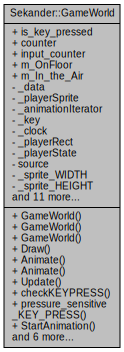
\includegraphics[width=196pt]{classSekander_1_1GameWorld__coll__graph}
\end{center}
\end{figure}
\subsection*{Public Member Functions}
\begin{DoxyCompactItemize}
\item 
\hyperlink{classSekander_1_1GameWorld_a4eba015ae47c7e54c545a874906be1c1}{Game\+World} ()
\item 
\hyperlink{classSekander_1_1GameWorld_a3d57a6627443dcb871f2cc44dd8c5be6}{Game\+World} (\hyperlink{namespaceSekander_a1d69b002ba2d23020901c28f0def5e16}{Game\+Data\+Ref} data)
\item 
\hyperlink{classSekander_1_1GameWorld_a7e626b7986bea0d59a262aac5f47f0cd}{Game\+World} (\hyperlink{namespaceSekander_a1d69b002ba2d23020901c28f0def5e16}{Game\+Data\+Ref} data, std\+::string key, std\+::string file\+\_\+name, int source\+\_\+x, int source\+\_\+y, int sprite\+\_\+\+W\+I\+D\+TH, int sprite\+\_\+\+H\+E\+I\+G\+HT, bool dynamic, int sprite\+\_\+\+X\+\_\+\+F\+R\+A\+M\+ES, int sprite\+\_\+\+Y\+\_\+\+F\+R\+A\+M\+ES, float sprite\+\_\+\+X\+\_\+\+P\+OS, float sprite\+\_\+\+Y\+\_\+\+P\+OS, float sprite\+\_\+\+A\+N\+G\+LE)
\item 
void \hyperlink{classSekander_1_1GameWorld_aefbdb2473bee50c10a5380e7a6892a60}{Draw} ()
\item 
void \hyperlink{classSekander_1_1GameWorld_ad5c3fd7f0c1347d393df075cea46177e}{Animate} (float dt)
\item 
void \hyperlink{classSekander_1_1GameWorld_aa736a4234102bbdbc87dbeb8726d2ce8}{Animate} (float dt, int)
\item 
void \hyperlink{classSekander_1_1GameWorld_a827c7077336d604dd4854196cc6be334}{Update} (float dt)
\item 
const bool \hyperlink{classSekander_1_1GameWorld_a0d0376040dc0171aecdbb5b618741b8b}{check\+K\+E\+Y\+P\+R\+E\+SS} (sf\+::\+Keyboard\+::\+Key)
\item 
bool \hyperlink{classSekander_1_1GameWorld_a543c52aad77747a2f34b5927041ac905}{pressure\+\_\+sensitive\+\_\+\+K\+E\+Y\+\_\+\+P\+R\+E\+SS} (sf\+::\+Keyboard\+::\+Key)
\item 
void \hyperlink{classSekander_1_1GameWorld_a658b6f36a3476b2b8ef0f69a2f0ceac3}{Start\+Animation} ()
\item 
void \hyperlink{classSekander_1_1GameWorld_a1a6c95bf62b4ebb4a9269ebe4ef8ec8b}{Stop\+Animation} ()
\item 
void \hyperlink{classSekander_1_1GameWorld_a38ce97f68d23c6592bc84971db21354f}{Set\+Player\+State} (int player\+State)
\item 
const sf\+::\+Sprite \& \hyperlink{classSekander_1_1GameWorld_ac8b727f77781b0ebeafb3b541bf17a67}{Get\+Sprite} () const
\item 
\hyperlink{namespaceSekander_a1d69b002ba2d23020901c28f0def5e16}{Game\+Data\+Ref} \& \hyperlink{classSekander_1_1GameWorld_aee698ca8d58a687e2321d7524bedabf3}{retrieve\+Data} ()
\item 
void \hyperlink{classSekander_1_1GameWorld_aaa990ab4fb0cc708a7f12ec798ba90ef}{Set\+\_\+\+Y\+\_\+\+Frame} (int change\+\_\+\+Frame)
\item 
sf\+::\+Int\+Rect \hyperlink{classSekander_1_1GameWorld_a060069f1527245efc49cc4bae9306c8d}{return\+\_\+entity\+\_\+rect} ()
\end{DoxyCompactItemize}
\subsection*{Static Public Attributes}
\begin{DoxyCompactItemize}
\item 
static bool \hyperlink{classSekander_1_1GameWorld_a59be267007f51217d7f9739029e966cd}{is\+\_\+key\+\_\+pressed}
\item 
static unsigned short int \hyperlink{classSekander_1_1GameWorld_a8b5e8a9e12e49fcd66361a83837c2b30}{counter}
\item 
static float \hyperlink{classSekander_1_1GameWorld_a0253519bdc4bb36ae9b1c835ecdcedc6}{input\+\_\+counter}
\item 
static bool \hyperlink{classSekander_1_1GameWorld_ad6495d2d0423201c931a147682104417}{m\+\_\+\+On\+Floor} = true
\item 
static bool \hyperlink{classSekander_1_1GameWorld_a2392a1e2b5d6ff4fb352144bf426ae45}{m\+\_\+\+In\+\_\+the\+\_\+\+Air} = false
\end{DoxyCompactItemize}
\subsection*{Private Attributes}
\begin{DoxyCompactItemize}
\item 
\hyperlink{namespaceSekander_a1d69b002ba2d23020901c28f0def5e16}{Game\+Data\+Ref} \hyperlink{classSekander_1_1GameWorld_af884f2489e4a94f95679906932bc0119}{\+\_\+data}
\item 
sf\+::\+Sprite \hyperlink{classSekander_1_1GameWorld_ab15d5f24af33963d1508f31a9b8cb49e}{\+\_\+player\+Sprite}
\item 
unsigned int \hyperlink{classSekander_1_1GameWorld_a5893d4895ff1674d8681216ed8ad7258}{\+\_\+animation\+Iterator}
\item 
std\+::string \hyperlink{classSekander_1_1GameWorld_ace73eff11891a3cbfce71ec1de85f8eb}{\+\_\+key}
\item 
sf\+::\+Clock \hyperlink{classSekander_1_1GameWorld_a825ceb9a0d457b4a8e75d16094ee1c8b}{\+\_\+clock}
\item 
sf\+::\+Int\+Rect \hyperlink{classSekander_1_1GameWorld_abd93d7c6c2b733c5d0a78ea051886fe9}{\+\_\+player\+Rect}
\item 
int \hyperlink{classSekander_1_1GameWorld_a76785ebd5e10d598db14dd1a338172bd}{\+\_\+player\+State}
\item 
sf\+::\+Vector2i \hyperlink{classSekander_1_1GameWorld_a2a23ea4e9dce3bdeee4ce38e2a8a7122}{source}
\item 
int \hyperlink{classSekander_1_1GameWorld_ae71b1a8c967f13881b54f2fee9d3ce3e}{\+\_\+sprite\+\_\+\+W\+I\+D\+TH}
\item 
int \hyperlink{classSekander_1_1GameWorld_af8466397055debb51fbdd1c2808af51f}{\+\_\+sprite\+\_\+\+H\+E\+I\+G\+HT}
\item 
int \hyperlink{classSekander_1_1GameWorld_a7aa72bbfd5f1b4f7ab04c819b815f7be}{\+\_\+sprite\+\_\+\+X\+\_\+\+F\+R\+A\+M\+ES}
\item 
int \hyperlink{classSekander_1_1GameWorld_a55975c2cb042a079708c204ff24695d6}{\+\_\+sprite\+\_\+\+Y\+\_\+\+F\+R\+A\+M\+ES}
\item 
float \hyperlink{classSekander_1_1GameWorld_a3b4e98fc1c72a8d126f58fc1d65267bf}{\+\_\+sprite\+\_\+\+X\+\_\+\+P\+OS}
\item 
float \hyperlink{classSekander_1_1GameWorld_ac9cee04f7adc8cca928b1fb166c2bac5}{\+\_\+sprite\+\_\+\+Y\+\_\+\+P\+OS}
\item 
b2\+Polygon\+Shape $\ast$ \hyperlink{classSekander_1_1GameWorld_a0797c51490bfc5a53b8effac8f195a65}{polygon\+Shape}
\item 
b2\+Edge\+Shape $\ast$ \hyperlink{classSekander_1_1GameWorld_a3efbbb851ccda6cc754ae5a567a6215a}{poly}
\item 
b2\+Body $\ast$ \hyperlink{classSekander_1_1GameWorld_a2ceefac22fc6906e1522abf7ca0be576}{player}
\item 
b2\+Body $\ast$ \hyperlink{classSekander_1_1GameWorld_ad95a5d205f8b25013916ceec88710042}{bullet}
\item 
b2\+Body $\ast$ \hyperlink{classSekander_1_1GameWorld_ae9290e904834fca5fa209a6bddb53bd6}{enemy}
\item 
b2\+Body $\ast$ \hyperlink{classSekander_1_1GameWorld_a9267f9cb0e1678b46196ab8bef1de654}{floor}
\item 
b2\+Body $\ast$ \hyperlink{classSekander_1_1GameWorld_a0a67f9a7d37aa2aaa03e1a66a46119e8}{wall}
\end{DoxyCompactItemize}


\subsection{Constructor \& Destructor Documentation}
\mbox{\Hypertarget{classSekander_1_1GameWorld_a4eba015ae47c7e54c545a874906be1c1}\label{classSekander_1_1GameWorld_a4eba015ae47c7e54c545a874906be1c1}} 
\index{Sekander\+::\+Game\+World@{Sekander\+::\+Game\+World}!Game\+World@{Game\+World}}
\index{Game\+World@{Game\+World}!Sekander\+::\+Game\+World@{Sekander\+::\+Game\+World}}
\subsubsection{\texorpdfstring{Game\+World()}{GameWorld()}\hspace{0.1cm}{\footnotesize\ttfamily [1/3]}}
{\footnotesize\ttfamily Sekander\+::\+Game\+World\+::\+Game\+World (\begin{DoxyParamCaption}{ }\end{DoxyParamCaption})}

\mbox{\Hypertarget{classSekander_1_1GameWorld_a3d57a6627443dcb871f2cc44dd8c5be6}\label{classSekander_1_1GameWorld_a3d57a6627443dcb871f2cc44dd8c5be6}} 
\index{Sekander\+::\+Game\+World@{Sekander\+::\+Game\+World}!Game\+World@{Game\+World}}
\index{Game\+World@{Game\+World}!Sekander\+::\+Game\+World@{Sekander\+::\+Game\+World}}
\subsubsection{\texorpdfstring{Game\+World()}{GameWorld()}\hspace{0.1cm}{\footnotesize\ttfamily [2/3]}}
{\footnotesize\ttfamily Sekander\+::\+Game\+World\+::\+Game\+World (\begin{DoxyParamCaption}\item[{\hyperlink{namespaceSekander_a1d69b002ba2d23020901c28f0def5e16}{Game\+Data\+Ref}}]{data }\end{DoxyParamCaption})}

\mbox{\Hypertarget{classSekander_1_1GameWorld_a7e626b7986bea0d59a262aac5f47f0cd}\label{classSekander_1_1GameWorld_a7e626b7986bea0d59a262aac5f47f0cd}} 
\index{Sekander\+::\+Game\+World@{Sekander\+::\+Game\+World}!Game\+World@{Game\+World}}
\index{Game\+World@{Game\+World}!Sekander\+::\+Game\+World@{Sekander\+::\+Game\+World}}
\subsubsection{\texorpdfstring{Game\+World()}{GameWorld()}\hspace{0.1cm}{\footnotesize\ttfamily [3/3]}}
{\footnotesize\ttfamily Sekander\+::\+Game\+World\+::\+Game\+World (\begin{DoxyParamCaption}\item[{\hyperlink{namespaceSekander_a1d69b002ba2d23020901c28f0def5e16}{Game\+Data\+Ref}}]{data,  }\item[{std\+::string}]{key,  }\item[{std\+::string}]{file\+\_\+name,  }\item[{int}]{source\+\_\+x,  }\item[{int}]{source\+\_\+y,  }\item[{int}]{sprite\+\_\+\+W\+I\+D\+TH,  }\item[{int}]{sprite\+\_\+\+H\+E\+I\+G\+HT,  }\item[{bool}]{dynamic,  }\item[{int}]{sprite\+\_\+\+X\+\_\+\+F\+R\+A\+M\+ES,  }\item[{int}]{sprite\+\_\+\+Y\+\_\+\+F\+R\+A\+M\+ES,  }\item[{float}]{sprite\+\_\+\+X\+\_\+\+P\+OS,  }\item[{float}]{sprite\+\_\+\+Y\+\_\+\+P\+OS,  }\item[{float}]{sprite\+\_\+\+A\+N\+G\+LE }\end{DoxyParamCaption})\hspace{0.3cm}{\ttfamily [explicit]}}



\subsection{Member Function Documentation}
\mbox{\Hypertarget{classSekander_1_1GameWorld_ad5c3fd7f0c1347d393df075cea46177e}\label{classSekander_1_1GameWorld_ad5c3fd7f0c1347d393df075cea46177e}} 
\index{Sekander\+::\+Game\+World@{Sekander\+::\+Game\+World}!Animate@{Animate}}
\index{Animate@{Animate}!Sekander\+::\+Game\+World@{Sekander\+::\+Game\+World}}
\subsubsection{\texorpdfstring{Animate()}{Animate()}\hspace{0.1cm}{\footnotesize\ttfamily [1/2]}}
{\footnotesize\ttfamily void Sekander\+::\+Game\+World\+::\+Animate (\begin{DoxyParamCaption}\item[{float}]{dt }\end{DoxyParamCaption})}

\mbox{\Hypertarget{classSekander_1_1GameWorld_aa736a4234102bbdbc87dbeb8726d2ce8}\label{classSekander_1_1GameWorld_aa736a4234102bbdbc87dbeb8726d2ce8}} 
\index{Sekander\+::\+Game\+World@{Sekander\+::\+Game\+World}!Animate@{Animate}}
\index{Animate@{Animate}!Sekander\+::\+Game\+World@{Sekander\+::\+Game\+World}}
\subsubsection{\texorpdfstring{Animate()}{Animate()}\hspace{0.1cm}{\footnotesize\ttfamily [2/2]}}
{\footnotesize\ttfamily void Sekander\+::\+Game\+World\+::\+Animate (\begin{DoxyParamCaption}\item[{float}]{dt,  }\item[{int}]{Y\+\_\+\+F\+R\+A\+ME }\end{DoxyParamCaption})}

\mbox{\Hypertarget{classSekander_1_1GameWorld_a0d0376040dc0171aecdbb5b618741b8b}\label{classSekander_1_1GameWorld_a0d0376040dc0171aecdbb5b618741b8b}} 
\index{Sekander\+::\+Game\+World@{Sekander\+::\+Game\+World}!check\+K\+E\+Y\+P\+R\+E\+SS@{check\+K\+E\+Y\+P\+R\+E\+SS}}
\index{check\+K\+E\+Y\+P\+R\+E\+SS@{check\+K\+E\+Y\+P\+R\+E\+SS}!Sekander\+::\+Game\+World@{Sekander\+::\+Game\+World}}
\subsubsection{\texorpdfstring{check\+K\+E\+Y\+P\+R\+E\+S\+S()}{checkKEYPRESS()}}
{\footnotesize\ttfamily const bool Sekander\+::\+Game\+World\+::check\+K\+E\+Y\+P\+R\+E\+SS (\begin{DoxyParamCaption}\item[{sf\+::\+Keyboard\+::\+Key}]{key }\end{DoxyParamCaption})}

\mbox{\Hypertarget{classSekander_1_1GameWorld_aefbdb2473bee50c10a5380e7a6892a60}\label{classSekander_1_1GameWorld_aefbdb2473bee50c10a5380e7a6892a60}} 
\index{Sekander\+::\+Game\+World@{Sekander\+::\+Game\+World}!Draw@{Draw}}
\index{Draw@{Draw}!Sekander\+::\+Game\+World@{Sekander\+::\+Game\+World}}
\subsubsection{\texorpdfstring{Draw()}{Draw()}}
{\footnotesize\ttfamily void Sekander\+::\+Game\+World\+::\+Draw (\begin{DoxyParamCaption}{ }\end{DoxyParamCaption})}

\mbox{\Hypertarget{classSekander_1_1GameWorld_ac8b727f77781b0ebeafb3b541bf17a67}\label{classSekander_1_1GameWorld_ac8b727f77781b0ebeafb3b541bf17a67}} 
\index{Sekander\+::\+Game\+World@{Sekander\+::\+Game\+World}!Get\+Sprite@{Get\+Sprite}}
\index{Get\+Sprite@{Get\+Sprite}!Sekander\+::\+Game\+World@{Sekander\+::\+Game\+World}}
\subsubsection{\texorpdfstring{Get\+Sprite()}{GetSprite()}}
{\footnotesize\ttfamily const sf\+::\+Sprite \& Sekander\+::\+Game\+World\+::\+Get\+Sprite (\begin{DoxyParamCaption}{ }\end{DoxyParamCaption}) const}

\mbox{\Hypertarget{classSekander_1_1GameWorld_a543c52aad77747a2f34b5927041ac905}\label{classSekander_1_1GameWorld_a543c52aad77747a2f34b5927041ac905}} 
\index{Sekander\+::\+Game\+World@{Sekander\+::\+Game\+World}!pressure\+\_\+sensitive\+\_\+\+K\+E\+Y\+\_\+\+P\+R\+E\+SS@{pressure\+\_\+sensitive\+\_\+\+K\+E\+Y\+\_\+\+P\+R\+E\+SS}}
\index{pressure\+\_\+sensitive\+\_\+\+K\+E\+Y\+\_\+\+P\+R\+E\+SS@{pressure\+\_\+sensitive\+\_\+\+K\+E\+Y\+\_\+\+P\+R\+E\+SS}!Sekander\+::\+Game\+World@{Sekander\+::\+Game\+World}}
\subsubsection{\texorpdfstring{pressure\+\_\+sensitive\+\_\+\+K\+E\+Y\+\_\+\+P\+R\+E\+S\+S()}{pressure\_sensitive\_KEY\_PRESS()}}
{\footnotesize\ttfamily bool Sekander\+::\+Game\+World\+::pressure\+\_\+sensitive\+\_\+\+K\+E\+Y\+\_\+\+P\+R\+E\+SS (\begin{DoxyParamCaption}\item[{sf\+::\+Keyboard\+::\+Key}]{key }\end{DoxyParamCaption})}

\mbox{\Hypertarget{classSekander_1_1GameWorld_aee698ca8d58a687e2321d7524bedabf3}\label{classSekander_1_1GameWorld_aee698ca8d58a687e2321d7524bedabf3}} 
\index{Sekander\+::\+Game\+World@{Sekander\+::\+Game\+World}!retrieve\+Data@{retrieve\+Data}}
\index{retrieve\+Data@{retrieve\+Data}!Sekander\+::\+Game\+World@{Sekander\+::\+Game\+World}}
\subsubsection{\texorpdfstring{retrieve\+Data()}{retrieveData()}}
{\footnotesize\ttfamily \hyperlink{namespaceSekander_a1d69b002ba2d23020901c28f0def5e16}{Game\+Data\+Ref}\& Sekander\+::\+Game\+World\+::retrieve\+Data (\begin{DoxyParamCaption}{ }\end{DoxyParamCaption})\hspace{0.3cm}{\ttfamily [inline]}}

\mbox{\Hypertarget{classSekander_1_1GameWorld_a060069f1527245efc49cc4bae9306c8d}\label{classSekander_1_1GameWorld_a060069f1527245efc49cc4bae9306c8d}} 
\index{Sekander\+::\+Game\+World@{Sekander\+::\+Game\+World}!return\+\_\+entity\+\_\+rect@{return\+\_\+entity\+\_\+rect}}
\index{return\+\_\+entity\+\_\+rect@{return\+\_\+entity\+\_\+rect}!Sekander\+::\+Game\+World@{Sekander\+::\+Game\+World}}
\subsubsection{\texorpdfstring{return\+\_\+entity\+\_\+rect()}{return\_entity\_rect()}}
{\footnotesize\ttfamily sf\+::\+Int\+Rect Sekander\+::\+Game\+World\+::return\+\_\+entity\+\_\+rect (\begin{DoxyParamCaption}{ }\end{DoxyParamCaption})\hspace{0.3cm}{\ttfamily [inline]}}

\mbox{\Hypertarget{classSekander_1_1GameWorld_aaa990ab4fb0cc708a7f12ec798ba90ef}\label{classSekander_1_1GameWorld_aaa990ab4fb0cc708a7f12ec798ba90ef}} 
\index{Sekander\+::\+Game\+World@{Sekander\+::\+Game\+World}!Set\+\_\+\+Y\+\_\+\+Frame@{Set\+\_\+\+Y\+\_\+\+Frame}}
\index{Set\+\_\+\+Y\+\_\+\+Frame@{Set\+\_\+\+Y\+\_\+\+Frame}!Sekander\+::\+Game\+World@{Sekander\+::\+Game\+World}}
\subsubsection{\texorpdfstring{Set\+\_\+\+Y\+\_\+\+Frame()}{Set\_Y\_Frame()}}
{\footnotesize\ttfamily void Sekander\+::\+Game\+World\+::\+Set\+\_\+\+Y\+\_\+\+Frame (\begin{DoxyParamCaption}\item[{int}]{change\+\_\+\+Frame }\end{DoxyParamCaption})\hspace{0.3cm}{\ttfamily [inline]}}

\mbox{\Hypertarget{classSekander_1_1GameWorld_a38ce97f68d23c6592bc84971db21354f}\label{classSekander_1_1GameWorld_a38ce97f68d23c6592bc84971db21354f}} 
\index{Sekander\+::\+Game\+World@{Sekander\+::\+Game\+World}!Set\+Player\+State@{Set\+Player\+State}}
\index{Set\+Player\+State@{Set\+Player\+State}!Sekander\+::\+Game\+World@{Sekander\+::\+Game\+World}}
\subsubsection{\texorpdfstring{Set\+Player\+State()}{SetPlayerState()}}
{\footnotesize\ttfamily void Sekander\+::\+Game\+World\+::\+Set\+Player\+State (\begin{DoxyParamCaption}\item[{int}]{player\+State }\end{DoxyParamCaption})\hspace{0.3cm}{\ttfamily [inline]}}

\mbox{\Hypertarget{classSekander_1_1GameWorld_a658b6f36a3476b2b8ef0f69a2f0ceac3}\label{classSekander_1_1GameWorld_a658b6f36a3476b2b8ef0f69a2f0ceac3}} 
\index{Sekander\+::\+Game\+World@{Sekander\+::\+Game\+World}!Start\+Animation@{Start\+Animation}}
\index{Start\+Animation@{Start\+Animation}!Sekander\+::\+Game\+World@{Sekander\+::\+Game\+World}}
\subsubsection{\texorpdfstring{Start\+Animation()}{StartAnimation()}}
{\footnotesize\ttfamily void Sekander\+::\+Game\+World\+::\+Start\+Animation (\begin{DoxyParamCaption}{ }\end{DoxyParamCaption})\hspace{0.3cm}{\ttfamily [inline]}}

\mbox{\Hypertarget{classSekander_1_1GameWorld_a1a6c95bf62b4ebb4a9269ebe4ef8ec8b}\label{classSekander_1_1GameWorld_a1a6c95bf62b4ebb4a9269ebe4ef8ec8b}} 
\index{Sekander\+::\+Game\+World@{Sekander\+::\+Game\+World}!Stop\+Animation@{Stop\+Animation}}
\index{Stop\+Animation@{Stop\+Animation}!Sekander\+::\+Game\+World@{Sekander\+::\+Game\+World}}
\subsubsection{\texorpdfstring{Stop\+Animation()}{StopAnimation()}}
{\footnotesize\ttfamily void Sekander\+::\+Game\+World\+::\+Stop\+Animation (\begin{DoxyParamCaption}{ }\end{DoxyParamCaption})\hspace{0.3cm}{\ttfamily [inline]}}

\mbox{\Hypertarget{classSekander_1_1GameWorld_a827c7077336d604dd4854196cc6be334}\label{classSekander_1_1GameWorld_a827c7077336d604dd4854196cc6be334}} 
\index{Sekander\+::\+Game\+World@{Sekander\+::\+Game\+World}!Update@{Update}}
\index{Update@{Update}!Sekander\+::\+Game\+World@{Sekander\+::\+Game\+World}}
\subsubsection{\texorpdfstring{Update()}{Update()}}
{\footnotesize\ttfamily void Sekander\+::\+Game\+World\+::\+Update (\begin{DoxyParamCaption}\item[{float}]{dt }\end{DoxyParamCaption})}



\subsection{Member Data Documentation}
\mbox{\Hypertarget{classSekander_1_1GameWorld_a5893d4895ff1674d8681216ed8ad7258}\label{classSekander_1_1GameWorld_a5893d4895ff1674d8681216ed8ad7258}} 
\index{Sekander\+::\+Game\+World@{Sekander\+::\+Game\+World}!\+\_\+animation\+Iterator@{\+\_\+animation\+Iterator}}
\index{\+\_\+animation\+Iterator@{\+\_\+animation\+Iterator}!Sekander\+::\+Game\+World@{Sekander\+::\+Game\+World}}
\subsubsection{\texorpdfstring{\+\_\+animation\+Iterator}{\_animationIterator}}
{\footnotesize\ttfamily unsigned int Sekander\+::\+Game\+World\+::\+\_\+animation\+Iterator\hspace{0.3cm}{\ttfamily [private]}}

\mbox{\Hypertarget{classSekander_1_1GameWorld_a825ceb9a0d457b4a8e75d16094ee1c8b}\label{classSekander_1_1GameWorld_a825ceb9a0d457b4a8e75d16094ee1c8b}} 
\index{Sekander\+::\+Game\+World@{Sekander\+::\+Game\+World}!\+\_\+clock@{\+\_\+clock}}
\index{\+\_\+clock@{\+\_\+clock}!Sekander\+::\+Game\+World@{Sekander\+::\+Game\+World}}
\subsubsection{\texorpdfstring{\+\_\+clock}{\_clock}}
{\footnotesize\ttfamily sf\+::\+Clock Sekander\+::\+Game\+World\+::\+\_\+clock\hspace{0.3cm}{\ttfamily [private]}}

\mbox{\Hypertarget{classSekander_1_1GameWorld_af884f2489e4a94f95679906932bc0119}\label{classSekander_1_1GameWorld_af884f2489e4a94f95679906932bc0119}} 
\index{Sekander\+::\+Game\+World@{Sekander\+::\+Game\+World}!\+\_\+data@{\+\_\+data}}
\index{\+\_\+data@{\+\_\+data}!Sekander\+::\+Game\+World@{Sekander\+::\+Game\+World}}
\subsubsection{\texorpdfstring{\+\_\+data}{\_data}}
{\footnotesize\ttfamily \hyperlink{namespaceSekander_a1d69b002ba2d23020901c28f0def5e16}{Game\+Data\+Ref} Sekander\+::\+Game\+World\+::\+\_\+data\hspace{0.3cm}{\ttfamily [private]}}

\mbox{\Hypertarget{classSekander_1_1GameWorld_ace73eff11891a3cbfce71ec1de85f8eb}\label{classSekander_1_1GameWorld_ace73eff11891a3cbfce71ec1de85f8eb}} 
\index{Sekander\+::\+Game\+World@{Sekander\+::\+Game\+World}!\+\_\+key@{\+\_\+key}}
\index{\+\_\+key@{\+\_\+key}!Sekander\+::\+Game\+World@{Sekander\+::\+Game\+World}}
\subsubsection{\texorpdfstring{\+\_\+key}{\_key}}
{\footnotesize\ttfamily std\+::string Sekander\+::\+Game\+World\+::\+\_\+key\hspace{0.3cm}{\ttfamily [private]}}

\mbox{\Hypertarget{classSekander_1_1GameWorld_abd93d7c6c2b733c5d0a78ea051886fe9}\label{classSekander_1_1GameWorld_abd93d7c6c2b733c5d0a78ea051886fe9}} 
\index{Sekander\+::\+Game\+World@{Sekander\+::\+Game\+World}!\+\_\+player\+Rect@{\+\_\+player\+Rect}}
\index{\+\_\+player\+Rect@{\+\_\+player\+Rect}!Sekander\+::\+Game\+World@{Sekander\+::\+Game\+World}}
\subsubsection{\texorpdfstring{\+\_\+player\+Rect}{\_playerRect}}
{\footnotesize\ttfamily sf\+::\+Int\+Rect Sekander\+::\+Game\+World\+::\+\_\+player\+Rect\hspace{0.3cm}{\ttfamily [private]}}

\mbox{\Hypertarget{classSekander_1_1GameWorld_ab15d5f24af33963d1508f31a9b8cb49e}\label{classSekander_1_1GameWorld_ab15d5f24af33963d1508f31a9b8cb49e}} 
\index{Sekander\+::\+Game\+World@{Sekander\+::\+Game\+World}!\+\_\+player\+Sprite@{\+\_\+player\+Sprite}}
\index{\+\_\+player\+Sprite@{\+\_\+player\+Sprite}!Sekander\+::\+Game\+World@{Sekander\+::\+Game\+World}}
\subsubsection{\texorpdfstring{\+\_\+player\+Sprite}{\_playerSprite}}
{\footnotesize\ttfamily sf\+::\+Sprite Sekander\+::\+Game\+World\+::\+\_\+player\+Sprite\hspace{0.3cm}{\ttfamily [private]}}

\mbox{\Hypertarget{classSekander_1_1GameWorld_a76785ebd5e10d598db14dd1a338172bd}\label{classSekander_1_1GameWorld_a76785ebd5e10d598db14dd1a338172bd}} 
\index{Sekander\+::\+Game\+World@{Sekander\+::\+Game\+World}!\+\_\+player\+State@{\+\_\+player\+State}}
\index{\+\_\+player\+State@{\+\_\+player\+State}!Sekander\+::\+Game\+World@{Sekander\+::\+Game\+World}}
\subsubsection{\texorpdfstring{\+\_\+player\+State}{\_playerState}}
{\footnotesize\ttfamily int Sekander\+::\+Game\+World\+::\+\_\+player\+State\hspace{0.3cm}{\ttfamily [private]}}

\mbox{\Hypertarget{classSekander_1_1GameWorld_af8466397055debb51fbdd1c2808af51f}\label{classSekander_1_1GameWorld_af8466397055debb51fbdd1c2808af51f}} 
\index{Sekander\+::\+Game\+World@{Sekander\+::\+Game\+World}!\+\_\+sprite\+\_\+\+H\+E\+I\+G\+HT@{\+\_\+sprite\+\_\+\+H\+E\+I\+G\+HT}}
\index{\+\_\+sprite\+\_\+\+H\+E\+I\+G\+HT@{\+\_\+sprite\+\_\+\+H\+E\+I\+G\+HT}!Sekander\+::\+Game\+World@{Sekander\+::\+Game\+World}}
\subsubsection{\texorpdfstring{\+\_\+sprite\+\_\+\+H\+E\+I\+G\+HT}{\_sprite\_HEIGHT}}
{\footnotesize\ttfamily int Sekander\+::\+Game\+World\+::\+\_\+sprite\+\_\+\+H\+E\+I\+G\+HT\hspace{0.3cm}{\ttfamily [private]}}

\mbox{\Hypertarget{classSekander_1_1GameWorld_ae71b1a8c967f13881b54f2fee9d3ce3e}\label{classSekander_1_1GameWorld_ae71b1a8c967f13881b54f2fee9d3ce3e}} 
\index{Sekander\+::\+Game\+World@{Sekander\+::\+Game\+World}!\+\_\+sprite\+\_\+\+W\+I\+D\+TH@{\+\_\+sprite\+\_\+\+W\+I\+D\+TH}}
\index{\+\_\+sprite\+\_\+\+W\+I\+D\+TH@{\+\_\+sprite\+\_\+\+W\+I\+D\+TH}!Sekander\+::\+Game\+World@{Sekander\+::\+Game\+World}}
\subsubsection{\texorpdfstring{\+\_\+sprite\+\_\+\+W\+I\+D\+TH}{\_sprite\_WIDTH}}
{\footnotesize\ttfamily int Sekander\+::\+Game\+World\+::\+\_\+sprite\+\_\+\+W\+I\+D\+TH\hspace{0.3cm}{\ttfamily [private]}}

\mbox{\Hypertarget{classSekander_1_1GameWorld_a7aa72bbfd5f1b4f7ab04c819b815f7be}\label{classSekander_1_1GameWorld_a7aa72bbfd5f1b4f7ab04c819b815f7be}} 
\index{Sekander\+::\+Game\+World@{Sekander\+::\+Game\+World}!\+\_\+sprite\+\_\+\+X\+\_\+\+F\+R\+A\+M\+ES@{\+\_\+sprite\+\_\+\+X\+\_\+\+F\+R\+A\+M\+ES}}
\index{\+\_\+sprite\+\_\+\+X\+\_\+\+F\+R\+A\+M\+ES@{\+\_\+sprite\+\_\+\+X\+\_\+\+F\+R\+A\+M\+ES}!Sekander\+::\+Game\+World@{Sekander\+::\+Game\+World}}
\subsubsection{\texorpdfstring{\+\_\+sprite\+\_\+\+X\+\_\+\+F\+R\+A\+M\+ES}{\_sprite\_X\_FRAMES}}
{\footnotesize\ttfamily int Sekander\+::\+Game\+World\+::\+\_\+sprite\+\_\+\+X\+\_\+\+F\+R\+A\+M\+ES\hspace{0.3cm}{\ttfamily [private]}}

\mbox{\Hypertarget{classSekander_1_1GameWorld_a3b4e98fc1c72a8d126f58fc1d65267bf}\label{classSekander_1_1GameWorld_a3b4e98fc1c72a8d126f58fc1d65267bf}} 
\index{Sekander\+::\+Game\+World@{Sekander\+::\+Game\+World}!\+\_\+sprite\+\_\+\+X\+\_\+\+P\+OS@{\+\_\+sprite\+\_\+\+X\+\_\+\+P\+OS}}
\index{\+\_\+sprite\+\_\+\+X\+\_\+\+P\+OS@{\+\_\+sprite\+\_\+\+X\+\_\+\+P\+OS}!Sekander\+::\+Game\+World@{Sekander\+::\+Game\+World}}
\subsubsection{\texorpdfstring{\+\_\+sprite\+\_\+\+X\+\_\+\+P\+OS}{\_sprite\_X\_POS}}
{\footnotesize\ttfamily float Sekander\+::\+Game\+World\+::\+\_\+sprite\+\_\+\+X\+\_\+\+P\+OS\hspace{0.3cm}{\ttfamily [private]}}

\mbox{\Hypertarget{classSekander_1_1GameWorld_a55975c2cb042a079708c204ff24695d6}\label{classSekander_1_1GameWorld_a55975c2cb042a079708c204ff24695d6}} 
\index{Sekander\+::\+Game\+World@{Sekander\+::\+Game\+World}!\+\_\+sprite\+\_\+\+Y\+\_\+\+F\+R\+A\+M\+ES@{\+\_\+sprite\+\_\+\+Y\+\_\+\+F\+R\+A\+M\+ES}}
\index{\+\_\+sprite\+\_\+\+Y\+\_\+\+F\+R\+A\+M\+ES@{\+\_\+sprite\+\_\+\+Y\+\_\+\+F\+R\+A\+M\+ES}!Sekander\+::\+Game\+World@{Sekander\+::\+Game\+World}}
\subsubsection{\texorpdfstring{\+\_\+sprite\+\_\+\+Y\+\_\+\+F\+R\+A\+M\+ES}{\_sprite\_Y\_FRAMES}}
{\footnotesize\ttfamily int Sekander\+::\+Game\+World\+::\+\_\+sprite\+\_\+\+Y\+\_\+\+F\+R\+A\+M\+ES\hspace{0.3cm}{\ttfamily [private]}}

\mbox{\Hypertarget{classSekander_1_1GameWorld_ac9cee04f7adc8cca928b1fb166c2bac5}\label{classSekander_1_1GameWorld_ac9cee04f7adc8cca928b1fb166c2bac5}} 
\index{Sekander\+::\+Game\+World@{Sekander\+::\+Game\+World}!\+\_\+sprite\+\_\+\+Y\+\_\+\+P\+OS@{\+\_\+sprite\+\_\+\+Y\+\_\+\+P\+OS}}
\index{\+\_\+sprite\+\_\+\+Y\+\_\+\+P\+OS@{\+\_\+sprite\+\_\+\+Y\+\_\+\+P\+OS}!Sekander\+::\+Game\+World@{Sekander\+::\+Game\+World}}
\subsubsection{\texorpdfstring{\+\_\+sprite\+\_\+\+Y\+\_\+\+P\+OS}{\_sprite\_Y\_POS}}
{\footnotesize\ttfamily float Sekander\+::\+Game\+World\+::\+\_\+sprite\+\_\+\+Y\+\_\+\+P\+OS\hspace{0.3cm}{\ttfamily [private]}}

\mbox{\Hypertarget{classSekander_1_1GameWorld_ad95a5d205f8b25013916ceec88710042}\label{classSekander_1_1GameWorld_ad95a5d205f8b25013916ceec88710042}} 
\index{Sekander\+::\+Game\+World@{Sekander\+::\+Game\+World}!bullet@{bullet}}
\index{bullet@{bullet}!Sekander\+::\+Game\+World@{Sekander\+::\+Game\+World}}
\subsubsection{\texorpdfstring{bullet}{bullet}}
{\footnotesize\ttfamily b2\+Body$\ast$ Sekander\+::\+Game\+World\+::bullet\hspace{0.3cm}{\ttfamily [private]}}

\mbox{\Hypertarget{classSekander_1_1GameWorld_a8b5e8a9e12e49fcd66361a83837c2b30}\label{classSekander_1_1GameWorld_a8b5e8a9e12e49fcd66361a83837c2b30}} 
\index{Sekander\+::\+Game\+World@{Sekander\+::\+Game\+World}!counter@{counter}}
\index{counter@{counter}!Sekander\+::\+Game\+World@{Sekander\+::\+Game\+World}}
\subsubsection{\texorpdfstring{counter}{counter}}
{\footnotesize\ttfamily unsigned short int Sekander\+::\+Game\+World\+::counter\hspace{0.3cm}{\ttfamily [inline]}, {\ttfamily [static]}}

\mbox{\Hypertarget{classSekander_1_1GameWorld_ae9290e904834fca5fa209a6bddb53bd6}\label{classSekander_1_1GameWorld_ae9290e904834fca5fa209a6bddb53bd6}} 
\index{Sekander\+::\+Game\+World@{Sekander\+::\+Game\+World}!enemy@{enemy}}
\index{enemy@{enemy}!Sekander\+::\+Game\+World@{Sekander\+::\+Game\+World}}
\subsubsection{\texorpdfstring{enemy}{enemy}}
{\footnotesize\ttfamily b2\+Body$\ast$ Sekander\+::\+Game\+World\+::enemy\hspace{0.3cm}{\ttfamily [private]}}

\mbox{\Hypertarget{classSekander_1_1GameWorld_a9267f9cb0e1678b46196ab8bef1de654}\label{classSekander_1_1GameWorld_a9267f9cb0e1678b46196ab8bef1de654}} 
\index{Sekander\+::\+Game\+World@{Sekander\+::\+Game\+World}!floor@{floor}}
\index{floor@{floor}!Sekander\+::\+Game\+World@{Sekander\+::\+Game\+World}}
\subsubsection{\texorpdfstring{floor}{floor}}
{\footnotesize\ttfamily b2\+Body$\ast$ Sekander\+::\+Game\+World\+::floor\hspace{0.3cm}{\ttfamily [private]}}

\mbox{\Hypertarget{classSekander_1_1GameWorld_a0253519bdc4bb36ae9b1c835ecdcedc6}\label{classSekander_1_1GameWorld_a0253519bdc4bb36ae9b1c835ecdcedc6}} 
\index{Sekander\+::\+Game\+World@{Sekander\+::\+Game\+World}!input\+\_\+counter@{input\+\_\+counter}}
\index{input\+\_\+counter@{input\+\_\+counter}!Sekander\+::\+Game\+World@{Sekander\+::\+Game\+World}}
\subsubsection{\texorpdfstring{input\+\_\+counter}{input\_counter}}
{\footnotesize\ttfamily float Sekander\+::\+Game\+World\+::input\+\_\+counter\hspace{0.3cm}{\ttfamily [inline]}, {\ttfamily [static]}}

\mbox{\Hypertarget{classSekander_1_1GameWorld_a59be267007f51217d7f9739029e966cd}\label{classSekander_1_1GameWorld_a59be267007f51217d7f9739029e966cd}} 
\index{Sekander\+::\+Game\+World@{Sekander\+::\+Game\+World}!is\+\_\+key\+\_\+pressed@{is\+\_\+key\+\_\+pressed}}
\index{is\+\_\+key\+\_\+pressed@{is\+\_\+key\+\_\+pressed}!Sekander\+::\+Game\+World@{Sekander\+::\+Game\+World}}
\subsubsection{\texorpdfstring{is\+\_\+key\+\_\+pressed}{is\_key\_pressed}}
{\footnotesize\ttfamily bool Sekander\+::\+Game\+World\+::is\+\_\+key\+\_\+pressed\hspace{0.3cm}{\ttfamily [inline]}, {\ttfamily [static]}}

\mbox{\Hypertarget{classSekander_1_1GameWorld_a2392a1e2b5d6ff4fb352144bf426ae45}\label{classSekander_1_1GameWorld_a2392a1e2b5d6ff4fb352144bf426ae45}} 
\index{Sekander\+::\+Game\+World@{Sekander\+::\+Game\+World}!m\+\_\+\+In\+\_\+the\+\_\+\+Air@{m\+\_\+\+In\+\_\+the\+\_\+\+Air}}
\index{m\+\_\+\+In\+\_\+the\+\_\+\+Air@{m\+\_\+\+In\+\_\+the\+\_\+\+Air}!Sekander\+::\+Game\+World@{Sekander\+::\+Game\+World}}
\subsubsection{\texorpdfstring{m\+\_\+\+In\+\_\+the\+\_\+\+Air}{m\_In\_the\_Air}}
{\footnotesize\ttfamily bool Sekander\+::\+Game\+World\+::m\+\_\+\+In\+\_\+the\+\_\+\+Air = false\hspace{0.3cm}{\ttfamily [inline]}, {\ttfamily [static]}}

\mbox{\Hypertarget{classSekander_1_1GameWorld_ad6495d2d0423201c931a147682104417}\label{classSekander_1_1GameWorld_ad6495d2d0423201c931a147682104417}} 
\index{Sekander\+::\+Game\+World@{Sekander\+::\+Game\+World}!m\+\_\+\+On\+Floor@{m\+\_\+\+On\+Floor}}
\index{m\+\_\+\+On\+Floor@{m\+\_\+\+On\+Floor}!Sekander\+::\+Game\+World@{Sekander\+::\+Game\+World}}
\subsubsection{\texorpdfstring{m\+\_\+\+On\+Floor}{m\_OnFloor}}
{\footnotesize\ttfamily bool Sekander\+::\+Game\+World\+::m\+\_\+\+On\+Floor = true\hspace{0.3cm}{\ttfamily [inline]}, {\ttfamily [static]}}

\mbox{\Hypertarget{classSekander_1_1GameWorld_a2ceefac22fc6906e1522abf7ca0be576}\label{classSekander_1_1GameWorld_a2ceefac22fc6906e1522abf7ca0be576}} 
\index{Sekander\+::\+Game\+World@{Sekander\+::\+Game\+World}!player@{player}}
\index{player@{player}!Sekander\+::\+Game\+World@{Sekander\+::\+Game\+World}}
\subsubsection{\texorpdfstring{player}{player}}
{\footnotesize\ttfamily b2\+Body$\ast$ Sekander\+::\+Game\+World\+::player\hspace{0.3cm}{\ttfamily [private]}}

\mbox{\Hypertarget{classSekander_1_1GameWorld_a3efbbb851ccda6cc754ae5a567a6215a}\label{classSekander_1_1GameWorld_a3efbbb851ccda6cc754ae5a567a6215a}} 
\index{Sekander\+::\+Game\+World@{Sekander\+::\+Game\+World}!poly@{poly}}
\index{poly@{poly}!Sekander\+::\+Game\+World@{Sekander\+::\+Game\+World}}
\subsubsection{\texorpdfstring{poly}{poly}}
{\footnotesize\ttfamily b2\+Edge\+Shape$\ast$ Sekander\+::\+Game\+World\+::poly\hspace{0.3cm}{\ttfamily [private]}}

\mbox{\Hypertarget{classSekander_1_1GameWorld_a0797c51490bfc5a53b8effac8f195a65}\label{classSekander_1_1GameWorld_a0797c51490bfc5a53b8effac8f195a65}} 
\index{Sekander\+::\+Game\+World@{Sekander\+::\+Game\+World}!polygon\+Shape@{polygon\+Shape}}
\index{polygon\+Shape@{polygon\+Shape}!Sekander\+::\+Game\+World@{Sekander\+::\+Game\+World}}
\subsubsection{\texorpdfstring{polygon\+Shape}{polygonShape}}
{\footnotesize\ttfamily b2\+Polygon\+Shape$\ast$ Sekander\+::\+Game\+World\+::polygon\+Shape\hspace{0.3cm}{\ttfamily [private]}}

\mbox{\Hypertarget{classSekander_1_1GameWorld_a2a23ea4e9dce3bdeee4ce38e2a8a7122}\label{classSekander_1_1GameWorld_a2a23ea4e9dce3bdeee4ce38e2a8a7122}} 
\index{Sekander\+::\+Game\+World@{Sekander\+::\+Game\+World}!source@{source}}
\index{source@{source}!Sekander\+::\+Game\+World@{Sekander\+::\+Game\+World}}
\subsubsection{\texorpdfstring{source}{source}}
{\footnotesize\ttfamily sf\+::\+Vector2i Sekander\+::\+Game\+World\+::source\hspace{0.3cm}{\ttfamily [private]}}

\mbox{\Hypertarget{classSekander_1_1GameWorld_a0a67f9a7d37aa2aaa03e1a66a46119e8}\label{classSekander_1_1GameWorld_a0a67f9a7d37aa2aaa03e1a66a46119e8}} 
\index{Sekander\+::\+Game\+World@{Sekander\+::\+Game\+World}!wall@{wall}}
\index{wall@{wall}!Sekander\+::\+Game\+World@{Sekander\+::\+Game\+World}}
\subsubsection{\texorpdfstring{wall}{wall}}
{\footnotesize\ttfamily b2\+Body$\ast$ Sekander\+::\+Game\+World\+::wall\hspace{0.3cm}{\ttfamily [private]}}



The documentation for this class was generated from the following files\+:\begin{DoxyCompactItemize}
\item 
/mnt/hdd/\+C0de/\+Engines/\+S\+F\+M\+L/\+S\+F\+M\+L\+\_\+\+Engine/include/\hyperlink{GameWorld_8hpp}{Game\+World.\+hpp}\item 
/mnt/hdd/\+C0de/\+Engines/\+S\+F\+M\+L/\+S\+F\+M\+L\+\_\+\+Engine/src/\hyperlink{GameWorld_8cpp}{Game\+World.\+cpp}\end{DoxyCompactItemize}

\hypertarget{classSekander_1_1Gun}{}\section{Sekander\+:\+:Gun Class Reference}
\label{classSekander_1_1Gun}\index{Sekander\+::\+Gun@{Sekander\+::\+Gun}}


{\ttfamily \#include $<$Gun.\+hpp$>$}



Inheritance diagram for Sekander\+:\+:Gun\+:
\nopagebreak
\begin{figure}[H]
\begin{center}
\leavevmode
\includegraphics[height=550pt]{classSekander_1_1Gun__inherit__graph}
\end{center}
\end{figure}


Collaboration diagram for Sekander\+:\+:Gun\+:
\nopagebreak
\begin{figure}[H]
\begin{center}
\leavevmode
\includegraphics[height=550pt]{classSekander_1_1Gun__coll__graph}
\end{center}
\end{figure}
\subsection*{Public Member Functions}
\begin{DoxyCompactItemize}
\item 
\hyperlink{classSekander_1_1Gun_a576c17046ba8d7bfca10333695668302}{Gun} ()
\item 
\hyperlink{classSekander_1_1Gun_a0027f58d8ff9eb4b97bd48c5af3aa3f0}{Gun} (\hyperlink{namespaceSekander_a1d69b002ba2d23020901c28f0def5e16}{Game\+Data\+Ref} data, std\+::string key, std\+::string file\+\_\+name, int source\+\_\+x, int source\+\_\+y, int sprite\+\_\+\+W\+I\+D\+TH, int sprite\+\_\+\+H\+E\+I\+G\+HT, bool dynamic, int sprite\+\_\+\+X\+\_\+\+F\+R\+A\+M\+ES, int sprite\+\_\+\+Y\+\_\+\+F\+R\+A\+M\+ES, float sprite\+\_\+\+X\+\_\+\+P\+OS, float sprite\+\_\+\+Y\+\_\+\+P\+OS, float sprite\+\_\+\+A\+N\+G\+LE)
\item 
void \hyperlink{classSekander_1_1Gun_aced0361bd919bc1221e55d06e8293a88}{Set\+Origin} (float x, float y)
\item 
void \hyperlink{classSekander_1_1Gun_a748d795cb18ae0fe6ecc6cb4f5841273}{Shoot\+\_\+\+Gun} (\hyperlink{classSekander_1_1Bullet}{Bullet} $\ast$bw, bool right, bool left, bool up, bool down)
\item 
void \hyperlink{classSekander_1_1Gun_a82e57bc14df7f3a92721c79a761435f6}{Shoot\+\_\+\+Gun} (\hyperlink{classSekander_1_1Bullet}{Bullet} $\ast$bw, bool right, bool left, bool up, bool down, float x, float y)
\item 
void \hyperlink{classSekander_1_1Gun_aad6f4af76435694e0115bb1d702707bd}{Shoot\+\_\+\+Gun} (\hyperlink{classSekander_1_1Bullet}{Bullet} $\ast$bw, bool left)
\item 
void \hyperlink{classSekander_1_1Gun_a3410d2e3352ec9cb6deb21deda8ff160}{Shoot\+\_\+\+Entities} (\hyperlink{classSekander_1_1Entity}{Entity} $\ast$, bool left, bool right)
\item 
float \hyperlink{classSekander_1_1Gun_afe5f1919f2c56d662b7229dc1fe80d03}{Get\+\_\+\+X\+\_\+\+P\+OS} ()
\item 
float \hyperlink{classSekander_1_1Gun_a30d3329bf0e9ad440e999395d8a928ef}{Get\+\_\+\+Y\+\_\+\+P\+OS} ()
\item 
void \hyperlink{classSekander_1_1Gun_aa6f3101db896d88eb05d0c334b59507d}{Set\+\_\+\+X\+\_\+\+P\+OS} (float x)
\item 
void \hyperlink{classSekander_1_1Gun_a5bb1f6897ec05506c0076e4b39e6ebed}{Set\+\_\+\+Y\+\_\+\+P\+OS} (float y)
\item 
void \hyperlink{classSekander_1_1Gun_aabbbbdf814ee725561dd603f0d406c22}{Set\+\_\+\+Trigger} (bool press)
\item 
void \hyperlink{classSekander_1_1Gun_ac508687c44a274755e4925abec758770}{Set\+\_\+\+Gun\+\_\+\+Direction} (bool yes)
\item 
void \hyperlink{classSekander_1_1Gun_a83f0098d0ed7748787af13f108ed5d90}{Set\+\_\+\+Gun\+\_\+\+U\+P\+\_\+\+Direction} (bool yes)
\item 
void \hyperlink{classSekander_1_1Gun_a20b0be2d3c18d28141b7480c933cd370}{Set\+\_\+\+Gun\+\_\+\+D\+O\+W\+N\+\_\+\+Direction} (bool yes)
\item 
std\+::string \hyperlink{classSekander_1_1Gun_a7d2a8fefec4e64f6c56359738d7ec7c5}{Get\+\_\+key} ()
\end{DoxyCompactItemize}
\subsection*{Private Attributes}
\begin{DoxyCompactItemize}
\item 
\hyperlink{namespaceSekander_a1d69b002ba2d23020901c28f0def5e16}{Game\+Data\+Ref} \hyperlink{classSekander_1_1Gun_a95137d634392845be958b7ce8bdfa1df}{\+\_\+data}
\item 
std\+::string \hyperlink{classSekander_1_1Gun_a810e56bc82557e745baba8ae9179fe5e}{m\+\_\+key}
\item 
float \hyperlink{classSekander_1_1Gun_a99a1490de874927b69abc0949954a7f5}{m\+\_\+sprite\+\_\+\+X\+\_\+\+P\+OS}
\item 
float \hyperlink{classSekander_1_1Gun_a792041894089eece8cdaf689260c90f1}{m\+\_\+sprite\+\_\+\+Y\+\_\+\+P\+OS}
\item 
bool \hyperlink{classSekander_1_1Gun_a6e3c2771562a84475c4d596b20388ffa}{m\+\_\+trigger\+\_\+press}
\item 
bool \hyperlink{classSekander_1_1Gun_a4f70959df2c1742c569d041a40bbc182}{m\+\_\+gun\+\_\+direction\+\_\+rightwards}
\item 
bool \hyperlink{classSekander_1_1Gun_ab8f736dba3a7a589a3f11866e190f46e}{m\+\_\+gun\+\_\+direction\+\_\+backwards}
\item 
bool \hyperlink{classSekander_1_1Gun_ac91796b5d957ca80618c363e191d5e04}{m\+\_\+gun\+\_\+direction\+\_\+upwards}
\item 
bool \hyperlink{classSekander_1_1Gun_ae45d67071fd9e59cf8d94723fb6cccc2}{m\+\_\+gun\+\_\+direction\+\_\+downwards}
\item 
int \hyperlink{classSekander_1_1Gun_a58b9c611d278ddc0b3b1b0588a405bb1}{delay} = 0
\item 
int \hyperlink{classSekander_1_1Gun_a97504b1f4030588c0bca071134d3d891}{bullet\+\_\+counter} = 0
\item 
bool \hyperlink{classSekander_1_1Gun_aed128870319529784cca7bc1d11090d2}{dead\+\_\+gun}
\end{DoxyCompactItemize}
\subsection*{Additional Inherited Members}


\subsection{Constructor \& Destructor Documentation}
\mbox{\Hypertarget{classSekander_1_1Gun_a576c17046ba8d7bfca10333695668302}\label{classSekander_1_1Gun_a576c17046ba8d7bfca10333695668302}} 
\index{Sekander\+::\+Gun@{Sekander\+::\+Gun}!Gun@{Gun}}
\index{Gun@{Gun}!Sekander\+::\+Gun@{Sekander\+::\+Gun}}
\subsubsection{\texorpdfstring{Gun()}{Gun()}\hspace{0.1cm}{\footnotesize\ttfamily [1/2]}}
{\footnotesize\ttfamily Sekander\+::\+Gun\+::\+Gun (\begin{DoxyParamCaption}{ }\end{DoxyParamCaption})\hspace{0.3cm}{\ttfamily [inline]}, {\ttfamily [explicit]}}

\mbox{\Hypertarget{classSekander_1_1Gun_a0027f58d8ff9eb4b97bd48c5af3aa3f0}\label{classSekander_1_1Gun_a0027f58d8ff9eb4b97bd48c5af3aa3f0}} 
\index{Sekander\+::\+Gun@{Sekander\+::\+Gun}!Gun@{Gun}}
\index{Gun@{Gun}!Sekander\+::\+Gun@{Sekander\+::\+Gun}}
\subsubsection{\texorpdfstring{Gun()}{Gun()}\hspace{0.1cm}{\footnotesize\ttfamily [2/2]}}
{\footnotesize\ttfamily Sekander\+::\+Gun\+::\+Gun (\begin{DoxyParamCaption}\item[{\hyperlink{namespaceSekander_a1d69b002ba2d23020901c28f0def5e16}{Game\+Data\+Ref}}]{data,  }\item[{std\+::string}]{key,  }\item[{std\+::string}]{file\+\_\+name,  }\item[{int}]{source\+\_\+x,  }\item[{int}]{source\+\_\+y,  }\item[{int}]{sprite\+\_\+\+W\+I\+D\+TH,  }\item[{int}]{sprite\+\_\+\+H\+E\+I\+G\+HT,  }\item[{bool}]{dynamic,  }\item[{int}]{sprite\+\_\+\+X\+\_\+\+F\+R\+A\+M\+ES,  }\item[{int}]{sprite\+\_\+\+Y\+\_\+\+F\+R\+A\+M\+ES,  }\item[{float}]{sprite\+\_\+\+X\+\_\+\+P\+OS,  }\item[{float}]{sprite\+\_\+\+Y\+\_\+\+P\+OS,  }\item[{float}]{sprite\+\_\+\+A\+N\+G\+LE }\end{DoxyParamCaption})\hspace{0.3cm}{\ttfamily [inline]}, {\ttfamily [explicit]}}



\subsection{Member Function Documentation}
\mbox{\Hypertarget{classSekander_1_1Gun_a7d2a8fefec4e64f6c56359738d7ec7c5}\label{classSekander_1_1Gun_a7d2a8fefec4e64f6c56359738d7ec7c5}} 
\index{Sekander\+::\+Gun@{Sekander\+::\+Gun}!Get\+\_\+key@{Get\+\_\+key}}
\index{Get\+\_\+key@{Get\+\_\+key}!Sekander\+::\+Gun@{Sekander\+::\+Gun}}
\subsubsection{\texorpdfstring{Get\+\_\+key()}{Get\_key()}}
{\footnotesize\ttfamily std\+::string Sekander\+::\+Gun\+::\+Get\+\_\+key (\begin{DoxyParamCaption}{ }\end{DoxyParamCaption})\hspace{0.3cm}{\ttfamily [inline]}}

\mbox{\Hypertarget{classSekander_1_1Gun_afe5f1919f2c56d662b7229dc1fe80d03}\label{classSekander_1_1Gun_afe5f1919f2c56d662b7229dc1fe80d03}} 
\index{Sekander\+::\+Gun@{Sekander\+::\+Gun}!Get\+\_\+\+X\+\_\+\+P\+OS@{Get\+\_\+\+X\+\_\+\+P\+OS}}
\index{Get\+\_\+\+X\+\_\+\+P\+OS@{Get\+\_\+\+X\+\_\+\+P\+OS}!Sekander\+::\+Gun@{Sekander\+::\+Gun}}
\subsubsection{\texorpdfstring{Get\+\_\+\+X\+\_\+\+P\+O\+S()}{Get\_X\_POS()}}
{\footnotesize\ttfamily float Sekander\+::\+Gun\+::\+Get\+\_\+\+X\+\_\+\+P\+OS (\begin{DoxyParamCaption}{ }\end{DoxyParamCaption})\hspace{0.3cm}{\ttfamily [inline]}}

\mbox{\Hypertarget{classSekander_1_1Gun_a30d3329bf0e9ad440e999395d8a928ef}\label{classSekander_1_1Gun_a30d3329bf0e9ad440e999395d8a928ef}} 
\index{Sekander\+::\+Gun@{Sekander\+::\+Gun}!Get\+\_\+\+Y\+\_\+\+P\+OS@{Get\+\_\+\+Y\+\_\+\+P\+OS}}
\index{Get\+\_\+\+Y\+\_\+\+P\+OS@{Get\+\_\+\+Y\+\_\+\+P\+OS}!Sekander\+::\+Gun@{Sekander\+::\+Gun}}
\subsubsection{\texorpdfstring{Get\+\_\+\+Y\+\_\+\+P\+O\+S()}{Get\_Y\_POS()}}
{\footnotesize\ttfamily float Sekander\+::\+Gun\+::\+Get\+\_\+\+Y\+\_\+\+P\+OS (\begin{DoxyParamCaption}{ }\end{DoxyParamCaption})\hspace{0.3cm}{\ttfamily [inline]}}

\mbox{\Hypertarget{classSekander_1_1Gun_ac508687c44a274755e4925abec758770}\label{classSekander_1_1Gun_ac508687c44a274755e4925abec758770}} 
\index{Sekander\+::\+Gun@{Sekander\+::\+Gun}!Set\+\_\+\+Gun\+\_\+\+Direction@{Set\+\_\+\+Gun\+\_\+\+Direction}}
\index{Set\+\_\+\+Gun\+\_\+\+Direction@{Set\+\_\+\+Gun\+\_\+\+Direction}!Sekander\+::\+Gun@{Sekander\+::\+Gun}}
\subsubsection{\texorpdfstring{Set\+\_\+\+Gun\+\_\+\+Direction()}{Set\_Gun\_Direction()}}
{\footnotesize\ttfamily void Sekander\+::\+Gun\+::\+Set\+\_\+\+Gun\+\_\+\+Direction (\begin{DoxyParamCaption}\item[{bool}]{yes }\end{DoxyParamCaption})\hspace{0.3cm}{\ttfamily [inline]}}

\mbox{\Hypertarget{classSekander_1_1Gun_a20b0be2d3c18d28141b7480c933cd370}\label{classSekander_1_1Gun_a20b0be2d3c18d28141b7480c933cd370}} 
\index{Sekander\+::\+Gun@{Sekander\+::\+Gun}!Set\+\_\+\+Gun\+\_\+\+D\+O\+W\+N\+\_\+\+Direction@{Set\+\_\+\+Gun\+\_\+\+D\+O\+W\+N\+\_\+\+Direction}}
\index{Set\+\_\+\+Gun\+\_\+\+D\+O\+W\+N\+\_\+\+Direction@{Set\+\_\+\+Gun\+\_\+\+D\+O\+W\+N\+\_\+\+Direction}!Sekander\+::\+Gun@{Sekander\+::\+Gun}}
\subsubsection{\texorpdfstring{Set\+\_\+\+Gun\+\_\+\+D\+O\+W\+N\+\_\+\+Direction()}{Set\_Gun\_DOWN\_Direction()}}
{\footnotesize\ttfamily void Sekander\+::\+Gun\+::\+Set\+\_\+\+Gun\+\_\+\+D\+O\+W\+N\+\_\+\+Direction (\begin{DoxyParamCaption}\item[{bool}]{yes }\end{DoxyParamCaption})\hspace{0.3cm}{\ttfamily [inline]}}

\mbox{\Hypertarget{classSekander_1_1Gun_a83f0098d0ed7748787af13f108ed5d90}\label{classSekander_1_1Gun_a83f0098d0ed7748787af13f108ed5d90}} 
\index{Sekander\+::\+Gun@{Sekander\+::\+Gun}!Set\+\_\+\+Gun\+\_\+\+U\+P\+\_\+\+Direction@{Set\+\_\+\+Gun\+\_\+\+U\+P\+\_\+\+Direction}}
\index{Set\+\_\+\+Gun\+\_\+\+U\+P\+\_\+\+Direction@{Set\+\_\+\+Gun\+\_\+\+U\+P\+\_\+\+Direction}!Sekander\+::\+Gun@{Sekander\+::\+Gun}}
\subsubsection{\texorpdfstring{Set\+\_\+\+Gun\+\_\+\+U\+P\+\_\+\+Direction()}{Set\_Gun\_UP\_Direction()}}
{\footnotesize\ttfamily void Sekander\+::\+Gun\+::\+Set\+\_\+\+Gun\+\_\+\+U\+P\+\_\+\+Direction (\begin{DoxyParamCaption}\item[{bool}]{yes }\end{DoxyParamCaption})\hspace{0.3cm}{\ttfamily [inline]}}

\mbox{\Hypertarget{classSekander_1_1Gun_aabbbbdf814ee725561dd603f0d406c22}\label{classSekander_1_1Gun_aabbbbdf814ee725561dd603f0d406c22}} 
\index{Sekander\+::\+Gun@{Sekander\+::\+Gun}!Set\+\_\+\+Trigger@{Set\+\_\+\+Trigger}}
\index{Set\+\_\+\+Trigger@{Set\+\_\+\+Trigger}!Sekander\+::\+Gun@{Sekander\+::\+Gun}}
\subsubsection{\texorpdfstring{Set\+\_\+\+Trigger()}{Set\_Trigger()}}
{\footnotesize\ttfamily void Sekander\+::\+Gun\+::\+Set\+\_\+\+Trigger (\begin{DoxyParamCaption}\item[{bool}]{press }\end{DoxyParamCaption})\hspace{0.3cm}{\ttfamily [inline]}}

\mbox{\Hypertarget{classSekander_1_1Gun_aa6f3101db896d88eb05d0c334b59507d}\label{classSekander_1_1Gun_aa6f3101db896d88eb05d0c334b59507d}} 
\index{Sekander\+::\+Gun@{Sekander\+::\+Gun}!Set\+\_\+\+X\+\_\+\+P\+OS@{Set\+\_\+\+X\+\_\+\+P\+OS}}
\index{Set\+\_\+\+X\+\_\+\+P\+OS@{Set\+\_\+\+X\+\_\+\+P\+OS}!Sekander\+::\+Gun@{Sekander\+::\+Gun}}
\subsubsection{\texorpdfstring{Set\+\_\+\+X\+\_\+\+P\+O\+S()}{Set\_X\_POS()}}
{\footnotesize\ttfamily void Sekander\+::\+Gun\+::\+Set\+\_\+\+X\+\_\+\+P\+OS (\begin{DoxyParamCaption}\item[{float}]{x }\end{DoxyParamCaption})\hspace{0.3cm}{\ttfamily [inline]}}

\mbox{\Hypertarget{classSekander_1_1Gun_a5bb1f6897ec05506c0076e4b39e6ebed}\label{classSekander_1_1Gun_a5bb1f6897ec05506c0076e4b39e6ebed}} 
\index{Sekander\+::\+Gun@{Sekander\+::\+Gun}!Set\+\_\+\+Y\+\_\+\+P\+OS@{Set\+\_\+\+Y\+\_\+\+P\+OS}}
\index{Set\+\_\+\+Y\+\_\+\+P\+OS@{Set\+\_\+\+Y\+\_\+\+P\+OS}!Sekander\+::\+Gun@{Sekander\+::\+Gun}}
\subsubsection{\texorpdfstring{Set\+\_\+\+Y\+\_\+\+P\+O\+S()}{Set\_Y\_POS()}}
{\footnotesize\ttfamily void Sekander\+::\+Gun\+::\+Set\+\_\+\+Y\+\_\+\+P\+OS (\begin{DoxyParamCaption}\item[{float}]{y }\end{DoxyParamCaption})\hspace{0.3cm}{\ttfamily [inline]}}

\mbox{\Hypertarget{classSekander_1_1Gun_aced0361bd919bc1221e55d06e8293a88}\label{classSekander_1_1Gun_aced0361bd919bc1221e55d06e8293a88}} 
\index{Sekander\+::\+Gun@{Sekander\+::\+Gun}!Set\+Origin@{Set\+Origin}}
\index{Set\+Origin@{Set\+Origin}!Sekander\+::\+Gun@{Sekander\+::\+Gun}}
\subsubsection{\texorpdfstring{Set\+Origin()}{SetOrigin()}}
{\footnotesize\ttfamily void Sekander\+::\+Gun\+::\+Set\+Origin (\begin{DoxyParamCaption}\item[{float}]{x,  }\item[{float}]{y }\end{DoxyParamCaption})\hspace{0.3cm}{\ttfamily [inline]}}

\mbox{\Hypertarget{classSekander_1_1Gun_a3410d2e3352ec9cb6deb21deda8ff160}\label{classSekander_1_1Gun_a3410d2e3352ec9cb6deb21deda8ff160}} 
\index{Sekander\+::\+Gun@{Sekander\+::\+Gun}!Shoot\+\_\+\+Entities@{Shoot\+\_\+\+Entities}}
\index{Shoot\+\_\+\+Entities@{Shoot\+\_\+\+Entities}!Sekander\+::\+Gun@{Sekander\+::\+Gun}}
\subsubsection{\texorpdfstring{Shoot\+\_\+\+Entities()}{Shoot\_Entities()}}
{\footnotesize\ttfamily void Sekander\+::\+Gun\+::\+Shoot\+\_\+\+Entities (\begin{DoxyParamCaption}\item[{\hyperlink{classSekander_1_1Entity}{Entity} $\ast$}]{ew,  }\item[{bool}]{left,  }\item[{bool}]{right }\end{DoxyParamCaption})}

\mbox{\Hypertarget{classSekander_1_1Gun_a748d795cb18ae0fe6ecc6cb4f5841273}\label{classSekander_1_1Gun_a748d795cb18ae0fe6ecc6cb4f5841273}} 
\index{Sekander\+::\+Gun@{Sekander\+::\+Gun}!Shoot\+\_\+\+Gun@{Shoot\+\_\+\+Gun}}
\index{Shoot\+\_\+\+Gun@{Shoot\+\_\+\+Gun}!Sekander\+::\+Gun@{Sekander\+::\+Gun}}
\subsubsection{\texorpdfstring{Shoot\+\_\+\+Gun()}{Shoot\_Gun()}\hspace{0.1cm}{\footnotesize\ttfamily [1/3]}}
{\footnotesize\ttfamily void Sekander\+::\+Gun\+::\+Shoot\+\_\+\+Gun (\begin{DoxyParamCaption}\item[{\hyperlink{classSekander_1_1Bullet}{Bullet} $\ast$}]{bw,  }\item[{bool}]{right,  }\item[{bool}]{left,  }\item[{bool}]{up,  }\item[{bool}]{down }\end{DoxyParamCaption})}

\mbox{\Hypertarget{classSekander_1_1Gun_a82e57bc14df7f3a92721c79a761435f6}\label{classSekander_1_1Gun_a82e57bc14df7f3a92721c79a761435f6}} 
\index{Sekander\+::\+Gun@{Sekander\+::\+Gun}!Shoot\+\_\+\+Gun@{Shoot\+\_\+\+Gun}}
\index{Shoot\+\_\+\+Gun@{Shoot\+\_\+\+Gun}!Sekander\+::\+Gun@{Sekander\+::\+Gun}}
\subsubsection{\texorpdfstring{Shoot\+\_\+\+Gun()}{Shoot\_Gun()}\hspace{0.1cm}{\footnotesize\ttfamily [2/3]}}
{\footnotesize\ttfamily void Sekander\+::\+Gun\+::\+Shoot\+\_\+\+Gun (\begin{DoxyParamCaption}\item[{\hyperlink{classSekander_1_1Bullet}{Bullet} $\ast$}]{bw,  }\item[{bool}]{right,  }\item[{bool}]{left,  }\item[{bool}]{up,  }\item[{bool}]{down,  }\item[{float}]{x,  }\item[{float}]{y }\end{DoxyParamCaption})}

\mbox{\Hypertarget{classSekander_1_1Gun_aad6f4af76435694e0115bb1d702707bd}\label{classSekander_1_1Gun_aad6f4af76435694e0115bb1d702707bd}} 
\index{Sekander\+::\+Gun@{Sekander\+::\+Gun}!Shoot\+\_\+\+Gun@{Shoot\+\_\+\+Gun}}
\index{Shoot\+\_\+\+Gun@{Shoot\+\_\+\+Gun}!Sekander\+::\+Gun@{Sekander\+::\+Gun}}
\subsubsection{\texorpdfstring{Shoot\+\_\+\+Gun()}{Shoot\_Gun()}\hspace{0.1cm}{\footnotesize\ttfamily [3/3]}}
{\footnotesize\ttfamily void Sekander\+::\+Gun\+::\+Shoot\+\_\+\+Gun (\begin{DoxyParamCaption}\item[{\hyperlink{classSekander_1_1Bullet}{Bullet} $\ast$}]{bw,  }\item[{bool}]{left }\end{DoxyParamCaption})}



\subsection{Member Data Documentation}
\mbox{\Hypertarget{classSekander_1_1Gun_a95137d634392845be958b7ce8bdfa1df}\label{classSekander_1_1Gun_a95137d634392845be958b7ce8bdfa1df}} 
\index{Sekander\+::\+Gun@{Sekander\+::\+Gun}!\+\_\+data@{\+\_\+data}}
\index{\+\_\+data@{\+\_\+data}!Sekander\+::\+Gun@{Sekander\+::\+Gun}}
\subsubsection{\texorpdfstring{\+\_\+data}{\_data}}
{\footnotesize\ttfamily \hyperlink{namespaceSekander_a1d69b002ba2d23020901c28f0def5e16}{Game\+Data\+Ref} Sekander\+::\+Gun\+::\+\_\+data\hspace{0.3cm}{\ttfamily [private]}}

\mbox{\Hypertarget{classSekander_1_1Gun_a97504b1f4030588c0bca071134d3d891}\label{classSekander_1_1Gun_a97504b1f4030588c0bca071134d3d891}} 
\index{Sekander\+::\+Gun@{Sekander\+::\+Gun}!bullet\+\_\+counter@{bullet\+\_\+counter}}
\index{bullet\+\_\+counter@{bullet\+\_\+counter}!Sekander\+::\+Gun@{Sekander\+::\+Gun}}
\subsubsection{\texorpdfstring{bullet\+\_\+counter}{bullet\_counter}}
{\footnotesize\ttfamily int Sekander\+::\+Gun\+::bullet\+\_\+counter = 0\hspace{0.3cm}{\ttfamily [private]}}

\mbox{\Hypertarget{classSekander_1_1Gun_aed128870319529784cca7bc1d11090d2}\label{classSekander_1_1Gun_aed128870319529784cca7bc1d11090d2}} 
\index{Sekander\+::\+Gun@{Sekander\+::\+Gun}!dead\+\_\+gun@{dead\+\_\+gun}}
\index{dead\+\_\+gun@{dead\+\_\+gun}!Sekander\+::\+Gun@{Sekander\+::\+Gun}}
\subsubsection{\texorpdfstring{dead\+\_\+gun}{dead\_gun}}
{\footnotesize\ttfamily bool Sekander\+::\+Gun\+::dead\+\_\+gun\hspace{0.3cm}{\ttfamily [private]}}

\mbox{\Hypertarget{classSekander_1_1Gun_a58b9c611d278ddc0b3b1b0588a405bb1}\label{classSekander_1_1Gun_a58b9c611d278ddc0b3b1b0588a405bb1}} 
\index{Sekander\+::\+Gun@{Sekander\+::\+Gun}!delay@{delay}}
\index{delay@{delay}!Sekander\+::\+Gun@{Sekander\+::\+Gun}}
\subsubsection{\texorpdfstring{delay}{delay}}
{\footnotesize\ttfamily int Sekander\+::\+Gun\+::delay = 0\hspace{0.3cm}{\ttfamily [private]}}

\mbox{\Hypertarget{classSekander_1_1Gun_ab8f736dba3a7a589a3f11866e190f46e}\label{classSekander_1_1Gun_ab8f736dba3a7a589a3f11866e190f46e}} 
\index{Sekander\+::\+Gun@{Sekander\+::\+Gun}!m\+\_\+gun\+\_\+direction\+\_\+backwards@{m\+\_\+gun\+\_\+direction\+\_\+backwards}}
\index{m\+\_\+gun\+\_\+direction\+\_\+backwards@{m\+\_\+gun\+\_\+direction\+\_\+backwards}!Sekander\+::\+Gun@{Sekander\+::\+Gun}}
\subsubsection{\texorpdfstring{m\+\_\+gun\+\_\+direction\+\_\+backwards}{m\_gun\_direction\_backwards}}
{\footnotesize\ttfamily bool Sekander\+::\+Gun\+::m\+\_\+gun\+\_\+direction\+\_\+backwards\hspace{0.3cm}{\ttfamily [private]}}

\mbox{\Hypertarget{classSekander_1_1Gun_ae45d67071fd9e59cf8d94723fb6cccc2}\label{classSekander_1_1Gun_ae45d67071fd9e59cf8d94723fb6cccc2}} 
\index{Sekander\+::\+Gun@{Sekander\+::\+Gun}!m\+\_\+gun\+\_\+direction\+\_\+downwards@{m\+\_\+gun\+\_\+direction\+\_\+downwards}}
\index{m\+\_\+gun\+\_\+direction\+\_\+downwards@{m\+\_\+gun\+\_\+direction\+\_\+downwards}!Sekander\+::\+Gun@{Sekander\+::\+Gun}}
\subsubsection{\texorpdfstring{m\+\_\+gun\+\_\+direction\+\_\+downwards}{m\_gun\_direction\_downwards}}
{\footnotesize\ttfamily bool Sekander\+::\+Gun\+::m\+\_\+gun\+\_\+direction\+\_\+downwards\hspace{0.3cm}{\ttfamily [private]}}

\mbox{\Hypertarget{classSekander_1_1Gun_a4f70959df2c1742c569d041a40bbc182}\label{classSekander_1_1Gun_a4f70959df2c1742c569d041a40bbc182}} 
\index{Sekander\+::\+Gun@{Sekander\+::\+Gun}!m\+\_\+gun\+\_\+direction\+\_\+rightwards@{m\+\_\+gun\+\_\+direction\+\_\+rightwards}}
\index{m\+\_\+gun\+\_\+direction\+\_\+rightwards@{m\+\_\+gun\+\_\+direction\+\_\+rightwards}!Sekander\+::\+Gun@{Sekander\+::\+Gun}}
\subsubsection{\texorpdfstring{m\+\_\+gun\+\_\+direction\+\_\+rightwards}{m\_gun\_direction\_rightwards}}
{\footnotesize\ttfamily bool Sekander\+::\+Gun\+::m\+\_\+gun\+\_\+direction\+\_\+rightwards\hspace{0.3cm}{\ttfamily [private]}}

\mbox{\Hypertarget{classSekander_1_1Gun_ac91796b5d957ca80618c363e191d5e04}\label{classSekander_1_1Gun_ac91796b5d957ca80618c363e191d5e04}} 
\index{Sekander\+::\+Gun@{Sekander\+::\+Gun}!m\+\_\+gun\+\_\+direction\+\_\+upwards@{m\+\_\+gun\+\_\+direction\+\_\+upwards}}
\index{m\+\_\+gun\+\_\+direction\+\_\+upwards@{m\+\_\+gun\+\_\+direction\+\_\+upwards}!Sekander\+::\+Gun@{Sekander\+::\+Gun}}
\subsubsection{\texorpdfstring{m\+\_\+gun\+\_\+direction\+\_\+upwards}{m\_gun\_direction\_upwards}}
{\footnotesize\ttfamily bool Sekander\+::\+Gun\+::m\+\_\+gun\+\_\+direction\+\_\+upwards\hspace{0.3cm}{\ttfamily [private]}}

\mbox{\Hypertarget{classSekander_1_1Gun_a810e56bc82557e745baba8ae9179fe5e}\label{classSekander_1_1Gun_a810e56bc82557e745baba8ae9179fe5e}} 
\index{Sekander\+::\+Gun@{Sekander\+::\+Gun}!m\+\_\+key@{m\+\_\+key}}
\index{m\+\_\+key@{m\+\_\+key}!Sekander\+::\+Gun@{Sekander\+::\+Gun}}
\subsubsection{\texorpdfstring{m\+\_\+key}{m\_key}}
{\footnotesize\ttfamily std\+::string Sekander\+::\+Gun\+::m\+\_\+key\hspace{0.3cm}{\ttfamily [private]}}

\mbox{\Hypertarget{classSekander_1_1Gun_a99a1490de874927b69abc0949954a7f5}\label{classSekander_1_1Gun_a99a1490de874927b69abc0949954a7f5}} 
\index{Sekander\+::\+Gun@{Sekander\+::\+Gun}!m\+\_\+sprite\+\_\+\+X\+\_\+\+P\+OS@{m\+\_\+sprite\+\_\+\+X\+\_\+\+P\+OS}}
\index{m\+\_\+sprite\+\_\+\+X\+\_\+\+P\+OS@{m\+\_\+sprite\+\_\+\+X\+\_\+\+P\+OS}!Sekander\+::\+Gun@{Sekander\+::\+Gun}}
\subsubsection{\texorpdfstring{m\+\_\+sprite\+\_\+\+X\+\_\+\+P\+OS}{m\_sprite\_X\_POS}}
{\footnotesize\ttfamily float Sekander\+::\+Gun\+::m\+\_\+sprite\+\_\+\+X\+\_\+\+P\+OS\hspace{0.3cm}{\ttfamily [private]}}

\mbox{\Hypertarget{classSekander_1_1Gun_a792041894089eece8cdaf689260c90f1}\label{classSekander_1_1Gun_a792041894089eece8cdaf689260c90f1}} 
\index{Sekander\+::\+Gun@{Sekander\+::\+Gun}!m\+\_\+sprite\+\_\+\+Y\+\_\+\+P\+OS@{m\+\_\+sprite\+\_\+\+Y\+\_\+\+P\+OS}}
\index{m\+\_\+sprite\+\_\+\+Y\+\_\+\+P\+OS@{m\+\_\+sprite\+\_\+\+Y\+\_\+\+P\+OS}!Sekander\+::\+Gun@{Sekander\+::\+Gun}}
\subsubsection{\texorpdfstring{m\+\_\+sprite\+\_\+\+Y\+\_\+\+P\+OS}{m\_sprite\_Y\_POS}}
{\footnotesize\ttfamily float Sekander\+::\+Gun\+::m\+\_\+sprite\+\_\+\+Y\+\_\+\+P\+OS\hspace{0.3cm}{\ttfamily [private]}}

\mbox{\Hypertarget{classSekander_1_1Gun_a6e3c2771562a84475c4d596b20388ffa}\label{classSekander_1_1Gun_a6e3c2771562a84475c4d596b20388ffa}} 
\index{Sekander\+::\+Gun@{Sekander\+::\+Gun}!m\+\_\+trigger\+\_\+press@{m\+\_\+trigger\+\_\+press}}
\index{m\+\_\+trigger\+\_\+press@{m\+\_\+trigger\+\_\+press}!Sekander\+::\+Gun@{Sekander\+::\+Gun}}
\subsubsection{\texorpdfstring{m\+\_\+trigger\+\_\+press}{m\_trigger\_press}}
{\footnotesize\ttfamily bool Sekander\+::\+Gun\+::m\+\_\+trigger\+\_\+press\hspace{0.3cm}{\ttfamily [private]}}



The documentation for this class was generated from the following files\+:\begin{DoxyCompactItemize}
\item 
/mnt/hdd/\+C0de/\+Engines/\+S\+F\+M\+L/\+S\+F\+M\+L\+\_\+\+Engine/include/\hyperlink{Gun_8hpp}{Gun.\+hpp}\item 
/mnt/hdd/\+C0de/\+Engines/\+S\+F\+M\+L/\+S\+F\+M\+L\+\_\+\+Engine/src/\hyperlink{Gun_8cpp}{Gun.\+cpp}\end{DoxyCompactItemize}

\hypertarget{classSekander_1_1HUD}{}\section{Sekander\+:\+:H\+UD Class Reference}
\label{classSekander_1_1HUD}\index{Sekander\+::\+H\+UD@{Sekander\+::\+H\+UD}}


{\ttfamily \#include $<$H\+U\+D.\+hpp$>$}



Collaboration diagram for Sekander\+:\+:H\+UD\+:
\nopagebreak
\begin{figure}[H]
\begin{center}
\leavevmode
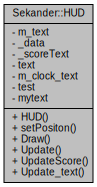
\includegraphics[width=169pt]{classSekander_1_1HUD__coll__graph}
\end{center}
\end{figure}
\subsection*{Public Member Functions}
\begin{DoxyCompactItemize}
\item 
\hyperlink{classSekander_1_1HUD_a36e8acd746cc8528c579f9a443433f49}{H\+UD} (\hyperlink{namespaceSekander_a1d69b002ba2d23020901c28f0def5e16}{Game\+Data\+Ref} data)
\item 
void \hyperlink{classSekander_1_1HUD_adae59bd419e3efb72e52039025cc390d}{set\+Positon} ()
\item 
void \hyperlink{classSekander_1_1HUD_a79da321cb1474c30707d744cf2598fda}{Draw} ()
\item 
void \hyperlink{classSekander_1_1HUD_ad94d4fa9b5d08ee9b8759b581fd7bc00}{Update} ()
\item 
void \hyperlink{classSekander_1_1HUD_a1acd603a773e2ccddb08d7e97a658a01}{Update\+Score} (int score)
\item 
void \hyperlink{classSekander_1_1HUD_a485d26aab99f64815832644f0fba8057}{Update\+\_\+text} (std\+::string)
\end{DoxyCompactItemize}
\subsection*{Private Attributes}
\begin{DoxyCompactItemize}
\item 
sf\+::\+Text \hyperlink{classSekander_1_1HUD_ae30ad06dbe535abf67b75b05c3297b94}{m\+\_\+text}
\item 
\hyperlink{namespaceSekander_a1d69b002ba2d23020901c28f0def5e16}{Game\+Data\+Ref} \hyperlink{classSekander_1_1HUD_a5658d67de64e63fc05a25c09a573e447}{\+\_\+data}
\item 
sf\+::\+Text \hyperlink{classSekander_1_1HUD_a7f6f9251b486bfaf585805959e90bd67}{\+\_\+score\+Text}
\item 
sf\+::\+Text \hyperlink{classSekander_1_1HUD_a840582b62f83a28612a72c703b975ed2}{text}
\item 
sf\+::\+Text \hyperlink{classSekander_1_1HUD_a2687202d5a03a5058b3ac7e388fda66d}{m\+\_\+clock\+\_\+text}
\item 
int \hyperlink{classSekander_1_1HUD_a01751950ac1ddfb126acec810f4e947f}{test} = 1000
\item 
sf\+::\+Text \hyperlink{classSekander_1_1HUD_a73a39d3a2e8b5d648ce9ce738e48b172}{mytext}
\end{DoxyCompactItemize}


\subsection{Constructor \& Destructor Documentation}
\mbox{\Hypertarget{classSekander_1_1HUD_a36e8acd746cc8528c579f9a443433f49}\label{classSekander_1_1HUD_a36e8acd746cc8528c579f9a443433f49}} 
\index{Sekander\+::\+H\+UD@{Sekander\+::\+H\+UD}!H\+UD@{H\+UD}}
\index{H\+UD@{H\+UD}!Sekander\+::\+H\+UD@{Sekander\+::\+H\+UD}}
\subsubsection{\texorpdfstring{H\+U\+D()}{HUD()}}
{\footnotesize\ttfamily Sekander\+::\+H\+U\+D\+::\+H\+UD (\begin{DoxyParamCaption}\item[{\hyperlink{namespaceSekander_a1d69b002ba2d23020901c28f0def5e16}{Game\+Data\+Ref}}]{data }\end{DoxyParamCaption})}



\subsection{Member Function Documentation}
\mbox{\Hypertarget{classSekander_1_1HUD_a79da321cb1474c30707d744cf2598fda}\label{classSekander_1_1HUD_a79da321cb1474c30707d744cf2598fda}} 
\index{Sekander\+::\+H\+UD@{Sekander\+::\+H\+UD}!Draw@{Draw}}
\index{Draw@{Draw}!Sekander\+::\+H\+UD@{Sekander\+::\+H\+UD}}
\subsubsection{\texorpdfstring{Draw()}{Draw()}}
{\footnotesize\ttfamily void Sekander\+::\+H\+U\+D\+::\+Draw (\begin{DoxyParamCaption}{ }\end{DoxyParamCaption})}

\mbox{\Hypertarget{classSekander_1_1HUD_adae59bd419e3efb72e52039025cc390d}\label{classSekander_1_1HUD_adae59bd419e3efb72e52039025cc390d}} 
\index{Sekander\+::\+H\+UD@{Sekander\+::\+H\+UD}!set\+Positon@{set\+Positon}}
\index{set\+Positon@{set\+Positon}!Sekander\+::\+H\+UD@{Sekander\+::\+H\+UD}}
\subsubsection{\texorpdfstring{set\+Positon()}{setPositon()}}
{\footnotesize\ttfamily void Sekander\+::\+H\+U\+D\+::set\+Positon (\begin{DoxyParamCaption}{ }\end{DoxyParamCaption})}

\mbox{\Hypertarget{classSekander_1_1HUD_ad94d4fa9b5d08ee9b8759b581fd7bc00}\label{classSekander_1_1HUD_ad94d4fa9b5d08ee9b8759b581fd7bc00}} 
\index{Sekander\+::\+H\+UD@{Sekander\+::\+H\+UD}!Update@{Update}}
\index{Update@{Update}!Sekander\+::\+H\+UD@{Sekander\+::\+H\+UD}}
\subsubsection{\texorpdfstring{Update()}{Update()}}
{\footnotesize\ttfamily void Sekander\+::\+H\+U\+D\+::\+Update (\begin{DoxyParamCaption}{ }\end{DoxyParamCaption})}

\mbox{\Hypertarget{classSekander_1_1HUD_a485d26aab99f64815832644f0fba8057}\label{classSekander_1_1HUD_a485d26aab99f64815832644f0fba8057}} 
\index{Sekander\+::\+H\+UD@{Sekander\+::\+H\+UD}!Update\+\_\+text@{Update\+\_\+text}}
\index{Update\+\_\+text@{Update\+\_\+text}!Sekander\+::\+H\+UD@{Sekander\+::\+H\+UD}}
\subsubsection{\texorpdfstring{Update\+\_\+text()}{Update\_text()}}
{\footnotesize\ttfamily void Sekander\+::\+H\+U\+D\+::\+Update\+\_\+text (\begin{DoxyParamCaption}\item[{std\+::string}]{s }\end{DoxyParamCaption})}

\mbox{\Hypertarget{classSekander_1_1HUD_a1acd603a773e2ccddb08d7e97a658a01}\label{classSekander_1_1HUD_a1acd603a773e2ccddb08d7e97a658a01}} 
\index{Sekander\+::\+H\+UD@{Sekander\+::\+H\+UD}!Update\+Score@{Update\+Score}}
\index{Update\+Score@{Update\+Score}!Sekander\+::\+H\+UD@{Sekander\+::\+H\+UD}}
\subsubsection{\texorpdfstring{Update\+Score()}{UpdateScore()}}
{\footnotesize\ttfamily void Sekander\+::\+H\+U\+D\+::\+Update\+Score (\begin{DoxyParamCaption}\item[{int}]{score }\end{DoxyParamCaption})}



\subsection{Member Data Documentation}
\mbox{\Hypertarget{classSekander_1_1HUD_a5658d67de64e63fc05a25c09a573e447}\label{classSekander_1_1HUD_a5658d67de64e63fc05a25c09a573e447}} 
\index{Sekander\+::\+H\+UD@{Sekander\+::\+H\+UD}!\+\_\+data@{\+\_\+data}}
\index{\+\_\+data@{\+\_\+data}!Sekander\+::\+H\+UD@{Sekander\+::\+H\+UD}}
\subsubsection{\texorpdfstring{\+\_\+data}{\_data}}
{\footnotesize\ttfamily \hyperlink{namespaceSekander_a1d69b002ba2d23020901c28f0def5e16}{Game\+Data\+Ref} Sekander\+::\+H\+U\+D\+::\+\_\+data\hspace{0.3cm}{\ttfamily [private]}}

\mbox{\Hypertarget{classSekander_1_1HUD_a7f6f9251b486bfaf585805959e90bd67}\label{classSekander_1_1HUD_a7f6f9251b486bfaf585805959e90bd67}} 
\index{Sekander\+::\+H\+UD@{Sekander\+::\+H\+UD}!\+\_\+score\+Text@{\+\_\+score\+Text}}
\index{\+\_\+score\+Text@{\+\_\+score\+Text}!Sekander\+::\+H\+UD@{Sekander\+::\+H\+UD}}
\subsubsection{\texorpdfstring{\+\_\+score\+Text}{\_scoreText}}
{\footnotesize\ttfamily sf\+::\+Text Sekander\+::\+H\+U\+D\+::\+\_\+score\+Text\hspace{0.3cm}{\ttfamily [private]}}

\mbox{\Hypertarget{classSekander_1_1HUD_a2687202d5a03a5058b3ac7e388fda66d}\label{classSekander_1_1HUD_a2687202d5a03a5058b3ac7e388fda66d}} 
\index{Sekander\+::\+H\+UD@{Sekander\+::\+H\+UD}!m\+\_\+clock\+\_\+text@{m\+\_\+clock\+\_\+text}}
\index{m\+\_\+clock\+\_\+text@{m\+\_\+clock\+\_\+text}!Sekander\+::\+H\+UD@{Sekander\+::\+H\+UD}}
\subsubsection{\texorpdfstring{m\+\_\+clock\+\_\+text}{m\_clock\_text}}
{\footnotesize\ttfamily sf\+::\+Text Sekander\+::\+H\+U\+D\+::m\+\_\+clock\+\_\+text\hspace{0.3cm}{\ttfamily [private]}}

\mbox{\Hypertarget{classSekander_1_1HUD_ae30ad06dbe535abf67b75b05c3297b94}\label{classSekander_1_1HUD_ae30ad06dbe535abf67b75b05c3297b94}} 
\index{Sekander\+::\+H\+UD@{Sekander\+::\+H\+UD}!m\+\_\+text@{m\+\_\+text}}
\index{m\+\_\+text@{m\+\_\+text}!Sekander\+::\+H\+UD@{Sekander\+::\+H\+UD}}
\subsubsection{\texorpdfstring{m\+\_\+text}{m\_text}}
{\footnotesize\ttfamily sf\+::\+Text Sekander\+::\+H\+U\+D\+::m\+\_\+text\hspace{0.3cm}{\ttfamily [private]}}

\mbox{\Hypertarget{classSekander_1_1HUD_a73a39d3a2e8b5d648ce9ce738e48b172}\label{classSekander_1_1HUD_a73a39d3a2e8b5d648ce9ce738e48b172}} 
\index{Sekander\+::\+H\+UD@{Sekander\+::\+H\+UD}!mytext@{mytext}}
\index{mytext@{mytext}!Sekander\+::\+H\+UD@{Sekander\+::\+H\+UD}}
\subsubsection{\texorpdfstring{mytext}{mytext}}
{\footnotesize\ttfamily sf\+::\+Text Sekander\+::\+H\+U\+D\+::mytext\hspace{0.3cm}{\ttfamily [private]}}

\mbox{\Hypertarget{classSekander_1_1HUD_a01751950ac1ddfb126acec810f4e947f}\label{classSekander_1_1HUD_a01751950ac1ddfb126acec810f4e947f}} 
\index{Sekander\+::\+H\+UD@{Sekander\+::\+H\+UD}!test@{test}}
\index{test@{test}!Sekander\+::\+H\+UD@{Sekander\+::\+H\+UD}}
\subsubsection{\texorpdfstring{test}{test}}
{\footnotesize\ttfamily int Sekander\+::\+H\+U\+D\+::test = 1000\hspace{0.3cm}{\ttfamily [private]}}

\mbox{\Hypertarget{classSekander_1_1HUD_a840582b62f83a28612a72c703b975ed2}\label{classSekander_1_1HUD_a840582b62f83a28612a72c703b975ed2}} 
\index{Sekander\+::\+H\+UD@{Sekander\+::\+H\+UD}!text@{text}}
\index{text@{text}!Sekander\+::\+H\+UD@{Sekander\+::\+H\+UD}}
\subsubsection{\texorpdfstring{text}{text}}
{\footnotesize\ttfamily sf\+::\+Text Sekander\+::\+H\+U\+D\+::text\hspace{0.3cm}{\ttfamily [private]}}



The documentation for this class was generated from the following files\+:\begin{DoxyCompactItemize}
\item 
/mnt/hdd/\+C0de/\+Engines/\+S\+F\+M\+L/\+S\+F\+M\+L\+\_\+\+Engine/include/\hyperlink{HUD_8hpp}{H\+U\+D.\+hpp}\item 
/mnt/hdd/\+C0de/\+Engines/\+S\+F\+M\+L/\+S\+F\+M\+L\+\_\+\+Engine/src/\hyperlink{HUD_8cpp}{H\+U\+D.\+cpp}\end{DoxyCompactItemize}

\hypertarget{classSekander_1_1InputManager}{}\section{Sekander\+:\+:Input\+Manager Class Reference}
\label{classSekander_1_1InputManager}\index{Sekander\+::\+Input\+Manager@{Sekander\+::\+Input\+Manager}}


{\ttfamily \#include $<$Input\+Manager.\+hpp$>$}



Collaboration diagram for Sekander\+:\+:Input\+Manager\+:
\nopagebreak
\begin{figure}[H]
\begin{center}
\leavevmode
\includegraphics[width=203pt]{classSekander_1_1InputManager__coll__graph}
\end{center}
\end{figure}
\subsection*{Public Member Functions}
\begin{DoxyCompactItemize}
\item 
\hyperlink{classSekander_1_1InputManager_ab171e3428df1026155f91bbb49fe5a4a}{Input\+Manager} ()
\item 
\hyperlink{classSekander_1_1InputManager_ade61718adb0fa9db1a428e3ce6332542}{$\sim$\+Input\+Manager} ()
\item 
bool \hyperlink{classSekander_1_1InputManager_a45b7707b3c38d463a9624624a903a35a}{Is\+Sprite\+Clicked} (sf\+::\+Sprite object, sf\+::\+Mouse\+::\+Button button, sf\+::\+Render\+Window \&window)
\item 
bool \hyperlink{classSekander_1_1InputManager_a66707c739a6e5abc424aba01e6188eef}{Is\+Key\+Pressed} (sf\+::\+Keyboard key)
\item 
sf\+::\+Vector2i \hyperlink{classSekander_1_1InputManager_a6e246fd32b5006e4e5097bbf9dcaea4c}{Get\+Mouse\+Position} (sf\+::\+Render\+Window \&window)
\end{DoxyCompactItemize}
\subsection*{Private Attributes}
\begin{DoxyCompactItemize}
\item 
sf\+::\+Keyboard \hyperlink{classSekander_1_1InputManager_aea65e79014e4b92dbce7fefae50b0022}{\+\_\+key}
\end{DoxyCompactItemize}


\subsection{Constructor \& Destructor Documentation}
\mbox{\Hypertarget{classSekander_1_1InputManager_ab171e3428df1026155f91bbb49fe5a4a}\label{classSekander_1_1InputManager_ab171e3428df1026155f91bbb49fe5a4a}} 
\index{Sekander\+::\+Input\+Manager@{Sekander\+::\+Input\+Manager}!Input\+Manager@{Input\+Manager}}
\index{Input\+Manager@{Input\+Manager}!Sekander\+::\+Input\+Manager@{Sekander\+::\+Input\+Manager}}
\subsubsection{\texorpdfstring{Input\+Manager()}{InputManager()}}
{\footnotesize\ttfamily Sekander\+::\+Input\+Manager\+::\+Input\+Manager (\begin{DoxyParamCaption}{ }\end{DoxyParamCaption})\hspace{0.3cm}{\ttfamily [inline]}}

\mbox{\Hypertarget{classSekander_1_1InputManager_ade61718adb0fa9db1a428e3ce6332542}\label{classSekander_1_1InputManager_ade61718adb0fa9db1a428e3ce6332542}} 
\index{Sekander\+::\+Input\+Manager@{Sekander\+::\+Input\+Manager}!````~Input\+Manager@{$\sim$\+Input\+Manager}}
\index{````~Input\+Manager@{$\sim$\+Input\+Manager}!Sekander\+::\+Input\+Manager@{Sekander\+::\+Input\+Manager}}
\subsubsection{\texorpdfstring{$\sim$\+Input\+Manager()}{~InputManager()}}
{\footnotesize\ttfamily Sekander\+::\+Input\+Manager\+::$\sim$\+Input\+Manager (\begin{DoxyParamCaption}{ }\end{DoxyParamCaption})\hspace{0.3cm}{\ttfamily [inline]}}



\subsection{Member Function Documentation}
\mbox{\Hypertarget{classSekander_1_1InputManager_a6e246fd32b5006e4e5097bbf9dcaea4c}\label{classSekander_1_1InputManager_a6e246fd32b5006e4e5097bbf9dcaea4c}} 
\index{Sekander\+::\+Input\+Manager@{Sekander\+::\+Input\+Manager}!Get\+Mouse\+Position@{Get\+Mouse\+Position}}
\index{Get\+Mouse\+Position@{Get\+Mouse\+Position}!Sekander\+::\+Input\+Manager@{Sekander\+::\+Input\+Manager}}
\subsubsection{\texorpdfstring{Get\+Mouse\+Position()}{GetMousePosition()}}
{\footnotesize\ttfamily sf\+::\+Vector2i Sekander\+::\+Input\+Manager\+::\+Get\+Mouse\+Position (\begin{DoxyParamCaption}\item[{sf\+::\+Render\+Window \&}]{window }\end{DoxyParamCaption})}

\mbox{\Hypertarget{classSekander_1_1InputManager_a66707c739a6e5abc424aba01e6188eef}\label{classSekander_1_1InputManager_a66707c739a6e5abc424aba01e6188eef}} 
\index{Sekander\+::\+Input\+Manager@{Sekander\+::\+Input\+Manager}!Is\+Key\+Pressed@{Is\+Key\+Pressed}}
\index{Is\+Key\+Pressed@{Is\+Key\+Pressed}!Sekander\+::\+Input\+Manager@{Sekander\+::\+Input\+Manager}}
\subsubsection{\texorpdfstring{Is\+Key\+Pressed()}{IsKeyPressed()}}
{\footnotesize\ttfamily bool Sekander\+::\+Input\+Manager\+::\+Is\+Key\+Pressed (\begin{DoxyParamCaption}\item[{sf\+::\+Keyboard}]{key }\end{DoxyParamCaption})}

\mbox{\Hypertarget{classSekander_1_1InputManager_a45b7707b3c38d463a9624624a903a35a}\label{classSekander_1_1InputManager_a45b7707b3c38d463a9624624a903a35a}} 
\index{Sekander\+::\+Input\+Manager@{Sekander\+::\+Input\+Manager}!Is\+Sprite\+Clicked@{Is\+Sprite\+Clicked}}
\index{Is\+Sprite\+Clicked@{Is\+Sprite\+Clicked}!Sekander\+::\+Input\+Manager@{Sekander\+::\+Input\+Manager}}
\subsubsection{\texorpdfstring{Is\+Sprite\+Clicked()}{IsSpriteClicked()}}
{\footnotesize\ttfamily bool Sekander\+::\+Input\+Manager\+::\+Is\+Sprite\+Clicked (\begin{DoxyParamCaption}\item[{sf\+::\+Sprite}]{object,  }\item[{sf\+::\+Mouse\+::\+Button}]{button,  }\item[{sf\+::\+Render\+Window \&}]{window }\end{DoxyParamCaption})}



\subsection{Member Data Documentation}
\mbox{\Hypertarget{classSekander_1_1InputManager_aea65e79014e4b92dbce7fefae50b0022}\label{classSekander_1_1InputManager_aea65e79014e4b92dbce7fefae50b0022}} 
\index{Sekander\+::\+Input\+Manager@{Sekander\+::\+Input\+Manager}!\+\_\+key@{\+\_\+key}}
\index{\+\_\+key@{\+\_\+key}!Sekander\+::\+Input\+Manager@{Sekander\+::\+Input\+Manager}}
\subsubsection{\texorpdfstring{\+\_\+key}{\_key}}
{\footnotesize\ttfamily sf\+::\+Keyboard Sekander\+::\+Input\+Manager\+::\+\_\+key\hspace{0.3cm}{\ttfamily [private]}}



The documentation for this class was generated from the following files\+:\begin{DoxyCompactItemize}
\item 
/mnt/hdd/\+C0de/\+Engines/\+S\+F\+M\+L/\+S\+F\+M\+L\+\_\+\+Engine/include/\hyperlink{InputManager_8hpp}{Input\+Manager.\+hpp}\item 
/mnt/hdd/\+C0de/\+Engines/\+S\+F\+M\+L/\+S\+F\+M\+L\+\_\+\+Engine/src/\hyperlink{InputManager_8cpp}{Input\+Manager.\+cpp}\end{DoxyCompactItemize}

\hypertarget{classSekander_1_1LoadingGameObjects}{}\section{Sekander\+:\+:Loading\+Game\+Objects Class Reference}
\label{classSekander_1_1LoadingGameObjects}\index{Sekander\+::\+Loading\+Game\+Objects@{Sekander\+::\+Loading\+Game\+Objects}}


{\ttfamily \#include $<$Loading\+Game\+Objects.\+hpp$>$}



Collaboration diagram for Sekander\+:\+:Loading\+Game\+Objects\+:
\nopagebreak
\begin{figure}[H]
\begin{center}
\leavevmode
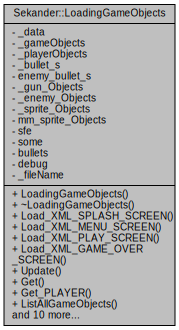
\includegraphics[width=251pt]{classSekander_1_1LoadingGameObjects__coll__graph}
\end{center}
\end{figure}
\subsection*{Public Member Functions}
\begin{DoxyCompactItemize}
\item 
\hyperlink{classSekander_1_1LoadingGameObjects_a05bf4cf5351ede9b00a3c161576c82f1}{Loading\+Game\+Objects} (\hyperlink{namespaceSekander_a1d69b002ba2d23020901c28f0def5e16}{Game\+Data\+Ref} data)
\item 
\hyperlink{classSekander_1_1LoadingGameObjects_ac0a7e1349776ee6cb266f3c3c8cae4ba}{$\sim$\+Loading\+Game\+Objects} ()
\item 
void \hyperlink{classSekander_1_1LoadingGameObjects_a01a3bccc8f858e5cb35d18b58602f3ac}{Load\+\_\+\+X\+M\+L\+\_\+\+S\+P\+L\+A\+S\+H\+\_\+\+S\+C\+R\+E\+EN} (const char $\ast$file\+Name)
\item 
void \hyperlink{classSekander_1_1LoadingGameObjects_ad798b8479b0138f04196e398ab2e2d67}{Load\+\_\+\+X\+M\+L\+\_\+\+M\+E\+N\+U\+\_\+\+S\+C\+R\+E\+EN} (const char $\ast$file\+Name)
\item 
void \hyperlink{classSekander_1_1LoadingGameObjects_a1d4c40b9fe4b0608fd8d40182d37b6d5}{Load\+\_\+\+X\+M\+L\+\_\+\+P\+L\+A\+Y\+\_\+\+S\+C\+R\+E\+EN} (const char $\ast$file\+Name)
\item 
void \hyperlink{classSekander_1_1LoadingGameObjects_a9b1a1dfecbed28a4eef90aa53953cbde}{Load\+\_\+\+X\+M\+L\+\_\+\+G\+A\+M\+E\+\_\+\+O\+V\+E\+R\+\_\+\+S\+C\+R\+E\+EN} (const char $\ast$file\+Name)
\item 
void \hyperlink{classSekander_1_1LoadingGameObjects_a5b665e8cfe17852dad38dd8231004d62}{Update} (float dt)
\item 
\hyperlink{classSekander_1_1GameWorld}{Game\+World} $\ast$ \hyperlink{classSekander_1_1LoadingGameObjects_a489930b1251e3303e1c0d5e7aa90136d}{Get} (const char $\ast$name)
\item 
\hyperlink{classSekander_1_1Main__Player}{Main\+\_\+\+Player} $\ast$ \hyperlink{classSekander_1_1LoadingGameObjects_a6cc5ff99c7f8853a0bb5d002f130ed2d}{Get\+\_\+\+P\+L\+A\+Y\+ER} (const char $\ast$name)
\item 
void \hyperlink{classSekander_1_1LoadingGameObjects_ae13ea38a08bb58ac90279418aac58600}{List\+All\+Game\+Objects} ()
\item 
std\+::unordered\+\_\+map$<$ const char $\ast$, \hyperlink{classSekander_1_1GameWorld}{Game\+World} $\ast$ $>$ \hyperlink{classSekander_1_1LoadingGameObjects_a0b894ea1b1abd089c3e7c5934344ae14}{Get\+\_\+\+Game\+\_\+objects\+\_\+\+Map} ()
\item 
std\+::unordered\+\_\+map$<$ const char $\ast$, \hyperlink{classSekander_1_1Main__Player}{Main\+\_\+\+Player} $\ast$ $>$ \hyperlink{classSekander_1_1LoadingGameObjects_a5561e4d9c2379c0e909e726b2c3a8cfa}{Get\+\_\+\+Player\+\_\+\+Map} ()
\item 
std\+::unordered\+\_\+map$<$ std\+::string, \hyperlink{classSekander_1_1Bullet}{Bullet} $\ast$ $>$ \hyperlink{classSekander_1_1LoadingGameObjects_af3f164ef410cb0c151c55cca1460ae75}{Get\+\_\+\+Bullet\+\_\+\+Map} ()
\item 
std\+::unordered\+\_\+map$<$ std\+::string, \hyperlink{classSekander_1_1Bullet}{Bullet} $\ast$ $>$ \hyperlink{classSekander_1_1LoadingGameObjects_a53cf99dbb68677f73ac858d00173d7f6}{Get\+\_\+\+Enemy\+\_\+\+Bullet\+\_\+\+Map} ()
\item 
std\+::unordered\+\_\+map$<$ const char $\ast$, \hyperlink{classSekander_1_1Gun}{Gun} $\ast$ $>$ \hyperlink{classSekander_1_1LoadingGameObjects_a9917c859d5dd99dd02e48facc068c3ae}{Get\+\_\+\+Gun\+\_\+\+Map} ()
\item 
std\+::unordered\+\_\+map$<$ const char $\ast$, sf\+::\+Sprite $\ast$ $>$ \hyperlink{classSekander_1_1LoadingGameObjects_ac23927738816c3a6bd575483c233d456}{Get\+\_\+\+Sprie\+\_\+\+Map} ()
\item 
std\+::unordered\+\_\+map$<$ std\+::string, sf\+::\+Sprite $\ast$ $>$ \hyperlink{classSekander_1_1LoadingGameObjects_a58857b9a3697137ddf9ad7c161f84fd6}{sd\+Get\+\_\+\+Sprie\+\_\+\+Map} ()
\item 
std\+::unordered\+\_\+map$<$ const char $\ast$, \hyperlink{classSekander_1_1Enemy}{Enemy} $\ast$ $>$ \hyperlink{classSekander_1_1LoadingGameObjects_af1d51f5b67f7476c022f8161323734bd}{Get\+\_\+\+Enemy\+\_\+\+Map} ()
\item 
void \hyperlink{classSekander_1_1LoadingGameObjects_a87c64fc0bc77941f9753e7813e623075}{populate\+\_\+bullets} (int max, std\+::string string\+\_\+key\+\_\+name, std\+::string file\+\_\+name, int source\+\_\+x, int source\+\_\+y, int sprite\+\_\+width, int sprite\+\_\+height, int sprite\+\_\+x\+\_\+frames, int sprite\+\_\+y\+\_\+frames, float x\+\_\+pos, float y\+\_\+pos, float angle)
\item 
void \hyperlink{classSekander_1_1LoadingGameObjects_ae0c8e87b730092dd7129cb9edae07aca}{populate\+\_\+enemy\+\_\+bullets} (int max, std\+::string string\+\_\+key\+\_\+name, std\+::string file\+\_\+name, int source\+\_\+x, int source\+\_\+y, int sprite\+\_\+width, int sprite\+\_\+height, int sprite\+\_\+x\+\_\+frames, int sprite\+\_\+y\+\_\+frames, float x\+\_\+pos, float y\+\_\+pos, float angle)
\end{DoxyCompactItemize}
\subsection*{Private Attributes}
\begin{DoxyCompactItemize}
\item 
\hyperlink{namespaceSekander_a1d69b002ba2d23020901c28f0def5e16}{Game\+Data\+Ref} \hyperlink{classSekander_1_1LoadingGameObjects_aca591b6946d7a71698a91bf97de00f4b}{\+\_\+data}
\item 
std\+::unordered\+\_\+map$<$ const char $\ast$, \hyperlink{classSekander_1_1GameWorld}{Game\+World} $\ast$ $>$ \hyperlink{classSekander_1_1LoadingGameObjects_a7308de0739e761a8b95d300096ee56e1}{\+\_\+game\+Objects}
\item 
std\+::unordered\+\_\+map$<$ const char $\ast$, \hyperlink{classSekander_1_1Main__Player}{Main\+\_\+\+Player} $\ast$ $>$ \hyperlink{classSekander_1_1LoadingGameObjects_accf2f7af898259f2108ef8acc748ac75}{\+\_\+player\+Objects}
\item 
std\+::unordered\+\_\+map$<$ std\+::string,\hyperlink{classSekander_1_1Bullet}{Bullet} $\ast$ $>$ \hyperlink{classSekander_1_1LoadingGameObjects_a6881e7f0dd40a50a243838f59e2b076d}{\+\_\+bullet\+\_\+s}
\item 
std\+::unordered\+\_\+map$<$ std\+::string,\hyperlink{classSekander_1_1Bullet}{Bullet} $\ast$ $>$ \hyperlink{classSekander_1_1LoadingGameObjects_a566b3d1ff614edae05d037a1f44da254}{enemy\+\_\+bullet\+\_\+s}
\item 
std\+::unordered\+\_\+map$<$ const char $\ast$, \hyperlink{classSekander_1_1Gun}{Gun} $\ast$ $>$ \hyperlink{classSekander_1_1LoadingGameObjects_aeedf5c8a6d95e2d67f493c6a342d1550}{\+\_\+gun\+\_\+\+Objects}
\item 
std\+::unordered\+\_\+map$<$ const char $\ast$, \hyperlink{classSekander_1_1Enemy}{Enemy} $\ast$ $>$ \hyperlink{classSekander_1_1LoadingGameObjects_a806a9fe60a9609ccf5b44c9177636074}{\+\_\+enemy\+\_\+\+Objects}
\item 
std\+::unordered\+\_\+map$<$ const char $\ast$, sf\+::\+Sprite $\ast$ $>$ \hyperlink{classSekander_1_1LoadingGameObjects_a27952bf7b7b386de19cad86546823db1}{\+\_\+sprite\+\_\+\+Objects}
\item 
std\+::unordered\+\_\+map$<$ std\+::string, sf\+::\+Sprite $\ast$ $>$ \hyperlink{classSekander_1_1LoadingGameObjects_ae76b503bf88d7696f1a55c38a20f6d01}{mm\+\_\+sprite\+\_\+\+Objects}
\item 
sf\+::\+Sprite $\ast$ \hyperlink{classSekander_1_1LoadingGameObjects_a0c211dbd79d70d20408c7c8eccf9d013}{sfe}
\item 
std\+::vector$<$ std\+::string $>$ \hyperlink{classSekander_1_1LoadingGameObjects_ace89ee79603f4375a65ff4503b18b532}{some}
\item 
std\+::vector$<$ \hyperlink{classSekander_1_1Bullet}{Bullet} $\ast$ $>$ \hyperlink{classSekander_1_1LoadingGameObjects_a6148502878e84a5b56a22aa2916a4e3e}{bullets}
\item 
sf\+::\+Rectangle\+Shape $\ast$ \hyperlink{classSekander_1_1LoadingGameObjects_a14e02163016d771d35045b3ee995a7c0}{debug}
\item 
const char $\ast$ \hyperlink{classSekander_1_1LoadingGameObjects_afeb8ddb9d082cf4187bbe71d0995e4ef}{\+\_\+file\+Name}
\end{DoxyCompactItemize}


\subsection{Constructor \& Destructor Documentation}
\mbox{\Hypertarget{classSekander_1_1LoadingGameObjects_a05bf4cf5351ede9b00a3c161576c82f1}\label{classSekander_1_1LoadingGameObjects_a05bf4cf5351ede9b00a3c161576c82f1}} 
\index{Sekander\+::\+Loading\+Game\+Objects@{Sekander\+::\+Loading\+Game\+Objects}!Loading\+Game\+Objects@{Loading\+Game\+Objects}}
\index{Loading\+Game\+Objects@{Loading\+Game\+Objects}!Sekander\+::\+Loading\+Game\+Objects@{Sekander\+::\+Loading\+Game\+Objects}}
\subsubsection{\texorpdfstring{Loading\+Game\+Objects()}{LoadingGameObjects()}}
{\footnotesize\ttfamily Sekander\+::\+Loading\+Game\+Objects\+::\+Loading\+Game\+Objects (\begin{DoxyParamCaption}\item[{\hyperlink{namespaceSekander_a1d69b002ba2d23020901c28f0def5e16}{Game\+Data\+Ref}}]{data }\end{DoxyParamCaption})}

\mbox{\Hypertarget{classSekander_1_1LoadingGameObjects_ac0a7e1349776ee6cb266f3c3c8cae4ba}\label{classSekander_1_1LoadingGameObjects_ac0a7e1349776ee6cb266f3c3c8cae4ba}} 
\index{Sekander\+::\+Loading\+Game\+Objects@{Sekander\+::\+Loading\+Game\+Objects}!````~Loading\+Game\+Objects@{$\sim$\+Loading\+Game\+Objects}}
\index{````~Loading\+Game\+Objects@{$\sim$\+Loading\+Game\+Objects}!Sekander\+::\+Loading\+Game\+Objects@{Sekander\+::\+Loading\+Game\+Objects}}
\subsubsection{\texorpdfstring{$\sim$\+Loading\+Game\+Objects()}{~LoadingGameObjects()}}
{\footnotesize\ttfamily Sekander\+::\+Loading\+Game\+Objects\+::$\sim$\+Loading\+Game\+Objects (\begin{DoxyParamCaption}{ }\end{DoxyParamCaption})}



\subsection{Member Function Documentation}
\mbox{\Hypertarget{classSekander_1_1LoadingGameObjects_a489930b1251e3303e1c0d5e7aa90136d}\label{classSekander_1_1LoadingGameObjects_a489930b1251e3303e1c0d5e7aa90136d}} 
\index{Sekander\+::\+Loading\+Game\+Objects@{Sekander\+::\+Loading\+Game\+Objects}!Get@{Get}}
\index{Get@{Get}!Sekander\+::\+Loading\+Game\+Objects@{Sekander\+::\+Loading\+Game\+Objects}}
\subsubsection{\texorpdfstring{Get()}{Get()}}
{\footnotesize\ttfamily \hyperlink{classSekander_1_1GameWorld}{Game\+World} $\ast$ Sekander\+::\+Loading\+Game\+Objects\+::\+Get (\begin{DoxyParamCaption}\item[{const char $\ast$}]{name }\end{DoxyParamCaption})}

\mbox{\Hypertarget{classSekander_1_1LoadingGameObjects_af3f164ef410cb0c151c55cca1460ae75}\label{classSekander_1_1LoadingGameObjects_af3f164ef410cb0c151c55cca1460ae75}} 
\index{Sekander\+::\+Loading\+Game\+Objects@{Sekander\+::\+Loading\+Game\+Objects}!Get\+\_\+\+Bullet\+\_\+\+Map@{Get\+\_\+\+Bullet\+\_\+\+Map}}
\index{Get\+\_\+\+Bullet\+\_\+\+Map@{Get\+\_\+\+Bullet\+\_\+\+Map}!Sekander\+::\+Loading\+Game\+Objects@{Sekander\+::\+Loading\+Game\+Objects}}
\subsubsection{\texorpdfstring{Get\+\_\+\+Bullet\+\_\+\+Map()}{Get\_Bullet\_Map()}}
{\footnotesize\ttfamily std\+::unordered\+\_\+map$<$std\+::string, \hyperlink{classSekander_1_1Bullet}{Bullet}$\ast$$>$ Sekander\+::\+Loading\+Game\+Objects\+::\+Get\+\_\+\+Bullet\+\_\+\+Map (\begin{DoxyParamCaption}{ }\end{DoxyParamCaption})\hspace{0.3cm}{\ttfamily [inline]}}

\mbox{\Hypertarget{classSekander_1_1LoadingGameObjects_a53cf99dbb68677f73ac858d00173d7f6}\label{classSekander_1_1LoadingGameObjects_a53cf99dbb68677f73ac858d00173d7f6}} 
\index{Sekander\+::\+Loading\+Game\+Objects@{Sekander\+::\+Loading\+Game\+Objects}!Get\+\_\+\+Enemy\+\_\+\+Bullet\+\_\+\+Map@{Get\+\_\+\+Enemy\+\_\+\+Bullet\+\_\+\+Map}}
\index{Get\+\_\+\+Enemy\+\_\+\+Bullet\+\_\+\+Map@{Get\+\_\+\+Enemy\+\_\+\+Bullet\+\_\+\+Map}!Sekander\+::\+Loading\+Game\+Objects@{Sekander\+::\+Loading\+Game\+Objects}}
\subsubsection{\texorpdfstring{Get\+\_\+\+Enemy\+\_\+\+Bullet\+\_\+\+Map()}{Get\_Enemy\_Bullet\_Map()}}
{\footnotesize\ttfamily std\+::unordered\+\_\+map$<$std\+::string, \hyperlink{classSekander_1_1Bullet}{Bullet}$\ast$$>$ Sekander\+::\+Loading\+Game\+Objects\+::\+Get\+\_\+\+Enemy\+\_\+\+Bullet\+\_\+\+Map (\begin{DoxyParamCaption}{ }\end{DoxyParamCaption})\hspace{0.3cm}{\ttfamily [inline]}}

\mbox{\Hypertarget{classSekander_1_1LoadingGameObjects_af1d51f5b67f7476c022f8161323734bd}\label{classSekander_1_1LoadingGameObjects_af1d51f5b67f7476c022f8161323734bd}} 
\index{Sekander\+::\+Loading\+Game\+Objects@{Sekander\+::\+Loading\+Game\+Objects}!Get\+\_\+\+Enemy\+\_\+\+Map@{Get\+\_\+\+Enemy\+\_\+\+Map}}
\index{Get\+\_\+\+Enemy\+\_\+\+Map@{Get\+\_\+\+Enemy\+\_\+\+Map}!Sekander\+::\+Loading\+Game\+Objects@{Sekander\+::\+Loading\+Game\+Objects}}
\subsubsection{\texorpdfstring{Get\+\_\+\+Enemy\+\_\+\+Map()}{Get\_Enemy\_Map()}}
{\footnotesize\ttfamily std\+::unordered\+\_\+map$<$const char$\ast$, \hyperlink{classSekander_1_1Enemy}{Enemy}$\ast$$>$ Sekander\+::\+Loading\+Game\+Objects\+::\+Get\+\_\+\+Enemy\+\_\+\+Map (\begin{DoxyParamCaption}{ }\end{DoxyParamCaption})\hspace{0.3cm}{\ttfamily [inline]}}

\mbox{\Hypertarget{classSekander_1_1LoadingGameObjects_a0b894ea1b1abd089c3e7c5934344ae14}\label{classSekander_1_1LoadingGameObjects_a0b894ea1b1abd089c3e7c5934344ae14}} 
\index{Sekander\+::\+Loading\+Game\+Objects@{Sekander\+::\+Loading\+Game\+Objects}!Get\+\_\+\+Game\+\_\+objects\+\_\+\+Map@{Get\+\_\+\+Game\+\_\+objects\+\_\+\+Map}}
\index{Get\+\_\+\+Game\+\_\+objects\+\_\+\+Map@{Get\+\_\+\+Game\+\_\+objects\+\_\+\+Map}!Sekander\+::\+Loading\+Game\+Objects@{Sekander\+::\+Loading\+Game\+Objects}}
\subsubsection{\texorpdfstring{Get\+\_\+\+Game\+\_\+objects\+\_\+\+Map()}{Get\_Game\_objects\_Map()}}
{\footnotesize\ttfamily std\+::unordered\+\_\+map$<$const char$\ast$, \hyperlink{classSekander_1_1GameWorld}{Game\+World}$\ast$$>$ Sekander\+::\+Loading\+Game\+Objects\+::\+Get\+\_\+\+Game\+\_\+objects\+\_\+\+Map (\begin{DoxyParamCaption}{ }\end{DoxyParamCaption})\hspace{0.3cm}{\ttfamily [inline]}}

\mbox{\Hypertarget{classSekander_1_1LoadingGameObjects_a9917c859d5dd99dd02e48facc068c3ae}\label{classSekander_1_1LoadingGameObjects_a9917c859d5dd99dd02e48facc068c3ae}} 
\index{Sekander\+::\+Loading\+Game\+Objects@{Sekander\+::\+Loading\+Game\+Objects}!Get\+\_\+\+Gun\+\_\+\+Map@{Get\+\_\+\+Gun\+\_\+\+Map}}
\index{Get\+\_\+\+Gun\+\_\+\+Map@{Get\+\_\+\+Gun\+\_\+\+Map}!Sekander\+::\+Loading\+Game\+Objects@{Sekander\+::\+Loading\+Game\+Objects}}
\subsubsection{\texorpdfstring{Get\+\_\+\+Gun\+\_\+\+Map()}{Get\_Gun\_Map()}}
{\footnotesize\ttfamily std\+::unordered\+\_\+map$<$const char$\ast$, \hyperlink{classSekander_1_1Gun}{Gun}$\ast$$>$ Sekander\+::\+Loading\+Game\+Objects\+::\+Get\+\_\+\+Gun\+\_\+\+Map (\begin{DoxyParamCaption}{ }\end{DoxyParamCaption})\hspace{0.3cm}{\ttfamily [inline]}}

\mbox{\Hypertarget{classSekander_1_1LoadingGameObjects_a6cc5ff99c7f8853a0bb5d002f130ed2d}\label{classSekander_1_1LoadingGameObjects_a6cc5ff99c7f8853a0bb5d002f130ed2d}} 
\index{Sekander\+::\+Loading\+Game\+Objects@{Sekander\+::\+Loading\+Game\+Objects}!Get\+\_\+\+P\+L\+A\+Y\+ER@{Get\+\_\+\+P\+L\+A\+Y\+ER}}
\index{Get\+\_\+\+P\+L\+A\+Y\+ER@{Get\+\_\+\+P\+L\+A\+Y\+ER}!Sekander\+::\+Loading\+Game\+Objects@{Sekander\+::\+Loading\+Game\+Objects}}
\subsubsection{\texorpdfstring{Get\+\_\+\+P\+L\+A\+Y\+E\+R()}{Get\_PLAYER()}}
{\footnotesize\ttfamily \hyperlink{classSekander_1_1Main__Player}{Main\+\_\+\+Player} $\ast$ Sekander\+::\+Loading\+Game\+Objects\+::\+Get\+\_\+\+P\+L\+A\+Y\+ER (\begin{DoxyParamCaption}\item[{const char $\ast$}]{name }\end{DoxyParamCaption})}

\mbox{\Hypertarget{classSekander_1_1LoadingGameObjects_a5561e4d9c2379c0e909e726b2c3a8cfa}\label{classSekander_1_1LoadingGameObjects_a5561e4d9c2379c0e909e726b2c3a8cfa}} 
\index{Sekander\+::\+Loading\+Game\+Objects@{Sekander\+::\+Loading\+Game\+Objects}!Get\+\_\+\+Player\+\_\+\+Map@{Get\+\_\+\+Player\+\_\+\+Map}}
\index{Get\+\_\+\+Player\+\_\+\+Map@{Get\+\_\+\+Player\+\_\+\+Map}!Sekander\+::\+Loading\+Game\+Objects@{Sekander\+::\+Loading\+Game\+Objects}}
\subsubsection{\texorpdfstring{Get\+\_\+\+Player\+\_\+\+Map()}{Get\_Player\_Map()}}
{\footnotesize\ttfamily std\+::unordered\+\_\+map$<$const char$\ast$, \hyperlink{classSekander_1_1Main__Player}{Main\+\_\+\+Player}$\ast$$>$ Sekander\+::\+Loading\+Game\+Objects\+::\+Get\+\_\+\+Player\+\_\+\+Map (\begin{DoxyParamCaption}{ }\end{DoxyParamCaption})\hspace{0.3cm}{\ttfamily [inline]}}

\mbox{\Hypertarget{classSekander_1_1LoadingGameObjects_ac23927738816c3a6bd575483c233d456}\label{classSekander_1_1LoadingGameObjects_ac23927738816c3a6bd575483c233d456}} 
\index{Sekander\+::\+Loading\+Game\+Objects@{Sekander\+::\+Loading\+Game\+Objects}!Get\+\_\+\+Sprie\+\_\+\+Map@{Get\+\_\+\+Sprie\+\_\+\+Map}}
\index{Get\+\_\+\+Sprie\+\_\+\+Map@{Get\+\_\+\+Sprie\+\_\+\+Map}!Sekander\+::\+Loading\+Game\+Objects@{Sekander\+::\+Loading\+Game\+Objects}}
\subsubsection{\texorpdfstring{Get\+\_\+\+Sprie\+\_\+\+Map()}{Get\_Sprie\_Map()}}
{\footnotesize\ttfamily std\+::unordered\+\_\+map$<$const char$\ast$, sf\+::\+Sprite$\ast$$>$ Sekander\+::\+Loading\+Game\+Objects\+::\+Get\+\_\+\+Sprie\+\_\+\+Map (\begin{DoxyParamCaption}{ }\end{DoxyParamCaption})\hspace{0.3cm}{\ttfamily [inline]}}

\mbox{\Hypertarget{classSekander_1_1LoadingGameObjects_ae13ea38a08bb58ac90279418aac58600}\label{classSekander_1_1LoadingGameObjects_ae13ea38a08bb58ac90279418aac58600}} 
\index{Sekander\+::\+Loading\+Game\+Objects@{Sekander\+::\+Loading\+Game\+Objects}!List\+All\+Game\+Objects@{List\+All\+Game\+Objects}}
\index{List\+All\+Game\+Objects@{List\+All\+Game\+Objects}!Sekander\+::\+Loading\+Game\+Objects@{Sekander\+::\+Loading\+Game\+Objects}}
\subsubsection{\texorpdfstring{List\+All\+Game\+Objects()}{ListAllGameObjects()}}
{\footnotesize\ttfamily void Sekander\+::\+Loading\+Game\+Objects\+::\+List\+All\+Game\+Objects (\begin{DoxyParamCaption}{ }\end{DoxyParamCaption})}

\mbox{\Hypertarget{classSekander_1_1LoadingGameObjects_a9b1a1dfecbed28a4eef90aa53953cbde}\label{classSekander_1_1LoadingGameObjects_a9b1a1dfecbed28a4eef90aa53953cbde}} 
\index{Sekander\+::\+Loading\+Game\+Objects@{Sekander\+::\+Loading\+Game\+Objects}!Load\+\_\+\+X\+M\+L\+\_\+\+G\+A\+M\+E\+\_\+\+O\+V\+E\+R\+\_\+\+S\+C\+R\+E\+EN@{Load\+\_\+\+X\+M\+L\+\_\+\+G\+A\+M\+E\+\_\+\+O\+V\+E\+R\+\_\+\+S\+C\+R\+E\+EN}}
\index{Load\+\_\+\+X\+M\+L\+\_\+\+G\+A\+M\+E\+\_\+\+O\+V\+E\+R\+\_\+\+S\+C\+R\+E\+EN@{Load\+\_\+\+X\+M\+L\+\_\+\+G\+A\+M\+E\+\_\+\+O\+V\+E\+R\+\_\+\+S\+C\+R\+E\+EN}!Sekander\+::\+Loading\+Game\+Objects@{Sekander\+::\+Loading\+Game\+Objects}}
\subsubsection{\texorpdfstring{Load\+\_\+\+X\+M\+L\+\_\+\+G\+A\+M\+E\+\_\+\+O\+V\+E\+R\+\_\+\+S\+C\+R\+E\+E\+N()}{Load\_XML\_GAME\_OVER\_SCREEN()}}
{\footnotesize\ttfamily void Sekander\+::\+Loading\+Game\+Objects\+::\+Load\+\_\+\+X\+M\+L\+\_\+\+G\+A\+M\+E\+\_\+\+O\+V\+E\+R\+\_\+\+S\+C\+R\+E\+EN (\begin{DoxyParamCaption}\item[{const char $\ast$}]{file\+Name }\end{DoxyParamCaption})}

\mbox{\Hypertarget{classSekander_1_1LoadingGameObjects_ad798b8479b0138f04196e398ab2e2d67}\label{classSekander_1_1LoadingGameObjects_ad798b8479b0138f04196e398ab2e2d67}} 
\index{Sekander\+::\+Loading\+Game\+Objects@{Sekander\+::\+Loading\+Game\+Objects}!Load\+\_\+\+X\+M\+L\+\_\+\+M\+E\+N\+U\+\_\+\+S\+C\+R\+E\+EN@{Load\+\_\+\+X\+M\+L\+\_\+\+M\+E\+N\+U\+\_\+\+S\+C\+R\+E\+EN}}
\index{Load\+\_\+\+X\+M\+L\+\_\+\+M\+E\+N\+U\+\_\+\+S\+C\+R\+E\+EN@{Load\+\_\+\+X\+M\+L\+\_\+\+M\+E\+N\+U\+\_\+\+S\+C\+R\+E\+EN}!Sekander\+::\+Loading\+Game\+Objects@{Sekander\+::\+Loading\+Game\+Objects}}
\subsubsection{\texorpdfstring{Load\+\_\+\+X\+M\+L\+\_\+\+M\+E\+N\+U\+\_\+\+S\+C\+R\+E\+E\+N()}{Load\_XML\_MENU\_SCREEN()}}
{\footnotesize\ttfamily void Sekander\+::\+Loading\+Game\+Objects\+::\+Load\+\_\+\+X\+M\+L\+\_\+\+M\+E\+N\+U\+\_\+\+S\+C\+R\+E\+EN (\begin{DoxyParamCaption}\item[{const char $\ast$}]{file\+Name }\end{DoxyParamCaption})}

\mbox{\Hypertarget{classSekander_1_1LoadingGameObjects_a1d4c40b9fe4b0608fd8d40182d37b6d5}\label{classSekander_1_1LoadingGameObjects_a1d4c40b9fe4b0608fd8d40182d37b6d5}} 
\index{Sekander\+::\+Loading\+Game\+Objects@{Sekander\+::\+Loading\+Game\+Objects}!Load\+\_\+\+X\+M\+L\+\_\+\+P\+L\+A\+Y\+\_\+\+S\+C\+R\+E\+EN@{Load\+\_\+\+X\+M\+L\+\_\+\+P\+L\+A\+Y\+\_\+\+S\+C\+R\+E\+EN}}
\index{Load\+\_\+\+X\+M\+L\+\_\+\+P\+L\+A\+Y\+\_\+\+S\+C\+R\+E\+EN@{Load\+\_\+\+X\+M\+L\+\_\+\+P\+L\+A\+Y\+\_\+\+S\+C\+R\+E\+EN}!Sekander\+::\+Loading\+Game\+Objects@{Sekander\+::\+Loading\+Game\+Objects}}
\subsubsection{\texorpdfstring{Load\+\_\+\+X\+M\+L\+\_\+\+P\+L\+A\+Y\+\_\+\+S\+C\+R\+E\+E\+N()}{Load\_XML\_PLAY\_SCREEN()}}
{\footnotesize\ttfamily void Sekander\+::\+Loading\+Game\+Objects\+::\+Load\+\_\+\+X\+M\+L\+\_\+\+P\+L\+A\+Y\+\_\+\+S\+C\+R\+E\+EN (\begin{DoxyParamCaption}\item[{const char $\ast$}]{file\+Name }\end{DoxyParamCaption})}

\mbox{\Hypertarget{classSekander_1_1LoadingGameObjects_a01a3bccc8f858e5cb35d18b58602f3ac}\label{classSekander_1_1LoadingGameObjects_a01a3bccc8f858e5cb35d18b58602f3ac}} 
\index{Sekander\+::\+Loading\+Game\+Objects@{Sekander\+::\+Loading\+Game\+Objects}!Load\+\_\+\+X\+M\+L\+\_\+\+S\+P\+L\+A\+S\+H\+\_\+\+S\+C\+R\+E\+EN@{Load\+\_\+\+X\+M\+L\+\_\+\+S\+P\+L\+A\+S\+H\+\_\+\+S\+C\+R\+E\+EN}}
\index{Load\+\_\+\+X\+M\+L\+\_\+\+S\+P\+L\+A\+S\+H\+\_\+\+S\+C\+R\+E\+EN@{Load\+\_\+\+X\+M\+L\+\_\+\+S\+P\+L\+A\+S\+H\+\_\+\+S\+C\+R\+E\+EN}!Sekander\+::\+Loading\+Game\+Objects@{Sekander\+::\+Loading\+Game\+Objects}}
\subsubsection{\texorpdfstring{Load\+\_\+\+X\+M\+L\+\_\+\+S\+P\+L\+A\+S\+H\+\_\+\+S\+C\+R\+E\+E\+N()}{Load\_XML\_SPLASH\_SCREEN()}}
{\footnotesize\ttfamily void Sekander\+::\+Loading\+Game\+Objects\+::\+Load\+\_\+\+X\+M\+L\+\_\+\+S\+P\+L\+A\+S\+H\+\_\+\+S\+C\+R\+E\+EN (\begin{DoxyParamCaption}\item[{const char $\ast$}]{file\+Name }\end{DoxyParamCaption})}

\mbox{\Hypertarget{classSekander_1_1LoadingGameObjects_a87c64fc0bc77941f9753e7813e623075}\label{classSekander_1_1LoadingGameObjects_a87c64fc0bc77941f9753e7813e623075}} 
\index{Sekander\+::\+Loading\+Game\+Objects@{Sekander\+::\+Loading\+Game\+Objects}!populate\+\_\+bullets@{populate\+\_\+bullets}}
\index{populate\+\_\+bullets@{populate\+\_\+bullets}!Sekander\+::\+Loading\+Game\+Objects@{Sekander\+::\+Loading\+Game\+Objects}}
\subsubsection{\texorpdfstring{populate\+\_\+bullets()}{populate\_bullets()}}
{\footnotesize\ttfamily void Sekander\+::\+Loading\+Game\+Objects\+::populate\+\_\+bullets (\begin{DoxyParamCaption}\item[{int}]{max,  }\item[{std\+::string}]{string\+\_\+key\+\_\+name,  }\item[{std\+::string}]{file\+\_\+name,  }\item[{int}]{source\+\_\+x,  }\item[{int}]{source\+\_\+y,  }\item[{int}]{sprite\+\_\+width,  }\item[{int}]{sprite\+\_\+height,  }\item[{int}]{sprite\+\_\+x\+\_\+frames,  }\item[{int}]{sprite\+\_\+y\+\_\+frames,  }\item[{float}]{x\+\_\+pos,  }\item[{float}]{y\+\_\+pos,  }\item[{float}]{angle }\end{DoxyParamCaption})\hspace{0.3cm}{\ttfamily [inline]}}

\mbox{\Hypertarget{classSekander_1_1LoadingGameObjects_ae0c8e87b730092dd7129cb9edae07aca}\label{classSekander_1_1LoadingGameObjects_ae0c8e87b730092dd7129cb9edae07aca}} 
\index{Sekander\+::\+Loading\+Game\+Objects@{Sekander\+::\+Loading\+Game\+Objects}!populate\+\_\+enemy\+\_\+bullets@{populate\+\_\+enemy\+\_\+bullets}}
\index{populate\+\_\+enemy\+\_\+bullets@{populate\+\_\+enemy\+\_\+bullets}!Sekander\+::\+Loading\+Game\+Objects@{Sekander\+::\+Loading\+Game\+Objects}}
\subsubsection{\texorpdfstring{populate\+\_\+enemy\+\_\+bullets()}{populate\_enemy\_bullets()}}
{\footnotesize\ttfamily void Sekander\+::\+Loading\+Game\+Objects\+::populate\+\_\+enemy\+\_\+bullets (\begin{DoxyParamCaption}\item[{int}]{max,  }\item[{std\+::string}]{string\+\_\+key\+\_\+name,  }\item[{std\+::string}]{file\+\_\+name,  }\item[{int}]{source\+\_\+x,  }\item[{int}]{source\+\_\+y,  }\item[{int}]{sprite\+\_\+width,  }\item[{int}]{sprite\+\_\+height,  }\item[{int}]{sprite\+\_\+x\+\_\+frames,  }\item[{int}]{sprite\+\_\+y\+\_\+frames,  }\item[{float}]{x\+\_\+pos,  }\item[{float}]{y\+\_\+pos,  }\item[{float}]{angle }\end{DoxyParamCaption})\hspace{0.3cm}{\ttfamily [inline]}}

\mbox{\Hypertarget{classSekander_1_1LoadingGameObjects_a58857b9a3697137ddf9ad7c161f84fd6}\label{classSekander_1_1LoadingGameObjects_a58857b9a3697137ddf9ad7c161f84fd6}} 
\index{Sekander\+::\+Loading\+Game\+Objects@{Sekander\+::\+Loading\+Game\+Objects}!sd\+Get\+\_\+\+Sprie\+\_\+\+Map@{sd\+Get\+\_\+\+Sprie\+\_\+\+Map}}
\index{sd\+Get\+\_\+\+Sprie\+\_\+\+Map@{sd\+Get\+\_\+\+Sprie\+\_\+\+Map}!Sekander\+::\+Loading\+Game\+Objects@{Sekander\+::\+Loading\+Game\+Objects}}
\subsubsection{\texorpdfstring{sd\+Get\+\_\+\+Sprie\+\_\+\+Map()}{sdGet\_Sprie\_Map()}}
{\footnotesize\ttfamily std\+::unordered\+\_\+map$<$std\+::string, sf\+::\+Sprite$\ast$$>$ Sekander\+::\+Loading\+Game\+Objects\+::sd\+Get\+\_\+\+Sprie\+\_\+\+Map (\begin{DoxyParamCaption}{ }\end{DoxyParamCaption})\hspace{0.3cm}{\ttfamily [inline]}}

\mbox{\Hypertarget{classSekander_1_1LoadingGameObjects_a5b665e8cfe17852dad38dd8231004d62}\label{classSekander_1_1LoadingGameObjects_a5b665e8cfe17852dad38dd8231004d62}} 
\index{Sekander\+::\+Loading\+Game\+Objects@{Sekander\+::\+Loading\+Game\+Objects}!Update@{Update}}
\index{Update@{Update}!Sekander\+::\+Loading\+Game\+Objects@{Sekander\+::\+Loading\+Game\+Objects}}
\subsubsection{\texorpdfstring{Update()}{Update()}}
{\footnotesize\ttfamily void Sekander\+::\+Loading\+Game\+Objects\+::\+Update (\begin{DoxyParamCaption}\item[{float}]{dt }\end{DoxyParamCaption})}



\subsection{Member Data Documentation}
\mbox{\Hypertarget{classSekander_1_1LoadingGameObjects_a6881e7f0dd40a50a243838f59e2b076d}\label{classSekander_1_1LoadingGameObjects_a6881e7f0dd40a50a243838f59e2b076d}} 
\index{Sekander\+::\+Loading\+Game\+Objects@{Sekander\+::\+Loading\+Game\+Objects}!\+\_\+bullet\+\_\+s@{\+\_\+bullet\+\_\+s}}
\index{\+\_\+bullet\+\_\+s@{\+\_\+bullet\+\_\+s}!Sekander\+::\+Loading\+Game\+Objects@{Sekander\+::\+Loading\+Game\+Objects}}
\subsubsection{\texorpdfstring{\+\_\+bullet\+\_\+s}{\_bullet\_s}}
{\footnotesize\ttfamily std\+::unordered\+\_\+map$<$std\+::string ,\hyperlink{classSekander_1_1Bullet}{Bullet}$\ast$$>$ Sekander\+::\+Loading\+Game\+Objects\+::\+\_\+bullet\+\_\+s\hspace{0.3cm}{\ttfamily [private]}}

\mbox{\Hypertarget{classSekander_1_1LoadingGameObjects_aca591b6946d7a71698a91bf97de00f4b}\label{classSekander_1_1LoadingGameObjects_aca591b6946d7a71698a91bf97de00f4b}} 
\index{Sekander\+::\+Loading\+Game\+Objects@{Sekander\+::\+Loading\+Game\+Objects}!\+\_\+data@{\+\_\+data}}
\index{\+\_\+data@{\+\_\+data}!Sekander\+::\+Loading\+Game\+Objects@{Sekander\+::\+Loading\+Game\+Objects}}
\subsubsection{\texorpdfstring{\+\_\+data}{\_data}}
{\footnotesize\ttfamily \hyperlink{namespaceSekander_a1d69b002ba2d23020901c28f0def5e16}{Game\+Data\+Ref} Sekander\+::\+Loading\+Game\+Objects\+::\+\_\+data\hspace{0.3cm}{\ttfamily [private]}}

\mbox{\Hypertarget{classSekander_1_1LoadingGameObjects_a806a9fe60a9609ccf5b44c9177636074}\label{classSekander_1_1LoadingGameObjects_a806a9fe60a9609ccf5b44c9177636074}} 
\index{Sekander\+::\+Loading\+Game\+Objects@{Sekander\+::\+Loading\+Game\+Objects}!\+\_\+enemy\+\_\+\+Objects@{\+\_\+enemy\+\_\+\+Objects}}
\index{\+\_\+enemy\+\_\+\+Objects@{\+\_\+enemy\+\_\+\+Objects}!Sekander\+::\+Loading\+Game\+Objects@{Sekander\+::\+Loading\+Game\+Objects}}
\subsubsection{\texorpdfstring{\+\_\+enemy\+\_\+\+Objects}{\_enemy\_Objects}}
{\footnotesize\ttfamily std\+::unordered\+\_\+map$<$const char$\ast$, \hyperlink{classSekander_1_1Enemy}{Enemy}$\ast$$>$ Sekander\+::\+Loading\+Game\+Objects\+::\+\_\+enemy\+\_\+\+Objects\hspace{0.3cm}{\ttfamily [private]}}

\mbox{\Hypertarget{classSekander_1_1LoadingGameObjects_afeb8ddb9d082cf4187bbe71d0995e4ef}\label{classSekander_1_1LoadingGameObjects_afeb8ddb9d082cf4187bbe71d0995e4ef}} 
\index{Sekander\+::\+Loading\+Game\+Objects@{Sekander\+::\+Loading\+Game\+Objects}!\+\_\+file\+Name@{\+\_\+file\+Name}}
\index{\+\_\+file\+Name@{\+\_\+file\+Name}!Sekander\+::\+Loading\+Game\+Objects@{Sekander\+::\+Loading\+Game\+Objects}}
\subsubsection{\texorpdfstring{\+\_\+file\+Name}{\_fileName}}
{\footnotesize\ttfamily const char$\ast$ Sekander\+::\+Loading\+Game\+Objects\+::\+\_\+file\+Name\hspace{0.3cm}{\ttfamily [private]}}

\mbox{\Hypertarget{classSekander_1_1LoadingGameObjects_a7308de0739e761a8b95d300096ee56e1}\label{classSekander_1_1LoadingGameObjects_a7308de0739e761a8b95d300096ee56e1}} 
\index{Sekander\+::\+Loading\+Game\+Objects@{Sekander\+::\+Loading\+Game\+Objects}!\+\_\+game\+Objects@{\+\_\+game\+Objects}}
\index{\+\_\+game\+Objects@{\+\_\+game\+Objects}!Sekander\+::\+Loading\+Game\+Objects@{Sekander\+::\+Loading\+Game\+Objects}}
\subsubsection{\texorpdfstring{\+\_\+game\+Objects}{\_gameObjects}}
{\footnotesize\ttfamily std\+::unordered\+\_\+map$<$const char$\ast$, \hyperlink{classSekander_1_1GameWorld}{Game\+World}$\ast$$>$ Sekander\+::\+Loading\+Game\+Objects\+::\+\_\+game\+Objects\hspace{0.3cm}{\ttfamily [private]}}

\mbox{\Hypertarget{classSekander_1_1LoadingGameObjects_aeedf5c8a6d95e2d67f493c6a342d1550}\label{classSekander_1_1LoadingGameObjects_aeedf5c8a6d95e2d67f493c6a342d1550}} 
\index{Sekander\+::\+Loading\+Game\+Objects@{Sekander\+::\+Loading\+Game\+Objects}!\+\_\+gun\+\_\+\+Objects@{\+\_\+gun\+\_\+\+Objects}}
\index{\+\_\+gun\+\_\+\+Objects@{\+\_\+gun\+\_\+\+Objects}!Sekander\+::\+Loading\+Game\+Objects@{Sekander\+::\+Loading\+Game\+Objects}}
\subsubsection{\texorpdfstring{\+\_\+gun\+\_\+\+Objects}{\_gun\_Objects}}
{\footnotesize\ttfamily std\+::unordered\+\_\+map$<$const char$\ast$, \hyperlink{classSekander_1_1Gun}{Gun}$\ast$$>$ Sekander\+::\+Loading\+Game\+Objects\+::\+\_\+gun\+\_\+\+Objects\hspace{0.3cm}{\ttfamily [private]}}

\mbox{\Hypertarget{classSekander_1_1LoadingGameObjects_accf2f7af898259f2108ef8acc748ac75}\label{classSekander_1_1LoadingGameObjects_accf2f7af898259f2108ef8acc748ac75}} 
\index{Sekander\+::\+Loading\+Game\+Objects@{Sekander\+::\+Loading\+Game\+Objects}!\+\_\+player\+Objects@{\+\_\+player\+Objects}}
\index{\+\_\+player\+Objects@{\+\_\+player\+Objects}!Sekander\+::\+Loading\+Game\+Objects@{Sekander\+::\+Loading\+Game\+Objects}}
\subsubsection{\texorpdfstring{\+\_\+player\+Objects}{\_playerObjects}}
{\footnotesize\ttfamily std\+::unordered\+\_\+map$<$const char$\ast$, \hyperlink{classSekander_1_1Main__Player}{Main\+\_\+\+Player}$\ast$$>$ Sekander\+::\+Loading\+Game\+Objects\+::\+\_\+player\+Objects\hspace{0.3cm}{\ttfamily [private]}}

\mbox{\Hypertarget{classSekander_1_1LoadingGameObjects_a27952bf7b7b386de19cad86546823db1}\label{classSekander_1_1LoadingGameObjects_a27952bf7b7b386de19cad86546823db1}} 
\index{Sekander\+::\+Loading\+Game\+Objects@{Sekander\+::\+Loading\+Game\+Objects}!\+\_\+sprite\+\_\+\+Objects@{\+\_\+sprite\+\_\+\+Objects}}
\index{\+\_\+sprite\+\_\+\+Objects@{\+\_\+sprite\+\_\+\+Objects}!Sekander\+::\+Loading\+Game\+Objects@{Sekander\+::\+Loading\+Game\+Objects}}
\subsubsection{\texorpdfstring{\+\_\+sprite\+\_\+\+Objects}{\_sprite\_Objects}}
{\footnotesize\ttfamily std\+::unordered\+\_\+map$<$const char$\ast$, sf\+::\+Sprite$\ast$$>$ Sekander\+::\+Loading\+Game\+Objects\+::\+\_\+sprite\+\_\+\+Objects\hspace{0.3cm}{\ttfamily [private]}}

\mbox{\Hypertarget{classSekander_1_1LoadingGameObjects_a6148502878e84a5b56a22aa2916a4e3e}\label{classSekander_1_1LoadingGameObjects_a6148502878e84a5b56a22aa2916a4e3e}} 
\index{Sekander\+::\+Loading\+Game\+Objects@{Sekander\+::\+Loading\+Game\+Objects}!bullets@{bullets}}
\index{bullets@{bullets}!Sekander\+::\+Loading\+Game\+Objects@{Sekander\+::\+Loading\+Game\+Objects}}
\subsubsection{\texorpdfstring{bullets}{bullets}}
{\footnotesize\ttfamily std\+::vector$<$\hyperlink{classSekander_1_1Bullet}{Bullet}$\ast$$>$ Sekander\+::\+Loading\+Game\+Objects\+::bullets\hspace{0.3cm}{\ttfamily [private]}}

\mbox{\Hypertarget{classSekander_1_1LoadingGameObjects_a14e02163016d771d35045b3ee995a7c0}\label{classSekander_1_1LoadingGameObjects_a14e02163016d771d35045b3ee995a7c0}} 
\index{Sekander\+::\+Loading\+Game\+Objects@{Sekander\+::\+Loading\+Game\+Objects}!debug@{debug}}
\index{debug@{debug}!Sekander\+::\+Loading\+Game\+Objects@{Sekander\+::\+Loading\+Game\+Objects}}
\subsubsection{\texorpdfstring{debug}{debug}}
{\footnotesize\ttfamily sf\+::\+Rectangle\+Shape$\ast$ Sekander\+::\+Loading\+Game\+Objects\+::debug\hspace{0.3cm}{\ttfamily [private]}}

\mbox{\Hypertarget{classSekander_1_1LoadingGameObjects_a566b3d1ff614edae05d037a1f44da254}\label{classSekander_1_1LoadingGameObjects_a566b3d1ff614edae05d037a1f44da254}} 
\index{Sekander\+::\+Loading\+Game\+Objects@{Sekander\+::\+Loading\+Game\+Objects}!enemy\+\_\+bullet\+\_\+s@{enemy\+\_\+bullet\+\_\+s}}
\index{enemy\+\_\+bullet\+\_\+s@{enemy\+\_\+bullet\+\_\+s}!Sekander\+::\+Loading\+Game\+Objects@{Sekander\+::\+Loading\+Game\+Objects}}
\subsubsection{\texorpdfstring{enemy\+\_\+bullet\+\_\+s}{enemy\_bullet\_s}}
{\footnotesize\ttfamily std\+::unordered\+\_\+map$<$std\+::string ,\hyperlink{classSekander_1_1Bullet}{Bullet}$\ast$$>$ Sekander\+::\+Loading\+Game\+Objects\+::enemy\+\_\+bullet\+\_\+s\hspace{0.3cm}{\ttfamily [private]}}

\mbox{\Hypertarget{classSekander_1_1LoadingGameObjects_ae76b503bf88d7696f1a55c38a20f6d01}\label{classSekander_1_1LoadingGameObjects_ae76b503bf88d7696f1a55c38a20f6d01}} 
\index{Sekander\+::\+Loading\+Game\+Objects@{Sekander\+::\+Loading\+Game\+Objects}!mm\+\_\+sprite\+\_\+\+Objects@{mm\+\_\+sprite\+\_\+\+Objects}}
\index{mm\+\_\+sprite\+\_\+\+Objects@{mm\+\_\+sprite\+\_\+\+Objects}!Sekander\+::\+Loading\+Game\+Objects@{Sekander\+::\+Loading\+Game\+Objects}}
\subsubsection{\texorpdfstring{mm\+\_\+sprite\+\_\+\+Objects}{mm\_sprite\_Objects}}
{\footnotesize\ttfamily std\+::unordered\+\_\+map$<$std\+::string , sf\+::\+Sprite$\ast$$>$ Sekander\+::\+Loading\+Game\+Objects\+::mm\+\_\+sprite\+\_\+\+Objects\hspace{0.3cm}{\ttfamily [private]}}

\mbox{\Hypertarget{classSekander_1_1LoadingGameObjects_a0c211dbd79d70d20408c7c8eccf9d013}\label{classSekander_1_1LoadingGameObjects_a0c211dbd79d70d20408c7c8eccf9d013}} 
\index{Sekander\+::\+Loading\+Game\+Objects@{Sekander\+::\+Loading\+Game\+Objects}!sfe@{sfe}}
\index{sfe@{sfe}!Sekander\+::\+Loading\+Game\+Objects@{Sekander\+::\+Loading\+Game\+Objects}}
\subsubsection{\texorpdfstring{sfe}{sfe}}
{\footnotesize\ttfamily sf\+::\+Sprite$\ast$ Sekander\+::\+Loading\+Game\+Objects\+::sfe\hspace{0.3cm}{\ttfamily [private]}}

\mbox{\Hypertarget{classSekander_1_1LoadingGameObjects_ace89ee79603f4375a65ff4503b18b532}\label{classSekander_1_1LoadingGameObjects_ace89ee79603f4375a65ff4503b18b532}} 
\index{Sekander\+::\+Loading\+Game\+Objects@{Sekander\+::\+Loading\+Game\+Objects}!some@{some}}
\index{some@{some}!Sekander\+::\+Loading\+Game\+Objects@{Sekander\+::\+Loading\+Game\+Objects}}
\subsubsection{\texorpdfstring{some}{some}}
{\footnotesize\ttfamily std\+::vector$<$std\+::string$>$ Sekander\+::\+Loading\+Game\+Objects\+::some\hspace{0.3cm}{\ttfamily [private]}}



The documentation for this class was generated from the following files\+:\begin{DoxyCompactItemize}
\item 
/mnt/hdd/\+C0de/\+Engines/\+S\+F\+M\+L/\+S\+F\+M\+L\+\_\+\+Engine/include/\hyperlink{LoadingGameObjects_8hpp}{Loading\+Game\+Objects.\+hpp}\item 
/mnt/hdd/\+C0de/\+Engines/\+S\+F\+M\+L/\+S\+F\+M\+L\+\_\+\+Engine/src/\hyperlink{LoadingGameObjects_8cpp}{Loading\+Game\+Objects.\+cpp}\end{DoxyCompactItemize}

\hypertarget{classSekander_1_1Main__Player}{}\section{Sekander\+:\+:Main\+\_\+\+Player Class Reference}
\label{classSekander_1_1Main__Player}\index{Sekander\+::\+Main\+\_\+\+Player@{Sekander\+::\+Main\+\_\+\+Player}}


{\ttfamily \#include $<$Main\+\_\+\+Player.\+hpp$>$}



Inheritance diagram for Sekander\+:\+:Main\+\_\+\+Player\+:
\nopagebreak
\begin{figure}[H]
\begin{center}
\leavevmode
\includegraphics[height=550pt]{classSekander_1_1Main__Player__inherit__graph}
\end{center}
\end{figure}


Collaboration diagram for Sekander\+:\+:Main\+\_\+\+Player\+:
\nopagebreak
\begin{figure}[H]
\begin{center}
\leavevmode
\includegraphics[height=550pt]{classSekander_1_1Main__Player__coll__graph}
\end{center}
\end{figure}
\subsection*{Public Member Functions}
\begin{DoxyCompactItemize}
\item 
\hyperlink{classSekander_1_1Main__Player_a3db6385e3bff1d503b9305dd51952371}{Main\+\_\+\+Player} ()
\item 
\hyperlink{classSekander_1_1Main__Player_ad4c368b23e2e27a965a71dd5b5a9b8ba}{Main\+\_\+\+Player} (\hyperlink{namespaceSekander_a1d69b002ba2d23020901c28f0def5e16}{Game\+Data\+Ref} data, std\+::string key, std\+::string file\+\_\+name, int source\+\_\+x, int source\+\_\+y, int sprite\+\_\+\+W\+I\+D\+TH, int sprite\+\_\+\+H\+E\+I\+G\+HT, bool dynamic, int sprite\+\_\+\+X\+\_\+\+F\+R\+A\+M\+ES, int sprite\+\_\+\+Y\+\_\+\+F\+R\+A\+M\+ES, float sprite\+\_\+\+X\+\_\+\+P\+OS, float sprite\+\_\+\+Y\+\_\+\+P\+OS, float sprite\+\_\+\+A\+N\+G\+LE)
\item 
void \hyperlink{classSekander_1_1Main__Player_a5d37beaabf93f7c5b01578334da246a2}{Jump} (bool)
\item 
void \hyperlink{classSekander_1_1Main__Player_af62bb952d58130e6c79bf033c183df20}{Double\+Jump} (bool)
\item 
void \hyperlink{classSekander_1_1Main__Player_aaa5aa69d0e4947e24d3ea326f7142bc5}{Mover\+Up} ()
\item 
void \hyperlink{classSekander_1_1Main__Player_a72cd2d23a9d43627df23bf791d5fe08c}{Mover\+Down} ()
\item 
void \hyperlink{classSekander_1_1Main__Player_a5207bda5738aefb2d905170545f6e373}{Mover\+Rigtht} (float speed)
\item 
void \hyperlink{classSekander_1_1Main__Player_a2745801e5bd672d995a5fda6046535e4}{Dash} ()
\item 
void \hyperlink{classSekander_1_1Main__Player_a4ec697d86cc21197100f1ad5e9428aab}{Shooting} (\hyperlink{classSekander_1_1Gun}{Gun} \&, std\+::unordered\+\_\+map$<$ std\+::string, \hyperlink{classSekander_1_1Bullet}{Bullet} $\ast$$>$)
\item 
void \hyperlink{classSekander_1_1Main__Player_a870cb1809cf55fa050558d40c2d6f487}{N\+U\+\_\+\+Shooting} (\hyperlink{classSekander_1_1Gun}{Gun} \&)
\item 
void \hyperlink{classSekander_1_1Main__Player_a65ef67033301fad1550350ee12ae32d3}{Mover\+Left} ()
\item 
void \hyperlink{classSekander_1_1Main__Player_ac11f979e3ea8f386e0997336670e740b}{Camera} (sf\+::\+View)
\item 
void \hyperlink{classSekander_1_1Main__Player_aa2903bcbdbbc88119626429a882b7ab0}{Shooting} (\hyperlink{classSekander_1_1Gun}{Gun} \&)
\item 
void \hyperlink{classSekander_1_1Main__Player_aba0b538754bced9c11d7628d0a5096dd}{Pick\+Up\+Gun} (\hyperlink{classSekander_1_1Gun}{Gun} \&)
\item 
void \hyperlink{classSekander_1_1Main__Player_ae274e228df0f1d40f87e7bf4c83c5c89}{Update} (float dt)
\item 
void \hyperlink{classSekander_1_1Main__Player_a2db8b47f870a130057f550d7edeca43b}{Draw} ()
\item 
void \hyperlink{classSekander_1_1Main__Player_a8d52cc440a3fb8794354930c56cff539}{Player\+\_\+t00k\+\_\+damange} ()
\item 
float \hyperlink{classSekander_1_1Main__Player_af7c8219ebab4cfcfaac1249dd483315c}{Player\+\_\+get\+\_\+velocity\+\_\+Y} ()
\item 
b2\+Vec2 \hyperlink{classSekander_1_1Main__Player_a8177402b385700b10772b069e5b94913}{Get\+Position} ()
\item 
bool \hyperlink{classSekander_1_1Main__Player_aa204098b85f3075555557e167ab87f82}{Check\+Collision} (std\+::string bw)
\item 
int \hyperlink{classSekander_1_1Main__Player_a0da136e5dceaffa007560dbb08784d69}{Get\+Health} ()
\end{DoxyCompactItemize}
\subsection*{Private Attributes}
\begin{DoxyCompactItemize}
\item 
b2\+World $\ast$ \hyperlink{classSekander_1_1Main__Player_af8df5e326eb1b6fc0d6d55272b2777c4}{world}
\item 
int \hyperlink{classSekander_1_1Main__Player_ab1cbaca430daaf9032034f057cc34684}{count} = 0
\item 
bool \hyperlink{classSekander_1_1Main__Player_af1dd80ff5a526e7f46b53ad6b10d3b64}{m\+\_\+touching\+\_\+floor}
\item 
unsigned int \hyperlink{classSekander_1_1Main__Player_a795f1a418617738a2732df46747fc1ab}{\+\_\+animation\+Iterator} = 0
\item 
int unsigned short \hyperlink{classSekander_1_1Main__Player_a02b244af7c3da401d40b6793f78ebd30}{counter} = 0
\item 
int unsigned short \hyperlink{classSekander_1_1Main__Player_a693be2cc7848f8887f8b30e9c84158f8}{jet\+\_\+fuel} = 500
\item 
sf\+::\+Clock \hyperlink{classSekander_1_1Main__Player_aee32dcab4db0b7b79aa812dd2947022d}{\+\_\+clock}
\item 
sf\+::\+Time \hyperlink{classSekander_1_1Main__Player_abf3ac1a3614799b6361d1e2676b13144}{\+\_\+time}
\item 
sf\+::\+Int\+Rect \hyperlink{classSekander_1_1Main__Player_a3a69070e71c8c0dafeb24763875697a9}{\+\_\+player\+Rect}
\item 
\hyperlink{namespaceSekander_a1d69b002ba2d23020901c28f0def5e16}{Game\+Data\+Ref} \hyperlink{classSekander_1_1Main__Player_ab103c1a0eda92b779b5df40d40ad38a3}{\+\_\+data}
\item 
std\+::string \hyperlink{classSekander_1_1Main__Player_a33cc5e2d4e6462a9de31fc2cddeb946b}{m\+\_\+key}
\item 
int \hyperlink{classSekander_1_1Main__Player_a47403c71e431a9b99d6f32fb62d2becb}{m\+\_\+source\+\_\+x}
\item 
int \hyperlink{classSekander_1_1Main__Player_ac4b907b68f4a7eb0b52d4b9ae82ef0e8}{m\+\_\+source\+\_\+y}
\item 
int \hyperlink{classSekander_1_1Main__Player_a922780a2bd4eb58f98b8db35cb1fda64}{m\+\_\+sprite\+\_\+\+W\+I\+D\+TH}
\item 
int \hyperlink{classSekander_1_1Main__Player_ad5c2af058f12023fbc614fe0ee6a08bc}{m\+\_\+sprite\+\_\+\+H\+E\+I\+G\+HT}
\item 
int \hyperlink{classSekander_1_1Main__Player_a64bcbd5f0670d0e09dc50da88bbdf17e}{m\+\_\+sprite\+\_\+\+X\+\_\+\+F\+R\+A\+ME}
\item 
int \hyperlink{classSekander_1_1Main__Player_a0228218bfc278df504c0e11635b6b247}{m\+\_\+sprite\+\_\+\+Y\+\_\+\+F\+R\+A\+ME}
\item 
float \hyperlink{classSekander_1_1Main__Player_a1bb12bb0093d4875f616d35b64c0c576}{m\+\_\+sprite\+\_\+\+X\+\_\+\+P\+OS}
\item 
float \hyperlink{classSekander_1_1Main__Player_acd6d8d9cb64e2e64c9c68fdb8a39bc73}{m\+\_\+sprite\+\_\+\+Y\+\_\+\+P\+OS}
\item 
float \hyperlink{classSekander_1_1Main__Player_ad384003a5eb6bf3a4afda4652183e79c}{m\+\_\+sprite\+\_\+\+A\+N\+G\+LE}
\item 
bool \hyperlink{classSekander_1_1Main__Player_a9b05bc050c0ad2dbb0e2e5d6996437ad}{m\+\_\+trigger\+\_\+\+Press} = false
\item 
bool \hyperlink{classSekander_1_1Main__Player_a8c09a161746d48aa23a36908eed1241a}{m\+\_\+am\+\_\+\+I\+\_\+backwards} = false
\item 
bool \hyperlink{classSekander_1_1Main__Player_a1a46f90029272d60ea9eb202f37a3ede}{press\+\_\+twice} = false
\item 
bool \hyperlink{classSekander_1_1Main__Player_a141ff14ce7f44cd84c1a1d93bcbb49da}{can\+\_\+i\+\_\+jump} = true
\item 
int \hyperlink{classSekander_1_1Main__Player_ac41d33583f05af81a3f6ec42c7925963}{m\+\_\+health}
\item 
sf\+::\+Text \hyperlink{classSekander_1_1Main__Player_afed990c3a89e6fcbe322d814d3fa1ea1}{m\+\_\+health\+\_\+text}
\item 
sf\+::\+Text \hyperlink{classSekander_1_1Main__Player_ad8964a5a09d1f3f7812138ac1a9d1123}{m\+\_\+jet\+\_\+fuel\+\_\+text}
\item 
float \hyperlink{classSekander_1_1Main__Player_a6a06633c43751684ebdf31dc6a261c38}{capture\+\_\+time}
\item 
sf\+::\+Clock \hyperlink{classSekander_1_1Main__Player_a1d1774274c0cd58f973b56113d8539cf}{gun\+\_\+clock}
\item 
sf\+::\+Time \hyperlink{classSekander_1_1Main__Player_a0cfd9e7c3c8b23dd2051c93ae3ea23c6}{time\+\_\+g}
\end{DoxyCompactItemize}
\subsection*{Additional Inherited Members}


\subsection{Constructor \& Destructor Documentation}
\mbox{\Hypertarget{classSekander_1_1Main__Player_a3db6385e3bff1d503b9305dd51952371}\label{classSekander_1_1Main__Player_a3db6385e3bff1d503b9305dd51952371}} 
\index{Sekander\+::\+Main\+\_\+\+Player@{Sekander\+::\+Main\+\_\+\+Player}!Main\+\_\+\+Player@{Main\+\_\+\+Player}}
\index{Main\+\_\+\+Player@{Main\+\_\+\+Player}!Sekander\+::\+Main\+\_\+\+Player@{Sekander\+::\+Main\+\_\+\+Player}}
\subsubsection{\texorpdfstring{Main\+\_\+\+Player()}{Main\_Player()}\hspace{0.1cm}{\footnotesize\ttfamily [1/2]}}
{\footnotesize\ttfamily Sekander\+::\+Main\+\_\+\+Player\+::\+Main\+\_\+\+Player (\begin{DoxyParamCaption}{ }\end{DoxyParamCaption})\hspace{0.3cm}{\ttfamily [inline]}, {\ttfamily [explicit]}}

\mbox{\Hypertarget{classSekander_1_1Main__Player_ad4c368b23e2e27a965a71dd5b5a9b8ba}\label{classSekander_1_1Main__Player_ad4c368b23e2e27a965a71dd5b5a9b8ba}} 
\index{Sekander\+::\+Main\+\_\+\+Player@{Sekander\+::\+Main\+\_\+\+Player}!Main\+\_\+\+Player@{Main\+\_\+\+Player}}
\index{Main\+\_\+\+Player@{Main\+\_\+\+Player}!Sekander\+::\+Main\+\_\+\+Player@{Sekander\+::\+Main\+\_\+\+Player}}
\subsubsection{\texorpdfstring{Main\+\_\+\+Player()}{Main\_Player()}\hspace{0.1cm}{\footnotesize\ttfamily [2/2]}}
{\footnotesize\ttfamily Sekander\+::\+Main\+\_\+\+Player\+::\+Main\+\_\+\+Player (\begin{DoxyParamCaption}\item[{\hyperlink{namespaceSekander_a1d69b002ba2d23020901c28f0def5e16}{Game\+Data\+Ref}}]{data,  }\item[{std\+::string}]{key,  }\item[{std\+::string}]{file\+\_\+name,  }\item[{int}]{source\+\_\+x,  }\item[{int}]{source\+\_\+y,  }\item[{int}]{sprite\+\_\+\+W\+I\+D\+TH,  }\item[{int}]{sprite\+\_\+\+H\+E\+I\+G\+HT,  }\item[{bool}]{dynamic,  }\item[{int}]{sprite\+\_\+\+X\+\_\+\+F\+R\+A\+M\+ES,  }\item[{int}]{sprite\+\_\+\+Y\+\_\+\+F\+R\+A\+M\+ES,  }\item[{float}]{sprite\+\_\+\+X\+\_\+\+P\+OS,  }\item[{float}]{sprite\+\_\+\+Y\+\_\+\+P\+OS,  }\item[{float}]{sprite\+\_\+\+A\+N\+G\+LE }\end{DoxyParamCaption})\hspace{0.3cm}{\ttfamily [inline]}, {\ttfamily [explicit]}}



\subsection{Member Function Documentation}
\mbox{\Hypertarget{classSekander_1_1Main__Player_ac11f979e3ea8f386e0997336670e740b}\label{classSekander_1_1Main__Player_ac11f979e3ea8f386e0997336670e740b}} 
\index{Sekander\+::\+Main\+\_\+\+Player@{Sekander\+::\+Main\+\_\+\+Player}!Camera@{Camera}}
\index{Camera@{Camera}!Sekander\+::\+Main\+\_\+\+Player@{Sekander\+::\+Main\+\_\+\+Player}}
\subsubsection{\texorpdfstring{Camera()}{Camera()}}
{\footnotesize\ttfamily void Sekander\+::\+Main\+\_\+\+Player\+::\+Camera (\begin{DoxyParamCaption}\item[{sf\+::\+View}]{view }\end{DoxyParamCaption})}

\mbox{\Hypertarget{classSekander_1_1Main__Player_aa204098b85f3075555557e167ab87f82}\label{classSekander_1_1Main__Player_aa204098b85f3075555557e167ab87f82}} 
\index{Sekander\+::\+Main\+\_\+\+Player@{Sekander\+::\+Main\+\_\+\+Player}!Check\+Collision@{Check\+Collision}}
\index{Check\+Collision@{Check\+Collision}!Sekander\+::\+Main\+\_\+\+Player@{Sekander\+::\+Main\+\_\+\+Player}}
\subsubsection{\texorpdfstring{Check\+Collision()}{CheckCollision()}}
{\footnotesize\ttfamily bool Sekander\+::\+Main\+\_\+\+Player\+::\+Check\+Collision (\begin{DoxyParamCaption}\item[{std\+::string}]{bw }\end{DoxyParamCaption})\hspace{0.3cm}{\ttfamily [inline]}}

\mbox{\Hypertarget{classSekander_1_1Main__Player_a2745801e5bd672d995a5fda6046535e4}\label{classSekander_1_1Main__Player_a2745801e5bd672d995a5fda6046535e4}} 
\index{Sekander\+::\+Main\+\_\+\+Player@{Sekander\+::\+Main\+\_\+\+Player}!Dash@{Dash}}
\index{Dash@{Dash}!Sekander\+::\+Main\+\_\+\+Player@{Sekander\+::\+Main\+\_\+\+Player}}
\subsubsection{\texorpdfstring{Dash()}{Dash()}}
{\footnotesize\ttfamily void Sekander\+::\+Main\+\_\+\+Player\+::\+Dash (\begin{DoxyParamCaption}{ }\end{DoxyParamCaption})}

\mbox{\Hypertarget{classSekander_1_1Main__Player_af62bb952d58130e6c79bf033c183df20}\label{classSekander_1_1Main__Player_af62bb952d58130e6c79bf033c183df20}} 
\index{Sekander\+::\+Main\+\_\+\+Player@{Sekander\+::\+Main\+\_\+\+Player}!Double\+Jump@{Double\+Jump}}
\index{Double\+Jump@{Double\+Jump}!Sekander\+::\+Main\+\_\+\+Player@{Sekander\+::\+Main\+\_\+\+Player}}
\subsubsection{\texorpdfstring{Double\+Jump()}{DoubleJump()}}
{\footnotesize\ttfamily void Sekander\+::\+Main\+\_\+\+Player\+::\+Double\+Jump (\begin{DoxyParamCaption}\item[{bool}]{second }\end{DoxyParamCaption})}

\mbox{\Hypertarget{classSekander_1_1Main__Player_a2db8b47f870a130057f550d7edeca43b}\label{classSekander_1_1Main__Player_a2db8b47f870a130057f550d7edeca43b}} 
\index{Sekander\+::\+Main\+\_\+\+Player@{Sekander\+::\+Main\+\_\+\+Player}!Draw@{Draw}}
\index{Draw@{Draw}!Sekander\+::\+Main\+\_\+\+Player@{Sekander\+::\+Main\+\_\+\+Player}}
\subsubsection{\texorpdfstring{Draw()}{Draw()}}
{\footnotesize\ttfamily void Sekander\+::\+Main\+\_\+\+Player\+::\+Draw (\begin{DoxyParamCaption}{ }\end{DoxyParamCaption})\hspace{0.3cm}{\ttfamily [inline]}}

\mbox{\Hypertarget{classSekander_1_1Main__Player_a0da136e5dceaffa007560dbb08784d69}\label{classSekander_1_1Main__Player_a0da136e5dceaffa007560dbb08784d69}} 
\index{Sekander\+::\+Main\+\_\+\+Player@{Sekander\+::\+Main\+\_\+\+Player}!Get\+Health@{Get\+Health}}
\index{Get\+Health@{Get\+Health}!Sekander\+::\+Main\+\_\+\+Player@{Sekander\+::\+Main\+\_\+\+Player}}
\subsubsection{\texorpdfstring{Get\+Health()}{GetHealth()}}
{\footnotesize\ttfamily int Sekander\+::\+Main\+\_\+\+Player\+::\+Get\+Health (\begin{DoxyParamCaption}{ }\end{DoxyParamCaption})\hspace{0.3cm}{\ttfamily [inline]}}

\mbox{\Hypertarget{classSekander_1_1Main__Player_a8177402b385700b10772b069e5b94913}\label{classSekander_1_1Main__Player_a8177402b385700b10772b069e5b94913}} 
\index{Sekander\+::\+Main\+\_\+\+Player@{Sekander\+::\+Main\+\_\+\+Player}!Get\+Position@{Get\+Position}}
\index{Get\+Position@{Get\+Position}!Sekander\+::\+Main\+\_\+\+Player@{Sekander\+::\+Main\+\_\+\+Player}}
\subsubsection{\texorpdfstring{Get\+Position()}{GetPosition()}}
{\footnotesize\ttfamily b2\+Vec2 Sekander\+::\+Main\+\_\+\+Player\+::\+Get\+Position (\begin{DoxyParamCaption}{ }\end{DoxyParamCaption})\hspace{0.3cm}{\ttfamily [inline]}}

\mbox{\Hypertarget{classSekander_1_1Main__Player_a5d37beaabf93f7c5b01578334da246a2}\label{classSekander_1_1Main__Player_a5d37beaabf93f7c5b01578334da246a2}} 
\index{Sekander\+::\+Main\+\_\+\+Player@{Sekander\+::\+Main\+\_\+\+Player}!Jump@{Jump}}
\index{Jump@{Jump}!Sekander\+::\+Main\+\_\+\+Player@{Sekander\+::\+Main\+\_\+\+Player}}
\subsubsection{\texorpdfstring{Jump()}{Jump()}}
{\footnotesize\ttfamily void Sekander\+::\+Main\+\_\+\+Player\+::\+Jump (\begin{DoxyParamCaption}\item[{bool}]{m\+\_\+\+On\+Floor }\end{DoxyParamCaption})}

\mbox{\Hypertarget{classSekander_1_1Main__Player_a72cd2d23a9d43627df23bf791d5fe08c}\label{classSekander_1_1Main__Player_a72cd2d23a9d43627df23bf791d5fe08c}} 
\index{Sekander\+::\+Main\+\_\+\+Player@{Sekander\+::\+Main\+\_\+\+Player}!Mover\+Down@{Mover\+Down}}
\index{Mover\+Down@{Mover\+Down}!Sekander\+::\+Main\+\_\+\+Player@{Sekander\+::\+Main\+\_\+\+Player}}
\subsubsection{\texorpdfstring{Mover\+Down()}{MoverDown()}}
{\footnotesize\ttfamily void Sekander\+::\+Main\+\_\+\+Player\+::\+Mover\+Down (\begin{DoxyParamCaption}{ }\end{DoxyParamCaption})}

\mbox{\Hypertarget{classSekander_1_1Main__Player_a65ef67033301fad1550350ee12ae32d3}\label{classSekander_1_1Main__Player_a65ef67033301fad1550350ee12ae32d3}} 
\index{Sekander\+::\+Main\+\_\+\+Player@{Sekander\+::\+Main\+\_\+\+Player}!Mover\+Left@{Mover\+Left}}
\index{Mover\+Left@{Mover\+Left}!Sekander\+::\+Main\+\_\+\+Player@{Sekander\+::\+Main\+\_\+\+Player}}
\subsubsection{\texorpdfstring{Mover\+Left()}{MoverLeft()}}
{\footnotesize\ttfamily void Sekander\+::\+Main\+\_\+\+Player\+::\+Mover\+Left (\begin{DoxyParamCaption}{ }\end{DoxyParamCaption})}

\mbox{\Hypertarget{classSekander_1_1Main__Player_a5207bda5738aefb2d905170545f6e373}\label{classSekander_1_1Main__Player_a5207bda5738aefb2d905170545f6e373}} 
\index{Sekander\+::\+Main\+\_\+\+Player@{Sekander\+::\+Main\+\_\+\+Player}!Mover\+Rigtht@{Mover\+Rigtht}}
\index{Mover\+Rigtht@{Mover\+Rigtht}!Sekander\+::\+Main\+\_\+\+Player@{Sekander\+::\+Main\+\_\+\+Player}}
\subsubsection{\texorpdfstring{Mover\+Rigtht()}{MoverRigtht()}}
{\footnotesize\ttfamily void Sekander\+::\+Main\+\_\+\+Player\+::\+Mover\+Rigtht (\begin{DoxyParamCaption}\item[{float}]{speed }\end{DoxyParamCaption})}

\mbox{\Hypertarget{classSekander_1_1Main__Player_aaa5aa69d0e4947e24d3ea326f7142bc5}\label{classSekander_1_1Main__Player_aaa5aa69d0e4947e24d3ea326f7142bc5}} 
\index{Sekander\+::\+Main\+\_\+\+Player@{Sekander\+::\+Main\+\_\+\+Player}!Mover\+Up@{Mover\+Up}}
\index{Mover\+Up@{Mover\+Up}!Sekander\+::\+Main\+\_\+\+Player@{Sekander\+::\+Main\+\_\+\+Player}}
\subsubsection{\texorpdfstring{Mover\+Up()}{MoverUp()}}
{\footnotesize\ttfamily void Sekander\+::\+Main\+\_\+\+Player\+::\+Mover\+Up (\begin{DoxyParamCaption}{ }\end{DoxyParamCaption})}

\mbox{\Hypertarget{classSekander_1_1Main__Player_a870cb1809cf55fa050558d40c2d6f487}\label{classSekander_1_1Main__Player_a870cb1809cf55fa050558d40c2d6f487}} 
\index{Sekander\+::\+Main\+\_\+\+Player@{Sekander\+::\+Main\+\_\+\+Player}!N\+U\+\_\+\+Shooting@{N\+U\+\_\+\+Shooting}}
\index{N\+U\+\_\+\+Shooting@{N\+U\+\_\+\+Shooting}!Sekander\+::\+Main\+\_\+\+Player@{Sekander\+::\+Main\+\_\+\+Player}}
\subsubsection{\texorpdfstring{N\+U\+\_\+\+Shooting()}{NU\_Shooting()}}
{\footnotesize\ttfamily void Sekander\+::\+Main\+\_\+\+Player\+::\+N\+U\+\_\+\+Shooting (\begin{DoxyParamCaption}\item[{\hyperlink{classSekander_1_1Gun}{Gun} \&}]{gw }\end{DoxyParamCaption})}

\mbox{\Hypertarget{classSekander_1_1Main__Player_aba0b538754bced9c11d7628d0a5096dd}\label{classSekander_1_1Main__Player_aba0b538754bced9c11d7628d0a5096dd}} 
\index{Sekander\+::\+Main\+\_\+\+Player@{Sekander\+::\+Main\+\_\+\+Player}!Pick\+Up\+Gun@{Pick\+Up\+Gun}}
\index{Pick\+Up\+Gun@{Pick\+Up\+Gun}!Sekander\+::\+Main\+\_\+\+Player@{Sekander\+::\+Main\+\_\+\+Player}}
\subsubsection{\texorpdfstring{Pick\+Up\+Gun()}{PickUpGun()}}
{\footnotesize\ttfamily void Sekander\+::\+Main\+\_\+\+Player\+::\+Pick\+Up\+Gun (\begin{DoxyParamCaption}\item[{\hyperlink{classSekander_1_1Gun}{Gun} \&}]{ }\end{DoxyParamCaption})}

\mbox{\Hypertarget{classSekander_1_1Main__Player_af7c8219ebab4cfcfaac1249dd483315c}\label{classSekander_1_1Main__Player_af7c8219ebab4cfcfaac1249dd483315c}} 
\index{Sekander\+::\+Main\+\_\+\+Player@{Sekander\+::\+Main\+\_\+\+Player}!Player\+\_\+get\+\_\+velocity\+\_\+Y@{Player\+\_\+get\+\_\+velocity\+\_\+Y}}
\index{Player\+\_\+get\+\_\+velocity\+\_\+Y@{Player\+\_\+get\+\_\+velocity\+\_\+Y}!Sekander\+::\+Main\+\_\+\+Player@{Sekander\+::\+Main\+\_\+\+Player}}
\subsubsection{\texorpdfstring{Player\+\_\+get\+\_\+velocity\+\_\+\+Y()}{Player\_get\_velocity\_Y()}}
{\footnotesize\ttfamily float Sekander\+::\+Main\+\_\+\+Player\+::\+Player\+\_\+get\+\_\+velocity\+\_\+Y (\begin{DoxyParamCaption}{ }\end{DoxyParamCaption})\hspace{0.3cm}{\ttfamily [inline]}}

\mbox{\Hypertarget{classSekander_1_1Main__Player_a8d52cc440a3fb8794354930c56cff539}\label{classSekander_1_1Main__Player_a8d52cc440a3fb8794354930c56cff539}} 
\index{Sekander\+::\+Main\+\_\+\+Player@{Sekander\+::\+Main\+\_\+\+Player}!Player\+\_\+t00k\+\_\+damange@{Player\+\_\+t00k\+\_\+damange}}
\index{Player\+\_\+t00k\+\_\+damange@{Player\+\_\+t00k\+\_\+damange}!Sekander\+::\+Main\+\_\+\+Player@{Sekander\+::\+Main\+\_\+\+Player}}
\subsubsection{\texorpdfstring{Player\+\_\+t00k\+\_\+damange()}{Player\_t00k\_damange()}}
{\footnotesize\ttfamily void Sekander\+::\+Main\+\_\+\+Player\+::\+Player\+\_\+t00k\+\_\+damange (\begin{DoxyParamCaption}{ }\end{DoxyParamCaption})\hspace{0.3cm}{\ttfamily [inline]}}

\mbox{\Hypertarget{classSekander_1_1Main__Player_a4ec697d86cc21197100f1ad5e9428aab}\label{classSekander_1_1Main__Player_a4ec697d86cc21197100f1ad5e9428aab}} 
\index{Sekander\+::\+Main\+\_\+\+Player@{Sekander\+::\+Main\+\_\+\+Player}!Shooting@{Shooting}}
\index{Shooting@{Shooting}!Sekander\+::\+Main\+\_\+\+Player@{Sekander\+::\+Main\+\_\+\+Player}}
\subsubsection{\texorpdfstring{Shooting()}{Shooting()}\hspace{0.1cm}{\footnotesize\ttfamily [1/2]}}
{\footnotesize\ttfamily void Sekander\+::\+Main\+\_\+\+Player\+::\+Shooting (\begin{DoxyParamCaption}\item[{\hyperlink{classSekander_1_1Gun}{Gun} \&}]{gw,  }\item[{std\+::unordered\+\_\+map$<$ std\+::string, \hyperlink{classSekander_1_1Bullet}{Bullet} $\ast$$>$}]{bullet\+\_\+list }\end{DoxyParamCaption})}

\mbox{\Hypertarget{classSekander_1_1Main__Player_aa2903bcbdbbc88119626429a882b7ab0}\label{classSekander_1_1Main__Player_aa2903bcbdbbc88119626429a882b7ab0}} 
\index{Sekander\+::\+Main\+\_\+\+Player@{Sekander\+::\+Main\+\_\+\+Player}!Shooting@{Shooting}}
\index{Shooting@{Shooting}!Sekander\+::\+Main\+\_\+\+Player@{Sekander\+::\+Main\+\_\+\+Player}}
\subsubsection{\texorpdfstring{Shooting()}{Shooting()}\hspace{0.1cm}{\footnotesize\ttfamily [2/2]}}
{\footnotesize\ttfamily void Sekander\+::\+Main\+\_\+\+Player\+::\+Shooting (\begin{DoxyParamCaption}\item[{\hyperlink{classSekander_1_1Gun}{Gun} \&}]{ }\end{DoxyParamCaption})}

\mbox{\Hypertarget{classSekander_1_1Main__Player_ae274e228df0f1d40f87e7bf4c83c5c89}\label{classSekander_1_1Main__Player_ae274e228df0f1d40f87e7bf4c83c5c89}} 
\index{Sekander\+::\+Main\+\_\+\+Player@{Sekander\+::\+Main\+\_\+\+Player}!Update@{Update}}
\index{Update@{Update}!Sekander\+::\+Main\+\_\+\+Player@{Sekander\+::\+Main\+\_\+\+Player}}
\subsubsection{\texorpdfstring{Update()}{Update()}}
{\footnotesize\ttfamily void Sekander\+::\+Main\+\_\+\+Player\+::\+Update (\begin{DoxyParamCaption}\item[{float}]{dt }\end{DoxyParamCaption})\hspace{0.3cm}{\ttfamily [inline]}}



\subsection{Member Data Documentation}
\mbox{\Hypertarget{classSekander_1_1Main__Player_a795f1a418617738a2732df46747fc1ab}\label{classSekander_1_1Main__Player_a795f1a418617738a2732df46747fc1ab}} 
\index{Sekander\+::\+Main\+\_\+\+Player@{Sekander\+::\+Main\+\_\+\+Player}!\+\_\+animation\+Iterator@{\+\_\+animation\+Iterator}}
\index{\+\_\+animation\+Iterator@{\+\_\+animation\+Iterator}!Sekander\+::\+Main\+\_\+\+Player@{Sekander\+::\+Main\+\_\+\+Player}}
\subsubsection{\texorpdfstring{\+\_\+animation\+Iterator}{\_animationIterator}}
{\footnotesize\ttfamily unsigned int Sekander\+::\+Main\+\_\+\+Player\+::\+\_\+animation\+Iterator = 0\hspace{0.3cm}{\ttfamily [private]}}

\mbox{\Hypertarget{classSekander_1_1Main__Player_aee32dcab4db0b7b79aa812dd2947022d}\label{classSekander_1_1Main__Player_aee32dcab4db0b7b79aa812dd2947022d}} 
\index{Sekander\+::\+Main\+\_\+\+Player@{Sekander\+::\+Main\+\_\+\+Player}!\+\_\+clock@{\+\_\+clock}}
\index{\+\_\+clock@{\+\_\+clock}!Sekander\+::\+Main\+\_\+\+Player@{Sekander\+::\+Main\+\_\+\+Player}}
\subsubsection{\texorpdfstring{\+\_\+clock}{\_clock}}
{\footnotesize\ttfamily sf\+::\+Clock Sekander\+::\+Main\+\_\+\+Player\+::\+\_\+clock\hspace{0.3cm}{\ttfamily [private]}}

\mbox{\Hypertarget{classSekander_1_1Main__Player_ab103c1a0eda92b779b5df40d40ad38a3}\label{classSekander_1_1Main__Player_ab103c1a0eda92b779b5df40d40ad38a3}} 
\index{Sekander\+::\+Main\+\_\+\+Player@{Sekander\+::\+Main\+\_\+\+Player}!\+\_\+data@{\+\_\+data}}
\index{\+\_\+data@{\+\_\+data}!Sekander\+::\+Main\+\_\+\+Player@{Sekander\+::\+Main\+\_\+\+Player}}
\subsubsection{\texorpdfstring{\+\_\+data}{\_data}}
{\footnotesize\ttfamily \hyperlink{namespaceSekander_a1d69b002ba2d23020901c28f0def5e16}{Game\+Data\+Ref} Sekander\+::\+Main\+\_\+\+Player\+::\+\_\+data\hspace{0.3cm}{\ttfamily [private]}}

\mbox{\Hypertarget{classSekander_1_1Main__Player_a3a69070e71c8c0dafeb24763875697a9}\label{classSekander_1_1Main__Player_a3a69070e71c8c0dafeb24763875697a9}} 
\index{Sekander\+::\+Main\+\_\+\+Player@{Sekander\+::\+Main\+\_\+\+Player}!\+\_\+player\+Rect@{\+\_\+player\+Rect}}
\index{\+\_\+player\+Rect@{\+\_\+player\+Rect}!Sekander\+::\+Main\+\_\+\+Player@{Sekander\+::\+Main\+\_\+\+Player}}
\subsubsection{\texorpdfstring{\+\_\+player\+Rect}{\_playerRect}}
{\footnotesize\ttfamily sf\+::\+Int\+Rect Sekander\+::\+Main\+\_\+\+Player\+::\+\_\+player\+Rect\hspace{0.3cm}{\ttfamily [private]}}

\mbox{\Hypertarget{classSekander_1_1Main__Player_abf3ac1a3614799b6361d1e2676b13144}\label{classSekander_1_1Main__Player_abf3ac1a3614799b6361d1e2676b13144}} 
\index{Sekander\+::\+Main\+\_\+\+Player@{Sekander\+::\+Main\+\_\+\+Player}!\+\_\+time@{\+\_\+time}}
\index{\+\_\+time@{\+\_\+time}!Sekander\+::\+Main\+\_\+\+Player@{Sekander\+::\+Main\+\_\+\+Player}}
\subsubsection{\texorpdfstring{\+\_\+time}{\_time}}
{\footnotesize\ttfamily sf\+::\+Time Sekander\+::\+Main\+\_\+\+Player\+::\+\_\+time\hspace{0.3cm}{\ttfamily [private]}}

\mbox{\Hypertarget{classSekander_1_1Main__Player_a141ff14ce7f44cd84c1a1d93bcbb49da}\label{classSekander_1_1Main__Player_a141ff14ce7f44cd84c1a1d93bcbb49da}} 
\index{Sekander\+::\+Main\+\_\+\+Player@{Sekander\+::\+Main\+\_\+\+Player}!can\+\_\+i\+\_\+jump@{can\+\_\+i\+\_\+jump}}
\index{can\+\_\+i\+\_\+jump@{can\+\_\+i\+\_\+jump}!Sekander\+::\+Main\+\_\+\+Player@{Sekander\+::\+Main\+\_\+\+Player}}
\subsubsection{\texorpdfstring{can\+\_\+i\+\_\+jump}{can\_i\_jump}}
{\footnotesize\ttfamily bool Sekander\+::\+Main\+\_\+\+Player\+::can\+\_\+i\+\_\+jump = true\hspace{0.3cm}{\ttfamily [private]}}

\mbox{\Hypertarget{classSekander_1_1Main__Player_a6a06633c43751684ebdf31dc6a261c38}\label{classSekander_1_1Main__Player_a6a06633c43751684ebdf31dc6a261c38}} 
\index{Sekander\+::\+Main\+\_\+\+Player@{Sekander\+::\+Main\+\_\+\+Player}!capture\+\_\+time@{capture\+\_\+time}}
\index{capture\+\_\+time@{capture\+\_\+time}!Sekander\+::\+Main\+\_\+\+Player@{Sekander\+::\+Main\+\_\+\+Player}}
\subsubsection{\texorpdfstring{capture\+\_\+time}{capture\_time}}
{\footnotesize\ttfamily float Sekander\+::\+Main\+\_\+\+Player\+::capture\+\_\+time\hspace{0.3cm}{\ttfamily [private]}}

\mbox{\Hypertarget{classSekander_1_1Main__Player_ab1cbaca430daaf9032034f057cc34684}\label{classSekander_1_1Main__Player_ab1cbaca430daaf9032034f057cc34684}} 
\index{Sekander\+::\+Main\+\_\+\+Player@{Sekander\+::\+Main\+\_\+\+Player}!count@{count}}
\index{count@{count}!Sekander\+::\+Main\+\_\+\+Player@{Sekander\+::\+Main\+\_\+\+Player}}
\subsubsection{\texorpdfstring{count}{count}}
{\footnotesize\ttfamily int Sekander\+::\+Main\+\_\+\+Player\+::count = 0\hspace{0.3cm}{\ttfamily [private]}}

\mbox{\Hypertarget{classSekander_1_1Main__Player_a02b244af7c3da401d40b6793f78ebd30}\label{classSekander_1_1Main__Player_a02b244af7c3da401d40b6793f78ebd30}} 
\index{Sekander\+::\+Main\+\_\+\+Player@{Sekander\+::\+Main\+\_\+\+Player}!counter@{counter}}
\index{counter@{counter}!Sekander\+::\+Main\+\_\+\+Player@{Sekander\+::\+Main\+\_\+\+Player}}
\subsubsection{\texorpdfstring{counter}{counter}}
{\footnotesize\ttfamily int unsigned short Sekander\+::\+Main\+\_\+\+Player\+::counter = 0\hspace{0.3cm}{\ttfamily [private]}}

\mbox{\Hypertarget{classSekander_1_1Main__Player_a1d1774274c0cd58f973b56113d8539cf}\label{classSekander_1_1Main__Player_a1d1774274c0cd58f973b56113d8539cf}} 
\index{Sekander\+::\+Main\+\_\+\+Player@{Sekander\+::\+Main\+\_\+\+Player}!gun\+\_\+clock@{gun\+\_\+clock}}
\index{gun\+\_\+clock@{gun\+\_\+clock}!Sekander\+::\+Main\+\_\+\+Player@{Sekander\+::\+Main\+\_\+\+Player}}
\subsubsection{\texorpdfstring{gun\+\_\+clock}{gun\_clock}}
{\footnotesize\ttfamily sf\+::\+Clock Sekander\+::\+Main\+\_\+\+Player\+::gun\+\_\+clock\hspace{0.3cm}{\ttfamily [private]}}

\mbox{\Hypertarget{classSekander_1_1Main__Player_a693be2cc7848f8887f8b30e9c84158f8}\label{classSekander_1_1Main__Player_a693be2cc7848f8887f8b30e9c84158f8}} 
\index{Sekander\+::\+Main\+\_\+\+Player@{Sekander\+::\+Main\+\_\+\+Player}!jet\+\_\+fuel@{jet\+\_\+fuel}}
\index{jet\+\_\+fuel@{jet\+\_\+fuel}!Sekander\+::\+Main\+\_\+\+Player@{Sekander\+::\+Main\+\_\+\+Player}}
\subsubsection{\texorpdfstring{jet\+\_\+fuel}{jet\_fuel}}
{\footnotesize\ttfamily int unsigned short Sekander\+::\+Main\+\_\+\+Player\+::jet\+\_\+fuel = 500\hspace{0.3cm}{\ttfamily [private]}}

\mbox{\Hypertarget{classSekander_1_1Main__Player_a8c09a161746d48aa23a36908eed1241a}\label{classSekander_1_1Main__Player_a8c09a161746d48aa23a36908eed1241a}} 
\index{Sekander\+::\+Main\+\_\+\+Player@{Sekander\+::\+Main\+\_\+\+Player}!m\+\_\+am\+\_\+\+I\+\_\+backwards@{m\+\_\+am\+\_\+\+I\+\_\+backwards}}
\index{m\+\_\+am\+\_\+\+I\+\_\+backwards@{m\+\_\+am\+\_\+\+I\+\_\+backwards}!Sekander\+::\+Main\+\_\+\+Player@{Sekander\+::\+Main\+\_\+\+Player}}
\subsubsection{\texorpdfstring{m\+\_\+am\+\_\+\+I\+\_\+backwards}{m\_am\_I\_backwards}}
{\footnotesize\ttfamily bool Sekander\+::\+Main\+\_\+\+Player\+::m\+\_\+am\+\_\+\+I\+\_\+backwards = false\hspace{0.3cm}{\ttfamily [private]}}

\mbox{\Hypertarget{classSekander_1_1Main__Player_ac41d33583f05af81a3f6ec42c7925963}\label{classSekander_1_1Main__Player_ac41d33583f05af81a3f6ec42c7925963}} 
\index{Sekander\+::\+Main\+\_\+\+Player@{Sekander\+::\+Main\+\_\+\+Player}!m\+\_\+health@{m\+\_\+health}}
\index{m\+\_\+health@{m\+\_\+health}!Sekander\+::\+Main\+\_\+\+Player@{Sekander\+::\+Main\+\_\+\+Player}}
\subsubsection{\texorpdfstring{m\+\_\+health}{m\_health}}
{\footnotesize\ttfamily int Sekander\+::\+Main\+\_\+\+Player\+::m\+\_\+health\hspace{0.3cm}{\ttfamily [private]}}

\mbox{\Hypertarget{classSekander_1_1Main__Player_afed990c3a89e6fcbe322d814d3fa1ea1}\label{classSekander_1_1Main__Player_afed990c3a89e6fcbe322d814d3fa1ea1}} 
\index{Sekander\+::\+Main\+\_\+\+Player@{Sekander\+::\+Main\+\_\+\+Player}!m\+\_\+health\+\_\+text@{m\+\_\+health\+\_\+text}}
\index{m\+\_\+health\+\_\+text@{m\+\_\+health\+\_\+text}!Sekander\+::\+Main\+\_\+\+Player@{Sekander\+::\+Main\+\_\+\+Player}}
\subsubsection{\texorpdfstring{m\+\_\+health\+\_\+text}{m\_health\_text}}
{\footnotesize\ttfamily sf\+::\+Text Sekander\+::\+Main\+\_\+\+Player\+::m\+\_\+health\+\_\+text\hspace{0.3cm}{\ttfamily [private]}}

\mbox{\Hypertarget{classSekander_1_1Main__Player_ad8964a5a09d1f3f7812138ac1a9d1123}\label{classSekander_1_1Main__Player_ad8964a5a09d1f3f7812138ac1a9d1123}} 
\index{Sekander\+::\+Main\+\_\+\+Player@{Sekander\+::\+Main\+\_\+\+Player}!m\+\_\+jet\+\_\+fuel\+\_\+text@{m\+\_\+jet\+\_\+fuel\+\_\+text}}
\index{m\+\_\+jet\+\_\+fuel\+\_\+text@{m\+\_\+jet\+\_\+fuel\+\_\+text}!Sekander\+::\+Main\+\_\+\+Player@{Sekander\+::\+Main\+\_\+\+Player}}
\subsubsection{\texorpdfstring{m\+\_\+jet\+\_\+fuel\+\_\+text}{m\_jet\_fuel\_text}}
{\footnotesize\ttfamily sf\+::\+Text Sekander\+::\+Main\+\_\+\+Player\+::m\+\_\+jet\+\_\+fuel\+\_\+text\hspace{0.3cm}{\ttfamily [private]}}

\mbox{\Hypertarget{classSekander_1_1Main__Player_a33cc5e2d4e6462a9de31fc2cddeb946b}\label{classSekander_1_1Main__Player_a33cc5e2d4e6462a9de31fc2cddeb946b}} 
\index{Sekander\+::\+Main\+\_\+\+Player@{Sekander\+::\+Main\+\_\+\+Player}!m\+\_\+key@{m\+\_\+key}}
\index{m\+\_\+key@{m\+\_\+key}!Sekander\+::\+Main\+\_\+\+Player@{Sekander\+::\+Main\+\_\+\+Player}}
\subsubsection{\texorpdfstring{m\+\_\+key}{m\_key}}
{\footnotesize\ttfamily std\+::string Sekander\+::\+Main\+\_\+\+Player\+::m\+\_\+key\hspace{0.3cm}{\ttfamily [private]}}

\mbox{\Hypertarget{classSekander_1_1Main__Player_a47403c71e431a9b99d6f32fb62d2becb}\label{classSekander_1_1Main__Player_a47403c71e431a9b99d6f32fb62d2becb}} 
\index{Sekander\+::\+Main\+\_\+\+Player@{Sekander\+::\+Main\+\_\+\+Player}!m\+\_\+source\+\_\+x@{m\+\_\+source\+\_\+x}}
\index{m\+\_\+source\+\_\+x@{m\+\_\+source\+\_\+x}!Sekander\+::\+Main\+\_\+\+Player@{Sekander\+::\+Main\+\_\+\+Player}}
\subsubsection{\texorpdfstring{m\+\_\+source\+\_\+x}{m\_source\_x}}
{\footnotesize\ttfamily int Sekander\+::\+Main\+\_\+\+Player\+::m\+\_\+source\+\_\+x\hspace{0.3cm}{\ttfamily [private]}}

\mbox{\Hypertarget{classSekander_1_1Main__Player_ac4b907b68f4a7eb0b52d4b9ae82ef0e8}\label{classSekander_1_1Main__Player_ac4b907b68f4a7eb0b52d4b9ae82ef0e8}} 
\index{Sekander\+::\+Main\+\_\+\+Player@{Sekander\+::\+Main\+\_\+\+Player}!m\+\_\+source\+\_\+y@{m\+\_\+source\+\_\+y}}
\index{m\+\_\+source\+\_\+y@{m\+\_\+source\+\_\+y}!Sekander\+::\+Main\+\_\+\+Player@{Sekander\+::\+Main\+\_\+\+Player}}
\subsubsection{\texorpdfstring{m\+\_\+source\+\_\+y}{m\_source\_y}}
{\footnotesize\ttfamily int Sekander\+::\+Main\+\_\+\+Player\+::m\+\_\+source\+\_\+y\hspace{0.3cm}{\ttfamily [private]}}

\mbox{\Hypertarget{classSekander_1_1Main__Player_ad384003a5eb6bf3a4afda4652183e79c}\label{classSekander_1_1Main__Player_ad384003a5eb6bf3a4afda4652183e79c}} 
\index{Sekander\+::\+Main\+\_\+\+Player@{Sekander\+::\+Main\+\_\+\+Player}!m\+\_\+sprite\+\_\+\+A\+N\+G\+LE@{m\+\_\+sprite\+\_\+\+A\+N\+G\+LE}}
\index{m\+\_\+sprite\+\_\+\+A\+N\+G\+LE@{m\+\_\+sprite\+\_\+\+A\+N\+G\+LE}!Sekander\+::\+Main\+\_\+\+Player@{Sekander\+::\+Main\+\_\+\+Player}}
\subsubsection{\texorpdfstring{m\+\_\+sprite\+\_\+\+A\+N\+G\+LE}{m\_sprite\_ANGLE}}
{\footnotesize\ttfamily float Sekander\+::\+Main\+\_\+\+Player\+::m\+\_\+sprite\+\_\+\+A\+N\+G\+LE\hspace{0.3cm}{\ttfamily [private]}}

\mbox{\Hypertarget{classSekander_1_1Main__Player_ad5c2af058f12023fbc614fe0ee6a08bc}\label{classSekander_1_1Main__Player_ad5c2af058f12023fbc614fe0ee6a08bc}} 
\index{Sekander\+::\+Main\+\_\+\+Player@{Sekander\+::\+Main\+\_\+\+Player}!m\+\_\+sprite\+\_\+\+H\+E\+I\+G\+HT@{m\+\_\+sprite\+\_\+\+H\+E\+I\+G\+HT}}
\index{m\+\_\+sprite\+\_\+\+H\+E\+I\+G\+HT@{m\+\_\+sprite\+\_\+\+H\+E\+I\+G\+HT}!Sekander\+::\+Main\+\_\+\+Player@{Sekander\+::\+Main\+\_\+\+Player}}
\subsubsection{\texorpdfstring{m\+\_\+sprite\+\_\+\+H\+E\+I\+G\+HT}{m\_sprite\_HEIGHT}}
{\footnotesize\ttfamily int Sekander\+::\+Main\+\_\+\+Player\+::m\+\_\+sprite\+\_\+\+H\+E\+I\+G\+HT\hspace{0.3cm}{\ttfamily [private]}}

\mbox{\Hypertarget{classSekander_1_1Main__Player_a922780a2bd4eb58f98b8db35cb1fda64}\label{classSekander_1_1Main__Player_a922780a2bd4eb58f98b8db35cb1fda64}} 
\index{Sekander\+::\+Main\+\_\+\+Player@{Sekander\+::\+Main\+\_\+\+Player}!m\+\_\+sprite\+\_\+\+W\+I\+D\+TH@{m\+\_\+sprite\+\_\+\+W\+I\+D\+TH}}
\index{m\+\_\+sprite\+\_\+\+W\+I\+D\+TH@{m\+\_\+sprite\+\_\+\+W\+I\+D\+TH}!Sekander\+::\+Main\+\_\+\+Player@{Sekander\+::\+Main\+\_\+\+Player}}
\subsubsection{\texorpdfstring{m\+\_\+sprite\+\_\+\+W\+I\+D\+TH}{m\_sprite\_WIDTH}}
{\footnotesize\ttfamily int Sekander\+::\+Main\+\_\+\+Player\+::m\+\_\+sprite\+\_\+\+W\+I\+D\+TH\hspace{0.3cm}{\ttfamily [private]}}

\mbox{\Hypertarget{classSekander_1_1Main__Player_a64bcbd5f0670d0e09dc50da88bbdf17e}\label{classSekander_1_1Main__Player_a64bcbd5f0670d0e09dc50da88bbdf17e}} 
\index{Sekander\+::\+Main\+\_\+\+Player@{Sekander\+::\+Main\+\_\+\+Player}!m\+\_\+sprite\+\_\+\+X\+\_\+\+F\+R\+A\+ME@{m\+\_\+sprite\+\_\+\+X\+\_\+\+F\+R\+A\+ME}}
\index{m\+\_\+sprite\+\_\+\+X\+\_\+\+F\+R\+A\+ME@{m\+\_\+sprite\+\_\+\+X\+\_\+\+F\+R\+A\+ME}!Sekander\+::\+Main\+\_\+\+Player@{Sekander\+::\+Main\+\_\+\+Player}}
\subsubsection{\texorpdfstring{m\+\_\+sprite\+\_\+\+X\+\_\+\+F\+R\+A\+ME}{m\_sprite\_X\_FRAME}}
{\footnotesize\ttfamily int Sekander\+::\+Main\+\_\+\+Player\+::m\+\_\+sprite\+\_\+\+X\+\_\+\+F\+R\+A\+ME\hspace{0.3cm}{\ttfamily [private]}}

\mbox{\Hypertarget{classSekander_1_1Main__Player_a1bb12bb0093d4875f616d35b64c0c576}\label{classSekander_1_1Main__Player_a1bb12bb0093d4875f616d35b64c0c576}} 
\index{Sekander\+::\+Main\+\_\+\+Player@{Sekander\+::\+Main\+\_\+\+Player}!m\+\_\+sprite\+\_\+\+X\+\_\+\+P\+OS@{m\+\_\+sprite\+\_\+\+X\+\_\+\+P\+OS}}
\index{m\+\_\+sprite\+\_\+\+X\+\_\+\+P\+OS@{m\+\_\+sprite\+\_\+\+X\+\_\+\+P\+OS}!Sekander\+::\+Main\+\_\+\+Player@{Sekander\+::\+Main\+\_\+\+Player}}
\subsubsection{\texorpdfstring{m\+\_\+sprite\+\_\+\+X\+\_\+\+P\+OS}{m\_sprite\_X\_POS}}
{\footnotesize\ttfamily float Sekander\+::\+Main\+\_\+\+Player\+::m\+\_\+sprite\+\_\+\+X\+\_\+\+P\+OS\hspace{0.3cm}{\ttfamily [private]}}

\mbox{\Hypertarget{classSekander_1_1Main__Player_a0228218bfc278df504c0e11635b6b247}\label{classSekander_1_1Main__Player_a0228218bfc278df504c0e11635b6b247}} 
\index{Sekander\+::\+Main\+\_\+\+Player@{Sekander\+::\+Main\+\_\+\+Player}!m\+\_\+sprite\+\_\+\+Y\+\_\+\+F\+R\+A\+ME@{m\+\_\+sprite\+\_\+\+Y\+\_\+\+F\+R\+A\+ME}}
\index{m\+\_\+sprite\+\_\+\+Y\+\_\+\+F\+R\+A\+ME@{m\+\_\+sprite\+\_\+\+Y\+\_\+\+F\+R\+A\+ME}!Sekander\+::\+Main\+\_\+\+Player@{Sekander\+::\+Main\+\_\+\+Player}}
\subsubsection{\texorpdfstring{m\+\_\+sprite\+\_\+\+Y\+\_\+\+F\+R\+A\+ME}{m\_sprite\_Y\_FRAME}}
{\footnotesize\ttfamily int Sekander\+::\+Main\+\_\+\+Player\+::m\+\_\+sprite\+\_\+\+Y\+\_\+\+F\+R\+A\+ME\hspace{0.3cm}{\ttfamily [private]}}

\mbox{\Hypertarget{classSekander_1_1Main__Player_acd6d8d9cb64e2e64c9c68fdb8a39bc73}\label{classSekander_1_1Main__Player_acd6d8d9cb64e2e64c9c68fdb8a39bc73}} 
\index{Sekander\+::\+Main\+\_\+\+Player@{Sekander\+::\+Main\+\_\+\+Player}!m\+\_\+sprite\+\_\+\+Y\+\_\+\+P\+OS@{m\+\_\+sprite\+\_\+\+Y\+\_\+\+P\+OS}}
\index{m\+\_\+sprite\+\_\+\+Y\+\_\+\+P\+OS@{m\+\_\+sprite\+\_\+\+Y\+\_\+\+P\+OS}!Sekander\+::\+Main\+\_\+\+Player@{Sekander\+::\+Main\+\_\+\+Player}}
\subsubsection{\texorpdfstring{m\+\_\+sprite\+\_\+\+Y\+\_\+\+P\+OS}{m\_sprite\_Y\_POS}}
{\footnotesize\ttfamily float Sekander\+::\+Main\+\_\+\+Player\+::m\+\_\+sprite\+\_\+\+Y\+\_\+\+P\+OS\hspace{0.3cm}{\ttfamily [private]}}

\mbox{\Hypertarget{classSekander_1_1Main__Player_af1dd80ff5a526e7f46b53ad6b10d3b64}\label{classSekander_1_1Main__Player_af1dd80ff5a526e7f46b53ad6b10d3b64}} 
\index{Sekander\+::\+Main\+\_\+\+Player@{Sekander\+::\+Main\+\_\+\+Player}!m\+\_\+touching\+\_\+floor@{m\+\_\+touching\+\_\+floor}}
\index{m\+\_\+touching\+\_\+floor@{m\+\_\+touching\+\_\+floor}!Sekander\+::\+Main\+\_\+\+Player@{Sekander\+::\+Main\+\_\+\+Player}}
\subsubsection{\texorpdfstring{m\+\_\+touching\+\_\+floor}{m\_touching\_floor}}
{\footnotesize\ttfamily bool Sekander\+::\+Main\+\_\+\+Player\+::m\+\_\+touching\+\_\+floor\hspace{0.3cm}{\ttfamily [private]}}

\mbox{\Hypertarget{classSekander_1_1Main__Player_a9b05bc050c0ad2dbb0e2e5d6996437ad}\label{classSekander_1_1Main__Player_a9b05bc050c0ad2dbb0e2e5d6996437ad}} 
\index{Sekander\+::\+Main\+\_\+\+Player@{Sekander\+::\+Main\+\_\+\+Player}!m\+\_\+trigger\+\_\+\+Press@{m\+\_\+trigger\+\_\+\+Press}}
\index{m\+\_\+trigger\+\_\+\+Press@{m\+\_\+trigger\+\_\+\+Press}!Sekander\+::\+Main\+\_\+\+Player@{Sekander\+::\+Main\+\_\+\+Player}}
\subsubsection{\texorpdfstring{m\+\_\+trigger\+\_\+\+Press}{m\_trigger\_Press}}
{\footnotesize\ttfamily bool Sekander\+::\+Main\+\_\+\+Player\+::m\+\_\+trigger\+\_\+\+Press = false\hspace{0.3cm}{\ttfamily [private]}}

\mbox{\Hypertarget{classSekander_1_1Main__Player_a1a46f90029272d60ea9eb202f37a3ede}\label{classSekander_1_1Main__Player_a1a46f90029272d60ea9eb202f37a3ede}} 
\index{Sekander\+::\+Main\+\_\+\+Player@{Sekander\+::\+Main\+\_\+\+Player}!press\+\_\+twice@{press\+\_\+twice}}
\index{press\+\_\+twice@{press\+\_\+twice}!Sekander\+::\+Main\+\_\+\+Player@{Sekander\+::\+Main\+\_\+\+Player}}
\subsubsection{\texorpdfstring{press\+\_\+twice}{press\_twice}}
{\footnotesize\ttfamily bool Sekander\+::\+Main\+\_\+\+Player\+::press\+\_\+twice = false\hspace{0.3cm}{\ttfamily [private]}}

\mbox{\Hypertarget{classSekander_1_1Main__Player_a0cfd9e7c3c8b23dd2051c93ae3ea23c6}\label{classSekander_1_1Main__Player_a0cfd9e7c3c8b23dd2051c93ae3ea23c6}} 
\index{Sekander\+::\+Main\+\_\+\+Player@{Sekander\+::\+Main\+\_\+\+Player}!time\+\_\+g@{time\+\_\+g}}
\index{time\+\_\+g@{time\+\_\+g}!Sekander\+::\+Main\+\_\+\+Player@{Sekander\+::\+Main\+\_\+\+Player}}
\subsubsection{\texorpdfstring{time\+\_\+g}{time\_g}}
{\footnotesize\ttfamily sf\+::\+Time Sekander\+::\+Main\+\_\+\+Player\+::time\+\_\+g\hspace{0.3cm}{\ttfamily [private]}}

\mbox{\Hypertarget{classSekander_1_1Main__Player_af8df5e326eb1b6fc0d6d55272b2777c4}\label{classSekander_1_1Main__Player_af8df5e326eb1b6fc0d6d55272b2777c4}} 
\index{Sekander\+::\+Main\+\_\+\+Player@{Sekander\+::\+Main\+\_\+\+Player}!world@{world}}
\index{world@{world}!Sekander\+::\+Main\+\_\+\+Player@{Sekander\+::\+Main\+\_\+\+Player}}
\subsubsection{\texorpdfstring{world}{world}}
{\footnotesize\ttfamily b2\+World$\ast$ Sekander\+::\+Main\+\_\+\+Player\+::world\hspace{0.3cm}{\ttfamily [private]}}



The documentation for this class was generated from the following files\+:\begin{DoxyCompactItemize}
\item 
/mnt/hdd/\+C0de/\+Engines/\+S\+F\+M\+L/\+S\+F\+M\+L\+\_\+\+Engine/include/\hyperlink{Main__Player_8hpp}{Main\+\_\+\+Player.\+hpp}\item 
/mnt/hdd/\+C0de/\+Engines/\+S\+F\+M\+L/\+S\+F\+M\+L\+\_\+\+Engine/src/\hyperlink{Main__Player_8cpp}{Main\+\_\+\+Player.\+cpp}\end{DoxyCompactItemize}

\hypertarget{classSekander_1_1MainMenuState}{}\section{Sekander\+:\+:Main\+Menu\+State Class Reference}
\label{classSekander_1_1MainMenuState}\index{Sekander\+::\+Main\+Menu\+State@{Sekander\+::\+Main\+Menu\+State}}


{\ttfamily \#include $<$Main\+Menu\+State.\+hpp$>$}



Inheritance diagram for Sekander\+:\+:Main\+Menu\+State\+:
\nopagebreak
\begin{figure}[H]
\begin{center}
\leavevmode
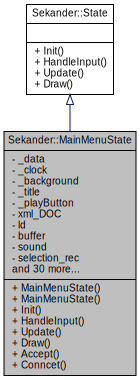
\includegraphics[width=212pt]{classSekander_1_1MainMenuState__inherit__graph}
\end{center}
\end{figure}


Collaboration diagram for Sekander\+:\+:Main\+Menu\+State\+:
\nopagebreak
\begin{figure}[H]
\begin{center}
\leavevmode
\includegraphics[height=550pt]{classSekander_1_1MainMenuState__coll__graph}
\end{center}
\end{figure}
\subsection*{Public Member Functions}
\begin{DoxyCompactItemize}
\item 
\hyperlink{classSekander_1_1MainMenuState_a6358c7103ad56cb05813567ab1d591ba}{Main\+Menu\+State} (\hyperlink{namespaceSekander_a1d69b002ba2d23020901c28f0def5e16}{Game\+Data\+Ref} data)
\item 
\hyperlink{classSekander_1_1MainMenuState_aeeea19d38e84e2ed002a4b47d6d8885e}{Main\+Menu\+State} (\hyperlink{namespaceSekander_a1d69b002ba2d23020901c28f0def5e16}{Game\+Data\+Ref} data, const char $\ast$\hyperlink{classSekander_1_1MainMenuState_ab1dafb7e7d50beb5418e72334f81dabd}{xml\+\_\+\+D\+OC})
\item 
void \hyperlink{classSekander_1_1MainMenuState_a45ea852b4aa57ee6c6204da1262c5e91}{Init} ()
\item 
void \hyperlink{classSekander_1_1MainMenuState_a960cd5207d1869e28d6388e267672397}{Handle\+Input} ()
\item 
void \hyperlink{classSekander_1_1MainMenuState_aabbfda236df88eee953e3b88ca8e7631}{Update} (float dt)
\item 
void \hyperlink{classSekander_1_1MainMenuState_a18aceffe0c53cf90263c24665de379c1}{Draw} (float dt)
\item 
void \hyperlink{classSekander_1_1MainMenuState_ab70a367c525cfb7bc8e0f5497c1159a9}{Accept} ()
\item 
void \hyperlink{classSekander_1_1MainMenuState_ab29df2f2392625cddc8c414f9a67a320}{Conncet} ()
\end{DoxyCompactItemize}
\subsection*{Private Attributes}
\begin{DoxyCompactItemize}
\item 
\hyperlink{namespaceSekander_a1d69b002ba2d23020901c28f0def5e16}{Game\+Data\+Ref} \hyperlink{classSekander_1_1MainMenuState_a531c88f2e6cc0645a0884a838c821ebc}{\+\_\+data}
\item 
sf\+::\+Clock \hyperlink{classSekander_1_1MainMenuState_a6a325d1ce58ad153f8647cf415968e50}{\+\_\+clock}
\item 
sf\+::\+Sprite \hyperlink{classSekander_1_1MainMenuState_a4397a65b30ddc70f19fb7cb5eef95b40}{\+\_\+background}
\item 
sf\+::\+Sprite \hyperlink{classSekander_1_1MainMenuState_ab8a4eec1c1100bed373e648a0659d26c}{\+\_\+title}
\item 
sf\+::\+Sprite \hyperlink{classSekander_1_1MainMenuState_a0283163c03392b1f056e682885822568}{\+\_\+play\+Button}
\item 
const char $\ast$ \hyperlink{classSekander_1_1MainMenuState_ab1dafb7e7d50beb5418e72334f81dabd}{xml\+\_\+\+D\+OC}
\item 
\hyperlink{classSekander_1_1LoadingGameObjects}{Loading\+Game\+Objects} $\ast$ \hyperlink{classSekander_1_1MainMenuState_ac0847b104c1fcbfcf19c9216b453d34c}{ld}
\item 
sf\+::\+Sound\+Buffer \hyperlink{classSekander_1_1MainMenuState_a9e445190379faaf2b2f7f8a97f55204d}{buffer}
\item 
sf\+::\+Sound \hyperlink{classSekander_1_1MainMenuState_af764062a7f43fc388d4e687ab3dca3e5}{sound}
\item 
sf\+::\+Rectangle\+Shape \hyperlink{classSekander_1_1MainMenuState_afa67fe296f512954d3c571e2c238ebd0}{selection\+\_\+rec}
\item 
int \hyperlink{classSekander_1_1MainMenuState_aca590f1c1e91223e5f783a93592f165c}{r} = 100
\item 
int \hyperlink{classSekander_1_1MainMenuState_a8e13c8df7da479728bef75e72cf4fb29}{b} = 255
\item 
int \hyperlink{classSekander_1_1MainMenuState_a8ee331bec9e89dcc67d231cf1c04bd83}{g} = 0
\item 
short int \hyperlink{classSekander_1_1MainMenuState_a8f65f83c7db9e9daae0aa0895f462367}{counter} = 0
\item 
bool \hyperlink{classSekander_1_1MainMenuState_a1a25539301721a9ee12f71309d5a62f1}{play\+\_\+button}
\item 
bool \hyperlink{classSekander_1_1MainMenuState_a5ebf1c8d29ebdea2c6f527e0f37929c1}{seting\+\_\+button}
\item 
bool \hyperlink{classSekander_1_1MainMenuState_a96d6929e4627393d278b955fd1de5d33}{exit\+\_\+button}
\item 
sf\+::\+Tcp\+Socket $\ast$ \hyperlink{classSekander_1_1MainMenuState_a3f5905df121c601a8e818d2eab62ba6b}{socket}
\item 
sf\+::\+Tcp\+Socket $\ast$ \hyperlink{classSekander_1_1MainMenuState_a62fcd2f99962a03992e2858dc4765d89}{client}
\item 
std\+::vector$<$ sf\+::\+Tcp\+Socket $\ast$ $>$ \hyperlink{classSekander_1_1MainMenuState_a7159a331d12d28479ee65786f7c93bc1}{socket\+\_\+list}
\item 
bool \hyperlink{classSekander_1_1MainMenuState_a3162344a57f59cc489ed9caba2863bf1}{\+\_\+host} = false
\item 
bool \hyperlink{classSekander_1_1MainMenuState_aee9956c65e169ef75ccb46022d4785cb}{\+\_\+connect} = false
\item 
bool \hyperlink{classSekander_1_1MainMenuState_a32c8906cd8fadf7605bcda2179d2c19f}{i\+\_\+am\+\_\+the\+\_\+host} = false
\item 
bool \hyperlink{classSekander_1_1MainMenuState_ac844479292f860e487a2b24d447dd6dc}{i\+\_\+am\+\_\+the\+\_\+client} = false
\item 
bool \hyperlink{classSekander_1_1MainMenuState_ab8863f0722718dd1331d7f5a11c0a5fe}{established\+\_\+connection} = false
\item 
double \hyperlink{classSekander_1_1MainMenuState_afe1fb61b370c0c2e437af904d2529012}{two\+\_\+\+PI}
\item 
double \hyperlink{classSekander_1_1MainMenuState_ac958e893ea737c7940d313d6c85d4f97}{amplitude} = 200
\item 
int \hyperlink{classSekander_1_1MainMenuState_ad598c82514f10a946507387748488e92}{frequency} = 1
\item 
int \hyperlink{classSekander_1_1MainMenuState_a0ecd1f7e9110bd75c802497ff59e2220}{k} = 0
\item 
double \hyperlink{classSekander_1_1MainMenuState_a863c7ceaeacacb0176b025aacc2ac4dc}{y}
\item 
double \hyperlink{classSekander_1_1MainMenuState_a8f252e97a1df6804381dd900ec16d9ba}{x}
\item 
double \hyperlink{classSekander_1_1MainMenuState_a66dfd5262c9d2248e4dd4028b4a1b59e}{h} = 1
\item 
int \hyperlink{classSekander_1_1MainMenuState_a31a95c62e0539845388ac18d68c51098}{n\+\_\+point} = 1000
\item 
sf\+::\+Rectangle\+Shape \hyperlink{classSekander_1_1MainMenuState_ab4bc4a5922ecc10449370f3e7fa94d47}{window\+\_\+rec}
\item 
sf\+::\+Rectangle\+Shape \hyperlink{classSekander_1_1MainMenuState_a9e090e4993c718debc56945b2921b751}{window\+\_\+rec2}
\item 
int \hyperlink{classSekander_1_1MainMenuState_aa371caf0a47f5f6423236d0d33cccf22}{a} = 255
\item 
int \hyperlink{classSekander_1_1MainMenuState_a6325eb8b3d56ee143f033ea897ff9bbd}{a\+\_\+b} = 0
\item 
bool \hyperlink{classSekander_1_1MainMenuState_acea6e58d065065f4bc83b27f8b082a13}{\+\_\+max}
\item 
bool \hyperlink{classSekander_1_1MainMenuState_a186148721efc437af0da39d75ebe00c3}{fade\+\_\+out}
\item 
bool \hyperlink{classSekander_1_1MainMenuState_ad0b61501d7825abab5207f3eb83c7196}{connection\+\_\+established} = false
\end{DoxyCompactItemize}


\subsection{Constructor \& Destructor Documentation}
\mbox{\Hypertarget{classSekander_1_1MainMenuState_a6358c7103ad56cb05813567ab1d591ba}\label{classSekander_1_1MainMenuState_a6358c7103ad56cb05813567ab1d591ba}} 
\index{Sekander\+::\+Main\+Menu\+State@{Sekander\+::\+Main\+Menu\+State}!Main\+Menu\+State@{Main\+Menu\+State}}
\index{Main\+Menu\+State@{Main\+Menu\+State}!Sekander\+::\+Main\+Menu\+State@{Sekander\+::\+Main\+Menu\+State}}
\subsubsection{\texorpdfstring{Main\+Menu\+State()}{MainMenuState()}\hspace{0.1cm}{\footnotesize\ttfamily [1/2]}}
{\footnotesize\ttfamily Sekander\+::\+Main\+Menu\+State\+::\+Main\+Menu\+State (\begin{DoxyParamCaption}\item[{\hyperlink{namespaceSekander_a1d69b002ba2d23020901c28f0def5e16}{Game\+Data\+Ref}}]{data }\end{DoxyParamCaption})}

\mbox{\Hypertarget{classSekander_1_1MainMenuState_aeeea19d38e84e2ed002a4b47d6d8885e}\label{classSekander_1_1MainMenuState_aeeea19d38e84e2ed002a4b47d6d8885e}} 
\index{Sekander\+::\+Main\+Menu\+State@{Sekander\+::\+Main\+Menu\+State}!Main\+Menu\+State@{Main\+Menu\+State}}
\index{Main\+Menu\+State@{Main\+Menu\+State}!Sekander\+::\+Main\+Menu\+State@{Sekander\+::\+Main\+Menu\+State}}
\subsubsection{\texorpdfstring{Main\+Menu\+State()}{MainMenuState()}\hspace{0.1cm}{\footnotesize\ttfamily [2/2]}}
{\footnotesize\ttfamily Sekander\+::\+Main\+Menu\+State\+::\+Main\+Menu\+State (\begin{DoxyParamCaption}\item[{\hyperlink{namespaceSekander_a1d69b002ba2d23020901c28f0def5e16}{Game\+Data\+Ref}}]{data,  }\item[{const char $\ast$}]{xml\+\_\+\+D\+OC }\end{DoxyParamCaption})}



\subsection{Member Function Documentation}
\mbox{\Hypertarget{classSekander_1_1MainMenuState_ab70a367c525cfb7bc8e0f5497c1159a9}\label{classSekander_1_1MainMenuState_ab70a367c525cfb7bc8e0f5497c1159a9}} 
\index{Sekander\+::\+Main\+Menu\+State@{Sekander\+::\+Main\+Menu\+State}!Accept@{Accept}}
\index{Accept@{Accept}!Sekander\+::\+Main\+Menu\+State@{Sekander\+::\+Main\+Menu\+State}}
\subsubsection{\texorpdfstring{Accept()}{Accept()}}
{\footnotesize\ttfamily void Sekander\+::\+Main\+Menu\+State\+::\+Accept (\begin{DoxyParamCaption}{ }\end{DoxyParamCaption})\hspace{0.3cm}{\ttfamily [inline]}}

\mbox{\Hypertarget{classSekander_1_1MainMenuState_ab29df2f2392625cddc8c414f9a67a320}\label{classSekander_1_1MainMenuState_ab29df2f2392625cddc8c414f9a67a320}} 
\index{Sekander\+::\+Main\+Menu\+State@{Sekander\+::\+Main\+Menu\+State}!Conncet@{Conncet}}
\index{Conncet@{Conncet}!Sekander\+::\+Main\+Menu\+State@{Sekander\+::\+Main\+Menu\+State}}
\subsubsection{\texorpdfstring{Conncet()}{Conncet()}}
{\footnotesize\ttfamily void Sekander\+::\+Main\+Menu\+State\+::\+Conncet (\begin{DoxyParamCaption}{ }\end{DoxyParamCaption})\hspace{0.3cm}{\ttfamily [inline]}}

\mbox{\Hypertarget{classSekander_1_1MainMenuState_a18aceffe0c53cf90263c24665de379c1}\label{classSekander_1_1MainMenuState_a18aceffe0c53cf90263c24665de379c1}} 
\index{Sekander\+::\+Main\+Menu\+State@{Sekander\+::\+Main\+Menu\+State}!Draw@{Draw}}
\index{Draw@{Draw}!Sekander\+::\+Main\+Menu\+State@{Sekander\+::\+Main\+Menu\+State}}
\subsubsection{\texorpdfstring{Draw()}{Draw()}}
{\footnotesize\ttfamily void Sekander\+::\+Main\+Menu\+State\+::\+Draw (\begin{DoxyParamCaption}\item[{float}]{dt }\end{DoxyParamCaption})\hspace{0.3cm}{\ttfamily [virtual]}}



Implements \hyperlink{classSekander_1_1State_a6ae7c2de1985461232a3ad694ca736b5}{Sekander\+::\+State}.

\mbox{\Hypertarget{classSekander_1_1MainMenuState_a960cd5207d1869e28d6388e267672397}\label{classSekander_1_1MainMenuState_a960cd5207d1869e28d6388e267672397}} 
\index{Sekander\+::\+Main\+Menu\+State@{Sekander\+::\+Main\+Menu\+State}!Handle\+Input@{Handle\+Input}}
\index{Handle\+Input@{Handle\+Input}!Sekander\+::\+Main\+Menu\+State@{Sekander\+::\+Main\+Menu\+State}}
\subsubsection{\texorpdfstring{Handle\+Input()}{HandleInput()}}
{\footnotesize\ttfamily void Sekander\+::\+Main\+Menu\+State\+::\+Handle\+Input (\begin{DoxyParamCaption}{ }\end{DoxyParamCaption})\hspace{0.3cm}{\ttfamily [virtual]}}



Implements \hyperlink{classSekander_1_1State_ad55ae42f5887db5745fda9f2bd30aaa3}{Sekander\+::\+State}.

\mbox{\Hypertarget{classSekander_1_1MainMenuState_a45ea852b4aa57ee6c6204da1262c5e91}\label{classSekander_1_1MainMenuState_a45ea852b4aa57ee6c6204da1262c5e91}} 
\index{Sekander\+::\+Main\+Menu\+State@{Sekander\+::\+Main\+Menu\+State}!Init@{Init}}
\index{Init@{Init}!Sekander\+::\+Main\+Menu\+State@{Sekander\+::\+Main\+Menu\+State}}
\subsubsection{\texorpdfstring{Init()}{Init()}}
{\footnotesize\ttfamily void Sekander\+::\+Main\+Menu\+State\+::\+Init (\begin{DoxyParamCaption}{ }\end{DoxyParamCaption})\hspace{0.3cm}{\ttfamily [virtual]}}



Implements \hyperlink{classSekander_1_1State_a171be4b77d4c13e01849b867bd3fa8f5}{Sekander\+::\+State}.

\mbox{\Hypertarget{classSekander_1_1MainMenuState_aabbfda236df88eee953e3b88ca8e7631}\label{classSekander_1_1MainMenuState_aabbfda236df88eee953e3b88ca8e7631}} 
\index{Sekander\+::\+Main\+Menu\+State@{Sekander\+::\+Main\+Menu\+State}!Update@{Update}}
\index{Update@{Update}!Sekander\+::\+Main\+Menu\+State@{Sekander\+::\+Main\+Menu\+State}}
\subsubsection{\texorpdfstring{Update()}{Update()}}
{\footnotesize\ttfamily void Sekander\+::\+Main\+Menu\+State\+::\+Update (\begin{DoxyParamCaption}\item[{float}]{dt }\end{DoxyParamCaption})\hspace{0.3cm}{\ttfamily [virtual]}}



Implements \hyperlink{classSekander_1_1State_a08d49e399db6f68247f410f7fddc7963}{Sekander\+::\+State}.



\subsection{Member Data Documentation}
\mbox{\Hypertarget{classSekander_1_1MainMenuState_a4397a65b30ddc70f19fb7cb5eef95b40}\label{classSekander_1_1MainMenuState_a4397a65b30ddc70f19fb7cb5eef95b40}} 
\index{Sekander\+::\+Main\+Menu\+State@{Sekander\+::\+Main\+Menu\+State}!\+\_\+background@{\+\_\+background}}
\index{\+\_\+background@{\+\_\+background}!Sekander\+::\+Main\+Menu\+State@{Sekander\+::\+Main\+Menu\+State}}
\subsubsection{\texorpdfstring{\+\_\+background}{\_background}}
{\footnotesize\ttfamily sf\+::\+Sprite Sekander\+::\+Main\+Menu\+State\+::\+\_\+background\hspace{0.3cm}{\ttfamily [private]}}

\mbox{\Hypertarget{classSekander_1_1MainMenuState_a6a325d1ce58ad153f8647cf415968e50}\label{classSekander_1_1MainMenuState_a6a325d1ce58ad153f8647cf415968e50}} 
\index{Sekander\+::\+Main\+Menu\+State@{Sekander\+::\+Main\+Menu\+State}!\+\_\+clock@{\+\_\+clock}}
\index{\+\_\+clock@{\+\_\+clock}!Sekander\+::\+Main\+Menu\+State@{Sekander\+::\+Main\+Menu\+State}}
\subsubsection{\texorpdfstring{\+\_\+clock}{\_clock}}
{\footnotesize\ttfamily sf\+::\+Clock Sekander\+::\+Main\+Menu\+State\+::\+\_\+clock\hspace{0.3cm}{\ttfamily [private]}}

\mbox{\Hypertarget{classSekander_1_1MainMenuState_aee9956c65e169ef75ccb46022d4785cb}\label{classSekander_1_1MainMenuState_aee9956c65e169ef75ccb46022d4785cb}} 
\index{Sekander\+::\+Main\+Menu\+State@{Sekander\+::\+Main\+Menu\+State}!\+\_\+connect@{\+\_\+connect}}
\index{\+\_\+connect@{\+\_\+connect}!Sekander\+::\+Main\+Menu\+State@{Sekander\+::\+Main\+Menu\+State}}
\subsubsection{\texorpdfstring{\+\_\+connect}{\_connect}}
{\footnotesize\ttfamily bool Sekander\+::\+Main\+Menu\+State\+::\+\_\+connect = false\hspace{0.3cm}{\ttfamily [private]}}

\mbox{\Hypertarget{classSekander_1_1MainMenuState_a531c88f2e6cc0645a0884a838c821ebc}\label{classSekander_1_1MainMenuState_a531c88f2e6cc0645a0884a838c821ebc}} 
\index{Sekander\+::\+Main\+Menu\+State@{Sekander\+::\+Main\+Menu\+State}!\+\_\+data@{\+\_\+data}}
\index{\+\_\+data@{\+\_\+data}!Sekander\+::\+Main\+Menu\+State@{Sekander\+::\+Main\+Menu\+State}}
\subsubsection{\texorpdfstring{\+\_\+data}{\_data}}
{\footnotesize\ttfamily \hyperlink{namespaceSekander_a1d69b002ba2d23020901c28f0def5e16}{Game\+Data\+Ref} Sekander\+::\+Main\+Menu\+State\+::\+\_\+data\hspace{0.3cm}{\ttfamily [private]}}

\mbox{\Hypertarget{classSekander_1_1MainMenuState_a3162344a57f59cc489ed9caba2863bf1}\label{classSekander_1_1MainMenuState_a3162344a57f59cc489ed9caba2863bf1}} 
\index{Sekander\+::\+Main\+Menu\+State@{Sekander\+::\+Main\+Menu\+State}!\+\_\+host@{\+\_\+host}}
\index{\+\_\+host@{\+\_\+host}!Sekander\+::\+Main\+Menu\+State@{Sekander\+::\+Main\+Menu\+State}}
\subsubsection{\texorpdfstring{\+\_\+host}{\_host}}
{\footnotesize\ttfamily bool Sekander\+::\+Main\+Menu\+State\+::\+\_\+host = false\hspace{0.3cm}{\ttfamily [private]}}

\mbox{\Hypertarget{classSekander_1_1MainMenuState_acea6e58d065065f4bc83b27f8b082a13}\label{classSekander_1_1MainMenuState_acea6e58d065065f4bc83b27f8b082a13}} 
\index{Sekander\+::\+Main\+Menu\+State@{Sekander\+::\+Main\+Menu\+State}!\+\_\+max@{\+\_\+max}}
\index{\+\_\+max@{\+\_\+max}!Sekander\+::\+Main\+Menu\+State@{Sekander\+::\+Main\+Menu\+State}}
\subsubsection{\texorpdfstring{\+\_\+max}{\_max}}
{\footnotesize\ttfamily bool Sekander\+::\+Main\+Menu\+State\+::\+\_\+max\hspace{0.3cm}{\ttfamily [private]}}

\mbox{\Hypertarget{classSekander_1_1MainMenuState_a0283163c03392b1f056e682885822568}\label{classSekander_1_1MainMenuState_a0283163c03392b1f056e682885822568}} 
\index{Sekander\+::\+Main\+Menu\+State@{Sekander\+::\+Main\+Menu\+State}!\+\_\+play\+Button@{\+\_\+play\+Button}}
\index{\+\_\+play\+Button@{\+\_\+play\+Button}!Sekander\+::\+Main\+Menu\+State@{Sekander\+::\+Main\+Menu\+State}}
\subsubsection{\texorpdfstring{\+\_\+play\+Button}{\_playButton}}
{\footnotesize\ttfamily sf\+::\+Sprite Sekander\+::\+Main\+Menu\+State\+::\+\_\+play\+Button\hspace{0.3cm}{\ttfamily [private]}}

\mbox{\Hypertarget{classSekander_1_1MainMenuState_ab8a4eec1c1100bed373e648a0659d26c}\label{classSekander_1_1MainMenuState_ab8a4eec1c1100bed373e648a0659d26c}} 
\index{Sekander\+::\+Main\+Menu\+State@{Sekander\+::\+Main\+Menu\+State}!\+\_\+title@{\+\_\+title}}
\index{\+\_\+title@{\+\_\+title}!Sekander\+::\+Main\+Menu\+State@{Sekander\+::\+Main\+Menu\+State}}
\subsubsection{\texorpdfstring{\+\_\+title}{\_title}}
{\footnotesize\ttfamily sf\+::\+Sprite Sekander\+::\+Main\+Menu\+State\+::\+\_\+title\hspace{0.3cm}{\ttfamily [private]}}

\mbox{\Hypertarget{classSekander_1_1MainMenuState_aa371caf0a47f5f6423236d0d33cccf22}\label{classSekander_1_1MainMenuState_aa371caf0a47f5f6423236d0d33cccf22}} 
\index{Sekander\+::\+Main\+Menu\+State@{Sekander\+::\+Main\+Menu\+State}!a@{a}}
\index{a@{a}!Sekander\+::\+Main\+Menu\+State@{Sekander\+::\+Main\+Menu\+State}}
\subsubsection{\texorpdfstring{a}{a}}
{\footnotesize\ttfamily int Sekander\+::\+Main\+Menu\+State\+::a = 255\hspace{0.3cm}{\ttfamily [private]}}

\mbox{\Hypertarget{classSekander_1_1MainMenuState_a6325eb8b3d56ee143f033ea897ff9bbd}\label{classSekander_1_1MainMenuState_a6325eb8b3d56ee143f033ea897ff9bbd}} 
\index{Sekander\+::\+Main\+Menu\+State@{Sekander\+::\+Main\+Menu\+State}!a\+\_\+b@{a\+\_\+b}}
\index{a\+\_\+b@{a\+\_\+b}!Sekander\+::\+Main\+Menu\+State@{Sekander\+::\+Main\+Menu\+State}}
\subsubsection{\texorpdfstring{a\+\_\+b}{a\_b}}
{\footnotesize\ttfamily int Sekander\+::\+Main\+Menu\+State\+::a\+\_\+b = 0\hspace{0.3cm}{\ttfamily [private]}}

\mbox{\Hypertarget{classSekander_1_1MainMenuState_ac958e893ea737c7940d313d6c85d4f97}\label{classSekander_1_1MainMenuState_ac958e893ea737c7940d313d6c85d4f97}} 
\index{Sekander\+::\+Main\+Menu\+State@{Sekander\+::\+Main\+Menu\+State}!amplitude@{amplitude}}
\index{amplitude@{amplitude}!Sekander\+::\+Main\+Menu\+State@{Sekander\+::\+Main\+Menu\+State}}
\subsubsection{\texorpdfstring{amplitude}{amplitude}}
{\footnotesize\ttfamily double Sekander\+::\+Main\+Menu\+State\+::amplitude = 200\hspace{0.3cm}{\ttfamily [private]}}

\mbox{\Hypertarget{classSekander_1_1MainMenuState_a8e13c8df7da479728bef75e72cf4fb29}\label{classSekander_1_1MainMenuState_a8e13c8df7da479728bef75e72cf4fb29}} 
\index{Sekander\+::\+Main\+Menu\+State@{Sekander\+::\+Main\+Menu\+State}!b@{b}}
\index{b@{b}!Sekander\+::\+Main\+Menu\+State@{Sekander\+::\+Main\+Menu\+State}}
\subsubsection{\texorpdfstring{b}{b}}
{\footnotesize\ttfamily int Sekander\+::\+Main\+Menu\+State\+::b = 255\hspace{0.3cm}{\ttfamily [private]}}

\mbox{\Hypertarget{classSekander_1_1MainMenuState_a9e445190379faaf2b2f7f8a97f55204d}\label{classSekander_1_1MainMenuState_a9e445190379faaf2b2f7f8a97f55204d}} 
\index{Sekander\+::\+Main\+Menu\+State@{Sekander\+::\+Main\+Menu\+State}!buffer@{buffer}}
\index{buffer@{buffer}!Sekander\+::\+Main\+Menu\+State@{Sekander\+::\+Main\+Menu\+State}}
\subsubsection{\texorpdfstring{buffer}{buffer}}
{\footnotesize\ttfamily sf\+::\+Sound\+Buffer Sekander\+::\+Main\+Menu\+State\+::buffer\hspace{0.3cm}{\ttfamily [private]}}

\mbox{\Hypertarget{classSekander_1_1MainMenuState_a62fcd2f99962a03992e2858dc4765d89}\label{classSekander_1_1MainMenuState_a62fcd2f99962a03992e2858dc4765d89}} 
\index{Sekander\+::\+Main\+Menu\+State@{Sekander\+::\+Main\+Menu\+State}!client@{client}}
\index{client@{client}!Sekander\+::\+Main\+Menu\+State@{Sekander\+::\+Main\+Menu\+State}}
\subsubsection{\texorpdfstring{client}{client}}
{\footnotesize\ttfamily sf\+::\+Tcp\+Socket$\ast$ Sekander\+::\+Main\+Menu\+State\+::client\hspace{0.3cm}{\ttfamily [private]}}

\mbox{\Hypertarget{classSekander_1_1MainMenuState_ad0b61501d7825abab5207f3eb83c7196}\label{classSekander_1_1MainMenuState_ad0b61501d7825abab5207f3eb83c7196}} 
\index{Sekander\+::\+Main\+Menu\+State@{Sekander\+::\+Main\+Menu\+State}!connection\+\_\+established@{connection\+\_\+established}}
\index{connection\+\_\+established@{connection\+\_\+established}!Sekander\+::\+Main\+Menu\+State@{Sekander\+::\+Main\+Menu\+State}}
\subsubsection{\texorpdfstring{connection\+\_\+established}{connection\_established}}
{\footnotesize\ttfamily bool Sekander\+::\+Main\+Menu\+State\+::connection\+\_\+established = false\hspace{0.3cm}{\ttfamily [private]}}

\mbox{\Hypertarget{classSekander_1_1MainMenuState_a8f65f83c7db9e9daae0aa0895f462367}\label{classSekander_1_1MainMenuState_a8f65f83c7db9e9daae0aa0895f462367}} 
\index{Sekander\+::\+Main\+Menu\+State@{Sekander\+::\+Main\+Menu\+State}!counter@{counter}}
\index{counter@{counter}!Sekander\+::\+Main\+Menu\+State@{Sekander\+::\+Main\+Menu\+State}}
\subsubsection{\texorpdfstring{counter}{counter}}
{\footnotesize\ttfamily short int Sekander\+::\+Main\+Menu\+State\+::counter = 0\hspace{0.3cm}{\ttfamily [private]}}

\mbox{\Hypertarget{classSekander_1_1MainMenuState_ab8863f0722718dd1331d7f5a11c0a5fe}\label{classSekander_1_1MainMenuState_ab8863f0722718dd1331d7f5a11c0a5fe}} 
\index{Sekander\+::\+Main\+Menu\+State@{Sekander\+::\+Main\+Menu\+State}!established\+\_\+connection@{established\+\_\+connection}}
\index{established\+\_\+connection@{established\+\_\+connection}!Sekander\+::\+Main\+Menu\+State@{Sekander\+::\+Main\+Menu\+State}}
\subsubsection{\texorpdfstring{established\+\_\+connection}{established\_connection}}
{\footnotesize\ttfamily bool Sekander\+::\+Main\+Menu\+State\+::established\+\_\+connection = false\hspace{0.3cm}{\ttfamily [private]}}

\mbox{\Hypertarget{classSekander_1_1MainMenuState_a96d6929e4627393d278b955fd1de5d33}\label{classSekander_1_1MainMenuState_a96d6929e4627393d278b955fd1de5d33}} 
\index{Sekander\+::\+Main\+Menu\+State@{Sekander\+::\+Main\+Menu\+State}!exit\+\_\+button@{exit\+\_\+button}}
\index{exit\+\_\+button@{exit\+\_\+button}!Sekander\+::\+Main\+Menu\+State@{Sekander\+::\+Main\+Menu\+State}}
\subsubsection{\texorpdfstring{exit\+\_\+button}{exit\_button}}
{\footnotesize\ttfamily bool Sekander\+::\+Main\+Menu\+State\+::exit\+\_\+button\hspace{0.3cm}{\ttfamily [private]}}

\mbox{\Hypertarget{classSekander_1_1MainMenuState_a186148721efc437af0da39d75ebe00c3}\label{classSekander_1_1MainMenuState_a186148721efc437af0da39d75ebe00c3}} 
\index{Sekander\+::\+Main\+Menu\+State@{Sekander\+::\+Main\+Menu\+State}!fade\+\_\+out@{fade\+\_\+out}}
\index{fade\+\_\+out@{fade\+\_\+out}!Sekander\+::\+Main\+Menu\+State@{Sekander\+::\+Main\+Menu\+State}}
\subsubsection{\texorpdfstring{fade\+\_\+out}{fade\_out}}
{\footnotesize\ttfamily bool Sekander\+::\+Main\+Menu\+State\+::fade\+\_\+out\hspace{0.3cm}{\ttfamily [private]}}

\mbox{\Hypertarget{classSekander_1_1MainMenuState_ad598c82514f10a946507387748488e92}\label{classSekander_1_1MainMenuState_ad598c82514f10a946507387748488e92}} 
\index{Sekander\+::\+Main\+Menu\+State@{Sekander\+::\+Main\+Menu\+State}!frequency@{frequency}}
\index{frequency@{frequency}!Sekander\+::\+Main\+Menu\+State@{Sekander\+::\+Main\+Menu\+State}}
\subsubsection{\texorpdfstring{frequency}{frequency}}
{\footnotesize\ttfamily int Sekander\+::\+Main\+Menu\+State\+::frequency = 1\hspace{0.3cm}{\ttfamily [private]}}

\mbox{\Hypertarget{classSekander_1_1MainMenuState_a8ee331bec9e89dcc67d231cf1c04bd83}\label{classSekander_1_1MainMenuState_a8ee331bec9e89dcc67d231cf1c04bd83}} 
\index{Sekander\+::\+Main\+Menu\+State@{Sekander\+::\+Main\+Menu\+State}!g@{g}}
\index{g@{g}!Sekander\+::\+Main\+Menu\+State@{Sekander\+::\+Main\+Menu\+State}}
\subsubsection{\texorpdfstring{g}{g}}
{\footnotesize\ttfamily int Sekander\+::\+Main\+Menu\+State\+::g = 0\hspace{0.3cm}{\ttfamily [private]}}

\mbox{\Hypertarget{classSekander_1_1MainMenuState_a66dfd5262c9d2248e4dd4028b4a1b59e}\label{classSekander_1_1MainMenuState_a66dfd5262c9d2248e4dd4028b4a1b59e}} 
\index{Sekander\+::\+Main\+Menu\+State@{Sekander\+::\+Main\+Menu\+State}!h@{h}}
\index{h@{h}!Sekander\+::\+Main\+Menu\+State@{Sekander\+::\+Main\+Menu\+State}}
\subsubsection{\texorpdfstring{h}{h}}
{\footnotesize\ttfamily double Sekander\+::\+Main\+Menu\+State\+::h = 1\hspace{0.3cm}{\ttfamily [private]}}

\mbox{\Hypertarget{classSekander_1_1MainMenuState_ac844479292f860e487a2b24d447dd6dc}\label{classSekander_1_1MainMenuState_ac844479292f860e487a2b24d447dd6dc}} 
\index{Sekander\+::\+Main\+Menu\+State@{Sekander\+::\+Main\+Menu\+State}!i\+\_\+am\+\_\+the\+\_\+client@{i\+\_\+am\+\_\+the\+\_\+client}}
\index{i\+\_\+am\+\_\+the\+\_\+client@{i\+\_\+am\+\_\+the\+\_\+client}!Sekander\+::\+Main\+Menu\+State@{Sekander\+::\+Main\+Menu\+State}}
\subsubsection{\texorpdfstring{i\+\_\+am\+\_\+the\+\_\+client}{i\_am\_the\_client}}
{\footnotesize\ttfamily bool Sekander\+::\+Main\+Menu\+State\+::i\+\_\+am\+\_\+the\+\_\+client = false\hspace{0.3cm}{\ttfamily [private]}}

\mbox{\Hypertarget{classSekander_1_1MainMenuState_a32c8906cd8fadf7605bcda2179d2c19f}\label{classSekander_1_1MainMenuState_a32c8906cd8fadf7605bcda2179d2c19f}} 
\index{Sekander\+::\+Main\+Menu\+State@{Sekander\+::\+Main\+Menu\+State}!i\+\_\+am\+\_\+the\+\_\+host@{i\+\_\+am\+\_\+the\+\_\+host}}
\index{i\+\_\+am\+\_\+the\+\_\+host@{i\+\_\+am\+\_\+the\+\_\+host}!Sekander\+::\+Main\+Menu\+State@{Sekander\+::\+Main\+Menu\+State}}
\subsubsection{\texorpdfstring{i\+\_\+am\+\_\+the\+\_\+host}{i\_am\_the\_host}}
{\footnotesize\ttfamily bool Sekander\+::\+Main\+Menu\+State\+::i\+\_\+am\+\_\+the\+\_\+host = false\hspace{0.3cm}{\ttfamily [private]}}

\mbox{\Hypertarget{classSekander_1_1MainMenuState_a0ecd1f7e9110bd75c802497ff59e2220}\label{classSekander_1_1MainMenuState_a0ecd1f7e9110bd75c802497ff59e2220}} 
\index{Sekander\+::\+Main\+Menu\+State@{Sekander\+::\+Main\+Menu\+State}!k@{k}}
\index{k@{k}!Sekander\+::\+Main\+Menu\+State@{Sekander\+::\+Main\+Menu\+State}}
\subsubsection{\texorpdfstring{k}{k}}
{\footnotesize\ttfamily int Sekander\+::\+Main\+Menu\+State\+::k = 0\hspace{0.3cm}{\ttfamily [private]}}

\mbox{\Hypertarget{classSekander_1_1MainMenuState_ac0847b104c1fcbfcf19c9216b453d34c}\label{classSekander_1_1MainMenuState_ac0847b104c1fcbfcf19c9216b453d34c}} 
\index{Sekander\+::\+Main\+Menu\+State@{Sekander\+::\+Main\+Menu\+State}!ld@{ld}}
\index{ld@{ld}!Sekander\+::\+Main\+Menu\+State@{Sekander\+::\+Main\+Menu\+State}}
\subsubsection{\texorpdfstring{ld}{ld}}
{\footnotesize\ttfamily \hyperlink{classSekander_1_1LoadingGameObjects}{Loading\+Game\+Objects}$\ast$ Sekander\+::\+Main\+Menu\+State\+::ld\hspace{0.3cm}{\ttfamily [private]}}

\mbox{\Hypertarget{classSekander_1_1MainMenuState_a31a95c62e0539845388ac18d68c51098}\label{classSekander_1_1MainMenuState_a31a95c62e0539845388ac18d68c51098}} 
\index{Sekander\+::\+Main\+Menu\+State@{Sekander\+::\+Main\+Menu\+State}!n\+\_\+point@{n\+\_\+point}}
\index{n\+\_\+point@{n\+\_\+point}!Sekander\+::\+Main\+Menu\+State@{Sekander\+::\+Main\+Menu\+State}}
\subsubsection{\texorpdfstring{n\+\_\+point}{n\_point}}
{\footnotesize\ttfamily int Sekander\+::\+Main\+Menu\+State\+::n\+\_\+point = 1000\hspace{0.3cm}{\ttfamily [private]}}

\mbox{\Hypertarget{classSekander_1_1MainMenuState_a1a25539301721a9ee12f71309d5a62f1}\label{classSekander_1_1MainMenuState_a1a25539301721a9ee12f71309d5a62f1}} 
\index{Sekander\+::\+Main\+Menu\+State@{Sekander\+::\+Main\+Menu\+State}!play\+\_\+button@{play\+\_\+button}}
\index{play\+\_\+button@{play\+\_\+button}!Sekander\+::\+Main\+Menu\+State@{Sekander\+::\+Main\+Menu\+State}}
\subsubsection{\texorpdfstring{play\+\_\+button}{play\_button}}
{\footnotesize\ttfamily bool Sekander\+::\+Main\+Menu\+State\+::play\+\_\+button\hspace{0.3cm}{\ttfamily [private]}}

\mbox{\Hypertarget{classSekander_1_1MainMenuState_aca590f1c1e91223e5f783a93592f165c}\label{classSekander_1_1MainMenuState_aca590f1c1e91223e5f783a93592f165c}} 
\index{Sekander\+::\+Main\+Menu\+State@{Sekander\+::\+Main\+Menu\+State}!r@{r}}
\index{r@{r}!Sekander\+::\+Main\+Menu\+State@{Sekander\+::\+Main\+Menu\+State}}
\subsubsection{\texorpdfstring{r}{r}}
{\footnotesize\ttfamily int Sekander\+::\+Main\+Menu\+State\+::r = 100\hspace{0.3cm}{\ttfamily [private]}}

\mbox{\Hypertarget{classSekander_1_1MainMenuState_afa67fe296f512954d3c571e2c238ebd0}\label{classSekander_1_1MainMenuState_afa67fe296f512954d3c571e2c238ebd0}} 
\index{Sekander\+::\+Main\+Menu\+State@{Sekander\+::\+Main\+Menu\+State}!selection\+\_\+rec@{selection\+\_\+rec}}
\index{selection\+\_\+rec@{selection\+\_\+rec}!Sekander\+::\+Main\+Menu\+State@{Sekander\+::\+Main\+Menu\+State}}
\subsubsection{\texorpdfstring{selection\+\_\+rec}{selection\_rec}}
{\footnotesize\ttfamily sf\+::\+Rectangle\+Shape Sekander\+::\+Main\+Menu\+State\+::selection\+\_\+rec\hspace{0.3cm}{\ttfamily [private]}}

\mbox{\Hypertarget{classSekander_1_1MainMenuState_a5ebf1c8d29ebdea2c6f527e0f37929c1}\label{classSekander_1_1MainMenuState_a5ebf1c8d29ebdea2c6f527e0f37929c1}} 
\index{Sekander\+::\+Main\+Menu\+State@{Sekander\+::\+Main\+Menu\+State}!seting\+\_\+button@{seting\+\_\+button}}
\index{seting\+\_\+button@{seting\+\_\+button}!Sekander\+::\+Main\+Menu\+State@{Sekander\+::\+Main\+Menu\+State}}
\subsubsection{\texorpdfstring{seting\+\_\+button}{seting\_button}}
{\footnotesize\ttfamily bool Sekander\+::\+Main\+Menu\+State\+::seting\+\_\+button\hspace{0.3cm}{\ttfamily [private]}}

\mbox{\Hypertarget{classSekander_1_1MainMenuState_a3f5905df121c601a8e818d2eab62ba6b}\label{classSekander_1_1MainMenuState_a3f5905df121c601a8e818d2eab62ba6b}} 
\index{Sekander\+::\+Main\+Menu\+State@{Sekander\+::\+Main\+Menu\+State}!socket@{socket}}
\index{socket@{socket}!Sekander\+::\+Main\+Menu\+State@{Sekander\+::\+Main\+Menu\+State}}
\subsubsection{\texorpdfstring{socket}{socket}}
{\footnotesize\ttfamily sf\+::\+Tcp\+Socket$\ast$ Sekander\+::\+Main\+Menu\+State\+::socket\hspace{0.3cm}{\ttfamily [private]}}

\mbox{\Hypertarget{classSekander_1_1MainMenuState_a7159a331d12d28479ee65786f7c93bc1}\label{classSekander_1_1MainMenuState_a7159a331d12d28479ee65786f7c93bc1}} 
\index{Sekander\+::\+Main\+Menu\+State@{Sekander\+::\+Main\+Menu\+State}!socket\+\_\+list@{socket\+\_\+list}}
\index{socket\+\_\+list@{socket\+\_\+list}!Sekander\+::\+Main\+Menu\+State@{Sekander\+::\+Main\+Menu\+State}}
\subsubsection{\texorpdfstring{socket\+\_\+list}{socket\_list}}
{\footnotesize\ttfamily std\+::vector$<$sf\+::\+Tcp\+Socket$\ast$$>$ Sekander\+::\+Main\+Menu\+State\+::socket\+\_\+list\hspace{0.3cm}{\ttfamily [private]}}

\mbox{\Hypertarget{classSekander_1_1MainMenuState_af764062a7f43fc388d4e687ab3dca3e5}\label{classSekander_1_1MainMenuState_af764062a7f43fc388d4e687ab3dca3e5}} 
\index{Sekander\+::\+Main\+Menu\+State@{Sekander\+::\+Main\+Menu\+State}!sound@{sound}}
\index{sound@{sound}!Sekander\+::\+Main\+Menu\+State@{Sekander\+::\+Main\+Menu\+State}}
\subsubsection{\texorpdfstring{sound}{sound}}
{\footnotesize\ttfamily sf\+::\+Sound Sekander\+::\+Main\+Menu\+State\+::sound\hspace{0.3cm}{\ttfamily [private]}}

\mbox{\Hypertarget{classSekander_1_1MainMenuState_afe1fb61b370c0c2e437af904d2529012}\label{classSekander_1_1MainMenuState_afe1fb61b370c0c2e437af904d2529012}} 
\index{Sekander\+::\+Main\+Menu\+State@{Sekander\+::\+Main\+Menu\+State}!two\+\_\+\+PI@{two\+\_\+\+PI}}
\index{two\+\_\+\+PI@{two\+\_\+\+PI}!Sekander\+::\+Main\+Menu\+State@{Sekander\+::\+Main\+Menu\+State}}
\subsubsection{\texorpdfstring{two\+\_\+\+PI}{two\_PI}}
{\footnotesize\ttfamily double Sekander\+::\+Main\+Menu\+State\+::two\+\_\+\+PI\hspace{0.3cm}{\ttfamily [private]}}

\mbox{\Hypertarget{classSekander_1_1MainMenuState_ab4bc4a5922ecc10449370f3e7fa94d47}\label{classSekander_1_1MainMenuState_ab4bc4a5922ecc10449370f3e7fa94d47}} 
\index{Sekander\+::\+Main\+Menu\+State@{Sekander\+::\+Main\+Menu\+State}!window\+\_\+rec@{window\+\_\+rec}}
\index{window\+\_\+rec@{window\+\_\+rec}!Sekander\+::\+Main\+Menu\+State@{Sekander\+::\+Main\+Menu\+State}}
\subsubsection{\texorpdfstring{window\+\_\+rec}{window\_rec}}
{\footnotesize\ttfamily sf\+::\+Rectangle\+Shape Sekander\+::\+Main\+Menu\+State\+::window\+\_\+rec\hspace{0.3cm}{\ttfamily [private]}}

\mbox{\Hypertarget{classSekander_1_1MainMenuState_a9e090e4993c718debc56945b2921b751}\label{classSekander_1_1MainMenuState_a9e090e4993c718debc56945b2921b751}} 
\index{Sekander\+::\+Main\+Menu\+State@{Sekander\+::\+Main\+Menu\+State}!window\+\_\+rec2@{window\+\_\+rec2}}
\index{window\+\_\+rec2@{window\+\_\+rec2}!Sekander\+::\+Main\+Menu\+State@{Sekander\+::\+Main\+Menu\+State}}
\subsubsection{\texorpdfstring{window\+\_\+rec2}{window\_rec2}}
{\footnotesize\ttfamily sf\+::\+Rectangle\+Shape Sekander\+::\+Main\+Menu\+State\+::window\+\_\+rec2\hspace{0.3cm}{\ttfamily [private]}}

\mbox{\Hypertarget{classSekander_1_1MainMenuState_a8f252e97a1df6804381dd900ec16d9ba}\label{classSekander_1_1MainMenuState_a8f252e97a1df6804381dd900ec16d9ba}} 
\index{Sekander\+::\+Main\+Menu\+State@{Sekander\+::\+Main\+Menu\+State}!x@{x}}
\index{x@{x}!Sekander\+::\+Main\+Menu\+State@{Sekander\+::\+Main\+Menu\+State}}
\subsubsection{\texorpdfstring{x}{x}}
{\footnotesize\ttfamily double Sekander\+::\+Main\+Menu\+State\+::x\hspace{0.3cm}{\ttfamily [private]}}

\mbox{\Hypertarget{classSekander_1_1MainMenuState_ab1dafb7e7d50beb5418e72334f81dabd}\label{classSekander_1_1MainMenuState_ab1dafb7e7d50beb5418e72334f81dabd}} 
\index{Sekander\+::\+Main\+Menu\+State@{Sekander\+::\+Main\+Menu\+State}!xml\+\_\+\+D\+OC@{xml\+\_\+\+D\+OC}}
\index{xml\+\_\+\+D\+OC@{xml\+\_\+\+D\+OC}!Sekander\+::\+Main\+Menu\+State@{Sekander\+::\+Main\+Menu\+State}}
\subsubsection{\texorpdfstring{xml\+\_\+\+D\+OC}{xml\_DOC}}
{\footnotesize\ttfamily const char$\ast$ Sekander\+::\+Main\+Menu\+State\+::xml\+\_\+\+D\+OC\hspace{0.3cm}{\ttfamily [private]}}

\mbox{\Hypertarget{classSekander_1_1MainMenuState_a863c7ceaeacacb0176b025aacc2ac4dc}\label{classSekander_1_1MainMenuState_a863c7ceaeacacb0176b025aacc2ac4dc}} 
\index{Sekander\+::\+Main\+Menu\+State@{Sekander\+::\+Main\+Menu\+State}!y@{y}}
\index{y@{y}!Sekander\+::\+Main\+Menu\+State@{Sekander\+::\+Main\+Menu\+State}}
\subsubsection{\texorpdfstring{y}{y}}
{\footnotesize\ttfamily double Sekander\+::\+Main\+Menu\+State\+::y\hspace{0.3cm}{\ttfamily [private]}}



The documentation for this class was generated from the following files\+:\begin{DoxyCompactItemize}
\item 
/mnt/hdd/\+C0de/\+Engines/\+S\+F\+M\+L/\+S\+F\+M\+L\+\_\+\+Engine/include/\hyperlink{MainMenuState_8hpp}{Main\+Menu\+State.\+hpp}\item 
/mnt/hdd/\+C0de/\+Engines/\+S\+F\+M\+L/\+S\+F\+M\+L\+\_\+\+Engine/src/\hyperlink{MainMenuState_8cpp}{Main\+Menu\+State.\+cpp}\end{DoxyCompactItemize}

\hypertarget{classMapLayer}{}\section{Map\+Layer Class Reference}
\label{classMapLayer}\index{Map\+Layer@{Map\+Layer}}


{\ttfamily \#include $<$S\+F\+M\+L\+Orthogonal\+Layer.\+hpp$>$}



Inheritance diagram for Map\+Layer\+:
\nopagebreak
\begin{figure}[H]
\begin{center}
\leavevmode
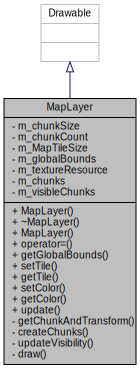
\includegraphics[width=212pt]{classMapLayer__inherit__graph}
\end{center}
\end{figure}


Collaboration diagram for Map\+Layer\+:
\nopagebreak
\begin{figure}[H]
\begin{center}
\leavevmode
\includegraphics[width=212pt]{classMapLayer__coll__graph}
\end{center}
\end{figure}
\subsection*{Classes}
\begin{DoxyCompactItemize}
\item 
struct \hyperlink{structMapLayer_1_1AnimationState}{Animation\+State}
\item 
class \hyperlink{classMapLayer_1_1Chunk}{Chunk}
\end{DoxyCompactItemize}
\subsection*{Public Member Functions}
\begin{DoxyCompactItemize}
\item 
\hyperlink{classMapLayer_ac1b9f1e3ba6d800abf508fa11490187b}{Map\+Layer} (const tmx\+::\+Map \&\hyperlink{classmap}{map}, std\+::size\+\_\+t idx)
\item 
\hyperlink{classMapLayer_a79858f9ee05242aa47ac680940e5ea74}{$\sim$\+Map\+Layer} ()=default
\item 
\hyperlink{classMapLayer_af323ddae8da169a64be1e0c216034397}{Map\+Layer} (const \hyperlink{classMapLayer}{Map\+Layer} \&)=delete
\item 
\hyperlink{classMapLayer}{Map\+Layer} \& \hyperlink{classMapLayer_a1863f3842c104aa6d460f4d9b99ec792}{operator=} (const \hyperlink{classMapLayer}{Map\+Layer} \&)=delete
\item 
const sf\+::\+Float\+Rect \& \hyperlink{classMapLayer_ae87bc38c7c030e9b2822b53f6de13d13}{get\+Global\+Bounds} () const
\item 
void \hyperlink{classMapLayer_a1152792435a0fa6203f6c3a038b93778}{set\+Tile} (int tileX, int tileY, tmx\+::\+Tile\+Layer\+::\+Tile tile, bool refresh=true)
\item 
tmx\+::\+Tile\+Layer\+::\+Tile \hyperlink{classMapLayer_a347375abb72832ea3362ba0d29898f30}{get\+Tile} (int tileX, int tileY)
\item 
void \hyperlink{classMapLayer_a4dad5e08a823925292846664ce42657d}{set\+Color} (int tileX, int tileY, sf\+::\+Color color, bool refresh=true)
\item 
sf\+::\+Color \hyperlink{classMapLayer_a6ecfbaf968ac9e6e4f814a30aa0c0f30}{get\+Color} (int tileX, int tileY)
\item 
void \hyperlink{classMapLayer_a0f7690e23ecfde7a7dc6629f9df65635}{update} (sf\+::\+Time elapsed)
\end{DoxyCompactItemize}
\subsection*{Private Types}
\begin{DoxyCompactItemize}
\item 
using \hyperlink{classMapLayer_a64011087426e436e3cb8374570378d68}{Texture\+Resource} = std\+::map$<$ std\+::string, std\+::unique\+\_\+ptr$<$ sf\+::\+Texture $>$ $>$
\end{DoxyCompactItemize}
\subsection*{Private Member Functions}
\begin{DoxyCompactItemize}
\item 
\hyperlink{classMapLayer_1_1Chunk_ab1df4d3621c5d9f83c2edb46d0744078}{Chunk\+::\+Ptr} \& \hyperlink{classMapLayer_a5686d500c087caa0c096c965d5d36574}{get\+Chunk\+And\+Transform} (int x, int y, sf\+::\+Vector2u \&chunk\+Relative)
\item 
void \hyperlink{classMapLayer_a853b2091fa76fabe4446797e0a01809a}{create\+Chunks} (const tmx\+::\+Map \&\hyperlink{classmap}{map}, const tmx\+::\+Tile\+Layer \&layer)
\item 
void \hyperlink{classMapLayer_a6602d1d89676fa73ace9934f7b77c0c5}{update\+Visibility} (const sf\+::\+View \&view) const
\item 
void \hyperlink{classMapLayer_a6a43405b98f14c3efbe02395c466c1e6}{draw} (sf\+::\+Render\+Target \&rt, sf\+::\+Render\+States states) const override
\end{DoxyCompactItemize}
\subsection*{Private Attributes}
\begin{DoxyCompactItemize}
\item 
sf\+::\+Vector2f \hyperlink{classMapLayer_af8d36b6ff112417b9d4f73a52e8859ae}{m\+\_\+chunk\+Size} = sf\+::\+Vector2f(512.f, 512.f)
\item 
sf\+::\+Vector2u \hyperlink{classMapLayer_ae816f79d9d81eb7e9e207c00bbf41218}{m\+\_\+chunk\+Count}
\item 
sf\+::\+Vector2u \hyperlink{classMapLayer_a9863689eb080d27e7a99dea7c20aee41}{m\+\_\+\+Map\+Tile\+Size}
\item 
sf\+::\+Float\+Rect \hyperlink{classMapLayer_a1e1ca5c4bedf393c1c85e2ced3bbf50a}{m\+\_\+global\+Bounds}
\item 
\hyperlink{classMapLayer_a64011087426e436e3cb8374570378d68}{Texture\+Resource} \hyperlink{classMapLayer_ad7cade67df5e55b3c6a960476e6d2cb9}{m\+\_\+texture\+Resource}
\item 
std\+::vector$<$ \hyperlink{classMapLayer_1_1Chunk_ab1df4d3621c5d9f83c2edb46d0744078}{Chunk\+::\+Ptr} $>$ \hyperlink{classMapLayer_a07e8acdbdfc63584a2b9276ca499ad70}{m\+\_\+chunks}
\item 
std\+::vector$<$ \hyperlink{classMapLayer_1_1Chunk}{Chunk} $\ast$ $>$ \hyperlink{classMapLayer_a74941b5479affea58ea8a3068770d430}{m\+\_\+visible\+Chunks}
\end{DoxyCompactItemize}


\subsection{Member Typedef Documentation}
\mbox{\Hypertarget{classMapLayer_a64011087426e436e3cb8374570378d68}\label{classMapLayer_a64011087426e436e3cb8374570378d68}} 
\index{Map\+Layer@{Map\+Layer}!Texture\+Resource@{Texture\+Resource}}
\index{Texture\+Resource@{Texture\+Resource}!Map\+Layer@{Map\+Layer}}
\subsubsection{\texorpdfstring{Texture\+Resource}{TextureResource}}
{\footnotesize\ttfamily using \hyperlink{classMapLayer_a64011087426e436e3cb8374570378d68}{Map\+Layer\+::\+Texture\+Resource} =  std\+::map$<$std\+::string, std\+::unique\+\_\+ptr$<$sf\+::\+Texture$>$ $>$\hspace{0.3cm}{\ttfamily [private]}}



\subsection{Constructor \& Destructor Documentation}
\mbox{\Hypertarget{classMapLayer_ac1b9f1e3ba6d800abf508fa11490187b}\label{classMapLayer_ac1b9f1e3ba6d800abf508fa11490187b}} 
\index{Map\+Layer@{Map\+Layer}!Map\+Layer@{Map\+Layer}}
\index{Map\+Layer@{Map\+Layer}!Map\+Layer@{Map\+Layer}}
\subsubsection{\texorpdfstring{Map\+Layer()}{MapLayer()}\hspace{0.1cm}{\footnotesize\ttfamily [1/2]}}
{\footnotesize\ttfamily Map\+Layer\+::\+Map\+Layer (\begin{DoxyParamCaption}\item[{const tmx\+::\+Map \&}]{map,  }\item[{std\+::size\+\_\+t}]{idx }\end{DoxyParamCaption})\hspace{0.3cm}{\ttfamily [inline]}}

\mbox{\Hypertarget{classMapLayer_a79858f9ee05242aa47ac680940e5ea74}\label{classMapLayer_a79858f9ee05242aa47ac680940e5ea74}} 
\index{Map\+Layer@{Map\+Layer}!````~Map\+Layer@{$\sim$\+Map\+Layer}}
\index{````~Map\+Layer@{$\sim$\+Map\+Layer}!Map\+Layer@{Map\+Layer}}
\subsubsection{\texorpdfstring{$\sim$\+Map\+Layer()}{~MapLayer()}}
{\footnotesize\ttfamily Map\+Layer\+::$\sim$\+Map\+Layer (\begin{DoxyParamCaption}{ }\end{DoxyParamCaption})\hspace{0.3cm}{\ttfamily [default]}}

\mbox{\Hypertarget{classMapLayer_af323ddae8da169a64be1e0c216034397}\label{classMapLayer_af323ddae8da169a64be1e0c216034397}} 
\index{Map\+Layer@{Map\+Layer}!Map\+Layer@{Map\+Layer}}
\index{Map\+Layer@{Map\+Layer}!Map\+Layer@{Map\+Layer}}
\subsubsection{\texorpdfstring{Map\+Layer()}{MapLayer()}\hspace{0.1cm}{\footnotesize\ttfamily [2/2]}}
{\footnotesize\ttfamily Map\+Layer\+::\+Map\+Layer (\begin{DoxyParamCaption}\item[{const \hyperlink{classMapLayer}{Map\+Layer} \&}]{ }\end{DoxyParamCaption})\hspace{0.3cm}{\ttfamily [delete]}}



\subsection{Member Function Documentation}
\mbox{\Hypertarget{classMapLayer_a853b2091fa76fabe4446797e0a01809a}\label{classMapLayer_a853b2091fa76fabe4446797e0a01809a}} 
\index{Map\+Layer@{Map\+Layer}!create\+Chunks@{create\+Chunks}}
\index{create\+Chunks@{create\+Chunks}!Map\+Layer@{Map\+Layer}}
\subsubsection{\texorpdfstring{create\+Chunks()}{createChunks()}}
{\footnotesize\ttfamily void Map\+Layer\+::create\+Chunks (\begin{DoxyParamCaption}\item[{const tmx\+::\+Map \&}]{map,  }\item[{const tmx\+::\+Tile\+Layer \&}]{layer }\end{DoxyParamCaption})\hspace{0.3cm}{\ttfamily [inline]}, {\ttfamily [private]}}

\mbox{\Hypertarget{classMapLayer_a6a43405b98f14c3efbe02395c466c1e6}\label{classMapLayer_a6a43405b98f14c3efbe02395c466c1e6}} 
\index{Map\+Layer@{Map\+Layer}!draw@{draw}}
\index{draw@{draw}!Map\+Layer@{Map\+Layer}}
\subsubsection{\texorpdfstring{draw()}{draw()}}
{\footnotesize\ttfamily void Map\+Layer\+::draw (\begin{DoxyParamCaption}\item[{sf\+::\+Render\+Target \&}]{rt,  }\item[{sf\+::\+Render\+States}]{states }\end{DoxyParamCaption}) const\hspace{0.3cm}{\ttfamily [inline]}, {\ttfamily [override]}, {\ttfamily [private]}}

\mbox{\Hypertarget{classMapLayer_a5686d500c087caa0c096c965d5d36574}\label{classMapLayer_a5686d500c087caa0c096c965d5d36574}} 
\index{Map\+Layer@{Map\+Layer}!get\+Chunk\+And\+Transform@{get\+Chunk\+And\+Transform}}
\index{get\+Chunk\+And\+Transform@{get\+Chunk\+And\+Transform}!Map\+Layer@{Map\+Layer}}
\subsubsection{\texorpdfstring{get\+Chunk\+And\+Transform()}{getChunkAndTransform()}}
{\footnotesize\ttfamily \hyperlink{classMapLayer_1_1Chunk_ab1df4d3621c5d9f83c2edb46d0744078}{Chunk\+::\+Ptr}\& Map\+Layer\+::get\+Chunk\+And\+Transform (\begin{DoxyParamCaption}\item[{int}]{x,  }\item[{int}]{y,  }\item[{sf\+::\+Vector2u \&}]{chunk\+Relative }\end{DoxyParamCaption})\hspace{0.3cm}{\ttfamily [inline]}, {\ttfamily [private]}}

\mbox{\Hypertarget{classMapLayer_a6ecfbaf968ac9e6e4f814a30aa0c0f30}\label{classMapLayer_a6ecfbaf968ac9e6e4f814a30aa0c0f30}} 
\index{Map\+Layer@{Map\+Layer}!get\+Color@{get\+Color}}
\index{get\+Color@{get\+Color}!Map\+Layer@{Map\+Layer}}
\subsubsection{\texorpdfstring{get\+Color()}{getColor()}}
{\footnotesize\ttfamily sf\+::\+Color Map\+Layer\+::get\+Color (\begin{DoxyParamCaption}\item[{int}]{tileX,  }\item[{int}]{tileY }\end{DoxyParamCaption})\hspace{0.3cm}{\ttfamily [inline]}}

\mbox{\Hypertarget{classMapLayer_ae87bc38c7c030e9b2822b53f6de13d13}\label{classMapLayer_ae87bc38c7c030e9b2822b53f6de13d13}} 
\index{Map\+Layer@{Map\+Layer}!get\+Global\+Bounds@{get\+Global\+Bounds}}
\index{get\+Global\+Bounds@{get\+Global\+Bounds}!Map\+Layer@{Map\+Layer}}
\subsubsection{\texorpdfstring{get\+Global\+Bounds()}{getGlobalBounds()}}
{\footnotesize\ttfamily const sf\+::\+Float\+Rect\& Map\+Layer\+::get\+Global\+Bounds (\begin{DoxyParamCaption}{ }\end{DoxyParamCaption}) const\hspace{0.3cm}{\ttfamily [inline]}}

\mbox{\Hypertarget{classMapLayer_a347375abb72832ea3362ba0d29898f30}\label{classMapLayer_a347375abb72832ea3362ba0d29898f30}} 
\index{Map\+Layer@{Map\+Layer}!get\+Tile@{get\+Tile}}
\index{get\+Tile@{get\+Tile}!Map\+Layer@{Map\+Layer}}
\subsubsection{\texorpdfstring{get\+Tile()}{getTile()}}
{\footnotesize\ttfamily tmx\+::\+Tile\+Layer\+::\+Tile Map\+Layer\+::get\+Tile (\begin{DoxyParamCaption}\item[{int}]{tileX,  }\item[{int}]{tileY }\end{DoxyParamCaption})\hspace{0.3cm}{\ttfamily [inline]}}

\mbox{\Hypertarget{classMapLayer_a1863f3842c104aa6d460f4d9b99ec792}\label{classMapLayer_a1863f3842c104aa6d460f4d9b99ec792}} 
\index{Map\+Layer@{Map\+Layer}!operator=@{operator=}}
\index{operator=@{operator=}!Map\+Layer@{Map\+Layer}}
\subsubsection{\texorpdfstring{operator=()}{operator=()}}
{\footnotesize\ttfamily \hyperlink{classMapLayer}{Map\+Layer}\& Map\+Layer\+::operator= (\begin{DoxyParamCaption}\item[{const \hyperlink{classMapLayer}{Map\+Layer} \&}]{ }\end{DoxyParamCaption})\hspace{0.3cm}{\ttfamily [delete]}}

\mbox{\Hypertarget{classMapLayer_a4dad5e08a823925292846664ce42657d}\label{classMapLayer_a4dad5e08a823925292846664ce42657d}} 
\index{Map\+Layer@{Map\+Layer}!set\+Color@{set\+Color}}
\index{set\+Color@{set\+Color}!Map\+Layer@{Map\+Layer}}
\subsubsection{\texorpdfstring{set\+Color()}{setColor()}}
{\footnotesize\ttfamily void Map\+Layer\+::set\+Color (\begin{DoxyParamCaption}\item[{int}]{tileX,  }\item[{int}]{tileY,  }\item[{sf\+::\+Color}]{color,  }\item[{bool}]{refresh = {\ttfamily true} }\end{DoxyParamCaption})\hspace{0.3cm}{\ttfamily [inline]}}

\mbox{\Hypertarget{classMapLayer_a1152792435a0fa6203f6c3a038b93778}\label{classMapLayer_a1152792435a0fa6203f6c3a038b93778}} 
\index{Map\+Layer@{Map\+Layer}!set\+Tile@{set\+Tile}}
\index{set\+Tile@{set\+Tile}!Map\+Layer@{Map\+Layer}}
\subsubsection{\texorpdfstring{set\+Tile()}{setTile()}}
{\footnotesize\ttfamily void Map\+Layer\+::set\+Tile (\begin{DoxyParamCaption}\item[{int}]{tileX,  }\item[{int}]{tileY,  }\item[{tmx\+::\+Tile\+Layer\+::\+Tile}]{tile,  }\item[{bool}]{refresh = {\ttfamily true} }\end{DoxyParamCaption})\hspace{0.3cm}{\ttfamily [inline]}}

\mbox{\Hypertarget{classMapLayer_a0f7690e23ecfde7a7dc6629f9df65635}\label{classMapLayer_a0f7690e23ecfde7a7dc6629f9df65635}} 
\index{Map\+Layer@{Map\+Layer}!update@{update}}
\index{update@{update}!Map\+Layer@{Map\+Layer}}
\subsubsection{\texorpdfstring{update()}{update()}}
{\footnotesize\ttfamily void Map\+Layer\+::update (\begin{DoxyParamCaption}\item[{sf\+::\+Time}]{elapsed }\end{DoxyParamCaption})\hspace{0.3cm}{\ttfamily [inline]}}

\mbox{\Hypertarget{classMapLayer_a6602d1d89676fa73ace9934f7b77c0c5}\label{classMapLayer_a6602d1d89676fa73ace9934f7b77c0c5}} 
\index{Map\+Layer@{Map\+Layer}!update\+Visibility@{update\+Visibility}}
\index{update\+Visibility@{update\+Visibility}!Map\+Layer@{Map\+Layer}}
\subsubsection{\texorpdfstring{update\+Visibility()}{updateVisibility()}}
{\footnotesize\ttfamily void Map\+Layer\+::update\+Visibility (\begin{DoxyParamCaption}\item[{const sf\+::\+View \&}]{view }\end{DoxyParamCaption}) const\hspace{0.3cm}{\ttfamily [inline]}, {\ttfamily [private]}}



\subsection{Member Data Documentation}
\mbox{\Hypertarget{classMapLayer_ae816f79d9d81eb7e9e207c00bbf41218}\label{classMapLayer_ae816f79d9d81eb7e9e207c00bbf41218}} 
\index{Map\+Layer@{Map\+Layer}!m\+\_\+chunk\+Count@{m\+\_\+chunk\+Count}}
\index{m\+\_\+chunk\+Count@{m\+\_\+chunk\+Count}!Map\+Layer@{Map\+Layer}}
\subsubsection{\texorpdfstring{m\+\_\+chunk\+Count}{m\_chunkCount}}
{\footnotesize\ttfamily sf\+::\+Vector2u Map\+Layer\+::m\+\_\+chunk\+Count\hspace{0.3cm}{\ttfamily [private]}}

\mbox{\Hypertarget{classMapLayer_a07e8acdbdfc63584a2b9276ca499ad70}\label{classMapLayer_a07e8acdbdfc63584a2b9276ca499ad70}} 
\index{Map\+Layer@{Map\+Layer}!m\+\_\+chunks@{m\+\_\+chunks}}
\index{m\+\_\+chunks@{m\+\_\+chunks}!Map\+Layer@{Map\+Layer}}
\subsubsection{\texorpdfstring{m\+\_\+chunks}{m\_chunks}}
{\footnotesize\ttfamily std\+::vector$<$\hyperlink{classMapLayer_1_1Chunk_ab1df4d3621c5d9f83c2edb46d0744078}{Chunk\+::\+Ptr}$>$ Map\+Layer\+::m\+\_\+chunks\hspace{0.3cm}{\ttfamily [private]}}

\mbox{\Hypertarget{classMapLayer_af8d36b6ff112417b9d4f73a52e8859ae}\label{classMapLayer_af8d36b6ff112417b9d4f73a52e8859ae}} 
\index{Map\+Layer@{Map\+Layer}!m\+\_\+chunk\+Size@{m\+\_\+chunk\+Size}}
\index{m\+\_\+chunk\+Size@{m\+\_\+chunk\+Size}!Map\+Layer@{Map\+Layer}}
\subsubsection{\texorpdfstring{m\+\_\+chunk\+Size}{m\_chunkSize}}
{\footnotesize\ttfamily sf\+::\+Vector2f Map\+Layer\+::m\+\_\+chunk\+Size = sf\+::\+Vector2f(512.f, 512.f)\hspace{0.3cm}{\ttfamily [private]}}

\mbox{\Hypertarget{classMapLayer_a1e1ca5c4bedf393c1c85e2ced3bbf50a}\label{classMapLayer_a1e1ca5c4bedf393c1c85e2ced3bbf50a}} 
\index{Map\+Layer@{Map\+Layer}!m\+\_\+global\+Bounds@{m\+\_\+global\+Bounds}}
\index{m\+\_\+global\+Bounds@{m\+\_\+global\+Bounds}!Map\+Layer@{Map\+Layer}}
\subsubsection{\texorpdfstring{m\+\_\+global\+Bounds}{m\_globalBounds}}
{\footnotesize\ttfamily sf\+::\+Float\+Rect Map\+Layer\+::m\+\_\+global\+Bounds\hspace{0.3cm}{\ttfamily [private]}}

\mbox{\Hypertarget{classMapLayer_a9863689eb080d27e7a99dea7c20aee41}\label{classMapLayer_a9863689eb080d27e7a99dea7c20aee41}} 
\index{Map\+Layer@{Map\+Layer}!m\+\_\+\+Map\+Tile\+Size@{m\+\_\+\+Map\+Tile\+Size}}
\index{m\+\_\+\+Map\+Tile\+Size@{m\+\_\+\+Map\+Tile\+Size}!Map\+Layer@{Map\+Layer}}
\subsubsection{\texorpdfstring{m\+\_\+\+Map\+Tile\+Size}{m\_MapTileSize}}
{\footnotesize\ttfamily sf\+::\+Vector2u Map\+Layer\+::m\+\_\+\+Map\+Tile\+Size\hspace{0.3cm}{\ttfamily [private]}}

\mbox{\Hypertarget{classMapLayer_ad7cade67df5e55b3c6a960476e6d2cb9}\label{classMapLayer_ad7cade67df5e55b3c6a960476e6d2cb9}} 
\index{Map\+Layer@{Map\+Layer}!m\+\_\+texture\+Resource@{m\+\_\+texture\+Resource}}
\index{m\+\_\+texture\+Resource@{m\+\_\+texture\+Resource}!Map\+Layer@{Map\+Layer}}
\subsubsection{\texorpdfstring{m\+\_\+texture\+Resource}{m\_textureResource}}
{\footnotesize\ttfamily \hyperlink{classMapLayer_a64011087426e436e3cb8374570378d68}{Texture\+Resource} Map\+Layer\+::m\+\_\+texture\+Resource\hspace{0.3cm}{\ttfamily [private]}}

\mbox{\Hypertarget{classMapLayer_a74941b5479affea58ea8a3068770d430}\label{classMapLayer_a74941b5479affea58ea8a3068770d430}} 
\index{Map\+Layer@{Map\+Layer}!m\+\_\+visible\+Chunks@{m\+\_\+visible\+Chunks}}
\index{m\+\_\+visible\+Chunks@{m\+\_\+visible\+Chunks}!Map\+Layer@{Map\+Layer}}
\subsubsection{\texorpdfstring{m\+\_\+visible\+Chunks}{m\_visibleChunks}}
{\footnotesize\ttfamily std\+::vector$<$\hyperlink{classMapLayer_1_1Chunk}{Chunk}$\ast$$>$ Map\+Layer\+::m\+\_\+visible\+Chunks\hspace{0.3cm}{\ttfamily [mutable]}, {\ttfamily [private]}}



The documentation for this class was generated from the following file\+:\begin{DoxyCompactItemize}
\item 
/mnt/hdd/\+C0de/smart\+\_\+engine/include/\hyperlink{SFMLOrthogonalLayer_8hpp}{S\+F\+M\+L\+Orthogonal\+Layer.\+hpp}\end{DoxyCompactItemize}

\hypertarget{classSekander_1_1SplashState}{}\section{Sekander\+:\+:Splash\+State Class Reference}
\label{classSekander_1_1SplashState}\index{Sekander\+::\+Splash\+State@{Sekander\+::\+Splash\+State}}


{\ttfamily \#include $<$Splash\+State.\+hpp$>$}



Inheritance diagram for Sekander\+:\+:Splash\+State\+:
\nopagebreak
\begin{figure}[H]
\begin{center}
\leavevmode
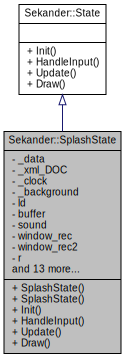
\includegraphics[width=197pt]{classSekander_1_1SplashState__inherit__graph}
\end{center}
\end{figure}


Collaboration diagram for Sekander\+:\+:Splash\+State\+:
\nopagebreak
\begin{figure}[H]
\begin{center}
\leavevmode
\includegraphics[height=550pt]{classSekander_1_1SplashState__coll__graph}
\end{center}
\end{figure}
\subsection*{Public Member Functions}
\begin{DoxyCompactItemize}
\item 
\hyperlink{classSekander_1_1SplashState_ae341ef8552453a1d343dcad68de101b5}{Splash\+State} (\hyperlink{namespaceSekander_a1d69b002ba2d23020901c28f0def5e16}{Game\+Data\+Ref} data)
\item 
\hyperlink{classSekander_1_1SplashState_aeb0bbd0553d10ed561166578b3fba993}{Splash\+State} (\hyperlink{namespaceSekander_a1d69b002ba2d23020901c28f0def5e16}{Game\+Data\+Ref} data, const char $\ast$xml\+\_\+\+D\+OC)
\item 
void \hyperlink{classSekander_1_1SplashState_adefc71fa2623180deda8391d4e64b04c}{Init} ()
\item 
void \hyperlink{classSekander_1_1SplashState_a70b45699149208c755d95d1ef3bdb202}{Handle\+Input} ()
\item 
void \hyperlink{classSekander_1_1SplashState_ac7121b90b97b7d9cdb5774bdc0c6cc2d}{Update} (float dt)
\item 
void \hyperlink{classSekander_1_1SplashState_ad372f3712cd5d3207e44a50dc70bed46}{Draw} (float dt)
\end{DoxyCompactItemize}
\subsection*{Private Attributes}
\begin{DoxyCompactItemize}
\item 
\hyperlink{namespaceSekander_a1d69b002ba2d23020901c28f0def5e16}{Game\+Data\+Ref} \hyperlink{classSekander_1_1SplashState_a9b4c437b8381b964f3888a9c34c505b3}{\+\_\+data}
\item 
const char $\ast$ \hyperlink{classSekander_1_1SplashState_a3b2a0dfe9948b7ce7b0090fd3a4d45ae}{\+\_\+xml\+\_\+\+D\+OC}
\item 
sf\+::\+Clock \hyperlink{classSekander_1_1SplashState_a536a6abd6bf7b25b13c643268e0cdc5f}{\+\_\+clock}
\item 
sf\+::\+Sprite \hyperlink{classSekander_1_1SplashState_a138c6168e7a3f910ec07e5358d885d5f}{\+\_\+background}
\item 
\hyperlink{classSekander_1_1LoadingGameObjects}{Loading\+Game\+Objects} $\ast$ \hyperlink{classSekander_1_1SplashState_a52b5e2e5c009568d86b8d04cab0f25eb}{ld}
\item 
sf\+::\+Sound\+Buffer \hyperlink{classSekander_1_1SplashState_ab55b67506296306d1052be850eee455b}{buffer}
\item 
sf\+::\+Sound \hyperlink{classSekander_1_1SplashState_a820828a38fcf1bafada569e889d5a779}{sound}
\item 
sf\+::\+Rectangle\+Shape \hyperlink{classSekander_1_1SplashState_a3522ebb11107475ddb6ab8b787b612b9}{window\+\_\+rec}
\item 
sf\+::\+Rectangle\+Shape \hyperlink{classSekander_1_1SplashState_a1f4bf1010fbec5d0873b465c9e8dec7d}{window\+\_\+rec2}
\item 
int \hyperlink{classSekander_1_1SplashState_a4d7ea7b0bddcdc29d96e08da7e2efbf4}{r} = 100
\item 
int \hyperlink{classSekander_1_1SplashState_aab2a67735fa67169f0359c9d788e6555}{b} = 100
\item 
int \hyperlink{classSekander_1_1SplashState_a20007b0dea253e377162ad99bd0e2c2b}{g} = 0
\item 
int \hyperlink{classSekander_1_1SplashState_a4afa8ff30b6f644d71009aaeacbef7cc}{a} = 255
\item 
int \hyperlink{classSekander_1_1SplashState_a71eb4ebad66f0d6b65d1aaac9dd394df}{a\+\_\+b} = 0
\item 
double \hyperlink{classSekander_1_1SplashState_a412b596a55aa117ae8b2ebc6c39450ec}{two\+\_\+\+PI}
\item 
double \hyperlink{classSekander_1_1SplashState_aad2e0b38cdf830b13e042c69cd2e758b}{amplitude} = 200
\item 
int \hyperlink{classSekander_1_1SplashState_a52681392f4d654d97af9504e8aa21aa0}{frequency} = 1
\item 
int \hyperlink{classSekander_1_1SplashState_a9442aa523cd10d3bbf8bc3da82b310c0}{k} = 0
\item 
double \hyperlink{classSekander_1_1SplashState_a6ae3a31d30343bb45aadef7966320668}{y}
\item 
double \hyperlink{classSekander_1_1SplashState_a5f21fde83d2389f995b64ab313716a09}{x}
\item 
double \hyperlink{classSekander_1_1SplashState_a98175bbd61d8dd4d74a813e5aada605d}{h} = 1
\item 
int \hyperlink{classSekander_1_1SplashState_a0d393d6f228cd011e23dcec4723f327a}{n\+\_\+point} = 1000
\item 
bool \hyperlink{classSekander_1_1SplashState_ae06ef54f8cd627aee5ca845eea105e0a}{\+\_\+max}
\end{DoxyCompactItemize}


\subsection{Constructor \& Destructor Documentation}
\mbox{\Hypertarget{classSekander_1_1SplashState_ae341ef8552453a1d343dcad68de101b5}\label{classSekander_1_1SplashState_ae341ef8552453a1d343dcad68de101b5}} 
\index{Sekander\+::\+Splash\+State@{Sekander\+::\+Splash\+State}!Splash\+State@{Splash\+State}}
\index{Splash\+State@{Splash\+State}!Sekander\+::\+Splash\+State@{Sekander\+::\+Splash\+State}}
\subsubsection{\texorpdfstring{Splash\+State()}{SplashState()}\hspace{0.1cm}{\footnotesize\ttfamily [1/2]}}
{\footnotesize\ttfamily Sekander\+::\+Splash\+State\+::\+Splash\+State (\begin{DoxyParamCaption}\item[{\hyperlink{namespaceSekander_a1d69b002ba2d23020901c28f0def5e16}{Game\+Data\+Ref}}]{data }\end{DoxyParamCaption})}

\mbox{\Hypertarget{classSekander_1_1SplashState_aeb0bbd0553d10ed561166578b3fba993}\label{classSekander_1_1SplashState_aeb0bbd0553d10ed561166578b3fba993}} 
\index{Sekander\+::\+Splash\+State@{Sekander\+::\+Splash\+State}!Splash\+State@{Splash\+State}}
\index{Splash\+State@{Splash\+State}!Sekander\+::\+Splash\+State@{Sekander\+::\+Splash\+State}}
\subsubsection{\texorpdfstring{Splash\+State()}{SplashState()}\hspace{0.1cm}{\footnotesize\ttfamily [2/2]}}
{\footnotesize\ttfamily Sekander\+::\+Splash\+State\+::\+Splash\+State (\begin{DoxyParamCaption}\item[{\hyperlink{namespaceSekander_a1d69b002ba2d23020901c28f0def5e16}{Game\+Data\+Ref}}]{data,  }\item[{const char $\ast$}]{xml\+\_\+\+D\+OC }\end{DoxyParamCaption})}



\subsection{Member Function Documentation}
\mbox{\Hypertarget{classSekander_1_1SplashState_ad372f3712cd5d3207e44a50dc70bed46}\label{classSekander_1_1SplashState_ad372f3712cd5d3207e44a50dc70bed46}} 
\index{Sekander\+::\+Splash\+State@{Sekander\+::\+Splash\+State}!Draw@{Draw}}
\index{Draw@{Draw}!Sekander\+::\+Splash\+State@{Sekander\+::\+Splash\+State}}
\subsubsection{\texorpdfstring{Draw()}{Draw()}}
{\footnotesize\ttfamily void Sekander\+::\+Splash\+State\+::\+Draw (\begin{DoxyParamCaption}\item[{float}]{dt }\end{DoxyParamCaption})\hspace{0.3cm}{\ttfamily [virtual]}}



Implements \hyperlink{classSekander_1_1State_a6ae7c2de1985461232a3ad694ca736b5}{Sekander\+::\+State}.

\mbox{\Hypertarget{classSekander_1_1SplashState_a70b45699149208c755d95d1ef3bdb202}\label{classSekander_1_1SplashState_a70b45699149208c755d95d1ef3bdb202}} 
\index{Sekander\+::\+Splash\+State@{Sekander\+::\+Splash\+State}!Handle\+Input@{Handle\+Input}}
\index{Handle\+Input@{Handle\+Input}!Sekander\+::\+Splash\+State@{Sekander\+::\+Splash\+State}}
\subsubsection{\texorpdfstring{Handle\+Input()}{HandleInput()}}
{\footnotesize\ttfamily void Sekander\+::\+Splash\+State\+::\+Handle\+Input (\begin{DoxyParamCaption}{ }\end{DoxyParamCaption})\hspace{0.3cm}{\ttfamily [virtual]}}



Implements \hyperlink{classSekander_1_1State_ad55ae42f5887db5745fda9f2bd30aaa3}{Sekander\+::\+State}.

\mbox{\Hypertarget{classSekander_1_1SplashState_adefc71fa2623180deda8391d4e64b04c}\label{classSekander_1_1SplashState_adefc71fa2623180deda8391d4e64b04c}} 
\index{Sekander\+::\+Splash\+State@{Sekander\+::\+Splash\+State}!Init@{Init}}
\index{Init@{Init}!Sekander\+::\+Splash\+State@{Sekander\+::\+Splash\+State}}
\subsubsection{\texorpdfstring{Init()}{Init()}}
{\footnotesize\ttfamily void Sekander\+::\+Splash\+State\+::\+Init (\begin{DoxyParamCaption}{ }\end{DoxyParamCaption})\hspace{0.3cm}{\ttfamily [virtual]}}



Implements \hyperlink{classSekander_1_1State_a171be4b77d4c13e01849b867bd3fa8f5}{Sekander\+::\+State}.

\mbox{\Hypertarget{classSekander_1_1SplashState_ac7121b90b97b7d9cdb5774bdc0c6cc2d}\label{classSekander_1_1SplashState_ac7121b90b97b7d9cdb5774bdc0c6cc2d}} 
\index{Sekander\+::\+Splash\+State@{Sekander\+::\+Splash\+State}!Update@{Update}}
\index{Update@{Update}!Sekander\+::\+Splash\+State@{Sekander\+::\+Splash\+State}}
\subsubsection{\texorpdfstring{Update()}{Update()}}
{\footnotesize\ttfamily void Sekander\+::\+Splash\+State\+::\+Update (\begin{DoxyParamCaption}\item[{float}]{dt }\end{DoxyParamCaption})\hspace{0.3cm}{\ttfamily [virtual]}}



Implements \hyperlink{classSekander_1_1State_a08d49e399db6f68247f410f7fddc7963}{Sekander\+::\+State}.



\subsection{Member Data Documentation}
\mbox{\Hypertarget{classSekander_1_1SplashState_a138c6168e7a3f910ec07e5358d885d5f}\label{classSekander_1_1SplashState_a138c6168e7a3f910ec07e5358d885d5f}} 
\index{Sekander\+::\+Splash\+State@{Sekander\+::\+Splash\+State}!\+\_\+background@{\+\_\+background}}
\index{\+\_\+background@{\+\_\+background}!Sekander\+::\+Splash\+State@{Sekander\+::\+Splash\+State}}
\subsubsection{\texorpdfstring{\+\_\+background}{\_background}}
{\footnotesize\ttfamily sf\+::\+Sprite Sekander\+::\+Splash\+State\+::\+\_\+background\hspace{0.3cm}{\ttfamily [private]}}

\mbox{\Hypertarget{classSekander_1_1SplashState_a536a6abd6bf7b25b13c643268e0cdc5f}\label{classSekander_1_1SplashState_a536a6abd6bf7b25b13c643268e0cdc5f}} 
\index{Sekander\+::\+Splash\+State@{Sekander\+::\+Splash\+State}!\+\_\+clock@{\+\_\+clock}}
\index{\+\_\+clock@{\+\_\+clock}!Sekander\+::\+Splash\+State@{Sekander\+::\+Splash\+State}}
\subsubsection{\texorpdfstring{\+\_\+clock}{\_clock}}
{\footnotesize\ttfamily sf\+::\+Clock Sekander\+::\+Splash\+State\+::\+\_\+clock\hspace{0.3cm}{\ttfamily [private]}}

\mbox{\Hypertarget{classSekander_1_1SplashState_a9b4c437b8381b964f3888a9c34c505b3}\label{classSekander_1_1SplashState_a9b4c437b8381b964f3888a9c34c505b3}} 
\index{Sekander\+::\+Splash\+State@{Sekander\+::\+Splash\+State}!\+\_\+data@{\+\_\+data}}
\index{\+\_\+data@{\+\_\+data}!Sekander\+::\+Splash\+State@{Sekander\+::\+Splash\+State}}
\subsubsection{\texorpdfstring{\+\_\+data}{\_data}}
{\footnotesize\ttfamily \hyperlink{namespaceSekander_a1d69b002ba2d23020901c28f0def5e16}{Game\+Data\+Ref} Sekander\+::\+Splash\+State\+::\+\_\+data\hspace{0.3cm}{\ttfamily [private]}}

\mbox{\Hypertarget{classSekander_1_1SplashState_ae06ef54f8cd627aee5ca845eea105e0a}\label{classSekander_1_1SplashState_ae06ef54f8cd627aee5ca845eea105e0a}} 
\index{Sekander\+::\+Splash\+State@{Sekander\+::\+Splash\+State}!\+\_\+max@{\+\_\+max}}
\index{\+\_\+max@{\+\_\+max}!Sekander\+::\+Splash\+State@{Sekander\+::\+Splash\+State}}
\subsubsection{\texorpdfstring{\+\_\+max}{\_max}}
{\footnotesize\ttfamily bool Sekander\+::\+Splash\+State\+::\+\_\+max\hspace{0.3cm}{\ttfamily [private]}}

\mbox{\Hypertarget{classSekander_1_1SplashState_a3b2a0dfe9948b7ce7b0090fd3a4d45ae}\label{classSekander_1_1SplashState_a3b2a0dfe9948b7ce7b0090fd3a4d45ae}} 
\index{Sekander\+::\+Splash\+State@{Sekander\+::\+Splash\+State}!\+\_\+xml\+\_\+\+D\+OC@{\+\_\+xml\+\_\+\+D\+OC}}
\index{\+\_\+xml\+\_\+\+D\+OC@{\+\_\+xml\+\_\+\+D\+OC}!Sekander\+::\+Splash\+State@{Sekander\+::\+Splash\+State}}
\subsubsection{\texorpdfstring{\+\_\+xml\+\_\+\+D\+OC}{\_xml\_DOC}}
{\footnotesize\ttfamily const char$\ast$ Sekander\+::\+Splash\+State\+::\+\_\+xml\+\_\+\+D\+OC\hspace{0.3cm}{\ttfamily [private]}}

\mbox{\Hypertarget{classSekander_1_1SplashState_a4afa8ff30b6f644d71009aaeacbef7cc}\label{classSekander_1_1SplashState_a4afa8ff30b6f644d71009aaeacbef7cc}} 
\index{Sekander\+::\+Splash\+State@{Sekander\+::\+Splash\+State}!a@{a}}
\index{a@{a}!Sekander\+::\+Splash\+State@{Sekander\+::\+Splash\+State}}
\subsubsection{\texorpdfstring{a}{a}}
{\footnotesize\ttfamily int Sekander\+::\+Splash\+State\+::a = 255\hspace{0.3cm}{\ttfamily [private]}}

\mbox{\Hypertarget{classSekander_1_1SplashState_a71eb4ebad66f0d6b65d1aaac9dd394df}\label{classSekander_1_1SplashState_a71eb4ebad66f0d6b65d1aaac9dd394df}} 
\index{Sekander\+::\+Splash\+State@{Sekander\+::\+Splash\+State}!a\+\_\+b@{a\+\_\+b}}
\index{a\+\_\+b@{a\+\_\+b}!Sekander\+::\+Splash\+State@{Sekander\+::\+Splash\+State}}
\subsubsection{\texorpdfstring{a\+\_\+b}{a\_b}}
{\footnotesize\ttfamily int Sekander\+::\+Splash\+State\+::a\+\_\+b = 0\hspace{0.3cm}{\ttfamily [private]}}

\mbox{\Hypertarget{classSekander_1_1SplashState_aad2e0b38cdf830b13e042c69cd2e758b}\label{classSekander_1_1SplashState_aad2e0b38cdf830b13e042c69cd2e758b}} 
\index{Sekander\+::\+Splash\+State@{Sekander\+::\+Splash\+State}!amplitude@{amplitude}}
\index{amplitude@{amplitude}!Sekander\+::\+Splash\+State@{Sekander\+::\+Splash\+State}}
\subsubsection{\texorpdfstring{amplitude}{amplitude}}
{\footnotesize\ttfamily double Sekander\+::\+Splash\+State\+::amplitude = 200\hspace{0.3cm}{\ttfamily [private]}}

\mbox{\Hypertarget{classSekander_1_1SplashState_aab2a67735fa67169f0359c9d788e6555}\label{classSekander_1_1SplashState_aab2a67735fa67169f0359c9d788e6555}} 
\index{Sekander\+::\+Splash\+State@{Sekander\+::\+Splash\+State}!b@{b}}
\index{b@{b}!Sekander\+::\+Splash\+State@{Sekander\+::\+Splash\+State}}
\subsubsection{\texorpdfstring{b}{b}}
{\footnotesize\ttfamily int Sekander\+::\+Splash\+State\+::b = 100\hspace{0.3cm}{\ttfamily [private]}}

\mbox{\Hypertarget{classSekander_1_1SplashState_ab55b67506296306d1052be850eee455b}\label{classSekander_1_1SplashState_ab55b67506296306d1052be850eee455b}} 
\index{Sekander\+::\+Splash\+State@{Sekander\+::\+Splash\+State}!buffer@{buffer}}
\index{buffer@{buffer}!Sekander\+::\+Splash\+State@{Sekander\+::\+Splash\+State}}
\subsubsection{\texorpdfstring{buffer}{buffer}}
{\footnotesize\ttfamily sf\+::\+Sound\+Buffer Sekander\+::\+Splash\+State\+::buffer\hspace{0.3cm}{\ttfamily [private]}}

\mbox{\Hypertarget{classSekander_1_1SplashState_a52681392f4d654d97af9504e8aa21aa0}\label{classSekander_1_1SplashState_a52681392f4d654d97af9504e8aa21aa0}} 
\index{Sekander\+::\+Splash\+State@{Sekander\+::\+Splash\+State}!frequency@{frequency}}
\index{frequency@{frequency}!Sekander\+::\+Splash\+State@{Sekander\+::\+Splash\+State}}
\subsubsection{\texorpdfstring{frequency}{frequency}}
{\footnotesize\ttfamily int Sekander\+::\+Splash\+State\+::frequency = 1\hspace{0.3cm}{\ttfamily [private]}}

\mbox{\Hypertarget{classSekander_1_1SplashState_a20007b0dea253e377162ad99bd0e2c2b}\label{classSekander_1_1SplashState_a20007b0dea253e377162ad99bd0e2c2b}} 
\index{Sekander\+::\+Splash\+State@{Sekander\+::\+Splash\+State}!g@{g}}
\index{g@{g}!Sekander\+::\+Splash\+State@{Sekander\+::\+Splash\+State}}
\subsubsection{\texorpdfstring{g}{g}}
{\footnotesize\ttfamily int Sekander\+::\+Splash\+State\+::g = 0\hspace{0.3cm}{\ttfamily [private]}}

\mbox{\Hypertarget{classSekander_1_1SplashState_a98175bbd61d8dd4d74a813e5aada605d}\label{classSekander_1_1SplashState_a98175bbd61d8dd4d74a813e5aada605d}} 
\index{Sekander\+::\+Splash\+State@{Sekander\+::\+Splash\+State}!h@{h}}
\index{h@{h}!Sekander\+::\+Splash\+State@{Sekander\+::\+Splash\+State}}
\subsubsection{\texorpdfstring{h}{h}}
{\footnotesize\ttfamily double Sekander\+::\+Splash\+State\+::h = 1\hspace{0.3cm}{\ttfamily [private]}}

\mbox{\Hypertarget{classSekander_1_1SplashState_a9442aa523cd10d3bbf8bc3da82b310c0}\label{classSekander_1_1SplashState_a9442aa523cd10d3bbf8bc3da82b310c0}} 
\index{Sekander\+::\+Splash\+State@{Sekander\+::\+Splash\+State}!k@{k}}
\index{k@{k}!Sekander\+::\+Splash\+State@{Sekander\+::\+Splash\+State}}
\subsubsection{\texorpdfstring{k}{k}}
{\footnotesize\ttfamily int Sekander\+::\+Splash\+State\+::k = 0\hspace{0.3cm}{\ttfamily [private]}}

\mbox{\Hypertarget{classSekander_1_1SplashState_a52b5e2e5c009568d86b8d04cab0f25eb}\label{classSekander_1_1SplashState_a52b5e2e5c009568d86b8d04cab0f25eb}} 
\index{Sekander\+::\+Splash\+State@{Sekander\+::\+Splash\+State}!ld@{ld}}
\index{ld@{ld}!Sekander\+::\+Splash\+State@{Sekander\+::\+Splash\+State}}
\subsubsection{\texorpdfstring{ld}{ld}}
{\footnotesize\ttfamily \hyperlink{classSekander_1_1LoadingGameObjects}{Loading\+Game\+Objects}$\ast$ Sekander\+::\+Splash\+State\+::ld\hspace{0.3cm}{\ttfamily [private]}}

\mbox{\Hypertarget{classSekander_1_1SplashState_a0d393d6f228cd011e23dcec4723f327a}\label{classSekander_1_1SplashState_a0d393d6f228cd011e23dcec4723f327a}} 
\index{Sekander\+::\+Splash\+State@{Sekander\+::\+Splash\+State}!n\+\_\+point@{n\+\_\+point}}
\index{n\+\_\+point@{n\+\_\+point}!Sekander\+::\+Splash\+State@{Sekander\+::\+Splash\+State}}
\subsubsection{\texorpdfstring{n\+\_\+point}{n\_point}}
{\footnotesize\ttfamily int Sekander\+::\+Splash\+State\+::n\+\_\+point = 1000\hspace{0.3cm}{\ttfamily [private]}}

\mbox{\Hypertarget{classSekander_1_1SplashState_a4d7ea7b0bddcdc29d96e08da7e2efbf4}\label{classSekander_1_1SplashState_a4d7ea7b0bddcdc29d96e08da7e2efbf4}} 
\index{Sekander\+::\+Splash\+State@{Sekander\+::\+Splash\+State}!r@{r}}
\index{r@{r}!Sekander\+::\+Splash\+State@{Sekander\+::\+Splash\+State}}
\subsubsection{\texorpdfstring{r}{r}}
{\footnotesize\ttfamily int Sekander\+::\+Splash\+State\+::r = 100\hspace{0.3cm}{\ttfamily [private]}}

\mbox{\Hypertarget{classSekander_1_1SplashState_a820828a38fcf1bafada569e889d5a779}\label{classSekander_1_1SplashState_a820828a38fcf1bafada569e889d5a779}} 
\index{Sekander\+::\+Splash\+State@{Sekander\+::\+Splash\+State}!sound@{sound}}
\index{sound@{sound}!Sekander\+::\+Splash\+State@{Sekander\+::\+Splash\+State}}
\subsubsection{\texorpdfstring{sound}{sound}}
{\footnotesize\ttfamily sf\+::\+Sound Sekander\+::\+Splash\+State\+::sound\hspace{0.3cm}{\ttfamily [private]}}

\mbox{\Hypertarget{classSekander_1_1SplashState_a412b596a55aa117ae8b2ebc6c39450ec}\label{classSekander_1_1SplashState_a412b596a55aa117ae8b2ebc6c39450ec}} 
\index{Sekander\+::\+Splash\+State@{Sekander\+::\+Splash\+State}!two\+\_\+\+PI@{two\+\_\+\+PI}}
\index{two\+\_\+\+PI@{two\+\_\+\+PI}!Sekander\+::\+Splash\+State@{Sekander\+::\+Splash\+State}}
\subsubsection{\texorpdfstring{two\+\_\+\+PI}{two\_PI}}
{\footnotesize\ttfamily double Sekander\+::\+Splash\+State\+::two\+\_\+\+PI\hspace{0.3cm}{\ttfamily [private]}}

\mbox{\Hypertarget{classSekander_1_1SplashState_a3522ebb11107475ddb6ab8b787b612b9}\label{classSekander_1_1SplashState_a3522ebb11107475ddb6ab8b787b612b9}} 
\index{Sekander\+::\+Splash\+State@{Sekander\+::\+Splash\+State}!window\+\_\+rec@{window\+\_\+rec}}
\index{window\+\_\+rec@{window\+\_\+rec}!Sekander\+::\+Splash\+State@{Sekander\+::\+Splash\+State}}
\subsubsection{\texorpdfstring{window\+\_\+rec}{window\_rec}}
{\footnotesize\ttfamily sf\+::\+Rectangle\+Shape Sekander\+::\+Splash\+State\+::window\+\_\+rec\hspace{0.3cm}{\ttfamily [private]}}

\mbox{\Hypertarget{classSekander_1_1SplashState_a1f4bf1010fbec5d0873b465c9e8dec7d}\label{classSekander_1_1SplashState_a1f4bf1010fbec5d0873b465c9e8dec7d}} 
\index{Sekander\+::\+Splash\+State@{Sekander\+::\+Splash\+State}!window\+\_\+rec2@{window\+\_\+rec2}}
\index{window\+\_\+rec2@{window\+\_\+rec2}!Sekander\+::\+Splash\+State@{Sekander\+::\+Splash\+State}}
\subsubsection{\texorpdfstring{window\+\_\+rec2}{window\_rec2}}
{\footnotesize\ttfamily sf\+::\+Rectangle\+Shape Sekander\+::\+Splash\+State\+::window\+\_\+rec2\hspace{0.3cm}{\ttfamily [private]}}

\mbox{\Hypertarget{classSekander_1_1SplashState_a5f21fde83d2389f995b64ab313716a09}\label{classSekander_1_1SplashState_a5f21fde83d2389f995b64ab313716a09}} 
\index{Sekander\+::\+Splash\+State@{Sekander\+::\+Splash\+State}!x@{x}}
\index{x@{x}!Sekander\+::\+Splash\+State@{Sekander\+::\+Splash\+State}}
\subsubsection{\texorpdfstring{x}{x}}
{\footnotesize\ttfamily double Sekander\+::\+Splash\+State\+::x\hspace{0.3cm}{\ttfamily [private]}}

\mbox{\Hypertarget{classSekander_1_1SplashState_a6ae3a31d30343bb45aadef7966320668}\label{classSekander_1_1SplashState_a6ae3a31d30343bb45aadef7966320668}} 
\index{Sekander\+::\+Splash\+State@{Sekander\+::\+Splash\+State}!y@{y}}
\index{y@{y}!Sekander\+::\+Splash\+State@{Sekander\+::\+Splash\+State}}
\subsubsection{\texorpdfstring{y}{y}}
{\footnotesize\ttfamily double Sekander\+::\+Splash\+State\+::y\hspace{0.3cm}{\ttfamily [private]}}



The documentation for this class was generated from the following files\+:\begin{DoxyCompactItemize}
\item 
/mnt/hdd/\+C0de/\+Engines/\+S\+F\+M\+L/\+S\+F\+M\+L\+\_\+\+Engine/include/\hyperlink{SplashState_8hpp}{Splash\+State.\+hpp}\item 
/mnt/hdd/\+C0de/\+Engines/\+S\+F\+M\+L/\+S\+F\+M\+L\+\_\+\+Engine/src/\hyperlink{SplashState_8cpp}{Splash\+State.\+cpp}\end{DoxyCompactItemize}

\hypertarget{classSekander_1_1State}{}\section{Sekander\+:\+:State Class Reference}
\label{classSekander_1_1State}\index{Sekander\+::\+State@{Sekander\+::\+State}}


{\ttfamily \#include $<$State.\+hpp$>$}



Inheritance diagram for Sekander\+:\+:State\+:
\nopagebreak
\begin{figure}[H]
\begin{center}
\leavevmode
\includegraphics[width=350pt]{classSekander_1_1State__inherit__graph}
\end{center}
\end{figure}


Collaboration diagram for Sekander\+:\+:State\+:
\nopagebreak
\begin{figure}[H]
\begin{center}
\leavevmode
\includegraphics[width=167pt]{classSekander_1_1State__coll__graph}
\end{center}
\end{figure}
\subsection*{Public Member Functions}
\begin{DoxyCompactItemize}
\item 
virtual void \hyperlink{classSekander_1_1State_a171be4b77d4c13e01849b867bd3fa8f5}{Init} ()=0
\item 
virtual void \hyperlink{classSekander_1_1State_ad55ae42f5887db5745fda9f2bd30aaa3}{Handle\+Input} ()=0
\item 
virtual void \hyperlink{classSekander_1_1State_a08d49e399db6f68247f410f7fddc7963}{Update} (float dt)=0
\item 
virtual void \hyperlink{classSekander_1_1State_a6ae7c2de1985461232a3ad694ca736b5}{Draw} (float dt)=0
\end{DoxyCompactItemize}


\subsection{Member Function Documentation}
\mbox{\Hypertarget{classSekander_1_1State_a6ae7c2de1985461232a3ad694ca736b5}\label{classSekander_1_1State_a6ae7c2de1985461232a3ad694ca736b5}} 
\index{Sekander\+::\+State@{Sekander\+::\+State}!Draw@{Draw}}
\index{Draw@{Draw}!Sekander\+::\+State@{Sekander\+::\+State}}
\subsubsection{\texorpdfstring{Draw()}{Draw()}}
{\footnotesize\ttfamily virtual void Sekander\+::\+State\+::\+Draw (\begin{DoxyParamCaption}\item[{float}]{dt }\end{DoxyParamCaption})\hspace{0.3cm}{\ttfamily [pure virtual]}}



Implemented in \hyperlink{classSekander_1_1GameState_ae940d623e220e069c6574810c5d083be}{Sekander\+::\+Game\+State}, \hyperlink{classSekander_1_1MainMenuState_a18aceffe0c53cf90263c24665de379c1}{Sekander\+::\+Main\+Menu\+State}, \hyperlink{classSekander_1_1SplashState_ad372f3712cd5d3207e44a50dc70bed46}{Sekander\+::\+Splash\+State}, and \hyperlink{classSekander_1_1GameOverState_af2407df4e95d8add41ed995157bc0905}{Sekander\+::\+Game\+Over\+State}.

\mbox{\Hypertarget{classSekander_1_1State_ad55ae42f5887db5745fda9f2bd30aaa3}\label{classSekander_1_1State_ad55ae42f5887db5745fda9f2bd30aaa3}} 
\index{Sekander\+::\+State@{Sekander\+::\+State}!Handle\+Input@{Handle\+Input}}
\index{Handle\+Input@{Handle\+Input}!Sekander\+::\+State@{Sekander\+::\+State}}
\subsubsection{\texorpdfstring{Handle\+Input()}{HandleInput()}}
{\footnotesize\ttfamily virtual void Sekander\+::\+State\+::\+Handle\+Input (\begin{DoxyParamCaption}{ }\end{DoxyParamCaption})\hspace{0.3cm}{\ttfamily [pure virtual]}}



Implemented in \hyperlink{classSekander_1_1GameState_ab3e0961a77a513cdc49fe8e6b3962280}{Sekander\+::\+Game\+State}, \hyperlink{classSekander_1_1MainMenuState_a960cd5207d1869e28d6388e267672397}{Sekander\+::\+Main\+Menu\+State}, \hyperlink{classSekander_1_1SplashState_a70b45699149208c755d95d1ef3bdb202}{Sekander\+::\+Splash\+State}, and \hyperlink{classSekander_1_1GameOverState_ade27fc3af036b3c50df4ccf6cb795627}{Sekander\+::\+Game\+Over\+State}.

\mbox{\Hypertarget{classSekander_1_1State_a171be4b77d4c13e01849b867bd3fa8f5}\label{classSekander_1_1State_a171be4b77d4c13e01849b867bd3fa8f5}} 
\index{Sekander\+::\+State@{Sekander\+::\+State}!Init@{Init}}
\index{Init@{Init}!Sekander\+::\+State@{Sekander\+::\+State}}
\subsubsection{\texorpdfstring{Init()}{Init()}}
{\footnotesize\ttfamily virtual void Sekander\+::\+State\+::\+Init (\begin{DoxyParamCaption}{ }\end{DoxyParamCaption})\hspace{0.3cm}{\ttfamily [pure virtual]}}



Implemented in \hyperlink{classSekander_1_1GameState_af27f06a5535b1fbc2f52299a1eb3bee2}{Sekander\+::\+Game\+State}, \hyperlink{classSekander_1_1MainMenuState_a45ea852b4aa57ee6c6204da1262c5e91}{Sekander\+::\+Main\+Menu\+State}, \hyperlink{classSekander_1_1SplashState_adefc71fa2623180deda8391d4e64b04c}{Sekander\+::\+Splash\+State}, and \hyperlink{classSekander_1_1GameOverState_a1f0b4815da9cfb5221f2e3374b003de0}{Sekander\+::\+Game\+Over\+State}.

\mbox{\Hypertarget{classSekander_1_1State_a08d49e399db6f68247f410f7fddc7963}\label{classSekander_1_1State_a08d49e399db6f68247f410f7fddc7963}} 
\index{Sekander\+::\+State@{Sekander\+::\+State}!Update@{Update}}
\index{Update@{Update}!Sekander\+::\+State@{Sekander\+::\+State}}
\subsubsection{\texorpdfstring{Update()}{Update()}}
{\footnotesize\ttfamily virtual void Sekander\+::\+State\+::\+Update (\begin{DoxyParamCaption}\item[{float}]{dt }\end{DoxyParamCaption})\hspace{0.3cm}{\ttfamily [pure virtual]}}



Implemented in \hyperlink{classSekander_1_1GameState_ac04d512257bd38244f2d6d1484aa9040}{Sekander\+::\+Game\+State}, \hyperlink{classSekander_1_1MainMenuState_aabbfda236df88eee953e3b88ca8e7631}{Sekander\+::\+Main\+Menu\+State}, \hyperlink{classSekander_1_1SplashState_ac7121b90b97b7d9cdb5774bdc0c6cc2d}{Sekander\+::\+Splash\+State}, and \hyperlink{classSekander_1_1GameOverState_a00b3dcb61cb0342cf0fe4cc181e99b6b}{Sekander\+::\+Game\+Over\+State}.



The documentation for this class was generated from the following file\+:\begin{DoxyCompactItemize}
\item 
/mnt/hdd/\+C0de/\+Engines/\+S\+F\+M\+L/\+S\+F\+M\+L\+\_\+\+Engine/include/\hyperlink{State_8hpp}{State.\+hpp}\end{DoxyCompactItemize}

\hypertarget{classSekander_1_1StateMachine}{}\section{Sekander\+:\+:State\+Machine Class Reference}
\label{classSekander_1_1StateMachine}\index{Sekander\+::\+State\+Machine@{Sekander\+::\+State\+Machine}}


{\ttfamily \#include $<$State\+Machine.\+hpp$>$}



Collaboration diagram for Sekander\+:\+:State\+Machine\+:
\nopagebreak
\begin{figure}[H]
\begin{center}
\leavevmode
\includegraphics[width=210pt]{classSekander_1_1StateMachine__coll__graph}
\end{center}
\end{figure}
\subsection*{Public Member Functions}
\begin{DoxyCompactItemize}
\item 
\hyperlink{classSekander_1_1StateMachine_a6cfaf697fb22c18fb44c58577b63639d}{State\+Machine} ()
\item 
\hyperlink{classSekander_1_1StateMachine_a886e7903bb1c77ba62ec43cc07059a75}{$\sim$\+State\+Machine} ()
\item 
void \hyperlink{classSekander_1_1StateMachine_aae2cbc1386cfe4e71d91474536ba25c8}{Add\+State} (\hyperlink{namespaceSekander_a8503cedf9c863e9f6986eb29f2296f1a}{State\+Ref} new\+State, bool is\+Replacing=true)
\item 
void \hyperlink{classSekander_1_1StateMachine_a96961de2424fde705186da0ccd3bac70}{Remove\+State} ()
\item 
void \hyperlink{classSekander_1_1StateMachine_ad8b749d452acc69abd7c6a64c3e74983}{Process\+State\+Changes} ()
\item 
\hyperlink{namespaceSekander_a8503cedf9c863e9f6986eb29f2296f1a}{State\+Ref} \& \hyperlink{classSekander_1_1StateMachine_ae1501a43739f33ae0739532b0f2737b1}{Get\+Active\+State} ()
\end{DoxyCompactItemize}
\subsection*{Private Attributes}
\begin{DoxyCompactItemize}
\item 
std\+::stack$<$ \hyperlink{namespaceSekander_a8503cedf9c863e9f6986eb29f2296f1a}{State\+Ref} $>$ \hyperlink{classSekander_1_1StateMachine_ad630d5fca511f5585824c279dbe11675}{\+\_\+states}
\item 
\hyperlink{namespaceSekander_a8503cedf9c863e9f6986eb29f2296f1a}{State\+Ref} \hyperlink{classSekander_1_1StateMachine_ae2c7d92a467f5aeaade70977e31f82dc}{\+\_\+new\+State}
\item 
bool \hyperlink{classSekander_1_1StateMachine_a40f4cf3657cec4df76f71d28676faf62}{\+\_\+is\+Removing}
\item 
bool \hyperlink{classSekander_1_1StateMachine_afa37f293d874e998209754a8b80c5ae4}{\+\_\+is\+Adding}
\item 
bool \hyperlink{classSekander_1_1StateMachine_a54e53566400e3097faf59d834b53fd21}{\+\_\+is\+Replacing}
\end{DoxyCompactItemize}


\subsection{Constructor \& Destructor Documentation}
\mbox{\Hypertarget{classSekander_1_1StateMachine_a6cfaf697fb22c18fb44c58577b63639d}\label{classSekander_1_1StateMachine_a6cfaf697fb22c18fb44c58577b63639d}} 
\index{Sekander\+::\+State\+Machine@{Sekander\+::\+State\+Machine}!State\+Machine@{State\+Machine}}
\index{State\+Machine@{State\+Machine}!Sekander\+::\+State\+Machine@{Sekander\+::\+State\+Machine}}
\subsubsection{\texorpdfstring{State\+Machine()}{StateMachine()}}
{\footnotesize\ttfamily Sekander\+::\+State\+Machine\+::\+State\+Machine (\begin{DoxyParamCaption}{ }\end{DoxyParamCaption})\hspace{0.3cm}{\ttfamily [inline]}}

\mbox{\Hypertarget{classSekander_1_1StateMachine_a886e7903bb1c77ba62ec43cc07059a75}\label{classSekander_1_1StateMachine_a886e7903bb1c77ba62ec43cc07059a75}} 
\index{Sekander\+::\+State\+Machine@{Sekander\+::\+State\+Machine}!````~State\+Machine@{$\sim$\+State\+Machine}}
\index{````~State\+Machine@{$\sim$\+State\+Machine}!Sekander\+::\+State\+Machine@{Sekander\+::\+State\+Machine}}
\subsubsection{\texorpdfstring{$\sim$\+State\+Machine()}{~StateMachine()}}
{\footnotesize\ttfamily Sekander\+::\+State\+Machine\+::$\sim$\+State\+Machine (\begin{DoxyParamCaption}{ }\end{DoxyParamCaption})\hspace{0.3cm}{\ttfamily [inline]}}



\subsection{Member Function Documentation}
\mbox{\Hypertarget{classSekander_1_1StateMachine_aae2cbc1386cfe4e71d91474536ba25c8}\label{classSekander_1_1StateMachine_aae2cbc1386cfe4e71d91474536ba25c8}} 
\index{Sekander\+::\+State\+Machine@{Sekander\+::\+State\+Machine}!Add\+State@{Add\+State}}
\index{Add\+State@{Add\+State}!Sekander\+::\+State\+Machine@{Sekander\+::\+State\+Machine}}
\subsubsection{\texorpdfstring{Add\+State()}{AddState()}}
{\footnotesize\ttfamily void Sekander\+::\+State\+Machine\+::\+Add\+State (\begin{DoxyParamCaption}\item[{\hyperlink{namespaceSekander_a8503cedf9c863e9f6986eb29f2296f1a}{State\+Ref}}]{new\+State,  }\item[{bool}]{is\+Replacing = {\ttfamily true} }\end{DoxyParamCaption})}

\mbox{\Hypertarget{classSekander_1_1StateMachine_ae1501a43739f33ae0739532b0f2737b1}\label{classSekander_1_1StateMachine_ae1501a43739f33ae0739532b0f2737b1}} 
\index{Sekander\+::\+State\+Machine@{Sekander\+::\+State\+Machine}!Get\+Active\+State@{Get\+Active\+State}}
\index{Get\+Active\+State@{Get\+Active\+State}!Sekander\+::\+State\+Machine@{Sekander\+::\+State\+Machine}}
\subsubsection{\texorpdfstring{Get\+Active\+State()}{GetActiveState()}}
{\footnotesize\ttfamily \hyperlink{namespaceSekander_a8503cedf9c863e9f6986eb29f2296f1a}{State\+Ref} \& Sekander\+::\+State\+Machine\+::\+Get\+Active\+State (\begin{DoxyParamCaption}{ }\end{DoxyParamCaption})}

\mbox{\Hypertarget{classSekander_1_1StateMachine_ad8b749d452acc69abd7c6a64c3e74983}\label{classSekander_1_1StateMachine_ad8b749d452acc69abd7c6a64c3e74983}} 
\index{Sekander\+::\+State\+Machine@{Sekander\+::\+State\+Machine}!Process\+State\+Changes@{Process\+State\+Changes}}
\index{Process\+State\+Changes@{Process\+State\+Changes}!Sekander\+::\+State\+Machine@{Sekander\+::\+State\+Machine}}
\subsubsection{\texorpdfstring{Process\+State\+Changes()}{ProcessStateChanges()}}
{\footnotesize\ttfamily void Sekander\+::\+State\+Machine\+::\+Process\+State\+Changes (\begin{DoxyParamCaption}{ }\end{DoxyParamCaption})}

\mbox{\Hypertarget{classSekander_1_1StateMachine_a96961de2424fde705186da0ccd3bac70}\label{classSekander_1_1StateMachine_a96961de2424fde705186da0ccd3bac70}} 
\index{Sekander\+::\+State\+Machine@{Sekander\+::\+State\+Machine}!Remove\+State@{Remove\+State}}
\index{Remove\+State@{Remove\+State}!Sekander\+::\+State\+Machine@{Sekander\+::\+State\+Machine}}
\subsubsection{\texorpdfstring{Remove\+State()}{RemoveState()}}
{\footnotesize\ttfamily void Sekander\+::\+State\+Machine\+::\+Remove\+State (\begin{DoxyParamCaption}{ }\end{DoxyParamCaption})}



\subsection{Member Data Documentation}
\mbox{\Hypertarget{classSekander_1_1StateMachine_afa37f293d874e998209754a8b80c5ae4}\label{classSekander_1_1StateMachine_afa37f293d874e998209754a8b80c5ae4}} 
\index{Sekander\+::\+State\+Machine@{Sekander\+::\+State\+Machine}!\+\_\+is\+Adding@{\+\_\+is\+Adding}}
\index{\+\_\+is\+Adding@{\+\_\+is\+Adding}!Sekander\+::\+State\+Machine@{Sekander\+::\+State\+Machine}}
\subsubsection{\texorpdfstring{\+\_\+is\+Adding}{\_isAdding}}
{\footnotesize\ttfamily bool Sekander\+::\+State\+Machine\+::\+\_\+is\+Adding\hspace{0.3cm}{\ttfamily [private]}}

\mbox{\Hypertarget{classSekander_1_1StateMachine_a40f4cf3657cec4df76f71d28676faf62}\label{classSekander_1_1StateMachine_a40f4cf3657cec4df76f71d28676faf62}} 
\index{Sekander\+::\+State\+Machine@{Sekander\+::\+State\+Machine}!\+\_\+is\+Removing@{\+\_\+is\+Removing}}
\index{\+\_\+is\+Removing@{\+\_\+is\+Removing}!Sekander\+::\+State\+Machine@{Sekander\+::\+State\+Machine}}
\subsubsection{\texorpdfstring{\+\_\+is\+Removing}{\_isRemoving}}
{\footnotesize\ttfamily bool Sekander\+::\+State\+Machine\+::\+\_\+is\+Removing\hspace{0.3cm}{\ttfamily [private]}}

\mbox{\Hypertarget{classSekander_1_1StateMachine_a54e53566400e3097faf59d834b53fd21}\label{classSekander_1_1StateMachine_a54e53566400e3097faf59d834b53fd21}} 
\index{Sekander\+::\+State\+Machine@{Sekander\+::\+State\+Machine}!\+\_\+is\+Replacing@{\+\_\+is\+Replacing}}
\index{\+\_\+is\+Replacing@{\+\_\+is\+Replacing}!Sekander\+::\+State\+Machine@{Sekander\+::\+State\+Machine}}
\subsubsection{\texorpdfstring{\+\_\+is\+Replacing}{\_isReplacing}}
{\footnotesize\ttfamily bool Sekander\+::\+State\+Machine\+::\+\_\+is\+Replacing\hspace{0.3cm}{\ttfamily [private]}}

\mbox{\Hypertarget{classSekander_1_1StateMachine_ae2c7d92a467f5aeaade70977e31f82dc}\label{classSekander_1_1StateMachine_ae2c7d92a467f5aeaade70977e31f82dc}} 
\index{Sekander\+::\+State\+Machine@{Sekander\+::\+State\+Machine}!\+\_\+new\+State@{\+\_\+new\+State}}
\index{\+\_\+new\+State@{\+\_\+new\+State}!Sekander\+::\+State\+Machine@{Sekander\+::\+State\+Machine}}
\subsubsection{\texorpdfstring{\+\_\+new\+State}{\_newState}}
{\footnotesize\ttfamily \hyperlink{namespaceSekander_a8503cedf9c863e9f6986eb29f2296f1a}{State\+Ref} Sekander\+::\+State\+Machine\+::\+\_\+new\+State\hspace{0.3cm}{\ttfamily [private]}}

\mbox{\Hypertarget{classSekander_1_1StateMachine_ad630d5fca511f5585824c279dbe11675}\label{classSekander_1_1StateMachine_ad630d5fca511f5585824c279dbe11675}} 
\index{Sekander\+::\+State\+Machine@{Sekander\+::\+State\+Machine}!\+\_\+states@{\+\_\+states}}
\index{\+\_\+states@{\+\_\+states}!Sekander\+::\+State\+Machine@{Sekander\+::\+State\+Machine}}
\subsubsection{\texorpdfstring{\+\_\+states}{\_states}}
{\footnotesize\ttfamily std\+::stack$<$\hyperlink{namespaceSekander_a8503cedf9c863e9f6986eb29f2296f1a}{State\+Ref}$>$ Sekander\+::\+State\+Machine\+::\+\_\+states\hspace{0.3cm}{\ttfamily [private]}}



The documentation for this class was generated from the following files\+:\begin{DoxyCompactItemize}
\item 
/mnt/hdd/\+C0de/\+Engines/\+S\+F\+M\+L/\+S\+F\+M\+L\+\_\+\+Engine/include/\hyperlink{StateMachine_8hpp}{State\+Machine.\+hpp}\item 
/mnt/hdd/\+C0de/\+Engines/\+S\+F\+M\+L/\+S\+F\+M\+L\+\_\+\+Engine/src/\hyperlink{StateMachine_8cpp}{State\+Machine.\+cpp}\end{DoxyCompactItemize}

\hypertarget{classTileMap}{}\section{Tile\+Map Class Reference}
\label{classTileMap}\index{Tile\+Map@{Tile\+Map}}


{\ttfamily \#include $<$Tile\+Map.\+hpp$>$}



Inheritance diagram for Tile\+Map\+:
\nopagebreak
\begin{figure}[H]
\begin{center}
\leavevmode
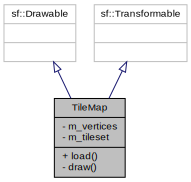
\includegraphics[width=264pt]{classTileMap__inherit__graph}
\end{center}
\end{figure}


Collaboration diagram for Tile\+Map\+:
\nopagebreak
\begin{figure}[H]
\begin{center}
\leavevmode
\includegraphics[width=264pt]{classTileMap__coll__graph}
\end{center}
\end{figure}
\subsection*{Public Member Functions}
\begin{DoxyCompactItemize}
\item 
bool \hyperlink{classTileMap_a5bc3325e2382599c3f986ac64481e832}{load} (const std\+::string \&tileset, sf\+::\+Vector2u tile\+Size, const int $\ast$tiles, unsigned int width, unsigned int height)
\end{DoxyCompactItemize}
\subsection*{Private Member Functions}
\begin{DoxyCompactItemize}
\item 
virtual void \hyperlink{classTileMap_a52562e9fb37f32fc482d7d64a2e48630}{draw} (sf\+::\+Render\+Target \&target, sf\+::\+Render\+States states) const
\end{DoxyCompactItemize}
\subsection*{Private Attributes}
\begin{DoxyCompactItemize}
\item 
sf\+::\+Vertex\+Array \hyperlink{classTileMap_a1070824d191a06562a31df73cbe7fe99}{m\+\_\+vertices}
\item 
sf\+::\+Texture \hyperlink{classTileMap_a8be6cb9e600cfd213ba6499aabbcc50b}{m\+\_\+tileset}
\end{DoxyCompactItemize}


\subsection{Member Function Documentation}
\mbox{\Hypertarget{classTileMap_a52562e9fb37f32fc482d7d64a2e48630}\label{classTileMap_a52562e9fb37f32fc482d7d64a2e48630}} 
\index{Tile\+Map@{Tile\+Map}!draw@{draw}}
\index{draw@{draw}!Tile\+Map@{Tile\+Map}}
\subsubsection{\texorpdfstring{draw()}{draw()}}
{\footnotesize\ttfamily virtual void Tile\+Map\+::draw (\begin{DoxyParamCaption}\item[{sf\+::\+Render\+Target \&}]{target,  }\item[{sf\+::\+Render\+States}]{states }\end{DoxyParamCaption}) const\hspace{0.3cm}{\ttfamily [inline]}, {\ttfamily [private]}, {\ttfamily [virtual]}}

\mbox{\Hypertarget{classTileMap_a5bc3325e2382599c3f986ac64481e832}\label{classTileMap_a5bc3325e2382599c3f986ac64481e832}} 
\index{Tile\+Map@{Tile\+Map}!load@{load}}
\index{load@{load}!Tile\+Map@{Tile\+Map}}
\subsubsection{\texorpdfstring{load()}{load()}}
{\footnotesize\ttfamily bool Tile\+Map\+::load (\begin{DoxyParamCaption}\item[{const std\+::string \&}]{tileset,  }\item[{sf\+::\+Vector2u}]{tile\+Size,  }\item[{const int $\ast$}]{tiles,  }\item[{unsigned int}]{width,  }\item[{unsigned int}]{height }\end{DoxyParamCaption})\hspace{0.3cm}{\ttfamily [inline]}}



\subsection{Member Data Documentation}
\mbox{\Hypertarget{classTileMap_a8be6cb9e600cfd213ba6499aabbcc50b}\label{classTileMap_a8be6cb9e600cfd213ba6499aabbcc50b}} 
\index{Tile\+Map@{Tile\+Map}!m\+\_\+tileset@{m\+\_\+tileset}}
\index{m\+\_\+tileset@{m\+\_\+tileset}!Tile\+Map@{Tile\+Map}}
\subsubsection{\texorpdfstring{m\+\_\+tileset}{m\_tileset}}
{\footnotesize\ttfamily sf\+::\+Texture Tile\+Map\+::m\+\_\+tileset\hspace{0.3cm}{\ttfamily [private]}}

\mbox{\Hypertarget{classTileMap_a1070824d191a06562a31df73cbe7fe99}\label{classTileMap_a1070824d191a06562a31df73cbe7fe99}} 
\index{Tile\+Map@{Tile\+Map}!m\+\_\+vertices@{m\+\_\+vertices}}
\index{m\+\_\+vertices@{m\+\_\+vertices}!Tile\+Map@{Tile\+Map}}
\subsubsection{\texorpdfstring{m\+\_\+vertices}{m\_vertices}}
{\footnotesize\ttfamily sf\+::\+Vertex\+Array Tile\+Map\+::m\+\_\+vertices\hspace{0.3cm}{\ttfamily [private]}}



The documentation for this class was generated from the following file\+:\begin{DoxyCompactItemize}
\item 
/mnt/hdd/\+C0de/\+Engines/\+S\+F\+M\+L/\+S\+F\+M\+L\+\_\+\+Engine/include/\hyperlink{TileMap_8hpp}{Tile\+Map.\+hpp}\end{DoxyCompactItemize}

\chapter{File Documentation}
\hypertarget{AssetManager_8hpp}{}\section{/mnt/hdd/\+C0de/\+Engines/\+S\+F\+M\+L/\+S\+F\+M\+L\+\_\+\+Engine/include/\+Asset\+Manager.hpp File Reference}
\label{AssetManager_8hpp}\index{/mnt/hdd/\+C0de/\+Engines/\+S\+F\+M\+L/\+S\+F\+M\+L\+\_\+\+Engine/include/\+Asset\+Manager.\+hpp@{/mnt/hdd/\+C0de/\+Engines/\+S\+F\+M\+L/\+S\+F\+M\+L\+\_\+\+Engine/include/\+Asset\+Manager.\+hpp}}
{\ttfamily \#include $<$map$>$}\newline
{\ttfamily \#include $<$S\+F\+M\+L/\+Graphics.\+hpp$>$}\newline
Include dependency graph for Asset\+Manager.\+hpp\+:
\nopagebreak
\begin{figure}[H]
\begin{center}
\leavevmode
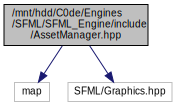
\includegraphics[width=248pt]{AssetManager_8hpp__incl}
\end{center}
\end{figure}
This graph shows which files directly or indirectly include this file\+:
\nopagebreak
\begin{figure}[H]
\begin{center}
\leavevmode
\includegraphics[width=350pt]{AssetManager_8hpp__dep__incl}
\end{center}
\end{figure}
\subsection*{Classes}
\begin{DoxyCompactItemize}
\item 
class \hyperlink{classSekander_1_1AssetManager}{Sekander\+::\+Asset\+Manager}
\end{DoxyCompactItemize}
\subsection*{Namespaces}
\begin{DoxyCompactItemize}
\item 
 \hyperlink{namespaceSekander}{Sekander}
\end{DoxyCompactItemize}

\hypertarget{Bullet_8hpp}{}\section{/mnt/hdd/\+C0de/\+Engines/\+S\+F\+M\+L/\+S\+F\+M\+L\+\_\+\+Engine/include/\+Bullet.hpp File Reference}
\label{Bullet_8hpp}\index{/mnt/hdd/\+C0de/\+Engines/\+S\+F\+M\+L/\+S\+F\+M\+L\+\_\+\+Engine/include/\+Bullet.\+hpp@{/mnt/hdd/\+C0de/\+Engines/\+S\+F\+M\+L/\+S\+F\+M\+L\+\_\+\+Engine/include/\+Bullet.\+hpp}}
{\ttfamily \#include \char`\"{}Game\+World.\+hpp\char`\"{}}\newline
{\ttfamily \#include $<$iostream$>$}\newline
Include dependency graph for Bullet.\+hpp\+:
\nopagebreak
\begin{figure}[H]
\begin{center}
\leavevmode
\includegraphics[width=350pt]{Bullet_8hpp__incl}
\end{center}
\end{figure}
This graph shows which files directly or indirectly include this file\+:
\nopagebreak
\begin{figure}[H]
\begin{center}
\leavevmode
\includegraphics[width=350pt]{Bullet_8hpp__dep__incl}
\end{center}
\end{figure}
\subsection*{Classes}
\begin{DoxyCompactItemize}
\item 
class \hyperlink{classSekander_1_1Bullet}{Sekander\+::\+Bullet}
\end{DoxyCompactItemize}
\subsection*{Namespaces}
\begin{DoxyCompactItemize}
\item 
 \hyperlink{namespaceSekander}{Sekander}
\end{DoxyCompactItemize}

\hypertarget{Button_8hpp}{}\section{/mnt/hdd/\+C0de/\+Engines/\+S\+F\+M\+L/\+S\+F\+M\+L\+\_\+\+Engine/include/\+Button.hpp File Reference}
\label{Button_8hpp}\index{/mnt/hdd/\+C0de/\+Engines/\+S\+F\+M\+L/\+S\+F\+M\+L\+\_\+\+Engine/include/\+Button.\+hpp@{/mnt/hdd/\+C0de/\+Engines/\+S\+F\+M\+L/\+S\+F\+M\+L\+\_\+\+Engine/include/\+Button.\+hpp}}
{\ttfamily \#include $<$S\+F\+M\+L/\+Graphics.\+hpp$>$}\newline
{\ttfamily \#include \char`\"{}Game.\+hpp\char`\"{}}\newline
Include dependency graph for Button.\+hpp\+:
\nopagebreak
\begin{figure}[H]
\begin{center}
\leavevmode
\includegraphics[width=350pt]{Button_8hpp__incl}
\end{center}
\end{figure}
\subsection*{Classes}
\begin{DoxyCompactItemize}
\item 
class \hyperlink{classSekander_1_1Button}{Sekander\+::\+Button}
\end{DoxyCompactItemize}
\subsection*{Namespaces}
\begin{DoxyCompactItemize}
\item 
 \hyperlink{namespaceSekander}{Sekander}
\end{DoxyCompactItemize}

\hypertarget{DEFINITIONS_8hpp}{}\section{/mnt/hdd/\+C0de/\+Engines/\+S\+F\+M\+L/\+S\+F\+M\+L\+\_\+\+Engine/include/\+D\+E\+F\+I\+N\+I\+T\+I\+O\+NS.hpp File Reference}
\label{DEFINITIONS_8hpp}\index{/mnt/hdd/\+C0de/\+Engines/\+S\+F\+M\+L/\+S\+F\+M\+L\+\_\+\+Engine/include/\+D\+E\+F\+I\+N\+I\+T\+I\+O\+N\+S.\+hpp@{/mnt/hdd/\+C0de/\+Engines/\+S\+F\+M\+L/\+S\+F\+M\+L\+\_\+\+Engine/include/\+D\+E\+F\+I\+N\+I\+T\+I\+O\+N\+S.\+hpp}}
This graph shows which files directly or indirectly include this file\+:
\nopagebreak
\begin{figure}[H]
\begin{center}
\leavevmode
\includegraphics[width=350pt]{DEFINITIONS_8hpp__dep__incl}
\end{center}
\end{figure}
\subsection*{Macros}
\begin{DoxyCompactItemize}
\item 
\#define \hyperlink{DEFINITIONS_8hpp_a2cd109632a6dcccaa80b43561b1ab700}{S\+C\+R\+E\+E\+N\+\_\+\+W\+I\+D\+TH}~1366
\item 
\#define \hyperlink{DEFINITIONS_8hpp_a6974d08a74da681b3957b2fead2608b8}{S\+C\+R\+E\+E\+N\+\_\+\+H\+E\+I\+G\+HT}~768
\item 
\#define \hyperlink{DEFINITIONS_8hpp_a06d8261983af6a29c9587c55cf2481d4}{S\+P\+L\+A\+S\+H\+\_\+\+S\+T\+A\+T\+E\+\_\+\+S\+H\+O\+W\+\_\+\+T\+I\+ME}~7.\+0
\item 
\#define \hyperlink{DEFINITIONS_8hpp_a14e8e00fb25eb45538692a5455119938}{S\+P\+L\+A\+S\+H\+\_\+\+S\+C\+E\+N\+E\+\_\+\+B\+A\+C\+K\+G\+R\+O\+U\+N\+D\+\_\+\+F\+I\+L\+E\+P\+A\+TH}~\char`\"{}Resources/res/nintendo-\/switch-\/minimal.\+jpg\char`\"{}
\item 
\#define \hyperlink{DEFINITIONS_8hpp_a04cda72602d3ae59216d8aff93ea9b6a}{M\+A\+I\+N\+\_\+\+M\+E\+N\+U\+\_\+\+B\+A\+C\+K\+G\+R\+O\+U\+N\+D\+\_\+\+F\+I\+L\+E\+P\+A\+TH}~\char`\"{}Resources/res/main\+\_\+menu.\+png\char`\"{}
\item 
\#define \hyperlink{DEFINITIONS_8hpp_a1811efff299e4d80a481decf69ded942}{G\+A\+M\+E\+\_\+\+B\+A\+C\+K\+G\+R\+O\+U\+N\+D\+\_\+\+F\+I\+L\+E\+P\+A\+TH}~\char`\"{}Resources/res/blue\+\_\+background.\+jpg\char`\"{}
\item 
\#define \hyperlink{DEFINITIONS_8hpp_a3d379e9e10cc6055a70e14d69e1a6c43}{G\+A\+M\+E\+\_\+\+O\+V\+E\+R\+\_\+\+B\+A\+C\+K\+G\+R\+O\+U\+N\+D\+\_\+\+F\+I\+L\+E\+P\+A\+TH}~\char`\"{}Resources/res/game\+\_\+over\+\_\+background.\+jpg\char`\"{}
\item 
\#define \hyperlink{DEFINITIONS_8hpp_a3f1861b2f2234d76b769a649afe4e434}{G\+A\+M\+E\+\_\+\+T\+I\+T\+L\+E\+\_\+\+F\+I\+L\+E\+P\+A\+TH}~\char`\"{}Resources/res/alexi.\+png\char`\"{}
\item 
\#define \hyperlink{DEFINITIONS_8hpp_ae522dd0ecdf21fe585e5b033e78b019f}{P\+L\+A\+Y\+\_\+\+B\+U\+T\+T\+O\+N\+\_\+\+F\+I\+L\+E\+P\+A\+TH}~\char`\"{}Resources/res/play\+\_\+bt.\+png\char`\"{}
\item 
\#define \hyperlink{DEFINITIONS_8hpp_a6b473f341c95c363b0eb421ce153414f}{P\+I\+P\+E\+\_\+\+U\+P\+\_\+\+F\+I\+L\+E\+P\+A\+TH}~\char`\"{}Resources/res/Pipe\+Up.\+png\char`\"{}
\item 
\#define \hyperlink{DEFINITIONS_8hpp_aeb5574e86ebb961f809fb421580d4cd3}{P\+I\+P\+E\+\_\+\+D\+O\+W\+N\+\_\+\+F\+I\+L\+E\+P\+A\+TH}~\char`\"{}Resources/res/Pipe\+Down.\+png\char`\"{}
\item 
\#define \hyperlink{DEFINITIONS_8hpp_ad4c6bcb54d444dfa2e1956afd21f6cba}{P\+I\+P\+E\+\_\+\+S\+C\+O\+R\+I\+N\+G\+\_\+\+F\+I\+L\+E\+P\+A\+TH}~\char`\"{}Resources/res/Invisible\+Scoring\+Pipe.\+png\char`\"{}
\item 
\#define \hyperlink{DEFINITIONS_8hpp_a6af39d3bc891a2319bef3927d6bd5091}{H\+I\+G\+H\+\_\+\+S\+C\+O\+R\+E\+\_\+\+F\+I\+L\+E\+P\+A\+TH}~\char`\"{}Resources/High\+Score.\+txt\char`\"{}
\item 
\#define \hyperlink{DEFINITIONS_8hpp_a726c2d9f0f49eb3ac24bcd5bea667d9c}{L\+A\+N\+D\+\_\+\+F\+I\+L\+E\+P\+A\+TH}~\char`\"{}Resources/res/land.\+png\char`\"{}
\item 
\#define \hyperlink{DEFINITIONS_8hpp_a8e19282a32afb23d837abe54f69e7511}{P\+I\+P\+E\+\_\+\+M\+O\+V\+E\+M\+E\+N\+T\+\_\+\+S\+P\+P\+ED}~200.\+0f
\item 
\#define \hyperlink{DEFINITIONS_8hpp_a52dd4b47013f7da150546d76c2f8d159}{P\+I\+P\+E\+\_\+\+S\+P\+A\+W\+N\+\_\+\+F\+R\+E\+Q\+U\+E\+N\+CY}~3.\+0f;
\item 
\#define \hyperlink{DEFINITIONS_8hpp_afd42bce708882551989569c0601727d4}{B\+I\+R\+D\+\_\+\+F\+R\+A\+M\+E\+\_\+1\+\_\+\+F\+I\+I\+L\+E\+P\+A\+TH}~\char`\"{}Resources/res/bird-\/01.png\char`\"{}
\item 
\#define \hyperlink{DEFINITIONS_8hpp_ae790870144221367765c28196da08405}{B\+I\+R\+D\+\_\+\+F\+R\+A\+M\+E\+\_\+2\+\_\+\+F\+I\+I\+L\+E\+P\+A\+TH}~\char`\"{}Resources/res/bird-\/02.png\char`\"{}
\item 
\#define \hyperlink{DEFINITIONS_8hpp_abba75c936a4444d7915cc9f8ae208e6a}{B\+I\+R\+D\+\_\+\+F\+R\+A\+M\+E\+\_\+3\+\_\+\+F\+I\+I\+L\+E\+P\+A\+TH}~\char`\"{}Resources/res/bird-\/03.png\char`\"{}
\item 
\#define \hyperlink{DEFINITIONS_8hpp_a5fc7ac6aac5a5302a7722346dd7243e7}{B\+I\+R\+D\+\_\+\+F\+R\+A\+M\+E\+\_\+4\+\_\+\+F\+I\+I\+L\+E\+P\+A\+TH}~\char`\"{}Resources/res/bird-\/04.png\char`\"{}
\item 
\#define \hyperlink{DEFINITIONS_8hpp_ab3dfd2a14893371759479ac6ac57b159}{P\+L\+A\+Y\+E\+R\+\_\+\+F\+I\+L\+E\+P\+A\+TH}~\char`\"{}Resources/res/sprite\+\_\+sheet.\+png\char`\"{}
\item 
\#define \hyperlink{DEFINITIONS_8hpp_aa8ed31a587192401b0614d619133ca6b}{M\+A\+G\+I\+K\+\_\+\+F\+I\+L\+E\+P\+A\+TH}~\char`\"{}Resources/res/magik8.\+png\char`\"{}
\item 
\#define \hyperlink{DEFINITIONS_8hpp_a70d3ca2da5f22b976b64e44a84efb7d9}{F\+O\+N\+T\+\_\+\+F\+I\+L\+E\+P\+A\+TH}~\char`\"{}Resources/fonts/Flappy\+Font.\+ttf\char`\"{}
\item 
\#define \hyperlink{DEFINITIONS_8hpp_ab406f792732179484ea303087b5e09b0}{G\+A\+M\+E\+\_\+\+O\+V\+E\+R\+\_\+\+T\+I\+T\+L\+E\+\_\+\+F\+I\+L\+E\+P\+A\+TH}~\char`\"{}Resources/res/Game-\/Over-\/Title.\+png\char`\"{}
\item 
\#define \hyperlink{DEFINITIONS_8hpp_a18f503e0e4436135f86f7c3a1f49acb9}{G\+A\+M\+E\+\_\+\+O\+V\+E\+R\+\_\+\+B\+O\+D\+Y\+\_\+\+F\+I\+L\+E\+P\+A\+TH}~\char`\"{}Resources/res/Game-\/Over-\/Body.\+png\char`\"{}
\item 
\#define \hyperlink{DEFINITIONS_8hpp_ae4dd059e801b991d488e234492874af9}{H\+I\+T\+\_\+\+S\+O\+U\+N\+D\+\_\+\+F\+I\+L\+E\+P\+A\+TH}~\char`\"{}Resources/audio/Hit.\+wav\char`\"{}
\item 
\#define \hyperlink{DEFINITIONS_8hpp_a6396cc6dcf0b43f595061ccc6d0a3fc8}{P\+O\+I\+N\+T\+\_\+\+S\+O\+U\+N\+D\+\_\+\+F\+I\+L\+E\+P\+A\+TH}~\char`\"{}Resources/audio/Point.\+wav\char`\"{}
\item 
\#define \hyperlink{DEFINITIONS_8hpp_a66fd1f4a51ae74fffc582a2b945ef0a5}{W\+I\+N\+G\+\_\+\+S\+O\+U\+N\+D\+\_\+\+F\+I\+L\+E\+P\+A\+TH}~\char`\"{}Resources/audio/Wing.\+wav\char`\"{}
\item 
\#define \hyperlink{DEFINITIONS_8hpp_a568d4bb6a0e4a40768c11ab561f607eb}{B\+I\+R\+D\+\_\+\+A\+N\+I\+M\+A\+T\+I\+O\+N\+\_\+\+D\+U\+R\+A\+T\+I\+ON}~0.\+5f
\item 
\#define \hyperlink{DEFINITIONS_8hpp_a0bb93e4bcc4fa20ae7420e2e431eaa31}{B\+I\+R\+D\+\_\+\+S\+T\+A\+T\+E\+\_\+\+S\+T\+I\+LL}~1
\item 
\#define \hyperlink{DEFINITIONS_8hpp_aeab9a0470159735954c0ba878d614746}{B\+I\+R\+D\+\_\+\+S\+T\+A\+T\+E\+\_\+\+F\+A\+L\+L\+I\+NG}~2
\item 
\#define \hyperlink{DEFINITIONS_8hpp_ad06cf05af0fa05c51ff78ac4b853293e}{B\+I\+R\+D\+\_\+\+S\+T\+A\+T\+E\+\_\+\+F\+L\+Y\+I\+NG}~3
\item 
\#define \hyperlink{DEFINITIONS_8hpp_a6801baa546c6112d19eb095111d24720}{G\+R\+A\+V\+I\+TY}~350.\+0f
\item 
\#define \hyperlink{DEFINITIONS_8hpp_ad21551cb06a035460f5c8f64d833cee2}{F\+L\+Y\+I\+N\+G\+\_\+\+S\+P\+E\+ED}~350.\+0f
\item 
\#define \hyperlink{DEFINITIONS_8hpp_a614aa38aee17fa248602bb4839f4821d}{F\+L\+Y\+I\+N\+G\+\_\+\+D\+U\+R\+A\+T\+I\+ON}~0.\+25f
\item 
\#define \hyperlink{DEFINITIONS_8hpp_a36867b302379cb0e4d90f9eff433212c}{S\+P\+R\+I\+T\+E\+\_\+\+W\+I\+D\+TH}~32
\item 
\#define \hyperlink{DEFINITIONS_8hpp_a76f347c245a262bf164389951c1d185e}{S\+P\+R\+I\+T\+E\+\_\+\+H\+E\+I\+G\+HT}~32
\item 
\#define \hyperlink{DEFINITIONS_8hpp_aa5845ccf3e16393ac0731a5d5a46a359}{D\+I\+R\+E\+C\+T\+I\+O\+N\+\_\+\+Y\+\_\+\+D\+O\+W\+N\+\_\+\+I\+N\+I\+T\+AL}~0
\item 
\#define \hyperlink{DEFINITIONS_8hpp_af2dde0469b6f8f67be28d4ff1af37a32}{D\+I\+R\+E\+T\+I\+O\+N\+\_\+\+Y\+\_\+\+L\+E\+F\+T\+\_\+\+I\+N\+I\+T\+AL}~1
\item 
\#define \hyperlink{DEFINITIONS_8hpp_a680549b56d8e550f167cbf4f49381324}{D\+I\+R\+E\+C\+T\+I\+O\+N\+\_\+\+Y\+\_\+\+R\+I\+G\+H\+T\+\_\+\+I\+N\+I\+T\+AL}~2
\item 
\#define \hyperlink{DEFINITIONS_8hpp_ae39044b3eaa6771cb4f851ab28334bee}{D\+I\+R\+E\+C\+T\+I\+O\+N\+\_\+\+Y\+\_\+\+U\+P\+\_\+\+I\+N\+I\+T\+AL}~3
\item 
\#define \hyperlink{DEFINITIONS_8hpp_af5619059410adc9da27da47d48bc0208}{D\+I\+R\+E\+C\+T\+I\+O\+N\+\_\+\+X\+\_\+\+D\+O\+W\+N\+\_\+\+I\+N\+I\+T\+AL}~0
\item 
\#define \hyperlink{DEFINITIONS_8hpp_acd0fa0d6189393268560cdbe0977a20b}{D\+I\+R\+E\+C\+T\+I\+O\+N\+\_\+\+X\+\_\+\+L\+E\+F\+T\+\_\+\+I\+N\+I\+T\+AL}~0
\item 
\#define \hyperlink{DEFINITIONS_8hpp_a5df2817928b9d616365d41716225855b}{D\+I\+R\+E\+C\+T\+I\+O\+N\+\_\+\+X\+\_\+\+R\+I\+G\+H\+T\+\_\+\+I\+N\+I\+T\+AL}~0
\item 
\#define \hyperlink{DEFINITIONS_8hpp_a1654dbfe1ea5b669d521f299b32dcbb4}{D\+I\+R\+E\+C\+T\+I\+O\+N\+\_\+\+X\+\_\+\+U\+P\+\_\+\+I\+N\+I\+T\+AL}~0
\item 
\#define \hyperlink{DEFINITIONS_8hpp_a59c1849a23db0716bc2c2de300c35f1a}{X\+\_\+\+F\+R\+A\+M\+E\+S\+\_\+1}~0
\item 
\#define \hyperlink{DEFINITIONS_8hpp_a47eae7a523c04d9836507102716e0281}{X\+\_\+\+F\+R\+A\+M\+E\+S\+\_\+2}~1
\item 
\#define \hyperlink{DEFINITIONS_8hpp_af9bdb6427c8fdc0a878037fcb2e163b5}{X\+\_\+\+F\+R\+A\+M\+E\+S\+\_\+3}~2
\item 
\#define \hyperlink{DEFINITIONS_8hpp_abbfb1b8e88373781c6238d647110f5d2}{D\+E\+G\+T\+O\+R\+AD}~0.\+0174532925199432957f
\item 
\#define \hyperlink{DEFINITIONS_8hpp_a9fcbc53371e9a60b983c6b338537aa40}{R\+A\+D\+T\+O\+D\+EG}~57.\+295779513082320876f
\item 
\#define \hyperlink{DEFINITIONS_8hpp_ab3c0e39118375eb14be39f35057eb94c}{F\+L\+A\+S\+H\+\_\+\+S\+P\+E\+ED}~1500.\+0f
\item 
\#define \hyperlink{DEFINITIONS_8hpp_a0b73c5aa67be999a8922f4ddfce6e4a9}{T\+I\+M\+E\+\_\+\+B\+E\+F\+O\+R\+E\+\_\+\+G\+A\+M\+E\+\_\+\+O\+V\+E\+R\+\_\+\+A\+P\+P\+E\+A\+RS}~1.\+5f
\end{DoxyCompactItemize}
\subsection*{Enumerations}
\begin{DoxyCompactItemize}
\item 
enum \hyperlink{DEFINITIONS_8hpp_a680d333abdfd9a5053a12072f8364fe4}{Game\+\_\+\+States} \{ \hyperlink{DEFINITIONS_8hpp_a680d333abdfd9a5053a12072f8364fe4a79e0fbea0598e65a4789cdf35b8d7c52}{e\+\_\+\+Ready}, 
\hyperlink{DEFINITIONS_8hpp_a680d333abdfd9a5053a12072f8364fe4ad1ce8495b35f97ab21085a7c0779376a}{e\+\_\+\+Playing}, 
\hyperlink{DEFINITIONS_8hpp_a680d333abdfd9a5053a12072f8364fe4acd81b021f4bf6b2c062809783e227b59}{e\+\_\+\+Game\+Over}
 \}
\end{DoxyCompactItemize}


\subsection{Macro Definition Documentation}
\mbox{\Hypertarget{DEFINITIONS_8hpp_a568d4bb6a0e4a40768c11ab561f607eb}\label{DEFINITIONS_8hpp_a568d4bb6a0e4a40768c11ab561f607eb}} 
\index{D\+E\+F\+I\+N\+I\+T\+I\+O\+N\+S.\+hpp@{D\+E\+F\+I\+N\+I\+T\+I\+O\+N\+S.\+hpp}!B\+I\+R\+D\+\_\+\+A\+N\+I\+M\+A\+T\+I\+O\+N\+\_\+\+D\+U\+R\+A\+T\+I\+ON@{B\+I\+R\+D\+\_\+\+A\+N\+I\+M\+A\+T\+I\+O\+N\+\_\+\+D\+U\+R\+A\+T\+I\+ON}}
\index{B\+I\+R\+D\+\_\+\+A\+N\+I\+M\+A\+T\+I\+O\+N\+\_\+\+D\+U\+R\+A\+T\+I\+ON@{B\+I\+R\+D\+\_\+\+A\+N\+I\+M\+A\+T\+I\+O\+N\+\_\+\+D\+U\+R\+A\+T\+I\+ON}!D\+E\+F\+I\+N\+I\+T\+I\+O\+N\+S.\+hpp@{D\+E\+F\+I\+N\+I\+T\+I\+O\+N\+S.\+hpp}}
\subsubsection{\texorpdfstring{B\+I\+R\+D\+\_\+\+A\+N\+I\+M\+A\+T\+I\+O\+N\+\_\+\+D\+U\+R\+A\+T\+I\+ON}{BIRD\_ANIMATION\_DURATION}}
{\footnotesize\ttfamily \#define B\+I\+R\+D\+\_\+\+A\+N\+I\+M\+A\+T\+I\+O\+N\+\_\+\+D\+U\+R\+A\+T\+I\+ON~0.\+5f}

\mbox{\Hypertarget{DEFINITIONS_8hpp_afd42bce708882551989569c0601727d4}\label{DEFINITIONS_8hpp_afd42bce708882551989569c0601727d4}} 
\index{D\+E\+F\+I\+N\+I\+T\+I\+O\+N\+S.\+hpp@{D\+E\+F\+I\+N\+I\+T\+I\+O\+N\+S.\+hpp}!B\+I\+R\+D\+\_\+\+F\+R\+A\+M\+E\+\_\+1\+\_\+\+F\+I\+I\+L\+E\+P\+A\+TH@{B\+I\+R\+D\+\_\+\+F\+R\+A\+M\+E\+\_\+1\+\_\+\+F\+I\+I\+L\+E\+P\+A\+TH}}
\index{B\+I\+R\+D\+\_\+\+F\+R\+A\+M\+E\+\_\+1\+\_\+\+F\+I\+I\+L\+E\+P\+A\+TH@{B\+I\+R\+D\+\_\+\+F\+R\+A\+M\+E\+\_\+1\+\_\+\+F\+I\+I\+L\+E\+P\+A\+TH}!D\+E\+F\+I\+N\+I\+T\+I\+O\+N\+S.\+hpp@{D\+E\+F\+I\+N\+I\+T\+I\+O\+N\+S.\+hpp}}
\subsubsection{\texorpdfstring{B\+I\+R\+D\+\_\+\+F\+R\+A\+M\+E\+\_\+1\+\_\+\+F\+I\+I\+L\+E\+P\+A\+TH}{BIRD\_FRAME\_1\_FIILEPATH}}
{\footnotesize\ttfamily \#define B\+I\+R\+D\+\_\+\+F\+R\+A\+M\+E\+\_\+1\+\_\+\+F\+I\+I\+L\+E\+P\+A\+TH~\char`\"{}Resources/res/bird-\/01.png\char`\"{}}

\mbox{\Hypertarget{DEFINITIONS_8hpp_ae790870144221367765c28196da08405}\label{DEFINITIONS_8hpp_ae790870144221367765c28196da08405}} 
\index{D\+E\+F\+I\+N\+I\+T\+I\+O\+N\+S.\+hpp@{D\+E\+F\+I\+N\+I\+T\+I\+O\+N\+S.\+hpp}!B\+I\+R\+D\+\_\+\+F\+R\+A\+M\+E\+\_\+2\+\_\+\+F\+I\+I\+L\+E\+P\+A\+TH@{B\+I\+R\+D\+\_\+\+F\+R\+A\+M\+E\+\_\+2\+\_\+\+F\+I\+I\+L\+E\+P\+A\+TH}}
\index{B\+I\+R\+D\+\_\+\+F\+R\+A\+M\+E\+\_\+2\+\_\+\+F\+I\+I\+L\+E\+P\+A\+TH@{B\+I\+R\+D\+\_\+\+F\+R\+A\+M\+E\+\_\+2\+\_\+\+F\+I\+I\+L\+E\+P\+A\+TH}!D\+E\+F\+I\+N\+I\+T\+I\+O\+N\+S.\+hpp@{D\+E\+F\+I\+N\+I\+T\+I\+O\+N\+S.\+hpp}}
\subsubsection{\texorpdfstring{B\+I\+R\+D\+\_\+\+F\+R\+A\+M\+E\+\_\+2\+\_\+\+F\+I\+I\+L\+E\+P\+A\+TH}{BIRD\_FRAME\_2\_FIILEPATH}}
{\footnotesize\ttfamily \#define B\+I\+R\+D\+\_\+\+F\+R\+A\+M\+E\+\_\+2\+\_\+\+F\+I\+I\+L\+E\+P\+A\+TH~\char`\"{}Resources/res/bird-\/02.png\char`\"{}}

\mbox{\Hypertarget{DEFINITIONS_8hpp_abba75c936a4444d7915cc9f8ae208e6a}\label{DEFINITIONS_8hpp_abba75c936a4444d7915cc9f8ae208e6a}} 
\index{D\+E\+F\+I\+N\+I\+T\+I\+O\+N\+S.\+hpp@{D\+E\+F\+I\+N\+I\+T\+I\+O\+N\+S.\+hpp}!B\+I\+R\+D\+\_\+\+F\+R\+A\+M\+E\+\_\+3\+\_\+\+F\+I\+I\+L\+E\+P\+A\+TH@{B\+I\+R\+D\+\_\+\+F\+R\+A\+M\+E\+\_\+3\+\_\+\+F\+I\+I\+L\+E\+P\+A\+TH}}
\index{B\+I\+R\+D\+\_\+\+F\+R\+A\+M\+E\+\_\+3\+\_\+\+F\+I\+I\+L\+E\+P\+A\+TH@{B\+I\+R\+D\+\_\+\+F\+R\+A\+M\+E\+\_\+3\+\_\+\+F\+I\+I\+L\+E\+P\+A\+TH}!D\+E\+F\+I\+N\+I\+T\+I\+O\+N\+S.\+hpp@{D\+E\+F\+I\+N\+I\+T\+I\+O\+N\+S.\+hpp}}
\subsubsection{\texorpdfstring{B\+I\+R\+D\+\_\+\+F\+R\+A\+M\+E\+\_\+3\+\_\+\+F\+I\+I\+L\+E\+P\+A\+TH}{BIRD\_FRAME\_3\_FIILEPATH}}
{\footnotesize\ttfamily \#define B\+I\+R\+D\+\_\+\+F\+R\+A\+M\+E\+\_\+3\+\_\+\+F\+I\+I\+L\+E\+P\+A\+TH~\char`\"{}Resources/res/bird-\/03.png\char`\"{}}

\mbox{\Hypertarget{DEFINITIONS_8hpp_a5fc7ac6aac5a5302a7722346dd7243e7}\label{DEFINITIONS_8hpp_a5fc7ac6aac5a5302a7722346dd7243e7}} 
\index{D\+E\+F\+I\+N\+I\+T\+I\+O\+N\+S.\+hpp@{D\+E\+F\+I\+N\+I\+T\+I\+O\+N\+S.\+hpp}!B\+I\+R\+D\+\_\+\+F\+R\+A\+M\+E\+\_\+4\+\_\+\+F\+I\+I\+L\+E\+P\+A\+TH@{B\+I\+R\+D\+\_\+\+F\+R\+A\+M\+E\+\_\+4\+\_\+\+F\+I\+I\+L\+E\+P\+A\+TH}}
\index{B\+I\+R\+D\+\_\+\+F\+R\+A\+M\+E\+\_\+4\+\_\+\+F\+I\+I\+L\+E\+P\+A\+TH@{B\+I\+R\+D\+\_\+\+F\+R\+A\+M\+E\+\_\+4\+\_\+\+F\+I\+I\+L\+E\+P\+A\+TH}!D\+E\+F\+I\+N\+I\+T\+I\+O\+N\+S.\+hpp@{D\+E\+F\+I\+N\+I\+T\+I\+O\+N\+S.\+hpp}}
\subsubsection{\texorpdfstring{B\+I\+R\+D\+\_\+\+F\+R\+A\+M\+E\+\_\+4\+\_\+\+F\+I\+I\+L\+E\+P\+A\+TH}{BIRD\_FRAME\_4\_FIILEPATH}}
{\footnotesize\ttfamily \#define B\+I\+R\+D\+\_\+\+F\+R\+A\+M\+E\+\_\+4\+\_\+\+F\+I\+I\+L\+E\+P\+A\+TH~\char`\"{}Resources/res/bird-\/04.png\char`\"{}}

\mbox{\Hypertarget{DEFINITIONS_8hpp_aeab9a0470159735954c0ba878d614746}\label{DEFINITIONS_8hpp_aeab9a0470159735954c0ba878d614746}} 
\index{D\+E\+F\+I\+N\+I\+T\+I\+O\+N\+S.\+hpp@{D\+E\+F\+I\+N\+I\+T\+I\+O\+N\+S.\+hpp}!B\+I\+R\+D\+\_\+\+S\+T\+A\+T\+E\+\_\+\+F\+A\+L\+L\+I\+NG@{B\+I\+R\+D\+\_\+\+S\+T\+A\+T\+E\+\_\+\+F\+A\+L\+L\+I\+NG}}
\index{B\+I\+R\+D\+\_\+\+S\+T\+A\+T\+E\+\_\+\+F\+A\+L\+L\+I\+NG@{B\+I\+R\+D\+\_\+\+S\+T\+A\+T\+E\+\_\+\+F\+A\+L\+L\+I\+NG}!D\+E\+F\+I\+N\+I\+T\+I\+O\+N\+S.\+hpp@{D\+E\+F\+I\+N\+I\+T\+I\+O\+N\+S.\+hpp}}
\subsubsection{\texorpdfstring{B\+I\+R\+D\+\_\+\+S\+T\+A\+T\+E\+\_\+\+F\+A\+L\+L\+I\+NG}{BIRD\_STATE\_FALLING}}
{\footnotesize\ttfamily \#define B\+I\+R\+D\+\_\+\+S\+T\+A\+T\+E\+\_\+\+F\+A\+L\+L\+I\+NG~2}

\mbox{\Hypertarget{DEFINITIONS_8hpp_ad06cf05af0fa05c51ff78ac4b853293e}\label{DEFINITIONS_8hpp_ad06cf05af0fa05c51ff78ac4b853293e}} 
\index{D\+E\+F\+I\+N\+I\+T\+I\+O\+N\+S.\+hpp@{D\+E\+F\+I\+N\+I\+T\+I\+O\+N\+S.\+hpp}!B\+I\+R\+D\+\_\+\+S\+T\+A\+T\+E\+\_\+\+F\+L\+Y\+I\+NG@{B\+I\+R\+D\+\_\+\+S\+T\+A\+T\+E\+\_\+\+F\+L\+Y\+I\+NG}}
\index{B\+I\+R\+D\+\_\+\+S\+T\+A\+T\+E\+\_\+\+F\+L\+Y\+I\+NG@{B\+I\+R\+D\+\_\+\+S\+T\+A\+T\+E\+\_\+\+F\+L\+Y\+I\+NG}!D\+E\+F\+I\+N\+I\+T\+I\+O\+N\+S.\+hpp@{D\+E\+F\+I\+N\+I\+T\+I\+O\+N\+S.\+hpp}}
\subsubsection{\texorpdfstring{B\+I\+R\+D\+\_\+\+S\+T\+A\+T\+E\+\_\+\+F\+L\+Y\+I\+NG}{BIRD\_STATE\_FLYING}}
{\footnotesize\ttfamily \#define B\+I\+R\+D\+\_\+\+S\+T\+A\+T\+E\+\_\+\+F\+L\+Y\+I\+NG~3}

\mbox{\Hypertarget{DEFINITIONS_8hpp_a0bb93e4bcc4fa20ae7420e2e431eaa31}\label{DEFINITIONS_8hpp_a0bb93e4bcc4fa20ae7420e2e431eaa31}} 
\index{D\+E\+F\+I\+N\+I\+T\+I\+O\+N\+S.\+hpp@{D\+E\+F\+I\+N\+I\+T\+I\+O\+N\+S.\+hpp}!B\+I\+R\+D\+\_\+\+S\+T\+A\+T\+E\+\_\+\+S\+T\+I\+LL@{B\+I\+R\+D\+\_\+\+S\+T\+A\+T\+E\+\_\+\+S\+T\+I\+LL}}
\index{B\+I\+R\+D\+\_\+\+S\+T\+A\+T\+E\+\_\+\+S\+T\+I\+LL@{B\+I\+R\+D\+\_\+\+S\+T\+A\+T\+E\+\_\+\+S\+T\+I\+LL}!D\+E\+F\+I\+N\+I\+T\+I\+O\+N\+S.\+hpp@{D\+E\+F\+I\+N\+I\+T\+I\+O\+N\+S.\+hpp}}
\subsubsection{\texorpdfstring{B\+I\+R\+D\+\_\+\+S\+T\+A\+T\+E\+\_\+\+S\+T\+I\+LL}{BIRD\_STATE\_STILL}}
{\footnotesize\ttfamily \#define B\+I\+R\+D\+\_\+\+S\+T\+A\+T\+E\+\_\+\+S\+T\+I\+LL~1}

\mbox{\Hypertarget{DEFINITIONS_8hpp_abbfb1b8e88373781c6238d647110f5d2}\label{DEFINITIONS_8hpp_abbfb1b8e88373781c6238d647110f5d2}} 
\index{D\+E\+F\+I\+N\+I\+T\+I\+O\+N\+S.\+hpp@{D\+E\+F\+I\+N\+I\+T\+I\+O\+N\+S.\+hpp}!D\+E\+G\+T\+O\+R\+AD@{D\+E\+G\+T\+O\+R\+AD}}
\index{D\+E\+G\+T\+O\+R\+AD@{D\+E\+G\+T\+O\+R\+AD}!D\+E\+F\+I\+N\+I\+T\+I\+O\+N\+S.\+hpp@{D\+E\+F\+I\+N\+I\+T\+I\+O\+N\+S.\+hpp}}
\subsubsection{\texorpdfstring{D\+E\+G\+T\+O\+R\+AD}{DEGTORAD}}
{\footnotesize\ttfamily \#define D\+E\+G\+T\+O\+R\+AD~0.\+0174532925199432957f}

\mbox{\Hypertarget{DEFINITIONS_8hpp_af5619059410adc9da27da47d48bc0208}\label{DEFINITIONS_8hpp_af5619059410adc9da27da47d48bc0208}} 
\index{D\+E\+F\+I\+N\+I\+T\+I\+O\+N\+S.\+hpp@{D\+E\+F\+I\+N\+I\+T\+I\+O\+N\+S.\+hpp}!D\+I\+R\+E\+C\+T\+I\+O\+N\+\_\+\+X\+\_\+\+D\+O\+W\+N\+\_\+\+I\+N\+I\+T\+AL@{D\+I\+R\+E\+C\+T\+I\+O\+N\+\_\+\+X\+\_\+\+D\+O\+W\+N\+\_\+\+I\+N\+I\+T\+AL}}
\index{D\+I\+R\+E\+C\+T\+I\+O\+N\+\_\+\+X\+\_\+\+D\+O\+W\+N\+\_\+\+I\+N\+I\+T\+AL@{D\+I\+R\+E\+C\+T\+I\+O\+N\+\_\+\+X\+\_\+\+D\+O\+W\+N\+\_\+\+I\+N\+I\+T\+AL}!D\+E\+F\+I\+N\+I\+T\+I\+O\+N\+S.\+hpp@{D\+E\+F\+I\+N\+I\+T\+I\+O\+N\+S.\+hpp}}
\subsubsection{\texorpdfstring{D\+I\+R\+E\+C\+T\+I\+O\+N\+\_\+\+X\+\_\+\+D\+O\+W\+N\+\_\+\+I\+N\+I\+T\+AL}{DIRECTION\_X\_DOWN\_INITAL}}
{\footnotesize\ttfamily \#define D\+I\+R\+E\+C\+T\+I\+O\+N\+\_\+\+X\+\_\+\+D\+O\+W\+N\+\_\+\+I\+N\+I\+T\+AL~0}

\mbox{\Hypertarget{DEFINITIONS_8hpp_acd0fa0d6189393268560cdbe0977a20b}\label{DEFINITIONS_8hpp_acd0fa0d6189393268560cdbe0977a20b}} 
\index{D\+E\+F\+I\+N\+I\+T\+I\+O\+N\+S.\+hpp@{D\+E\+F\+I\+N\+I\+T\+I\+O\+N\+S.\+hpp}!D\+I\+R\+E\+C\+T\+I\+O\+N\+\_\+\+X\+\_\+\+L\+E\+F\+T\+\_\+\+I\+N\+I\+T\+AL@{D\+I\+R\+E\+C\+T\+I\+O\+N\+\_\+\+X\+\_\+\+L\+E\+F\+T\+\_\+\+I\+N\+I\+T\+AL}}
\index{D\+I\+R\+E\+C\+T\+I\+O\+N\+\_\+\+X\+\_\+\+L\+E\+F\+T\+\_\+\+I\+N\+I\+T\+AL@{D\+I\+R\+E\+C\+T\+I\+O\+N\+\_\+\+X\+\_\+\+L\+E\+F\+T\+\_\+\+I\+N\+I\+T\+AL}!D\+E\+F\+I\+N\+I\+T\+I\+O\+N\+S.\+hpp@{D\+E\+F\+I\+N\+I\+T\+I\+O\+N\+S.\+hpp}}
\subsubsection{\texorpdfstring{D\+I\+R\+E\+C\+T\+I\+O\+N\+\_\+\+X\+\_\+\+L\+E\+F\+T\+\_\+\+I\+N\+I\+T\+AL}{DIRECTION\_X\_LEFT\_INITAL}}
{\footnotesize\ttfamily \#define D\+I\+R\+E\+C\+T\+I\+O\+N\+\_\+\+X\+\_\+\+L\+E\+F\+T\+\_\+\+I\+N\+I\+T\+AL~0}

\mbox{\Hypertarget{DEFINITIONS_8hpp_a5df2817928b9d616365d41716225855b}\label{DEFINITIONS_8hpp_a5df2817928b9d616365d41716225855b}} 
\index{D\+E\+F\+I\+N\+I\+T\+I\+O\+N\+S.\+hpp@{D\+E\+F\+I\+N\+I\+T\+I\+O\+N\+S.\+hpp}!D\+I\+R\+E\+C\+T\+I\+O\+N\+\_\+\+X\+\_\+\+R\+I\+G\+H\+T\+\_\+\+I\+N\+I\+T\+AL@{D\+I\+R\+E\+C\+T\+I\+O\+N\+\_\+\+X\+\_\+\+R\+I\+G\+H\+T\+\_\+\+I\+N\+I\+T\+AL}}
\index{D\+I\+R\+E\+C\+T\+I\+O\+N\+\_\+\+X\+\_\+\+R\+I\+G\+H\+T\+\_\+\+I\+N\+I\+T\+AL@{D\+I\+R\+E\+C\+T\+I\+O\+N\+\_\+\+X\+\_\+\+R\+I\+G\+H\+T\+\_\+\+I\+N\+I\+T\+AL}!D\+E\+F\+I\+N\+I\+T\+I\+O\+N\+S.\+hpp@{D\+E\+F\+I\+N\+I\+T\+I\+O\+N\+S.\+hpp}}
\subsubsection{\texorpdfstring{D\+I\+R\+E\+C\+T\+I\+O\+N\+\_\+\+X\+\_\+\+R\+I\+G\+H\+T\+\_\+\+I\+N\+I\+T\+AL}{DIRECTION\_X\_RIGHT\_INITAL}}
{\footnotesize\ttfamily \#define D\+I\+R\+E\+C\+T\+I\+O\+N\+\_\+\+X\+\_\+\+R\+I\+G\+H\+T\+\_\+\+I\+N\+I\+T\+AL~0}

\mbox{\Hypertarget{DEFINITIONS_8hpp_a1654dbfe1ea5b669d521f299b32dcbb4}\label{DEFINITIONS_8hpp_a1654dbfe1ea5b669d521f299b32dcbb4}} 
\index{D\+E\+F\+I\+N\+I\+T\+I\+O\+N\+S.\+hpp@{D\+E\+F\+I\+N\+I\+T\+I\+O\+N\+S.\+hpp}!D\+I\+R\+E\+C\+T\+I\+O\+N\+\_\+\+X\+\_\+\+U\+P\+\_\+\+I\+N\+I\+T\+AL@{D\+I\+R\+E\+C\+T\+I\+O\+N\+\_\+\+X\+\_\+\+U\+P\+\_\+\+I\+N\+I\+T\+AL}}
\index{D\+I\+R\+E\+C\+T\+I\+O\+N\+\_\+\+X\+\_\+\+U\+P\+\_\+\+I\+N\+I\+T\+AL@{D\+I\+R\+E\+C\+T\+I\+O\+N\+\_\+\+X\+\_\+\+U\+P\+\_\+\+I\+N\+I\+T\+AL}!D\+E\+F\+I\+N\+I\+T\+I\+O\+N\+S.\+hpp@{D\+E\+F\+I\+N\+I\+T\+I\+O\+N\+S.\+hpp}}
\subsubsection{\texorpdfstring{D\+I\+R\+E\+C\+T\+I\+O\+N\+\_\+\+X\+\_\+\+U\+P\+\_\+\+I\+N\+I\+T\+AL}{DIRECTION\_X\_UP\_INITAL}}
{\footnotesize\ttfamily \#define D\+I\+R\+E\+C\+T\+I\+O\+N\+\_\+\+X\+\_\+\+U\+P\+\_\+\+I\+N\+I\+T\+AL~0}

\mbox{\Hypertarget{DEFINITIONS_8hpp_aa5845ccf3e16393ac0731a5d5a46a359}\label{DEFINITIONS_8hpp_aa5845ccf3e16393ac0731a5d5a46a359}} 
\index{D\+E\+F\+I\+N\+I\+T\+I\+O\+N\+S.\+hpp@{D\+E\+F\+I\+N\+I\+T\+I\+O\+N\+S.\+hpp}!D\+I\+R\+E\+C\+T\+I\+O\+N\+\_\+\+Y\+\_\+\+D\+O\+W\+N\+\_\+\+I\+N\+I\+T\+AL@{D\+I\+R\+E\+C\+T\+I\+O\+N\+\_\+\+Y\+\_\+\+D\+O\+W\+N\+\_\+\+I\+N\+I\+T\+AL}}
\index{D\+I\+R\+E\+C\+T\+I\+O\+N\+\_\+\+Y\+\_\+\+D\+O\+W\+N\+\_\+\+I\+N\+I\+T\+AL@{D\+I\+R\+E\+C\+T\+I\+O\+N\+\_\+\+Y\+\_\+\+D\+O\+W\+N\+\_\+\+I\+N\+I\+T\+AL}!D\+E\+F\+I\+N\+I\+T\+I\+O\+N\+S.\+hpp@{D\+E\+F\+I\+N\+I\+T\+I\+O\+N\+S.\+hpp}}
\subsubsection{\texorpdfstring{D\+I\+R\+E\+C\+T\+I\+O\+N\+\_\+\+Y\+\_\+\+D\+O\+W\+N\+\_\+\+I\+N\+I\+T\+AL}{DIRECTION\_Y\_DOWN\_INITAL}}
{\footnotesize\ttfamily \#define D\+I\+R\+E\+C\+T\+I\+O\+N\+\_\+\+Y\+\_\+\+D\+O\+W\+N\+\_\+\+I\+N\+I\+T\+AL~0}

\mbox{\Hypertarget{DEFINITIONS_8hpp_a680549b56d8e550f167cbf4f49381324}\label{DEFINITIONS_8hpp_a680549b56d8e550f167cbf4f49381324}} 
\index{D\+E\+F\+I\+N\+I\+T\+I\+O\+N\+S.\+hpp@{D\+E\+F\+I\+N\+I\+T\+I\+O\+N\+S.\+hpp}!D\+I\+R\+E\+C\+T\+I\+O\+N\+\_\+\+Y\+\_\+\+R\+I\+G\+H\+T\+\_\+\+I\+N\+I\+T\+AL@{D\+I\+R\+E\+C\+T\+I\+O\+N\+\_\+\+Y\+\_\+\+R\+I\+G\+H\+T\+\_\+\+I\+N\+I\+T\+AL}}
\index{D\+I\+R\+E\+C\+T\+I\+O\+N\+\_\+\+Y\+\_\+\+R\+I\+G\+H\+T\+\_\+\+I\+N\+I\+T\+AL@{D\+I\+R\+E\+C\+T\+I\+O\+N\+\_\+\+Y\+\_\+\+R\+I\+G\+H\+T\+\_\+\+I\+N\+I\+T\+AL}!D\+E\+F\+I\+N\+I\+T\+I\+O\+N\+S.\+hpp@{D\+E\+F\+I\+N\+I\+T\+I\+O\+N\+S.\+hpp}}
\subsubsection{\texorpdfstring{D\+I\+R\+E\+C\+T\+I\+O\+N\+\_\+\+Y\+\_\+\+R\+I\+G\+H\+T\+\_\+\+I\+N\+I\+T\+AL}{DIRECTION\_Y\_RIGHT\_INITAL}}
{\footnotesize\ttfamily \#define D\+I\+R\+E\+C\+T\+I\+O\+N\+\_\+\+Y\+\_\+\+R\+I\+G\+H\+T\+\_\+\+I\+N\+I\+T\+AL~2}

\mbox{\Hypertarget{DEFINITIONS_8hpp_ae39044b3eaa6771cb4f851ab28334bee}\label{DEFINITIONS_8hpp_ae39044b3eaa6771cb4f851ab28334bee}} 
\index{D\+E\+F\+I\+N\+I\+T\+I\+O\+N\+S.\+hpp@{D\+E\+F\+I\+N\+I\+T\+I\+O\+N\+S.\+hpp}!D\+I\+R\+E\+C\+T\+I\+O\+N\+\_\+\+Y\+\_\+\+U\+P\+\_\+\+I\+N\+I\+T\+AL@{D\+I\+R\+E\+C\+T\+I\+O\+N\+\_\+\+Y\+\_\+\+U\+P\+\_\+\+I\+N\+I\+T\+AL}}
\index{D\+I\+R\+E\+C\+T\+I\+O\+N\+\_\+\+Y\+\_\+\+U\+P\+\_\+\+I\+N\+I\+T\+AL@{D\+I\+R\+E\+C\+T\+I\+O\+N\+\_\+\+Y\+\_\+\+U\+P\+\_\+\+I\+N\+I\+T\+AL}!D\+E\+F\+I\+N\+I\+T\+I\+O\+N\+S.\+hpp@{D\+E\+F\+I\+N\+I\+T\+I\+O\+N\+S.\+hpp}}
\subsubsection{\texorpdfstring{D\+I\+R\+E\+C\+T\+I\+O\+N\+\_\+\+Y\+\_\+\+U\+P\+\_\+\+I\+N\+I\+T\+AL}{DIRECTION\_Y\_UP\_INITAL}}
{\footnotesize\ttfamily \#define D\+I\+R\+E\+C\+T\+I\+O\+N\+\_\+\+Y\+\_\+\+U\+P\+\_\+\+I\+N\+I\+T\+AL~3}

\mbox{\Hypertarget{DEFINITIONS_8hpp_af2dde0469b6f8f67be28d4ff1af37a32}\label{DEFINITIONS_8hpp_af2dde0469b6f8f67be28d4ff1af37a32}} 
\index{D\+E\+F\+I\+N\+I\+T\+I\+O\+N\+S.\+hpp@{D\+E\+F\+I\+N\+I\+T\+I\+O\+N\+S.\+hpp}!D\+I\+R\+E\+T\+I\+O\+N\+\_\+\+Y\+\_\+\+L\+E\+F\+T\+\_\+\+I\+N\+I\+T\+AL@{D\+I\+R\+E\+T\+I\+O\+N\+\_\+\+Y\+\_\+\+L\+E\+F\+T\+\_\+\+I\+N\+I\+T\+AL}}
\index{D\+I\+R\+E\+T\+I\+O\+N\+\_\+\+Y\+\_\+\+L\+E\+F\+T\+\_\+\+I\+N\+I\+T\+AL@{D\+I\+R\+E\+T\+I\+O\+N\+\_\+\+Y\+\_\+\+L\+E\+F\+T\+\_\+\+I\+N\+I\+T\+AL}!D\+E\+F\+I\+N\+I\+T\+I\+O\+N\+S.\+hpp@{D\+E\+F\+I\+N\+I\+T\+I\+O\+N\+S.\+hpp}}
\subsubsection{\texorpdfstring{D\+I\+R\+E\+T\+I\+O\+N\+\_\+\+Y\+\_\+\+L\+E\+F\+T\+\_\+\+I\+N\+I\+T\+AL}{DIRETION\_Y\_LEFT\_INITAL}}
{\footnotesize\ttfamily \#define D\+I\+R\+E\+T\+I\+O\+N\+\_\+\+Y\+\_\+\+L\+E\+F\+T\+\_\+\+I\+N\+I\+T\+AL~1}

\mbox{\Hypertarget{DEFINITIONS_8hpp_ab3c0e39118375eb14be39f35057eb94c}\label{DEFINITIONS_8hpp_ab3c0e39118375eb14be39f35057eb94c}} 
\index{D\+E\+F\+I\+N\+I\+T\+I\+O\+N\+S.\+hpp@{D\+E\+F\+I\+N\+I\+T\+I\+O\+N\+S.\+hpp}!F\+L\+A\+S\+H\+\_\+\+S\+P\+E\+ED@{F\+L\+A\+S\+H\+\_\+\+S\+P\+E\+ED}}
\index{F\+L\+A\+S\+H\+\_\+\+S\+P\+E\+ED@{F\+L\+A\+S\+H\+\_\+\+S\+P\+E\+ED}!D\+E\+F\+I\+N\+I\+T\+I\+O\+N\+S.\+hpp@{D\+E\+F\+I\+N\+I\+T\+I\+O\+N\+S.\+hpp}}
\subsubsection{\texorpdfstring{F\+L\+A\+S\+H\+\_\+\+S\+P\+E\+ED}{FLASH\_SPEED}}
{\footnotesize\ttfamily \#define F\+L\+A\+S\+H\+\_\+\+S\+P\+E\+ED~1500.\+0f}

\mbox{\Hypertarget{DEFINITIONS_8hpp_a614aa38aee17fa248602bb4839f4821d}\label{DEFINITIONS_8hpp_a614aa38aee17fa248602bb4839f4821d}} 
\index{D\+E\+F\+I\+N\+I\+T\+I\+O\+N\+S.\+hpp@{D\+E\+F\+I\+N\+I\+T\+I\+O\+N\+S.\+hpp}!F\+L\+Y\+I\+N\+G\+\_\+\+D\+U\+R\+A\+T\+I\+ON@{F\+L\+Y\+I\+N\+G\+\_\+\+D\+U\+R\+A\+T\+I\+ON}}
\index{F\+L\+Y\+I\+N\+G\+\_\+\+D\+U\+R\+A\+T\+I\+ON@{F\+L\+Y\+I\+N\+G\+\_\+\+D\+U\+R\+A\+T\+I\+ON}!D\+E\+F\+I\+N\+I\+T\+I\+O\+N\+S.\+hpp@{D\+E\+F\+I\+N\+I\+T\+I\+O\+N\+S.\+hpp}}
\subsubsection{\texorpdfstring{F\+L\+Y\+I\+N\+G\+\_\+\+D\+U\+R\+A\+T\+I\+ON}{FLYING\_DURATION}}
{\footnotesize\ttfamily \#define F\+L\+Y\+I\+N\+G\+\_\+\+D\+U\+R\+A\+T\+I\+ON~0.\+25f}

\mbox{\Hypertarget{DEFINITIONS_8hpp_ad21551cb06a035460f5c8f64d833cee2}\label{DEFINITIONS_8hpp_ad21551cb06a035460f5c8f64d833cee2}} 
\index{D\+E\+F\+I\+N\+I\+T\+I\+O\+N\+S.\+hpp@{D\+E\+F\+I\+N\+I\+T\+I\+O\+N\+S.\+hpp}!F\+L\+Y\+I\+N\+G\+\_\+\+S\+P\+E\+ED@{F\+L\+Y\+I\+N\+G\+\_\+\+S\+P\+E\+ED}}
\index{F\+L\+Y\+I\+N\+G\+\_\+\+S\+P\+E\+ED@{F\+L\+Y\+I\+N\+G\+\_\+\+S\+P\+E\+ED}!D\+E\+F\+I\+N\+I\+T\+I\+O\+N\+S.\+hpp@{D\+E\+F\+I\+N\+I\+T\+I\+O\+N\+S.\+hpp}}
\subsubsection{\texorpdfstring{F\+L\+Y\+I\+N\+G\+\_\+\+S\+P\+E\+ED}{FLYING\_SPEED}}
{\footnotesize\ttfamily \#define F\+L\+Y\+I\+N\+G\+\_\+\+S\+P\+E\+ED~350.\+0f}

\mbox{\Hypertarget{DEFINITIONS_8hpp_a70d3ca2da5f22b976b64e44a84efb7d9}\label{DEFINITIONS_8hpp_a70d3ca2da5f22b976b64e44a84efb7d9}} 
\index{D\+E\+F\+I\+N\+I\+T\+I\+O\+N\+S.\+hpp@{D\+E\+F\+I\+N\+I\+T\+I\+O\+N\+S.\+hpp}!F\+O\+N\+T\+\_\+\+F\+I\+L\+E\+P\+A\+TH@{F\+O\+N\+T\+\_\+\+F\+I\+L\+E\+P\+A\+TH}}
\index{F\+O\+N\+T\+\_\+\+F\+I\+L\+E\+P\+A\+TH@{F\+O\+N\+T\+\_\+\+F\+I\+L\+E\+P\+A\+TH}!D\+E\+F\+I\+N\+I\+T\+I\+O\+N\+S.\+hpp@{D\+E\+F\+I\+N\+I\+T\+I\+O\+N\+S.\+hpp}}
\subsubsection{\texorpdfstring{F\+O\+N\+T\+\_\+\+F\+I\+L\+E\+P\+A\+TH}{FONT\_FILEPATH}}
{\footnotesize\ttfamily \#define F\+O\+N\+T\+\_\+\+F\+I\+L\+E\+P\+A\+TH~\char`\"{}Resources/fonts/Flappy\+Font.\+ttf\char`\"{}}

\mbox{\Hypertarget{DEFINITIONS_8hpp_a1811efff299e4d80a481decf69ded942}\label{DEFINITIONS_8hpp_a1811efff299e4d80a481decf69ded942}} 
\index{D\+E\+F\+I\+N\+I\+T\+I\+O\+N\+S.\+hpp@{D\+E\+F\+I\+N\+I\+T\+I\+O\+N\+S.\+hpp}!G\+A\+M\+E\+\_\+\+B\+A\+C\+K\+G\+R\+O\+U\+N\+D\+\_\+\+F\+I\+L\+E\+P\+A\+TH@{G\+A\+M\+E\+\_\+\+B\+A\+C\+K\+G\+R\+O\+U\+N\+D\+\_\+\+F\+I\+L\+E\+P\+A\+TH}}
\index{G\+A\+M\+E\+\_\+\+B\+A\+C\+K\+G\+R\+O\+U\+N\+D\+\_\+\+F\+I\+L\+E\+P\+A\+TH@{G\+A\+M\+E\+\_\+\+B\+A\+C\+K\+G\+R\+O\+U\+N\+D\+\_\+\+F\+I\+L\+E\+P\+A\+TH}!D\+E\+F\+I\+N\+I\+T\+I\+O\+N\+S.\+hpp@{D\+E\+F\+I\+N\+I\+T\+I\+O\+N\+S.\+hpp}}
\subsubsection{\texorpdfstring{G\+A\+M\+E\+\_\+\+B\+A\+C\+K\+G\+R\+O\+U\+N\+D\+\_\+\+F\+I\+L\+E\+P\+A\+TH}{GAME\_BACKGROUND\_FILEPATH}}
{\footnotesize\ttfamily \#define G\+A\+M\+E\+\_\+\+B\+A\+C\+K\+G\+R\+O\+U\+N\+D\+\_\+\+F\+I\+L\+E\+P\+A\+TH~\char`\"{}Resources/res/blue\+\_\+background.\+jpg\char`\"{}}

\mbox{\Hypertarget{DEFINITIONS_8hpp_a3d379e9e10cc6055a70e14d69e1a6c43}\label{DEFINITIONS_8hpp_a3d379e9e10cc6055a70e14d69e1a6c43}} 
\index{D\+E\+F\+I\+N\+I\+T\+I\+O\+N\+S.\+hpp@{D\+E\+F\+I\+N\+I\+T\+I\+O\+N\+S.\+hpp}!G\+A\+M\+E\+\_\+\+O\+V\+E\+R\+\_\+\+B\+A\+C\+K\+G\+R\+O\+U\+N\+D\+\_\+\+F\+I\+L\+E\+P\+A\+TH@{G\+A\+M\+E\+\_\+\+O\+V\+E\+R\+\_\+\+B\+A\+C\+K\+G\+R\+O\+U\+N\+D\+\_\+\+F\+I\+L\+E\+P\+A\+TH}}
\index{G\+A\+M\+E\+\_\+\+O\+V\+E\+R\+\_\+\+B\+A\+C\+K\+G\+R\+O\+U\+N\+D\+\_\+\+F\+I\+L\+E\+P\+A\+TH@{G\+A\+M\+E\+\_\+\+O\+V\+E\+R\+\_\+\+B\+A\+C\+K\+G\+R\+O\+U\+N\+D\+\_\+\+F\+I\+L\+E\+P\+A\+TH}!D\+E\+F\+I\+N\+I\+T\+I\+O\+N\+S.\+hpp@{D\+E\+F\+I\+N\+I\+T\+I\+O\+N\+S.\+hpp}}
\subsubsection{\texorpdfstring{G\+A\+M\+E\+\_\+\+O\+V\+E\+R\+\_\+\+B\+A\+C\+K\+G\+R\+O\+U\+N\+D\+\_\+\+F\+I\+L\+E\+P\+A\+TH}{GAME\_OVER\_BACKGROUND\_FILEPATH}}
{\footnotesize\ttfamily \#define G\+A\+M\+E\+\_\+\+O\+V\+E\+R\+\_\+\+B\+A\+C\+K\+G\+R\+O\+U\+N\+D\+\_\+\+F\+I\+L\+E\+P\+A\+TH~\char`\"{}Resources/res/game\+\_\+over\+\_\+background.\+jpg\char`\"{}}

\mbox{\Hypertarget{DEFINITIONS_8hpp_a18f503e0e4436135f86f7c3a1f49acb9}\label{DEFINITIONS_8hpp_a18f503e0e4436135f86f7c3a1f49acb9}} 
\index{D\+E\+F\+I\+N\+I\+T\+I\+O\+N\+S.\+hpp@{D\+E\+F\+I\+N\+I\+T\+I\+O\+N\+S.\+hpp}!G\+A\+M\+E\+\_\+\+O\+V\+E\+R\+\_\+\+B\+O\+D\+Y\+\_\+\+F\+I\+L\+E\+P\+A\+TH@{G\+A\+M\+E\+\_\+\+O\+V\+E\+R\+\_\+\+B\+O\+D\+Y\+\_\+\+F\+I\+L\+E\+P\+A\+TH}}
\index{G\+A\+M\+E\+\_\+\+O\+V\+E\+R\+\_\+\+B\+O\+D\+Y\+\_\+\+F\+I\+L\+E\+P\+A\+TH@{G\+A\+M\+E\+\_\+\+O\+V\+E\+R\+\_\+\+B\+O\+D\+Y\+\_\+\+F\+I\+L\+E\+P\+A\+TH}!D\+E\+F\+I\+N\+I\+T\+I\+O\+N\+S.\+hpp@{D\+E\+F\+I\+N\+I\+T\+I\+O\+N\+S.\+hpp}}
\subsubsection{\texorpdfstring{G\+A\+M\+E\+\_\+\+O\+V\+E\+R\+\_\+\+B\+O\+D\+Y\+\_\+\+F\+I\+L\+E\+P\+A\+TH}{GAME\_OVER\_BODY\_FILEPATH}}
{\footnotesize\ttfamily \#define G\+A\+M\+E\+\_\+\+O\+V\+E\+R\+\_\+\+B\+O\+D\+Y\+\_\+\+F\+I\+L\+E\+P\+A\+TH~\char`\"{}Resources/res/Game-\/Over-\/Body.\+png\char`\"{}}

\mbox{\Hypertarget{DEFINITIONS_8hpp_ab406f792732179484ea303087b5e09b0}\label{DEFINITIONS_8hpp_ab406f792732179484ea303087b5e09b0}} 
\index{D\+E\+F\+I\+N\+I\+T\+I\+O\+N\+S.\+hpp@{D\+E\+F\+I\+N\+I\+T\+I\+O\+N\+S.\+hpp}!G\+A\+M\+E\+\_\+\+O\+V\+E\+R\+\_\+\+T\+I\+T\+L\+E\+\_\+\+F\+I\+L\+E\+P\+A\+TH@{G\+A\+M\+E\+\_\+\+O\+V\+E\+R\+\_\+\+T\+I\+T\+L\+E\+\_\+\+F\+I\+L\+E\+P\+A\+TH}}
\index{G\+A\+M\+E\+\_\+\+O\+V\+E\+R\+\_\+\+T\+I\+T\+L\+E\+\_\+\+F\+I\+L\+E\+P\+A\+TH@{G\+A\+M\+E\+\_\+\+O\+V\+E\+R\+\_\+\+T\+I\+T\+L\+E\+\_\+\+F\+I\+L\+E\+P\+A\+TH}!D\+E\+F\+I\+N\+I\+T\+I\+O\+N\+S.\+hpp@{D\+E\+F\+I\+N\+I\+T\+I\+O\+N\+S.\+hpp}}
\subsubsection{\texorpdfstring{G\+A\+M\+E\+\_\+\+O\+V\+E\+R\+\_\+\+T\+I\+T\+L\+E\+\_\+\+F\+I\+L\+E\+P\+A\+TH}{GAME\_OVER\_TITLE\_FILEPATH}}
{\footnotesize\ttfamily \#define G\+A\+M\+E\+\_\+\+O\+V\+E\+R\+\_\+\+T\+I\+T\+L\+E\+\_\+\+F\+I\+L\+E\+P\+A\+TH~\char`\"{}Resources/res/Game-\/Over-\/Title.\+png\char`\"{}}

\mbox{\Hypertarget{DEFINITIONS_8hpp_a3f1861b2f2234d76b769a649afe4e434}\label{DEFINITIONS_8hpp_a3f1861b2f2234d76b769a649afe4e434}} 
\index{D\+E\+F\+I\+N\+I\+T\+I\+O\+N\+S.\+hpp@{D\+E\+F\+I\+N\+I\+T\+I\+O\+N\+S.\+hpp}!G\+A\+M\+E\+\_\+\+T\+I\+T\+L\+E\+\_\+\+F\+I\+L\+E\+P\+A\+TH@{G\+A\+M\+E\+\_\+\+T\+I\+T\+L\+E\+\_\+\+F\+I\+L\+E\+P\+A\+TH}}
\index{G\+A\+M\+E\+\_\+\+T\+I\+T\+L\+E\+\_\+\+F\+I\+L\+E\+P\+A\+TH@{G\+A\+M\+E\+\_\+\+T\+I\+T\+L\+E\+\_\+\+F\+I\+L\+E\+P\+A\+TH}!D\+E\+F\+I\+N\+I\+T\+I\+O\+N\+S.\+hpp@{D\+E\+F\+I\+N\+I\+T\+I\+O\+N\+S.\+hpp}}
\subsubsection{\texorpdfstring{G\+A\+M\+E\+\_\+\+T\+I\+T\+L\+E\+\_\+\+F\+I\+L\+E\+P\+A\+TH}{GAME\_TITLE\_FILEPATH}}
{\footnotesize\ttfamily \#define G\+A\+M\+E\+\_\+\+T\+I\+T\+L\+E\+\_\+\+F\+I\+L\+E\+P\+A\+TH~\char`\"{}Resources/res/alexi.\+png\char`\"{}}

\mbox{\Hypertarget{DEFINITIONS_8hpp_a6801baa546c6112d19eb095111d24720}\label{DEFINITIONS_8hpp_a6801baa546c6112d19eb095111d24720}} 
\index{D\+E\+F\+I\+N\+I\+T\+I\+O\+N\+S.\+hpp@{D\+E\+F\+I\+N\+I\+T\+I\+O\+N\+S.\+hpp}!G\+R\+A\+V\+I\+TY@{G\+R\+A\+V\+I\+TY}}
\index{G\+R\+A\+V\+I\+TY@{G\+R\+A\+V\+I\+TY}!D\+E\+F\+I\+N\+I\+T\+I\+O\+N\+S.\+hpp@{D\+E\+F\+I\+N\+I\+T\+I\+O\+N\+S.\+hpp}}
\subsubsection{\texorpdfstring{G\+R\+A\+V\+I\+TY}{GRAVITY}}
{\footnotesize\ttfamily \#define G\+R\+A\+V\+I\+TY~350.\+0f}

\mbox{\Hypertarget{DEFINITIONS_8hpp_a6af39d3bc891a2319bef3927d6bd5091}\label{DEFINITIONS_8hpp_a6af39d3bc891a2319bef3927d6bd5091}} 
\index{D\+E\+F\+I\+N\+I\+T\+I\+O\+N\+S.\+hpp@{D\+E\+F\+I\+N\+I\+T\+I\+O\+N\+S.\+hpp}!H\+I\+G\+H\+\_\+\+S\+C\+O\+R\+E\+\_\+\+F\+I\+L\+E\+P\+A\+TH@{H\+I\+G\+H\+\_\+\+S\+C\+O\+R\+E\+\_\+\+F\+I\+L\+E\+P\+A\+TH}}
\index{H\+I\+G\+H\+\_\+\+S\+C\+O\+R\+E\+\_\+\+F\+I\+L\+E\+P\+A\+TH@{H\+I\+G\+H\+\_\+\+S\+C\+O\+R\+E\+\_\+\+F\+I\+L\+E\+P\+A\+TH}!D\+E\+F\+I\+N\+I\+T\+I\+O\+N\+S.\+hpp@{D\+E\+F\+I\+N\+I\+T\+I\+O\+N\+S.\+hpp}}
\subsubsection{\texorpdfstring{H\+I\+G\+H\+\_\+\+S\+C\+O\+R\+E\+\_\+\+F\+I\+L\+E\+P\+A\+TH}{HIGH\_SCORE\_FILEPATH}}
{\footnotesize\ttfamily \#define H\+I\+G\+H\+\_\+\+S\+C\+O\+R\+E\+\_\+\+F\+I\+L\+E\+P\+A\+TH~\char`\"{}Resources/High\+Score.\+txt\char`\"{}}

\mbox{\Hypertarget{DEFINITIONS_8hpp_ae4dd059e801b991d488e234492874af9}\label{DEFINITIONS_8hpp_ae4dd059e801b991d488e234492874af9}} 
\index{D\+E\+F\+I\+N\+I\+T\+I\+O\+N\+S.\+hpp@{D\+E\+F\+I\+N\+I\+T\+I\+O\+N\+S.\+hpp}!H\+I\+T\+\_\+\+S\+O\+U\+N\+D\+\_\+\+F\+I\+L\+E\+P\+A\+TH@{H\+I\+T\+\_\+\+S\+O\+U\+N\+D\+\_\+\+F\+I\+L\+E\+P\+A\+TH}}
\index{H\+I\+T\+\_\+\+S\+O\+U\+N\+D\+\_\+\+F\+I\+L\+E\+P\+A\+TH@{H\+I\+T\+\_\+\+S\+O\+U\+N\+D\+\_\+\+F\+I\+L\+E\+P\+A\+TH}!D\+E\+F\+I\+N\+I\+T\+I\+O\+N\+S.\+hpp@{D\+E\+F\+I\+N\+I\+T\+I\+O\+N\+S.\+hpp}}
\subsubsection{\texorpdfstring{H\+I\+T\+\_\+\+S\+O\+U\+N\+D\+\_\+\+F\+I\+L\+E\+P\+A\+TH}{HIT\_SOUND\_FILEPATH}}
{\footnotesize\ttfamily \#define H\+I\+T\+\_\+\+S\+O\+U\+N\+D\+\_\+\+F\+I\+L\+E\+P\+A\+TH~\char`\"{}Resources/audio/Hit.\+wav\char`\"{}}

\mbox{\Hypertarget{DEFINITIONS_8hpp_a726c2d9f0f49eb3ac24bcd5bea667d9c}\label{DEFINITIONS_8hpp_a726c2d9f0f49eb3ac24bcd5bea667d9c}} 
\index{D\+E\+F\+I\+N\+I\+T\+I\+O\+N\+S.\+hpp@{D\+E\+F\+I\+N\+I\+T\+I\+O\+N\+S.\+hpp}!L\+A\+N\+D\+\_\+\+F\+I\+L\+E\+P\+A\+TH@{L\+A\+N\+D\+\_\+\+F\+I\+L\+E\+P\+A\+TH}}
\index{L\+A\+N\+D\+\_\+\+F\+I\+L\+E\+P\+A\+TH@{L\+A\+N\+D\+\_\+\+F\+I\+L\+E\+P\+A\+TH}!D\+E\+F\+I\+N\+I\+T\+I\+O\+N\+S.\+hpp@{D\+E\+F\+I\+N\+I\+T\+I\+O\+N\+S.\+hpp}}
\subsubsection{\texorpdfstring{L\+A\+N\+D\+\_\+\+F\+I\+L\+E\+P\+A\+TH}{LAND\_FILEPATH}}
{\footnotesize\ttfamily \#define L\+A\+N\+D\+\_\+\+F\+I\+L\+E\+P\+A\+TH~\char`\"{}Resources/res/land.\+png\char`\"{}}

\mbox{\Hypertarget{DEFINITIONS_8hpp_aa8ed31a587192401b0614d619133ca6b}\label{DEFINITIONS_8hpp_aa8ed31a587192401b0614d619133ca6b}} 
\index{D\+E\+F\+I\+N\+I\+T\+I\+O\+N\+S.\+hpp@{D\+E\+F\+I\+N\+I\+T\+I\+O\+N\+S.\+hpp}!M\+A\+G\+I\+K\+\_\+\+F\+I\+L\+E\+P\+A\+TH@{M\+A\+G\+I\+K\+\_\+\+F\+I\+L\+E\+P\+A\+TH}}
\index{M\+A\+G\+I\+K\+\_\+\+F\+I\+L\+E\+P\+A\+TH@{M\+A\+G\+I\+K\+\_\+\+F\+I\+L\+E\+P\+A\+TH}!D\+E\+F\+I\+N\+I\+T\+I\+O\+N\+S.\+hpp@{D\+E\+F\+I\+N\+I\+T\+I\+O\+N\+S.\+hpp}}
\subsubsection{\texorpdfstring{M\+A\+G\+I\+K\+\_\+\+F\+I\+L\+E\+P\+A\+TH}{MAGIK\_FILEPATH}}
{\footnotesize\ttfamily \#define M\+A\+G\+I\+K\+\_\+\+F\+I\+L\+E\+P\+A\+TH~\char`\"{}Resources/res/magik8.\+png\char`\"{}}

\mbox{\Hypertarget{DEFINITIONS_8hpp_a04cda72602d3ae59216d8aff93ea9b6a}\label{DEFINITIONS_8hpp_a04cda72602d3ae59216d8aff93ea9b6a}} 
\index{D\+E\+F\+I\+N\+I\+T\+I\+O\+N\+S.\+hpp@{D\+E\+F\+I\+N\+I\+T\+I\+O\+N\+S.\+hpp}!M\+A\+I\+N\+\_\+\+M\+E\+N\+U\+\_\+\+B\+A\+C\+K\+G\+R\+O\+U\+N\+D\+\_\+\+F\+I\+L\+E\+P\+A\+TH@{M\+A\+I\+N\+\_\+\+M\+E\+N\+U\+\_\+\+B\+A\+C\+K\+G\+R\+O\+U\+N\+D\+\_\+\+F\+I\+L\+E\+P\+A\+TH}}
\index{M\+A\+I\+N\+\_\+\+M\+E\+N\+U\+\_\+\+B\+A\+C\+K\+G\+R\+O\+U\+N\+D\+\_\+\+F\+I\+L\+E\+P\+A\+TH@{M\+A\+I\+N\+\_\+\+M\+E\+N\+U\+\_\+\+B\+A\+C\+K\+G\+R\+O\+U\+N\+D\+\_\+\+F\+I\+L\+E\+P\+A\+TH}!D\+E\+F\+I\+N\+I\+T\+I\+O\+N\+S.\+hpp@{D\+E\+F\+I\+N\+I\+T\+I\+O\+N\+S.\+hpp}}
\subsubsection{\texorpdfstring{M\+A\+I\+N\+\_\+\+M\+E\+N\+U\+\_\+\+B\+A\+C\+K\+G\+R\+O\+U\+N\+D\+\_\+\+F\+I\+L\+E\+P\+A\+TH}{MAIN\_MENU\_BACKGROUND\_FILEPATH}}
{\footnotesize\ttfamily \#define M\+A\+I\+N\+\_\+\+M\+E\+N\+U\+\_\+\+B\+A\+C\+K\+G\+R\+O\+U\+N\+D\+\_\+\+F\+I\+L\+E\+P\+A\+TH~\char`\"{}Resources/res/main\+\_\+menu.\+png\char`\"{}}

\mbox{\Hypertarget{DEFINITIONS_8hpp_aeb5574e86ebb961f809fb421580d4cd3}\label{DEFINITIONS_8hpp_aeb5574e86ebb961f809fb421580d4cd3}} 
\index{D\+E\+F\+I\+N\+I\+T\+I\+O\+N\+S.\+hpp@{D\+E\+F\+I\+N\+I\+T\+I\+O\+N\+S.\+hpp}!P\+I\+P\+E\+\_\+\+D\+O\+W\+N\+\_\+\+F\+I\+L\+E\+P\+A\+TH@{P\+I\+P\+E\+\_\+\+D\+O\+W\+N\+\_\+\+F\+I\+L\+E\+P\+A\+TH}}
\index{P\+I\+P\+E\+\_\+\+D\+O\+W\+N\+\_\+\+F\+I\+L\+E\+P\+A\+TH@{P\+I\+P\+E\+\_\+\+D\+O\+W\+N\+\_\+\+F\+I\+L\+E\+P\+A\+TH}!D\+E\+F\+I\+N\+I\+T\+I\+O\+N\+S.\+hpp@{D\+E\+F\+I\+N\+I\+T\+I\+O\+N\+S.\+hpp}}
\subsubsection{\texorpdfstring{P\+I\+P\+E\+\_\+\+D\+O\+W\+N\+\_\+\+F\+I\+L\+E\+P\+A\+TH}{PIPE\_DOWN\_FILEPATH}}
{\footnotesize\ttfamily \#define P\+I\+P\+E\+\_\+\+D\+O\+W\+N\+\_\+\+F\+I\+L\+E\+P\+A\+TH~\char`\"{}Resources/res/Pipe\+Down.\+png\char`\"{}}

\mbox{\Hypertarget{DEFINITIONS_8hpp_a8e19282a32afb23d837abe54f69e7511}\label{DEFINITIONS_8hpp_a8e19282a32afb23d837abe54f69e7511}} 
\index{D\+E\+F\+I\+N\+I\+T\+I\+O\+N\+S.\+hpp@{D\+E\+F\+I\+N\+I\+T\+I\+O\+N\+S.\+hpp}!P\+I\+P\+E\+\_\+\+M\+O\+V\+E\+M\+E\+N\+T\+\_\+\+S\+P\+P\+ED@{P\+I\+P\+E\+\_\+\+M\+O\+V\+E\+M\+E\+N\+T\+\_\+\+S\+P\+P\+ED}}
\index{P\+I\+P\+E\+\_\+\+M\+O\+V\+E\+M\+E\+N\+T\+\_\+\+S\+P\+P\+ED@{P\+I\+P\+E\+\_\+\+M\+O\+V\+E\+M\+E\+N\+T\+\_\+\+S\+P\+P\+ED}!D\+E\+F\+I\+N\+I\+T\+I\+O\+N\+S.\+hpp@{D\+E\+F\+I\+N\+I\+T\+I\+O\+N\+S.\+hpp}}
\subsubsection{\texorpdfstring{P\+I\+P\+E\+\_\+\+M\+O\+V\+E\+M\+E\+N\+T\+\_\+\+S\+P\+P\+ED}{PIPE\_MOVEMENT\_SPPED}}
{\footnotesize\ttfamily \#define P\+I\+P\+E\+\_\+\+M\+O\+V\+E\+M\+E\+N\+T\+\_\+\+S\+P\+P\+ED~200.\+0f}

\mbox{\Hypertarget{DEFINITIONS_8hpp_ad4c6bcb54d444dfa2e1956afd21f6cba}\label{DEFINITIONS_8hpp_ad4c6bcb54d444dfa2e1956afd21f6cba}} 
\index{D\+E\+F\+I\+N\+I\+T\+I\+O\+N\+S.\+hpp@{D\+E\+F\+I\+N\+I\+T\+I\+O\+N\+S.\+hpp}!P\+I\+P\+E\+\_\+\+S\+C\+O\+R\+I\+N\+G\+\_\+\+F\+I\+L\+E\+P\+A\+TH@{P\+I\+P\+E\+\_\+\+S\+C\+O\+R\+I\+N\+G\+\_\+\+F\+I\+L\+E\+P\+A\+TH}}
\index{P\+I\+P\+E\+\_\+\+S\+C\+O\+R\+I\+N\+G\+\_\+\+F\+I\+L\+E\+P\+A\+TH@{P\+I\+P\+E\+\_\+\+S\+C\+O\+R\+I\+N\+G\+\_\+\+F\+I\+L\+E\+P\+A\+TH}!D\+E\+F\+I\+N\+I\+T\+I\+O\+N\+S.\+hpp@{D\+E\+F\+I\+N\+I\+T\+I\+O\+N\+S.\+hpp}}
\subsubsection{\texorpdfstring{P\+I\+P\+E\+\_\+\+S\+C\+O\+R\+I\+N\+G\+\_\+\+F\+I\+L\+E\+P\+A\+TH}{PIPE\_SCORING\_FILEPATH}}
{\footnotesize\ttfamily \#define P\+I\+P\+E\+\_\+\+S\+C\+O\+R\+I\+N\+G\+\_\+\+F\+I\+L\+E\+P\+A\+TH~\char`\"{}Resources/res/Invisible\+Scoring\+Pipe.\+png\char`\"{}}

\mbox{\Hypertarget{DEFINITIONS_8hpp_a52dd4b47013f7da150546d76c2f8d159}\label{DEFINITIONS_8hpp_a52dd4b47013f7da150546d76c2f8d159}} 
\index{D\+E\+F\+I\+N\+I\+T\+I\+O\+N\+S.\+hpp@{D\+E\+F\+I\+N\+I\+T\+I\+O\+N\+S.\+hpp}!P\+I\+P\+E\+\_\+\+S\+P\+A\+W\+N\+\_\+\+F\+R\+E\+Q\+U\+E\+N\+CY@{P\+I\+P\+E\+\_\+\+S\+P\+A\+W\+N\+\_\+\+F\+R\+E\+Q\+U\+E\+N\+CY}}
\index{P\+I\+P\+E\+\_\+\+S\+P\+A\+W\+N\+\_\+\+F\+R\+E\+Q\+U\+E\+N\+CY@{P\+I\+P\+E\+\_\+\+S\+P\+A\+W\+N\+\_\+\+F\+R\+E\+Q\+U\+E\+N\+CY}!D\+E\+F\+I\+N\+I\+T\+I\+O\+N\+S.\+hpp@{D\+E\+F\+I\+N\+I\+T\+I\+O\+N\+S.\+hpp}}
\subsubsection{\texorpdfstring{P\+I\+P\+E\+\_\+\+S\+P\+A\+W\+N\+\_\+\+F\+R\+E\+Q\+U\+E\+N\+CY}{PIPE\_SPAWN\_FREQUENCY}}
{\footnotesize\ttfamily \#define P\+I\+P\+E\+\_\+\+S\+P\+A\+W\+N\+\_\+\+F\+R\+E\+Q\+U\+E\+N\+CY~3.\+0f;}

\mbox{\Hypertarget{DEFINITIONS_8hpp_a6b473f341c95c363b0eb421ce153414f}\label{DEFINITIONS_8hpp_a6b473f341c95c363b0eb421ce153414f}} 
\index{D\+E\+F\+I\+N\+I\+T\+I\+O\+N\+S.\+hpp@{D\+E\+F\+I\+N\+I\+T\+I\+O\+N\+S.\+hpp}!P\+I\+P\+E\+\_\+\+U\+P\+\_\+\+F\+I\+L\+E\+P\+A\+TH@{P\+I\+P\+E\+\_\+\+U\+P\+\_\+\+F\+I\+L\+E\+P\+A\+TH}}
\index{P\+I\+P\+E\+\_\+\+U\+P\+\_\+\+F\+I\+L\+E\+P\+A\+TH@{P\+I\+P\+E\+\_\+\+U\+P\+\_\+\+F\+I\+L\+E\+P\+A\+TH}!D\+E\+F\+I\+N\+I\+T\+I\+O\+N\+S.\+hpp@{D\+E\+F\+I\+N\+I\+T\+I\+O\+N\+S.\+hpp}}
\subsubsection{\texorpdfstring{P\+I\+P\+E\+\_\+\+U\+P\+\_\+\+F\+I\+L\+E\+P\+A\+TH}{PIPE\_UP\_FILEPATH}}
{\footnotesize\ttfamily \#define P\+I\+P\+E\+\_\+\+U\+P\+\_\+\+F\+I\+L\+E\+P\+A\+TH~\char`\"{}Resources/res/Pipe\+Up.\+png\char`\"{}}

\mbox{\Hypertarget{DEFINITIONS_8hpp_ae522dd0ecdf21fe585e5b033e78b019f}\label{DEFINITIONS_8hpp_ae522dd0ecdf21fe585e5b033e78b019f}} 
\index{D\+E\+F\+I\+N\+I\+T\+I\+O\+N\+S.\+hpp@{D\+E\+F\+I\+N\+I\+T\+I\+O\+N\+S.\+hpp}!P\+L\+A\+Y\+\_\+\+B\+U\+T\+T\+O\+N\+\_\+\+F\+I\+L\+E\+P\+A\+TH@{P\+L\+A\+Y\+\_\+\+B\+U\+T\+T\+O\+N\+\_\+\+F\+I\+L\+E\+P\+A\+TH}}
\index{P\+L\+A\+Y\+\_\+\+B\+U\+T\+T\+O\+N\+\_\+\+F\+I\+L\+E\+P\+A\+TH@{P\+L\+A\+Y\+\_\+\+B\+U\+T\+T\+O\+N\+\_\+\+F\+I\+L\+E\+P\+A\+TH}!D\+E\+F\+I\+N\+I\+T\+I\+O\+N\+S.\+hpp@{D\+E\+F\+I\+N\+I\+T\+I\+O\+N\+S.\+hpp}}
\subsubsection{\texorpdfstring{P\+L\+A\+Y\+\_\+\+B\+U\+T\+T\+O\+N\+\_\+\+F\+I\+L\+E\+P\+A\+TH}{PLAY\_BUTTON\_FILEPATH}}
{\footnotesize\ttfamily \#define P\+L\+A\+Y\+\_\+\+B\+U\+T\+T\+O\+N\+\_\+\+F\+I\+L\+E\+P\+A\+TH~\char`\"{}Resources/res/play\+\_\+bt.\+png\char`\"{}}

\mbox{\Hypertarget{DEFINITIONS_8hpp_ab3dfd2a14893371759479ac6ac57b159}\label{DEFINITIONS_8hpp_ab3dfd2a14893371759479ac6ac57b159}} 
\index{D\+E\+F\+I\+N\+I\+T\+I\+O\+N\+S.\+hpp@{D\+E\+F\+I\+N\+I\+T\+I\+O\+N\+S.\+hpp}!P\+L\+A\+Y\+E\+R\+\_\+\+F\+I\+L\+E\+P\+A\+TH@{P\+L\+A\+Y\+E\+R\+\_\+\+F\+I\+L\+E\+P\+A\+TH}}
\index{P\+L\+A\+Y\+E\+R\+\_\+\+F\+I\+L\+E\+P\+A\+TH@{P\+L\+A\+Y\+E\+R\+\_\+\+F\+I\+L\+E\+P\+A\+TH}!D\+E\+F\+I\+N\+I\+T\+I\+O\+N\+S.\+hpp@{D\+E\+F\+I\+N\+I\+T\+I\+O\+N\+S.\+hpp}}
\subsubsection{\texorpdfstring{P\+L\+A\+Y\+E\+R\+\_\+\+F\+I\+L\+E\+P\+A\+TH}{PLAYER\_FILEPATH}}
{\footnotesize\ttfamily \#define P\+L\+A\+Y\+E\+R\+\_\+\+F\+I\+L\+E\+P\+A\+TH~\char`\"{}Resources/res/sprite\+\_\+sheet.\+png\char`\"{}}

\mbox{\Hypertarget{DEFINITIONS_8hpp_a6396cc6dcf0b43f595061ccc6d0a3fc8}\label{DEFINITIONS_8hpp_a6396cc6dcf0b43f595061ccc6d0a3fc8}} 
\index{D\+E\+F\+I\+N\+I\+T\+I\+O\+N\+S.\+hpp@{D\+E\+F\+I\+N\+I\+T\+I\+O\+N\+S.\+hpp}!P\+O\+I\+N\+T\+\_\+\+S\+O\+U\+N\+D\+\_\+\+F\+I\+L\+E\+P\+A\+TH@{P\+O\+I\+N\+T\+\_\+\+S\+O\+U\+N\+D\+\_\+\+F\+I\+L\+E\+P\+A\+TH}}
\index{P\+O\+I\+N\+T\+\_\+\+S\+O\+U\+N\+D\+\_\+\+F\+I\+L\+E\+P\+A\+TH@{P\+O\+I\+N\+T\+\_\+\+S\+O\+U\+N\+D\+\_\+\+F\+I\+L\+E\+P\+A\+TH}!D\+E\+F\+I\+N\+I\+T\+I\+O\+N\+S.\+hpp@{D\+E\+F\+I\+N\+I\+T\+I\+O\+N\+S.\+hpp}}
\subsubsection{\texorpdfstring{P\+O\+I\+N\+T\+\_\+\+S\+O\+U\+N\+D\+\_\+\+F\+I\+L\+E\+P\+A\+TH}{POINT\_SOUND\_FILEPATH}}
{\footnotesize\ttfamily \#define P\+O\+I\+N\+T\+\_\+\+S\+O\+U\+N\+D\+\_\+\+F\+I\+L\+E\+P\+A\+TH~\char`\"{}Resources/audio/Point.\+wav\char`\"{}}

\mbox{\Hypertarget{DEFINITIONS_8hpp_a9fcbc53371e9a60b983c6b338537aa40}\label{DEFINITIONS_8hpp_a9fcbc53371e9a60b983c6b338537aa40}} 
\index{D\+E\+F\+I\+N\+I\+T\+I\+O\+N\+S.\+hpp@{D\+E\+F\+I\+N\+I\+T\+I\+O\+N\+S.\+hpp}!R\+A\+D\+T\+O\+D\+EG@{R\+A\+D\+T\+O\+D\+EG}}
\index{R\+A\+D\+T\+O\+D\+EG@{R\+A\+D\+T\+O\+D\+EG}!D\+E\+F\+I\+N\+I\+T\+I\+O\+N\+S.\+hpp@{D\+E\+F\+I\+N\+I\+T\+I\+O\+N\+S.\+hpp}}
\subsubsection{\texorpdfstring{R\+A\+D\+T\+O\+D\+EG}{RADTODEG}}
{\footnotesize\ttfamily \#define R\+A\+D\+T\+O\+D\+EG~57.\+295779513082320876f}

\mbox{\Hypertarget{DEFINITIONS_8hpp_a6974d08a74da681b3957b2fead2608b8}\label{DEFINITIONS_8hpp_a6974d08a74da681b3957b2fead2608b8}} 
\index{D\+E\+F\+I\+N\+I\+T\+I\+O\+N\+S.\+hpp@{D\+E\+F\+I\+N\+I\+T\+I\+O\+N\+S.\+hpp}!S\+C\+R\+E\+E\+N\+\_\+\+H\+E\+I\+G\+HT@{S\+C\+R\+E\+E\+N\+\_\+\+H\+E\+I\+G\+HT}}
\index{S\+C\+R\+E\+E\+N\+\_\+\+H\+E\+I\+G\+HT@{S\+C\+R\+E\+E\+N\+\_\+\+H\+E\+I\+G\+HT}!D\+E\+F\+I\+N\+I\+T\+I\+O\+N\+S.\+hpp@{D\+E\+F\+I\+N\+I\+T\+I\+O\+N\+S.\+hpp}}
\subsubsection{\texorpdfstring{S\+C\+R\+E\+E\+N\+\_\+\+H\+E\+I\+G\+HT}{SCREEN\_HEIGHT}}
{\footnotesize\ttfamily \#define S\+C\+R\+E\+E\+N\+\_\+\+H\+E\+I\+G\+HT~768}

\mbox{\Hypertarget{DEFINITIONS_8hpp_a2cd109632a6dcccaa80b43561b1ab700}\label{DEFINITIONS_8hpp_a2cd109632a6dcccaa80b43561b1ab700}} 
\index{D\+E\+F\+I\+N\+I\+T\+I\+O\+N\+S.\+hpp@{D\+E\+F\+I\+N\+I\+T\+I\+O\+N\+S.\+hpp}!S\+C\+R\+E\+E\+N\+\_\+\+W\+I\+D\+TH@{S\+C\+R\+E\+E\+N\+\_\+\+W\+I\+D\+TH}}
\index{S\+C\+R\+E\+E\+N\+\_\+\+W\+I\+D\+TH@{S\+C\+R\+E\+E\+N\+\_\+\+W\+I\+D\+TH}!D\+E\+F\+I\+N\+I\+T\+I\+O\+N\+S.\+hpp@{D\+E\+F\+I\+N\+I\+T\+I\+O\+N\+S.\+hpp}}
\subsubsection{\texorpdfstring{S\+C\+R\+E\+E\+N\+\_\+\+W\+I\+D\+TH}{SCREEN\_WIDTH}}
{\footnotesize\ttfamily \#define S\+C\+R\+E\+E\+N\+\_\+\+W\+I\+D\+TH~1366}

\mbox{\Hypertarget{DEFINITIONS_8hpp_a14e8e00fb25eb45538692a5455119938}\label{DEFINITIONS_8hpp_a14e8e00fb25eb45538692a5455119938}} 
\index{D\+E\+F\+I\+N\+I\+T\+I\+O\+N\+S.\+hpp@{D\+E\+F\+I\+N\+I\+T\+I\+O\+N\+S.\+hpp}!S\+P\+L\+A\+S\+H\+\_\+\+S\+C\+E\+N\+E\+\_\+\+B\+A\+C\+K\+G\+R\+O\+U\+N\+D\+\_\+\+F\+I\+L\+E\+P\+A\+TH@{S\+P\+L\+A\+S\+H\+\_\+\+S\+C\+E\+N\+E\+\_\+\+B\+A\+C\+K\+G\+R\+O\+U\+N\+D\+\_\+\+F\+I\+L\+E\+P\+A\+TH}}
\index{S\+P\+L\+A\+S\+H\+\_\+\+S\+C\+E\+N\+E\+\_\+\+B\+A\+C\+K\+G\+R\+O\+U\+N\+D\+\_\+\+F\+I\+L\+E\+P\+A\+TH@{S\+P\+L\+A\+S\+H\+\_\+\+S\+C\+E\+N\+E\+\_\+\+B\+A\+C\+K\+G\+R\+O\+U\+N\+D\+\_\+\+F\+I\+L\+E\+P\+A\+TH}!D\+E\+F\+I\+N\+I\+T\+I\+O\+N\+S.\+hpp@{D\+E\+F\+I\+N\+I\+T\+I\+O\+N\+S.\+hpp}}
\subsubsection{\texorpdfstring{S\+P\+L\+A\+S\+H\+\_\+\+S\+C\+E\+N\+E\+\_\+\+B\+A\+C\+K\+G\+R\+O\+U\+N\+D\+\_\+\+F\+I\+L\+E\+P\+A\+TH}{SPLASH\_SCENE\_BACKGROUND\_FILEPATH}}
{\footnotesize\ttfamily \#define S\+P\+L\+A\+S\+H\+\_\+\+S\+C\+E\+N\+E\+\_\+\+B\+A\+C\+K\+G\+R\+O\+U\+N\+D\+\_\+\+F\+I\+L\+E\+P\+A\+TH~\char`\"{}Resources/res/nintendo-\/switch-\/minimal.\+jpg\char`\"{}}

\mbox{\Hypertarget{DEFINITIONS_8hpp_a06d8261983af6a29c9587c55cf2481d4}\label{DEFINITIONS_8hpp_a06d8261983af6a29c9587c55cf2481d4}} 
\index{D\+E\+F\+I\+N\+I\+T\+I\+O\+N\+S.\+hpp@{D\+E\+F\+I\+N\+I\+T\+I\+O\+N\+S.\+hpp}!S\+P\+L\+A\+S\+H\+\_\+\+S\+T\+A\+T\+E\+\_\+\+S\+H\+O\+W\+\_\+\+T\+I\+ME@{S\+P\+L\+A\+S\+H\+\_\+\+S\+T\+A\+T\+E\+\_\+\+S\+H\+O\+W\+\_\+\+T\+I\+ME}}
\index{S\+P\+L\+A\+S\+H\+\_\+\+S\+T\+A\+T\+E\+\_\+\+S\+H\+O\+W\+\_\+\+T\+I\+ME@{S\+P\+L\+A\+S\+H\+\_\+\+S\+T\+A\+T\+E\+\_\+\+S\+H\+O\+W\+\_\+\+T\+I\+ME}!D\+E\+F\+I\+N\+I\+T\+I\+O\+N\+S.\+hpp@{D\+E\+F\+I\+N\+I\+T\+I\+O\+N\+S.\+hpp}}
\subsubsection{\texorpdfstring{S\+P\+L\+A\+S\+H\+\_\+\+S\+T\+A\+T\+E\+\_\+\+S\+H\+O\+W\+\_\+\+T\+I\+ME}{SPLASH\_STATE\_SHOW\_TIME}}
{\footnotesize\ttfamily \#define S\+P\+L\+A\+S\+H\+\_\+\+S\+T\+A\+T\+E\+\_\+\+S\+H\+O\+W\+\_\+\+T\+I\+ME~7.\+0}

\mbox{\Hypertarget{DEFINITIONS_8hpp_a76f347c245a262bf164389951c1d185e}\label{DEFINITIONS_8hpp_a76f347c245a262bf164389951c1d185e}} 
\index{D\+E\+F\+I\+N\+I\+T\+I\+O\+N\+S.\+hpp@{D\+E\+F\+I\+N\+I\+T\+I\+O\+N\+S.\+hpp}!S\+P\+R\+I\+T\+E\+\_\+\+H\+E\+I\+G\+HT@{S\+P\+R\+I\+T\+E\+\_\+\+H\+E\+I\+G\+HT}}
\index{S\+P\+R\+I\+T\+E\+\_\+\+H\+E\+I\+G\+HT@{S\+P\+R\+I\+T\+E\+\_\+\+H\+E\+I\+G\+HT}!D\+E\+F\+I\+N\+I\+T\+I\+O\+N\+S.\+hpp@{D\+E\+F\+I\+N\+I\+T\+I\+O\+N\+S.\+hpp}}
\subsubsection{\texorpdfstring{S\+P\+R\+I\+T\+E\+\_\+\+H\+E\+I\+G\+HT}{SPRITE\_HEIGHT}}
{\footnotesize\ttfamily \#define S\+P\+R\+I\+T\+E\+\_\+\+H\+E\+I\+G\+HT~32}

\mbox{\Hypertarget{DEFINITIONS_8hpp_a36867b302379cb0e4d90f9eff433212c}\label{DEFINITIONS_8hpp_a36867b302379cb0e4d90f9eff433212c}} 
\index{D\+E\+F\+I\+N\+I\+T\+I\+O\+N\+S.\+hpp@{D\+E\+F\+I\+N\+I\+T\+I\+O\+N\+S.\+hpp}!S\+P\+R\+I\+T\+E\+\_\+\+W\+I\+D\+TH@{S\+P\+R\+I\+T\+E\+\_\+\+W\+I\+D\+TH}}
\index{S\+P\+R\+I\+T\+E\+\_\+\+W\+I\+D\+TH@{S\+P\+R\+I\+T\+E\+\_\+\+W\+I\+D\+TH}!D\+E\+F\+I\+N\+I\+T\+I\+O\+N\+S.\+hpp@{D\+E\+F\+I\+N\+I\+T\+I\+O\+N\+S.\+hpp}}
\subsubsection{\texorpdfstring{S\+P\+R\+I\+T\+E\+\_\+\+W\+I\+D\+TH}{SPRITE\_WIDTH}}
{\footnotesize\ttfamily \#define S\+P\+R\+I\+T\+E\+\_\+\+W\+I\+D\+TH~32}

\mbox{\Hypertarget{DEFINITIONS_8hpp_a0b73c5aa67be999a8922f4ddfce6e4a9}\label{DEFINITIONS_8hpp_a0b73c5aa67be999a8922f4ddfce6e4a9}} 
\index{D\+E\+F\+I\+N\+I\+T\+I\+O\+N\+S.\+hpp@{D\+E\+F\+I\+N\+I\+T\+I\+O\+N\+S.\+hpp}!T\+I\+M\+E\+\_\+\+B\+E\+F\+O\+R\+E\+\_\+\+G\+A\+M\+E\+\_\+\+O\+V\+E\+R\+\_\+\+A\+P\+P\+E\+A\+RS@{T\+I\+M\+E\+\_\+\+B\+E\+F\+O\+R\+E\+\_\+\+G\+A\+M\+E\+\_\+\+O\+V\+E\+R\+\_\+\+A\+P\+P\+E\+A\+RS}}
\index{T\+I\+M\+E\+\_\+\+B\+E\+F\+O\+R\+E\+\_\+\+G\+A\+M\+E\+\_\+\+O\+V\+E\+R\+\_\+\+A\+P\+P\+E\+A\+RS@{T\+I\+M\+E\+\_\+\+B\+E\+F\+O\+R\+E\+\_\+\+G\+A\+M\+E\+\_\+\+O\+V\+E\+R\+\_\+\+A\+P\+P\+E\+A\+RS}!D\+E\+F\+I\+N\+I\+T\+I\+O\+N\+S.\+hpp@{D\+E\+F\+I\+N\+I\+T\+I\+O\+N\+S.\+hpp}}
\subsubsection{\texorpdfstring{T\+I\+M\+E\+\_\+\+B\+E\+F\+O\+R\+E\+\_\+\+G\+A\+M\+E\+\_\+\+O\+V\+E\+R\+\_\+\+A\+P\+P\+E\+A\+RS}{TIME\_BEFORE\_GAME\_OVER\_APPEARS}}
{\footnotesize\ttfamily \#define T\+I\+M\+E\+\_\+\+B\+E\+F\+O\+R\+E\+\_\+\+G\+A\+M\+E\+\_\+\+O\+V\+E\+R\+\_\+\+A\+P\+P\+E\+A\+RS~1.\+5f}

\mbox{\Hypertarget{DEFINITIONS_8hpp_a66fd1f4a51ae74fffc582a2b945ef0a5}\label{DEFINITIONS_8hpp_a66fd1f4a51ae74fffc582a2b945ef0a5}} 
\index{D\+E\+F\+I\+N\+I\+T\+I\+O\+N\+S.\+hpp@{D\+E\+F\+I\+N\+I\+T\+I\+O\+N\+S.\+hpp}!W\+I\+N\+G\+\_\+\+S\+O\+U\+N\+D\+\_\+\+F\+I\+L\+E\+P\+A\+TH@{W\+I\+N\+G\+\_\+\+S\+O\+U\+N\+D\+\_\+\+F\+I\+L\+E\+P\+A\+TH}}
\index{W\+I\+N\+G\+\_\+\+S\+O\+U\+N\+D\+\_\+\+F\+I\+L\+E\+P\+A\+TH@{W\+I\+N\+G\+\_\+\+S\+O\+U\+N\+D\+\_\+\+F\+I\+L\+E\+P\+A\+TH}!D\+E\+F\+I\+N\+I\+T\+I\+O\+N\+S.\+hpp@{D\+E\+F\+I\+N\+I\+T\+I\+O\+N\+S.\+hpp}}
\subsubsection{\texorpdfstring{W\+I\+N\+G\+\_\+\+S\+O\+U\+N\+D\+\_\+\+F\+I\+L\+E\+P\+A\+TH}{WING\_SOUND\_FILEPATH}}
{\footnotesize\ttfamily \#define W\+I\+N\+G\+\_\+\+S\+O\+U\+N\+D\+\_\+\+F\+I\+L\+E\+P\+A\+TH~\char`\"{}Resources/audio/Wing.\+wav\char`\"{}}

\mbox{\Hypertarget{DEFINITIONS_8hpp_a59c1849a23db0716bc2c2de300c35f1a}\label{DEFINITIONS_8hpp_a59c1849a23db0716bc2c2de300c35f1a}} 
\index{D\+E\+F\+I\+N\+I\+T\+I\+O\+N\+S.\+hpp@{D\+E\+F\+I\+N\+I\+T\+I\+O\+N\+S.\+hpp}!X\+\_\+\+F\+R\+A\+M\+E\+S\+\_\+1@{X\+\_\+\+F\+R\+A\+M\+E\+S\+\_\+1}}
\index{X\+\_\+\+F\+R\+A\+M\+E\+S\+\_\+1@{X\+\_\+\+F\+R\+A\+M\+E\+S\+\_\+1}!D\+E\+F\+I\+N\+I\+T\+I\+O\+N\+S.\+hpp@{D\+E\+F\+I\+N\+I\+T\+I\+O\+N\+S.\+hpp}}
\subsubsection{\texorpdfstring{X\+\_\+\+F\+R\+A\+M\+E\+S\+\_\+1}{X\_FRAMES\_1}}
{\footnotesize\ttfamily \#define X\+\_\+\+F\+R\+A\+M\+E\+S\+\_\+1~0}

\mbox{\Hypertarget{DEFINITIONS_8hpp_a47eae7a523c04d9836507102716e0281}\label{DEFINITIONS_8hpp_a47eae7a523c04d9836507102716e0281}} 
\index{D\+E\+F\+I\+N\+I\+T\+I\+O\+N\+S.\+hpp@{D\+E\+F\+I\+N\+I\+T\+I\+O\+N\+S.\+hpp}!X\+\_\+\+F\+R\+A\+M\+E\+S\+\_\+2@{X\+\_\+\+F\+R\+A\+M\+E\+S\+\_\+2}}
\index{X\+\_\+\+F\+R\+A\+M\+E\+S\+\_\+2@{X\+\_\+\+F\+R\+A\+M\+E\+S\+\_\+2}!D\+E\+F\+I\+N\+I\+T\+I\+O\+N\+S.\+hpp@{D\+E\+F\+I\+N\+I\+T\+I\+O\+N\+S.\+hpp}}
\subsubsection{\texorpdfstring{X\+\_\+\+F\+R\+A\+M\+E\+S\+\_\+2}{X\_FRAMES\_2}}
{\footnotesize\ttfamily \#define X\+\_\+\+F\+R\+A\+M\+E\+S\+\_\+2~1}

\mbox{\Hypertarget{DEFINITIONS_8hpp_af9bdb6427c8fdc0a878037fcb2e163b5}\label{DEFINITIONS_8hpp_af9bdb6427c8fdc0a878037fcb2e163b5}} 
\index{D\+E\+F\+I\+N\+I\+T\+I\+O\+N\+S.\+hpp@{D\+E\+F\+I\+N\+I\+T\+I\+O\+N\+S.\+hpp}!X\+\_\+\+F\+R\+A\+M\+E\+S\+\_\+3@{X\+\_\+\+F\+R\+A\+M\+E\+S\+\_\+3}}
\index{X\+\_\+\+F\+R\+A\+M\+E\+S\+\_\+3@{X\+\_\+\+F\+R\+A\+M\+E\+S\+\_\+3}!D\+E\+F\+I\+N\+I\+T\+I\+O\+N\+S.\+hpp@{D\+E\+F\+I\+N\+I\+T\+I\+O\+N\+S.\+hpp}}
\subsubsection{\texorpdfstring{X\+\_\+\+F\+R\+A\+M\+E\+S\+\_\+3}{X\_FRAMES\_3}}
{\footnotesize\ttfamily \#define X\+\_\+\+F\+R\+A\+M\+E\+S\+\_\+3~2}



\subsection{Enumeration Type Documentation}
\mbox{\Hypertarget{DEFINITIONS_8hpp_a680d333abdfd9a5053a12072f8364fe4}\label{DEFINITIONS_8hpp_a680d333abdfd9a5053a12072f8364fe4}} 
\index{D\+E\+F\+I\+N\+I\+T\+I\+O\+N\+S.\+hpp@{D\+E\+F\+I\+N\+I\+T\+I\+O\+N\+S.\+hpp}!Game\+\_\+\+States@{Game\+\_\+\+States}}
\index{Game\+\_\+\+States@{Game\+\_\+\+States}!D\+E\+F\+I\+N\+I\+T\+I\+O\+N\+S.\+hpp@{D\+E\+F\+I\+N\+I\+T\+I\+O\+N\+S.\+hpp}}
\subsubsection{\texorpdfstring{Game\+\_\+\+States}{Game\_States}}
{\footnotesize\ttfamily enum \hyperlink{DEFINITIONS_8hpp_a680d333abdfd9a5053a12072f8364fe4}{Game\+\_\+\+States}}

\begin{DoxyEnumFields}{Enumerator}
\raisebox{\heightof{T}}[0pt][0pt]{\index{e\+\_\+\+Ready@{e\+\_\+\+Ready}!D\+E\+F\+I\+N\+I\+T\+I\+O\+N\+S.\+hpp@{D\+E\+F\+I\+N\+I\+T\+I\+O\+N\+S.\+hpp}}\index{D\+E\+F\+I\+N\+I\+T\+I\+O\+N\+S.\+hpp@{D\+E\+F\+I\+N\+I\+T\+I\+O\+N\+S.\+hpp}!e\+\_\+\+Ready@{e\+\_\+\+Ready}}}\mbox{\Hypertarget{DEFINITIONS_8hpp_a680d333abdfd9a5053a12072f8364fe4a79e0fbea0598e65a4789cdf35b8d7c52}\label{DEFINITIONS_8hpp_a680d333abdfd9a5053a12072f8364fe4a79e0fbea0598e65a4789cdf35b8d7c52}} 
e\+\_\+\+Ready&\\
\hline

\raisebox{\heightof{T}}[0pt][0pt]{\index{e\+\_\+\+Playing@{e\+\_\+\+Playing}!D\+E\+F\+I\+N\+I\+T\+I\+O\+N\+S.\+hpp@{D\+E\+F\+I\+N\+I\+T\+I\+O\+N\+S.\+hpp}}\index{D\+E\+F\+I\+N\+I\+T\+I\+O\+N\+S.\+hpp@{D\+E\+F\+I\+N\+I\+T\+I\+O\+N\+S.\+hpp}!e\+\_\+\+Playing@{e\+\_\+\+Playing}}}\mbox{\Hypertarget{DEFINITIONS_8hpp_a680d333abdfd9a5053a12072f8364fe4ad1ce8495b35f97ab21085a7c0779376a}\label{DEFINITIONS_8hpp_a680d333abdfd9a5053a12072f8364fe4ad1ce8495b35f97ab21085a7c0779376a}} 
e\+\_\+\+Playing&\\
\hline

\raisebox{\heightof{T}}[0pt][0pt]{\index{e\+\_\+\+Game\+Over@{e\+\_\+\+Game\+Over}!D\+E\+F\+I\+N\+I\+T\+I\+O\+N\+S.\+hpp@{D\+E\+F\+I\+N\+I\+T\+I\+O\+N\+S.\+hpp}}\index{D\+E\+F\+I\+N\+I\+T\+I\+O\+N\+S.\+hpp@{D\+E\+F\+I\+N\+I\+T\+I\+O\+N\+S.\+hpp}!e\+\_\+\+Game\+Over@{e\+\_\+\+Game\+Over}}}\mbox{\Hypertarget{DEFINITIONS_8hpp_a680d333abdfd9a5053a12072f8364fe4acd81b021f4bf6b2c062809783e227b59}\label{DEFINITIONS_8hpp_a680d333abdfd9a5053a12072f8364fe4acd81b021f4bf6b2c062809783e227b59}} 
e\+\_\+\+Game\+Over&\\
\hline

\end{DoxyEnumFields}

\hypertarget{Enemy_8hpp}{}\section{/mnt/hdd/\+C0de/\+Engines/\+S\+F\+M\+L/\+S\+F\+M\+L\+\_\+\+Engine/include/\+Enemy.hpp File Reference}
\label{Enemy_8hpp}\index{/mnt/hdd/\+C0de/\+Engines/\+S\+F\+M\+L/\+S\+F\+M\+L\+\_\+\+Engine/include/\+Enemy.\+hpp@{/mnt/hdd/\+C0de/\+Engines/\+S\+F\+M\+L/\+S\+F\+M\+L\+\_\+\+Engine/include/\+Enemy.\+hpp}}
{\ttfamily \#include \char`\"{}Game\+World.\+hpp\char`\"{}}\newline
{\ttfamily \#include $<$iostream$>$}\newline
{\ttfamily \#include $<$stdlib.\+h$>$}\newline
{\ttfamily \#include \char`\"{}Gun.\+hpp\char`\"{}}\newline
{\ttfamily \#include \char`\"{}Bullet.\+hpp\char`\"{}}\newline
Include dependency graph for Enemy.\+hpp\+:
\nopagebreak
\begin{figure}[H]
\begin{center}
\leavevmode
\includegraphics[width=350pt]{Enemy_8hpp__incl}
\end{center}
\end{figure}
This graph shows which files directly or indirectly include this file\+:
\nopagebreak
\begin{figure}[H]
\begin{center}
\leavevmode
\includegraphics[width=350pt]{Enemy_8hpp__dep__incl}
\end{center}
\end{figure}
\subsection*{Classes}
\begin{DoxyCompactItemize}
\item 
class \hyperlink{classSekander_1_1Enemy}{Sekander\+::\+Enemy}
\end{DoxyCompactItemize}
\subsection*{Namespaces}
\begin{DoxyCompactItemize}
\item 
 \hyperlink{namespaceSekander}{Sekander}
\end{DoxyCompactItemize}

\hypertarget{entity_8h}{}\section{/mnt/hdd/\+C0de/smart\+\_\+engine/include/entity.h File Reference}
\label{entity_8h}\index{/mnt/hdd/\+C0de/smart\+\_\+engine/include/entity.\+h@{/mnt/hdd/\+C0de/smart\+\_\+engine/include/entity.\+h}}
{\ttfamily \#include \char`\"{}texture.\+h\char`\"{}}\newline
{\ttfamily \#include $<$box2d/box2d.\+h$>$}\newline
{\ttfamily \#include $<$iostream$>$}\newline
{\ttfamily \#include $<$memory$>$}\newline
{\ttfamily \#include \char`\"{}resource\+\_\+manager.\+h\char`\"{}}\newline
{\ttfamily \#include $<$glm/glm.\+hpp$>$}\newline
Include dependency graph for entity.\+h\+:
\nopagebreak
\begin{figure}[H]
\begin{center}
\leavevmode
\includegraphics[width=350pt]{entity_8h__incl}
\end{center}
\end{figure}
This graph shows which files directly or indirectly include this file\+:
\nopagebreak
\begin{figure}[H]
\begin{center}
\leavevmode
\includegraphics[width=350pt]{entity_8h__dep__incl}
\end{center}
\end{figure}
\subsection*{Classes}
\begin{DoxyCompactItemize}
\item 
struct \hyperlink{structb0x__2d__SHAPES}{b0x\+\_\+2d\+\_\+\+S\+H\+A\+P\+ES}
\item 
class \hyperlink{classEntity}{Entity}
\end{DoxyCompactItemize}

\hypertarget{entity__manager_8h}{}\section{/mnt/hdd/\+C0de/smart\+\_\+engine/include/entity\+\_\+manager.h File Reference}
\label{entity__manager_8h}\index{/mnt/hdd/\+C0de/smart\+\_\+engine/include/entity\+\_\+manager.\+h@{/mnt/hdd/\+C0de/smart\+\_\+engine/include/entity\+\_\+manager.\+h}}
{\ttfamily \#include \char`\"{}entity.\+h\char`\"{}}\newline
{\ttfamily \#include $<$unordered\+\_\+map$>$}\newline
{\ttfamily \#include $<$vector$>$}\newline
{\ttfamily \#include \char`\"{}../src/\+Lines.\+cpp\char`\"{}}\newline
Include dependency graph for entity\+\_\+manager.\+h\+:
\nopagebreak
\begin{figure}[H]
\begin{center}
\leavevmode
\includegraphics[width=350pt]{entity__manager_8h__incl}
\end{center}
\end{figure}
This graph shows which files directly or indirectly include this file\+:
\nopagebreak
\begin{figure}[H]
\begin{center}
\leavevmode
\includegraphics[width=350pt]{entity__manager_8h__dep__incl}
\end{center}
\end{figure}
\subsection*{Classes}
\begin{DoxyCompactItemize}
\item 
class \hyperlink{classEntityManager}{Entity\+Manager}
\end{DoxyCompactItemize}
\subsection*{Enumerations}
\begin{DoxyCompactItemize}
\item 
enum \hyperlink{entity__manager_8h_ad272ece963b9cc856176573f48fc6554}{shape\+\_\+options} \{ \hyperlink{entity__manager_8h_ad272ece963b9cc856176573f48fc6554a1abc09cb455486ade0f6353591699809}{Square} = 1, 
\hyperlink{entity__manager_8h_ad272ece963b9cc856176573f48fc6554ad3ce82743a8255ccd69f5b67d257c489}{Circle} = 2
 \}
\end{DoxyCompactItemize}


\subsection{Enumeration Type Documentation}
\mbox{\Hypertarget{entity__manager_8h_ad272ece963b9cc856176573f48fc6554}\label{entity__manager_8h_ad272ece963b9cc856176573f48fc6554}} 
\index{entity\+\_\+manager.\+h@{entity\+\_\+manager.\+h}!shape\+\_\+options@{shape\+\_\+options}}
\index{shape\+\_\+options@{shape\+\_\+options}!entity\+\_\+manager.\+h@{entity\+\_\+manager.\+h}}
\subsubsection{\texorpdfstring{shape\+\_\+options}{shape\_options}}
{\footnotesize\ttfamily enum \hyperlink{entity__manager_8h_ad272ece963b9cc856176573f48fc6554}{shape\+\_\+options}}

\begin{DoxyEnumFields}{Enumerator}
\raisebox{\heightof{T}}[0pt][0pt]{\index{Square@{Square}!entity\+\_\+manager.\+h@{entity\+\_\+manager.\+h}}\index{entity\+\_\+manager.\+h@{entity\+\_\+manager.\+h}!Square@{Square}}}\mbox{\Hypertarget{entity__manager_8h_ad272ece963b9cc856176573f48fc6554a1abc09cb455486ade0f6353591699809}\label{entity__manager_8h_ad272ece963b9cc856176573f48fc6554a1abc09cb455486ade0f6353591699809}} 
Square&\\
\hline

\raisebox{\heightof{T}}[0pt][0pt]{\index{Circle@{Circle}!entity\+\_\+manager.\+h@{entity\+\_\+manager.\+h}}\index{entity\+\_\+manager.\+h@{entity\+\_\+manager.\+h}!Circle@{Circle}}}\mbox{\Hypertarget{entity__manager_8h_ad272ece963b9cc856176573f48fc6554ad3ce82743a8255ccd69f5b67d257c489}\label{entity__manager_8h_ad272ece963b9cc856176573f48fc6554ad3ce82743a8255ccd69f5b67d257c489}} 
Circle&\\
\hline

\end{DoxyEnumFields}

\hypertarget{Game_8hpp}{}\section{/mnt/hdd/\+C0de/\+Engines/\+S\+F\+M\+L/\+S\+F\+M\+L\+\_\+\+Engine/include/\+Game.hpp File Reference}
\label{Game_8hpp}\index{/mnt/hdd/\+C0de/\+Engines/\+S\+F\+M\+L/\+S\+F\+M\+L\+\_\+\+Engine/include/\+Game.\+hpp@{/mnt/hdd/\+C0de/\+Engines/\+S\+F\+M\+L/\+S\+F\+M\+L\+\_\+\+Engine/include/\+Game.\+hpp}}
{\ttfamily \#include $<$memory$>$}\newline
{\ttfamily \#include $<$string$>$}\newline
{\ttfamily \#include $<$S\+F\+M\+L/\+Graphics.\+hpp$>$}\newline
{\ttfamily \#include \char`\"{}State\+Machine.\+hpp\char`\"{}}\newline
{\ttfamily \#include \char`\"{}Asset\+Manager.\+hpp\char`\"{}}\newline
{\ttfamily \#include \char`\"{}Input\+Manager.\+hpp\char`\"{}}\newline
{\ttfamily \#include \char`\"{}entity\+\_\+manager.\+h\char`\"{}}\newline
Include dependency graph for Game.\+hpp\+:
\nopagebreak
\begin{figure}[H]
\begin{center}
\leavevmode
\includegraphics[width=350pt]{Game_8hpp__incl}
\end{center}
\end{figure}
This graph shows which files directly or indirectly include this file\+:
\nopagebreak
\begin{figure}[H]
\begin{center}
\leavevmode
\includegraphics[width=350pt]{Game_8hpp__dep__incl}
\end{center}
\end{figure}
\subsection*{Classes}
\begin{DoxyCompactItemize}
\item 
struct \hyperlink{structSekander_1_1GameData}{Sekander\+::\+Game\+Data}
\item 
class \hyperlink{classSekander_1_1Game}{Sekander\+::\+Game}
\end{DoxyCompactItemize}
\subsection*{Namespaces}
\begin{DoxyCompactItemize}
\item 
 \hyperlink{namespaceSekander}{Sekander}
\end{DoxyCompactItemize}
\subsection*{Typedefs}
\begin{DoxyCompactItemize}
\item 
typedef std\+::shared\+\_\+ptr$<$ Game\+Data $>$ \hyperlink{namespaceSekander_a1d69b002ba2d23020901c28f0def5e16}{Sekander\+::\+Game\+Data\+Ref}
\end{DoxyCompactItemize}

\hypertarget{GameOverState_8hpp}{}\section{/mnt/hdd/\+C0de/\+Engines/\+S\+F\+M\+L/\+S\+F\+M\+L\+\_\+\+Engine/include/\+Game\+Over\+State.hpp File Reference}
\label{GameOverState_8hpp}\index{/mnt/hdd/\+C0de/\+Engines/\+S\+F\+M\+L/\+S\+F\+M\+L\+\_\+\+Engine/include/\+Game\+Over\+State.\+hpp@{/mnt/hdd/\+C0de/\+Engines/\+S\+F\+M\+L/\+S\+F\+M\+L\+\_\+\+Engine/include/\+Game\+Over\+State.\+hpp}}
{\ttfamily \#include $<$S\+F\+M\+L/\+Graphics.\+hpp$>$}\newline
{\ttfamily \#include $<$S\+F\+M\+L/\+Network.\+hpp$>$}\newline
{\ttfamily \#include \char`\"{}State.\+hpp\char`\"{}}\newline
{\ttfamily \#include \char`\"{}Game.\+hpp\char`\"{}}\newline
{\ttfamily \#include \char`\"{}Loading\+Game\+Objects.\+hpp\char`\"{}}\newline
{\ttfamily \#include $<$iostream$>$}\newline
Include dependency graph for Game\+Over\+State.\+hpp\+:
\nopagebreak
\begin{figure}[H]
\begin{center}
\leavevmode
\includegraphics[width=350pt]{GameOverState_8hpp__incl}
\end{center}
\end{figure}
This graph shows which files directly or indirectly include this file\+:
\nopagebreak
\begin{figure}[H]
\begin{center}
\leavevmode
\includegraphics[width=350pt]{GameOverState_8hpp__dep__incl}
\end{center}
\end{figure}
\subsection*{Classes}
\begin{DoxyCompactItemize}
\item 
class \hyperlink{classSekander_1_1GameOverState}{Sekander\+::\+Game\+Over\+State}
\end{DoxyCompactItemize}
\subsection*{Namespaces}
\begin{DoxyCompactItemize}
\item 
 \hyperlink{namespaceSekander}{Sekander}
\end{DoxyCompactItemize}

\hypertarget{GameState_8hpp}{}\section{/mnt/hdd/\+C0de/\+Engines/\+S\+F\+M\+L/\+S\+F\+M\+L\+\_\+\+Engine/include/\+Game\+State.hpp File Reference}
\label{GameState_8hpp}\index{/mnt/hdd/\+C0de/\+Engines/\+S\+F\+M\+L/\+S\+F\+M\+L\+\_\+\+Engine/include/\+Game\+State.\+hpp@{/mnt/hdd/\+C0de/\+Engines/\+S\+F\+M\+L/\+S\+F\+M\+L\+\_\+\+Engine/include/\+Game\+State.\+hpp}}
{\ttfamily \#include $<$S\+F\+M\+L/\+Graphics.\+hpp$>$}\newline
{\ttfamily \#include $<$S\+F\+M\+L/\+Audio.\+hpp$>$}\newline
{\ttfamily \#include $<$S\+F\+M\+L/\+Network.\+hpp$>$}\newline
{\ttfamily \#include \char`\"{}State.\+hpp\char`\"{}}\newline
{\ttfamily \#include \char`\"{}Game.\+hpp\char`\"{}}\newline
{\ttfamily \#include \char`\"{}Game\+World.\+hpp\char`\"{}}\newline
{\ttfamily \#include \char`\"{}Bullet.\+hpp\char`\"{}}\newline
{\ttfamily \#include \char`\"{}Main\+\_\+\+Player.\+hpp\char`\"{}}\newline
{\ttfamily \#include \char`\"{}H\+U\+D.\+hpp\char`\"{}}\newline
{\ttfamily \#include $<$tmxlite/\+Map.\+hpp$>$}\newline
{\ttfamily \#include \char`\"{}S\+F\+M\+L\+Orthogonal\+Layer.\+hpp\char`\"{}}\newline
{\ttfamily \#include \char`\"{}Loading\+Game\+Objects.\+hpp\char`\"{}}\newline
Include dependency graph for Game\+State.\+hpp\+:
\nopagebreak
\begin{figure}[H]
\begin{center}
\leavevmode
\includegraphics[width=350pt]{GameState_8hpp__incl}
\end{center}
\end{figure}
This graph shows which files directly or indirectly include this file\+:
\nopagebreak
\begin{figure}[H]
\begin{center}
\leavevmode
\includegraphics[width=350pt]{GameState_8hpp__dep__incl}
\end{center}
\end{figure}
\subsection*{Classes}
\begin{DoxyCompactItemize}
\item 
class \hyperlink{classSekander_1_1GameState}{Sekander\+::\+Game\+State}
\end{DoxyCompactItemize}
\subsection*{Namespaces}
\begin{DoxyCompactItemize}
\item 
 \hyperlink{namespaceSekander}{Sekander}
\end{DoxyCompactItemize}

\hypertarget{GameWorld_8hpp}{}\section{/mnt/hdd/\+C0de/\+Engines/\+S\+F\+M\+L/\+S\+F\+M\+L\+\_\+\+Engine/include/\+Game\+World.hpp File Reference}
\label{GameWorld_8hpp}\index{/mnt/hdd/\+C0de/\+Engines/\+S\+F\+M\+L/\+S\+F\+M\+L\+\_\+\+Engine/include/\+Game\+World.\+hpp@{/mnt/hdd/\+C0de/\+Engines/\+S\+F\+M\+L/\+S\+F\+M\+L\+\_\+\+Engine/include/\+Game\+World.\+hpp}}
{\ttfamily \#include $<$S\+F\+M\+L/\+Graphics.\+hpp$>$}\newline
{\ttfamily \#include \char`\"{}D\+E\+F\+I\+N\+I\+T\+I\+O\+N\+S.\+hpp\char`\"{}}\newline
{\ttfamily \#include \char`\"{}Game.\+hpp\char`\"{}}\newline
{\ttfamily \#include \char`\"{}entity\+\_\+manager.\+h\char`\"{}}\newline
{\ttfamily \#include $<$vector$>$}\newline
Include dependency graph for Game\+World.\+hpp\+:
\nopagebreak
\begin{figure}[H]
\begin{center}
\leavevmode
\includegraphics[width=350pt]{GameWorld_8hpp__incl}
\end{center}
\end{figure}
This graph shows which files directly or indirectly include this file\+:
\nopagebreak
\begin{figure}[H]
\begin{center}
\leavevmode
\includegraphics[width=350pt]{GameWorld_8hpp__dep__incl}
\end{center}
\end{figure}
\subsection*{Classes}
\begin{DoxyCompactItemize}
\item 
class \hyperlink{classSekander_1_1GameWorld}{Sekander\+::\+Game\+World}
\end{DoxyCompactItemize}
\subsection*{Namespaces}
\begin{DoxyCompactItemize}
\item 
 \hyperlink{namespaceSekander}{Sekander}
\end{DoxyCompactItemize}

\hypertarget{Gun_8hpp}{}\section{/mnt/hdd/\+C0de/\+Engines/\+S\+F\+M\+L/\+S\+F\+M\+L\+\_\+\+Engine/include/\+Gun.hpp File Reference}
\label{Gun_8hpp}\index{/mnt/hdd/\+C0de/\+Engines/\+S\+F\+M\+L/\+S\+F\+M\+L\+\_\+\+Engine/include/\+Gun.\+hpp@{/mnt/hdd/\+C0de/\+Engines/\+S\+F\+M\+L/\+S\+F\+M\+L\+\_\+\+Engine/include/\+Gun.\+hpp}}
{\ttfamily \#include \char`\"{}Game\+World.\+hpp\char`\"{}}\newline
{\ttfamily \#include \char`\"{}Bullet.\+hpp\char`\"{}}\newline
{\ttfamily \#include $<$iostream$>$}\newline
Include dependency graph for Gun.\+hpp\+:
\nopagebreak
\begin{figure}[H]
\begin{center}
\leavevmode
\includegraphics[width=350pt]{Gun_8hpp__incl}
\end{center}
\end{figure}
This graph shows which files directly or indirectly include this file\+:
\nopagebreak
\begin{figure}[H]
\begin{center}
\leavevmode
\includegraphics[width=350pt]{Gun_8hpp__dep__incl}
\end{center}
\end{figure}
\subsection*{Classes}
\begin{DoxyCompactItemize}
\item 
class \hyperlink{classSekander_1_1Gun}{Sekander\+::\+Gun}
\end{DoxyCompactItemize}
\subsection*{Namespaces}
\begin{DoxyCompactItemize}
\item 
 \hyperlink{namespaceSekander}{Sekander}
\end{DoxyCompactItemize}

\hypertarget{HUD_8hpp}{}\section{/mnt/hdd/\+C0de/\+Engines/\+S\+F\+M\+L/\+S\+F\+M\+L\+\_\+\+Engine/include/\+H\+UD.hpp File Reference}
\label{HUD_8hpp}\index{/mnt/hdd/\+C0de/\+Engines/\+S\+F\+M\+L/\+S\+F\+M\+L\+\_\+\+Engine/include/\+H\+U\+D.\+hpp@{/mnt/hdd/\+C0de/\+Engines/\+S\+F\+M\+L/\+S\+F\+M\+L\+\_\+\+Engine/include/\+H\+U\+D.\+hpp}}
{\ttfamily \#include $<$S\+F\+M\+L/\+Graphics.\+hpp$>$}\newline
{\ttfamily \#include \char`\"{}D\+E\+F\+I\+N\+I\+T\+I\+O\+N\+S.\+hpp\char`\"{}}\newline
{\ttfamily \#include \char`\"{}Game.\+hpp\char`\"{}}\newline
Include dependency graph for H\+U\+D.\+hpp\+:
\nopagebreak
\begin{figure}[H]
\begin{center}
\leavevmode
\includegraphics[width=350pt]{HUD_8hpp__incl}
\end{center}
\end{figure}
This graph shows which files directly or indirectly include this file\+:
\nopagebreak
\begin{figure}[H]
\begin{center}
\leavevmode
\includegraphics[width=350pt]{HUD_8hpp__dep__incl}
\end{center}
\end{figure}
\subsection*{Classes}
\begin{DoxyCompactItemize}
\item 
class \hyperlink{classSekander_1_1HUD}{Sekander\+::\+H\+UD}
\end{DoxyCompactItemize}
\subsection*{Namespaces}
\begin{DoxyCompactItemize}
\item 
 \hyperlink{namespaceSekander}{Sekander}
\end{DoxyCompactItemize}

\hypertarget{InputManager_8hpp}{}\section{/mnt/hdd/\+C0de/\+Engines/\+S\+F\+M\+L/\+S\+F\+M\+L\+\_\+\+Engine/include/\+Input\+Manager.hpp File Reference}
\label{InputManager_8hpp}\index{/mnt/hdd/\+C0de/\+Engines/\+S\+F\+M\+L/\+S\+F\+M\+L\+\_\+\+Engine/include/\+Input\+Manager.\+hpp@{/mnt/hdd/\+C0de/\+Engines/\+S\+F\+M\+L/\+S\+F\+M\+L\+\_\+\+Engine/include/\+Input\+Manager.\+hpp}}
{\ttfamily \#include \char`\"{}S\+F\+M\+L/\+Graphics.\+hpp\char`\"{}}\newline
Include dependency graph for Input\+Manager.\+hpp\+:
\nopagebreak
\begin{figure}[H]
\begin{center}
\leavevmode
\includegraphics[width=224pt]{InputManager_8hpp__incl}
\end{center}
\end{figure}
This graph shows which files directly or indirectly include this file\+:
\nopagebreak
\begin{figure}[H]
\begin{center}
\leavevmode
\includegraphics[width=350pt]{InputManager_8hpp__dep__incl}
\end{center}
\end{figure}
\subsection*{Classes}
\begin{DoxyCompactItemize}
\item 
class \hyperlink{classSekander_1_1InputManager}{Sekander\+::\+Input\+Manager}
\end{DoxyCompactItemize}
\subsection*{Namespaces}
\begin{DoxyCompactItemize}
\item 
 \hyperlink{namespaceSekander}{Sekander}
\end{DoxyCompactItemize}

\hypertarget{LoadingGameObjects_8hpp}{}\section{/mnt/hdd/\+C0de/\+Engines/\+S\+F\+M\+L/\+S\+F\+M\+L\+\_\+\+Engine/include/\+Loading\+Game\+Objects.hpp File Reference}
\label{LoadingGameObjects_8hpp}\index{/mnt/hdd/\+C0de/\+Engines/\+S\+F\+M\+L/\+S\+F\+M\+L\+\_\+\+Engine/include/\+Loading\+Game\+Objects.\+hpp@{/mnt/hdd/\+C0de/\+Engines/\+S\+F\+M\+L/\+S\+F\+M\+L\+\_\+\+Engine/include/\+Loading\+Game\+Objects.\+hpp}}
{\ttfamily \#include $<$S\+F\+M\+L/\+Graphics.\+hpp$>$}\newline
{\ttfamily \#include \char`\"{}D\+E\+F\+I\+N\+I\+T\+I\+O\+N\+S.\+hpp\char`\"{}}\newline
{\ttfamily \#include \char`\"{}Game.\+hpp\char`\"{}}\newline
{\ttfamily \#include \char`\"{}Main\+\_\+\+Player.\+hpp\char`\"{}}\newline
{\ttfamily \#include \char`\"{}Bullet.\+hpp\char`\"{}}\newline
{\ttfamily \#include \char`\"{}Enemy.\+hpp\char`\"{}}\newline
{\ttfamily \#include $<$tinyxml.\+h$>$}\newline
Include dependency graph for Loading\+Game\+Objects.\+hpp\+:
\nopagebreak
\begin{figure}[H]
\begin{center}
\leavevmode
\includegraphics[width=350pt]{LoadingGameObjects_8hpp__incl}
\end{center}
\end{figure}
This graph shows which files directly or indirectly include this file\+:
\nopagebreak
\begin{figure}[H]
\begin{center}
\leavevmode
\includegraphics[width=350pt]{LoadingGameObjects_8hpp__dep__incl}
\end{center}
\end{figure}
\subsection*{Classes}
\begin{DoxyCompactItemize}
\item 
class \hyperlink{classSekander_1_1LoadingGameObjects}{Sekander\+::\+Loading\+Game\+Objects}
\end{DoxyCompactItemize}
\subsection*{Namespaces}
\begin{DoxyCompactItemize}
\item 
 \hyperlink{namespaceSekander}{Sekander}
\end{DoxyCompactItemize}

\hypertarget{Main__Player_8hpp}{}\section{/mnt/hdd/\+C0de/\+Engines/\+S\+F\+M\+L/\+S\+F\+M\+L\+\_\+\+Engine/include/\+Main\+\_\+\+Player.hpp File Reference}
\label{Main__Player_8hpp}\index{/mnt/hdd/\+C0de/\+Engines/\+S\+F\+M\+L/\+S\+F\+M\+L\+\_\+\+Engine/include/\+Main\+\_\+\+Player.\+hpp@{/mnt/hdd/\+C0de/\+Engines/\+S\+F\+M\+L/\+S\+F\+M\+L\+\_\+\+Engine/include/\+Main\+\_\+\+Player.\+hpp}}
{\ttfamily \#include \char`\"{}Game\+World.\+hpp\char`\"{}}\newline
{\ttfamily \#include \char`\"{}Bullet.\+hpp\char`\"{}}\newline
{\ttfamily \#include \char`\"{}Gun.\+hpp\char`\"{}}\newline
{\ttfamily \#include $<$iostream$>$}\newline
{\ttfamily \#include $<$stdlib.\+h$>$}\newline
{\ttfamily \#include $<$time.\+h$>$}\newline
{\ttfamily \#include $<$unistd.\+h$>$}\newline
Include dependency graph for Main\+\_\+\+Player.\+hpp\+:
\nopagebreak
\begin{figure}[H]
\begin{center}
\leavevmode
\includegraphics[width=350pt]{Main__Player_8hpp__incl}
\end{center}
\end{figure}
This graph shows which files directly or indirectly include this file\+:
\nopagebreak
\begin{figure}[H]
\begin{center}
\leavevmode
\includegraphics[width=350pt]{Main__Player_8hpp__dep__incl}
\end{center}
\end{figure}
\subsection*{Classes}
\begin{DoxyCompactItemize}
\item 
class \hyperlink{classSekander_1_1Main__Player}{Sekander\+::\+Main\+\_\+\+Player}
\end{DoxyCompactItemize}
\subsection*{Namespaces}
\begin{DoxyCompactItemize}
\item 
 \hyperlink{namespaceSekander}{Sekander}
\end{DoxyCompactItemize}

\input{MainMenuState_8hpp}
\hypertarget{SFMLOrthogonalLayer_8hpp}{}\section{/mnt/hdd/\+C0de/smart\+\_\+engine/include/\+S\+F\+M\+L\+Orthogonal\+Layer.hpp File Reference}
\label{SFMLOrthogonalLayer_8hpp}\index{/mnt/hdd/\+C0de/smart\+\_\+engine/include/\+S\+F\+M\+L\+Orthogonal\+Layer.\+hpp@{/mnt/hdd/\+C0de/smart\+\_\+engine/include/\+S\+F\+M\+L\+Orthogonal\+Layer.\+hpp}}
{\ttfamily \#include $<$tmxlite/\+Map.\+hpp$>$}\newline
{\ttfamily \#include $<$tmxlite/\+Tile\+Layer.\+hpp$>$}\newline
{\ttfamily \#include $<$tmxlite/detail/\+Log.\+hpp$>$}\newline
{\ttfamily \#include $<$S\+F\+M\+L/\+Graphics/\+Drawable.\+hpp$>$}\newline
{\ttfamily \#include $<$S\+F\+M\+L/\+Graphics/\+Render\+States.\+hpp$>$}\newline
{\ttfamily \#include $<$S\+F\+M\+L/\+Graphics/\+Render\+Target.\+hpp$>$}\newline
{\ttfamily \#include $<$S\+F\+M\+L/\+Graphics/\+Vertex.\+hpp$>$}\newline
{\ttfamily \#include $<$S\+F\+M\+L/\+Graphics/\+Texture.\+hpp$>$}\newline
{\ttfamily \#include $<$S\+F\+M\+L/\+Graphics/\+Transformable.\+hpp$>$}\newline
{\ttfamily \#include $<$S\+F\+M\+L/\+System/\+Time.\+hpp$>$}\newline
{\ttfamily \#include $<$memory$>$}\newline
{\ttfamily \#include $<$vector$>$}\newline
{\ttfamily \#include $<$array$>$}\newline
{\ttfamily \#include $<$map$>$}\newline
{\ttfamily \#include $<$string$>$}\newline
{\ttfamily \#include $<$limits$>$}\newline
{\ttfamily \#include $<$iostream$>$}\newline
{\ttfamily \#include $<$cmath$>$}\newline
Include dependency graph for S\+F\+M\+L\+Orthogonal\+Layer.\+hpp\+:
\nopagebreak
\begin{figure}[H]
\begin{center}
\leavevmode
\includegraphics[width=350pt]{SFMLOrthogonalLayer_8hpp__incl}
\end{center}
\end{figure}
\subsection*{Classes}
\begin{DoxyCompactItemize}
\item 
class \hyperlink{classMapLayer}{Map\+Layer}
\item 
struct \hyperlink{structMapLayer_1_1AnimationState}{Map\+Layer\+::\+Animation\+State}
\item 
class \hyperlink{classMapLayer_1_1Chunk}{Map\+Layer\+::\+Chunk}
\item 
class \hyperlink{classMapLayer_1_1Chunk_1_1ChunkArray}{Map\+Layer\+::\+Chunk\+::\+Chunk\+Array}
\end{DoxyCompactItemize}

\hypertarget{SplashState_8hpp}{}\section{/mnt/hdd/\+C0de/\+Engines/\+S\+F\+M\+L/\+S\+F\+M\+L\+\_\+\+Engine/include/\+Splash\+State.hpp File Reference}
\label{SplashState_8hpp}\index{/mnt/hdd/\+C0de/\+Engines/\+S\+F\+M\+L/\+S\+F\+M\+L\+\_\+\+Engine/include/\+Splash\+State.\+hpp@{/mnt/hdd/\+C0de/\+Engines/\+S\+F\+M\+L/\+S\+F\+M\+L\+\_\+\+Engine/include/\+Splash\+State.\+hpp}}
{\ttfamily \#include $<$S\+F\+M\+L/\+Graphics.\+hpp$>$}\newline
{\ttfamily \#include $<$S\+F\+M\+L/\+Audio.\+hpp$>$}\newline
{\ttfamily \#include \char`\"{}State.\+hpp\char`\"{}}\newline
{\ttfamily \#include \char`\"{}Game.\+hpp\char`\"{}}\newline
{\ttfamily \#include \char`\"{}Loading\+Game\+Objects.\+hpp\char`\"{}}\newline
{\ttfamily \#include $<$complex$>$}\newline
{\ttfamily \#include $<$cmath$>$}\newline
Include dependency graph for Splash\+State.\+hpp\+:
\nopagebreak
\begin{figure}[H]
\begin{center}
\leavevmode
\includegraphics[width=350pt]{SplashState_8hpp__incl}
\end{center}
\end{figure}
This graph shows which files directly or indirectly include this file\+:
\nopagebreak
\begin{figure}[H]
\begin{center}
\leavevmode
\includegraphics[width=350pt]{SplashState_8hpp__dep__incl}
\end{center}
\end{figure}
\subsection*{Classes}
\begin{DoxyCompactItemize}
\item 
class \hyperlink{classSekander_1_1SplashState}{Sekander\+::\+Splash\+State}
\end{DoxyCompactItemize}
\subsection*{Namespaces}
\begin{DoxyCompactItemize}
\item 
 \hyperlink{namespaceSekander}{Sekander}
\end{DoxyCompactItemize}

\hypertarget{State_8hpp}{}\section{/mnt/hdd/\+C0de/\+Engines/\+S\+F\+M\+L/\+S\+F\+M\+L\+\_\+\+Engine/include/\+State.hpp File Reference}
\label{State_8hpp}\index{/mnt/hdd/\+C0de/\+Engines/\+S\+F\+M\+L/\+S\+F\+M\+L\+\_\+\+Engine/include/\+State.\+hpp@{/mnt/hdd/\+C0de/\+Engines/\+S\+F\+M\+L/\+S\+F\+M\+L\+\_\+\+Engine/include/\+State.\+hpp}}
This graph shows which files directly or indirectly include this file\+:
\nopagebreak
\begin{figure}[H]
\begin{center}
\leavevmode
\includegraphics[width=350pt]{State_8hpp__dep__incl}
\end{center}
\end{figure}
\subsection*{Classes}
\begin{DoxyCompactItemize}
\item 
class \hyperlink{classSekander_1_1State}{Sekander\+::\+State}
\end{DoxyCompactItemize}
\subsection*{Namespaces}
\begin{DoxyCompactItemize}
\item 
 \hyperlink{namespaceSekander}{Sekander}
\end{DoxyCompactItemize}

\hypertarget{StateMachine_8hpp}{}\section{/mnt/hdd/\+C0de/\+Engines/\+S\+F\+M\+L/\+S\+F\+M\+L\+\_\+\+Engine/include/\+State\+Machine.hpp File Reference}
\label{StateMachine_8hpp}\index{/mnt/hdd/\+C0de/\+Engines/\+S\+F\+M\+L/\+S\+F\+M\+L\+\_\+\+Engine/include/\+State\+Machine.\+hpp@{/mnt/hdd/\+C0de/\+Engines/\+S\+F\+M\+L/\+S\+F\+M\+L\+\_\+\+Engine/include/\+State\+Machine.\+hpp}}
{\ttfamily \#include $<$memory$>$}\newline
{\ttfamily \#include $<$stack$>$}\newline
{\ttfamily \#include \char`\"{}State.\+hpp\char`\"{}}\newline
Include dependency graph for State\+Machine.\+hpp\+:
\nopagebreak
\begin{figure}[H]
\begin{center}
\leavevmode
\includegraphics[width=269pt]{StateMachine_8hpp__incl}
\end{center}
\end{figure}
This graph shows which files directly or indirectly include this file\+:
\nopagebreak
\begin{figure}[H]
\begin{center}
\leavevmode
\includegraphics[width=350pt]{StateMachine_8hpp__dep__incl}
\end{center}
\end{figure}
\subsection*{Classes}
\begin{DoxyCompactItemize}
\item 
class \hyperlink{classSekander_1_1StateMachine}{Sekander\+::\+State\+Machine}
\end{DoxyCompactItemize}
\subsection*{Namespaces}
\begin{DoxyCompactItemize}
\item 
 \hyperlink{namespaceSekander}{Sekander}
\end{DoxyCompactItemize}
\subsection*{Typedefs}
\begin{DoxyCompactItemize}
\item 
typedef std\+::unique\+\_\+ptr$<$ State $>$ \hyperlink{namespaceSekander_a8503cedf9c863e9f6986eb29f2296f1a}{Sekander\+::\+State\+Ref}
\end{DoxyCompactItemize}

\hypertarget{TileMap_8hpp}{}\section{/mnt/hdd/\+C0de/\+Engines/\+S\+F\+M\+L/\+S\+F\+M\+L\+\_\+\+Engine/include/\+Tile\+Map.hpp File Reference}
\label{TileMap_8hpp}\index{/mnt/hdd/\+C0de/\+Engines/\+S\+F\+M\+L/\+S\+F\+M\+L\+\_\+\+Engine/include/\+Tile\+Map.\+hpp@{/mnt/hdd/\+C0de/\+Engines/\+S\+F\+M\+L/\+S\+F\+M\+L\+\_\+\+Engine/include/\+Tile\+Map.\+hpp}}
{\ttfamily \#include $<$S\+F\+M\+L/\+Graphics.\+hpp$>$}\newline
Include dependency graph for Tile\+Map.\+hpp\+:
\nopagebreak
\begin{figure}[H]
\begin{center}
\leavevmode
\includegraphics[width=224pt]{TileMap_8hpp__incl}
\end{center}
\end{figure}
\subsection*{Classes}
\begin{DoxyCompactItemize}
\item 
class \hyperlink{classTileMap}{Tile\+Map}
\end{DoxyCompactItemize}

\hypertarget{AssetManager_8cpp}{}\section{/mnt/hdd/\+C0de/\+Engines/\+S\+F\+M\+L/\+S\+F\+M\+L\+\_\+\+Engine/src/\+Asset\+Manager.cpp File Reference}
\label{AssetManager_8cpp}\index{/mnt/hdd/\+C0de/\+Engines/\+S\+F\+M\+L/\+S\+F\+M\+L\+\_\+\+Engine/src/\+Asset\+Manager.\+cpp@{/mnt/hdd/\+C0de/\+Engines/\+S\+F\+M\+L/\+S\+F\+M\+L\+\_\+\+Engine/src/\+Asset\+Manager.\+cpp}}
{\ttfamily \#include $<$S\+F\+M\+L/\+Graphics.\+hpp$>$}\newline
{\ttfamily \#include \char`\"{}../include/\+Asset\+Manager.\+hpp\char`\"{}}\newline
Include dependency graph for Asset\+Manager.\+cpp\+:
\nopagebreak
\begin{figure}[H]
\begin{center}
\leavevmode
\includegraphics[width=296pt]{AssetManager_8cpp__incl}
\end{center}
\end{figure}
\subsection*{Namespaces}
\begin{DoxyCompactItemize}
\item 
 \hyperlink{namespaceSekander}{Sekander}
\end{DoxyCompactItemize}

\hypertarget{Bullet_8cpp}{}\section{/mnt/hdd/\+C0de/\+Engines/\+S\+F\+M\+L/\+S\+F\+M\+L\+\_\+\+Engine/src/\+Bullet.cpp File Reference}
\label{Bullet_8cpp}\index{/mnt/hdd/\+C0de/\+Engines/\+S\+F\+M\+L/\+S\+F\+M\+L\+\_\+\+Engine/src/\+Bullet.\+cpp@{/mnt/hdd/\+C0de/\+Engines/\+S\+F\+M\+L/\+S\+F\+M\+L\+\_\+\+Engine/src/\+Bullet.\+cpp}}
{\ttfamily \#include \char`\"{}../include/\+Bullet.\+hpp\char`\"{}}\newline
Include dependency graph for Bullet.\+cpp\+:
\nopagebreak
\begin{figure}[H]
\begin{center}
\leavevmode
\includegraphics[width=350pt]{Bullet_8cpp__incl}
\end{center}
\end{figure}

\hypertarget{Enemy_8cpp}{}\section{/mnt/hdd/\+C0de/\+Engines/\+S\+F\+M\+L/\+S\+F\+M\+L\+\_\+\+Engine/src/\+Enemy.cpp File Reference}
\label{Enemy_8cpp}\index{/mnt/hdd/\+C0de/\+Engines/\+S\+F\+M\+L/\+S\+F\+M\+L\+\_\+\+Engine/src/\+Enemy.\+cpp@{/mnt/hdd/\+C0de/\+Engines/\+S\+F\+M\+L/\+S\+F\+M\+L\+\_\+\+Engine/src/\+Enemy.\+cpp}}
{\ttfamily \#include \char`\"{}../include/\+Enemy.\+hpp\char`\"{}}\newline
Include dependency graph for Enemy.\+cpp\+:
\nopagebreak
\begin{figure}[H]
\begin{center}
\leavevmode
\includegraphics[width=350pt]{Enemy_8cpp__incl}
\end{center}
\end{figure}
\subsection*{Namespaces}
\begin{DoxyCompactItemize}
\item 
 \hyperlink{namespaceSekander}{Sekander}
\end{DoxyCompactItemize}

\hypertarget{entity_8cpp}{}\section{/mnt/hdd/\+C0de/\+Engines/\+S\+F\+M\+L/\+S\+F\+M\+L\+\_\+\+Engine/src/entity.cpp File Reference}
\label{entity_8cpp}\index{/mnt/hdd/\+C0de/\+Engines/\+S\+F\+M\+L/\+S\+F\+M\+L\+\_\+\+Engine/src/entity.\+cpp@{/mnt/hdd/\+C0de/\+Engines/\+S\+F\+M\+L/\+S\+F\+M\+L\+\_\+\+Engine/src/entity.\+cpp}}
{\ttfamily \#include \char`\"{}../include/entity.\+h\char`\"{}}\newline
Include dependency graph for entity.\+cpp\+:
\nopagebreak
\begin{figure}[H]
\begin{center}
\leavevmode
\includegraphics[width=350pt]{entity_8cpp__incl}
\end{center}
\end{figure}
\subsection*{Namespaces}
\begin{DoxyCompactItemize}
\item 
 \hyperlink{namespaceSekander}{Sekander}
\end{DoxyCompactItemize}

\hypertarget{entity__manager_8cpp}{}\section{/mnt/hdd/\+C0de/\+Engines/\+S\+F\+M\+L/\+S\+F\+M\+L\+\_\+\+Engine/src/entity\+\_\+manager.cpp File Reference}
\label{entity__manager_8cpp}\index{/mnt/hdd/\+C0de/\+Engines/\+S\+F\+M\+L/\+S\+F\+M\+L\+\_\+\+Engine/src/entity\+\_\+manager.\+cpp@{/mnt/hdd/\+C0de/\+Engines/\+S\+F\+M\+L/\+S\+F\+M\+L\+\_\+\+Engine/src/entity\+\_\+manager.\+cpp}}
{\ttfamily \#include \char`\"{}../include/entity\+\_\+manager.\+h\char`\"{}}\newline
{\ttfamily \#include $<$iostream$>$}\newline
Include dependency graph for entity\+\_\+manager.\+cpp\+:
\nopagebreak
\begin{figure}[H]
\begin{center}
\leavevmode
\includegraphics[width=350pt]{entity__manager_8cpp__incl}
\end{center}
\end{figure}
\subsection*{Namespaces}
\begin{DoxyCompactItemize}
\item 
 \hyperlink{namespaceSekander}{Sekander}
\end{DoxyCompactItemize}

\hypertarget{Game_8cpp}{}\section{/mnt/hdd/\+C0de/\+Engines/\+S\+F\+M\+L/\+S\+F\+M\+L\+\_\+\+Engine/src/\+Game.cpp File Reference}
\label{Game_8cpp}\index{/mnt/hdd/\+C0de/\+Engines/\+S\+F\+M\+L/\+S\+F\+M\+L\+\_\+\+Engine/src/\+Game.\+cpp@{/mnt/hdd/\+C0de/\+Engines/\+S\+F\+M\+L/\+S\+F\+M\+L\+\_\+\+Engine/src/\+Game.\+cpp}}
{\ttfamily \#include \char`\"{}../include/\+Game.\+hpp\char`\"{}}\newline
{\ttfamily \#include \char`\"{}../include/\+Splash\+State.\+hpp\char`\"{}}\newline
{\ttfamily \#include \char`\"{}../include/\+Game\+State.\+hpp\char`\"{}}\newline
{\ttfamily \#include \char`\"{}../include/\+D\+E\+F\+I\+N\+I\+T\+I\+O\+N\+S.\+hpp\char`\"{}}\newline
{\ttfamily \#include $<$stdlib.\+h$>$}\newline
{\ttfamily \#include $<$time.\+h$>$}\newline
Include dependency graph for Game.\+cpp\+:
\nopagebreak
\begin{figure}[H]
\begin{center}
\leavevmode
\includegraphics[width=350pt]{Game_8cpp__incl}
\end{center}
\end{figure}
\subsection*{Namespaces}
\begin{DoxyCompactItemize}
\item 
 \hyperlink{namespaceSekander}{Sekander}
\end{DoxyCompactItemize}

\hypertarget{GameOverState_8cpp}{}\section{/mnt/hdd/\+C0de/\+Engines/\+S\+F\+M\+L/\+S\+F\+M\+L\+\_\+\+Engine/src/\+Game\+Over\+State.cpp File Reference}
\label{GameOverState_8cpp}\index{/mnt/hdd/\+C0de/\+Engines/\+S\+F\+M\+L/\+S\+F\+M\+L\+\_\+\+Engine/src/\+Game\+Over\+State.\+cpp@{/mnt/hdd/\+C0de/\+Engines/\+S\+F\+M\+L/\+S\+F\+M\+L\+\_\+\+Engine/src/\+Game\+Over\+State.\+cpp}}
{\ttfamily \#include $<$sstream$>$}\newline
{\ttfamily \#include \char`\"{}../include/\+D\+E\+F\+I\+N\+I\+T\+I\+O\+N\+S.\+hpp\char`\"{}}\newline
{\ttfamily \#include \char`\"{}../include/\+Game\+Over\+State.\+hpp\char`\"{}}\newline
{\ttfamily \#include \char`\"{}../include/\+Game\+State.\+hpp\char`\"{}}\newline
{\ttfamily \#include $<$iostream$>$}\newline
{\ttfamily \#include $<$fstream$>$}\newline
Include dependency graph for Game\+Over\+State.\+cpp\+:
\nopagebreak
\begin{figure}[H]
\begin{center}
\leavevmode
\includegraphics[width=350pt]{GameOverState_8cpp__incl}
\end{center}
\end{figure}
\subsection*{Namespaces}
\begin{DoxyCompactItemize}
\item 
 \hyperlink{namespaceSekander}{Sekander}
\end{DoxyCompactItemize}

\hypertarget{GameState_8cpp}{}\section{/mnt/hdd/\+C0de/\+Engines/\+S\+F\+M\+L/\+S\+F\+M\+L\+\_\+\+Engine/src/\+Game\+State.cpp File Reference}
\label{GameState_8cpp}\index{/mnt/hdd/\+C0de/\+Engines/\+S\+F\+M\+L/\+S\+F\+M\+L\+\_\+\+Engine/src/\+Game\+State.\+cpp@{/mnt/hdd/\+C0de/\+Engines/\+S\+F\+M\+L/\+S\+F\+M\+L\+\_\+\+Engine/src/\+Game\+State.\+cpp}}
{\ttfamily \#include $<$sstream$>$}\newline
{\ttfamily \#include \char`\"{}../include/\+D\+E\+F\+I\+N\+I\+T\+I\+O\+N\+S.\+hpp\char`\"{}}\newline
{\ttfamily \#include \char`\"{}../include/\+Game\+State.\+hpp\char`\"{}}\newline
{\ttfamily \#include \char`\"{}../include/\+Game\+Over\+State.\+hpp\char`\"{}}\newline
{\ttfamily \#include \char`\"{}../include/\+Game.\+hpp\char`\"{}}\newline
{\ttfamily \#include $<$iostream$>$}\newline
Include dependency graph for Game\+State.\+cpp\+:
\nopagebreak
\begin{figure}[H]
\begin{center}
\leavevmode
\includegraphics[width=350pt]{GameState_8cpp__incl}
\end{center}
\end{figure}
\subsection*{Namespaces}
\begin{DoxyCompactItemize}
\item 
 \hyperlink{namespaceSekander}{Sekander}
\end{DoxyCompactItemize}

\hypertarget{GameWorld_8cpp}{}\section{/mnt/hdd/\+C0de/\+Engines/\+S\+F\+M\+L/\+S\+F\+M\+L\+\_\+\+Engine/src/\+Game\+World.cpp File Reference}
\label{GameWorld_8cpp}\index{/mnt/hdd/\+C0de/\+Engines/\+S\+F\+M\+L/\+S\+F\+M\+L\+\_\+\+Engine/src/\+Game\+World.\+cpp@{/mnt/hdd/\+C0de/\+Engines/\+S\+F\+M\+L/\+S\+F\+M\+L\+\_\+\+Engine/src/\+Game\+World.\+cpp}}
{\ttfamily \#include \char`\"{}../include/\+Game\+World.\+hpp\char`\"{}}\newline
{\ttfamily \#include $<$iostream$>$}\newline
Include dependency graph for Game\+World.\+cpp\+:
\nopagebreak
\begin{figure}[H]
\begin{center}
\leavevmode
\includegraphics[width=350pt]{GameWorld_8cpp__incl}
\end{center}
\end{figure}
\subsection*{Namespaces}
\begin{DoxyCompactItemize}
\item 
 \hyperlink{namespaceSekander}{Sekander}
\end{DoxyCompactItemize}

\hypertarget{Gun_8cpp}{}\section{/mnt/hdd/\+C0de/\+Engines/\+S\+F\+M\+L/\+S\+F\+M\+L\+\_\+\+Engine/src/\+Gun.cpp File Reference}
\label{Gun_8cpp}\index{/mnt/hdd/\+C0de/\+Engines/\+S\+F\+M\+L/\+S\+F\+M\+L\+\_\+\+Engine/src/\+Gun.\+cpp@{/mnt/hdd/\+C0de/\+Engines/\+S\+F\+M\+L/\+S\+F\+M\+L\+\_\+\+Engine/src/\+Gun.\+cpp}}
{\ttfamily \#include \char`\"{}../include/\+Gun.\+hpp\char`\"{}}\newline
Include dependency graph for Gun.\+cpp\+:
\nopagebreak
\begin{figure}[H]
\begin{center}
\leavevmode
\includegraphics[width=350pt]{Gun_8cpp__incl}
\end{center}
\end{figure}
\subsection*{Namespaces}
\begin{DoxyCompactItemize}
\item 
 \hyperlink{namespaceSekander}{Sekander}
\end{DoxyCompactItemize}

\hypertarget{HUD_8cpp}{}\section{/mnt/hdd/\+C0de/\+Engines/\+S\+F\+M\+L/\+S\+F\+M\+L\+\_\+\+Engine/src/\+H\+UD.cpp File Reference}
\label{HUD_8cpp}\index{/mnt/hdd/\+C0de/\+Engines/\+S\+F\+M\+L/\+S\+F\+M\+L\+\_\+\+Engine/src/\+H\+U\+D.\+cpp@{/mnt/hdd/\+C0de/\+Engines/\+S\+F\+M\+L/\+S\+F\+M\+L\+\_\+\+Engine/src/\+H\+U\+D.\+cpp}}
{\ttfamily \#include \char`\"{}../include/\+H\+U\+D.\+hpp\char`\"{}}\newline
{\ttfamily \#include $<$string$>$}\newline
Include dependency graph for H\+U\+D.\+cpp\+:
\nopagebreak
\begin{figure}[H]
\begin{center}
\leavevmode
\includegraphics[width=350pt]{HUD_8cpp__incl}
\end{center}
\end{figure}
\subsection*{Namespaces}
\begin{DoxyCompactItemize}
\item 
 \hyperlink{namespaceSekander}{Sekander}
\end{DoxyCompactItemize}

\hypertarget{InputManager_8cpp}{}\section{/mnt/hdd/\+C0de/\+Engines/\+S\+F\+M\+L/\+S\+F\+M\+L\+\_\+\+Engine/src/\+Input\+Manager.cpp File Reference}
\label{InputManager_8cpp}\index{/mnt/hdd/\+C0de/\+Engines/\+S\+F\+M\+L/\+S\+F\+M\+L\+\_\+\+Engine/src/\+Input\+Manager.\+cpp@{/mnt/hdd/\+C0de/\+Engines/\+S\+F\+M\+L/\+S\+F\+M\+L\+\_\+\+Engine/src/\+Input\+Manager.\+cpp}}
{\ttfamily \#include \char`\"{}../include/\+Input\+Manager.\+hpp\char`\"{}}\newline
Include dependency graph for Input\+Manager.\+cpp\+:
\nopagebreak
\begin{figure}[H]
\begin{center}
\leavevmode
\includegraphics[width=217pt]{InputManager_8cpp__incl}
\end{center}
\end{figure}
\subsection*{Namespaces}
\begin{DoxyCompactItemize}
\item 
 \hyperlink{namespaceSekander}{Sekander}
\end{DoxyCompactItemize}

\hypertarget{LoadingGameObjects_8cpp}{}\section{/mnt/hdd/\+C0de/smart\+\_\+engine/src/\+Loading\+Game\+Objects.cpp File Reference}
\label{LoadingGameObjects_8cpp}\index{/mnt/hdd/\+C0de/smart\+\_\+engine/src/\+Loading\+Game\+Objects.\+cpp@{/mnt/hdd/\+C0de/smart\+\_\+engine/src/\+Loading\+Game\+Objects.\+cpp}}
{\ttfamily \#include \char`\"{}../include/\+Loading\+Game\+Objects.\+h\char`\"{}}\newline
{\ttfamily \#include $<$cstdio$>$}\newline
{\ttfamily \#include \char`\"{}../include/entity\+\_\+manager.\+h\char`\"{}}\newline
{\ttfamily \#include \char`\"{}../include/game\+\_\+text.\+h\char`\"{}}\newline
{\ttfamily \#include \char`\"{}../include/sprite.\+h\char`\"{}}\newline
Include dependency graph for Loading\+Game\+Objects.\+cpp\+:
\nopagebreak
\begin{figure}[H]
\begin{center}
\leavevmode
\includegraphics[width=350pt]{LoadingGameObjects_8cpp__incl}
\end{center}
\end{figure}

\hypertarget{main_8cpp}{}\section{/mnt/hdd/\+C0de/\+Engines/\+S\+F\+M\+L/\+S\+F\+M\+L\+\_\+\+Engine/src/main.cpp File Reference}
\label{main_8cpp}\index{/mnt/hdd/\+C0de/\+Engines/\+S\+F\+M\+L/\+S\+F\+M\+L\+\_\+\+Engine/src/main.\+cpp@{/mnt/hdd/\+C0de/\+Engines/\+S\+F\+M\+L/\+S\+F\+M\+L\+\_\+\+Engine/src/main.\+cpp}}
{\ttfamily \#include \char`\"{}../include/\+Game.\+hpp\char`\"{}}\newline
{\ttfamily \#include \char`\"{}../include/\+D\+E\+F\+I\+N\+I\+T\+I\+O\+N\+S.\+hpp\char`\"{}}\newline
Include dependency graph for main.\+cpp\+:
\nopagebreak
\begin{figure}[H]
\begin{center}
\leavevmode
\includegraphics[width=350pt]{main_8cpp__incl}
\end{center}
\end{figure}
\subsection*{Functions}
\begin{DoxyCompactItemize}
\item 
int \hyperlink{main_8cpp_a0ddf1224851353fc92bfbff6f499fa97}{main} (int argc, char $\ast$argv\mbox{[}$\,$\mbox{]})
\end{DoxyCompactItemize}


\subsection{Function Documentation}
\mbox{\Hypertarget{main_8cpp_a0ddf1224851353fc92bfbff6f499fa97}\label{main_8cpp_a0ddf1224851353fc92bfbff6f499fa97}} 
\index{main.\+cpp@{main.\+cpp}!main@{main}}
\index{main@{main}!main.\+cpp@{main.\+cpp}}
\subsubsection{\texorpdfstring{main()}{main()}}
{\footnotesize\ttfamily int main (\begin{DoxyParamCaption}\item[{int}]{argc,  }\item[{char $\ast$}]{argv\mbox{[}$\,$\mbox{]} }\end{DoxyParamCaption})}


\hypertarget{Main__Player_8cpp}{}\section{/mnt/hdd/\+C0de/\+Engines/\+S\+F\+M\+L/\+S\+F\+M\+L\+\_\+\+Engine/src/\+Main\+\_\+\+Player.cpp File Reference}
\label{Main__Player_8cpp}\index{/mnt/hdd/\+C0de/\+Engines/\+S\+F\+M\+L/\+S\+F\+M\+L\+\_\+\+Engine/src/\+Main\+\_\+\+Player.\+cpp@{/mnt/hdd/\+C0de/\+Engines/\+S\+F\+M\+L/\+S\+F\+M\+L\+\_\+\+Engine/src/\+Main\+\_\+\+Player.\+cpp}}
{\ttfamily \#include \char`\"{}../include/\+Main\+\_\+\+Player.\+hpp\char`\"{}}\newline
Include dependency graph for Main\+\_\+\+Player.\+cpp\+:
\nopagebreak
\begin{figure}[H]
\begin{center}
\leavevmode
\includegraphics[width=350pt]{Main__Player_8cpp__incl}
\end{center}
\end{figure}
\subsection*{Namespaces}
\begin{DoxyCompactItemize}
\item 
 \hyperlink{namespaceSekander}{Sekander}
\end{DoxyCompactItemize}

\hypertarget{MainMenuState_8cpp}{}\section{/mnt/hdd/\+C0de/\+Engines/\+S\+F\+M\+L/\+S\+F\+M\+L\+\_\+\+Engine/src/\+Main\+Menu\+State.cpp File Reference}
\label{MainMenuState_8cpp}\index{/mnt/hdd/\+C0de/\+Engines/\+S\+F\+M\+L/\+S\+F\+M\+L\+\_\+\+Engine/src/\+Main\+Menu\+State.\+cpp@{/mnt/hdd/\+C0de/\+Engines/\+S\+F\+M\+L/\+S\+F\+M\+L\+\_\+\+Engine/src/\+Main\+Menu\+State.\+cpp}}
{\ttfamily \#include $<$sstream$>$}\newline
{\ttfamily \#include \char`\"{}../include/\+D\+E\+F\+I\+N\+I\+T\+I\+O\+N\+S.\+hpp\char`\"{}}\newline
{\ttfamily \#include \char`\"{}../include/\+Main\+Menu\+State.\+hpp\char`\"{}}\newline
{\ttfamily \#include \char`\"{}../include/\+Game\+State.\+hpp\char`\"{}}\newline
{\ttfamily \#include $<$iostream$>$}\newline
Include dependency graph for Main\+Menu\+State.\+cpp\+:
\nopagebreak
\begin{figure}[H]
\begin{center}
\leavevmode
\includegraphics[width=350pt]{MainMenuState_8cpp__incl}
\end{center}
\end{figure}
\subsection*{Namespaces}
\begin{DoxyCompactItemize}
\item 
 \hyperlink{namespaceSekander}{Sekander}
\end{DoxyCompactItemize}
\subsection*{Functions}
\begin{DoxyCompactItemize}
\item 
void \hyperlink{namespaceSekander_a9abc849b0e833c5c6f3a8b33bdd3f763}{Sekander\+::callback\+Func} ()
\end{DoxyCompactItemize}

\hypertarget{SplashState_8cpp}{}\section{/mnt/hdd/\+C0de/\+Engines/\+S\+F\+M\+L/\+S\+F\+M\+L\+\_\+\+Engine/src/\+Splash\+State.cpp File Reference}
\label{SplashState_8cpp}\index{/mnt/hdd/\+C0de/\+Engines/\+S\+F\+M\+L/\+S\+F\+M\+L\+\_\+\+Engine/src/\+Splash\+State.\+cpp@{/mnt/hdd/\+C0de/\+Engines/\+S\+F\+M\+L/\+S\+F\+M\+L\+\_\+\+Engine/src/\+Splash\+State.\+cpp}}
{\ttfamily \#include $<$sstream$>$}\newline
{\ttfamily \#include \char`\"{}../include/\+Splash\+State.\+hpp\char`\"{}}\newline
{\ttfamily \#include \char`\"{}../include/\+D\+E\+F\+I\+N\+I\+T\+I\+O\+N\+S.\+hpp\char`\"{}}\newline
{\ttfamily \#include \char`\"{}../include/\+Main\+Menu\+State.\+hpp\char`\"{}}\newline
{\ttfamily \#include $<$iostream$>$}\newline
Include dependency graph for Splash\+State.\+cpp\+:
\nopagebreak
\begin{figure}[H]
\begin{center}
\leavevmode
\includegraphics[width=350pt]{SplashState_8cpp__incl}
\end{center}
\end{figure}
\subsection*{Namespaces}
\begin{DoxyCompactItemize}
\item 
 \hyperlink{namespaceSekander}{Sekander}
\end{DoxyCompactItemize}

\hypertarget{StateMachine_8cpp}{}\section{/mnt/hdd/\+C0de/\+Engines/\+S\+F\+M\+L/\+S\+F\+M\+L\+\_\+\+Engine/src/\+State\+Machine.cpp File Reference}
\label{StateMachine_8cpp}\index{/mnt/hdd/\+C0de/\+Engines/\+S\+F\+M\+L/\+S\+F\+M\+L\+\_\+\+Engine/src/\+State\+Machine.\+cpp@{/mnt/hdd/\+C0de/\+Engines/\+S\+F\+M\+L/\+S\+F\+M\+L\+\_\+\+Engine/src/\+State\+Machine.\+cpp}}
{\ttfamily \#include \char`\"{}../include/\+State\+Machine.\+hpp\char`\"{}}\newline
Include dependency graph for State\+Machine.\+cpp\+:
\nopagebreak
\begin{figure}[H]
\begin{center}
\leavevmode
\includegraphics[width=269pt]{StateMachine_8cpp__incl}
\end{center}
\end{figure}
\subsection*{Namespaces}
\begin{DoxyCompactItemize}
\item 
 \hyperlink{namespaceSekander}{Sekander}
\end{DoxyCompactItemize}

%--- End generated contents ---

% Index
\backmatter
\newpage
\phantomsection
\clearemptydoublepage
\addcontentsline{toc}{chapter}{Index}
\printindex

\end{document}
